\documentclass{beamer}

\title{Minimal rational interpolation for \\
       time-harmonic Maxwell's equations}
\date{June 24, 2022}
\author{Fabio Matti}

\usetheme{Minimal}

\begin{document}

\begin{frame}[noframenumbering]

    \titlepage

\end{frame}

%\begin{frame}{Primer}
%
%    \onslide<1->{
%    To locally approximate
%    \begin{equation*}
%        \mathbf{u} : \mathbb{C} \ni \omega \mapsto \mathbf{u}(\omega) \in H_{\text{curl}}(\Omega)
%    \end{equation*}
%    }\onslide<2->{
%    compute the snapshots
%    \begin{equation*}
%        \mathbf{u}(\omega_1), \mathbf{u}(\omega_2), \dots, \mathbf{u}(\omega_S)
%    \end{equation*}
%    }\onslide<3->{
%    and build a rational surrogate
%    \begin{equation*}
%        \mathbf{\tilde{u}}(\omega) = \frac{\mathbf{P}(\omega)}{Q(\omega)}
%    \end{equation*}
%    such that $\mathbf{\tilde{u}}(\omega) \approx \mathbf{u}(\omega)$ close to
%    $\omega_1, \omega_2, \dots, \omega_S$.
%    }
%
%\end{frame}

\begin{frame}{Outline}

    \begin{itemize}
        \item Problem formulation
        \item Finite element method
        \item Minimal rational interpolation
        \item Example applications
        \item Conclusion and outlook
    \end{itemize}

\end{frame}

\begin{frame}{Problem formulation}

    \onslide<1->{
    Time-harmonic vector potential $\mathbf{u}(\mathbf{x}, t) = \mathbf{u}(\mathbf{x})\exp(i \omega t)$.
    \begin{align*}
        \mathbf{B} &= \nabla \times \mathbf{u} &\text{(Magnetic field)}\\
        \mathbf{E} &= - i \omega \mathbf{u} &\text{(Electric field)}
    \end{align*}
    }
    \onslide<2->{
    Maxwell's equation
    \begin{align*}
        \nabla \times (\mu^{-1} \mathbf{B}) - \partial_t (\epsilon \mathbf{E}) = \mathbf{j}
    \end{align*}
    }%
    \begin{block}<3->{Time-harmonic potential equation}
        \begin{equation*}
            \nabla \times (\mu^{-1} \nabla \times \mathbf{u}) - \epsilon \omega^2 \mathbf{u} = \mathbf{j}
            \label{equ:maxwell-potential}
        \end{equation*}
    \end{block}

\end{frame}

%%% FINITE ELEMENT METHOD
\begin{frame}{Finite element method | Weak formulation}

    \onslide<1->{
    \begin{equation*}
        H_{\text{curl}}(\Omega) = \{ \mathbf{v}: \Omega \to \mathbb{C}^3,~\text{such that}~\mathbf{v} \in L_2(\Omega)^3,~\nabla \times \mathbf{v} \in L_2(\Omega)^3 \}
    \end{equation*}
    }%
    \begin{block}<2->{Weak formulation of the time-harmonic potential equation}
        Find $\mathbf{u} \in H_{\text{curl}}(\Omega)$, such that
        \begin{equation*}
        \int_{\Omega} \langle {\mu^{-1} \nabla \times \mathbf{u}}, \nabla \times \mathbf{v} \rangle
        - \omega^2 \int_{\Omega} \epsilon \langle \mathbf{u}, \mathbf{v} \rangle
        = \int_{\Omega} \langle \mathbf{j}, \mathbf{v} \rangle
        + \int_{\partial \Omega} \langle \mathbf{g}, \mathbf{v} \rangle
        \label{equ:maxwell-weak}
        \end{equation*}
        for all $\mathbf{v} \in H_{\text{curl}}$, where $\mathbf{g} = ({\mu^{-1} \nabla \times \mathbf{u}}) \times \mathbf{n}$.
    \end{block}
    \begin{tikzpicture}[scale=0.7, every node/.style={scale=0.7}]
        \fill[white] (-7.5, -1) rectangle (7.5, 2);
        \node at (5.5, 0) {$\nabla \times (\mu^{-1} \nabla \times \mathbf{u}) - \epsilon \omega^2 \mathbf{u} = \mathbf{j}$};
    \end{tikzpicture}

\end{frame}

\begin{frame}{Finite element method | Boundary conditions}
    \begin{columns}
        \begin{column}[]{0.6\textwidth}
            \onslide<1->{
                Perfectly conducting boundary
                \begin{equation*}
                    \mathbf{g} = \mathbf{0} ~~\text{and}~~ \mathbf{E} \times \mathbf{n} = \mathbf{0},~\text{on}~\Gamma_D
                \end{equation*}
            }\onslide<2->{
                Inlet, where e.g. $\mathbf{B}$ is known along $\Gamma_N$
                \begin{equation*}
                    \mathbf{g} = (\mu^{-1} \mathbf{B}) \times \mathbf{n},~\text{on}~\Gamma_N
                \end{equation*}
            }\onslide<3->{
                Imperfectly conducting boundary \cite{monk}
                \begin{equation*}
                    \mathbf{g} = i \omega \lambda (\mathbf{n} \times \mathbf{u}) \times \mathbf{n},~\text{on}~\Gamma_I
                \end{equation*}
            }\begin{tikzpicture}[scale=0.7, every node/.style={scale=0.7}]
                \fill[white] (-7.5, -1) rectangle (7.5, 2.5);
                \node at (3, 0) {$\int_{\Omega} \langle {\mu^{-1} \nabla \times \mathbf{u}}, \nabla \times \mathbf{v} \rangle
                - \omega^2 \int_{\Omega} \epsilon \langle \mathbf{u}, \mathbf{v} \rangle
                = \int_{\Omega} \langle \mathbf{j}, \mathbf{v} \rangle
                + \int_{\partial \Omega} \langle \mathbf{g}, \mathbf{v} \rangle$};
            \end{tikzpicture}
        \end{column}
        \begin{column}[]{0.4\textwidth}
            \begin{figure}
                \centering
                \scalebox{0.7}{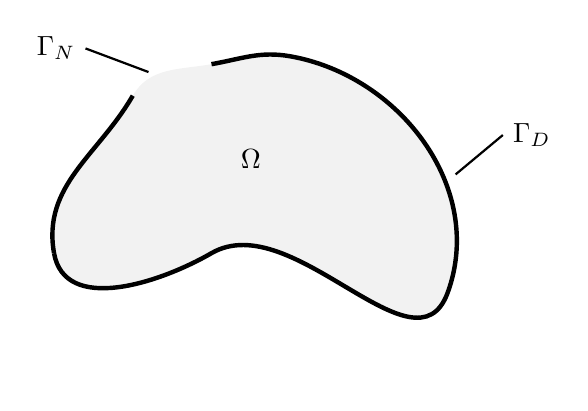
\begin{tikzpicture}
    \fill[black!5!white] (2, 1) to [out=100, in=240] (3, 3)
                              to [out=60, in=190] (4, 3.4)
                              to [out=10, in=170] (5, 3.5)
                              to [out=350, in=70] (7, 0.5)
                              to [out=250, in=30] (4, 1)
                              to [out=210, in=280] (2, 1);
    \draw[ultra thick] (2, 1) to [out=100, in=240] (3, 3);

    \draw[ultra thick] (4, 3.4) to [out=10, in=170] (5, 3.5)
                              to [out=350, in=70] (7, 0.5)
                              to [out=250, in=30] (4, 1)
                              to [out=210, in=280] (2, 1);
    \draw[thick] (2.4, 3.6) node[left] {$\Gamma_N$} to (3.2, 3.3);
    \draw[thick] (7.7, 2.5) node[right] {$\Gamma_D$} to (7.1, 2);
    \node at (4.5, 2.2) {$\Omega$};
\end{tikzpicture}}
            \end{figure}
        \end{column}
        
    \end{columns}

\end{frame}

\begin{frame}{Finite element method | Finite element space}
    \onslide<1->{
        FEniCS \cite{fenics} is used to obtain FEM solutions of the form
        \begin{equation}
            \mathbf{u}_h(\omega) = \sum_{i=1}^{N_h} u_i(\omega) \boldsymbol{\phi}_h^{(i)}
        \end{equation}
        for a basis $\{ \boldsymbol{\phi}_h^{(i)} \}_{i=1}^{N_h}$ of the finite dimensional
        subspace $H_{\text{curl}, h}(\Omega) \subset H_{\text{curl}}(\Omega)$ (Nédélec
        finite elements of the first kind).
    }\onslide<2->{
        From now on
        \begin{equation*}
            \mathbf{u} = (u_1, u_2, \dots, u_{N_h})^T
        \end{equation*}
        with the $L_2(\Omega)$ inner product in $H_{\text{curl}, h}(\Omega)$ represented by
        \begin{equation*}
            \langle \mathbf{u}, \mathbf{v} \rangle_M = \mathbf{u}^H \mathbf{\underline{M}} \mathbf{v}
        \end{equation*}
        and the norm 
        \begin{equation*}
           || \mathbf{u} ||_M = \sqrt{\langle \mathbf{u}, \mathbf{u} \rangle_M}
        \end{equation*}
    }

\end{frame}

\begin{frame}{Minimal rational interpolation | Surrogate}

    \onslide<1->{
        Rational surrogate
        \begin{equation*}
            \mathbf{\tilde{u}}(\omega) = \frac{\mathbf{P}(\omega)}{Q(\omega)} = \sum_{j=1}^S \frac{\mathbf{p}_j}{\omega - \omega_j} / \sum_{j=1}^S \frac{q_j}{\omega - \omega_j}
        \end{equation*}
        in barycentric coordinates with support points $\omega_1$, $\omega_2$, \dots, $\omega_S$.
    }
    \vspace{20pt}
    \onslide<2->{
        Interpolation property
        \begin{equation*}
            \mathbf{\tilde{u}}(\omega_j) = \mathbf{u}(\omega_j),~\forall j \in \{ 1, 2, \dots, S \}
        \end{equation*}
        if and only if $\mathbf{p}_j = q_j\mathbf{u}(\omega_j), \forall j$.
    }

\end{frame}

\begin{frame}{Minimal rational interpolation | MRI algorithm}

    \begin{block}{Minimal rational interpolation (MRI) \cite{greedyMRI}}
        Given snapshots $\mathbf{u}(\omega_1)$, $\mathbf{u}(\omega_2)$, \dots, $\mathbf{u}(\omega_S)$:
        \begin{enumerate}
            \item<2-> Compute the Gramian matrix $\mathbf{\underline{G}}$ with entries $G_{ij} = \langle \mathbf{u}(\omega_i), \mathbf{u}(\omega_j) \rangle_M$, $i,j \in \{1, 2, \dots, S\}$
            \item<3-> Compute the singular value decomposition $\mathbf{\underline{G}} = \mathbf{\underline{V}}~\boldsymbol{\underline{\Sigma}}~\mathbf{\underline{V}}^H$
            \item<4-> Define $\mathbf{q} = (q_1, q_2, \dots, q_S)^T = \mathbf{\underline{V}}[:, S]$
            \item<5-> Define the minimal rational surrogate $\mathbf{\tilde{u}}(\omega) = \mathbf{P}(\omega) / Q(\omega)$ with 
            \begin{equation*}
                \mathbf{P}(\omega) = \sum_{j=1}^S \frac{q_j \mathbf{u}(\omega_j)}{\omega - \omega_j}~~\text{and}~~Q(\omega) = \sum_{j=1}^S \frac{q_j}{\omega - \omega_j}
            \end{equation*}
        \end{enumerate}
    \end{block}

\end{frame}

\begin{frame}{Minimal rational interpolation | gMRI algorithm}
    
    \begin{block}{Greedy minimal rational interpolation (gMRI) \cite{shortMRI}}
        Given $\Omega_{\text{test}} = \{\omega_1, \omega_2, \dots, \omega_T\}$ as candidate support points:
        \begin{enumerate}
            \item<2-> Build the minimal rational surrogate $\mathbf{\tilde{u}}_{2}$
                      with $\mathbf{u}(\omega^{(0)})$ and $\mathbf{u}(\omega^{(1)})$
                      and remove $\omega^{(0)}, \omega^{(1)}$ from $\Omega_{\text{test}}$
            \item<3-> Starting with $t=2$, iteratively take a new support point
            \begin{equation*}
                \omega^{(t+1)} = \text{argmin}_{\omega \in \Omega_{\text{test}}} |Q^{(t)}(\omega)|
            \end{equation*}
            from $\Omega_{\text{test}}$ to build the minimal rational surrogate $\mathbf{\tilde{u}}_{t+1}$
            based on $\mathbf{u}(\omega^{(0)}), \mathbf{u}(\omega^{(1)}), \dots, \mathbf{u}(\omega^{(t+1)})$
            and increment $t$
            \item<4-> Stop when relative error 
            \begin{equation*}
                ||\mathbf{u}(\omega_{t+1}) - \mathbf{\tilde{u}}_{t}(\omega_{t+1})||_M / ||\mathbf{u}(\omega_{t+1})||_M
            \end{equation*}
            is small enough
        \end{enumerate}
    \end{block}

\end{frame}

\begin{frame}{Minimal rational interpolation | Tweak 1}
    
    \onslide<1->{
        With the QR-decomposition of the snapshot matrix $\mathbf{\underline{U}} = [\mathbf{u}(\omega_1), \dots, \mathbf{u}(\omega_S)]^T$.
        \begin{equation*}
            \mathbf{\underline{U}} = \mathbf{\underline{Q}}~\mathbf{\underline{R}}
        \end{equation*}
        the Gramian matrix can be expressed as
        \begin{equation*}
            \mathbf{\underline{G}} = \mathbf{\underline{R}}^H \mathbf{\underline{R}}
        \end{equation*}
    }
    \begin{itemize}
        \item<2-> $\mathbf{\underline{G}}$ and $\mathbf{\underline{R}}$ have
        the same right-singular vector (exactly what is needed for MRI)
        \item<3-> Improved conditioning of SVD with $\mathbf{\underline{R}}$
        \item<4-> $\mathbf{\underline{R}}$ can be built sequentially (modified
        Householder triangularization for gMRI \cite{householder})
    \end{itemize}
    
\end{frame}

\begin{frame}{Minimal rational interpolation | Tweak 2}
    
    \onslide<1->{
        Efficient way of storing the surrogate ($\mathbf{e}_j$ canonical basis vector)
        \begin{equation*}
            \accentset{\circ}{\mathbf{u}}(\omega) = \sum_{j=1}^S \frac{q_j \mathbf{e}_j}{\omega - \omega_j}
            / \sum_{j=1}^S \frac{q_j}{\omega - \omega_j}
        \end{equation*}
    }
    \onslide<2->{
        The original surrogate can be recovered with
        \begin{equation*}
            \mathbf{\tilde{u}}(\omega) = \mathbf{\underline{U}} \accentset{\circ}{\mathbf{u}}(\omega)
        \end{equation*}
    }
    \begin{tikzpicture}[scale=0.7, every node/.style={scale=0.7}]
        \fill[white] (-7.5, -1) rectangle (7.5, 2);
        \node at (4.5, 0) {$\mathbf{\tilde{u}}(\omega) = \frac{\mathbf{P}(\omega)}{Q(\omega)} = \sum_{j=1}^S \frac{q_j\mathbf{u}(\omega_j)}{\omega - \omega_j} / \sum_{j=1}^S \frac{q_j}{\omega - \omega_j}$};
    \end{tikzpicture}
\end{frame}

\begin{frame}{Minimal rational interpolation | Tweak 3}
    
    \onslide<1->{
        Neat helper quantity ($\mathbf{r}_j = \mathbf{\underline{R}}[:, j]$ from QR-decomposition)
        \begin{equation*}
            \mathbf{\hat{u}}(\omega) = \sum_{j=1}^S \frac{q_j \mathbf{r}_j}{\omega - \omega_j}
            / \sum_{j=1}^S \frac{q_j}{\omega - \omega_j}
        \end{equation*}
    }
    \onslide<2->{
        The original surrogate can be recovered with
        \begin{equation*}
            \mathbf{\tilde{u}}(\omega) = \mathbf{\underline{Q}} \mathbf{\hat{u}}(\omega)
        \end{equation*}
    }
    \onslide<3->{
        Proposed way of approximating relative error in gMRI
        \begin{equation*}
            \frac{||\mathbf{u}(\omega_{t+1}) - \mathbf{\tilde{u}}_t(\omega_{t+1})||_M}{||\mathbf{u}(\omega_{t+1})||_M}
            \approx \frac{||\mathbf{r}_{t+1} - \mathbf{\hat{u}}_t(\omega_{t+1})||}{||\mathbf{\hat{u}_t}(\omega_{t+1})||}
        \end{equation*}
    }


\end{frame}

\begin{frame}{Example application 1 | Rectangular cavity}

    \begin{figure}
        \centering
        \scalebox{0.9}{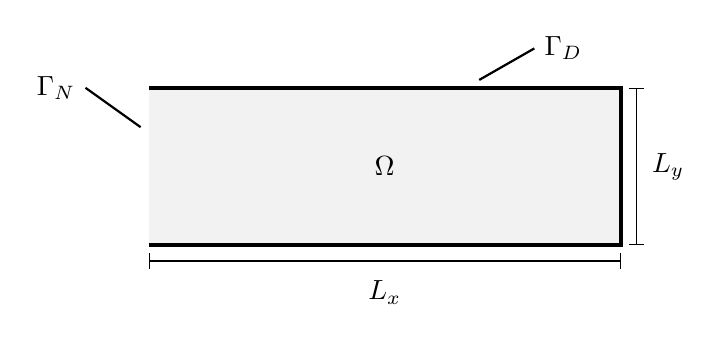
\begin{tikzpicture}
    \fill[black!5!white] (0, 0) rectangle (6, 2);
    \draw[ultra thick] (0, 0) to (6, 0) to (6, 2) to (0, 2);
    \draw[thick] (-0.8, 2) node[left] {$\Gamma_N$} to (-0.1, 1.5);
    \draw[thick] (4.9, 2.5) node[right] {$\Gamma_D$} to (4.2, 2.1);
    \draw[|-|] (0, -0.2) to (6, -0.2);
    \draw[|-|] (6.2, 0) to (6.2, 2);
    \node at (3, -0.6) {$L_x$};
    \node at (6.6, 1) {$L_y$};
    \node at (3, 1) {$\Omega$};
\end{tikzpicture}
}
    \end{figure}
    \vspace{-45pt}
    \begin{figure}
        \centering
        \includegraphics[scale=0.9]{../report/plots/rectangular_cavity_mode1.pdf}
    \end{figure}

\end{frame}

\begin{frame}{Example application 1 | Error progression}

    \begin{figure}
        \centering
        \scalebox{0.8}{\input{../report/plots/rectangular_cavity_errorprogression_presentation.pgf}}
    \end{figure}

\end{frame}

\begin{frame}{Example application 1 | Resonances}

    \begin{figure}
        \centering
        \scalebox{0.8}{%% Creator: Matplotlib, PGF backend
%%
%% To include the figure in your LaTeX document, write
%%   \input{<filename>.pgf}
%%
%% Make sure the required packages are loaded in your preamble
%%   \usepackage{pgf}
%%
%% Also ensure that all the required font packages are loaded; for instance,
%% the lmodern package is sometimes necessary when using math font.
%%   \usepackage{lmodern}
%%
%% Figures using additional raster images can only be included by \input if
%% they are in the same directory as the main LaTeX file. For loading figures
%% from other directories you can use the `import` package
%%   \usepackage{import}
%%
%% and then include the figures with
%%   \import{<path to file>}{<filename>.pgf}
%%
%% Matplotlib used the following preamble
%%   \usepackage{fontspec}
%%   \setmainfont{DejaVuSans.ttf}[Path=\detokenize{C:/Users/Fabio/Anaconda3/Lib/site-packages/matplotlib/mpl-data/fonts/ttf/}]
%%   \setsansfont{DejaVuSans.ttf}[Path=\detokenize{C:/Users/Fabio/Anaconda3/Lib/site-packages/matplotlib/mpl-data/fonts/ttf/}]
%%   \setmonofont{DejaVuSansMono.ttf}[Path=\detokenize{C:/Users/Fabio/Anaconda3/Lib/site-packages/matplotlib/mpl-data/fonts/ttf/}]
%%
\begingroup%
\makeatletter%
\begin{pgfpicture}%
\pgfpathrectangle{\pgfpointorigin}{\pgfqpoint{5.404207in}{3.668486in}}%
\pgfusepath{use as bounding box, clip}%
\begin{pgfscope}%
\pgfsetbuttcap%
\pgfsetmiterjoin%
\pgfsetlinewidth{0.000000pt}%
\definecolor{currentstroke}{rgb}{1.000000,1.000000,1.000000}%
\pgfsetstrokecolor{currentstroke}%
\pgfsetstrokeopacity{0.000000}%
\pgfsetdash{}{0pt}%
\pgfpathmoveto{\pgfqpoint{0.000000in}{0.000000in}}%
\pgfpathlineto{\pgfqpoint{5.404207in}{0.000000in}}%
\pgfpathlineto{\pgfqpoint{5.404207in}{3.668486in}}%
\pgfpathlineto{\pgfqpoint{0.000000in}{3.668486in}}%
\pgfpathlineto{\pgfqpoint{0.000000in}{0.000000in}}%
\pgfpathclose%
\pgfusepath{}%
\end{pgfscope}%
\begin{pgfscope}%
\pgfsetbuttcap%
\pgfsetmiterjoin%
\definecolor{currentfill}{rgb}{1.000000,1.000000,1.000000}%
\pgfsetfillcolor{currentfill}%
\pgfsetlinewidth{0.000000pt}%
\definecolor{currentstroke}{rgb}{0.000000,0.000000,0.000000}%
\pgfsetstrokecolor{currentstroke}%
\pgfsetstrokeopacity{0.000000}%
\pgfsetdash{}{0pt}%
\pgfpathmoveto{\pgfqpoint{0.905793in}{2.406947in}}%
\pgfpathlineto{\pgfqpoint{5.207043in}{2.406947in}}%
\pgfpathlineto{\pgfqpoint{5.207043in}{3.568486in}}%
\pgfpathlineto{\pgfqpoint{0.905793in}{3.568486in}}%
\pgfpathlineto{\pgfqpoint{0.905793in}{2.406947in}}%
\pgfpathclose%
\pgfusepath{fill}%
\end{pgfscope}%
\begin{pgfscope}%
\pgfsetbuttcap%
\pgfsetroundjoin%
\definecolor{currentfill}{rgb}{0.000000,0.000000,0.000000}%
\pgfsetfillcolor{currentfill}%
\pgfsetlinewidth{0.803000pt}%
\definecolor{currentstroke}{rgb}{0.000000,0.000000,0.000000}%
\pgfsetstrokecolor{currentstroke}%
\pgfsetdash{}{0pt}%
\pgfsys@defobject{currentmarker}{\pgfqpoint{0.000000in}{-0.048611in}}{\pgfqpoint{0.000000in}{0.000000in}}{%
\pgfpathmoveto{\pgfqpoint{0.000000in}{0.000000in}}%
\pgfpathlineto{\pgfqpoint{0.000000in}{-0.048611in}}%
\pgfusepath{stroke,fill}%
}%
\begin{pgfscope}%
\pgfsys@transformshift{0.905793in}{2.406947in}%
\pgfsys@useobject{currentmarker}{}%
\end{pgfscope}%
\end{pgfscope}%
\begin{pgfscope}%
\pgfsetbuttcap%
\pgfsetroundjoin%
\definecolor{currentfill}{rgb}{0.000000,0.000000,0.000000}%
\pgfsetfillcolor{currentfill}%
\pgfsetlinewidth{0.803000pt}%
\definecolor{currentstroke}{rgb}{0.000000,0.000000,0.000000}%
\pgfsetstrokecolor{currentstroke}%
\pgfsetdash{}{0pt}%
\pgfsys@defobject{currentmarker}{\pgfqpoint{0.000000in}{-0.048611in}}{\pgfqpoint{0.000000in}{0.000000in}}{%
\pgfpathmoveto{\pgfqpoint{0.000000in}{0.000000in}}%
\pgfpathlineto{\pgfqpoint{0.000000in}{-0.048611in}}%
\pgfusepath{stroke,fill}%
}%
\begin{pgfscope}%
\pgfsys@transformshift{1.766043in}{2.406947in}%
\pgfsys@useobject{currentmarker}{}%
\end{pgfscope}%
\end{pgfscope}%
\begin{pgfscope}%
\pgfsetbuttcap%
\pgfsetroundjoin%
\definecolor{currentfill}{rgb}{0.000000,0.000000,0.000000}%
\pgfsetfillcolor{currentfill}%
\pgfsetlinewidth{0.803000pt}%
\definecolor{currentstroke}{rgb}{0.000000,0.000000,0.000000}%
\pgfsetstrokecolor{currentstroke}%
\pgfsetdash{}{0pt}%
\pgfsys@defobject{currentmarker}{\pgfqpoint{0.000000in}{-0.048611in}}{\pgfqpoint{0.000000in}{0.000000in}}{%
\pgfpathmoveto{\pgfqpoint{0.000000in}{0.000000in}}%
\pgfpathlineto{\pgfqpoint{0.000000in}{-0.048611in}}%
\pgfusepath{stroke,fill}%
}%
\begin{pgfscope}%
\pgfsys@transformshift{2.626293in}{2.406947in}%
\pgfsys@useobject{currentmarker}{}%
\end{pgfscope}%
\end{pgfscope}%
\begin{pgfscope}%
\pgfsetbuttcap%
\pgfsetroundjoin%
\definecolor{currentfill}{rgb}{0.000000,0.000000,0.000000}%
\pgfsetfillcolor{currentfill}%
\pgfsetlinewidth{0.803000pt}%
\definecolor{currentstroke}{rgb}{0.000000,0.000000,0.000000}%
\pgfsetstrokecolor{currentstroke}%
\pgfsetdash{}{0pt}%
\pgfsys@defobject{currentmarker}{\pgfqpoint{0.000000in}{-0.048611in}}{\pgfqpoint{0.000000in}{0.000000in}}{%
\pgfpathmoveto{\pgfqpoint{0.000000in}{0.000000in}}%
\pgfpathlineto{\pgfqpoint{0.000000in}{-0.048611in}}%
\pgfusepath{stroke,fill}%
}%
\begin{pgfscope}%
\pgfsys@transformshift{3.486543in}{2.406947in}%
\pgfsys@useobject{currentmarker}{}%
\end{pgfscope}%
\end{pgfscope}%
\begin{pgfscope}%
\pgfsetbuttcap%
\pgfsetroundjoin%
\definecolor{currentfill}{rgb}{0.000000,0.000000,0.000000}%
\pgfsetfillcolor{currentfill}%
\pgfsetlinewidth{0.803000pt}%
\definecolor{currentstroke}{rgb}{0.000000,0.000000,0.000000}%
\pgfsetstrokecolor{currentstroke}%
\pgfsetdash{}{0pt}%
\pgfsys@defobject{currentmarker}{\pgfqpoint{0.000000in}{-0.048611in}}{\pgfqpoint{0.000000in}{0.000000in}}{%
\pgfpathmoveto{\pgfqpoint{0.000000in}{0.000000in}}%
\pgfpathlineto{\pgfqpoint{0.000000in}{-0.048611in}}%
\pgfusepath{stroke,fill}%
}%
\begin{pgfscope}%
\pgfsys@transformshift{4.346793in}{2.406947in}%
\pgfsys@useobject{currentmarker}{}%
\end{pgfscope}%
\end{pgfscope}%
\begin{pgfscope}%
\pgfsetbuttcap%
\pgfsetroundjoin%
\definecolor{currentfill}{rgb}{0.000000,0.000000,0.000000}%
\pgfsetfillcolor{currentfill}%
\pgfsetlinewidth{0.803000pt}%
\definecolor{currentstroke}{rgb}{0.000000,0.000000,0.000000}%
\pgfsetstrokecolor{currentstroke}%
\pgfsetdash{}{0pt}%
\pgfsys@defobject{currentmarker}{\pgfqpoint{0.000000in}{-0.048611in}}{\pgfqpoint{0.000000in}{0.000000in}}{%
\pgfpathmoveto{\pgfqpoint{0.000000in}{0.000000in}}%
\pgfpathlineto{\pgfqpoint{0.000000in}{-0.048611in}}%
\pgfusepath{stroke,fill}%
}%
\begin{pgfscope}%
\pgfsys@transformshift{5.207043in}{2.406947in}%
\pgfsys@useobject{currentmarker}{}%
\end{pgfscope}%
\end{pgfscope}%
\begin{pgfscope}%
\pgfsetbuttcap%
\pgfsetroundjoin%
\definecolor{currentfill}{rgb}{0.000000,0.000000,0.000000}%
\pgfsetfillcolor{currentfill}%
\pgfsetlinewidth{0.803000pt}%
\definecolor{currentstroke}{rgb}{0.000000,0.000000,0.000000}%
\pgfsetstrokecolor{currentstroke}%
\pgfsetdash{}{0pt}%
\pgfsys@defobject{currentmarker}{\pgfqpoint{-0.048611in}{0.000000in}}{\pgfqpoint{-0.000000in}{0.000000in}}{%
\pgfpathmoveto{\pgfqpoint{-0.000000in}{0.000000in}}%
\pgfpathlineto{\pgfqpoint{-0.048611in}{0.000000in}}%
\pgfusepath{stroke,fill}%
}%
\begin{pgfscope}%
\pgfsys@transformshift{0.905793in}{2.723927in}%
\pgfsys@useobject{currentmarker}{}%
\end{pgfscope}%
\end{pgfscope}%
\begin{pgfscope}%
\definecolor{textcolor}{rgb}{0.000000,0.000000,0.000000}%
\pgfsetstrokecolor{textcolor}%
\pgfsetfillcolor{textcolor}%
\pgftext[x=0.590514in, y=2.665890in, left, base]{\color{textcolor}\rmfamily\fontsize{11.000000}{13.200000}\selectfont \(\displaystyle {10^{0}}\)}%
\end{pgfscope}%
\begin{pgfscope}%
\pgfsetbuttcap%
\pgfsetroundjoin%
\definecolor{currentfill}{rgb}{0.000000,0.000000,0.000000}%
\pgfsetfillcolor{currentfill}%
\pgfsetlinewidth{0.803000pt}%
\definecolor{currentstroke}{rgb}{0.000000,0.000000,0.000000}%
\pgfsetstrokecolor{currentstroke}%
\pgfsetdash{}{0pt}%
\pgfsys@defobject{currentmarker}{\pgfqpoint{-0.048611in}{0.000000in}}{\pgfqpoint{-0.000000in}{0.000000in}}{%
\pgfpathmoveto{\pgfqpoint{-0.000000in}{0.000000in}}%
\pgfpathlineto{\pgfqpoint{-0.048611in}{0.000000in}}%
\pgfusepath{stroke,fill}%
}%
\begin{pgfscope}%
\pgfsys@transformshift{0.905793in}{3.082904in}%
\pgfsys@useobject{currentmarker}{}%
\end{pgfscope}%
\end{pgfscope}%
\begin{pgfscope}%
\definecolor{textcolor}{rgb}{0.000000,0.000000,0.000000}%
\pgfsetstrokecolor{textcolor}%
\pgfsetfillcolor{textcolor}%
\pgftext[x=0.590514in, y=3.024866in, left, base]{\color{textcolor}\rmfamily\fontsize{11.000000}{13.200000}\selectfont \(\displaystyle {10^{1}}\)}%
\end{pgfscope}%
\begin{pgfscope}%
\pgfsetbuttcap%
\pgfsetroundjoin%
\definecolor{currentfill}{rgb}{0.000000,0.000000,0.000000}%
\pgfsetfillcolor{currentfill}%
\pgfsetlinewidth{0.803000pt}%
\definecolor{currentstroke}{rgb}{0.000000,0.000000,0.000000}%
\pgfsetstrokecolor{currentstroke}%
\pgfsetdash{}{0pt}%
\pgfsys@defobject{currentmarker}{\pgfqpoint{-0.048611in}{0.000000in}}{\pgfqpoint{-0.000000in}{0.000000in}}{%
\pgfpathmoveto{\pgfqpoint{-0.000000in}{0.000000in}}%
\pgfpathlineto{\pgfqpoint{-0.048611in}{0.000000in}}%
\pgfusepath{stroke,fill}%
}%
\begin{pgfscope}%
\pgfsys@transformshift{0.905793in}{3.441880in}%
\pgfsys@useobject{currentmarker}{}%
\end{pgfscope}%
\end{pgfscope}%
\begin{pgfscope}%
\definecolor{textcolor}{rgb}{0.000000,0.000000,0.000000}%
\pgfsetstrokecolor{textcolor}%
\pgfsetfillcolor{textcolor}%
\pgftext[x=0.590514in, y=3.383843in, left, base]{\color{textcolor}\rmfamily\fontsize{11.000000}{13.200000}\selectfont \(\displaystyle {10^{2}}\)}%
\end{pgfscope}%
\begin{pgfscope}%
\pgfsetbuttcap%
\pgfsetroundjoin%
\definecolor{currentfill}{rgb}{0.000000,0.000000,0.000000}%
\pgfsetfillcolor{currentfill}%
\pgfsetlinewidth{0.602250pt}%
\definecolor{currentstroke}{rgb}{0.000000,0.000000,0.000000}%
\pgfsetstrokecolor{currentstroke}%
\pgfsetdash{}{0pt}%
\pgfsys@defobject{currentmarker}{\pgfqpoint{-0.027778in}{0.000000in}}{\pgfqpoint{-0.000000in}{0.000000in}}{%
\pgfpathmoveto{\pgfqpoint{-0.000000in}{0.000000in}}%
\pgfpathlineto{\pgfqpoint{-0.027778in}{0.000000in}}%
\pgfusepath{stroke,fill}%
}%
\begin{pgfscope}%
\pgfsys@transformshift{0.905793in}{2.473014in}%
\pgfsys@useobject{currentmarker}{}%
\end{pgfscope}%
\end{pgfscope}%
\begin{pgfscope}%
\pgfsetbuttcap%
\pgfsetroundjoin%
\definecolor{currentfill}{rgb}{0.000000,0.000000,0.000000}%
\pgfsetfillcolor{currentfill}%
\pgfsetlinewidth{0.602250pt}%
\definecolor{currentstroke}{rgb}{0.000000,0.000000,0.000000}%
\pgfsetstrokecolor{currentstroke}%
\pgfsetdash{}{0pt}%
\pgfsys@defobject{currentmarker}{\pgfqpoint{-0.027778in}{0.000000in}}{\pgfqpoint{-0.000000in}{0.000000in}}{%
\pgfpathmoveto{\pgfqpoint{-0.000000in}{0.000000in}}%
\pgfpathlineto{\pgfqpoint{-0.027778in}{0.000000in}}%
\pgfusepath{stroke,fill}%
}%
\begin{pgfscope}%
\pgfsys@transformshift{0.905793in}{2.536226in}%
\pgfsys@useobject{currentmarker}{}%
\end{pgfscope}%
\end{pgfscope}%
\begin{pgfscope}%
\pgfsetbuttcap%
\pgfsetroundjoin%
\definecolor{currentfill}{rgb}{0.000000,0.000000,0.000000}%
\pgfsetfillcolor{currentfill}%
\pgfsetlinewidth{0.602250pt}%
\definecolor{currentstroke}{rgb}{0.000000,0.000000,0.000000}%
\pgfsetstrokecolor{currentstroke}%
\pgfsetdash{}{0pt}%
\pgfsys@defobject{currentmarker}{\pgfqpoint{-0.027778in}{0.000000in}}{\pgfqpoint{-0.000000in}{0.000000in}}{%
\pgfpathmoveto{\pgfqpoint{-0.000000in}{0.000000in}}%
\pgfpathlineto{\pgfqpoint{-0.027778in}{0.000000in}}%
\pgfusepath{stroke,fill}%
}%
\begin{pgfscope}%
\pgfsys@transformshift{0.905793in}{2.581076in}%
\pgfsys@useobject{currentmarker}{}%
\end{pgfscope}%
\end{pgfscope}%
\begin{pgfscope}%
\pgfsetbuttcap%
\pgfsetroundjoin%
\definecolor{currentfill}{rgb}{0.000000,0.000000,0.000000}%
\pgfsetfillcolor{currentfill}%
\pgfsetlinewidth{0.602250pt}%
\definecolor{currentstroke}{rgb}{0.000000,0.000000,0.000000}%
\pgfsetstrokecolor{currentstroke}%
\pgfsetdash{}{0pt}%
\pgfsys@defobject{currentmarker}{\pgfqpoint{-0.027778in}{0.000000in}}{\pgfqpoint{-0.000000in}{0.000000in}}{%
\pgfpathmoveto{\pgfqpoint{-0.000000in}{0.000000in}}%
\pgfpathlineto{\pgfqpoint{-0.027778in}{0.000000in}}%
\pgfusepath{stroke,fill}%
}%
\begin{pgfscope}%
\pgfsys@transformshift{0.905793in}{2.615865in}%
\pgfsys@useobject{currentmarker}{}%
\end{pgfscope}%
\end{pgfscope}%
\begin{pgfscope}%
\pgfsetbuttcap%
\pgfsetroundjoin%
\definecolor{currentfill}{rgb}{0.000000,0.000000,0.000000}%
\pgfsetfillcolor{currentfill}%
\pgfsetlinewidth{0.602250pt}%
\definecolor{currentstroke}{rgb}{0.000000,0.000000,0.000000}%
\pgfsetstrokecolor{currentstroke}%
\pgfsetdash{}{0pt}%
\pgfsys@defobject{currentmarker}{\pgfqpoint{-0.027778in}{0.000000in}}{\pgfqpoint{-0.000000in}{0.000000in}}{%
\pgfpathmoveto{\pgfqpoint{-0.000000in}{0.000000in}}%
\pgfpathlineto{\pgfqpoint{-0.027778in}{0.000000in}}%
\pgfusepath{stroke,fill}%
}%
\begin{pgfscope}%
\pgfsys@transformshift{0.905793in}{2.644289in}%
\pgfsys@useobject{currentmarker}{}%
\end{pgfscope}%
\end{pgfscope}%
\begin{pgfscope}%
\pgfsetbuttcap%
\pgfsetroundjoin%
\definecolor{currentfill}{rgb}{0.000000,0.000000,0.000000}%
\pgfsetfillcolor{currentfill}%
\pgfsetlinewidth{0.602250pt}%
\definecolor{currentstroke}{rgb}{0.000000,0.000000,0.000000}%
\pgfsetstrokecolor{currentstroke}%
\pgfsetdash{}{0pt}%
\pgfsys@defobject{currentmarker}{\pgfqpoint{-0.027778in}{0.000000in}}{\pgfqpoint{-0.000000in}{0.000000in}}{%
\pgfpathmoveto{\pgfqpoint{-0.000000in}{0.000000in}}%
\pgfpathlineto{\pgfqpoint{-0.027778in}{0.000000in}}%
\pgfusepath{stroke,fill}%
}%
\begin{pgfscope}%
\pgfsys@transformshift{0.905793in}{2.668321in}%
\pgfsys@useobject{currentmarker}{}%
\end{pgfscope}%
\end{pgfscope}%
\begin{pgfscope}%
\pgfsetbuttcap%
\pgfsetroundjoin%
\definecolor{currentfill}{rgb}{0.000000,0.000000,0.000000}%
\pgfsetfillcolor{currentfill}%
\pgfsetlinewidth{0.602250pt}%
\definecolor{currentstroke}{rgb}{0.000000,0.000000,0.000000}%
\pgfsetstrokecolor{currentstroke}%
\pgfsetdash{}{0pt}%
\pgfsys@defobject{currentmarker}{\pgfqpoint{-0.027778in}{0.000000in}}{\pgfqpoint{-0.000000in}{0.000000in}}{%
\pgfpathmoveto{\pgfqpoint{-0.000000in}{0.000000in}}%
\pgfpathlineto{\pgfqpoint{-0.027778in}{0.000000in}}%
\pgfusepath{stroke,fill}%
}%
\begin{pgfscope}%
\pgfsys@transformshift{0.905793in}{2.689139in}%
\pgfsys@useobject{currentmarker}{}%
\end{pgfscope}%
\end{pgfscope}%
\begin{pgfscope}%
\pgfsetbuttcap%
\pgfsetroundjoin%
\definecolor{currentfill}{rgb}{0.000000,0.000000,0.000000}%
\pgfsetfillcolor{currentfill}%
\pgfsetlinewidth{0.602250pt}%
\definecolor{currentstroke}{rgb}{0.000000,0.000000,0.000000}%
\pgfsetstrokecolor{currentstroke}%
\pgfsetdash{}{0pt}%
\pgfsys@defobject{currentmarker}{\pgfqpoint{-0.027778in}{0.000000in}}{\pgfqpoint{-0.000000in}{0.000000in}}{%
\pgfpathmoveto{\pgfqpoint{-0.000000in}{0.000000in}}%
\pgfpathlineto{\pgfqpoint{-0.027778in}{0.000000in}}%
\pgfusepath{stroke,fill}%
}%
\begin{pgfscope}%
\pgfsys@transformshift{0.905793in}{2.707502in}%
\pgfsys@useobject{currentmarker}{}%
\end{pgfscope}%
\end{pgfscope}%
\begin{pgfscope}%
\pgfsetbuttcap%
\pgfsetroundjoin%
\definecolor{currentfill}{rgb}{0.000000,0.000000,0.000000}%
\pgfsetfillcolor{currentfill}%
\pgfsetlinewidth{0.602250pt}%
\definecolor{currentstroke}{rgb}{0.000000,0.000000,0.000000}%
\pgfsetstrokecolor{currentstroke}%
\pgfsetdash{}{0pt}%
\pgfsys@defobject{currentmarker}{\pgfqpoint{-0.027778in}{0.000000in}}{\pgfqpoint{-0.000000in}{0.000000in}}{%
\pgfpathmoveto{\pgfqpoint{-0.000000in}{0.000000in}}%
\pgfpathlineto{\pgfqpoint{-0.027778in}{0.000000in}}%
\pgfusepath{stroke,fill}%
}%
\begin{pgfscope}%
\pgfsys@transformshift{0.905793in}{2.831990in}%
\pgfsys@useobject{currentmarker}{}%
\end{pgfscope}%
\end{pgfscope}%
\begin{pgfscope}%
\pgfsetbuttcap%
\pgfsetroundjoin%
\definecolor{currentfill}{rgb}{0.000000,0.000000,0.000000}%
\pgfsetfillcolor{currentfill}%
\pgfsetlinewidth{0.602250pt}%
\definecolor{currentstroke}{rgb}{0.000000,0.000000,0.000000}%
\pgfsetstrokecolor{currentstroke}%
\pgfsetdash{}{0pt}%
\pgfsys@defobject{currentmarker}{\pgfqpoint{-0.027778in}{0.000000in}}{\pgfqpoint{-0.000000in}{0.000000in}}{%
\pgfpathmoveto{\pgfqpoint{-0.000000in}{0.000000in}}%
\pgfpathlineto{\pgfqpoint{-0.027778in}{0.000000in}}%
\pgfusepath{stroke,fill}%
}%
\begin{pgfscope}%
\pgfsys@transformshift{0.905793in}{2.895203in}%
\pgfsys@useobject{currentmarker}{}%
\end{pgfscope}%
\end{pgfscope}%
\begin{pgfscope}%
\pgfsetbuttcap%
\pgfsetroundjoin%
\definecolor{currentfill}{rgb}{0.000000,0.000000,0.000000}%
\pgfsetfillcolor{currentfill}%
\pgfsetlinewidth{0.602250pt}%
\definecolor{currentstroke}{rgb}{0.000000,0.000000,0.000000}%
\pgfsetstrokecolor{currentstroke}%
\pgfsetdash{}{0pt}%
\pgfsys@defobject{currentmarker}{\pgfqpoint{-0.027778in}{0.000000in}}{\pgfqpoint{-0.000000in}{0.000000in}}{%
\pgfpathmoveto{\pgfqpoint{-0.000000in}{0.000000in}}%
\pgfpathlineto{\pgfqpoint{-0.027778in}{0.000000in}}%
\pgfusepath{stroke,fill}%
}%
\begin{pgfscope}%
\pgfsys@transformshift{0.905793in}{2.940053in}%
\pgfsys@useobject{currentmarker}{}%
\end{pgfscope}%
\end{pgfscope}%
\begin{pgfscope}%
\pgfsetbuttcap%
\pgfsetroundjoin%
\definecolor{currentfill}{rgb}{0.000000,0.000000,0.000000}%
\pgfsetfillcolor{currentfill}%
\pgfsetlinewidth{0.602250pt}%
\definecolor{currentstroke}{rgb}{0.000000,0.000000,0.000000}%
\pgfsetstrokecolor{currentstroke}%
\pgfsetdash{}{0pt}%
\pgfsys@defobject{currentmarker}{\pgfqpoint{-0.027778in}{0.000000in}}{\pgfqpoint{-0.000000in}{0.000000in}}{%
\pgfpathmoveto{\pgfqpoint{-0.000000in}{0.000000in}}%
\pgfpathlineto{\pgfqpoint{-0.027778in}{0.000000in}}%
\pgfusepath{stroke,fill}%
}%
\begin{pgfscope}%
\pgfsys@transformshift{0.905793in}{2.974841in}%
\pgfsys@useobject{currentmarker}{}%
\end{pgfscope}%
\end{pgfscope}%
\begin{pgfscope}%
\pgfsetbuttcap%
\pgfsetroundjoin%
\definecolor{currentfill}{rgb}{0.000000,0.000000,0.000000}%
\pgfsetfillcolor{currentfill}%
\pgfsetlinewidth{0.602250pt}%
\definecolor{currentstroke}{rgb}{0.000000,0.000000,0.000000}%
\pgfsetstrokecolor{currentstroke}%
\pgfsetdash{}{0pt}%
\pgfsys@defobject{currentmarker}{\pgfqpoint{-0.027778in}{0.000000in}}{\pgfqpoint{-0.000000in}{0.000000in}}{%
\pgfpathmoveto{\pgfqpoint{-0.000000in}{0.000000in}}%
\pgfpathlineto{\pgfqpoint{-0.027778in}{0.000000in}}%
\pgfusepath{stroke,fill}%
}%
\begin{pgfscope}%
\pgfsys@transformshift{0.905793in}{3.003265in}%
\pgfsys@useobject{currentmarker}{}%
\end{pgfscope}%
\end{pgfscope}%
\begin{pgfscope}%
\pgfsetbuttcap%
\pgfsetroundjoin%
\definecolor{currentfill}{rgb}{0.000000,0.000000,0.000000}%
\pgfsetfillcolor{currentfill}%
\pgfsetlinewidth{0.602250pt}%
\definecolor{currentstroke}{rgb}{0.000000,0.000000,0.000000}%
\pgfsetstrokecolor{currentstroke}%
\pgfsetdash{}{0pt}%
\pgfsys@defobject{currentmarker}{\pgfqpoint{-0.027778in}{0.000000in}}{\pgfqpoint{-0.000000in}{0.000000in}}{%
\pgfpathmoveto{\pgfqpoint{-0.000000in}{0.000000in}}%
\pgfpathlineto{\pgfqpoint{-0.027778in}{0.000000in}}%
\pgfusepath{stroke,fill}%
}%
\begin{pgfscope}%
\pgfsys@transformshift{0.905793in}{3.027298in}%
\pgfsys@useobject{currentmarker}{}%
\end{pgfscope}%
\end{pgfscope}%
\begin{pgfscope}%
\pgfsetbuttcap%
\pgfsetroundjoin%
\definecolor{currentfill}{rgb}{0.000000,0.000000,0.000000}%
\pgfsetfillcolor{currentfill}%
\pgfsetlinewidth{0.602250pt}%
\definecolor{currentstroke}{rgb}{0.000000,0.000000,0.000000}%
\pgfsetstrokecolor{currentstroke}%
\pgfsetdash{}{0pt}%
\pgfsys@defobject{currentmarker}{\pgfqpoint{-0.027778in}{0.000000in}}{\pgfqpoint{-0.000000in}{0.000000in}}{%
\pgfpathmoveto{\pgfqpoint{-0.000000in}{0.000000in}}%
\pgfpathlineto{\pgfqpoint{-0.027778in}{0.000000in}}%
\pgfusepath{stroke,fill}%
}%
\begin{pgfscope}%
\pgfsys@transformshift{0.905793in}{3.048115in}%
\pgfsys@useobject{currentmarker}{}%
\end{pgfscope}%
\end{pgfscope}%
\begin{pgfscope}%
\pgfsetbuttcap%
\pgfsetroundjoin%
\definecolor{currentfill}{rgb}{0.000000,0.000000,0.000000}%
\pgfsetfillcolor{currentfill}%
\pgfsetlinewidth{0.602250pt}%
\definecolor{currentstroke}{rgb}{0.000000,0.000000,0.000000}%
\pgfsetstrokecolor{currentstroke}%
\pgfsetdash{}{0pt}%
\pgfsys@defobject{currentmarker}{\pgfqpoint{-0.027778in}{0.000000in}}{\pgfqpoint{-0.000000in}{0.000000in}}{%
\pgfpathmoveto{\pgfqpoint{-0.000000in}{0.000000in}}%
\pgfpathlineto{\pgfqpoint{-0.027778in}{0.000000in}}%
\pgfusepath{stroke,fill}%
}%
\begin{pgfscope}%
\pgfsys@transformshift{0.905793in}{3.066478in}%
\pgfsys@useobject{currentmarker}{}%
\end{pgfscope}%
\end{pgfscope}%
\begin{pgfscope}%
\pgfsetbuttcap%
\pgfsetroundjoin%
\definecolor{currentfill}{rgb}{0.000000,0.000000,0.000000}%
\pgfsetfillcolor{currentfill}%
\pgfsetlinewidth{0.602250pt}%
\definecolor{currentstroke}{rgb}{0.000000,0.000000,0.000000}%
\pgfsetstrokecolor{currentstroke}%
\pgfsetdash{}{0pt}%
\pgfsys@defobject{currentmarker}{\pgfqpoint{-0.027778in}{0.000000in}}{\pgfqpoint{-0.000000in}{0.000000in}}{%
\pgfpathmoveto{\pgfqpoint{-0.000000in}{0.000000in}}%
\pgfpathlineto{\pgfqpoint{-0.027778in}{0.000000in}}%
\pgfusepath{stroke,fill}%
}%
\begin{pgfscope}%
\pgfsys@transformshift{0.905793in}{3.190966in}%
\pgfsys@useobject{currentmarker}{}%
\end{pgfscope}%
\end{pgfscope}%
\begin{pgfscope}%
\pgfsetbuttcap%
\pgfsetroundjoin%
\definecolor{currentfill}{rgb}{0.000000,0.000000,0.000000}%
\pgfsetfillcolor{currentfill}%
\pgfsetlinewidth{0.602250pt}%
\definecolor{currentstroke}{rgb}{0.000000,0.000000,0.000000}%
\pgfsetstrokecolor{currentstroke}%
\pgfsetdash{}{0pt}%
\pgfsys@defobject{currentmarker}{\pgfqpoint{-0.027778in}{0.000000in}}{\pgfqpoint{-0.000000in}{0.000000in}}{%
\pgfpathmoveto{\pgfqpoint{-0.000000in}{0.000000in}}%
\pgfpathlineto{\pgfqpoint{-0.027778in}{0.000000in}}%
\pgfusepath{stroke,fill}%
}%
\begin{pgfscope}%
\pgfsys@transformshift{0.905793in}{3.254179in}%
\pgfsys@useobject{currentmarker}{}%
\end{pgfscope}%
\end{pgfscope}%
\begin{pgfscope}%
\pgfsetbuttcap%
\pgfsetroundjoin%
\definecolor{currentfill}{rgb}{0.000000,0.000000,0.000000}%
\pgfsetfillcolor{currentfill}%
\pgfsetlinewidth{0.602250pt}%
\definecolor{currentstroke}{rgb}{0.000000,0.000000,0.000000}%
\pgfsetstrokecolor{currentstroke}%
\pgfsetdash{}{0pt}%
\pgfsys@defobject{currentmarker}{\pgfqpoint{-0.027778in}{0.000000in}}{\pgfqpoint{-0.000000in}{0.000000in}}{%
\pgfpathmoveto{\pgfqpoint{-0.000000in}{0.000000in}}%
\pgfpathlineto{\pgfqpoint{-0.027778in}{0.000000in}}%
\pgfusepath{stroke,fill}%
}%
\begin{pgfscope}%
\pgfsys@transformshift{0.905793in}{3.299029in}%
\pgfsys@useobject{currentmarker}{}%
\end{pgfscope}%
\end{pgfscope}%
\begin{pgfscope}%
\pgfsetbuttcap%
\pgfsetroundjoin%
\definecolor{currentfill}{rgb}{0.000000,0.000000,0.000000}%
\pgfsetfillcolor{currentfill}%
\pgfsetlinewidth{0.602250pt}%
\definecolor{currentstroke}{rgb}{0.000000,0.000000,0.000000}%
\pgfsetstrokecolor{currentstroke}%
\pgfsetdash{}{0pt}%
\pgfsys@defobject{currentmarker}{\pgfqpoint{-0.027778in}{0.000000in}}{\pgfqpoint{-0.000000in}{0.000000in}}{%
\pgfpathmoveto{\pgfqpoint{-0.000000in}{0.000000in}}%
\pgfpathlineto{\pgfqpoint{-0.027778in}{0.000000in}}%
\pgfusepath{stroke,fill}%
}%
\begin{pgfscope}%
\pgfsys@transformshift{0.905793in}{3.333818in}%
\pgfsys@useobject{currentmarker}{}%
\end{pgfscope}%
\end{pgfscope}%
\begin{pgfscope}%
\pgfsetbuttcap%
\pgfsetroundjoin%
\definecolor{currentfill}{rgb}{0.000000,0.000000,0.000000}%
\pgfsetfillcolor{currentfill}%
\pgfsetlinewidth{0.602250pt}%
\definecolor{currentstroke}{rgb}{0.000000,0.000000,0.000000}%
\pgfsetstrokecolor{currentstroke}%
\pgfsetdash{}{0pt}%
\pgfsys@defobject{currentmarker}{\pgfqpoint{-0.027778in}{0.000000in}}{\pgfqpoint{-0.000000in}{0.000000in}}{%
\pgfpathmoveto{\pgfqpoint{-0.000000in}{0.000000in}}%
\pgfpathlineto{\pgfqpoint{-0.027778in}{0.000000in}}%
\pgfusepath{stroke,fill}%
}%
\begin{pgfscope}%
\pgfsys@transformshift{0.905793in}{3.362242in}%
\pgfsys@useobject{currentmarker}{}%
\end{pgfscope}%
\end{pgfscope}%
\begin{pgfscope}%
\pgfsetbuttcap%
\pgfsetroundjoin%
\definecolor{currentfill}{rgb}{0.000000,0.000000,0.000000}%
\pgfsetfillcolor{currentfill}%
\pgfsetlinewidth{0.602250pt}%
\definecolor{currentstroke}{rgb}{0.000000,0.000000,0.000000}%
\pgfsetstrokecolor{currentstroke}%
\pgfsetdash{}{0pt}%
\pgfsys@defobject{currentmarker}{\pgfqpoint{-0.027778in}{0.000000in}}{\pgfqpoint{-0.000000in}{0.000000in}}{%
\pgfpathmoveto{\pgfqpoint{-0.000000in}{0.000000in}}%
\pgfpathlineto{\pgfqpoint{-0.027778in}{0.000000in}}%
\pgfusepath{stroke,fill}%
}%
\begin{pgfscope}%
\pgfsys@transformshift{0.905793in}{3.386274in}%
\pgfsys@useobject{currentmarker}{}%
\end{pgfscope}%
\end{pgfscope}%
\begin{pgfscope}%
\pgfsetbuttcap%
\pgfsetroundjoin%
\definecolor{currentfill}{rgb}{0.000000,0.000000,0.000000}%
\pgfsetfillcolor{currentfill}%
\pgfsetlinewidth{0.602250pt}%
\definecolor{currentstroke}{rgb}{0.000000,0.000000,0.000000}%
\pgfsetstrokecolor{currentstroke}%
\pgfsetdash{}{0pt}%
\pgfsys@defobject{currentmarker}{\pgfqpoint{-0.027778in}{0.000000in}}{\pgfqpoint{-0.000000in}{0.000000in}}{%
\pgfpathmoveto{\pgfqpoint{-0.000000in}{0.000000in}}%
\pgfpathlineto{\pgfqpoint{-0.027778in}{0.000000in}}%
\pgfusepath{stroke,fill}%
}%
\begin{pgfscope}%
\pgfsys@transformshift{0.905793in}{3.407092in}%
\pgfsys@useobject{currentmarker}{}%
\end{pgfscope}%
\end{pgfscope}%
\begin{pgfscope}%
\pgfsetbuttcap%
\pgfsetroundjoin%
\definecolor{currentfill}{rgb}{0.000000,0.000000,0.000000}%
\pgfsetfillcolor{currentfill}%
\pgfsetlinewidth{0.602250pt}%
\definecolor{currentstroke}{rgb}{0.000000,0.000000,0.000000}%
\pgfsetstrokecolor{currentstroke}%
\pgfsetdash{}{0pt}%
\pgfsys@defobject{currentmarker}{\pgfqpoint{-0.027778in}{0.000000in}}{\pgfqpoint{-0.000000in}{0.000000in}}{%
\pgfpathmoveto{\pgfqpoint{-0.000000in}{0.000000in}}%
\pgfpathlineto{\pgfqpoint{-0.027778in}{0.000000in}}%
\pgfusepath{stroke,fill}%
}%
\begin{pgfscope}%
\pgfsys@transformshift{0.905793in}{3.425454in}%
\pgfsys@useobject{currentmarker}{}%
\end{pgfscope}%
\end{pgfscope}%
\begin{pgfscope}%
\pgfsetbuttcap%
\pgfsetroundjoin%
\definecolor{currentfill}{rgb}{0.000000,0.000000,0.000000}%
\pgfsetfillcolor{currentfill}%
\pgfsetlinewidth{0.602250pt}%
\definecolor{currentstroke}{rgb}{0.000000,0.000000,0.000000}%
\pgfsetstrokecolor{currentstroke}%
\pgfsetdash{}{0pt}%
\pgfsys@defobject{currentmarker}{\pgfqpoint{-0.027778in}{0.000000in}}{\pgfqpoint{-0.000000in}{0.000000in}}{%
\pgfpathmoveto{\pgfqpoint{-0.000000in}{0.000000in}}%
\pgfpathlineto{\pgfqpoint{-0.027778in}{0.000000in}}%
\pgfusepath{stroke,fill}%
}%
\begin{pgfscope}%
\pgfsys@transformshift{0.905793in}{3.549943in}%
\pgfsys@useobject{currentmarker}{}%
\end{pgfscope}%
\end{pgfscope}%
\begin{pgfscope}%
\definecolor{textcolor}{rgb}{0.000000,0.000000,0.000000}%
\pgfsetstrokecolor{textcolor}%
\pgfsetfillcolor{textcolor}%
\pgftext[x=0.534959in,y=2.987717in,,bottom,rotate=90.000000]{\color{textcolor}\rmfamily\fontsize{11.000000}{13.200000}\selectfont \(\displaystyle ||\mathbf{u}(\omega)||_M\)}%
\end{pgfscope}%
\begin{pgfscope}%
\pgfpathrectangle{\pgfqpoint{0.905793in}{2.406947in}}{\pgfqpoint{4.301250in}{1.161538in}}%
\pgfusepath{clip}%
\pgfsetrectcap%
\pgfsetroundjoin%
\pgfsetlinewidth{1.505625pt}%
\definecolor{currentstroke}{rgb}{0.000000,0.000000,0.000000}%
\pgfsetstrokecolor{currentstroke}%
\pgfsetdash{}{0pt}%
\pgfpathmoveto{\pgfqpoint{0.905793in}{2.495999in}}%
\pgfpathlineto{\pgfqpoint{1.000515in}{2.504161in}}%
\pgfpathlineto{\pgfqpoint{1.090932in}{2.515124in}}%
\pgfpathlineto{\pgfqpoint{1.172737in}{2.528129in}}%
\pgfpathlineto{\pgfqpoint{1.245932in}{2.542710in}}%
\pgfpathlineto{\pgfqpoint{1.314821in}{2.559511in}}%
\pgfpathlineto{\pgfqpoint{1.375098in}{2.577236in}}%
\pgfpathlineto{\pgfqpoint{1.431071in}{2.596881in}}%
\pgfpathlineto{\pgfqpoint{1.478432in}{2.616565in}}%
\pgfpathlineto{\pgfqpoint{1.521487in}{2.637613in}}%
\pgfpathlineto{\pgfqpoint{1.560237in}{2.659921in}}%
\pgfpathlineto{\pgfqpoint{1.594682in}{2.683312in}}%
\pgfpathlineto{\pgfqpoint{1.624821in}{2.707488in}}%
\pgfpathlineto{\pgfqpoint{1.650654in}{2.731963in}}%
\pgfpathlineto{\pgfqpoint{1.672182in}{2.755973in}}%
\pgfpathlineto{\pgfqpoint{1.693710in}{2.784551in}}%
\pgfpathlineto{\pgfqpoint{1.710932in}{2.812046in}}%
\pgfpathlineto{\pgfqpoint{1.728154in}{2.845580in}}%
\pgfpathlineto{\pgfqpoint{1.741071in}{2.876604in}}%
\pgfpathlineto{\pgfqpoint{1.753987in}{2.915458in}}%
\pgfpathlineto{\pgfqpoint{1.766904in}{2.967423in}}%
\pgfpathlineto{\pgfqpoint{1.775515in}{3.015213in}}%
\pgfpathlineto{\pgfqpoint{1.784126in}{3.084538in}}%
\pgfpathlineto{\pgfqpoint{1.788432in}{3.135777in}}%
\pgfpathlineto{\pgfqpoint{1.792737in}{3.212635in}}%
\pgfpathlineto{\pgfqpoint{1.797043in}{3.370763in}}%
\pgfpathlineto{\pgfqpoint{1.801348in}{3.414019in}}%
\pgfpathlineto{\pgfqpoint{1.805654in}{3.226938in}}%
\pgfpathlineto{\pgfqpoint{1.814265in}{3.090592in}}%
\pgfpathlineto{\pgfqpoint{1.822876in}{3.018982in}}%
\pgfpathlineto{\pgfqpoint{1.831487in}{2.970099in}}%
\pgfpathlineto{\pgfqpoint{1.844404in}{2.917238in}}%
\pgfpathlineto{\pgfqpoint{1.857321in}{2.877852in}}%
\pgfpathlineto{\pgfqpoint{1.874543in}{2.837266in}}%
\pgfpathlineto{\pgfqpoint{1.891765in}{2.805141in}}%
\pgfpathlineto{\pgfqpoint{1.913293in}{2.772589in}}%
\pgfpathlineto{\pgfqpoint{1.934821in}{2.745760in}}%
\pgfpathlineto{\pgfqpoint{1.960654in}{2.718796in}}%
\pgfpathlineto{\pgfqpoint{1.990793in}{2.692462in}}%
\pgfpathlineto{\pgfqpoint{2.020932in}{2.670128in}}%
\pgfpathlineto{\pgfqpoint{2.055376in}{2.648228in}}%
\pgfpathlineto{\pgfqpoint{2.094126in}{2.627090in}}%
\pgfpathlineto{\pgfqpoint{2.137182in}{2.606920in}}%
\pgfpathlineto{\pgfqpoint{2.188848in}{2.586253in}}%
\pgfpathlineto{\pgfqpoint{2.244821in}{2.567235in}}%
\pgfpathlineto{\pgfqpoint{2.309404in}{2.548690in}}%
\pgfpathlineto{\pgfqpoint{2.378293in}{2.532092in}}%
\pgfpathlineto{\pgfqpoint{2.455793in}{2.516588in}}%
\pgfpathlineto{\pgfqpoint{2.541904in}{2.502598in}}%
\pgfpathlineto{\pgfqpoint{2.632321in}{2.491000in}}%
\pgfpathlineto{\pgfqpoint{2.731348in}{2.481448in}}%
\pgfpathlineto{\pgfqpoint{2.834682in}{2.474636in}}%
\pgfpathlineto{\pgfqpoint{2.942321in}{2.470735in}}%
\pgfpathlineto{\pgfqpoint{3.049960in}{2.470000in}}%
\pgfpathlineto{\pgfqpoint{3.153293in}{2.472308in}}%
\pgfpathlineto{\pgfqpoint{3.256626in}{2.477715in}}%
\pgfpathlineto{\pgfqpoint{3.355654in}{2.486060in}}%
\pgfpathlineto{\pgfqpoint{3.446071in}{2.496718in}}%
\pgfpathlineto{\pgfqpoint{3.532182in}{2.509987in}}%
\pgfpathlineto{\pgfqpoint{3.609682in}{2.525015in}}%
\pgfpathlineto{\pgfqpoint{3.678571in}{2.541352in}}%
\pgfpathlineto{\pgfqpoint{3.743154in}{2.559822in}}%
\pgfpathlineto{\pgfqpoint{3.799126in}{2.578941in}}%
\pgfpathlineto{\pgfqpoint{3.850793in}{2.599885in}}%
\pgfpathlineto{\pgfqpoint{3.893848in}{2.620474in}}%
\pgfpathlineto{\pgfqpoint{3.932598in}{2.642200in}}%
\pgfpathlineto{\pgfqpoint{3.967043in}{2.664871in}}%
\pgfpathlineto{\pgfqpoint{3.997182in}{2.688174in}}%
\pgfpathlineto{\pgfqpoint{4.023015in}{2.711615in}}%
\pgfpathlineto{\pgfqpoint{4.048848in}{2.739460in}}%
\pgfpathlineto{\pgfqpoint{4.070376in}{2.767383in}}%
\pgfpathlineto{\pgfqpoint{4.087598in}{2.794122in}}%
\pgfpathlineto{\pgfqpoint{4.104821in}{2.826535in}}%
\pgfpathlineto{\pgfqpoint{4.117737in}{2.856292in}}%
\pgfpathlineto{\pgfqpoint{4.130654in}{2.893176in}}%
\pgfpathlineto{\pgfqpoint{4.143571in}{2.941668in}}%
\pgfpathlineto{\pgfqpoint{4.152182in}{2.985169in}}%
\pgfpathlineto{\pgfqpoint{4.160793in}{3.045771in}}%
\pgfpathlineto{\pgfqpoint{4.165098in}{3.088074in}}%
\pgfpathlineto{\pgfqpoint{4.169404in}{3.146332in}}%
\pgfpathlineto{\pgfqpoint{4.173710in}{3.240439in}}%
\pgfpathlineto{\pgfqpoint{4.178015in}{3.515689in}}%
\pgfpathlineto{\pgfqpoint{4.182321in}{3.305707in}}%
\pgfpathlineto{\pgfqpoint{4.186626in}{3.178576in}}%
\pgfpathlineto{\pgfqpoint{4.195237in}{3.061778in}}%
\pgfpathlineto{\pgfqpoint{4.203848in}{2.995756in}}%
\pgfpathlineto{\pgfqpoint{4.212460in}{2.949523in}}%
\pgfpathlineto{\pgfqpoint{4.225376in}{2.898764in}}%
\pgfpathlineto{\pgfqpoint{4.238293in}{2.860554in}}%
\pgfpathlineto{\pgfqpoint{4.255515in}{2.820913in}}%
\pgfpathlineto{\pgfqpoint{4.272737in}{2.789381in}}%
\pgfpathlineto{\pgfqpoint{4.294265in}{2.757318in}}%
\pgfpathlineto{\pgfqpoint{4.315793in}{2.730820in}}%
\pgfpathlineto{\pgfqpoint{4.341626in}{2.704134in}}%
\pgfpathlineto{\pgfqpoint{4.371765in}{2.678023in}}%
\pgfpathlineto{\pgfqpoint{4.401904in}{2.655844in}}%
\pgfpathlineto{\pgfqpoint{4.436348in}{2.634068in}}%
\pgfpathlineto{\pgfqpoint{4.475098in}{2.613022in}}%
\pgfpathlineto{\pgfqpoint{4.522460in}{2.591062in}}%
\pgfpathlineto{\pgfqpoint{4.574126in}{2.570708in}}%
\pgfpathlineto{\pgfqpoint{4.630098in}{2.551926in}}%
\pgfpathlineto{\pgfqpoint{4.694682in}{2.533558in}}%
\pgfpathlineto{\pgfqpoint{4.767876in}{2.516130in}}%
\pgfpathlineto{\pgfqpoint{4.845376in}{2.500836in}}%
\pgfpathlineto{\pgfqpoint{4.931487in}{2.486971in}}%
\pgfpathlineto{\pgfqpoint{5.026210in}{2.474922in}}%
\pgfpathlineto{\pgfqpoint{5.125237in}{2.465430in}}%
\pgfpathlineto{\pgfqpoint{5.207043in}{2.459745in}}%
\pgfpathlineto{\pgfqpoint{5.207043in}{2.459745in}}%
\pgfusepath{stroke}%
\end{pgfscope}%
\begin{pgfscope}%
\pgfsetrectcap%
\pgfsetmiterjoin%
\pgfsetlinewidth{0.803000pt}%
\definecolor{currentstroke}{rgb}{0.000000,0.000000,0.000000}%
\pgfsetstrokecolor{currentstroke}%
\pgfsetdash{}{0pt}%
\pgfpathmoveto{\pgfqpoint{0.905793in}{2.406947in}}%
\pgfpathlineto{\pgfqpoint{0.905793in}{3.568486in}}%
\pgfusepath{stroke}%
\end{pgfscope}%
\begin{pgfscope}%
\pgfsetrectcap%
\pgfsetmiterjoin%
\pgfsetlinewidth{0.803000pt}%
\definecolor{currentstroke}{rgb}{0.000000,0.000000,0.000000}%
\pgfsetstrokecolor{currentstroke}%
\pgfsetdash{}{0pt}%
\pgfpathmoveto{\pgfqpoint{5.207043in}{2.406947in}}%
\pgfpathlineto{\pgfqpoint{5.207043in}{3.568486in}}%
\pgfusepath{stroke}%
\end{pgfscope}%
\begin{pgfscope}%
\pgfsetrectcap%
\pgfsetmiterjoin%
\pgfsetlinewidth{0.803000pt}%
\definecolor{currentstroke}{rgb}{0.000000,0.000000,0.000000}%
\pgfsetstrokecolor{currentstroke}%
\pgfsetdash{}{0pt}%
\pgfpathmoveto{\pgfqpoint{0.905793in}{2.406947in}}%
\pgfpathlineto{\pgfqpoint{5.207043in}{2.406947in}}%
\pgfusepath{stroke}%
\end{pgfscope}%
\begin{pgfscope}%
\pgfsetrectcap%
\pgfsetmiterjoin%
\pgfsetlinewidth{0.803000pt}%
\definecolor{currentstroke}{rgb}{0.000000,0.000000,0.000000}%
\pgfsetstrokecolor{currentstroke}%
\pgfsetdash{}{0pt}%
\pgfpathmoveto{\pgfqpoint{0.905793in}{3.568486in}}%
\pgfpathlineto{\pgfqpoint{5.207043in}{3.568486in}}%
\pgfusepath{stroke}%
\end{pgfscope}%
\begin{pgfscope}%
\pgfsetbuttcap%
\pgfsetmiterjoin%
\definecolor{currentfill}{rgb}{1.000000,1.000000,1.000000}%
\pgfsetfillcolor{currentfill}%
\pgfsetlinewidth{0.000000pt}%
\definecolor{currentstroke}{rgb}{0.000000,0.000000,0.000000}%
\pgfsetstrokecolor{currentstroke}%
\pgfsetstrokeopacity{0.000000}%
\pgfsetdash{}{0pt}%
\pgfpathmoveto{\pgfqpoint{0.905793in}{1.245409in}}%
\pgfpathlineto{\pgfqpoint{5.207043in}{1.245409in}}%
\pgfpathlineto{\pgfqpoint{5.207043in}{2.406947in}}%
\pgfpathlineto{\pgfqpoint{0.905793in}{2.406947in}}%
\pgfpathlineto{\pgfqpoint{0.905793in}{1.245409in}}%
\pgfpathclose%
\pgfusepath{fill}%
\end{pgfscope}%
\begin{pgfscope}%
\pgfpathrectangle{\pgfqpoint{0.905793in}{1.245409in}}{\pgfqpoint{4.301250in}{1.161538in}}%
\pgfusepath{clip}%
\pgfsetbuttcap%
\pgfsetmiterjoin%
\definecolor{currentfill}{rgb}{0.000000,0.000000,0.000000}%
\pgfsetfillcolor{currentfill}%
\pgfsetlinewidth{0.000000pt}%
\definecolor{currentstroke}{rgb}{0.000000,0.000000,0.000000}%
\pgfsetstrokecolor{currentstroke}%
\pgfsetstrokeopacity{0.000000}%
\pgfsetdash{}{0pt}%
\pgfpathmoveto{\pgfqpoint{1.691961in}{-71.057016in}}%
\pgfpathlineto{\pgfqpoint{1.907024in}{-71.057016in}}%
\pgfpathlineto{\pgfqpoint{1.907024in}{2.354119in}}%
\pgfpathlineto{\pgfqpoint{1.691961in}{2.354119in}}%
\pgfpathlineto{\pgfqpoint{1.691961in}{-71.057016in}}%
\pgfpathclose%
\pgfusepath{fill}%
\end{pgfscope}%
\begin{pgfscope}%
\pgfpathrectangle{\pgfqpoint{0.905793in}{1.245409in}}{\pgfqpoint{4.301250in}{1.161538in}}%
\pgfusepath{clip}%
\pgfsetbuttcap%
\pgfsetmiterjoin%
\definecolor{currentfill}{rgb}{0.000000,0.000000,0.000000}%
\pgfsetfillcolor{currentfill}%
\pgfsetlinewidth{0.000000pt}%
\definecolor{currentstroke}{rgb}{0.000000,0.000000,0.000000}%
\pgfsetstrokecolor{currentstroke}%
\pgfsetstrokeopacity{0.000000}%
\pgfsetdash{}{0pt}%
\pgfpathmoveto{\pgfqpoint{2.115983in}{-71.057016in}}%
\pgfpathlineto{\pgfqpoint{2.331046in}{-71.057016in}}%
\pgfpathlineto{\pgfqpoint{2.331046in}{1.325134in}}%
\pgfpathlineto{\pgfqpoint{2.115983in}{1.325134in}}%
\pgfpathlineto{\pgfqpoint{2.115983in}{-71.057016in}}%
\pgfpathclose%
\pgfusepath{fill}%
\end{pgfscope}%
\begin{pgfscope}%
\pgfpathrectangle{\pgfqpoint{0.905793in}{1.245409in}}{\pgfqpoint{4.301250in}{1.161538in}}%
\pgfusepath{clip}%
\pgfsetbuttcap%
\pgfsetmiterjoin%
\definecolor{currentfill}{rgb}{0.000000,0.000000,0.000000}%
\pgfsetfillcolor{currentfill}%
\pgfsetlinewidth{0.000000pt}%
\definecolor{currentstroke}{rgb}{0.000000,0.000000,0.000000}%
\pgfsetstrokecolor{currentstroke}%
\pgfsetstrokeopacity{0.000000}%
\pgfsetdash{}{0pt}%
\pgfpathmoveto{\pgfqpoint{2.384656in}{-71.057016in}}%
\pgfpathlineto{\pgfqpoint{2.599718in}{-71.057016in}}%
\pgfpathlineto{\pgfqpoint{2.599718in}{1.347646in}}%
\pgfpathlineto{\pgfqpoint{2.384656in}{1.347646in}}%
\pgfpathlineto{\pgfqpoint{2.384656in}{-71.057016in}}%
\pgfpathclose%
\pgfusepath{fill}%
\end{pgfscope}%
\begin{pgfscope}%
\pgfpathrectangle{\pgfqpoint{0.905793in}{1.245409in}}{\pgfqpoint{4.301250in}{1.161538in}}%
\pgfusepath{clip}%
\pgfsetbuttcap%
\pgfsetmiterjoin%
\definecolor{currentfill}{rgb}{0.000000,0.000000,0.000000}%
\pgfsetfillcolor{currentfill}%
\pgfsetlinewidth{0.000000pt}%
\definecolor{currentstroke}{rgb}{0.000000,0.000000,0.000000}%
\pgfsetstrokecolor{currentstroke}%
\pgfsetstrokeopacity{0.000000}%
\pgfsetdash{}{0pt}%
\pgfpathmoveto{\pgfqpoint{2.914419in}{-71.057016in}}%
\pgfpathlineto{\pgfqpoint{3.129482in}{-71.057016in}}%
\pgfpathlineto{\pgfqpoint{3.129482in}{1.298206in}}%
\pgfpathlineto{\pgfqpoint{2.914419in}{1.298206in}}%
\pgfpathlineto{\pgfqpoint{2.914419in}{-71.057016in}}%
\pgfpathclose%
\pgfusepath{fill}%
\end{pgfscope}%
\begin{pgfscope}%
\pgfpathrectangle{\pgfqpoint{0.905793in}{1.245409in}}{\pgfqpoint{4.301250in}{1.161538in}}%
\pgfusepath{clip}%
\pgfsetbuttcap%
\pgfsetmiterjoin%
\definecolor{currentfill}{rgb}{0.000000,0.000000,0.000000}%
\pgfsetfillcolor{currentfill}%
\pgfsetlinewidth{0.000000pt}%
\definecolor{currentstroke}{rgb}{0.000000,0.000000,0.000000}%
\pgfsetstrokecolor{currentstroke}%
\pgfsetstrokeopacity{0.000000}%
\pgfsetdash{}{0pt}%
\pgfpathmoveto{\pgfqpoint{3.691156in}{-71.057016in}}%
\pgfpathlineto{\pgfqpoint{3.906218in}{-71.057016in}}%
\pgfpathlineto{\pgfqpoint{3.906218in}{1.341834in}}%
\pgfpathlineto{\pgfqpoint{3.691156in}{1.341834in}}%
\pgfpathlineto{\pgfqpoint{3.691156in}{-71.057016in}}%
\pgfpathclose%
\pgfusepath{fill}%
\end{pgfscope}%
\begin{pgfscope}%
\pgfpathrectangle{\pgfqpoint{0.905793in}{1.245409in}}{\pgfqpoint{4.301250in}{1.161538in}}%
\pgfusepath{clip}%
\pgfsetbuttcap%
\pgfsetmiterjoin%
\definecolor{currentfill}{rgb}{0.000000,0.000000,0.000000}%
\pgfsetfillcolor{currentfill}%
\pgfsetlinewidth{0.000000pt}%
\definecolor{currentstroke}{rgb}{0.000000,0.000000,0.000000}%
\pgfsetstrokecolor{currentstroke}%
\pgfsetstrokeopacity{0.000000}%
\pgfsetdash{}{0pt}%
\pgfpathmoveto{\pgfqpoint{4.071373in}{-71.057016in}}%
\pgfpathlineto{\pgfqpoint{4.286435in}{-71.057016in}}%
\pgfpathlineto{\pgfqpoint{4.286435in}{2.354150in}}%
\pgfpathlineto{\pgfqpoint{4.071373in}{2.354150in}}%
\pgfpathlineto{\pgfqpoint{4.071373in}{-71.057016in}}%
\pgfpathclose%
\pgfusepath{fill}%
\end{pgfscope}%
\begin{pgfscope}%
\pgfpathrectangle{\pgfqpoint{0.905793in}{1.245409in}}{\pgfqpoint{4.301250in}{1.161538in}}%
\pgfusepath{clip}%
\pgfsetbuttcap%
\pgfsetmiterjoin%
\definecolor{currentfill}{rgb}{0.000000,0.000000,0.000000}%
\pgfsetfillcolor{currentfill}%
\pgfsetlinewidth{0.000000pt}%
\definecolor{currentstroke}{rgb}{0.000000,0.000000,0.000000}%
\pgfsetstrokecolor{currentstroke}%
\pgfsetstrokeopacity{0.000000}%
\pgfsetdash{}{0pt}%
\pgfpathmoveto{\pgfqpoint{4.695985in}{-71.057016in}}%
\pgfpathlineto{\pgfqpoint{4.911047in}{-71.057016in}}%
\pgfpathlineto{\pgfqpoint{4.911047in}{1.319517in}}%
\pgfpathlineto{\pgfqpoint{4.695985in}{1.319517in}}%
\pgfpathlineto{\pgfqpoint{4.695985in}{-71.057016in}}%
\pgfpathclose%
\pgfusepath{fill}%
\end{pgfscope}%
\begin{pgfscope}%
\pgfsetbuttcap%
\pgfsetroundjoin%
\definecolor{currentfill}{rgb}{0.000000,0.000000,0.000000}%
\pgfsetfillcolor{currentfill}%
\pgfsetlinewidth{0.803000pt}%
\definecolor{currentstroke}{rgb}{0.000000,0.000000,0.000000}%
\pgfsetstrokecolor{currentstroke}%
\pgfsetdash{}{0pt}%
\pgfsys@defobject{currentmarker}{\pgfqpoint{0.000000in}{-0.048611in}}{\pgfqpoint{0.000000in}{0.000000in}}{%
\pgfpathmoveto{\pgfqpoint{0.000000in}{0.000000in}}%
\pgfpathlineto{\pgfqpoint{0.000000in}{-0.048611in}}%
\pgfusepath{stroke,fill}%
}%
\begin{pgfscope}%
\pgfsys@transformshift{0.905793in}{1.245409in}%
\pgfsys@useobject{currentmarker}{}%
\end{pgfscope}%
\end{pgfscope}%
\begin{pgfscope}%
\pgfsetbuttcap%
\pgfsetroundjoin%
\definecolor{currentfill}{rgb}{0.000000,0.000000,0.000000}%
\pgfsetfillcolor{currentfill}%
\pgfsetlinewidth{0.803000pt}%
\definecolor{currentstroke}{rgb}{0.000000,0.000000,0.000000}%
\pgfsetstrokecolor{currentstroke}%
\pgfsetdash{}{0pt}%
\pgfsys@defobject{currentmarker}{\pgfqpoint{0.000000in}{-0.048611in}}{\pgfqpoint{0.000000in}{0.000000in}}{%
\pgfpathmoveto{\pgfqpoint{0.000000in}{0.000000in}}%
\pgfpathlineto{\pgfqpoint{0.000000in}{-0.048611in}}%
\pgfusepath{stroke,fill}%
}%
\begin{pgfscope}%
\pgfsys@transformshift{1.766043in}{1.245409in}%
\pgfsys@useobject{currentmarker}{}%
\end{pgfscope}%
\end{pgfscope}%
\begin{pgfscope}%
\pgfsetbuttcap%
\pgfsetroundjoin%
\definecolor{currentfill}{rgb}{0.000000,0.000000,0.000000}%
\pgfsetfillcolor{currentfill}%
\pgfsetlinewidth{0.803000pt}%
\definecolor{currentstroke}{rgb}{0.000000,0.000000,0.000000}%
\pgfsetstrokecolor{currentstroke}%
\pgfsetdash{}{0pt}%
\pgfsys@defobject{currentmarker}{\pgfqpoint{0.000000in}{-0.048611in}}{\pgfqpoint{0.000000in}{0.000000in}}{%
\pgfpathmoveto{\pgfqpoint{0.000000in}{0.000000in}}%
\pgfpathlineto{\pgfqpoint{0.000000in}{-0.048611in}}%
\pgfusepath{stroke,fill}%
}%
\begin{pgfscope}%
\pgfsys@transformshift{2.626293in}{1.245409in}%
\pgfsys@useobject{currentmarker}{}%
\end{pgfscope}%
\end{pgfscope}%
\begin{pgfscope}%
\pgfsetbuttcap%
\pgfsetroundjoin%
\definecolor{currentfill}{rgb}{0.000000,0.000000,0.000000}%
\pgfsetfillcolor{currentfill}%
\pgfsetlinewidth{0.803000pt}%
\definecolor{currentstroke}{rgb}{0.000000,0.000000,0.000000}%
\pgfsetstrokecolor{currentstroke}%
\pgfsetdash{}{0pt}%
\pgfsys@defobject{currentmarker}{\pgfqpoint{0.000000in}{-0.048611in}}{\pgfqpoint{0.000000in}{0.000000in}}{%
\pgfpathmoveto{\pgfqpoint{0.000000in}{0.000000in}}%
\pgfpathlineto{\pgfqpoint{0.000000in}{-0.048611in}}%
\pgfusepath{stroke,fill}%
}%
\begin{pgfscope}%
\pgfsys@transformshift{3.486543in}{1.245409in}%
\pgfsys@useobject{currentmarker}{}%
\end{pgfscope}%
\end{pgfscope}%
\begin{pgfscope}%
\pgfsetbuttcap%
\pgfsetroundjoin%
\definecolor{currentfill}{rgb}{0.000000,0.000000,0.000000}%
\pgfsetfillcolor{currentfill}%
\pgfsetlinewidth{0.803000pt}%
\definecolor{currentstroke}{rgb}{0.000000,0.000000,0.000000}%
\pgfsetstrokecolor{currentstroke}%
\pgfsetdash{}{0pt}%
\pgfsys@defobject{currentmarker}{\pgfqpoint{0.000000in}{-0.048611in}}{\pgfqpoint{0.000000in}{0.000000in}}{%
\pgfpathmoveto{\pgfqpoint{0.000000in}{0.000000in}}%
\pgfpathlineto{\pgfqpoint{0.000000in}{-0.048611in}}%
\pgfusepath{stroke,fill}%
}%
\begin{pgfscope}%
\pgfsys@transformshift{4.346793in}{1.245409in}%
\pgfsys@useobject{currentmarker}{}%
\end{pgfscope}%
\end{pgfscope}%
\begin{pgfscope}%
\pgfsetbuttcap%
\pgfsetroundjoin%
\definecolor{currentfill}{rgb}{0.000000,0.000000,0.000000}%
\pgfsetfillcolor{currentfill}%
\pgfsetlinewidth{0.803000pt}%
\definecolor{currentstroke}{rgb}{0.000000,0.000000,0.000000}%
\pgfsetstrokecolor{currentstroke}%
\pgfsetdash{}{0pt}%
\pgfsys@defobject{currentmarker}{\pgfqpoint{0.000000in}{-0.048611in}}{\pgfqpoint{0.000000in}{0.000000in}}{%
\pgfpathmoveto{\pgfqpoint{0.000000in}{0.000000in}}%
\pgfpathlineto{\pgfqpoint{0.000000in}{-0.048611in}}%
\pgfusepath{stroke,fill}%
}%
\begin{pgfscope}%
\pgfsys@transformshift{5.207043in}{1.245409in}%
\pgfsys@useobject{currentmarker}{}%
\end{pgfscope}%
\end{pgfscope}%
\begin{pgfscope}%
\pgfsetbuttcap%
\pgfsetroundjoin%
\definecolor{currentfill}{rgb}{0.000000,0.000000,0.000000}%
\pgfsetfillcolor{currentfill}%
\pgfsetlinewidth{0.803000pt}%
\definecolor{currentstroke}{rgb}{0.000000,0.000000,0.000000}%
\pgfsetstrokecolor{currentstroke}%
\pgfsetdash{}{0pt}%
\pgfsys@defobject{currentmarker}{\pgfqpoint{-0.048611in}{0.000000in}}{\pgfqpoint{-0.000000in}{0.000000in}}{%
\pgfpathmoveto{\pgfqpoint{-0.000000in}{0.000000in}}%
\pgfpathlineto{\pgfqpoint{-0.048611in}{0.000000in}}%
\pgfusepath{stroke,fill}%
}%
\begin{pgfscope}%
\pgfsys@transformshift{0.905793in}{1.645356in}%
\pgfsys@useobject{currentmarker}{}%
\end{pgfscope}%
\end{pgfscope}%
\begin{pgfscope}%
\definecolor{textcolor}{rgb}{0.000000,0.000000,0.000000}%
\pgfsetstrokecolor{textcolor}%
\pgfsetfillcolor{textcolor}%
\pgftext[x=0.439663in, y=1.587318in, left, base]{\color{textcolor}\rmfamily\fontsize{11.000000}{13.200000}\selectfont \(\displaystyle {10^{-10}}\)}%
\end{pgfscope}%
\begin{pgfscope}%
\pgfsetbuttcap%
\pgfsetroundjoin%
\definecolor{currentfill}{rgb}{0.000000,0.000000,0.000000}%
\pgfsetfillcolor{currentfill}%
\pgfsetlinewidth{0.803000pt}%
\definecolor{currentstroke}{rgb}{0.000000,0.000000,0.000000}%
\pgfsetstrokecolor{currentstroke}%
\pgfsetdash{}{0pt}%
\pgfsys@defobject{currentmarker}{\pgfqpoint{-0.048611in}{0.000000in}}{\pgfqpoint{-0.000000in}{0.000000in}}{%
\pgfpathmoveto{\pgfqpoint{-0.000000in}{0.000000in}}%
\pgfpathlineto{\pgfqpoint{-0.048611in}{0.000000in}}%
\pgfusepath{stroke,fill}%
}%
\begin{pgfscope}%
\pgfsys@transformshift{0.905793in}{2.085976in}%
\pgfsys@useobject{currentmarker}{}%
\end{pgfscope}%
\end{pgfscope}%
\begin{pgfscope}%
\definecolor{textcolor}{rgb}{0.000000,0.000000,0.000000}%
\pgfsetstrokecolor{textcolor}%
\pgfsetfillcolor{textcolor}%
\pgftext[x=0.498692in, y=2.027939in, left, base]{\color{textcolor}\rmfamily\fontsize{11.000000}{13.200000}\selectfont \(\displaystyle {10^{-4}}\)}%
\end{pgfscope}%
\begin{pgfscope}%
\definecolor{textcolor}{rgb}{0.000000,0.000000,0.000000}%
\pgfsetstrokecolor{textcolor}%
\pgfsetfillcolor{textcolor}%
\pgftext[x=0.384108in,y=1.826178in,,bottom,rotate=90.000000]{\color{textcolor}\rmfamily\fontsize{11.000000}{13.200000}\selectfont \(\displaystyle |\langle \mathbf{f} , \mathbf{u}(\omega_{n, m}) \rangle_M|\)}%
\end{pgfscope}%
\begin{pgfscope}%
\pgfsetrectcap%
\pgfsetmiterjoin%
\pgfsetlinewidth{0.803000pt}%
\definecolor{currentstroke}{rgb}{0.000000,0.000000,0.000000}%
\pgfsetstrokecolor{currentstroke}%
\pgfsetdash{}{0pt}%
\pgfpathmoveto{\pgfqpoint{0.905793in}{1.245409in}}%
\pgfpathlineto{\pgfqpoint{0.905793in}{2.406947in}}%
\pgfusepath{stroke}%
\end{pgfscope}%
\begin{pgfscope}%
\pgfsetrectcap%
\pgfsetmiterjoin%
\pgfsetlinewidth{0.803000pt}%
\definecolor{currentstroke}{rgb}{0.000000,0.000000,0.000000}%
\pgfsetstrokecolor{currentstroke}%
\pgfsetdash{}{0pt}%
\pgfpathmoveto{\pgfqpoint{5.207043in}{1.245409in}}%
\pgfpathlineto{\pgfqpoint{5.207043in}{2.406947in}}%
\pgfusepath{stroke}%
\end{pgfscope}%
\begin{pgfscope}%
\pgfsetrectcap%
\pgfsetmiterjoin%
\pgfsetlinewidth{0.803000pt}%
\definecolor{currentstroke}{rgb}{0.000000,0.000000,0.000000}%
\pgfsetstrokecolor{currentstroke}%
\pgfsetdash{}{0pt}%
\pgfpathmoveto{\pgfqpoint{0.905793in}{1.245409in}}%
\pgfpathlineto{\pgfqpoint{5.207043in}{1.245409in}}%
\pgfusepath{stroke}%
\end{pgfscope}%
\begin{pgfscope}%
\pgfsetrectcap%
\pgfsetmiterjoin%
\pgfsetlinewidth{0.803000pt}%
\definecolor{currentstroke}{rgb}{0.000000,0.000000,0.000000}%
\pgfsetstrokecolor{currentstroke}%
\pgfsetdash{}{0pt}%
\pgfpathmoveto{\pgfqpoint{0.905793in}{2.406947in}}%
\pgfpathlineto{\pgfqpoint{5.207043in}{2.406947in}}%
\pgfusepath{stroke}%
\end{pgfscope}%
\begin{pgfscope}%
\pgfsetbuttcap%
\pgfsetmiterjoin%
\definecolor{currentfill}{rgb}{1.000000,1.000000,1.000000}%
\pgfsetfillcolor{currentfill}%
\pgfsetlinewidth{0.000000pt}%
\definecolor{currentstroke}{rgb}{0.000000,0.000000,0.000000}%
\pgfsetstrokecolor{currentstroke}%
\pgfsetstrokeopacity{0.000000}%
\pgfsetdash{}{0pt}%
\pgfpathmoveto{\pgfqpoint{0.905793in}{1.013101in}}%
\pgfpathlineto{\pgfqpoint{5.207043in}{1.013101in}}%
\pgfpathlineto{\pgfqpoint{5.207043in}{1.245409in}}%
\pgfpathlineto{\pgfqpoint{0.905793in}{1.245409in}}%
\pgfpathlineto{\pgfqpoint{0.905793in}{1.013101in}}%
\pgfpathclose%
\pgfusepath{fill}%
\end{pgfscope}%
\begin{pgfscope}%
\pgfpathrectangle{\pgfqpoint{0.905793in}{1.013101in}}{\pgfqpoint{4.301250in}{0.232308in}}%
\pgfusepath{clip}%
\pgfsetbuttcap%
\pgfsetroundjoin%
\definecolor{currentfill}{rgb}{0.987622,0.645320,0.039886}%
\pgfsetfillcolor{currentfill}%
\pgfsetlinewidth{1.003750pt}%
\definecolor{currentstroke}{rgb}{0.987622,0.645320,0.039886}%
\pgfsetstrokecolor{currentstroke}%
\pgfsetdash{}{0pt}%
\pgfsys@defobject{currentmarker}{\pgfqpoint{-0.021960in}{-0.021960in}}{\pgfqpoint{0.021960in}{0.021960in}}{%
\pgfpathmoveto{\pgfqpoint{0.000000in}{-0.021960in}}%
\pgfpathcurveto{\pgfqpoint{0.005824in}{-0.021960in}}{\pgfqpoint{0.011410in}{-0.019646in}}{\pgfqpoint{0.015528in}{-0.015528in}}%
\pgfpathcurveto{\pgfqpoint{0.019646in}{-0.011410in}}{\pgfqpoint{0.021960in}{-0.005824in}}{\pgfqpoint{0.021960in}{0.000000in}}%
\pgfpathcurveto{\pgfqpoint{0.021960in}{0.005824in}}{\pgfqpoint{0.019646in}{0.011410in}}{\pgfqpoint{0.015528in}{0.015528in}}%
\pgfpathcurveto{\pgfqpoint{0.011410in}{0.019646in}}{\pgfqpoint{0.005824in}{0.021960in}}{\pgfqpoint{0.000000in}{0.021960in}}%
\pgfpathcurveto{\pgfqpoint{-0.005824in}{0.021960in}}{\pgfqpoint{-0.011410in}{0.019646in}}{\pgfqpoint{-0.015528in}{0.015528in}}%
\pgfpathcurveto{\pgfqpoint{-0.019646in}{0.011410in}}{\pgfqpoint{-0.021960in}{0.005824in}}{\pgfqpoint{-0.021960in}{0.000000in}}%
\pgfpathcurveto{\pgfqpoint{-0.021960in}{-0.005824in}}{\pgfqpoint{-0.019646in}{-0.011410in}}{\pgfqpoint{-0.015528in}{-0.015528in}}%
\pgfpathcurveto{\pgfqpoint{-0.011410in}{-0.019646in}}{\pgfqpoint{-0.005824in}{-0.021960in}}{\pgfqpoint{0.000000in}{-0.021960in}}%
\pgfpathlineto{\pgfqpoint{0.000000in}{-0.021960in}}%
\pgfpathclose%
\pgfusepath{stroke,fill}%
}%
\begin{pgfscope}%
\pgfsys@transformshift{1.749652in}{1.129255in}%
\pgfsys@useobject{currentmarker}{}%
\end{pgfscope}%
\begin{pgfscope}%
\pgfsys@transformshift{2.157605in}{1.129255in}%
\pgfsys@useobject{currentmarker}{}%
\end{pgfscope}%
\begin{pgfscope}%
\pgfsys@transformshift{2.426190in}{1.129255in}%
\pgfsys@useobject{currentmarker}{}%
\end{pgfscope}%
\begin{pgfscope}%
\pgfsys@transformshift{2.955593in}{1.129255in}%
\pgfsys@useobject{currentmarker}{}%
\end{pgfscope}%
\begin{pgfscope}%
\pgfsys@transformshift{3.731351in}{1.129255in}%
\pgfsys@useobject{currentmarker}{}%
\end{pgfscope}%
\begin{pgfscope}%
\pgfsys@transformshift{4.111452in}{1.129255in}%
\pgfsys@useobject{currentmarker}{}%
\end{pgfscope}%
\begin{pgfscope}%
\pgfsys@transformshift{4.734123in}{1.129255in}%
\pgfsys@useobject{currentmarker}{}%
\end{pgfscope}%
\end{pgfscope}%
\begin{pgfscope}%
\pgfsetbuttcap%
\pgfsetroundjoin%
\definecolor{currentfill}{rgb}{0.000000,0.000000,0.000000}%
\pgfsetfillcolor{currentfill}%
\pgfsetlinewidth{0.803000pt}%
\definecolor{currentstroke}{rgb}{0.000000,0.000000,0.000000}%
\pgfsetstrokecolor{currentstroke}%
\pgfsetdash{}{0pt}%
\pgfsys@defobject{currentmarker}{\pgfqpoint{0.000000in}{-0.048611in}}{\pgfqpoint{0.000000in}{0.000000in}}{%
\pgfpathmoveto{\pgfqpoint{0.000000in}{0.000000in}}%
\pgfpathlineto{\pgfqpoint{0.000000in}{-0.048611in}}%
\pgfusepath{stroke,fill}%
}%
\begin{pgfscope}%
\pgfsys@transformshift{0.905793in}{1.013101in}%
\pgfsys@useobject{currentmarker}{}%
\end{pgfscope}%
\end{pgfscope}%
\begin{pgfscope}%
\pgfsetbuttcap%
\pgfsetroundjoin%
\definecolor{currentfill}{rgb}{0.000000,0.000000,0.000000}%
\pgfsetfillcolor{currentfill}%
\pgfsetlinewidth{0.803000pt}%
\definecolor{currentstroke}{rgb}{0.000000,0.000000,0.000000}%
\pgfsetstrokecolor{currentstroke}%
\pgfsetdash{}{0pt}%
\pgfsys@defobject{currentmarker}{\pgfqpoint{0.000000in}{-0.048611in}}{\pgfqpoint{0.000000in}{0.000000in}}{%
\pgfpathmoveto{\pgfqpoint{0.000000in}{0.000000in}}%
\pgfpathlineto{\pgfqpoint{0.000000in}{-0.048611in}}%
\pgfusepath{stroke,fill}%
}%
\begin{pgfscope}%
\pgfsys@transformshift{1.766043in}{1.013101in}%
\pgfsys@useobject{currentmarker}{}%
\end{pgfscope}%
\end{pgfscope}%
\begin{pgfscope}%
\pgfsetbuttcap%
\pgfsetroundjoin%
\definecolor{currentfill}{rgb}{0.000000,0.000000,0.000000}%
\pgfsetfillcolor{currentfill}%
\pgfsetlinewidth{0.803000pt}%
\definecolor{currentstroke}{rgb}{0.000000,0.000000,0.000000}%
\pgfsetstrokecolor{currentstroke}%
\pgfsetdash{}{0pt}%
\pgfsys@defobject{currentmarker}{\pgfqpoint{0.000000in}{-0.048611in}}{\pgfqpoint{0.000000in}{0.000000in}}{%
\pgfpathmoveto{\pgfqpoint{0.000000in}{0.000000in}}%
\pgfpathlineto{\pgfqpoint{0.000000in}{-0.048611in}}%
\pgfusepath{stroke,fill}%
}%
\begin{pgfscope}%
\pgfsys@transformshift{2.626293in}{1.013101in}%
\pgfsys@useobject{currentmarker}{}%
\end{pgfscope}%
\end{pgfscope}%
\begin{pgfscope}%
\pgfsetbuttcap%
\pgfsetroundjoin%
\definecolor{currentfill}{rgb}{0.000000,0.000000,0.000000}%
\pgfsetfillcolor{currentfill}%
\pgfsetlinewidth{0.803000pt}%
\definecolor{currentstroke}{rgb}{0.000000,0.000000,0.000000}%
\pgfsetstrokecolor{currentstroke}%
\pgfsetdash{}{0pt}%
\pgfsys@defobject{currentmarker}{\pgfqpoint{0.000000in}{-0.048611in}}{\pgfqpoint{0.000000in}{0.000000in}}{%
\pgfpathmoveto{\pgfqpoint{0.000000in}{0.000000in}}%
\pgfpathlineto{\pgfqpoint{0.000000in}{-0.048611in}}%
\pgfusepath{stroke,fill}%
}%
\begin{pgfscope}%
\pgfsys@transformshift{3.486543in}{1.013101in}%
\pgfsys@useobject{currentmarker}{}%
\end{pgfscope}%
\end{pgfscope}%
\begin{pgfscope}%
\pgfsetbuttcap%
\pgfsetroundjoin%
\definecolor{currentfill}{rgb}{0.000000,0.000000,0.000000}%
\pgfsetfillcolor{currentfill}%
\pgfsetlinewidth{0.803000pt}%
\definecolor{currentstroke}{rgb}{0.000000,0.000000,0.000000}%
\pgfsetstrokecolor{currentstroke}%
\pgfsetdash{}{0pt}%
\pgfsys@defobject{currentmarker}{\pgfqpoint{0.000000in}{-0.048611in}}{\pgfqpoint{0.000000in}{0.000000in}}{%
\pgfpathmoveto{\pgfqpoint{0.000000in}{0.000000in}}%
\pgfpathlineto{\pgfqpoint{0.000000in}{-0.048611in}}%
\pgfusepath{stroke,fill}%
}%
\begin{pgfscope}%
\pgfsys@transformshift{4.346793in}{1.013101in}%
\pgfsys@useobject{currentmarker}{}%
\end{pgfscope}%
\end{pgfscope}%
\begin{pgfscope}%
\pgfsetbuttcap%
\pgfsetroundjoin%
\definecolor{currentfill}{rgb}{0.000000,0.000000,0.000000}%
\pgfsetfillcolor{currentfill}%
\pgfsetlinewidth{0.803000pt}%
\definecolor{currentstroke}{rgb}{0.000000,0.000000,0.000000}%
\pgfsetstrokecolor{currentstroke}%
\pgfsetdash{}{0pt}%
\pgfsys@defobject{currentmarker}{\pgfqpoint{0.000000in}{-0.048611in}}{\pgfqpoint{0.000000in}{0.000000in}}{%
\pgfpathmoveto{\pgfqpoint{0.000000in}{0.000000in}}%
\pgfpathlineto{\pgfqpoint{0.000000in}{-0.048611in}}%
\pgfusepath{stroke,fill}%
}%
\begin{pgfscope}%
\pgfsys@transformshift{5.207043in}{1.013101in}%
\pgfsys@useobject{currentmarker}{}%
\end{pgfscope}%
\end{pgfscope}%
\begin{pgfscope}%
\definecolor{textcolor}{rgb}{0.000000,0.000000,0.000000}%
\pgfsetstrokecolor{textcolor}%
\pgfsetfillcolor{textcolor}%
\pgftext[x=0.850237in,y=1.129255in,right,]{\color{textcolor}\rmfamily\fontsize{11.000000}{13.200000}\selectfont Analytical}%
\end{pgfscope}%
\begin{pgfscope}%
\pgfsetrectcap%
\pgfsetmiterjoin%
\pgfsetlinewidth{0.803000pt}%
\definecolor{currentstroke}{rgb}{0.000000,0.000000,0.000000}%
\pgfsetstrokecolor{currentstroke}%
\pgfsetdash{}{0pt}%
\pgfpathmoveto{\pgfqpoint{0.905793in}{1.013101in}}%
\pgfpathlineto{\pgfqpoint{0.905793in}{1.245409in}}%
\pgfusepath{stroke}%
\end{pgfscope}%
\begin{pgfscope}%
\pgfsetrectcap%
\pgfsetmiterjoin%
\pgfsetlinewidth{0.803000pt}%
\definecolor{currentstroke}{rgb}{0.000000,0.000000,0.000000}%
\pgfsetstrokecolor{currentstroke}%
\pgfsetdash{}{0pt}%
\pgfpathmoveto{\pgfqpoint{5.207043in}{1.013101in}}%
\pgfpathlineto{\pgfqpoint{5.207043in}{1.245409in}}%
\pgfusepath{stroke}%
\end{pgfscope}%
\begin{pgfscope}%
\pgfsetrectcap%
\pgfsetmiterjoin%
\pgfsetlinewidth{0.803000pt}%
\definecolor{currentstroke}{rgb}{0.000000,0.000000,0.000000}%
\pgfsetstrokecolor{currentstroke}%
\pgfsetdash{}{0pt}%
\pgfpathmoveto{\pgfqpoint{0.905793in}{1.013101in}}%
\pgfpathlineto{\pgfqpoint{5.207043in}{1.013101in}}%
\pgfusepath{stroke}%
\end{pgfscope}%
\begin{pgfscope}%
\pgfsetrectcap%
\pgfsetmiterjoin%
\pgfsetlinewidth{0.803000pt}%
\definecolor{currentstroke}{rgb}{0.000000,0.000000,0.000000}%
\pgfsetstrokecolor{currentstroke}%
\pgfsetdash{}{0pt}%
\pgfpathmoveto{\pgfqpoint{0.905793in}{1.245409in}}%
\pgfpathlineto{\pgfqpoint{5.207043in}{1.245409in}}%
\pgfusepath{stroke}%
\end{pgfscope}%
\begin{pgfscope}%
\pgfsetbuttcap%
\pgfsetmiterjoin%
\definecolor{currentfill}{rgb}{1.000000,1.000000,1.000000}%
\pgfsetfillcolor{currentfill}%
\pgfsetlinewidth{0.000000pt}%
\definecolor{currentstroke}{rgb}{0.000000,0.000000,0.000000}%
\pgfsetstrokecolor{currentstroke}%
\pgfsetstrokeopacity{0.000000}%
\pgfsetdash{}{0pt}%
\pgfpathmoveto{\pgfqpoint{0.905793in}{0.780794in}}%
\pgfpathlineto{\pgfqpoint{5.207043in}{0.780794in}}%
\pgfpathlineto{\pgfqpoint{5.207043in}{1.013101in}}%
\pgfpathlineto{\pgfqpoint{0.905793in}{1.013101in}}%
\pgfpathlineto{\pgfqpoint{0.905793in}{0.780794in}}%
\pgfpathclose%
\pgfusepath{fill}%
\end{pgfscope}%
\begin{pgfscope}%
\pgfpathrectangle{\pgfqpoint{0.905793in}{0.780794in}}{\pgfqpoint{4.301250in}{0.232308in}}%
\pgfusepath{clip}%
\pgfsetbuttcap%
\pgfsetroundjoin%
\definecolor{currentfill}{rgb}{0.001462,0.000466,0.013866}%
\pgfsetfillcolor{currentfill}%
\pgfsetlinewidth{1.003750pt}%
\definecolor{currentstroke}{rgb}{0.001462,0.000466,0.013866}%
\pgfsetstrokecolor{currentstroke}%
\pgfsetdash{}{0pt}%
\pgfsys@defobject{currentmarker}{\pgfqpoint{-0.021960in}{-0.021960in}}{\pgfqpoint{0.021960in}{0.021960in}}{%
\pgfpathmoveto{\pgfqpoint{0.000000in}{-0.021960in}}%
\pgfpathcurveto{\pgfqpoint{0.005824in}{-0.021960in}}{\pgfqpoint{0.011410in}{-0.019646in}}{\pgfqpoint{0.015528in}{-0.015528in}}%
\pgfpathcurveto{\pgfqpoint{0.019646in}{-0.011410in}}{\pgfqpoint{0.021960in}{-0.005824in}}{\pgfqpoint{0.021960in}{0.000000in}}%
\pgfpathcurveto{\pgfqpoint{0.021960in}{0.005824in}}{\pgfqpoint{0.019646in}{0.011410in}}{\pgfqpoint{0.015528in}{0.015528in}}%
\pgfpathcurveto{\pgfqpoint{0.011410in}{0.019646in}}{\pgfqpoint{0.005824in}{0.021960in}}{\pgfqpoint{0.000000in}{0.021960in}}%
\pgfpathcurveto{\pgfqpoint{-0.005824in}{0.021960in}}{\pgfqpoint{-0.011410in}{0.019646in}}{\pgfqpoint{-0.015528in}{0.015528in}}%
\pgfpathcurveto{\pgfqpoint{-0.019646in}{0.011410in}}{\pgfqpoint{-0.021960in}{0.005824in}}{\pgfqpoint{-0.021960in}{0.000000in}}%
\pgfpathcurveto{\pgfqpoint{-0.021960in}{-0.005824in}}{\pgfqpoint{-0.019646in}{-0.011410in}}{\pgfqpoint{-0.015528in}{-0.015528in}}%
\pgfpathcurveto{\pgfqpoint{-0.011410in}{-0.019646in}}{\pgfqpoint{-0.005824in}{-0.021960in}}{\pgfqpoint{0.000000in}{-0.021960in}}%
\pgfpathlineto{\pgfqpoint{0.000000in}{-0.021960in}}%
\pgfpathclose%
\pgfusepath{stroke,fill}%
}%
\begin{pgfscope}%
\pgfsys@transformshift{1.799493in}{0.896947in}%
\pgfsys@useobject{currentmarker}{}%
\end{pgfscope}%
\begin{pgfscope}%
\pgfsys@transformshift{2.223514in}{0.896947in}%
\pgfsys@useobject{currentmarker}{}%
\end{pgfscope}%
\begin{pgfscope}%
\pgfsys@transformshift{2.492187in}{0.896947in}%
\pgfsys@useobject{currentmarker}{}%
\end{pgfscope}%
\begin{pgfscope}%
\pgfsys@transformshift{3.021951in}{0.896947in}%
\pgfsys@useobject{currentmarker}{}%
\end{pgfscope}%
\begin{pgfscope}%
\pgfsys@transformshift{3.798687in}{0.896947in}%
\pgfsys@useobject{currentmarker}{}%
\end{pgfscope}%
\begin{pgfscope}%
\pgfsys@transformshift{4.178904in}{0.896947in}%
\pgfsys@useobject{currentmarker}{}%
\end{pgfscope}%
\begin{pgfscope}%
\pgfsys@transformshift{4.803516in}{0.896947in}%
\pgfsys@useobject{currentmarker}{}%
\end{pgfscope}%
\end{pgfscope}%
\begin{pgfscope}%
\pgfsetbuttcap%
\pgfsetroundjoin%
\definecolor{currentfill}{rgb}{0.000000,0.000000,0.000000}%
\pgfsetfillcolor{currentfill}%
\pgfsetlinewidth{0.803000pt}%
\definecolor{currentstroke}{rgb}{0.000000,0.000000,0.000000}%
\pgfsetstrokecolor{currentstroke}%
\pgfsetdash{}{0pt}%
\pgfsys@defobject{currentmarker}{\pgfqpoint{0.000000in}{-0.048611in}}{\pgfqpoint{0.000000in}{0.000000in}}{%
\pgfpathmoveto{\pgfqpoint{0.000000in}{0.000000in}}%
\pgfpathlineto{\pgfqpoint{0.000000in}{-0.048611in}}%
\pgfusepath{stroke,fill}%
}%
\begin{pgfscope}%
\pgfsys@transformshift{0.905793in}{0.780794in}%
\pgfsys@useobject{currentmarker}{}%
\end{pgfscope}%
\end{pgfscope}%
\begin{pgfscope}%
\pgfsetbuttcap%
\pgfsetroundjoin%
\definecolor{currentfill}{rgb}{0.000000,0.000000,0.000000}%
\pgfsetfillcolor{currentfill}%
\pgfsetlinewidth{0.803000pt}%
\definecolor{currentstroke}{rgb}{0.000000,0.000000,0.000000}%
\pgfsetstrokecolor{currentstroke}%
\pgfsetdash{}{0pt}%
\pgfsys@defobject{currentmarker}{\pgfqpoint{0.000000in}{-0.048611in}}{\pgfqpoint{0.000000in}{0.000000in}}{%
\pgfpathmoveto{\pgfqpoint{0.000000in}{0.000000in}}%
\pgfpathlineto{\pgfqpoint{0.000000in}{-0.048611in}}%
\pgfusepath{stroke,fill}%
}%
\begin{pgfscope}%
\pgfsys@transformshift{1.766043in}{0.780794in}%
\pgfsys@useobject{currentmarker}{}%
\end{pgfscope}%
\end{pgfscope}%
\begin{pgfscope}%
\pgfsetbuttcap%
\pgfsetroundjoin%
\definecolor{currentfill}{rgb}{0.000000,0.000000,0.000000}%
\pgfsetfillcolor{currentfill}%
\pgfsetlinewidth{0.803000pt}%
\definecolor{currentstroke}{rgb}{0.000000,0.000000,0.000000}%
\pgfsetstrokecolor{currentstroke}%
\pgfsetdash{}{0pt}%
\pgfsys@defobject{currentmarker}{\pgfqpoint{0.000000in}{-0.048611in}}{\pgfqpoint{0.000000in}{0.000000in}}{%
\pgfpathmoveto{\pgfqpoint{0.000000in}{0.000000in}}%
\pgfpathlineto{\pgfqpoint{0.000000in}{-0.048611in}}%
\pgfusepath{stroke,fill}%
}%
\begin{pgfscope}%
\pgfsys@transformshift{2.626293in}{0.780794in}%
\pgfsys@useobject{currentmarker}{}%
\end{pgfscope}%
\end{pgfscope}%
\begin{pgfscope}%
\pgfsetbuttcap%
\pgfsetroundjoin%
\definecolor{currentfill}{rgb}{0.000000,0.000000,0.000000}%
\pgfsetfillcolor{currentfill}%
\pgfsetlinewidth{0.803000pt}%
\definecolor{currentstroke}{rgb}{0.000000,0.000000,0.000000}%
\pgfsetstrokecolor{currentstroke}%
\pgfsetdash{}{0pt}%
\pgfsys@defobject{currentmarker}{\pgfqpoint{0.000000in}{-0.048611in}}{\pgfqpoint{0.000000in}{0.000000in}}{%
\pgfpathmoveto{\pgfqpoint{0.000000in}{0.000000in}}%
\pgfpathlineto{\pgfqpoint{0.000000in}{-0.048611in}}%
\pgfusepath{stroke,fill}%
}%
\begin{pgfscope}%
\pgfsys@transformshift{3.486543in}{0.780794in}%
\pgfsys@useobject{currentmarker}{}%
\end{pgfscope}%
\end{pgfscope}%
\begin{pgfscope}%
\pgfsetbuttcap%
\pgfsetroundjoin%
\definecolor{currentfill}{rgb}{0.000000,0.000000,0.000000}%
\pgfsetfillcolor{currentfill}%
\pgfsetlinewidth{0.803000pt}%
\definecolor{currentstroke}{rgb}{0.000000,0.000000,0.000000}%
\pgfsetstrokecolor{currentstroke}%
\pgfsetdash{}{0pt}%
\pgfsys@defobject{currentmarker}{\pgfqpoint{0.000000in}{-0.048611in}}{\pgfqpoint{0.000000in}{0.000000in}}{%
\pgfpathmoveto{\pgfqpoint{0.000000in}{0.000000in}}%
\pgfpathlineto{\pgfqpoint{0.000000in}{-0.048611in}}%
\pgfusepath{stroke,fill}%
}%
\begin{pgfscope}%
\pgfsys@transformshift{4.346793in}{0.780794in}%
\pgfsys@useobject{currentmarker}{}%
\end{pgfscope}%
\end{pgfscope}%
\begin{pgfscope}%
\pgfsetbuttcap%
\pgfsetroundjoin%
\definecolor{currentfill}{rgb}{0.000000,0.000000,0.000000}%
\pgfsetfillcolor{currentfill}%
\pgfsetlinewidth{0.803000pt}%
\definecolor{currentstroke}{rgb}{0.000000,0.000000,0.000000}%
\pgfsetstrokecolor{currentstroke}%
\pgfsetdash{}{0pt}%
\pgfsys@defobject{currentmarker}{\pgfqpoint{0.000000in}{-0.048611in}}{\pgfqpoint{0.000000in}{0.000000in}}{%
\pgfpathmoveto{\pgfqpoint{0.000000in}{0.000000in}}%
\pgfpathlineto{\pgfqpoint{0.000000in}{-0.048611in}}%
\pgfusepath{stroke,fill}%
}%
\begin{pgfscope}%
\pgfsys@transformshift{5.207043in}{0.780794in}%
\pgfsys@useobject{currentmarker}{}%
\end{pgfscope}%
\end{pgfscope}%
\begin{pgfscope}%
\definecolor{textcolor}{rgb}{0.000000,0.000000,0.000000}%
\pgfsetstrokecolor{textcolor}%
\pgfsetfillcolor{textcolor}%
\pgftext[x=0.850237in,y=0.896947in,right,]{\color{textcolor}\rmfamily\fontsize{11.000000}{13.200000}\selectfont \texttt{eigsh}}%
\end{pgfscope}%
\begin{pgfscope}%
\pgfsetrectcap%
\pgfsetmiterjoin%
\pgfsetlinewidth{0.803000pt}%
\definecolor{currentstroke}{rgb}{0.000000,0.000000,0.000000}%
\pgfsetstrokecolor{currentstroke}%
\pgfsetdash{}{0pt}%
\pgfpathmoveto{\pgfqpoint{0.905793in}{0.780794in}}%
\pgfpathlineto{\pgfqpoint{0.905793in}{1.013101in}}%
\pgfusepath{stroke}%
\end{pgfscope}%
\begin{pgfscope}%
\pgfsetrectcap%
\pgfsetmiterjoin%
\pgfsetlinewidth{0.803000pt}%
\definecolor{currentstroke}{rgb}{0.000000,0.000000,0.000000}%
\pgfsetstrokecolor{currentstroke}%
\pgfsetdash{}{0pt}%
\pgfpathmoveto{\pgfqpoint{5.207043in}{0.780794in}}%
\pgfpathlineto{\pgfqpoint{5.207043in}{1.013101in}}%
\pgfusepath{stroke}%
\end{pgfscope}%
\begin{pgfscope}%
\pgfsetrectcap%
\pgfsetmiterjoin%
\pgfsetlinewidth{0.803000pt}%
\definecolor{currentstroke}{rgb}{0.000000,0.000000,0.000000}%
\pgfsetstrokecolor{currentstroke}%
\pgfsetdash{}{0pt}%
\pgfpathmoveto{\pgfqpoint{0.905793in}{0.780794in}}%
\pgfpathlineto{\pgfqpoint{5.207043in}{0.780794in}}%
\pgfusepath{stroke}%
\end{pgfscope}%
\begin{pgfscope}%
\pgfsetrectcap%
\pgfsetmiterjoin%
\pgfsetlinewidth{0.803000pt}%
\definecolor{currentstroke}{rgb}{0.000000,0.000000,0.000000}%
\pgfsetstrokecolor{currentstroke}%
\pgfsetdash{}{0pt}%
\pgfpathmoveto{\pgfqpoint{0.905793in}{1.013101in}}%
\pgfpathlineto{\pgfqpoint{5.207043in}{1.013101in}}%
\pgfusepath{stroke}%
\end{pgfscope}%
\begin{pgfscope}%
\pgfsetbuttcap%
\pgfsetmiterjoin%
\definecolor{currentfill}{rgb}{1.000000,1.000000,1.000000}%
\pgfsetfillcolor{currentfill}%
\pgfsetlinewidth{0.000000pt}%
\definecolor{currentstroke}{rgb}{0.000000,0.000000,0.000000}%
\pgfsetstrokecolor{currentstroke}%
\pgfsetstrokeopacity{0.000000}%
\pgfsetdash{}{0pt}%
\pgfpathmoveto{\pgfqpoint{0.905793in}{0.548486in}}%
\pgfpathlineto{\pgfqpoint{5.207043in}{0.548486in}}%
\pgfpathlineto{\pgfqpoint{5.207043in}{0.780794in}}%
\pgfpathlineto{\pgfqpoint{0.905793in}{0.780794in}}%
\pgfpathlineto{\pgfqpoint{0.905793in}{0.548486in}}%
\pgfpathclose%
\pgfusepath{fill}%
\end{pgfscope}%
\begin{pgfscope}%
\pgfpathrectangle{\pgfqpoint{0.905793in}{0.548486in}}{\pgfqpoint{4.301250in}{0.232308in}}%
\pgfusepath{clip}%
\pgfsetbuttcap%
\pgfsetroundjoin%
\definecolor{currentfill}{rgb}{0.735683,0.215906,0.330245}%
\pgfsetfillcolor{currentfill}%
\pgfsetlinewidth{1.003750pt}%
\definecolor{currentstroke}{rgb}{0.735683,0.215906,0.330245}%
\pgfsetstrokecolor{currentstroke}%
\pgfsetdash{}{0pt}%
\pgfsys@defobject{currentmarker}{\pgfqpoint{-0.021960in}{-0.021960in}}{\pgfqpoint{0.021960in}{0.021960in}}{%
\pgfpathmoveto{\pgfqpoint{0.000000in}{-0.021960in}}%
\pgfpathcurveto{\pgfqpoint{0.005824in}{-0.021960in}}{\pgfqpoint{0.011410in}{-0.019646in}}{\pgfqpoint{0.015528in}{-0.015528in}}%
\pgfpathcurveto{\pgfqpoint{0.019646in}{-0.011410in}}{\pgfqpoint{0.021960in}{-0.005824in}}{\pgfqpoint{0.021960in}{0.000000in}}%
\pgfpathcurveto{\pgfqpoint{0.021960in}{0.005824in}}{\pgfqpoint{0.019646in}{0.011410in}}{\pgfqpoint{0.015528in}{0.015528in}}%
\pgfpathcurveto{\pgfqpoint{0.011410in}{0.019646in}}{\pgfqpoint{0.005824in}{0.021960in}}{\pgfqpoint{0.000000in}{0.021960in}}%
\pgfpathcurveto{\pgfqpoint{-0.005824in}{0.021960in}}{\pgfqpoint{-0.011410in}{0.019646in}}{\pgfqpoint{-0.015528in}{0.015528in}}%
\pgfpathcurveto{\pgfqpoint{-0.019646in}{0.011410in}}{\pgfqpoint{-0.021960in}{0.005824in}}{\pgfqpoint{-0.021960in}{0.000000in}}%
\pgfpathcurveto{\pgfqpoint{-0.021960in}{-0.005824in}}{\pgfqpoint{-0.019646in}{-0.011410in}}{\pgfqpoint{-0.015528in}{-0.015528in}}%
\pgfpathcurveto{\pgfqpoint{-0.011410in}{-0.019646in}}{\pgfqpoint{-0.005824in}{-0.021960in}}{\pgfqpoint{0.000000in}{-0.021960in}}%
\pgfpathlineto{\pgfqpoint{0.000000in}{-0.021960in}}%
\pgfpathclose%
\pgfusepath{stroke,fill}%
}%
\begin{pgfscope}%
\pgfsys@transformshift{12.987894in}{0.664640in}%
\pgfsys@useobject{currentmarker}{}%
\end{pgfscope}%
\begin{pgfscope}%
\pgfsys@transformshift{-4.316369in}{0.664640in}%
\pgfsys@useobject{currentmarker}{}%
\end{pgfscope}%
\begin{pgfscope}%
\pgfsys@transformshift{6.617071in}{0.664640in}%
\pgfsys@useobject{currentmarker}{}%
\end{pgfscope}%
\begin{pgfscope}%
\pgfsys@transformshift{-0.528090in}{0.664640in}%
\pgfsys@useobject{currentmarker}{}%
\end{pgfscope}%
\begin{pgfscope}%
\pgfsys@transformshift{4.178904in}{0.664640in}%
\pgfsys@useobject{currentmarker}{}%
\end{pgfscope}%
\begin{pgfscope}%
\pgfsys@transformshift{1.799493in}{0.664640in}%
\pgfsys@useobject{currentmarker}{}%
\end{pgfscope}%
\end{pgfscope}%
\begin{pgfscope}%
\pgfsetbuttcap%
\pgfsetroundjoin%
\definecolor{currentfill}{rgb}{0.000000,0.000000,0.000000}%
\pgfsetfillcolor{currentfill}%
\pgfsetlinewidth{0.803000pt}%
\definecolor{currentstroke}{rgb}{0.000000,0.000000,0.000000}%
\pgfsetstrokecolor{currentstroke}%
\pgfsetdash{}{0pt}%
\pgfsys@defobject{currentmarker}{\pgfqpoint{0.000000in}{-0.048611in}}{\pgfqpoint{0.000000in}{0.000000in}}{%
\pgfpathmoveto{\pgfqpoint{0.000000in}{0.000000in}}%
\pgfpathlineto{\pgfqpoint{0.000000in}{-0.048611in}}%
\pgfusepath{stroke,fill}%
}%
\begin{pgfscope}%
\pgfsys@transformshift{0.905793in}{0.548486in}%
\pgfsys@useobject{currentmarker}{}%
\end{pgfscope}%
\end{pgfscope}%
\begin{pgfscope}%
\definecolor{textcolor}{rgb}{0.000000,0.000000,0.000000}%
\pgfsetstrokecolor{textcolor}%
\pgfsetfillcolor{textcolor}%
\pgftext[x=0.905793in,y=0.451264in,,top]{\color{textcolor}\rmfamily\fontsize{11.000000}{13.200000}\selectfont \(\displaystyle {6.0}\)}%
\end{pgfscope}%
\begin{pgfscope}%
\pgfsetbuttcap%
\pgfsetroundjoin%
\definecolor{currentfill}{rgb}{0.000000,0.000000,0.000000}%
\pgfsetfillcolor{currentfill}%
\pgfsetlinewidth{0.803000pt}%
\definecolor{currentstroke}{rgb}{0.000000,0.000000,0.000000}%
\pgfsetstrokecolor{currentstroke}%
\pgfsetdash{}{0pt}%
\pgfsys@defobject{currentmarker}{\pgfqpoint{0.000000in}{-0.048611in}}{\pgfqpoint{0.000000in}{0.000000in}}{%
\pgfpathmoveto{\pgfqpoint{0.000000in}{0.000000in}}%
\pgfpathlineto{\pgfqpoint{0.000000in}{-0.048611in}}%
\pgfusepath{stroke,fill}%
}%
\begin{pgfscope}%
\pgfsys@transformshift{1.766043in}{0.548486in}%
\pgfsys@useobject{currentmarker}{}%
\end{pgfscope}%
\end{pgfscope}%
\begin{pgfscope}%
\definecolor{textcolor}{rgb}{0.000000,0.000000,0.000000}%
\pgfsetstrokecolor{textcolor}%
\pgfsetfillcolor{textcolor}%
\pgftext[x=1.766043in,y=0.451264in,,top]{\color{textcolor}\rmfamily\fontsize{11.000000}{13.200000}\selectfont \(\displaystyle {6.2}\)}%
\end{pgfscope}%
\begin{pgfscope}%
\pgfsetbuttcap%
\pgfsetroundjoin%
\definecolor{currentfill}{rgb}{0.000000,0.000000,0.000000}%
\pgfsetfillcolor{currentfill}%
\pgfsetlinewidth{0.803000pt}%
\definecolor{currentstroke}{rgb}{0.000000,0.000000,0.000000}%
\pgfsetstrokecolor{currentstroke}%
\pgfsetdash{}{0pt}%
\pgfsys@defobject{currentmarker}{\pgfqpoint{0.000000in}{-0.048611in}}{\pgfqpoint{0.000000in}{0.000000in}}{%
\pgfpathmoveto{\pgfqpoint{0.000000in}{0.000000in}}%
\pgfpathlineto{\pgfqpoint{0.000000in}{-0.048611in}}%
\pgfusepath{stroke,fill}%
}%
\begin{pgfscope}%
\pgfsys@transformshift{2.626293in}{0.548486in}%
\pgfsys@useobject{currentmarker}{}%
\end{pgfscope}%
\end{pgfscope}%
\begin{pgfscope}%
\definecolor{textcolor}{rgb}{0.000000,0.000000,0.000000}%
\pgfsetstrokecolor{textcolor}%
\pgfsetfillcolor{textcolor}%
\pgftext[x=2.626293in,y=0.451264in,,top]{\color{textcolor}\rmfamily\fontsize{11.000000}{13.200000}\selectfont \(\displaystyle {6.4}\)}%
\end{pgfscope}%
\begin{pgfscope}%
\pgfsetbuttcap%
\pgfsetroundjoin%
\definecolor{currentfill}{rgb}{0.000000,0.000000,0.000000}%
\pgfsetfillcolor{currentfill}%
\pgfsetlinewidth{0.803000pt}%
\definecolor{currentstroke}{rgb}{0.000000,0.000000,0.000000}%
\pgfsetstrokecolor{currentstroke}%
\pgfsetdash{}{0pt}%
\pgfsys@defobject{currentmarker}{\pgfqpoint{0.000000in}{-0.048611in}}{\pgfqpoint{0.000000in}{0.000000in}}{%
\pgfpathmoveto{\pgfqpoint{0.000000in}{0.000000in}}%
\pgfpathlineto{\pgfqpoint{0.000000in}{-0.048611in}}%
\pgfusepath{stroke,fill}%
}%
\begin{pgfscope}%
\pgfsys@transformshift{3.486543in}{0.548486in}%
\pgfsys@useobject{currentmarker}{}%
\end{pgfscope}%
\end{pgfscope}%
\begin{pgfscope}%
\definecolor{textcolor}{rgb}{0.000000,0.000000,0.000000}%
\pgfsetstrokecolor{textcolor}%
\pgfsetfillcolor{textcolor}%
\pgftext[x=3.486543in,y=0.451264in,,top]{\color{textcolor}\rmfamily\fontsize{11.000000}{13.200000}\selectfont \(\displaystyle {6.6}\)}%
\end{pgfscope}%
\begin{pgfscope}%
\pgfsetbuttcap%
\pgfsetroundjoin%
\definecolor{currentfill}{rgb}{0.000000,0.000000,0.000000}%
\pgfsetfillcolor{currentfill}%
\pgfsetlinewidth{0.803000pt}%
\definecolor{currentstroke}{rgb}{0.000000,0.000000,0.000000}%
\pgfsetstrokecolor{currentstroke}%
\pgfsetdash{}{0pt}%
\pgfsys@defobject{currentmarker}{\pgfqpoint{0.000000in}{-0.048611in}}{\pgfqpoint{0.000000in}{0.000000in}}{%
\pgfpathmoveto{\pgfqpoint{0.000000in}{0.000000in}}%
\pgfpathlineto{\pgfqpoint{0.000000in}{-0.048611in}}%
\pgfusepath{stroke,fill}%
}%
\begin{pgfscope}%
\pgfsys@transformshift{4.346793in}{0.548486in}%
\pgfsys@useobject{currentmarker}{}%
\end{pgfscope}%
\end{pgfscope}%
\begin{pgfscope}%
\definecolor{textcolor}{rgb}{0.000000,0.000000,0.000000}%
\pgfsetstrokecolor{textcolor}%
\pgfsetfillcolor{textcolor}%
\pgftext[x=4.346793in,y=0.451264in,,top]{\color{textcolor}\rmfamily\fontsize{11.000000}{13.200000}\selectfont \(\displaystyle {6.8}\)}%
\end{pgfscope}%
\begin{pgfscope}%
\pgfsetbuttcap%
\pgfsetroundjoin%
\definecolor{currentfill}{rgb}{0.000000,0.000000,0.000000}%
\pgfsetfillcolor{currentfill}%
\pgfsetlinewidth{0.803000pt}%
\definecolor{currentstroke}{rgb}{0.000000,0.000000,0.000000}%
\pgfsetstrokecolor{currentstroke}%
\pgfsetdash{}{0pt}%
\pgfsys@defobject{currentmarker}{\pgfqpoint{0.000000in}{-0.048611in}}{\pgfqpoint{0.000000in}{0.000000in}}{%
\pgfpathmoveto{\pgfqpoint{0.000000in}{0.000000in}}%
\pgfpathlineto{\pgfqpoint{0.000000in}{-0.048611in}}%
\pgfusepath{stroke,fill}%
}%
\begin{pgfscope}%
\pgfsys@transformshift{5.207043in}{0.548486in}%
\pgfsys@useobject{currentmarker}{}%
\end{pgfscope}%
\end{pgfscope}%
\begin{pgfscope}%
\definecolor{textcolor}{rgb}{0.000000,0.000000,0.000000}%
\pgfsetstrokecolor{textcolor}%
\pgfsetfillcolor{textcolor}%
\pgftext[x=5.207043in,y=0.451264in,,top]{\color{textcolor}\rmfamily\fontsize{11.000000}{13.200000}\selectfont \(\displaystyle {7.0}\)}%
\end{pgfscope}%
\begin{pgfscope}%
\definecolor{textcolor}{rgb}{0.000000,0.000000,0.000000}%
\pgfsetstrokecolor{textcolor}%
\pgfsetfillcolor{textcolor}%
\pgftext[x=3.056418in,y=0.247854in,,top]{\color{textcolor}\rmfamily\fontsize{11.000000}{13.200000}\selectfont Frequency \(\displaystyle \omega\)}%
\end{pgfscope}%
\begin{pgfscope}%
\definecolor{textcolor}{rgb}{0.000000,0.000000,0.000000}%
\pgfsetstrokecolor{textcolor}%
\pgfsetfillcolor{textcolor}%
\pgftext[x=0.850237in,y=0.664640in,right,]{\color{textcolor}\rmfamily\fontsize{11.000000}{13.200000}\selectfont gMRI}%
\end{pgfscope}%
\begin{pgfscope}%
\pgfsetrectcap%
\pgfsetmiterjoin%
\pgfsetlinewidth{0.803000pt}%
\definecolor{currentstroke}{rgb}{0.000000,0.000000,0.000000}%
\pgfsetstrokecolor{currentstroke}%
\pgfsetdash{}{0pt}%
\pgfpathmoveto{\pgfqpoint{0.905793in}{0.548486in}}%
\pgfpathlineto{\pgfqpoint{0.905793in}{0.780794in}}%
\pgfusepath{stroke}%
\end{pgfscope}%
\begin{pgfscope}%
\pgfsetrectcap%
\pgfsetmiterjoin%
\pgfsetlinewidth{0.803000pt}%
\definecolor{currentstroke}{rgb}{0.000000,0.000000,0.000000}%
\pgfsetstrokecolor{currentstroke}%
\pgfsetdash{}{0pt}%
\pgfpathmoveto{\pgfqpoint{5.207043in}{0.548486in}}%
\pgfpathlineto{\pgfqpoint{5.207043in}{0.780794in}}%
\pgfusepath{stroke}%
\end{pgfscope}%
\begin{pgfscope}%
\pgfsetrectcap%
\pgfsetmiterjoin%
\pgfsetlinewidth{0.803000pt}%
\definecolor{currentstroke}{rgb}{0.000000,0.000000,0.000000}%
\pgfsetstrokecolor{currentstroke}%
\pgfsetdash{}{0pt}%
\pgfpathmoveto{\pgfqpoint{0.905793in}{0.548486in}}%
\pgfpathlineto{\pgfqpoint{5.207043in}{0.548486in}}%
\pgfusepath{stroke}%
\end{pgfscope}%
\begin{pgfscope}%
\pgfsetrectcap%
\pgfsetmiterjoin%
\pgfsetlinewidth{0.803000pt}%
\definecolor{currentstroke}{rgb}{0.000000,0.000000,0.000000}%
\pgfsetstrokecolor{currentstroke}%
\pgfsetdash{}{0pt}%
\pgfpathmoveto{\pgfqpoint{0.905793in}{0.780794in}}%
\pgfpathlineto{\pgfqpoint{5.207043in}{0.780794in}}%
\pgfusepath{stroke}%
\end{pgfscope}%
\end{pgfpicture}%
\makeatother%
\endgroup%
}
    \end{figure}

\end{frame}

\begin{frame}{Example application 2 | Imperfect conductor}

    \begin{figure}
        \centering
        \scalebox{0.8}{%% Creator: Matplotlib, PGF backend
%%
%% To include the figure in your LaTeX document, write
%%   \input{<filename>.pgf}
%%
%% Make sure the required packages are loaded in your preamble
%%   \usepackage{pgf}
%%
%% Also ensure that all the required font packages are loaded; for instance,
%% the lmodern package is sometimes necessary when using math font.
%%   \usepackage{lmodern}
%%
%% Figures using additional raster images can only be included by \input if
%% they are in the same directory as the main LaTeX file. For loading figures
%% from other directories you can use the `import` package
%%   \usepackage{import}
%%
%% and then include the figures with
%%   \import{<path to file>}{<filename>.pgf}
%%
%% Matplotlib used the following preamble
%%   \usepackage{fontspec}
%%   \setmainfont{DejaVuSans.ttf}[Path=\detokenize{C:/Users/Fabio/Anaconda3/Lib/site-packages/matplotlib/mpl-data/fonts/ttf/}]
%%   \setsansfont{DejaVuSans.ttf}[Path=\detokenize{C:/Users/Fabio/Anaconda3/Lib/site-packages/matplotlib/mpl-data/fonts/ttf/}]
%%   \setmonofont{DejaVuSansMono.ttf}[Path=\detokenize{C:/Users/Fabio/Anaconda3/Lib/site-packages/matplotlib/mpl-data/fonts/ttf/}]
%%
\begingroup%
\makeatletter%
\begin{pgfpicture}%
\pgfpathrectangle{\pgfpointorigin}{\pgfqpoint{5.159353in}{3.290986in}}%
\pgfusepath{use as bounding box, clip}%
\begin{pgfscope}%
\pgfsetbuttcap%
\pgfsetmiterjoin%
\pgfsetlinewidth{0.000000pt}%
\definecolor{currentstroke}{rgb}{1.000000,1.000000,1.000000}%
\pgfsetstrokecolor{currentstroke}%
\pgfsetstrokeopacity{0.000000}%
\pgfsetdash{}{0pt}%
\pgfpathmoveto{\pgfqpoint{0.000000in}{0.000000in}}%
\pgfpathlineto{\pgfqpoint{5.159353in}{0.000000in}}%
\pgfpathlineto{\pgfqpoint{5.159353in}{3.290986in}}%
\pgfpathlineto{\pgfqpoint{0.000000in}{3.290986in}}%
\pgfpathlineto{\pgfqpoint{0.000000in}{0.000000in}}%
\pgfpathclose%
\pgfusepath{}%
\end{pgfscope}%
\begin{pgfscope}%
\pgfsetbuttcap%
\pgfsetmiterjoin%
\definecolor{currentfill}{rgb}{1.000000,1.000000,1.000000}%
\pgfsetfillcolor{currentfill}%
\pgfsetlinewidth{0.000000pt}%
\definecolor{currentstroke}{rgb}{0.000000,0.000000,0.000000}%
\pgfsetstrokecolor{currentstroke}%
\pgfsetstrokeopacity{0.000000}%
\pgfsetdash{}{0pt}%
\pgfpathmoveto{\pgfqpoint{0.622917in}{1.869736in}}%
\pgfpathlineto{\pgfqpoint{4.924167in}{1.869736in}}%
\pgfpathlineto{\pgfqpoint{4.924167in}{3.190986in}}%
\pgfpathlineto{\pgfqpoint{0.622917in}{3.190986in}}%
\pgfpathlineto{\pgfqpoint{0.622917in}{1.869736in}}%
\pgfpathclose%
\pgfusepath{fill}%
\end{pgfscope}%
\begin{pgfscope}%
\pgfpathrectangle{\pgfqpoint{0.622917in}{1.869736in}}{\pgfqpoint{4.301250in}{1.321250in}}%
\pgfusepath{clip}%
\pgfsetrectcap%
\pgfsetroundjoin%
\pgfsetlinewidth{1.505625pt}%
\definecolor{currentstroke}{rgb}{0.735683,0.215906,0.330245}%
\pgfsetstrokecolor{currentstroke}%
\pgfsetdash{}{0pt}%
\pgfpathmoveto{\pgfqpoint{0.622917in}{2.014294in}}%
\pgfpathlineto{\pgfqpoint{0.674584in}{2.033452in}}%
\pgfpathlineto{\pgfqpoint{0.717640in}{2.052592in}}%
\pgfpathlineto{\pgfqpoint{0.756390in}{2.073323in}}%
\pgfpathlineto{\pgfqpoint{0.786529in}{2.092684in}}%
\pgfpathlineto{\pgfqpoint{0.812362in}{2.112441in}}%
\pgfpathlineto{\pgfqpoint{0.838195in}{2.136317in}}%
\pgfpathlineto{\pgfqpoint{0.859723in}{2.160729in}}%
\pgfpathlineto{\pgfqpoint{0.876945in}{2.184553in}}%
\pgfpathlineto{\pgfqpoint{0.894168in}{2.214017in}}%
\pgfpathlineto{\pgfqpoint{0.907084in}{2.241622in}}%
\pgfpathlineto{\pgfqpoint{0.920001in}{2.276586in}}%
\pgfpathlineto{\pgfqpoint{0.932917in}{2.323885in}}%
\pgfpathlineto{\pgfqpoint{0.941529in}{2.367804in}}%
\pgfpathlineto{\pgfqpoint{0.950140in}{2.432100in}}%
\pgfpathlineto{\pgfqpoint{0.954445in}{2.480060in}}%
\pgfpathlineto{\pgfqpoint{0.958751in}{2.552866in}}%
\pgfpathlineto{\pgfqpoint{0.963056in}{2.708641in}}%
\pgfpathlineto{\pgfqpoint{0.967362in}{2.713871in}}%
\pgfpathlineto{\pgfqpoint{0.971668in}{2.554490in}}%
\pgfpathlineto{\pgfqpoint{0.980279in}{2.432586in}}%
\pgfpathlineto{\pgfqpoint{0.988890in}{2.367989in}}%
\pgfpathlineto{\pgfqpoint{0.997501in}{2.324084in}}%
\pgfpathlineto{\pgfqpoint{1.010418in}{2.277359in}}%
\pgfpathlineto{\pgfqpoint{1.023334in}{2.243779in}}%
\pgfpathlineto{\pgfqpoint{1.036251in}{2.218597in}}%
\pgfpathlineto{\pgfqpoint{1.049168in}{2.199609in}}%
\pgfpathlineto{\pgfqpoint{1.062084in}{2.185692in}}%
\pgfpathlineto{\pgfqpoint{1.075001in}{2.176257in}}%
\pgfpathlineto{\pgfqpoint{1.087918in}{2.171006in}}%
\pgfpathlineto{\pgfqpoint{1.100834in}{2.169807in}}%
\pgfpathlineto{\pgfqpoint{1.113751in}{2.172643in}}%
\pgfpathlineto{\pgfqpoint{1.126667in}{2.179598in}}%
\pgfpathlineto{\pgfqpoint{1.139584in}{2.190894in}}%
\pgfpathlineto{\pgfqpoint{1.152501in}{2.206981in}}%
\pgfpathlineto{\pgfqpoint{1.165418in}{2.228716in}}%
\pgfpathlineto{\pgfqpoint{1.178334in}{2.257742in}}%
\pgfpathlineto{\pgfqpoint{1.191251in}{2.297415in}}%
\pgfpathlineto{\pgfqpoint{1.199862in}{2.333304in}}%
\pgfpathlineto{\pgfqpoint{1.208473in}{2.382550in}}%
\pgfpathlineto{\pgfqpoint{1.217084in}{2.459587in}}%
\pgfpathlineto{\pgfqpoint{1.221390in}{2.523137in}}%
\pgfpathlineto{\pgfqpoint{1.225695in}{2.640549in}}%
\pgfpathlineto{\pgfqpoint{1.230001in}{2.828939in}}%
\pgfpathlineto{\pgfqpoint{1.234306in}{2.578759in}}%
\pgfpathlineto{\pgfqpoint{1.238612in}{2.492488in}}%
\pgfpathlineto{\pgfqpoint{1.247223in}{2.400310in}}%
\pgfpathlineto{\pgfqpoint{1.255834in}{2.344949in}}%
\pgfpathlineto{\pgfqpoint{1.264445in}{2.305432in}}%
\pgfpathlineto{\pgfqpoint{1.277362in}{2.261796in}}%
\pgfpathlineto{\pgfqpoint{1.290279in}{2.229085in}}%
\pgfpathlineto{\pgfqpoint{1.307501in}{2.195634in}}%
\pgfpathlineto{\pgfqpoint{1.324723in}{2.169700in}}%
\pgfpathlineto{\pgfqpoint{1.341945in}{2.148928in}}%
\pgfpathlineto{\pgfqpoint{1.363473in}{2.128254in}}%
\pgfpathlineto{\pgfqpoint{1.385001in}{2.112108in}}%
\pgfpathlineto{\pgfqpoint{1.406529in}{2.099639in}}%
\pgfpathlineto{\pgfqpoint{1.428056in}{2.090358in}}%
\pgfpathlineto{\pgfqpoint{1.449584in}{2.084000in}}%
\pgfpathlineto{\pgfqpoint{1.471112in}{2.080443in}}%
\pgfpathlineto{\pgfqpoint{1.492640in}{2.079673in}}%
\pgfpathlineto{\pgfqpoint{1.514168in}{2.081762in}}%
\pgfpathlineto{\pgfqpoint{1.535695in}{2.086860in}}%
\pgfpathlineto{\pgfqpoint{1.557223in}{2.095214in}}%
\pgfpathlineto{\pgfqpoint{1.578751in}{2.107207in}}%
\pgfpathlineto{\pgfqpoint{1.600279in}{2.123437in}}%
\pgfpathlineto{\pgfqpoint{1.617501in}{2.140108in}}%
\pgfpathlineto{\pgfqpoint{1.634723in}{2.160912in}}%
\pgfpathlineto{\pgfqpoint{1.651945in}{2.187180in}}%
\pgfpathlineto{\pgfqpoint{1.664862in}{2.211839in}}%
\pgfpathlineto{\pgfqpoint{1.677779in}{2.242674in}}%
\pgfpathlineto{\pgfqpoint{1.690695in}{2.283083in}}%
\pgfpathlineto{\pgfqpoint{1.699306in}{2.318750in}}%
\pgfpathlineto{\pgfqpoint{1.707917in}{2.366827in}}%
\pgfpathlineto{\pgfqpoint{1.716529in}{2.440270in}}%
\pgfpathlineto{\pgfqpoint{1.720834in}{2.498885in}}%
\pgfpathlineto{\pgfqpoint{1.725140in}{2.599905in}}%
\pgfpathlineto{\pgfqpoint{1.729445in}{3.139147in}}%
\pgfpathlineto{\pgfqpoint{1.733751in}{2.593291in}}%
\pgfpathlineto{\pgfqpoint{1.738056in}{2.495456in}}%
\pgfpathlineto{\pgfqpoint{1.746668in}{2.396884in}}%
\pgfpathlineto{\pgfqpoint{1.755279in}{2.339127in}}%
\pgfpathlineto{\pgfqpoint{1.763890in}{2.298211in}}%
\pgfpathlineto{\pgfqpoint{1.776806in}{2.253109in}}%
\pgfpathlineto{\pgfqpoint{1.789723in}{2.219213in}}%
\pgfpathlineto{\pgfqpoint{1.806945in}{2.184303in}}%
\pgfpathlineto{\pgfqpoint{1.824167in}{2.156904in}}%
\pgfpathlineto{\pgfqpoint{1.841390in}{2.134574in}}%
\pgfpathlineto{\pgfqpoint{1.862917in}{2.111730in}}%
\pgfpathlineto{\pgfqpoint{1.884445in}{2.093055in}}%
\pgfpathlineto{\pgfqpoint{1.910279in}{2.074800in}}%
\pgfpathlineto{\pgfqpoint{1.936112in}{2.060113in}}%
\pgfpathlineto{\pgfqpoint{1.966251in}{2.046638in}}%
\pgfpathlineto{\pgfqpoint{1.996390in}{2.036517in}}%
\pgfpathlineto{\pgfqpoint{2.026529in}{2.029386in}}%
\pgfpathlineto{\pgfqpoint{2.056668in}{2.025057in}}%
\pgfpathlineto{\pgfqpoint{2.086806in}{2.023469in}}%
\pgfpathlineto{\pgfqpoint{2.116945in}{2.024662in}}%
\pgfpathlineto{\pgfqpoint{2.147084in}{2.028769in}}%
\pgfpathlineto{\pgfqpoint{2.177223in}{2.036028in}}%
\pgfpathlineto{\pgfqpoint{2.207362in}{2.046810in}}%
\pgfpathlineto{\pgfqpoint{2.233195in}{2.059284in}}%
\pgfpathlineto{\pgfqpoint{2.259029in}{2.075318in}}%
\pgfpathlineto{\pgfqpoint{2.280556in}{2.092008in}}%
\pgfpathlineto{\pgfqpoint{2.302084in}{2.112544in}}%
\pgfpathlineto{\pgfqpoint{2.319306in}{2.132562in}}%
\pgfpathlineto{\pgfqpoint{2.336529in}{2.156874in}}%
\pgfpathlineto{\pgfqpoint{2.353751in}{2.187234in}}%
\pgfpathlineto{\pgfqpoint{2.366668in}{2.215839in}}%
\pgfpathlineto{\pgfqpoint{2.379584in}{2.252224in}}%
\pgfpathlineto{\pgfqpoint{2.388195in}{2.283235in}}%
\pgfpathlineto{\pgfqpoint{2.396806in}{2.323145in}}%
\pgfpathlineto{\pgfqpoint{2.405417in}{2.378966in}}%
\pgfpathlineto{\pgfqpoint{2.409723in}{2.418058in}}%
\pgfpathlineto{\pgfqpoint{2.414029in}{2.472065in}}%
\pgfpathlineto{\pgfqpoint{2.418334in}{2.559846in}}%
\pgfpathlineto{\pgfqpoint{2.422640in}{2.827014in}}%
\pgfpathlineto{\pgfqpoint{2.426945in}{2.613099in}}%
\pgfpathlineto{\pgfqpoint{2.431251in}{2.498342in}}%
\pgfpathlineto{\pgfqpoint{2.439862in}{2.391832in}}%
\pgfpathlineto{\pgfqpoint{2.448473in}{2.331441in}}%
\pgfpathlineto{\pgfqpoint{2.457084in}{2.289156in}}%
\pgfpathlineto{\pgfqpoint{2.470001in}{2.242820in}}%
\pgfpathlineto{\pgfqpoint{2.482918in}{2.208082in}}%
\pgfpathlineto{\pgfqpoint{2.500140in}{2.172282in}}%
\pgfpathlineto{\pgfqpoint{2.517362in}{2.144092in}}%
\pgfpathlineto{\pgfqpoint{2.538890in}{2.115831in}}%
\pgfpathlineto{\pgfqpoint{2.560417in}{2.092928in}}%
\pgfpathlineto{\pgfqpoint{2.586251in}{2.070462in}}%
\pgfpathlineto{\pgfqpoint{2.612084in}{2.052057in}}%
\pgfpathlineto{\pgfqpoint{2.642223in}{2.034491in}}%
\pgfpathlineto{\pgfqpoint{2.676667in}{2.018462in}}%
\pgfpathlineto{\pgfqpoint{2.711112in}{2.005935in}}%
\pgfpathlineto{\pgfqpoint{2.749862in}{1.995381in}}%
\pgfpathlineto{\pgfqpoint{2.788612in}{1.988152in}}%
\pgfpathlineto{\pgfqpoint{2.827362in}{1.984023in}}%
\pgfpathlineto{\pgfqpoint{2.866112in}{1.982924in}}%
\pgfpathlineto{\pgfqpoint{2.904862in}{1.984911in}}%
\pgfpathlineto{\pgfqpoint{2.943612in}{1.990166in}}%
\pgfpathlineto{\pgfqpoint{2.978056in}{1.997840in}}%
\pgfpathlineto{\pgfqpoint{3.012501in}{2.008705in}}%
\pgfpathlineto{\pgfqpoint{3.042640in}{2.021247in}}%
\pgfpathlineto{\pgfqpoint{3.072779in}{2.037187in}}%
\pgfpathlineto{\pgfqpoint{3.098612in}{2.054179in}}%
\pgfpathlineto{\pgfqpoint{3.124445in}{2.075099in}}%
\pgfpathlineto{\pgfqpoint{3.145973in}{2.096473in}}%
\pgfpathlineto{\pgfqpoint{3.167501in}{2.122760in}}%
\pgfpathlineto{\pgfqpoint{3.184723in}{2.148764in}}%
\pgfpathlineto{\pgfqpoint{3.201945in}{2.181319in}}%
\pgfpathlineto{\pgfqpoint{3.214862in}{2.212251in}}%
\pgfpathlineto{\pgfqpoint{3.227779in}{2.252206in}}%
\pgfpathlineto{\pgfqpoint{3.236390in}{2.287038in}}%
\pgfpathlineto{\pgfqpoint{3.245001in}{2.333369in}}%
\pgfpathlineto{\pgfqpoint{3.253612in}{2.402523in}}%
\pgfpathlineto{\pgfqpoint{3.257918in}{2.455815in}}%
\pgfpathlineto{\pgfqpoint{3.262223in}{2.541666in}}%
\pgfpathlineto{\pgfqpoint{3.266529in}{2.787595in}}%
\pgfpathlineto{\pgfqpoint{3.275140in}{2.487293in}}%
\pgfpathlineto{\pgfqpoint{3.283751in}{2.379266in}}%
\pgfpathlineto{\pgfqpoint{3.292362in}{2.318381in}}%
\pgfpathlineto{\pgfqpoint{3.300973in}{2.275828in}}%
\pgfpathlineto{\pgfqpoint{3.313890in}{2.229227in}}%
\pgfpathlineto{\pgfqpoint{3.326806in}{2.194276in}}%
\pgfpathlineto{\pgfqpoint{3.344029in}{2.158210in}}%
\pgfpathlineto{\pgfqpoint{3.361251in}{2.129744in}}%
\pgfpathlineto{\pgfqpoint{3.382779in}{2.101108in}}%
\pgfpathlineto{\pgfqpoint{3.404306in}{2.077788in}}%
\pgfpathlineto{\pgfqpoint{3.430140in}{2.054757in}}%
\pgfpathlineto{\pgfqpoint{3.455973in}{2.035712in}}%
\pgfpathlineto{\pgfqpoint{3.486112in}{2.017295in}}%
\pgfpathlineto{\pgfqpoint{3.520556in}{2.000130in}}%
\pgfpathlineto{\pgfqpoint{3.555001in}{1.986265in}}%
\pgfpathlineto{\pgfqpoint{3.593751in}{1.973907in}}%
\pgfpathlineto{\pgfqpoint{3.636806in}{1.963608in}}%
\pgfpathlineto{\pgfqpoint{3.679862in}{1.956514in}}%
\pgfpathlineto{\pgfqpoint{3.722917in}{1.952397in}}%
\pgfpathlineto{\pgfqpoint{3.765973in}{1.951177in}}%
\pgfpathlineto{\pgfqpoint{3.809029in}{1.952892in}}%
\pgfpathlineto{\pgfqpoint{3.852084in}{1.957699in}}%
\pgfpathlineto{\pgfqpoint{3.890834in}{1.964901in}}%
\pgfpathlineto{\pgfqpoint{3.929584in}{1.975166in}}%
\pgfpathlineto{\pgfqpoint{3.964029in}{1.987262in}}%
\pgfpathlineto{\pgfqpoint{3.998473in}{2.002695in}}%
\pgfpathlineto{\pgfqpoint{4.028612in}{2.019563in}}%
\pgfpathlineto{\pgfqpoint{4.054445in}{2.037168in}}%
\pgfpathlineto{\pgfqpoint{4.080279in}{2.058533in}}%
\pgfpathlineto{\pgfqpoint{4.101806in}{2.080137in}}%
\pgfpathlineto{\pgfqpoint{4.123334in}{2.106504in}}%
\pgfpathlineto{\pgfqpoint{4.140556in}{2.132431in}}%
\pgfpathlineto{\pgfqpoint{4.157779in}{2.164721in}}%
\pgfpathlineto{\pgfqpoint{4.170695in}{2.195246in}}%
\pgfpathlineto{\pgfqpoint{4.183612in}{2.234450in}}%
\pgfpathlineto{\pgfqpoint{4.192223in}{2.268397in}}%
\pgfpathlineto{\pgfqpoint{4.200834in}{2.313141in}}%
\pgfpathlineto{\pgfqpoint{4.209445in}{2.378759in}}%
\pgfpathlineto{\pgfqpoint{4.213751in}{2.427988in}}%
\pgfpathlineto{\pgfqpoint{4.218056in}{2.503622in}}%
\pgfpathlineto{\pgfqpoint{4.222362in}{2.673836in}}%
\pgfpathlineto{\pgfqpoint{4.226667in}{2.638770in}}%
\pgfpathlineto{\pgfqpoint{4.230973in}{2.491904in}}%
\pgfpathlineto{\pgfqpoint{4.239584in}{2.373567in}}%
\pgfpathlineto{\pgfqpoint{4.248195in}{2.309638in}}%
\pgfpathlineto{\pgfqpoint{4.256806in}{2.265614in}}%
\pgfpathlineto{\pgfqpoint{4.269723in}{2.217813in}}%
\pgfpathlineto{\pgfqpoint{4.282640in}{2.182156in}}%
\pgfpathlineto{\pgfqpoint{4.299862in}{2.145470in}}%
\pgfpathlineto{\pgfqpoint{4.317084in}{2.116555in}}%
\pgfpathlineto{\pgfqpoint{4.338612in}{2.087465in}}%
\pgfpathlineto{\pgfqpoint{4.360140in}{2.063746in}}%
\pgfpathlineto{\pgfqpoint{4.385973in}{2.040262in}}%
\pgfpathlineto{\pgfqpoint{4.411806in}{2.020762in}}%
\pgfpathlineto{\pgfqpoint{4.441945in}{2.001790in}}%
\pgfpathlineto{\pgfqpoint{4.476390in}{1.983939in}}%
\pgfpathlineto{\pgfqpoint{4.515140in}{1.967676in}}%
\pgfpathlineto{\pgfqpoint{4.553890in}{1.954671in}}%
\pgfpathlineto{\pgfqpoint{4.596945in}{1.943410in}}%
\pgfpathlineto{\pgfqpoint{4.644306in}{1.934381in}}%
\pgfpathlineto{\pgfqpoint{4.691668in}{1.928524in}}%
\pgfpathlineto{\pgfqpoint{4.739029in}{1.925658in}}%
\pgfpathlineto{\pgfqpoint{4.786390in}{1.925737in}}%
\pgfpathlineto{\pgfqpoint{4.833751in}{1.928828in}}%
\pgfpathlineto{\pgfqpoint{4.881112in}{1.935113in}}%
\pgfpathlineto{\pgfqpoint{4.924168in}{1.943862in}}%
\pgfpathlineto{\pgfqpoint{4.924168in}{1.943862in}}%
\pgfusepath{stroke}%
\end{pgfscope}%
\begin{pgfscope}%
\pgfsetbuttcap%
\pgfsetroundjoin%
\definecolor{currentfill}{rgb}{0.000000,0.000000,0.000000}%
\pgfsetfillcolor{currentfill}%
\pgfsetlinewidth{0.803000pt}%
\definecolor{currentstroke}{rgb}{0.000000,0.000000,0.000000}%
\pgfsetstrokecolor{currentstroke}%
\pgfsetdash{}{0pt}%
\pgfsys@defobject{currentmarker}{\pgfqpoint{0.000000in}{-0.048611in}}{\pgfqpoint{0.000000in}{0.000000in}}{%
\pgfpathmoveto{\pgfqpoint{0.000000in}{0.000000in}}%
\pgfpathlineto{\pgfqpoint{0.000000in}{-0.048611in}}%
\pgfusepath{stroke,fill}%
}%
\begin{pgfscope}%
\pgfsys@transformshift{0.622917in}{1.869736in}%
\pgfsys@useobject{currentmarker}{}%
\end{pgfscope}%
\end{pgfscope}%
\begin{pgfscope}%
\pgfsetbuttcap%
\pgfsetroundjoin%
\definecolor{currentfill}{rgb}{0.000000,0.000000,0.000000}%
\pgfsetfillcolor{currentfill}%
\pgfsetlinewidth{0.803000pt}%
\definecolor{currentstroke}{rgb}{0.000000,0.000000,0.000000}%
\pgfsetstrokecolor{currentstroke}%
\pgfsetdash{}{0pt}%
\pgfsys@defobject{currentmarker}{\pgfqpoint{0.000000in}{-0.048611in}}{\pgfqpoint{0.000000in}{0.000000in}}{%
\pgfpathmoveto{\pgfqpoint{0.000000in}{0.000000in}}%
\pgfpathlineto{\pgfqpoint{0.000000in}{-0.048611in}}%
\pgfusepath{stroke,fill}%
}%
\begin{pgfscope}%
\pgfsys@transformshift{1.160574in}{1.869736in}%
\pgfsys@useobject{currentmarker}{}%
\end{pgfscope}%
\end{pgfscope}%
\begin{pgfscope}%
\pgfsetbuttcap%
\pgfsetroundjoin%
\definecolor{currentfill}{rgb}{0.000000,0.000000,0.000000}%
\pgfsetfillcolor{currentfill}%
\pgfsetlinewidth{0.803000pt}%
\definecolor{currentstroke}{rgb}{0.000000,0.000000,0.000000}%
\pgfsetstrokecolor{currentstroke}%
\pgfsetdash{}{0pt}%
\pgfsys@defobject{currentmarker}{\pgfqpoint{0.000000in}{-0.048611in}}{\pgfqpoint{0.000000in}{0.000000in}}{%
\pgfpathmoveto{\pgfqpoint{0.000000in}{0.000000in}}%
\pgfpathlineto{\pgfqpoint{0.000000in}{-0.048611in}}%
\pgfusepath{stroke,fill}%
}%
\begin{pgfscope}%
\pgfsys@transformshift{1.698230in}{1.869736in}%
\pgfsys@useobject{currentmarker}{}%
\end{pgfscope}%
\end{pgfscope}%
\begin{pgfscope}%
\pgfsetbuttcap%
\pgfsetroundjoin%
\definecolor{currentfill}{rgb}{0.000000,0.000000,0.000000}%
\pgfsetfillcolor{currentfill}%
\pgfsetlinewidth{0.803000pt}%
\definecolor{currentstroke}{rgb}{0.000000,0.000000,0.000000}%
\pgfsetstrokecolor{currentstroke}%
\pgfsetdash{}{0pt}%
\pgfsys@defobject{currentmarker}{\pgfqpoint{0.000000in}{-0.048611in}}{\pgfqpoint{0.000000in}{0.000000in}}{%
\pgfpathmoveto{\pgfqpoint{0.000000in}{0.000000in}}%
\pgfpathlineto{\pgfqpoint{0.000000in}{-0.048611in}}%
\pgfusepath{stroke,fill}%
}%
\begin{pgfscope}%
\pgfsys@transformshift{2.235886in}{1.869736in}%
\pgfsys@useobject{currentmarker}{}%
\end{pgfscope}%
\end{pgfscope}%
\begin{pgfscope}%
\pgfsetbuttcap%
\pgfsetroundjoin%
\definecolor{currentfill}{rgb}{0.000000,0.000000,0.000000}%
\pgfsetfillcolor{currentfill}%
\pgfsetlinewidth{0.803000pt}%
\definecolor{currentstroke}{rgb}{0.000000,0.000000,0.000000}%
\pgfsetstrokecolor{currentstroke}%
\pgfsetdash{}{0pt}%
\pgfsys@defobject{currentmarker}{\pgfqpoint{0.000000in}{-0.048611in}}{\pgfqpoint{0.000000in}{0.000000in}}{%
\pgfpathmoveto{\pgfqpoint{0.000000in}{0.000000in}}%
\pgfpathlineto{\pgfqpoint{0.000000in}{-0.048611in}}%
\pgfusepath{stroke,fill}%
}%
\begin{pgfscope}%
\pgfsys@transformshift{2.773543in}{1.869736in}%
\pgfsys@useobject{currentmarker}{}%
\end{pgfscope}%
\end{pgfscope}%
\begin{pgfscope}%
\pgfsetbuttcap%
\pgfsetroundjoin%
\definecolor{currentfill}{rgb}{0.000000,0.000000,0.000000}%
\pgfsetfillcolor{currentfill}%
\pgfsetlinewidth{0.803000pt}%
\definecolor{currentstroke}{rgb}{0.000000,0.000000,0.000000}%
\pgfsetstrokecolor{currentstroke}%
\pgfsetdash{}{0pt}%
\pgfsys@defobject{currentmarker}{\pgfqpoint{0.000000in}{-0.048611in}}{\pgfqpoint{0.000000in}{0.000000in}}{%
\pgfpathmoveto{\pgfqpoint{0.000000in}{0.000000in}}%
\pgfpathlineto{\pgfqpoint{0.000000in}{-0.048611in}}%
\pgfusepath{stroke,fill}%
}%
\begin{pgfscope}%
\pgfsys@transformshift{3.311199in}{1.869736in}%
\pgfsys@useobject{currentmarker}{}%
\end{pgfscope}%
\end{pgfscope}%
\begin{pgfscope}%
\pgfsetbuttcap%
\pgfsetroundjoin%
\definecolor{currentfill}{rgb}{0.000000,0.000000,0.000000}%
\pgfsetfillcolor{currentfill}%
\pgfsetlinewidth{0.803000pt}%
\definecolor{currentstroke}{rgb}{0.000000,0.000000,0.000000}%
\pgfsetstrokecolor{currentstroke}%
\pgfsetdash{}{0pt}%
\pgfsys@defobject{currentmarker}{\pgfqpoint{0.000000in}{-0.048611in}}{\pgfqpoint{0.000000in}{0.000000in}}{%
\pgfpathmoveto{\pgfqpoint{0.000000in}{0.000000in}}%
\pgfpathlineto{\pgfqpoint{0.000000in}{-0.048611in}}%
\pgfusepath{stroke,fill}%
}%
\begin{pgfscope}%
\pgfsys@transformshift{3.848855in}{1.869736in}%
\pgfsys@useobject{currentmarker}{}%
\end{pgfscope}%
\end{pgfscope}%
\begin{pgfscope}%
\pgfsetbuttcap%
\pgfsetroundjoin%
\definecolor{currentfill}{rgb}{0.000000,0.000000,0.000000}%
\pgfsetfillcolor{currentfill}%
\pgfsetlinewidth{0.803000pt}%
\definecolor{currentstroke}{rgb}{0.000000,0.000000,0.000000}%
\pgfsetstrokecolor{currentstroke}%
\pgfsetdash{}{0pt}%
\pgfsys@defobject{currentmarker}{\pgfqpoint{0.000000in}{-0.048611in}}{\pgfqpoint{0.000000in}{0.000000in}}{%
\pgfpathmoveto{\pgfqpoint{0.000000in}{0.000000in}}%
\pgfpathlineto{\pgfqpoint{0.000000in}{-0.048611in}}%
\pgfusepath{stroke,fill}%
}%
\begin{pgfscope}%
\pgfsys@transformshift{4.386511in}{1.869736in}%
\pgfsys@useobject{currentmarker}{}%
\end{pgfscope}%
\end{pgfscope}%
\begin{pgfscope}%
\pgfsetbuttcap%
\pgfsetroundjoin%
\definecolor{currentfill}{rgb}{0.000000,0.000000,0.000000}%
\pgfsetfillcolor{currentfill}%
\pgfsetlinewidth{0.803000pt}%
\definecolor{currentstroke}{rgb}{0.000000,0.000000,0.000000}%
\pgfsetstrokecolor{currentstroke}%
\pgfsetdash{}{0pt}%
\pgfsys@defobject{currentmarker}{\pgfqpoint{0.000000in}{-0.048611in}}{\pgfqpoint{0.000000in}{0.000000in}}{%
\pgfpathmoveto{\pgfqpoint{0.000000in}{0.000000in}}%
\pgfpathlineto{\pgfqpoint{0.000000in}{-0.048611in}}%
\pgfusepath{stroke,fill}%
}%
\begin{pgfscope}%
\pgfsys@transformshift{4.924168in}{1.869736in}%
\pgfsys@useobject{currentmarker}{}%
\end{pgfscope}%
\end{pgfscope}%
\begin{pgfscope}%
\pgfpathrectangle{\pgfqpoint{0.622917in}{1.869736in}}{\pgfqpoint{4.301250in}{1.321250in}}%
\pgfusepath{clip}%
\pgfsetrectcap%
\pgfsetroundjoin%
\pgfsetlinewidth{0.803000pt}%
\definecolor{currentstroke}{rgb}{0.690196,0.690196,0.690196}%
\pgfsetstrokecolor{currentstroke}%
\pgfsetdash{}{0pt}%
\pgfpathmoveto{\pgfqpoint{0.622917in}{2.430927in}}%
\pgfpathlineto{\pgfqpoint{4.924167in}{2.430927in}}%
\pgfusepath{stroke}%
\end{pgfscope}%
\begin{pgfscope}%
\pgfsetbuttcap%
\pgfsetroundjoin%
\definecolor{currentfill}{rgb}{0.000000,0.000000,0.000000}%
\pgfsetfillcolor{currentfill}%
\pgfsetlinewidth{0.803000pt}%
\definecolor{currentstroke}{rgb}{0.000000,0.000000,0.000000}%
\pgfsetstrokecolor{currentstroke}%
\pgfsetdash{}{0pt}%
\pgfsys@defobject{currentmarker}{\pgfqpoint{-0.048611in}{0.000000in}}{\pgfqpoint{-0.000000in}{0.000000in}}{%
\pgfpathmoveto{\pgfqpoint{-0.000000in}{0.000000in}}%
\pgfpathlineto{\pgfqpoint{-0.048611in}{0.000000in}}%
\pgfusepath{stroke,fill}%
}%
\begin{pgfscope}%
\pgfsys@transformshift{0.622917in}{2.430927in}%
\pgfsys@useobject{currentmarker}{}%
\end{pgfscope}%
\end{pgfscope}%
\begin{pgfscope}%
\definecolor{textcolor}{rgb}{0.000000,0.000000,0.000000}%
\pgfsetstrokecolor{textcolor}%
\pgfsetfillcolor{textcolor}%
\pgftext[x=0.307639in, y=2.372889in, left, base]{\color{textcolor}\rmfamily\fontsize{11.000000}{13.200000}\selectfont \(\displaystyle {10^{1}}\)}%
\end{pgfscope}%
\begin{pgfscope}%
\pgfpathrectangle{\pgfqpoint{0.622917in}{1.869736in}}{\pgfqpoint{4.301250in}{1.321250in}}%
\pgfusepath{clip}%
\pgfsetrectcap%
\pgfsetroundjoin%
\pgfsetlinewidth{0.803000pt}%
\definecolor{currentstroke}{rgb}{0.690196,0.690196,0.690196}%
\pgfsetstrokecolor{currentstroke}%
\pgfsetdash{}{0pt}%
\pgfpathmoveto{\pgfqpoint{0.622917in}{3.091552in}}%
\pgfpathlineto{\pgfqpoint{4.924167in}{3.091552in}}%
\pgfusepath{stroke}%
\end{pgfscope}%
\begin{pgfscope}%
\pgfsetbuttcap%
\pgfsetroundjoin%
\definecolor{currentfill}{rgb}{0.000000,0.000000,0.000000}%
\pgfsetfillcolor{currentfill}%
\pgfsetlinewidth{0.803000pt}%
\definecolor{currentstroke}{rgb}{0.000000,0.000000,0.000000}%
\pgfsetstrokecolor{currentstroke}%
\pgfsetdash{}{0pt}%
\pgfsys@defobject{currentmarker}{\pgfqpoint{-0.048611in}{0.000000in}}{\pgfqpoint{-0.000000in}{0.000000in}}{%
\pgfpathmoveto{\pgfqpoint{-0.000000in}{0.000000in}}%
\pgfpathlineto{\pgfqpoint{-0.048611in}{0.000000in}}%
\pgfusepath{stroke,fill}%
}%
\begin{pgfscope}%
\pgfsys@transformshift{0.622917in}{3.091552in}%
\pgfsys@useobject{currentmarker}{}%
\end{pgfscope}%
\end{pgfscope}%
\begin{pgfscope}%
\definecolor{textcolor}{rgb}{0.000000,0.000000,0.000000}%
\pgfsetstrokecolor{textcolor}%
\pgfsetfillcolor{textcolor}%
\pgftext[x=0.307639in, y=3.033514in, left, base]{\color{textcolor}\rmfamily\fontsize{11.000000}{13.200000}\selectfont \(\displaystyle {10^{3}}\)}%
\end{pgfscope}%
\begin{pgfscope}%
\definecolor{textcolor}{rgb}{0.000000,0.000000,0.000000}%
\pgfsetstrokecolor{textcolor}%
\pgfsetfillcolor{textcolor}%
\pgftext[x=0.252083in,y=2.530361in,,bottom,rotate=90.000000]{\color{textcolor}\rmfamily\fontsize{11.000000}{13.200000}\selectfont \(\displaystyle ||\mathbf{u}(\omega)||_M\)}%
\end{pgfscope}%
\begin{pgfscope}%
\pgfpathrectangle{\pgfqpoint{0.622917in}{1.869736in}}{\pgfqpoint{4.301250in}{1.321250in}}%
\pgfusepath{clip}%
\pgfsetbuttcap%
\pgfsetroundjoin%
\pgfsetlinewidth{1.505625pt}%
\definecolor{currentstroke}{rgb}{0.001462,0.000466,0.013866}%
\pgfsetstrokecolor{currentstroke}%
\pgfsetdash{{5.550000pt}{2.400000pt}}{0.000000pt}%
\pgfpathmoveto{\pgfqpoint{0.622917in}{2.014294in}}%
\pgfpathlineto{\pgfqpoint{0.674584in}{2.033451in}}%
\pgfpathlineto{\pgfqpoint{0.717640in}{2.052591in}}%
\pgfpathlineto{\pgfqpoint{0.756390in}{2.073322in}}%
\pgfpathlineto{\pgfqpoint{0.786529in}{2.092683in}}%
\pgfpathlineto{\pgfqpoint{0.812362in}{2.112441in}}%
\pgfpathlineto{\pgfqpoint{0.838195in}{2.136317in}}%
\pgfpathlineto{\pgfqpoint{0.859723in}{2.160729in}}%
\pgfpathlineto{\pgfqpoint{0.876945in}{2.184553in}}%
\pgfpathlineto{\pgfqpoint{0.894168in}{2.214016in}}%
\pgfpathlineto{\pgfqpoint{0.907084in}{2.241622in}}%
\pgfpathlineto{\pgfqpoint{0.920001in}{2.276585in}}%
\pgfpathlineto{\pgfqpoint{0.932917in}{2.323884in}}%
\pgfpathlineto{\pgfqpoint{0.941529in}{2.367804in}}%
\pgfpathlineto{\pgfqpoint{0.950140in}{2.432100in}}%
\pgfpathlineto{\pgfqpoint{0.954445in}{2.480059in}}%
\pgfpathlineto{\pgfqpoint{0.958751in}{2.552865in}}%
\pgfpathlineto{\pgfqpoint{0.963056in}{2.708641in}}%
\pgfpathlineto{\pgfqpoint{0.967362in}{2.713871in}}%
\pgfpathlineto{\pgfqpoint{0.971668in}{2.554490in}}%
\pgfpathlineto{\pgfqpoint{0.980279in}{2.432586in}}%
\pgfpathlineto{\pgfqpoint{0.988890in}{2.367989in}}%
\pgfpathlineto{\pgfqpoint{0.997501in}{2.324084in}}%
\pgfpathlineto{\pgfqpoint{1.010418in}{2.277359in}}%
\pgfpathlineto{\pgfqpoint{1.023334in}{2.243779in}}%
\pgfpathlineto{\pgfqpoint{1.036251in}{2.218597in}}%
\pgfpathlineto{\pgfqpoint{1.049168in}{2.199609in}}%
\pgfpathlineto{\pgfqpoint{1.062084in}{2.185692in}}%
\pgfpathlineto{\pgfqpoint{1.075001in}{2.176257in}}%
\pgfpathlineto{\pgfqpoint{1.087918in}{2.171005in}}%
\pgfpathlineto{\pgfqpoint{1.100834in}{2.169807in}}%
\pgfpathlineto{\pgfqpoint{1.113751in}{2.172642in}}%
\pgfpathlineto{\pgfqpoint{1.126667in}{2.179597in}}%
\pgfpathlineto{\pgfqpoint{1.139584in}{2.190894in}}%
\pgfpathlineto{\pgfqpoint{1.152501in}{2.206981in}}%
\pgfpathlineto{\pgfqpoint{1.165418in}{2.228716in}}%
\pgfpathlineto{\pgfqpoint{1.178334in}{2.257742in}}%
\pgfpathlineto{\pgfqpoint{1.191251in}{2.297415in}}%
\pgfpathlineto{\pgfqpoint{1.199862in}{2.333304in}}%
\pgfpathlineto{\pgfqpoint{1.208473in}{2.382550in}}%
\pgfpathlineto{\pgfqpoint{1.217084in}{2.459587in}}%
\pgfpathlineto{\pgfqpoint{1.221390in}{2.523137in}}%
\pgfpathlineto{\pgfqpoint{1.225695in}{2.640549in}}%
\pgfpathlineto{\pgfqpoint{1.230001in}{2.828938in}}%
\pgfpathlineto{\pgfqpoint{1.234306in}{2.578759in}}%
\pgfpathlineto{\pgfqpoint{1.238612in}{2.492488in}}%
\pgfpathlineto{\pgfqpoint{1.247223in}{2.400310in}}%
\pgfpathlineto{\pgfqpoint{1.255834in}{2.344949in}}%
\pgfpathlineto{\pgfqpoint{1.264445in}{2.305433in}}%
\pgfpathlineto{\pgfqpoint{1.277362in}{2.261796in}}%
\pgfpathlineto{\pgfqpoint{1.290279in}{2.229085in}}%
\pgfpathlineto{\pgfqpoint{1.307501in}{2.195634in}}%
\pgfpathlineto{\pgfqpoint{1.324723in}{2.169701in}}%
\pgfpathlineto{\pgfqpoint{1.341945in}{2.148928in}}%
\pgfpathlineto{\pgfqpoint{1.363473in}{2.128254in}}%
\pgfpathlineto{\pgfqpoint{1.385001in}{2.112108in}}%
\pgfpathlineto{\pgfqpoint{1.406529in}{2.099639in}}%
\pgfpathlineto{\pgfqpoint{1.428056in}{2.090358in}}%
\pgfpathlineto{\pgfqpoint{1.449584in}{2.084000in}}%
\pgfpathlineto{\pgfqpoint{1.471112in}{2.080443in}}%
\pgfpathlineto{\pgfqpoint{1.492640in}{2.079674in}}%
\pgfpathlineto{\pgfqpoint{1.514168in}{2.081762in}}%
\pgfpathlineto{\pgfqpoint{1.535695in}{2.086860in}}%
\pgfpathlineto{\pgfqpoint{1.557223in}{2.095214in}}%
\pgfpathlineto{\pgfqpoint{1.578751in}{2.107207in}}%
\pgfpathlineto{\pgfqpoint{1.600279in}{2.123437in}}%
\pgfpathlineto{\pgfqpoint{1.617501in}{2.140108in}}%
\pgfpathlineto{\pgfqpoint{1.634723in}{2.160912in}}%
\pgfpathlineto{\pgfqpoint{1.651945in}{2.187180in}}%
\pgfpathlineto{\pgfqpoint{1.664862in}{2.211839in}}%
\pgfpathlineto{\pgfqpoint{1.677779in}{2.242674in}}%
\pgfpathlineto{\pgfqpoint{1.690695in}{2.283083in}}%
\pgfpathlineto{\pgfqpoint{1.699306in}{2.318751in}}%
\pgfpathlineto{\pgfqpoint{1.707917in}{2.366827in}}%
\pgfpathlineto{\pgfqpoint{1.716529in}{2.440270in}}%
\pgfpathlineto{\pgfqpoint{1.720834in}{2.498885in}}%
\pgfpathlineto{\pgfqpoint{1.725140in}{2.599905in}}%
\pgfpathlineto{\pgfqpoint{1.729445in}{3.139147in}}%
\pgfpathlineto{\pgfqpoint{1.733751in}{2.593291in}}%
\pgfpathlineto{\pgfqpoint{1.738056in}{2.495456in}}%
\pgfpathlineto{\pgfqpoint{1.746668in}{2.396884in}}%
\pgfpathlineto{\pgfqpoint{1.755279in}{2.339127in}}%
\pgfpathlineto{\pgfqpoint{1.763890in}{2.298211in}}%
\pgfpathlineto{\pgfqpoint{1.776806in}{2.253109in}}%
\pgfpathlineto{\pgfqpoint{1.789723in}{2.219213in}}%
\pgfpathlineto{\pgfqpoint{1.806945in}{2.184303in}}%
\pgfpathlineto{\pgfqpoint{1.824167in}{2.156904in}}%
\pgfpathlineto{\pgfqpoint{1.841390in}{2.134574in}}%
\pgfpathlineto{\pgfqpoint{1.862917in}{2.111730in}}%
\pgfpathlineto{\pgfqpoint{1.884445in}{2.093055in}}%
\pgfpathlineto{\pgfqpoint{1.910279in}{2.074800in}}%
\pgfpathlineto{\pgfqpoint{1.936112in}{2.060113in}}%
\pgfpathlineto{\pgfqpoint{1.966251in}{2.046638in}}%
\pgfpathlineto{\pgfqpoint{1.996390in}{2.036517in}}%
\pgfpathlineto{\pgfqpoint{2.026529in}{2.029386in}}%
\pgfpathlineto{\pgfqpoint{2.056668in}{2.025057in}}%
\pgfpathlineto{\pgfqpoint{2.086806in}{2.023469in}}%
\pgfpathlineto{\pgfqpoint{2.116945in}{2.024662in}}%
\pgfpathlineto{\pgfqpoint{2.147084in}{2.028769in}}%
\pgfpathlineto{\pgfqpoint{2.177223in}{2.036028in}}%
\pgfpathlineto{\pgfqpoint{2.207362in}{2.046810in}}%
\pgfpathlineto{\pgfqpoint{2.233195in}{2.059284in}}%
\pgfpathlineto{\pgfqpoint{2.259029in}{2.075318in}}%
\pgfpathlineto{\pgfqpoint{2.280556in}{2.092009in}}%
\pgfpathlineto{\pgfqpoint{2.302084in}{2.112544in}}%
\pgfpathlineto{\pgfqpoint{2.319306in}{2.132562in}}%
\pgfpathlineto{\pgfqpoint{2.336529in}{2.156875in}}%
\pgfpathlineto{\pgfqpoint{2.353751in}{2.187234in}}%
\pgfpathlineto{\pgfqpoint{2.366668in}{2.215839in}}%
\pgfpathlineto{\pgfqpoint{2.379584in}{2.252224in}}%
\pgfpathlineto{\pgfqpoint{2.388195in}{2.283235in}}%
\pgfpathlineto{\pgfqpoint{2.396806in}{2.323145in}}%
\pgfpathlineto{\pgfqpoint{2.405417in}{2.378966in}}%
\pgfpathlineto{\pgfqpoint{2.409723in}{2.418058in}}%
\pgfpathlineto{\pgfqpoint{2.414029in}{2.472065in}}%
\pgfpathlineto{\pgfqpoint{2.418334in}{2.559846in}}%
\pgfpathlineto{\pgfqpoint{2.422640in}{2.827014in}}%
\pgfpathlineto{\pgfqpoint{2.426945in}{2.613099in}}%
\pgfpathlineto{\pgfqpoint{2.431251in}{2.498343in}}%
\pgfpathlineto{\pgfqpoint{2.439862in}{2.391833in}}%
\pgfpathlineto{\pgfqpoint{2.448473in}{2.331442in}}%
\pgfpathlineto{\pgfqpoint{2.457084in}{2.289156in}}%
\pgfpathlineto{\pgfqpoint{2.470001in}{2.242821in}}%
\pgfpathlineto{\pgfqpoint{2.482918in}{2.208082in}}%
\pgfpathlineto{\pgfqpoint{2.500140in}{2.172282in}}%
\pgfpathlineto{\pgfqpoint{2.517362in}{2.144092in}}%
\pgfpathlineto{\pgfqpoint{2.538890in}{2.115831in}}%
\pgfpathlineto{\pgfqpoint{2.560417in}{2.092928in}}%
\pgfpathlineto{\pgfqpoint{2.586251in}{2.070462in}}%
\pgfpathlineto{\pgfqpoint{2.612084in}{2.052057in}}%
\pgfpathlineto{\pgfqpoint{2.642223in}{2.034492in}}%
\pgfpathlineto{\pgfqpoint{2.676667in}{2.018462in}}%
\pgfpathlineto{\pgfqpoint{2.711112in}{2.005936in}}%
\pgfpathlineto{\pgfqpoint{2.749862in}{1.995381in}}%
\pgfpathlineto{\pgfqpoint{2.788612in}{1.988152in}}%
\pgfpathlineto{\pgfqpoint{2.827362in}{1.984023in}}%
\pgfpathlineto{\pgfqpoint{2.866112in}{1.982924in}}%
\pgfpathlineto{\pgfqpoint{2.904862in}{1.984911in}}%
\pgfpathlineto{\pgfqpoint{2.943612in}{1.990166in}}%
\pgfpathlineto{\pgfqpoint{2.978056in}{1.997839in}}%
\pgfpathlineto{\pgfqpoint{3.012501in}{2.008704in}}%
\pgfpathlineto{\pgfqpoint{3.042640in}{2.021247in}}%
\pgfpathlineto{\pgfqpoint{3.072779in}{2.037186in}}%
\pgfpathlineto{\pgfqpoint{3.098612in}{2.054178in}}%
\pgfpathlineto{\pgfqpoint{3.124445in}{2.075098in}}%
\pgfpathlineto{\pgfqpoint{3.145973in}{2.096472in}}%
\pgfpathlineto{\pgfqpoint{3.167501in}{2.122758in}}%
\pgfpathlineto{\pgfqpoint{3.184723in}{2.148762in}}%
\pgfpathlineto{\pgfqpoint{3.201945in}{2.181318in}}%
\pgfpathlineto{\pgfqpoint{3.214862in}{2.212249in}}%
\pgfpathlineto{\pgfqpoint{3.227779in}{2.252205in}}%
\pgfpathlineto{\pgfqpoint{3.236390in}{2.287036in}}%
\pgfpathlineto{\pgfqpoint{3.245001in}{2.333367in}}%
\pgfpathlineto{\pgfqpoint{3.253612in}{2.402520in}}%
\pgfpathlineto{\pgfqpoint{3.257918in}{2.455812in}}%
\pgfpathlineto{\pgfqpoint{3.262223in}{2.541661in}}%
\pgfpathlineto{\pgfqpoint{3.266529in}{2.787579in}}%
\pgfpathlineto{\pgfqpoint{3.275140in}{2.487293in}}%
\pgfpathlineto{\pgfqpoint{3.283751in}{2.379265in}}%
\pgfpathlineto{\pgfqpoint{3.292362in}{2.318380in}}%
\pgfpathlineto{\pgfqpoint{3.300973in}{2.275827in}}%
\pgfpathlineto{\pgfqpoint{3.313890in}{2.229225in}}%
\pgfpathlineto{\pgfqpoint{3.326806in}{2.194274in}}%
\pgfpathlineto{\pgfqpoint{3.344029in}{2.158208in}}%
\pgfpathlineto{\pgfqpoint{3.361251in}{2.129742in}}%
\pgfpathlineto{\pgfqpoint{3.382779in}{2.101106in}}%
\pgfpathlineto{\pgfqpoint{3.404306in}{2.077786in}}%
\pgfpathlineto{\pgfqpoint{3.430140in}{2.054755in}}%
\pgfpathlineto{\pgfqpoint{3.455973in}{2.035710in}}%
\pgfpathlineto{\pgfqpoint{3.486112in}{2.017293in}}%
\pgfpathlineto{\pgfqpoint{3.520556in}{2.000129in}}%
\pgfpathlineto{\pgfqpoint{3.555001in}{1.986264in}}%
\pgfpathlineto{\pgfqpoint{3.593751in}{1.973906in}}%
\pgfpathlineto{\pgfqpoint{3.636806in}{1.963608in}}%
\pgfpathlineto{\pgfqpoint{3.679862in}{1.956514in}}%
\pgfpathlineto{\pgfqpoint{3.722917in}{1.952399in}}%
\pgfpathlineto{\pgfqpoint{3.765973in}{1.951180in}}%
\pgfpathlineto{\pgfqpoint{3.809029in}{1.952897in}}%
\pgfpathlineto{\pgfqpoint{3.852084in}{1.957705in}}%
\pgfpathlineto{\pgfqpoint{3.890834in}{1.964908in}}%
\pgfpathlineto{\pgfqpoint{3.929584in}{1.975175in}}%
\pgfpathlineto{\pgfqpoint{3.964029in}{1.987272in}}%
\pgfpathlineto{\pgfqpoint{3.998473in}{2.002707in}}%
\pgfpathlineto{\pgfqpoint{4.028612in}{2.019576in}}%
\pgfpathlineto{\pgfqpoint{4.054445in}{2.037182in}}%
\pgfpathlineto{\pgfqpoint{4.080279in}{2.058548in}}%
\pgfpathlineto{\pgfqpoint{4.101806in}{2.080153in}}%
\pgfpathlineto{\pgfqpoint{4.123334in}{2.106520in}}%
\pgfpathlineto{\pgfqpoint{4.140556in}{2.132448in}}%
\pgfpathlineto{\pgfqpoint{4.157779in}{2.164738in}}%
\pgfpathlineto{\pgfqpoint{4.170695in}{2.195262in}}%
\pgfpathlineto{\pgfqpoint{4.183612in}{2.234467in}}%
\pgfpathlineto{\pgfqpoint{4.192223in}{2.268413in}}%
\pgfpathlineto{\pgfqpoint{4.200834in}{2.313157in}}%
\pgfpathlineto{\pgfqpoint{4.209445in}{2.378774in}}%
\pgfpathlineto{\pgfqpoint{4.213751in}{2.428002in}}%
\pgfpathlineto{\pgfqpoint{4.218056in}{2.503634in}}%
\pgfpathlineto{\pgfqpoint{4.222362in}{2.673836in}}%
\pgfpathlineto{\pgfqpoint{4.226667in}{2.638800in}}%
\pgfpathlineto{\pgfqpoint{4.230973in}{2.491926in}}%
\pgfpathlineto{\pgfqpoint{4.239584in}{2.373585in}}%
\pgfpathlineto{\pgfqpoint{4.248195in}{2.309655in}}%
\pgfpathlineto{\pgfqpoint{4.256806in}{2.265631in}}%
\pgfpathlineto{\pgfqpoint{4.269723in}{2.217829in}}%
\pgfpathlineto{\pgfqpoint{4.282640in}{2.182171in}}%
\pgfpathlineto{\pgfqpoint{4.299862in}{2.145484in}}%
\pgfpathlineto{\pgfqpoint{4.317084in}{2.116567in}}%
\pgfpathlineto{\pgfqpoint{4.338612in}{2.087475in}}%
\pgfpathlineto{\pgfqpoint{4.360140in}{2.063753in}}%
\pgfpathlineto{\pgfqpoint{4.385973in}{2.040263in}}%
\pgfpathlineto{\pgfqpoint{4.411806in}{2.020758in}}%
\pgfpathlineto{\pgfqpoint{4.441945in}{2.001778in}}%
\pgfpathlineto{\pgfqpoint{4.476390in}{1.983915in}}%
\pgfpathlineto{\pgfqpoint{4.515140in}{1.967635in}}%
\pgfpathlineto{\pgfqpoint{4.553890in}{1.954611in}}%
\pgfpathlineto{\pgfqpoint{4.596945in}{1.943323in}}%
\pgfpathlineto{\pgfqpoint{4.644306in}{1.934261in}}%
\pgfpathlineto{\pgfqpoint{4.691668in}{1.928369in}}%
\pgfpathlineto{\pgfqpoint{4.739029in}{1.925470in}}%
\pgfpathlineto{\pgfqpoint{4.786390in}{1.925526in}}%
\pgfpathlineto{\pgfqpoint{4.833751in}{1.928621in}}%
\pgfpathlineto{\pgfqpoint{4.881112in}{1.934967in}}%
\pgfpathlineto{\pgfqpoint{4.924168in}{1.943862in}}%
\pgfpathlineto{\pgfqpoint{4.924168in}{1.943862in}}%
\pgfusepath{stroke}%
\end{pgfscope}%
\begin{pgfscope}%
\pgfsetrectcap%
\pgfsetmiterjoin%
\pgfsetlinewidth{0.803000pt}%
\definecolor{currentstroke}{rgb}{0.000000,0.000000,0.000000}%
\pgfsetstrokecolor{currentstroke}%
\pgfsetdash{}{0pt}%
\pgfpathmoveto{\pgfqpoint{0.622917in}{1.869736in}}%
\pgfpathlineto{\pgfqpoint{0.622917in}{3.190986in}}%
\pgfusepath{stroke}%
\end{pgfscope}%
\begin{pgfscope}%
\pgfsetrectcap%
\pgfsetmiterjoin%
\pgfsetlinewidth{0.803000pt}%
\definecolor{currentstroke}{rgb}{0.000000,0.000000,0.000000}%
\pgfsetstrokecolor{currentstroke}%
\pgfsetdash{}{0pt}%
\pgfpathmoveto{\pgfqpoint{4.924167in}{1.869736in}}%
\pgfpathlineto{\pgfqpoint{4.924167in}{3.190986in}}%
\pgfusepath{stroke}%
\end{pgfscope}%
\begin{pgfscope}%
\pgfsetrectcap%
\pgfsetmiterjoin%
\pgfsetlinewidth{0.803000pt}%
\definecolor{currentstroke}{rgb}{0.000000,0.000000,0.000000}%
\pgfsetstrokecolor{currentstroke}%
\pgfsetdash{}{0pt}%
\pgfpathmoveto{\pgfqpoint{0.622917in}{1.869736in}}%
\pgfpathlineto{\pgfqpoint{4.924168in}{1.869736in}}%
\pgfusepath{stroke}%
\end{pgfscope}%
\begin{pgfscope}%
\pgfsetrectcap%
\pgfsetmiterjoin%
\pgfsetlinewidth{0.803000pt}%
\definecolor{currentstroke}{rgb}{0.000000,0.000000,0.000000}%
\pgfsetstrokecolor{currentstroke}%
\pgfsetdash{}{0pt}%
\pgfpathmoveto{\pgfqpoint{0.622917in}{3.190986in}}%
\pgfpathlineto{\pgfqpoint{4.924168in}{3.190986in}}%
\pgfusepath{stroke}%
\end{pgfscope}%
\begin{pgfscope}%
\pgfsetbuttcap%
\pgfsetmiterjoin%
\definecolor{currentfill}{rgb}{1.000000,1.000000,1.000000}%
\pgfsetfillcolor{currentfill}%
\pgfsetfillopacity{0.800000}%
\pgfsetlinewidth{1.003750pt}%
\definecolor{currentstroke}{rgb}{0.800000,0.800000,0.800000}%
\pgfsetstrokecolor{currentstroke}%
\pgfsetstrokeopacity{0.800000}%
\pgfsetdash{}{0pt}%
\pgfpathmoveto{\pgfqpoint{3.598835in}{2.620278in}}%
\pgfpathlineto{\pgfqpoint{4.817223in}{2.620278in}}%
\pgfpathquadraticcurveto{\pgfqpoint{4.847779in}{2.620278in}}{\pgfqpoint{4.847779in}{2.650833in}}%
\pgfpathlineto{\pgfqpoint{4.847779in}{3.084041in}}%
\pgfpathquadraticcurveto{\pgfqpoint{4.847779in}{3.114597in}}{\pgfqpoint{4.817223in}{3.114597in}}%
\pgfpathlineto{\pgfqpoint{3.598835in}{3.114597in}}%
\pgfpathquadraticcurveto{\pgfqpoint{3.568280in}{3.114597in}}{\pgfqpoint{3.568280in}{3.084041in}}%
\pgfpathlineto{\pgfqpoint{3.568280in}{2.650833in}}%
\pgfpathquadraticcurveto{\pgfqpoint{3.568280in}{2.620278in}}{\pgfqpoint{3.598835in}{2.620278in}}%
\pgfpathlineto{\pgfqpoint{3.598835in}{2.620278in}}%
\pgfpathclose%
\pgfusepath{stroke,fill}%
\end{pgfscope}%
\begin{pgfscope}%
\pgfsetbuttcap%
\pgfsetroundjoin%
\pgfsetlinewidth{1.505625pt}%
\definecolor{currentstroke}{rgb}{0.001462,0.000466,0.013866}%
\pgfsetstrokecolor{currentstroke}%
\pgfsetdash{{5.550000pt}{2.400000pt}}{0.000000pt}%
\pgfpathmoveto{\pgfqpoint{3.629391in}{2.990883in}}%
\pgfpathlineto{\pgfqpoint{3.782168in}{2.990883in}}%
\pgfpathlineto{\pgfqpoint{3.934946in}{2.990883in}}%
\pgfusepath{stroke}%
\end{pgfscope}%
\begin{pgfscope}%
\definecolor{textcolor}{rgb}{0.000000,0.000000,0.000000}%
\pgfsetstrokecolor{textcolor}%
\pgfsetfillcolor{textcolor}%
\pgftext[x=4.057168in,y=2.937411in,left,base]{\color{textcolor}\rmfamily\fontsize{11.000000}{13.200000}\selectfont reference}%
\end{pgfscope}%
\begin{pgfscope}%
\pgfsetrectcap%
\pgfsetroundjoin%
\pgfsetlinewidth{1.505625pt}%
\definecolor{currentstroke}{rgb}{0.735683,0.215906,0.330245}%
\pgfsetstrokecolor{currentstroke}%
\pgfsetdash{}{0pt}%
\pgfpathmoveto{\pgfqpoint{3.629391in}{2.766640in}}%
\pgfpathlineto{\pgfqpoint{3.782168in}{2.766640in}}%
\pgfpathlineto{\pgfqpoint{3.934946in}{2.766640in}}%
\pgfusepath{stroke}%
\end{pgfscope}%
\begin{pgfscope}%
\definecolor{textcolor}{rgb}{0.000000,0.000000,0.000000}%
\pgfsetstrokecolor{textcolor}%
\pgfsetfillcolor{textcolor}%
\pgftext[x=4.057168in,y=2.713168in,left,base]{\color{textcolor}\rmfamily\fontsize{11.000000}{13.200000}\selectfont gMRI}%
\end{pgfscope}%
\begin{pgfscope}%
\pgfsetbuttcap%
\pgfsetmiterjoin%
\definecolor{currentfill}{rgb}{1.000000,1.000000,1.000000}%
\pgfsetfillcolor{currentfill}%
\pgfsetlinewidth{0.000000pt}%
\definecolor{currentstroke}{rgb}{0.000000,0.000000,0.000000}%
\pgfsetstrokecolor{currentstroke}%
\pgfsetstrokeopacity{0.000000}%
\pgfsetdash{}{0pt}%
\pgfpathmoveto{\pgfqpoint{0.622917in}{0.548486in}}%
\pgfpathlineto{\pgfqpoint{4.924167in}{0.548486in}}%
\pgfpathlineto{\pgfqpoint{4.924167in}{1.869736in}}%
\pgfpathlineto{\pgfqpoint{0.622917in}{1.869736in}}%
\pgfpathlineto{\pgfqpoint{0.622917in}{0.548486in}}%
\pgfpathclose%
\pgfusepath{fill}%
\end{pgfscope}%
\begin{pgfscope}%
\pgfpathrectangle{\pgfqpoint{0.622917in}{0.548486in}}{\pgfqpoint{4.301250in}{1.321250in}}%
\pgfusepath{clip}%
\pgfsetrectcap%
\pgfsetroundjoin%
\pgfsetlinewidth{1.505625pt}%
\definecolor{currentstroke}{rgb}{0.735683,0.215906,0.330245}%
\pgfsetstrokecolor{currentstroke}%
\pgfsetdash{}{0pt}%
\pgfpathmoveto{\pgfqpoint{0.622917in}{0.693066in}}%
\pgfpathlineto{\pgfqpoint{0.674584in}{0.712271in}}%
\pgfpathlineto{\pgfqpoint{0.717640in}{0.731457in}}%
\pgfpathlineto{\pgfqpoint{0.756390in}{0.752242in}}%
\pgfpathlineto{\pgfqpoint{0.786529in}{0.771659in}}%
\pgfpathlineto{\pgfqpoint{0.812362in}{0.791481in}}%
\pgfpathlineto{\pgfqpoint{0.838195in}{0.815448in}}%
\pgfpathlineto{\pgfqpoint{0.859723in}{0.839964in}}%
\pgfpathlineto{\pgfqpoint{0.876945in}{0.863898in}}%
\pgfpathlineto{\pgfqpoint{0.894168in}{0.893501in}}%
\pgfpathlineto{\pgfqpoint{0.907084in}{0.921231in}}%
\pgfpathlineto{\pgfqpoint{0.920001in}{0.956316in}}%
\pgfpathlineto{\pgfqpoint{0.932917in}{1.003627in}}%
\pgfpathlineto{\pgfqpoint{0.941529in}{1.047215in}}%
\pgfpathlineto{\pgfqpoint{0.950140in}{1.109635in}}%
\pgfpathlineto{\pgfqpoint{0.958751in}{1.213129in}}%
\pgfpathlineto{\pgfqpoint{0.963056in}{1.281274in}}%
\pgfpathlineto{\pgfqpoint{0.967362in}{1.271158in}}%
\pgfpathlineto{\pgfqpoint{0.975973in}{1.145360in}}%
\pgfpathlineto{\pgfqpoint{0.984584in}{1.070162in}}%
\pgfpathlineto{\pgfqpoint{0.993195in}{1.020607in}}%
\pgfpathlineto{\pgfqpoint{1.006112in}{0.969257in}}%
\pgfpathlineto{\pgfqpoint{1.019029in}{0.933057in}}%
\pgfpathlineto{\pgfqpoint{1.031945in}{0.906172in}}%
\pgfpathlineto{\pgfqpoint{1.044862in}{0.885945in}}%
\pgfpathlineto{\pgfqpoint{1.057779in}{0.871017in}}%
\pgfpathlineto{\pgfqpoint{1.070695in}{0.860645in}}%
\pgfpathlineto{\pgfqpoint{1.083612in}{0.854411in}}%
\pgfpathlineto{\pgfqpoint{1.096529in}{0.852066in}}%
\pgfpathlineto{\pgfqpoint{1.109445in}{0.853459in}}%
\pgfpathlineto{\pgfqpoint{1.122362in}{0.858495in}}%
\pgfpathlineto{\pgfqpoint{1.135279in}{0.867126in}}%
\pgfpathlineto{\pgfqpoint{1.148195in}{0.879338in}}%
\pgfpathlineto{\pgfqpoint{1.161112in}{0.895131in}}%
\pgfpathlineto{\pgfqpoint{1.178334in}{0.921553in}}%
\pgfpathlineto{\pgfqpoint{1.212779in}{0.980037in}}%
\pgfpathlineto{\pgfqpoint{1.221390in}{0.987379in}}%
\pgfpathlineto{\pgfqpoint{1.225695in}{0.988390in}}%
\pgfpathlineto{\pgfqpoint{1.230001in}{0.987460in}}%
\pgfpathlineto{\pgfqpoint{1.238612in}{0.980206in}}%
\pgfpathlineto{\pgfqpoint{1.247223in}{0.967586in}}%
\pgfpathlineto{\pgfqpoint{1.303195in}{0.871880in}}%
\pgfpathlineto{\pgfqpoint{1.324723in}{0.845375in}}%
\pgfpathlineto{\pgfqpoint{1.346251in}{0.824167in}}%
\pgfpathlineto{\pgfqpoint{1.367779in}{0.807238in}}%
\pgfpathlineto{\pgfqpoint{1.389306in}{0.793867in}}%
\pgfpathlineto{\pgfqpoint{1.415140in}{0.781849in}}%
\pgfpathlineto{\pgfqpoint{1.440973in}{0.773738in}}%
\pgfpathlineto{\pgfqpoint{1.466806in}{0.769229in}}%
\pgfpathlineto{\pgfqpoint{1.492640in}{0.768158in}}%
\pgfpathlineto{\pgfqpoint{1.518473in}{0.770436in}}%
\pgfpathlineto{\pgfqpoint{1.544306in}{0.776012in}}%
\pgfpathlineto{\pgfqpoint{1.570140in}{0.784821in}}%
\pgfpathlineto{\pgfqpoint{1.595973in}{0.796708in}}%
\pgfpathlineto{\pgfqpoint{1.626112in}{0.813911in}}%
\pgfpathlineto{\pgfqpoint{1.686390in}{0.850316in}}%
\pgfpathlineto{\pgfqpoint{1.703612in}{0.856856in}}%
\pgfpathlineto{\pgfqpoint{1.716529in}{0.859202in}}%
\pgfpathlineto{\pgfqpoint{1.729445in}{0.858996in}}%
\pgfpathlineto{\pgfqpoint{1.742362in}{0.856235in}}%
\pgfpathlineto{\pgfqpoint{1.759584in}{0.849124in}}%
\pgfpathlineto{\pgfqpoint{1.781112in}{0.836445in}}%
\pgfpathlineto{\pgfqpoint{1.880140in}{0.772494in}}%
\pgfpathlineto{\pgfqpoint{1.914584in}{0.755814in}}%
\pgfpathlineto{\pgfqpoint{1.949029in}{0.742551in}}%
\pgfpathlineto{\pgfqpoint{1.983473in}{0.732471in}}%
\pgfpathlineto{\pgfqpoint{2.017918in}{0.725354in}}%
\pgfpathlineto{\pgfqpoint{2.056668in}{0.720680in}}%
\pgfpathlineto{\pgfqpoint{2.095418in}{0.719369in}}%
\pgfpathlineto{\pgfqpoint{2.134168in}{0.721290in}}%
\pgfpathlineto{\pgfqpoint{2.172918in}{0.726305in}}%
\pgfpathlineto{\pgfqpoint{2.215973in}{0.735231in}}%
\pgfpathlineto{\pgfqpoint{2.263334in}{0.748390in}}%
\pgfpathlineto{\pgfqpoint{2.362362in}{0.777238in}}%
\pgfpathlineto{\pgfqpoint{2.392501in}{0.781758in}}%
\pgfpathlineto{\pgfqpoint{2.418334in}{0.782421in}}%
\pgfpathlineto{\pgfqpoint{2.444168in}{0.779900in}}%
\pgfpathlineto{\pgfqpoint{2.474306in}{0.773421in}}%
\pgfpathlineto{\pgfqpoint{2.513056in}{0.761315in}}%
\pgfpathlineto{\pgfqpoint{2.650834in}{0.714864in}}%
\pgfpathlineto{\pgfqpoint{2.702501in}{0.702297in}}%
\pgfpathlineto{\pgfqpoint{2.749862in}{0.693861in}}%
\pgfpathlineto{\pgfqpoint{2.797223in}{0.688354in}}%
\pgfpathlineto{\pgfqpoint{2.848890in}{0.685593in}}%
\pgfpathlineto{\pgfqpoint{2.900556in}{0.686083in}}%
\pgfpathlineto{\pgfqpoint{2.952223in}{0.689625in}}%
\pgfpathlineto{\pgfqpoint{3.008195in}{0.696517in}}%
\pgfpathlineto{\pgfqpoint{3.081390in}{0.708968in}}%
\pgfpathlineto{\pgfqpoint{3.176112in}{0.725064in}}%
\pgfpathlineto{\pgfqpoint{3.219168in}{0.729244in}}%
\pgfpathlineto{\pgfqpoint{3.257918in}{0.729976in}}%
\pgfpathlineto{\pgfqpoint{3.296667in}{0.727547in}}%
\pgfpathlineto{\pgfqpoint{3.339723in}{0.721585in}}%
\pgfpathlineto{\pgfqpoint{3.395695in}{0.710480in}}%
\pgfpathlineto{\pgfqpoint{3.550695in}{0.678140in}}%
\pgfpathlineto{\pgfqpoint{3.615279in}{0.668594in}}%
\pgfpathlineto{\pgfqpoint{3.675556in}{0.662630in}}%
\pgfpathlineto{\pgfqpoint{3.735834in}{0.659582in}}%
\pgfpathlineto{\pgfqpoint{3.800417in}{0.659468in}}%
\pgfpathlineto{\pgfqpoint{3.869306in}{0.662669in}}%
\pgfpathlineto{\pgfqpoint{3.946806in}{0.669636in}}%
\pgfpathlineto{\pgfqpoint{4.153473in}{0.690580in}}%
\pgfpathlineto{\pgfqpoint{4.205140in}{0.691479in}}%
\pgfpathlineto{\pgfqpoint{4.256806in}{0.689378in}}%
\pgfpathlineto{\pgfqpoint{4.317084in}{0.683589in}}%
\pgfpathlineto{\pgfqpoint{4.403195in}{0.671652in}}%
\pgfpathlineto{\pgfqpoint{4.545279in}{0.651960in}}%
\pgfpathlineto{\pgfqpoint{4.627084in}{0.643983in}}%
\pgfpathlineto{\pgfqpoint{4.704584in}{0.639514in}}%
\pgfpathlineto{\pgfqpoint{4.782084in}{0.638091in}}%
\pgfpathlineto{\pgfqpoint{4.868195in}{0.639740in}}%
\pgfpathlineto{\pgfqpoint{4.924168in}{0.642272in}}%
\pgfpathlineto{\pgfqpoint{4.924168in}{0.642272in}}%
\pgfusepath{stroke}%
\end{pgfscope}%
\begin{pgfscope}%
\pgfsetbuttcap%
\pgfsetroundjoin%
\definecolor{currentfill}{rgb}{0.000000,0.000000,0.000000}%
\pgfsetfillcolor{currentfill}%
\pgfsetlinewidth{0.803000pt}%
\definecolor{currentstroke}{rgb}{0.000000,0.000000,0.000000}%
\pgfsetstrokecolor{currentstroke}%
\pgfsetdash{}{0pt}%
\pgfsys@defobject{currentmarker}{\pgfqpoint{0.000000in}{-0.048611in}}{\pgfqpoint{0.000000in}{0.000000in}}{%
\pgfpathmoveto{\pgfqpoint{0.000000in}{0.000000in}}%
\pgfpathlineto{\pgfqpoint{0.000000in}{-0.048611in}}%
\pgfusepath{stroke,fill}%
}%
\begin{pgfscope}%
\pgfsys@transformshift{0.622917in}{0.548486in}%
\pgfsys@useobject{currentmarker}{}%
\end{pgfscope}%
\end{pgfscope}%
\begin{pgfscope}%
\definecolor{textcolor}{rgb}{0.000000,0.000000,0.000000}%
\pgfsetstrokecolor{textcolor}%
\pgfsetfillcolor{textcolor}%
\pgftext[x=0.622917in,y=0.451264in,,top]{\color{textcolor}\rmfamily\fontsize{11.000000}{13.200000}\selectfont \(\displaystyle {3.00}\)}%
\end{pgfscope}%
\begin{pgfscope}%
\pgfsetbuttcap%
\pgfsetroundjoin%
\definecolor{currentfill}{rgb}{0.000000,0.000000,0.000000}%
\pgfsetfillcolor{currentfill}%
\pgfsetlinewidth{0.803000pt}%
\definecolor{currentstroke}{rgb}{0.000000,0.000000,0.000000}%
\pgfsetstrokecolor{currentstroke}%
\pgfsetdash{}{0pt}%
\pgfsys@defobject{currentmarker}{\pgfqpoint{0.000000in}{-0.048611in}}{\pgfqpoint{0.000000in}{0.000000in}}{%
\pgfpathmoveto{\pgfqpoint{0.000000in}{0.000000in}}%
\pgfpathlineto{\pgfqpoint{0.000000in}{-0.048611in}}%
\pgfusepath{stroke,fill}%
}%
\begin{pgfscope}%
\pgfsys@transformshift{1.160574in}{0.548486in}%
\pgfsys@useobject{currentmarker}{}%
\end{pgfscope}%
\end{pgfscope}%
\begin{pgfscope}%
\definecolor{textcolor}{rgb}{0.000000,0.000000,0.000000}%
\pgfsetstrokecolor{textcolor}%
\pgfsetfillcolor{textcolor}%
\pgftext[x=1.160574in,y=0.451264in,,top]{\color{textcolor}\rmfamily\fontsize{11.000000}{13.200000}\selectfont \(\displaystyle {3.25}\)}%
\end{pgfscope}%
\begin{pgfscope}%
\pgfsetbuttcap%
\pgfsetroundjoin%
\definecolor{currentfill}{rgb}{0.000000,0.000000,0.000000}%
\pgfsetfillcolor{currentfill}%
\pgfsetlinewidth{0.803000pt}%
\definecolor{currentstroke}{rgb}{0.000000,0.000000,0.000000}%
\pgfsetstrokecolor{currentstroke}%
\pgfsetdash{}{0pt}%
\pgfsys@defobject{currentmarker}{\pgfqpoint{0.000000in}{-0.048611in}}{\pgfqpoint{0.000000in}{0.000000in}}{%
\pgfpathmoveto{\pgfqpoint{0.000000in}{0.000000in}}%
\pgfpathlineto{\pgfqpoint{0.000000in}{-0.048611in}}%
\pgfusepath{stroke,fill}%
}%
\begin{pgfscope}%
\pgfsys@transformshift{1.698230in}{0.548486in}%
\pgfsys@useobject{currentmarker}{}%
\end{pgfscope}%
\end{pgfscope}%
\begin{pgfscope}%
\definecolor{textcolor}{rgb}{0.000000,0.000000,0.000000}%
\pgfsetstrokecolor{textcolor}%
\pgfsetfillcolor{textcolor}%
\pgftext[x=1.698230in,y=0.451264in,,top]{\color{textcolor}\rmfamily\fontsize{11.000000}{13.200000}\selectfont \(\displaystyle {3.50}\)}%
\end{pgfscope}%
\begin{pgfscope}%
\pgfsetbuttcap%
\pgfsetroundjoin%
\definecolor{currentfill}{rgb}{0.000000,0.000000,0.000000}%
\pgfsetfillcolor{currentfill}%
\pgfsetlinewidth{0.803000pt}%
\definecolor{currentstroke}{rgb}{0.000000,0.000000,0.000000}%
\pgfsetstrokecolor{currentstroke}%
\pgfsetdash{}{0pt}%
\pgfsys@defobject{currentmarker}{\pgfqpoint{0.000000in}{-0.048611in}}{\pgfqpoint{0.000000in}{0.000000in}}{%
\pgfpathmoveto{\pgfqpoint{0.000000in}{0.000000in}}%
\pgfpathlineto{\pgfqpoint{0.000000in}{-0.048611in}}%
\pgfusepath{stroke,fill}%
}%
\begin{pgfscope}%
\pgfsys@transformshift{2.235886in}{0.548486in}%
\pgfsys@useobject{currentmarker}{}%
\end{pgfscope}%
\end{pgfscope}%
\begin{pgfscope}%
\definecolor{textcolor}{rgb}{0.000000,0.000000,0.000000}%
\pgfsetstrokecolor{textcolor}%
\pgfsetfillcolor{textcolor}%
\pgftext[x=2.235886in,y=0.451264in,,top]{\color{textcolor}\rmfamily\fontsize{11.000000}{13.200000}\selectfont \(\displaystyle {3.75}\)}%
\end{pgfscope}%
\begin{pgfscope}%
\pgfsetbuttcap%
\pgfsetroundjoin%
\definecolor{currentfill}{rgb}{0.000000,0.000000,0.000000}%
\pgfsetfillcolor{currentfill}%
\pgfsetlinewidth{0.803000pt}%
\definecolor{currentstroke}{rgb}{0.000000,0.000000,0.000000}%
\pgfsetstrokecolor{currentstroke}%
\pgfsetdash{}{0pt}%
\pgfsys@defobject{currentmarker}{\pgfqpoint{0.000000in}{-0.048611in}}{\pgfqpoint{0.000000in}{0.000000in}}{%
\pgfpathmoveto{\pgfqpoint{0.000000in}{0.000000in}}%
\pgfpathlineto{\pgfqpoint{0.000000in}{-0.048611in}}%
\pgfusepath{stroke,fill}%
}%
\begin{pgfscope}%
\pgfsys@transformshift{2.773543in}{0.548486in}%
\pgfsys@useobject{currentmarker}{}%
\end{pgfscope}%
\end{pgfscope}%
\begin{pgfscope}%
\definecolor{textcolor}{rgb}{0.000000,0.000000,0.000000}%
\pgfsetstrokecolor{textcolor}%
\pgfsetfillcolor{textcolor}%
\pgftext[x=2.773543in,y=0.451264in,,top]{\color{textcolor}\rmfamily\fontsize{11.000000}{13.200000}\selectfont \(\displaystyle {4.00}\)}%
\end{pgfscope}%
\begin{pgfscope}%
\pgfsetbuttcap%
\pgfsetroundjoin%
\definecolor{currentfill}{rgb}{0.000000,0.000000,0.000000}%
\pgfsetfillcolor{currentfill}%
\pgfsetlinewidth{0.803000pt}%
\definecolor{currentstroke}{rgb}{0.000000,0.000000,0.000000}%
\pgfsetstrokecolor{currentstroke}%
\pgfsetdash{}{0pt}%
\pgfsys@defobject{currentmarker}{\pgfqpoint{0.000000in}{-0.048611in}}{\pgfqpoint{0.000000in}{0.000000in}}{%
\pgfpathmoveto{\pgfqpoint{0.000000in}{0.000000in}}%
\pgfpathlineto{\pgfqpoint{0.000000in}{-0.048611in}}%
\pgfusepath{stroke,fill}%
}%
\begin{pgfscope}%
\pgfsys@transformshift{3.311199in}{0.548486in}%
\pgfsys@useobject{currentmarker}{}%
\end{pgfscope}%
\end{pgfscope}%
\begin{pgfscope}%
\definecolor{textcolor}{rgb}{0.000000,0.000000,0.000000}%
\pgfsetstrokecolor{textcolor}%
\pgfsetfillcolor{textcolor}%
\pgftext[x=3.311199in,y=0.451264in,,top]{\color{textcolor}\rmfamily\fontsize{11.000000}{13.200000}\selectfont \(\displaystyle {4.25}\)}%
\end{pgfscope}%
\begin{pgfscope}%
\pgfsetbuttcap%
\pgfsetroundjoin%
\definecolor{currentfill}{rgb}{0.000000,0.000000,0.000000}%
\pgfsetfillcolor{currentfill}%
\pgfsetlinewidth{0.803000pt}%
\definecolor{currentstroke}{rgb}{0.000000,0.000000,0.000000}%
\pgfsetstrokecolor{currentstroke}%
\pgfsetdash{}{0pt}%
\pgfsys@defobject{currentmarker}{\pgfqpoint{0.000000in}{-0.048611in}}{\pgfqpoint{0.000000in}{0.000000in}}{%
\pgfpathmoveto{\pgfqpoint{0.000000in}{0.000000in}}%
\pgfpathlineto{\pgfqpoint{0.000000in}{-0.048611in}}%
\pgfusepath{stroke,fill}%
}%
\begin{pgfscope}%
\pgfsys@transformshift{3.848855in}{0.548486in}%
\pgfsys@useobject{currentmarker}{}%
\end{pgfscope}%
\end{pgfscope}%
\begin{pgfscope}%
\definecolor{textcolor}{rgb}{0.000000,0.000000,0.000000}%
\pgfsetstrokecolor{textcolor}%
\pgfsetfillcolor{textcolor}%
\pgftext[x=3.848855in,y=0.451264in,,top]{\color{textcolor}\rmfamily\fontsize{11.000000}{13.200000}\selectfont \(\displaystyle {4.50}\)}%
\end{pgfscope}%
\begin{pgfscope}%
\pgfsetbuttcap%
\pgfsetroundjoin%
\definecolor{currentfill}{rgb}{0.000000,0.000000,0.000000}%
\pgfsetfillcolor{currentfill}%
\pgfsetlinewidth{0.803000pt}%
\definecolor{currentstroke}{rgb}{0.000000,0.000000,0.000000}%
\pgfsetstrokecolor{currentstroke}%
\pgfsetdash{}{0pt}%
\pgfsys@defobject{currentmarker}{\pgfqpoint{0.000000in}{-0.048611in}}{\pgfqpoint{0.000000in}{0.000000in}}{%
\pgfpathmoveto{\pgfqpoint{0.000000in}{0.000000in}}%
\pgfpathlineto{\pgfqpoint{0.000000in}{-0.048611in}}%
\pgfusepath{stroke,fill}%
}%
\begin{pgfscope}%
\pgfsys@transformshift{4.386511in}{0.548486in}%
\pgfsys@useobject{currentmarker}{}%
\end{pgfscope}%
\end{pgfscope}%
\begin{pgfscope}%
\definecolor{textcolor}{rgb}{0.000000,0.000000,0.000000}%
\pgfsetstrokecolor{textcolor}%
\pgfsetfillcolor{textcolor}%
\pgftext[x=4.386511in,y=0.451264in,,top]{\color{textcolor}\rmfamily\fontsize{11.000000}{13.200000}\selectfont \(\displaystyle {4.75}\)}%
\end{pgfscope}%
\begin{pgfscope}%
\pgfsetbuttcap%
\pgfsetroundjoin%
\definecolor{currentfill}{rgb}{0.000000,0.000000,0.000000}%
\pgfsetfillcolor{currentfill}%
\pgfsetlinewidth{0.803000pt}%
\definecolor{currentstroke}{rgb}{0.000000,0.000000,0.000000}%
\pgfsetstrokecolor{currentstroke}%
\pgfsetdash{}{0pt}%
\pgfsys@defobject{currentmarker}{\pgfqpoint{0.000000in}{-0.048611in}}{\pgfqpoint{0.000000in}{0.000000in}}{%
\pgfpathmoveto{\pgfqpoint{0.000000in}{0.000000in}}%
\pgfpathlineto{\pgfqpoint{0.000000in}{-0.048611in}}%
\pgfusepath{stroke,fill}%
}%
\begin{pgfscope}%
\pgfsys@transformshift{4.924168in}{0.548486in}%
\pgfsys@useobject{currentmarker}{}%
\end{pgfscope}%
\end{pgfscope}%
\begin{pgfscope}%
\definecolor{textcolor}{rgb}{0.000000,0.000000,0.000000}%
\pgfsetstrokecolor{textcolor}%
\pgfsetfillcolor{textcolor}%
\pgftext[x=4.924168in,y=0.451264in,,top]{\color{textcolor}\rmfamily\fontsize{11.000000}{13.200000}\selectfont \(\displaystyle {5.00}\)}%
\end{pgfscope}%
\begin{pgfscope}%
\definecolor{textcolor}{rgb}{0.000000,0.000000,0.000000}%
\pgfsetstrokecolor{textcolor}%
\pgfsetfillcolor{textcolor}%
\pgftext[x=2.773543in,y=0.247854in,,top]{\color{textcolor}\rmfamily\fontsize{11.000000}{13.200000}\selectfont Frequency \(\displaystyle \omega\)}%
\end{pgfscope}%
\begin{pgfscope}%
\pgfpathrectangle{\pgfqpoint{0.622917in}{0.548486in}}{\pgfqpoint{4.301250in}{1.321250in}}%
\pgfusepath{clip}%
\pgfsetrectcap%
\pgfsetroundjoin%
\pgfsetlinewidth{0.803000pt}%
\definecolor{currentstroke}{rgb}{0.690196,0.690196,0.690196}%
\pgfsetstrokecolor{currentstroke}%
\pgfsetdash{}{0pt}%
\pgfpathmoveto{\pgfqpoint{0.622917in}{1.109677in}}%
\pgfpathlineto{\pgfqpoint{4.924167in}{1.109677in}}%
\pgfusepath{stroke}%
\end{pgfscope}%
\begin{pgfscope}%
\pgfsetbuttcap%
\pgfsetroundjoin%
\definecolor{currentfill}{rgb}{0.000000,0.000000,0.000000}%
\pgfsetfillcolor{currentfill}%
\pgfsetlinewidth{0.803000pt}%
\definecolor{currentstroke}{rgb}{0.000000,0.000000,0.000000}%
\pgfsetstrokecolor{currentstroke}%
\pgfsetdash{}{0pt}%
\pgfsys@defobject{currentmarker}{\pgfqpoint{-0.048611in}{0.000000in}}{\pgfqpoint{-0.000000in}{0.000000in}}{%
\pgfpathmoveto{\pgfqpoint{-0.000000in}{0.000000in}}%
\pgfpathlineto{\pgfqpoint{-0.048611in}{0.000000in}}%
\pgfusepath{stroke,fill}%
}%
\begin{pgfscope}%
\pgfsys@transformshift{0.622917in}{1.109677in}%
\pgfsys@useobject{currentmarker}{}%
\end{pgfscope}%
\end{pgfscope}%
\begin{pgfscope}%
\definecolor{textcolor}{rgb}{0.000000,0.000000,0.000000}%
\pgfsetstrokecolor{textcolor}%
\pgfsetfillcolor{textcolor}%
\pgftext[x=0.307639in, y=1.051639in, left, base]{\color{textcolor}\rmfamily\fontsize{11.000000}{13.200000}\selectfont \(\displaystyle {10^{1}}\)}%
\end{pgfscope}%
\begin{pgfscope}%
\pgfpathrectangle{\pgfqpoint{0.622917in}{0.548486in}}{\pgfqpoint{4.301250in}{1.321250in}}%
\pgfusepath{clip}%
\pgfsetrectcap%
\pgfsetroundjoin%
\pgfsetlinewidth{0.803000pt}%
\definecolor{currentstroke}{rgb}{0.690196,0.690196,0.690196}%
\pgfsetstrokecolor{currentstroke}%
\pgfsetdash{}{0pt}%
\pgfpathmoveto{\pgfqpoint{0.622917in}{1.770302in}}%
\pgfpathlineto{\pgfqpoint{4.924167in}{1.770302in}}%
\pgfusepath{stroke}%
\end{pgfscope}%
\begin{pgfscope}%
\pgfsetbuttcap%
\pgfsetroundjoin%
\definecolor{currentfill}{rgb}{0.000000,0.000000,0.000000}%
\pgfsetfillcolor{currentfill}%
\pgfsetlinewidth{0.803000pt}%
\definecolor{currentstroke}{rgb}{0.000000,0.000000,0.000000}%
\pgfsetstrokecolor{currentstroke}%
\pgfsetdash{}{0pt}%
\pgfsys@defobject{currentmarker}{\pgfqpoint{-0.048611in}{0.000000in}}{\pgfqpoint{-0.000000in}{0.000000in}}{%
\pgfpathmoveto{\pgfqpoint{-0.000000in}{0.000000in}}%
\pgfpathlineto{\pgfqpoint{-0.048611in}{0.000000in}}%
\pgfusepath{stroke,fill}%
}%
\begin{pgfscope}%
\pgfsys@transformshift{0.622917in}{1.770302in}%
\pgfsys@useobject{currentmarker}{}%
\end{pgfscope}%
\end{pgfscope}%
\begin{pgfscope}%
\definecolor{textcolor}{rgb}{0.000000,0.000000,0.000000}%
\pgfsetstrokecolor{textcolor}%
\pgfsetfillcolor{textcolor}%
\pgftext[x=0.307639in, y=1.712264in, left, base]{\color{textcolor}\rmfamily\fontsize{11.000000}{13.200000}\selectfont \(\displaystyle {10^{3}}\)}%
\end{pgfscope}%
\begin{pgfscope}%
\definecolor{textcolor}{rgb}{0.000000,0.000000,0.000000}%
\pgfsetstrokecolor{textcolor}%
\pgfsetfillcolor{textcolor}%
\pgftext[x=0.252083in,y=1.209111in,,bottom,rotate=90.000000]{\color{textcolor}\rmfamily\fontsize{11.000000}{13.200000}\selectfont \(\displaystyle ||\mathbf{u}(\omega)||_M\)}%
\end{pgfscope}%
\begin{pgfscope}%
\pgfpathrectangle{\pgfqpoint{0.622917in}{0.548486in}}{\pgfqpoint{4.301250in}{1.321250in}}%
\pgfusepath{clip}%
\pgfsetbuttcap%
\pgfsetroundjoin%
\pgfsetlinewidth{1.505625pt}%
\definecolor{currentstroke}{rgb}{0.001462,0.000466,0.013866}%
\pgfsetstrokecolor{currentstroke}%
\pgfsetdash{{5.550000pt}{2.400000pt}}{0.000000pt}%
\pgfpathmoveto{\pgfqpoint{0.622917in}{0.693066in}}%
\pgfpathlineto{\pgfqpoint{0.674584in}{0.712240in}}%
\pgfpathlineto{\pgfqpoint{0.717640in}{0.731404in}}%
\pgfpathlineto{\pgfqpoint{0.756390in}{0.752171in}}%
\pgfpathlineto{\pgfqpoint{0.786529in}{0.771577in}}%
\pgfpathlineto{\pgfqpoint{0.812362in}{0.791391in}}%
\pgfpathlineto{\pgfqpoint{0.838195in}{0.815349in}}%
\pgfpathlineto{\pgfqpoint{0.859723in}{0.839860in}}%
\pgfpathlineto{\pgfqpoint{0.876945in}{0.863789in}}%
\pgfpathlineto{\pgfqpoint{0.894168in}{0.893387in}}%
\pgfpathlineto{\pgfqpoint{0.907084in}{0.921112in}}%
\pgfpathlineto{\pgfqpoint{0.920001in}{0.956190in}}%
\pgfpathlineto{\pgfqpoint{0.932917in}{1.003492in}}%
\pgfpathlineto{\pgfqpoint{0.941529in}{1.047071in}}%
\pgfpathlineto{\pgfqpoint{0.950140in}{1.109477in}}%
\pgfpathlineto{\pgfqpoint{0.958751in}{1.212997in}}%
\pgfpathlineto{\pgfqpoint{0.963056in}{1.281385in}}%
\pgfpathlineto{\pgfqpoint{0.967362in}{1.271507in}}%
\pgfpathlineto{\pgfqpoint{0.975973in}{1.145435in}}%
\pgfpathlineto{\pgfqpoint{0.984584in}{1.070162in}}%
\pgfpathlineto{\pgfqpoint{0.993195in}{1.020579in}}%
\pgfpathlineto{\pgfqpoint{1.006112in}{0.969212in}}%
\pgfpathlineto{\pgfqpoint{1.019029in}{0.933006in}}%
\pgfpathlineto{\pgfqpoint{1.031945in}{0.906119in}}%
\pgfpathlineto{\pgfqpoint{1.044862in}{0.885893in}}%
\pgfpathlineto{\pgfqpoint{1.057779in}{0.870968in}}%
\pgfpathlineto{\pgfqpoint{1.070695in}{0.860600in}}%
\pgfpathlineto{\pgfqpoint{1.083612in}{0.854371in}}%
\pgfpathlineto{\pgfqpoint{1.096529in}{0.852033in}}%
\pgfpathlineto{\pgfqpoint{1.109445in}{0.853434in}}%
\pgfpathlineto{\pgfqpoint{1.122362in}{0.858479in}}%
\pgfpathlineto{\pgfqpoint{1.135279in}{0.867119in}}%
\pgfpathlineto{\pgfqpoint{1.148195in}{0.879341in}}%
\pgfpathlineto{\pgfqpoint{1.161112in}{0.895144in}}%
\pgfpathlineto{\pgfqpoint{1.178334in}{0.921576in}}%
\pgfpathlineto{\pgfqpoint{1.212779in}{0.979994in}}%
\pgfpathlineto{\pgfqpoint{1.221390in}{0.987287in}}%
\pgfpathlineto{\pgfqpoint{1.225695in}{0.988271in}}%
\pgfpathlineto{\pgfqpoint{1.230001in}{0.987317in}}%
\pgfpathlineto{\pgfqpoint{1.238612in}{0.980030in}}%
\pgfpathlineto{\pgfqpoint{1.247223in}{0.967399in}}%
\pgfpathlineto{\pgfqpoint{1.303195in}{0.871795in}}%
\pgfpathlineto{\pgfqpoint{1.324723in}{0.845329in}}%
\pgfpathlineto{\pgfqpoint{1.346251in}{0.824154in}}%
\pgfpathlineto{\pgfqpoint{1.367779in}{0.807257in}}%
\pgfpathlineto{\pgfqpoint{1.389306in}{0.793917in}}%
\pgfpathlineto{\pgfqpoint{1.415140in}{0.781935in}}%
\pgfpathlineto{\pgfqpoint{1.440973in}{0.773861in}}%
\pgfpathlineto{\pgfqpoint{1.466806in}{0.769390in}}%
\pgfpathlineto{\pgfqpoint{1.492640in}{0.768356in}}%
\pgfpathlineto{\pgfqpoint{1.518473in}{0.770671in}}%
\pgfpathlineto{\pgfqpoint{1.544306in}{0.776282in}}%
\pgfpathlineto{\pgfqpoint{1.570140in}{0.785119in}}%
\pgfpathlineto{\pgfqpoint{1.595973in}{0.797019in}}%
\pgfpathlineto{\pgfqpoint{1.626112in}{0.814193in}}%
\pgfpathlineto{\pgfqpoint{1.686390in}{0.850202in}}%
\pgfpathlineto{\pgfqpoint{1.703612in}{0.856520in}}%
\pgfpathlineto{\pgfqpoint{1.716529in}{0.858690in}}%
\pgfpathlineto{\pgfqpoint{1.729445in}{0.858323in}}%
\pgfpathlineto{\pgfqpoint{1.742362in}{0.855437in}}%
\pgfpathlineto{\pgfqpoint{1.759584in}{0.848230in}}%
\pgfpathlineto{\pgfqpoint{1.781112in}{0.835537in}}%
\pgfpathlineto{\pgfqpoint{1.880140in}{0.772020in}}%
\pgfpathlineto{\pgfqpoint{1.914584in}{0.755485in}}%
\pgfpathlineto{\pgfqpoint{1.949029in}{0.742346in}}%
\pgfpathlineto{\pgfqpoint{1.983473in}{0.732375in}}%
\pgfpathlineto{\pgfqpoint{2.017918in}{0.725354in}}%
\pgfpathlineto{\pgfqpoint{2.056668in}{0.720775in}}%
\pgfpathlineto{\pgfqpoint{2.095418in}{0.719546in}}%
\pgfpathlineto{\pgfqpoint{2.134168in}{0.721536in}}%
\pgfpathlineto{\pgfqpoint{2.172918in}{0.726604in}}%
\pgfpathlineto{\pgfqpoint{2.215973in}{0.735560in}}%
\pgfpathlineto{\pgfqpoint{2.263334in}{0.748694in}}%
\pgfpathlineto{\pgfqpoint{2.358056in}{0.776260in}}%
\pgfpathlineto{\pgfqpoint{2.388195in}{0.781090in}}%
\pgfpathlineto{\pgfqpoint{2.414029in}{0.782116in}}%
\pgfpathlineto{\pgfqpoint{2.439862in}{0.779988in}}%
\pgfpathlineto{\pgfqpoint{2.470001in}{0.773920in}}%
\pgfpathlineto{\pgfqpoint{2.504445in}{0.763626in}}%
\pgfpathlineto{\pgfqpoint{2.668056in}{0.710119in}}%
\pgfpathlineto{\pgfqpoint{2.715417in}{0.699648in}}%
\pgfpathlineto{\pgfqpoint{2.762779in}{0.692112in}}%
\pgfpathlineto{\pgfqpoint{2.810140in}{0.687466in}}%
\pgfpathlineto{\pgfqpoint{2.861806in}{0.685592in}}%
\pgfpathlineto{\pgfqpoint{2.913473in}{0.686904in}}%
\pgfpathlineto{\pgfqpoint{2.969445in}{0.691658in}}%
\pgfpathlineto{\pgfqpoint{3.029723in}{0.700076in}}%
\pgfpathlineto{\pgfqpoint{3.214862in}{0.728974in}}%
\pgfpathlineto{\pgfqpoint{3.253612in}{0.730040in}}%
\pgfpathlineto{\pgfqpoint{3.292362in}{0.727978in}}%
\pgfpathlineto{\pgfqpoint{3.335417in}{0.722376in}}%
\pgfpathlineto{\pgfqpoint{3.391390in}{0.711574in}}%
\pgfpathlineto{\pgfqpoint{3.559306in}{0.676992in}}%
\pgfpathlineto{\pgfqpoint{3.623890in}{0.667840in}}%
\pgfpathlineto{\pgfqpoint{3.688473in}{0.661938in}}%
\pgfpathlineto{\pgfqpoint{3.753056in}{0.659341in}}%
\pgfpathlineto{\pgfqpoint{3.817640in}{0.659936in}}%
\pgfpathlineto{\pgfqpoint{3.886529in}{0.663771in}}%
\pgfpathlineto{\pgfqpoint{3.968334in}{0.671702in}}%
\pgfpathlineto{\pgfqpoint{4.140556in}{0.689721in}}%
\pgfpathlineto{\pgfqpoint{4.196529in}{0.691542in}}%
\pgfpathlineto{\pgfqpoint{4.248195in}{0.690113in}}%
\pgfpathlineto{\pgfqpoint{4.304168in}{0.685379in}}%
\pgfpathlineto{\pgfqpoint{4.377362in}{0.675748in}}%
\pgfpathlineto{\pgfqpoint{4.566806in}{0.649157in}}%
\pgfpathlineto{\pgfqpoint{4.644306in}{0.642035in}}%
\pgfpathlineto{\pgfqpoint{4.721806in}{0.638086in}}%
\pgfpathlineto{\pgfqpoint{4.799306in}{0.637364in}}%
\pgfpathlineto{\pgfqpoint{4.881112in}{0.639839in}}%
\pgfpathlineto{\pgfqpoint{4.924168in}{0.642272in}}%
\pgfpathlineto{\pgfqpoint{4.924168in}{0.642272in}}%
\pgfusepath{stroke}%
\end{pgfscope}%
\begin{pgfscope}%
\pgfsetrectcap%
\pgfsetmiterjoin%
\pgfsetlinewidth{0.803000pt}%
\definecolor{currentstroke}{rgb}{0.000000,0.000000,0.000000}%
\pgfsetstrokecolor{currentstroke}%
\pgfsetdash{}{0pt}%
\pgfpathmoveto{\pgfqpoint{0.622917in}{0.548486in}}%
\pgfpathlineto{\pgfqpoint{0.622917in}{1.869736in}}%
\pgfusepath{stroke}%
\end{pgfscope}%
\begin{pgfscope}%
\pgfsetrectcap%
\pgfsetmiterjoin%
\pgfsetlinewidth{0.803000pt}%
\definecolor{currentstroke}{rgb}{0.000000,0.000000,0.000000}%
\pgfsetstrokecolor{currentstroke}%
\pgfsetdash{}{0pt}%
\pgfpathmoveto{\pgfqpoint{4.924167in}{0.548486in}}%
\pgfpathlineto{\pgfqpoint{4.924167in}{1.869736in}}%
\pgfusepath{stroke}%
\end{pgfscope}%
\begin{pgfscope}%
\pgfsetrectcap%
\pgfsetmiterjoin%
\pgfsetlinewidth{0.803000pt}%
\definecolor{currentstroke}{rgb}{0.000000,0.000000,0.000000}%
\pgfsetstrokecolor{currentstroke}%
\pgfsetdash{}{0pt}%
\pgfpathmoveto{\pgfqpoint{0.622917in}{0.548486in}}%
\pgfpathlineto{\pgfqpoint{4.924168in}{0.548486in}}%
\pgfusepath{stroke}%
\end{pgfscope}%
\begin{pgfscope}%
\pgfsetrectcap%
\pgfsetmiterjoin%
\pgfsetlinewidth{0.803000pt}%
\definecolor{currentstroke}{rgb}{0.000000,0.000000,0.000000}%
\pgfsetstrokecolor{currentstroke}%
\pgfsetdash{}{0pt}%
\pgfpathmoveto{\pgfqpoint{0.622917in}{1.869736in}}%
\pgfpathlineto{\pgfqpoint{4.924168in}{1.869736in}}%
\pgfusepath{stroke}%
\end{pgfscope}%
\begin{pgfscope}%
\pgfsetbuttcap%
\pgfsetmiterjoin%
\definecolor{currentfill}{rgb}{1.000000,1.000000,1.000000}%
\pgfsetfillcolor{currentfill}%
\pgfsetfillopacity{0.800000}%
\pgfsetlinewidth{1.003750pt}%
\definecolor{currentstroke}{rgb}{0.800000,0.800000,0.800000}%
\pgfsetstrokecolor{currentstroke}%
\pgfsetstrokeopacity{0.800000}%
\pgfsetdash{}{0pt}%
\pgfpathmoveto{\pgfqpoint{3.598835in}{1.299028in}}%
\pgfpathlineto{\pgfqpoint{4.817223in}{1.299028in}}%
\pgfpathquadraticcurveto{\pgfqpoint{4.847779in}{1.299028in}}{\pgfqpoint{4.847779in}{1.329583in}}%
\pgfpathlineto{\pgfqpoint{4.847779in}{1.762791in}}%
\pgfpathquadraticcurveto{\pgfqpoint{4.847779in}{1.793347in}}{\pgfqpoint{4.817223in}{1.793347in}}%
\pgfpathlineto{\pgfqpoint{3.598835in}{1.793347in}}%
\pgfpathquadraticcurveto{\pgfqpoint{3.568280in}{1.793347in}}{\pgfqpoint{3.568280in}{1.762791in}}%
\pgfpathlineto{\pgfqpoint{3.568280in}{1.329583in}}%
\pgfpathquadraticcurveto{\pgfqpoint{3.568280in}{1.299028in}}{\pgfqpoint{3.598835in}{1.299028in}}%
\pgfpathlineto{\pgfqpoint{3.598835in}{1.299028in}}%
\pgfpathclose%
\pgfusepath{stroke,fill}%
\end{pgfscope}%
\begin{pgfscope}%
\pgfsetbuttcap%
\pgfsetroundjoin%
\pgfsetlinewidth{1.505625pt}%
\definecolor{currentstroke}{rgb}{0.001462,0.000466,0.013866}%
\pgfsetstrokecolor{currentstroke}%
\pgfsetdash{{5.550000pt}{2.400000pt}}{0.000000pt}%
\pgfpathmoveto{\pgfqpoint{3.629391in}{1.669633in}}%
\pgfpathlineto{\pgfqpoint{3.782168in}{1.669633in}}%
\pgfpathlineto{\pgfqpoint{3.934946in}{1.669633in}}%
\pgfusepath{stroke}%
\end{pgfscope}%
\begin{pgfscope}%
\definecolor{textcolor}{rgb}{0.000000,0.000000,0.000000}%
\pgfsetstrokecolor{textcolor}%
\pgfsetfillcolor{textcolor}%
\pgftext[x=4.057168in,y=1.616161in,left,base]{\color{textcolor}\rmfamily\fontsize{11.000000}{13.200000}\selectfont reference}%
\end{pgfscope}%
\begin{pgfscope}%
\pgfsetrectcap%
\pgfsetroundjoin%
\pgfsetlinewidth{1.505625pt}%
\definecolor{currentstroke}{rgb}{0.735683,0.215906,0.330245}%
\pgfsetstrokecolor{currentstroke}%
\pgfsetdash{}{0pt}%
\pgfpathmoveto{\pgfqpoint{3.629391in}{1.445390in}}%
\pgfpathlineto{\pgfqpoint{3.782168in}{1.445390in}}%
\pgfpathlineto{\pgfqpoint{3.934946in}{1.445390in}}%
\pgfusepath{stroke}%
\end{pgfscope}%
\begin{pgfscope}%
\definecolor{textcolor}{rgb}{0.000000,0.000000,0.000000}%
\pgfsetstrokecolor{textcolor}%
\pgfsetfillcolor{textcolor}%
\pgftext[x=4.057168in,y=1.391918in,left,base]{\color{textcolor}\rmfamily\fontsize{11.000000}{13.200000}\selectfont gMRI}%
\end{pgfscope}%
\end{pgfpicture}%
\makeatother%
\endgroup%
}
    \end{figure}

\end{frame}

\begin{frame}{Example application 2 | Resonances}

    \begin{figure}
        \centering
        \scalebox{0.8}{%% Creator: Matplotlib, PGF backend
%%
%% To include the figure in your LaTeX document, write
%%   \input{<filename>.pgf}
%%
%% Make sure the required packages are loaded in your preamble
%%   \usepackage{pgf}
%%
%% Also ensure that all the required font packages are loaded; for instance,
%% the lmodern package is sometimes necessary when using math font.
%%   \usepackage{lmodern}
%%
%% Figures using additional raster images can only be included by \input if
%% they are in the same directory as the main LaTeX file. For loading figures
%% from other directories you can use the `import` package
%%   \usepackage{import}
%%
%% and then include the figures with
%%   \import{<path to file>}{<filename>.pgf}
%%
%% Matplotlib used the following preamble
%%   \usepackage{fontspec}
%%   \setmainfont{DejaVuSans.ttf}[Path=\detokenize{C:/Users/Fabio/Anaconda3/Lib/site-packages/matplotlib/mpl-data/fonts/ttf/}]
%%   \setsansfont{DejaVuSans.ttf}[Path=\detokenize{C:/Users/Fabio/Anaconda3/Lib/site-packages/matplotlib/mpl-data/fonts/ttf/}]
%%   \setmonofont{DejaVuSansMono.ttf}[Path=\detokenize{C:/Users/Fabio/Anaconda3/Lib/site-packages/matplotlib/mpl-data/fonts/ttf/}]
%%
\begingroup%
\makeatletter%
\begin{pgfpicture}%
\pgfpathrectangle{\pgfpointorigin}{\pgfqpoint{5.156748in}{1.936215in}}%
\pgfusepath{use as bounding box, clip}%
\begin{pgfscope}%
\pgfsetbuttcap%
\pgfsetmiterjoin%
\pgfsetlinewidth{0.000000pt}%
\definecolor{currentstroke}{rgb}{1.000000,1.000000,1.000000}%
\pgfsetstrokecolor{currentstroke}%
\pgfsetstrokeopacity{0.000000}%
\pgfsetdash{}{0pt}%
\pgfpathmoveto{\pgfqpoint{0.000000in}{-0.000000in}}%
\pgfpathlineto{\pgfqpoint{5.156748in}{-0.000000in}}%
\pgfpathlineto{\pgfqpoint{5.156748in}{1.936215in}}%
\pgfpathlineto{\pgfqpoint{0.000000in}{1.936215in}}%
\pgfpathlineto{\pgfqpoint{0.000000in}{-0.000000in}}%
\pgfpathclose%
\pgfusepath{}%
\end{pgfscope}%
\begin{pgfscope}%
\pgfsetbuttcap%
\pgfsetmiterjoin%
\definecolor{currentfill}{rgb}{1.000000,1.000000,1.000000}%
\pgfsetfillcolor{currentfill}%
\pgfsetlinewidth{0.000000pt}%
\definecolor{currentstroke}{rgb}{0.000000,0.000000,0.000000}%
\pgfsetstrokecolor{currentstroke}%
\pgfsetstrokeopacity{0.000000}%
\pgfsetdash{}{0pt}%
\pgfpathmoveto{\pgfqpoint{0.717477in}{0.552715in}}%
\pgfpathlineto{\pgfqpoint{2.061618in}{0.552715in}}%
\pgfpathlineto{\pgfqpoint{2.061618in}{1.836215in}}%
\pgfpathlineto{\pgfqpoint{0.717477in}{1.836215in}}%
\pgfpathlineto{\pgfqpoint{0.717477in}{0.552715in}}%
\pgfpathclose%
\pgfusepath{fill}%
\end{pgfscope}%
\begin{pgfscope}%
\pgfpathrectangle{\pgfqpoint{0.717477in}{0.552715in}}{\pgfqpoint{1.344141in}{1.283500in}}%
\pgfusepath{clip}%
\pgfsetrectcap%
\pgfsetroundjoin%
\pgfsetlinewidth{1.505625pt}%
\definecolor{currentstroke}{rgb}{0.000000,0.000000,0.000000}%
\pgfsetstrokecolor{currentstroke}%
\pgfsetdash{}{0pt}%
\pgfpathmoveto{\pgfqpoint{0.717477in}{1.719533in}}%
\pgfpathlineto{\pgfqpoint{2.061618in}{1.719533in}}%
\pgfusepath{stroke}%
\end{pgfscope}%
\begin{pgfscope}%
\pgfpathrectangle{\pgfqpoint{0.717477in}{0.552715in}}{\pgfqpoint{1.344141in}{1.283500in}}%
\pgfusepath{clip}%
\pgfsetbuttcap%
\pgfsetroundjoin%
\definecolor{currentfill}{rgb}{0.000000,0.000000,0.000000}%
\pgfsetfillcolor{currentfill}%
\pgfsetlinewidth{1.505625pt}%
\definecolor{currentstroke}{rgb}{0.000000,0.000000,0.000000}%
\pgfsetstrokecolor{currentstroke}%
\pgfsetdash{}{0pt}%
\pgfsys@defobject{currentmarker}{\pgfqpoint{-0.041667in}{-0.041667in}}{\pgfqpoint{0.041667in}{0.041667in}}{%
\pgfpathmoveto{\pgfqpoint{-0.041667in}{-0.041667in}}%
\pgfpathlineto{\pgfqpoint{0.041667in}{0.041667in}}%
\pgfpathmoveto{\pgfqpoint{-0.041667in}{0.041667in}}%
\pgfpathlineto{\pgfqpoint{0.041667in}{-0.041667in}}%
\pgfusepath{stroke,fill}%
}%
\begin{pgfscope}%
\pgfsys@transformshift{39.896456in}{-12.299008in}%
\pgfsys@useobject{currentmarker}{}%
\end{pgfscope}%
\begin{pgfscope}%
\pgfsys@transformshift{2.638408in}{6.585569in}%
\pgfsys@useobject{currentmarker}{}%
\end{pgfscope}%
\begin{pgfscope}%
\pgfsys@transformshift{2.591737in}{-2.906948in}%
\pgfsys@useobject{currentmarker}{}%
\end{pgfscope}%
\begin{pgfscope}%
\pgfsys@transformshift{2.294176in}{1.677198in}%
\pgfsys@useobject{currentmarker}{}%
\end{pgfscope}%
\begin{pgfscope}%
\pgfsys@transformshift{2.002723in}{1.602415in}%
\pgfsys@useobject{currentmarker}{}%
\end{pgfscope}%
\begin{pgfscope}%
\pgfsys@transformshift{1.689658in}{1.601957in}%
\pgfsys@useobject{currentmarker}{}%
\end{pgfscope}%
\begin{pgfscope}%
\pgfsys@transformshift{1.406995in}{1.601961in}%
\pgfsys@useobject{currentmarker}{}%
\end{pgfscope}%
\begin{pgfscope}%
\pgfsys@transformshift{1.165111in}{1.601636in}%
\pgfsys@useobject{currentmarker}{}%
\end{pgfscope}%
\begin{pgfscope}%
\pgfsys@transformshift{0.976910in}{1.600426in}%
\pgfsys@useobject{currentmarker}{}%
\end{pgfscope}%
\begin{pgfscope}%
\pgfsys@transformshift{0.816963in}{1.673286in}%
\pgfsys@useobject{currentmarker}{}%
\end{pgfscope}%
\begin{pgfscope}%
\pgfsys@transformshift{0.857226in}{1.596758in}%
\pgfsys@useobject{currentmarker}{}%
\end{pgfscope}%
\end{pgfscope}%
\begin{pgfscope}%
\pgfpathrectangle{\pgfqpoint{0.717477in}{0.552715in}}{\pgfqpoint{1.344141in}{1.283500in}}%
\pgfusepath{clip}%
\pgfsetrectcap%
\pgfsetroundjoin%
\pgfsetlinewidth{0.803000pt}%
\definecolor{currentstroke}{rgb}{0.690196,0.690196,0.690196}%
\pgfsetstrokecolor{currentstroke}%
\pgfsetdash{}{0pt}%
\pgfpathmoveto{\pgfqpoint{0.717477in}{0.552715in}}%
\pgfpathlineto{\pgfqpoint{0.717477in}{1.836215in}}%
\pgfusepath{stroke}%
\end{pgfscope}%
\begin{pgfscope}%
\pgfsetbuttcap%
\pgfsetroundjoin%
\definecolor{currentfill}{rgb}{0.000000,0.000000,0.000000}%
\pgfsetfillcolor{currentfill}%
\pgfsetlinewidth{0.803000pt}%
\definecolor{currentstroke}{rgb}{0.000000,0.000000,0.000000}%
\pgfsetstrokecolor{currentstroke}%
\pgfsetdash{}{0pt}%
\pgfsys@defobject{currentmarker}{\pgfqpoint{0.000000in}{-0.048611in}}{\pgfqpoint{0.000000in}{0.000000in}}{%
\pgfpathmoveto{\pgfqpoint{0.000000in}{0.000000in}}%
\pgfpathlineto{\pgfqpoint{0.000000in}{-0.048611in}}%
\pgfusepath{stroke,fill}%
}%
\begin{pgfscope}%
\pgfsys@transformshift{0.717477in}{0.552715in}%
\pgfsys@useobject{currentmarker}{}%
\end{pgfscope}%
\end{pgfscope}%
\begin{pgfscope}%
\definecolor{textcolor}{rgb}{0.000000,0.000000,0.000000}%
\pgfsetstrokecolor{textcolor}%
\pgfsetfillcolor{textcolor}%
\pgftext[x=0.717477in,y=0.455493in,,top]{\color{textcolor}\rmfamily\fontsize{11.000000}{13.200000}\selectfont \(\displaystyle {3}\)}%
\end{pgfscope}%
\begin{pgfscope}%
\pgfpathrectangle{\pgfqpoint{0.717477in}{0.552715in}}{\pgfqpoint{1.344141in}{1.283500in}}%
\pgfusepath{clip}%
\pgfsetrectcap%
\pgfsetroundjoin%
\pgfsetlinewidth{0.803000pt}%
\definecolor{currentstroke}{rgb}{0.690196,0.690196,0.690196}%
\pgfsetstrokecolor{currentstroke}%
\pgfsetdash{}{0pt}%
\pgfpathmoveto{\pgfqpoint{1.389548in}{0.552715in}}%
\pgfpathlineto{\pgfqpoint{1.389548in}{1.836215in}}%
\pgfusepath{stroke}%
\end{pgfscope}%
\begin{pgfscope}%
\pgfsetbuttcap%
\pgfsetroundjoin%
\definecolor{currentfill}{rgb}{0.000000,0.000000,0.000000}%
\pgfsetfillcolor{currentfill}%
\pgfsetlinewidth{0.803000pt}%
\definecolor{currentstroke}{rgb}{0.000000,0.000000,0.000000}%
\pgfsetstrokecolor{currentstroke}%
\pgfsetdash{}{0pt}%
\pgfsys@defobject{currentmarker}{\pgfqpoint{0.000000in}{-0.048611in}}{\pgfqpoint{0.000000in}{0.000000in}}{%
\pgfpathmoveto{\pgfqpoint{0.000000in}{0.000000in}}%
\pgfpathlineto{\pgfqpoint{0.000000in}{-0.048611in}}%
\pgfusepath{stroke,fill}%
}%
\begin{pgfscope}%
\pgfsys@transformshift{1.389548in}{0.552715in}%
\pgfsys@useobject{currentmarker}{}%
\end{pgfscope}%
\end{pgfscope}%
\begin{pgfscope}%
\definecolor{textcolor}{rgb}{0.000000,0.000000,0.000000}%
\pgfsetstrokecolor{textcolor}%
\pgfsetfillcolor{textcolor}%
\pgftext[x=1.389548in,y=0.455493in,,top]{\color{textcolor}\rmfamily\fontsize{11.000000}{13.200000}\selectfont \(\displaystyle {4}\)}%
\end{pgfscope}%
\begin{pgfscope}%
\pgfpathrectangle{\pgfqpoint{0.717477in}{0.552715in}}{\pgfqpoint{1.344141in}{1.283500in}}%
\pgfusepath{clip}%
\pgfsetrectcap%
\pgfsetroundjoin%
\pgfsetlinewidth{0.803000pt}%
\definecolor{currentstroke}{rgb}{0.690196,0.690196,0.690196}%
\pgfsetstrokecolor{currentstroke}%
\pgfsetdash{}{0pt}%
\pgfpathmoveto{\pgfqpoint{2.061618in}{0.552715in}}%
\pgfpathlineto{\pgfqpoint{2.061618in}{1.836215in}}%
\pgfusepath{stroke}%
\end{pgfscope}%
\begin{pgfscope}%
\pgfsetbuttcap%
\pgfsetroundjoin%
\definecolor{currentfill}{rgb}{0.000000,0.000000,0.000000}%
\pgfsetfillcolor{currentfill}%
\pgfsetlinewidth{0.803000pt}%
\definecolor{currentstroke}{rgb}{0.000000,0.000000,0.000000}%
\pgfsetstrokecolor{currentstroke}%
\pgfsetdash{}{0pt}%
\pgfsys@defobject{currentmarker}{\pgfqpoint{0.000000in}{-0.048611in}}{\pgfqpoint{0.000000in}{0.000000in}}{%
\pgfpathmoveto{\pgfqpoint{0.000000in}{0.000000in}}%
\pgfpathlineto{\pgfqpoint{0.000000in}{-0.048611in}}%
\pgfusepath{stroke,fill}%
}%
\begin{pgfscope}%
\pgfsys@transformshift{2.061618in}{0.552715in}%
\pgfsys@useobject{currentmarker}{}%
\end{pgfscope}%
\end{pgfscope}%
\begin{pgfscope}%
\definecolor{textcolor}{rgb}{0.000000,0.000000,0.000000}%
\pgfsetstrokecolor{textcolor}%
\pgfsetfillcolor{textcolor}%
\pgftext[x=2.061618in,y=0.455493in,,top]{\color{textcolor}\rmfamily\fontsize{11.000000}{13.200000}\selectfont \(\displaystyle {5}\)}%
\end{pgfscope}%
\begin{pgfscope}%
\pgfpathrectangle{\pgfqpoint{0.717477in}{0.552715in}}{\pgfqpoint{1.344141in}{1.283500in}}%
\pgfusepath{clip}%
\pgfsetrectcap%
\pgfsetroundjoin%
\pgfsetlinewidth{0.803000pt}%
\definecolor{currentstroke}{rgb}{0.690196,0.690196,0.690196}%
\pgfsetstrokecolor{currentstroke}%
\pgfsetdash{}{0pt}%
\pgfpathmoveto{\pgfqpoint{0.717477in}{0.552715in}}%
\pgfpathlineto{\pgfqpoint{2.061618in}{0.552715in}}%
\pgfusepath{stroke}%
\end{pgfscope}%
\begin{pgfscope}%
\pgfsetbuttcap%
\pgfsetroundjoin%
\definecolor{currentfill}{rgb}{0.000000,0.000000,0.000000}%
\pgfsetfillcolor{currentfill}%
\pgfsetlinewidth{0.803000pt}%
\definecolor{currentstroke}{rgb}{0.000000,0.000000,0.000000}%
\pgfsetstrokecolor{currentstroke}%
\pgfsetdash{}{0pt}%
\pgfsys@defobject{currentmarker}{\pgfqpoint{-0.048611in}{0.000000in}}{\pgfqpoint{-0.000000in}{0.000000in}}{%
\pgfpathmoveto{\pgfqpoint{-0.000000in}{0.000000in}}%
\pgfpathlineto{\pgfqpoint{-0.048611in}{0.000000in}}%
\pgfusepath{stroke,fill}%
}%
\begin{pgfscope}%
\pgfsys@transformshift{0.717477in}{0.552715in}%
\pgfsys@useobject{currentmarker}{}%
\end{pgfscope}%
\end{pgfscope}%
\begin{pgfscope}%
\definecolor{textcolor}{rgb}{0.000000,0.000000,0.000000}%
\pgfsetstrokecolor{textcolor}%
\pgfsetfillcolor{textcolor}%
\pgftext[x=0.307639in, y=0.494677in, left, base]{\color{textcolor}\rmfamily\fontsize{11.000000}{13.200000}\selectfont \(\displaystyle {\ensuremath{-}0.2}\)}%
\end{pgfscope}%
\begin{pgfscope}%
\pgfpathrectangle{\pgfqpoint{0.717477in}{0.552715in}}{\pgfqpoint{1.344141in}{1.283500in}}%
\pgfusepath{clip}%
\pgfsetrectcap%
\pgfsetroundjoin%
\pgfsetlinewidth{0.803000pt}%
\definecolor{currentstroke}{rgb}{0.690196,0.690196,0.690196}%
\pgfsetstrokecolor{currentstroke}%
\pgfsetdash{}{0pt}%
\pgfpathmoveto{\pgfqpoint{0.717477in}{1.136124in}}%
\pgfpathlineto{\pgfqpoint{2.061618in}{1.136124in}}%
\pgfusepath{stroke}%
\end{pgfscope}%
\begin{pgfscope}%
\pgfsetbuttcap%
\pgfsetroundjoin%
\definecolor{currentfill}{rgb}{0.000000,0.000000,0.000000}%
\pgfsetfillcolor{currentfill}%
\pgfsetlinewidth{0.803000pt}%
\definecolor{currentstroke}{rgb}{0.000000,0.000000,0.000000}%
\pgfsetstrokecolor{currentstroke}%
\pgfsetdash{}{0pt}%
\pgfsys@defobject{currentmarker}{\pgfqpoint{-0.048611in}{0.000000in}}{\pgfqpoint{-0.000000in}{0.000000in}}{%
\pgfpathmoveto{\pgfqpoint{-0.000000in}{0.000000in}}%
\pgfpathlineto{\pgfqpoint{-0.048611in}{0.000000in}}%
\pgfusepath{stroke,fill}%
}%
\begin{pgfscope}%
\pgfsys@transformshift{0.717477in}{1.136124in}%
\pgfsys@useobject{currentmarker}{}%
\end{pgfscope}%
\end{pgfscope}%
\begin{pgfscope}%
\definecolor{textcolor}{rgb}{0.000000,0.000000,0.000000}%
\pgfsetstrokecolor{textcolor}%
\pgfsetfillcolor{textcolor}%
\pgftext[x=0.307639in, y=1.078086in, left, base]{\color{textcolor}\rmfamily\fontsize{11.000000}{13.200000}\selectfont \(\displaystyle {\ensuremath{-}0.1}\)}%
\end{pgfscope}%
\begin{pgfscope}%
\pgfpathrectangle{\pgfqpoint{0.717477in}{0.552715in}}{\pgfqpoint{1.344141in}{1.283500in}}%
\pgfusepath{clip}%
\pgfsetrectcap%
\pgfsetroundjoin%
\pgfsetlinewidth{0.803000pt}%
\definecolor{currentstroke}{rgb}{0.690196,0.690196,0.690196}%
\pgfsetstrokecolor{currentstroke}%
\pgfsetdash{}{0pt}%
\pgfpathmoveto{\pgfqpoint{0.717477in}{1.719533in}}%
\pgfpathlineto{\pgfqpoint{2.061618in}{1.719533in}}%
\pgfusepath{stroke}%
\end{pgfscope}%
\begin{pgfscope}%
\pgfsetbuttcap%
\pgfsetroundjoin%
\definecolor{currentfill}{rgb}{0.000000,0.000000,0.000000}%
\pgfsetfillcolor{currentfill}%
\pgfsetlinewidth{0.803000pt}%
\definecolor{currentstroke}{rgb}{0.000000,0.000000,0.000000}%
\pgfsetstrokecolor{currentstroke}%
\pgfsetdash{}{0pt}%
\pgfsys@defobject{currentmarker}{\pgfqpoint{-0.048611in}{0.000000in}}{\pgfqpoint{-0.000000in}{0.000000in}}{%
\pgfpathmoveto{\pgfqpoint{-0.000000in}{0.000000in}}%
\pgfpathlineto{\pgfqpoint{-0.048611in}{0.000000in}}%
\pgfusepath{stroke,fill}%
}%
\begin{pgfscope}%
\pgfsys@transformshift{0.717477in}{1.719533in}%
\pgfsys@useobject{currentmarker}{}%
\end{pgfscope}%
\end{pgfscope}%
\begin{pgfscope}%
\definecolor{textcolor}{rgb}{0.000000,0.000000,0.000000}%
\pgfsetstrokecolor{textcolor}%
\pgfsetfillcolor{textcolor}%
\pgftext[x=0.425926in, y=1.661496in, left, base]{\color{textcolor}\rmfamily\fontsize{11.000000}{13.200000}\selectfont \(\displaystyle {0.0}\)}%
\end{pgfscope}%
\begin{pgfscope}%
\definecolor{textcolor}{rgb}{0.000000,0.000000,0.000000}%
\pgfsetstrokecolor{textcolor}%
\pgfsetfillcolor{textcolor}%
\pgftext[x=0.252083in,y=1.194465in,,bottom,rotate=90.000000]{\color{textcolor}\rmfamily\fontsize{11.000000}{13.200000}\selectfont \(\displaystyle \mathcal{I}(\omega)\)}%
\end{pgfscope}%
\begin{pgfscope}%
\pgfsetrectcap%
\pgfsetmiterjoin%
\pgfsetlinewidth{0.803000pt}%
\definecolor{currentstroke}{rgb}{0.000000,0.000000,0.000000}%
\pgfsetstrokecolor{currentstroke}%
\pgfsetdash{}{0pt}%
\pgfpathmoveto{\pgfqpoint{0.717477in}{0.552715in}}%
\pgfpathlineto{\pgfqpoint{0.717477in}{1.836215in}}%
\pgfusepath{stroke}%
\end{pgfscope}%
\begin{pgfscope}%
\pgfsetrectcap%
\pgfsetmiterjoin%
\pgfsetlinewidth{0.803000pt}%
\definecolor{currentstroke}{rgb}{0.000000,0.000000,0.000000}%
\pgfsetstrokecolor{currentstroke}%
\pgfsetdash{}{0pt}%
\pgfpathmoveto{\pgfqpoint{2.061618in}{0.552715in}}%
\pgfpathlineto{\pgfqpoint{2.061618in}{1.836215in}}%
\pgfusepath{stroke}%
\end{pgfscope}%
\begin{pgfscope}%
\pgfsetrectcap%
\pgfsetmiterjoin%
\pgfsetlinewidth{0.803000pt}%
\definecolor{currentstroke}{rgb}{0.000000,0.000000,0.000000}%
\pgfsetstrokecolor{currentstroke}%
\pgfsetdash{}{0pt}%
\pgfpathmoveto{\pgfqpoint{0.717477in}{0.552715in}}%
\pgfpathlineto{\pgfqpoint{2.061618in}{0.552715in}}%
\pgfusepath{stroke}%
\end{pgfscope}%
\begin{pgfscope}%
\pgfsetrectcap%
\pgfsetmiterjoin%
\pgfsetlinewidth{0.803000pt}%
\definecolor{currentstroke}{rgb}{0.000000,0.000000,0.000000}%
\pgfsetstrokecolor{currentstroke}%
\pgfsetdash{}{0pt}%
\pgfpathmoveto{\pgfqpoint{0.717477in}{1.836215in}}%
\pgfpathlineto{\pgfqpoint{2.061618in}{1.836215in}}%
\pgfusepath{stroke}%
\end{pgfscope}%
\begin{pgfscope}%
\definecolor{textcolor}{rgb}{0.000000,0.000000,0.000000}%
\pgfsetstrokecolor{textcolor}%
\pgfsetfillcolor{textcolor}%
\pgftext[x=0.784684in,y=0.616890in,left,base]{\color{textcolor}\rmfamily\fontsize{11.000000}{13.200000}\selectfont \(\displaystyle \lambda\) = 0.1}%
\end{pgfscope}%
\begin{pgfscope}%
\pgfsetbuttcap%
\pgfsetmiterjoin%
\definecolor{currentfill}{rgb}{1.000000,1.000000,1.000000}%
\pgfsetfillcolor{currentfill}%
\pgfsetlinewidth{0.000000pt}%
\definecolor{currentstroke}{rgb}{0.000000,0.000000,0.000000}%
\pgfsetstrokecolor{currentstroke}%
\pgfsetstrokeopacity{0.000000}%
\pgfsetdash{}{0pt}%
\pgfpathmoveto{\pgfqpoint{2.196032in}{0.552715in}}%
\pgfpathlineto{\pgfqpoint{3.540173in}{0.552715in}}%
\pgfpathlineto{\pgfqpoint{3.540173in}{1.836215in}}%
\pgfpathlineto{\pgfqpoint{2.196032in}{1.836215in}}%
\pgfpathlineto{\pgfqpoint{2.196032in}{0.552715in}}%
\pgfpathclose%
\pgfusepath{fill}%
\end{pgfscope}%
\begin{pgfscope}%
\pgfpathrectangle{\pgfqpoint{2.196032in}{0.552715in}}{\pgfqpoint{1.344141in}{1.283500in}}%
\pgfusepath{clip}%
\pgfsetrectcap%
\pgfsetroundjoin%
\pgfsetlinewidth{1.505625pt}%
\definecolor{currentstroke}{rgb}{0.000000,0.000000,0.000000}%
\pgfsetstrokecolor{currentstroke}%
\pgfsetdash{}{0pt}%
\pgfpathmoveto{\pgfqpoint{2.196032in}{1.719533in}}%
\pgfpathlineto{\pgfqpoint{3.540173in}{1.719533in}}%
\pgfusepath{stroke}%
\end{pgfscope}%
\begin{pgfscope}%
\pgfpathrectangle{\pgfqpoint{2.196032in}{0.552715in}}{\pgfqpoint{1.344141in}{1.283500in}}%
\pgfusepath{clip}%
\pgfsetbuttcap%
\pgfsetroundjoin%
\definecolor{currentfill}{rgb}{0.000000,0.000000,0.000000}%
\pgfsetfillcolor{currentfill}%
\pgfsetlinewidth{1.505625pt}%
\definecolor{currentstroke}{rgb}{0.000000,0.000000,0.000000}%
\pgfsetstrokecolor{currentstroke}%
\pgfsetdash{}{0pt}%
\pgfsys@defobject{currentmarker}{\pgfqpoint{-0.041667in}{-0.041667in}}{\pgfqpoint{0.041667in}{0.041667in}}{%
\pgfpathmoveto{\pgfqpoint{-0.041667in}{-0.041667in}}%
\pgfpathlineto{\pgfqpoint{0.041667in}{0.041667in}}%
\pgfpathmoveto{\pgfqpoint{-0.041667in}{0.041667in}}%
\pgfpathlineto{\pgfqpoint{0.041667in}{-0.041667in}}%
\pgfusepath{stroke,fill}%
}%
\begin{pgfscope}%
\pgfsys@transformshift{10.058637in}{-8.155077in}%
\pgfsys@useobject{currentmarker}{}%
\end{pgfscope}%
\begin{pgfscope}%
\pgfsys@transformshift{3.931583in}{2.043944in}%
\pgfsys@useobject{currentmarker}{}%
\end{pgfscope}%
\begin{pgfscope}%
\pgfsys@transformshift{3.632093in}{0.629871in}%
\pgfsys@useobject{currentmarker}{}%
\end{pgfscope}%
\begin{pgfscope}%
\pgfsys@transformshift{3.314576in}{0.894547in}%
\pgfsys@useobject{currentmarker}{}%
\end{pgfscope}%
\begin{pgfscope}%
\pgfsys@transformshift{3.017821in}{1.089222in}%
\pgfsys@useobject{currentmarker}{}%
\end{pgfscope}%
\begin{pgfscope}%
\pgfsys@transformshift{2.755424in}{1.284556in}%
\pgfsys@useobject{currentmarker}{}%
\end{pgfscope}%
\begin{pgfscope}%
\pgfsys@transformshift{2.539675in}{1.469910in}%
\pgfsys@useobject{currentmarker}{}%
\end{pgfscope}%
\begin{pgfscope}%
\pgfsys@transformshift{2.302881in}{1.707971in}%
\pgfsys@useobject{currentmarker}{}%
\end{pgfscope}%
\begin{pgfscope}%
\pgfsys@transformshift{2.384452in}{1.620828in}%
\pgfsys@useobject{currentmarker}{}%
\end{pgfscope}%
\end{pgfscope}%
\begin{pgfscope}%
\pgfpathrectangle{\pgfqpoint{2.196032in}{0.552715in}}{\pgfqpoint{1.344141in}{1.283500in}}%
\pgfusepath{clip}%
\pgfsetrectcap%
\pgfsetroundjoin%
\pgfsetlinewidth{0.803000pt}%
\definecolor{currentstroke}{rgb}{0.690196,0.690196,0.690196}%
\pgfsetstrokecolor{currentstroke}%
\pgfsetdash{}{0pt}%
\pgfpathmoveto{\pgfqpoint{2.196032in}{0.552715in}}%
\pgfpathlineto{\pgfqpoint{2.196032in}{1.836215in}}%
\pgfusepath{stroke}%
\end{pgfscope}%
\begin{pgfscope}%
\pgfsetbuttcap%
\pgfsetroundjoin%
\definecolor{currentfill}{rgb}{0.000000,0.000000,0.000000}%
\pgfsetfillcolor{currentfill}%
\pgfsetlinewidth{0.803000pt}%
\definecolor{currentstroke}{rgb}{0.000000,0.000000,0.000000}%
\pgfsetstrokecolor{currentstroke}%
\pgfsetdash{}{0pt}%
\pgfsys@defobject{currentmarker}{\pgfqpoint{0.000000in}{-0.048611in}}{\pgfqpoint{0.000000in}{0.000000in}}{%
\pgfpathmoveto{\pgfqpoint{0.000000in}{0.000000in}}%
\pgfpathlineto{\pgfqpoint{0.000000in}{-0.048611in}}%
\pgfusepath{stroke,fill}%
}%
\begin{pgfscope}%
\pgfsys@transformshift{2.196032in}{0.552715in}%
\pgfsys@useobject{currentmarker}{}%
\end{pgfscope}%
\end{pgfscope}%
\begin{pgfscope}%
\definecolor{textcolor}{rgb}{0.000000,0.000000,0.000000}%
\pgfsetstrokecolor{textcolor}%
\pgfsetfillcolor{textcolor}%
\pgftext[x=2.196032in,y=0.455493in,,top]{\color{textcolor}\rmfamily\fontsize{11.000000}{13.200000}\selectfont \(\displaystyle {3}\)}%
\end{pgfscope}%
\begin{pgfscope}%
\pgfpathrectangle{\pgfqpoint{2.196032in}{0.552715in}}{\pgfqpoint{1.344141in}{1.283500in}}%
\pgfusepath{clip}%
\pgfsetrectcap%
\pgfsetroundjoin%
\pgfsetlinewidth{0.803000pt}%
\definecolor{currentstroke}{rgb}{0.690196,0.690196,0.690196}%
\pgfsetstrokecolor{currentstroke}%
\pgfsetdash{}{0pt}%
\pgfpathmoveto{\pgfqpoint{2.868102in}{0.552715in}}%
\pgfpathlineto{\pgfqpoint{2.868102in}{1.836215in}}%
\pgfusepath{stroke}%
\end{pgfscope}%
\begin{pgfscope}%
\pgfsetbuttcap%
\pgfsetroundjoin%
\definecolor{currentfill}{rgb}{0.000000,0.000000,0.000000}%
\pgfsetfillcolor{currentfill}%
\pgfsetlinewidth{0.803000pt}%
\definecolor{currentstroke}{rgb}{0.000000,0.000000,0.000000}%
\pgfsetstrokecolor{currentstroke}%
\pgfsetdash{}{0pt}%
\pgfsys@defobject{currentmarker}{\pgfqpoint{0.000000in}{-0.048611in}}{\pgfqpoint{0.000000in}{0.000000in}}{%
\pgfpathmoveto{\pgfqpoint{0.000000in}{0.000000in}}%
\pgfpathlineto{\pgfqpoint{0.000000in}{-0.048611in}}%
\pgfusepath{stroke,fill}%
}%
\begin{pgfscope}%
\pgfsys@transformshift{2.868102in}{0.552715in}%
\pgfsys@useobject{currentmarker}{}%
\end{pgfscope}%
\end{pgfscope}%
\begin{pgfscope}%
\definecolor{textcolor}{rgb}{0.000000,0.000000,0.000000}%
\pgfsetstrokecolor{textcolor}%
\pgfsetfillcolor{textcolor}%
\pgftext[x=2.868102in,y=0.455493in,,top]{\color{textcolor}\rmfamily\fontsize{11.000000}{13.200000}\selectfont \(\displaystyle {4}\)}%
\end{pgfscope}%
\begin{pgfscope}%
\pgfpathrectangle{\pgfqpoint{2.196032in}{0.552715in}}{\pgfqpoint{1.344141in}{1.283500in}}%
\pgfusepath{clip}%
\pgfsetrectcap%
\pgfsetroundjoin%
\pgfsetlinewidth{0.803000pt}%
\definecolor{currentstroke}{rgb}{0.690196,0.690196,0.690196}%
\pgfsetstrokecolor{currentstroke}%
\pgfsetdash{}{0pt}%
\pgfpathmoveto{\pgfqpoint{3.540173in}{0.552715in}}%
\pgfpathlineto{\pgfqpoint{3.540173in}{1.836215in}}%
\pgfusepath{stroke}%
\end{pgfscope}%
\begin{pgfscope}%
\pgfsetbuttcap%
\pgfsetroundjoin%
\definecolor{currentfill}{rgb}{0.000000,0.000000,0.000000}%
\pgfsetfillcolor{currentfill}%
\pgfsetlinewidth{0.803000pt}%
\definecolor{currentstroke}{rgb}{0.000000,0.000000,0.000000}%
\pgfsetstrokecolor{currentstroke}%
\pgfsetdash{}{0pt}%
\pgfsys@defobject{currentmarker}{\pgfqpoint{0.000000in}{-0.048611in}}{\pgfqpoint{0.000000in}{0.000000in}}{%
\pgfpathmoveto{\pgfqpoint{0.000000in}{0.000000in}}%
\pgfpathlineto{\pgfqpoint{0.000000in}{-0.048611in}}%
\pgfusepath{stroke,fill}%
}%
\begin{pgfscope}%
\pgfsys@transformshift{3.540173in}{0.552715in}%
\pgfsys@useobject{currentmarker}{}%
\end{pgfscope}%
\end{pgfscope}%
\begin{pgfscope}%
\definecolor{textcolor}{rgb}{0.000000,0.000000,0.000000}%
\pgfsetstrokecolor{textcolor}%
\pgfsetfillcolor{textcolor}%
\pgftext[x=3.540173in,y=0.455493in,,top]{\color{textcolor}\rmfamily\fontsize{11.000000}{13.200000}\selectfont \(\displaystyle {5}\)}%
\end{pgfscope}%
\begin{pgfscope}%
\definecolor{textcolor}{rgb}{0.000000,0.000000,0.000000}%
\pgfsetstrokecolor{textcolor}%
\pgfsetfillcolor{textcolor}%
\pgftext[x=2.868102in,y=0.252083in,,top]{\color{textcolor}\rmfamily\fontsize{11.000000}{13.200000}\selectfont \(\displaystyle \mathcal{R}(\omega)\)}%
\end{pgfscope}%
\begin{pgfscope}%
\pgfpathrectangle{\pgfqpoint{2.196032in}{0.552715in}}{\pgfqpoint{1.344141in}{1.283500in}}%
\pgfusepath{clip}%
\pgfsetrectcap%
\pgfsetroundjoin%
\pgfsetlinewidth{0.803000pt}%
\definecolor{currentstroke}{rgb}{0.690196,0.690196,0.690196}%
\pgfsetstrokecolor{currentstroke}%
\pgfsetdash{}{0pt}%
\pgfpathmoveto{\pgfqpoint{2.196032in}{0.552715in}}%
\pgfpathlineto{\pgfqpoint{3.540173in}{0.552715in}}%
\pgfusepath{stroke}%
\end{pgfscope}%
\begin{pgfscope}%
\pgfsetbuttcap%
\pgfsetroundjoin%
\definecolor{currentfill}{rgb}{0.000000,0.000000,0.000000}%
\pgfsetfillcolor{currentfill}%
\pgfsetlinewidth{0.803000pt}%
\definecolor{currentstroke}{rgb}{0.000000,0.000000,0.000000}%
\pgfsetstrokecolor{currentstroke}%
\pgfsetdash{}{0pt}%
\pgfsys@defobject{currentmarker}{\pgfqpoint{-0.048611in}{0.000000in}}{\pgfqpoint{-0.000000in}{0.000000in}}{%
\pgfpathmoveto{\pgfqpoint{-0.000000in}{0.000000in}}%
\pgfpathlineto{\pgfqpoint{-0.048611in}{0.000000in}}%
\pgfusepath{stroke,fill}%
}%
\begin{pgfscope}%
\pgfsys@transformshift{2.196032in}{0.552715in}%
\pgfsys@useobject{currentmarker}{}%
\end{pgfscope}%
\end{pgfscope}%
\begin{pgfscope}%
\pgfpathrectangle{\pgfqpoint{2.196032in}{0.552715in}}{\pgfqpoint{1.344141in}{1.283500in}}%
\pgfusepath{clip}%
\pgfsetrectcap%
\pgfsetroundjoin%
\pgfsetlinewidth{0.803000pt}%
\definecolor{currentstroke}{rgb}{0.690196,0.690196,0.690196}%
\pgfsetstrokecolor{currentstroke}%
\pgfsetdash{}{0pt}%
\pgfpathmoveto{\pgfqpoint{2.196032in}{1.136124in}}%
\pgfpathlineto{\pgfqpoint{3.540173in}{1.136124in}}%
\pgfusepath{stroke}%
\end{pgfscope}%
\begin{pgfscope}%
\pgfsetbuttcap%
\pgfsetroundjoin%
\definecolor{currentfill}{rgb}{0.000000,0.000000,0.000000}%
\pgfsetfillcolor{currentfill}%
\pgfsetlinewidth{0.803000pt}%
\definecolor{currentstroke}{rgb}{0.000000,0.000000,0.000000}%
\pgfsetstrokecolor{currentstroke}%
\pgfsetdash{}{0pt}%
\pgfsys@defobject{currentmarker}{\pgfqpoint{-0.048611in}{0.000000in}}{\pgfqpoint{-0.000000in}{0.000000in}}{%
\pgfpathmoveto{\pgfqpoint{-0.000000in}{0.000000in}}%
\pgfpathlineto{\pgfqpoint{-0.048611in}{0.000000in}}%
\pgfusepath{stroke,fill}%
}%
\begin{pgfscope}%
\pgfsys@transformshift{2.196032in}{1.136124in}%
\pgfsys@useobject{currentmarker}{}%
\end{pgfscope}%
\end{pgfscope}%
\begin{pgfscope}%
\pgfpathrectangle{\pgfqpoint{2.196032in}{0.552715in}}{\pgfqpoint{1.344141in}{1.283500in}}%
\pgfusepath{clip}%
\pgfsetrectcap%
\pgfsetroundjoin%
\pgfsetlinewidth{0.803000pt}%
\definecolor{currentstroke}{rgb}{0.690196,0.690196,0.690196}%
\pgfsetstrokecolor{currentstroke}%
\pgfsetdash{}{0pt}%
\pgfpathmoveto{\pgfqpoint{2.196032in}{1.719533in}}%
\pgfpathlineto{\pgfqpoint{3.540173in}{1.719533in}}%
\pgfusepath{stroke}%
\end{pgfscope}%
\begin{pgfscope}%
\pgfsetbuttcap%
\pgfsetroundjoin%
\definecolor{currentfill}{rgb}{0.000000,0.000000,0.000000}%
\pgfsetfillcolor{currentfill}%
\pgfsetlinewidth{0.803000pt}%
\definecolor{currentstroke}{rgb}{0.000000,0.000000,0.000000}%
\pgfsetstrokecolor{currentstroke}%
\pgfsetdash{}{0pt}%
\pgfsys@defobject{currentmarker}{\pgfqpoint{-0.048611in}{0.000000in}}{\pgfqpoint{-0.000000in}{0.000000in}}{%
\pgfpathmoveto{\pgfqpoint{-0.000000in}{0.000000in}}%
\pgfpathlineto{\pgfqpoint{-0.048611in}{0.000000in}}%
\pgfusepath{stroke,fill}%
}%
\begin{pgfscope}%
\pgfsys@transformshift{2.196032in}{1.719533in}%
\pgfsys@useobject{currentmarker}{}%
\end{pgfscope}%
\end{pgfscope}%
\begin{pgfscope}%
\pgfsetrectcap%
\pgfsetmiterjoin%
\pgfsetlinewidth{0.803000pt}%
\definecolor{currentstroke}{rgb}{0.000000,0.000000,0.000000}%
\pgfsetstrokecolor{currentstroke}%
\pgfsetdash{}{0pt}%
\pgfpathmoveto{\pgfqpoint{2.196032in}{0.552715in}}%
\pgfpathlineto{\pgfqpoint{2.196032in}{1.836215in}}%
\pgfusepath{stroke}%
\end{pgfscope}%
\begin{pgfscope}%
\pgfsetrectcap%
\pgfsetmiterjoin%
\pgfsetlinewidth{0.803000pt}%
\definecolor{currentstroke}{rgb}{0.000000,0.000000,0.000000}%
\pgfsetstrokecolor{currentstroke}%
\pgfsetdash{}{0pt}%
\pgfpathmoveto{\pgfqpoint{3.540173in}{0.552715in}}%
\pgfpathlineto{\pgfqpoint{3.540173in}{1.836215in}}%
\pgfusepath{stroke}%
\end{pgfscope}%
\begin{pgfscope}%
\pgfsetrectcap%
\pgfsetmiterjoin%
\pgfsetlinewidth{0.803000pt}%
\definecolor{currentstroke}{rgb}{0.000000,0.000000,0.000000}%
\pgfsetstrokecolor{currentstroke}%
\pgfsetdash{}{0pt}%
\pgfpathmoveto{\pgfqpoint{2.196032in}{0.552715in}}%
\pgfpathlineto{\pgfqpoint{3.540173in}{0.552715in}}%
\pgfusepath{stroke}%
\end{pgfscope}%
\begin{pgfscope}%
\pgfsetrectcap%
\pgfsetmiterjoin%
\pgfsetlinewidth{0.803000pt}%
\definecolor{currentstroke}{rgb}{0.000000,0.000000,0.000000}%
\pgfsetstrokecolor{currentstroke}%
\pgfsetdash{}{0pt}%
\pgfpathmoveto{\pgfqpoint{2.196032in}{1.836215in}}%
\pgfpathlineto{\pgfqpoint{3.540173in}{1.836215in}}%
\pgfusepath{stroke}%
\end{pgfscope}%
\begin{pgfscope}%
\definecolor{textcolor}{rgb}{0.000000,0.000000,0.000000}%
\pgfsetstrokecolor{textcolor}%
\pgfsetfillcolor{textcolor}%
\pgftext[x=2.263239in,y=0.616890in,left,base]{\color{textcolor}\rmfamily\fontsize{11.000000}{13.200000}\selectfont \(\displaystyle \lambda\) = 1}%
\end{pgfscope}%
\begin{pgfscope}%
\pgfsetbuttcap%
\pgfsetmiterjoin%
\definecolor{currentfill}{rgb}{1.000000,1.000000,1.000000}%
\pgfsetfillcolor{currentfill}%
\pgfsetlinewidth{0.000000pt}%
\definecolor{currentstroke}{rgb}{0.000000,0.000000,0.000000}%
\pgfsetstrokecolor{currentstroke}%
\pgfsetstrokeopacity{0.000000}%
\pgfsetdash{}{0pt}%
\pgfpathmoveto{\pgfqpoint{3.674587in}{0.552715in}}%
\pgfpathlineto{\pgfqpoint{5.018727in}{0.552715in}}%
\pgfpathlineto{\pgfqpoint{5.018727in}{1.836215in}}%
\pgfpathlineto{\pgfqpoint{3.674587in}{1.836215in}}%
\pgfpathlineto{\pgfqpoint{3.674587in}{0.552715in}}%
\pgfpathclose%
\pgfusepath{fill}%
\end{pgfscope}%
\begin{pgfscope}%
\pgfpathrectangle{\pgfqpoint{3.674587in}{0.552715in}}{\pgfqpoint{1.344141in}{1.283500in}}%
\pgfusepath{clip}%
\pgfsetrectcap%
\pgfsetroundjoin%
\pgfsetlinewidth{1.505625pt}%
\definecolor{currentstroke}{rgb}{0.000000,0.000000,0.000000}%
\pgfsetstrokecolor{currentstroke}%
\pgfsetdash{}{0pt}%
\pgfpathmoveto{\pgfqpoint{3.674587in}{1.719533in}}%
\pgfpathlineto{\pgfqpoint{5.018727in}{1.719533in}}%
\pgfusepath{stroke}%
\end{pgfscope}%
\begin{pgfscope}%
\pgfpathrectangle{\pgfqpoint{3.674587in}{0.552715in}}{\pgfqpoint{1.344141in}{1.283500in}}%
\pgfusepath{clip}%
\pgfsetbuttcap%
\pgfsetroundjoin%
\definecolor{currentfill}{rgb}{0.000000,0.000000,0.000000}%
\pgfsetfillcolor{currentfill}%
\pgfsetlinewidth{1.505625pt}%
\definecolor{currentstroke}{rgb}{0.000000,0.000000,0.000000}%
\pgfsetstrokecolor{currentstroke}%
\pgfsetdash{}{0pt}%
\pgfsys@defobject{currentmarker}{\pgfqpoint{-0.041667in}{-0.041667in}}{\pgfqpoint{0.041667in}{0.041667in}}{%
\pgfpathmoveto{\pgfqpoint{-0.041667in}{-0.041667in}}%
\pgfpathlineto{\pgfqpoint{0.041667in}{0.041667in}}%
\pgfpathmoveto{\pgfqpoint{-0.041667in}{0.041667in}}%
\pgfpathlineto{\pgfqpoint{0.041667in}{-0.041667in}}%
\pgfusepath{stroke,fill}%
}%
\begin{pgfscope}%
\pgfsys@transformshift{81.342284in}{-10.022368in}%
\pgfsys@useobject{currentmarker}{}%
\end{pgfscope}%
\begin{pgfscope}%
\pgfsys@transformshift{5.595546in}{9.010168in}%
\pgfsys@useobject{currentmarker}{}%
\end{pgfscope}%
\begin{pgfscope}%
\pgfsys@transformshift{5.573159in}{-5.473715in}%
\pgfsys@useobject{currentmarker}{}%
\end{pgfscope}%
\begin{pgfscope}%
\pgfsys@transformshift{5.306885in}{1.739167in}%
\pgfsys@useobject{currentmarker}{}%
\end{pgfscope}%
\begin{pgfscope}%
\pgfsys@transformshift{5.132410in}{1.630122in}%
\pgfsys@useobject{currentmarker}{}%
\end{pgfscope}%
\begin{pgfscope}%
\pgfsys@transformshift{4.799979in}{1.655183in}%
\pgfsys@useobject{currentmarker}{}%
\end{pgfscope}%
\begin{pgfscope}%
\pgfsys@transformshift{4.500982in}{1.666961in}%
\pgfsys@useobject{currentmarker}{}%
\end{pgfscope}%
\begin{pgfscope}%
\pgfsys@transformshift{4.237198in}{1.680948in}%
\pgfsys@useobject{currentmarker}{}%
\end{pgfscope}%
\begin{pgfscope}%
\pgfsys@transformshift{4.020326in}{1.696097in}%
\pgfsys@useobject{currentmarker}{}%
\end{pgfscope}%
\begin{pgfscope}%
\pgfsys@transformshift{3.781564in}{1.718374in}%
\pgfsys@useobject{currentmarker}{}%
\end{pgfscope}%
\begin{pgfscope}%
\pgfsys@transformshift{3.864005in}{1.709866in}%
\pgfsys@useobject{currentmarker}{}%
\end{pgfscope}%
\end{pgfscope}%
\begin{pgfscope}%
\pgfpathrectangle{\pgfqpoint{3.674587in}{0.552715in}}{\pgfqpoint{1.344141in}{1.283500in}}%
\pgfusepath{clip}%
\pgfsetrectcap%
\pgfsetroundjoin%
\pgfsetlinewidth{0.803000pt}%
\definecolor{currentstroke}{rgb}{0.690196,0.690196,0.690196}%
\pgfsetstrokecolor{currentstroke}%
\pgfsetdash{}{0pt}%
\pgfpathmoveto{\pgfqpoint{3.674587in}{0.552715in}}%
\pgfpathlineto{\pgfqpoint{3.674587in}{1.836215in}}%
\pgfusepath{stroke}%
\end{pgfscope}%
\begin{pgfscope}%
\pgfsetbuttcap%
\pgfsetroundjoin%
\definecolor{currentfill}{rgb}{0.000000,0.000000,0.000000}%
\pgfsetfillcolor{currentfill}%
\pgfsetlinewidth{0.803000pt}%
\definecolor{currentstroke}{rgb}{0.000000,0.000000,0.000000}%
\pgfsetstrokecolor{currentstroke}%
\pgfsetdash{}{0pt}%
\pgfsys@defobject{currentmarker}{\pgfqpoint{0.000000in}{-0.048611in}}{\pgfqpoint{0.000000in}{0.000000in}}{%
\pgfpathmoveto{\pgfqpoint{0.000000in}{0.000000in}}%
\pgfpathlineto{\pgfqpoint{0.000000in}{-0.048611in}}%
\pgfusepath{stroke,fill}%
}%
\begin{pgfscope}%
\pgfsys@transformshift{3.674587in}{0.552715in}%
\pgfsys@useobject{currentmarker}{}%
\end{pgfscope}%
\end{pgfscope}%
\begin{pgfscope}%
\definecolor{textcolor}{rgb}{0.000000,0.000000,0.000000}%
\pgfsetstrokecolor{textcolor}%
\pgfsetfillcolor{textcolor}%
\pgftext[x=3.674587in,y=0.455493in,,top]{\color{textcolor}\rmfamily\fontsize{11.000000}{13.200000}\selectfont \(\displaystyle {3}\)}%
\end{pgfscope}%
\begin{pgfscope}%
\pgfpathrectangle{\pgfqpoint{3.674587in}{0.552715in}}{\pgfqpoint{1.344141in}{1.283500in}}%
\pgfusepath{clip}%
\pgfsetrectcap%
\pgfsetroundjoin%
\pgfsetlinewidth{0.803000pt}%
\definecolor{currentstroke}{rgb}{0.690196,0.690196,0.690196}%
\pgfsetstrokecolor{currentstroke}%
\pgfsetdash{}{0pt}%
\pgfpathmoveto{\pgfqpoint{4.346657in}{0.552715in}}%
\pgfpathlineto{\pgfqpoint{4.346657in}{1.836215in}}%
\pgfusepath{stroke}%
\end{pgfscope}%
\begin{pgfscope}%
\pgfsetbuttcap%
\pgfsetroundjoin%
\definecolor{currentfill}{rgb}{0.000000,0.000000,0.000000}%
\pgfsetfillcolor{currentfill}%
\pgfsetlinewidth{0.803000pt}%
\definecolor{currentstroke}{rgb}{0.000000,0.000000,0.000000}%
\pgfsetstrokecolor{currentstroke}%
\pgfsetdash{}{0pt}%
\pgfsys@defobject{currentmarker}{\pgfqpoint{0.000000in}{-0.048611in}}{\pgfqpoint{0.000000in}{0.000000in}}{%
\pgfpathmoveto{\pgfqpoint{0.000000in}{0.000000in}}%
\pgfpathlineto{\pgfqpoint{0.000000in}{-0.048611in}}%
\pgfusepath{stroke,fill}%
}%
\begin{pgfscope}%
\pgfsys@transformshift{4.346657in}{0.552715in}%
\pgfsys@useobject{currentmarker}{}%
\end{pgfscope}%
\end{pgfscope}%
\begin{pgfscope}%
\definecolor{textcolor}{rgb}{0.000000,0.000000,0.000000}%
\pgfsetstrokecolor{textcolor}%
\pgfsetfillcolor{textcolor}%
\pgftext[x=4.346657in,y=0.455493in,,top]{\color{textcolor}\rmfamily\fontsize{11.000000}{13.200000}\selectfont \(\displaystyle {4}\)}%
\end{pgfscope}%
\begin{pgfscope}%
\pgfpathrectangle{\pgfqpoint{3.674587in}{0.552715in}}{\pgfqpoint{1.344141in}{1.283500in}}%
\pgfusepath{clip}%
\pgfsetrectcap%
\pgfsetroundjoin%
\pgfsetlinewidth{0.803000pt}%
\definecolor{currentstroke}{rgb}{0.690196,0.690196,0.690196}%
\pgfsetstrokecolor{currentstroke}%
\pgfsetdash{}{0pt}%
\pgfpathmoveto{\pgfqpoint{5.018727in}{0.552715in}}%
\pgfpathlineto{\pgfqpoint{5.018727in}{1.836215in}}%
\pgfusepath{stroke}%
\end{pgfscope}%
\begin{pgfscope}%
\pgfsetbuttcap%
\pgfsetroundjoin%
\definecolor{currentfill}{rgb}{0.000000,0.000000,0.000000}%
\pgfsetfillcolor{currentfill}%
\pgfsetlinewidth{0.803000pt}%
\definecolor{currentstroke}{rgb}{0.000000,0.000000,0.000000}%
\pgfsetstrokecolor{currentstroke}%
\pgfsetdash{}{0pt}%
\pgfsys@defobject{currentmarker}{\pgfqpoint{0.000000in}{-0.048611in}}{\pgfqpoint{0.000000in}{0.000000in}}{%
\pgfpathmoveto{\pgfqpoint{0.000000in}{0.000000in}}%
\pgfpathlineto{\pgfqpoint{0.000000in}{-0.048611in}}%
\pgfusepath{stroke,fill}%
}%
\begin{pgfscope}%
\pgfsys@transformshift{5.018727in}{0.552715in}%
\pgfsys@useobject{currentmarker}{}%
\end{pgfscope}%
\end{pgfscope}%
\begin{pgfscope}%
\definecolor{textcolor}{rgb}{0.000000,0.000000,0.000000}%
\pgfsetstrokecolor{textcolor}%
\pgfsetfillcolor{textcolor}%
\pgftext[x=5.018727in,y=0.455493in,,top]{\color{textcolor}\rmfamily\fontsize{11.000000}{13.200000}\selectfont \(\displaystyle {5}\)}%
\end{pgfscope}%
\begin{pgfscope}%
\pgfpathrectangle{\pgfqpoint{3.674587in}{0.552715in}}{\pgfqpoint{1.344141in}{1.283500in}}%
\pgfusepath{clip}%
\pgfsetrectcap%
\pgfsetroundjoin%
\pgfsetlinewidth{0.803000pt}%
\definecolor{currentstroke}{rgb}{0.690196,0.690196,0.690196}%
\pgfsetstrokecolor{currentstroke}%
\pgfsetdash{}{0pt}%
\pgfpathmoveto{\pgfqpoint{3.674587in}{0.552715in}}%
\pgfpathlineto{\pgfqpoint{5.018727in}{0.552715in}}%
\pgfusepath{stroke}%
\end{pgfscope}%
\begin{pgfscope}%
\pgfsetbuttcap%
\pgfsetroundjoin%
\definecolor{currentfill}{rgb}{0.000000,0.000000,0.000000}%
\pgfsetfillcolor{currentfill}%
\pgfsetlinewidth{0.803000pt}%
\definecolor{currentstroke}{rgb}{0.000000,0.000000,0.000000}%
\pgfsetstrokecolor{currentstroke}%
\pgfsetdash{}{0pt}%
\pgfsys@defobject{currentmarker}{\pgfqpoint{-0.048611in}{0.000000in}}{\pgfqpoint{-0.000000in}{0.000000in}}{%
\pgfpathmoveto{\pgfqpoint{-0.000000in}{0.000000in}}%
\pgfpathlineto{\pgfqpoint{-0.048611in}{0.000000in}}%
\pgfusepath{stroke,fill}%
}%
\begin{pgfscope}%
\pgfsys@transformshift{3.674587in}{0.552715in}%
\pgfsys@useobject{currentmarker}{}%
\end{pgfscope}%
\end{pgfscope}%
\begin{pgfscope}%
\pgfpathrectangle{\pgfqpoint{3.674587in}{0.552715in}}{\pgfqpoint{1.344141in}{1.283500in}}%
\pgfusepath{clip}%
\pgfsetrectcap%
\pgfsetroundjoin%
\pgfsetlinewidth{0.803000pt}%
\definecolor{currentstroke}{rgb}{0.690196,0.690196,0.690196}%
\pgfsetstrokecolor{currentstroke}%
\pgfsetdash{}{0pt}%
\pgfpathmoveto{\pgfqpoint{3.674587in}{1.136124in}}%
\pgfpathlineto{\pgfqpoint{5.018727in}{1.136124in}}%
\pgfusepath{stroke}%
\end{pgfscope}%
\begin{pgfscope}%
\pgfsetbuttcap%
\pgfsetroundjoin%
\definecolor{currentfill}{rgb}{0.000000,0.000000,0.000000}%
\pgfsetfillcolor{currentfill}%
\pgfsetlinewidth{0.803000pt}%
\definecolor{currentstroke}{rgb}{0.000000,0.000000,0.000000}%
\pgfsetstrokecolor{currentstroke}%
\pgfsetdash{}{0pt}%
\pgfsys@defobject{currentmarker}{\pgfqpoint{-0.048611in}{0.000000in}}{\pgfqpoint{-0.000000in}{0.000000in}}{%
\pgfpathmoveto{\pgfqpoint{-0.000000in}{0.000000in}}%
\pgfpathlineto{\pgfqpoint{-0.048611in}{0.000000in}}%
\pgfusepath{stroke,fill}%
}%
\begin{pgfscope}%
\pgfsys@transformshift{3.674587in}{1.136124in}%
\pgfsys@useobject{currentmarker}{}%
\end{pgfscope}%
\end{pgfscope}%
\begin{pgfscope}%
\pgfpathrectangle{\pgfqpoint{3.674587in}{0.552715in}}{\pgfqpoint{1.344141in}{1.283500in}}%
\pgfusepath{clip}%
\pgfsetrectcap%
\pgfsetroundjoin%
\pgfsetlinewidth{0.803000pt}%
\definecolor{currentstroke}{rgb}{0.690196,0.690196,0.690196}%
\pgfsetstrokecolor{currentstroke}%
\pgfsetdash{}{0pt}%
\pgfpathmoveto{\pgfqpoint{3.674587in}{1.719533in}}%
\pgfpathlineto{\pgfqpoint{5.018727in}{1.719533in}}%
\pgfusepath{stroke}%
\end{pgfscope}%
\begin{pgfscope}%
\pgfsetbuttcap%
\pgfsetroundjoin%
\definecolor{currentfill}{rgb}{0.000000,0.000000,0.000000}%
\pgfsetfillcolor{currentfill}%
\pgfsetlinewidth{0.803000pt}%
\definecolor{currentstroke}{rgb}{0.000000,0.000000,0.000000}%
\pgfsetstrokecolor{currentstroke}%
\pgfsetdash{}{0pt}%
\pgfsys@defobject{currentmarker}{\pgfqpoint{-0.048611in}{0.000000in}}{\pgfqpoint{-0.000000in}{0.000000in}}{%
\pgfpathmoveto{\pgfqpoint{-0.000000in}{0.000000in}}%
\pgfpathlineto{\pgfqpoint{-0.048611in}{0.000000in}}%
\pgfusepath{stroke,fill}%
}%
\begin{pgfscope}%
\pgfsys@transformshift{3.674587in}{1.719533in}%
\pgfsys@useobject{currentmarker}{}%
\end{pgfscope}%
\end{pgfscope}%
\begin{pgfscope}%
\pgfsetrectcap%
\pgfsetmiterjoin%
\pgfsetlinewidth{0.803000pt}%
\definecolor{currentstroke}{rgb}{0.000000,0.000000,0.000000}%
\pgfsetstrokecolor{currentstroke}%
\pgfsetdash{}{0pt}%
\pgfpathmoveto{\pgfqpoint{3.674587in}{0.552715in}}%
\pgfpathlineto{\pgfqpoint{3.674587in}{1.836215in}}%
\pgfusepath{stroke}%
\end{pgfscope}%
\begin{pgfscope}%
\pgfsetrectcap%
\pgfsetmiterjoin%
\pgfsetlinewidth{0.803000pt}%
\definecolor{currentstroke}{rgb}{0.000000,0.000000,0.000000}%
\pgfsetstrokecolor{currentstroke}%
\pgfsetdash{}{0pt}%
\pgfpathmoveto{\pgfqpoint{5.018727in}{0.552715in}}%
\pgfpathlineto{\pgfqpoint{5.018727in}{1.836215in}}%
\pgfusepath{stroke}%
\end{pgfscope}%
\begin{pgfscope}%
\pgfsetrectcap%
\pgfsetmiterjoin%
\pgfsetlinewidth{0.803000pt}%
\definecolor{currentstroke}{rgb}{0.000000,0.000000,0.000000}%
\pgfsetstrokecolor{currentstroke}%
\pgfsetdash{}{0pt}%
\pgfpathmoveto{\pgfqpoint{3.674587in}{0.552715in}}%
\pgfpathlineto{\pgfqpoint{5.018727in}{0.552715in}}%
\pgfusepath{stroke}%
\end{pgfscope}%
\begin{pgfscope}%
\pgfsetrectcap%
\pgfsetmiterjoin%
\pgfsetlinewidth{0.803000pt}%
\definecolor{currentstroke}{rgb}{0.000000,0.000000,0.000000}%
\pgfsetstrokecolor{currentstroke}%
\pgfsetdash{}{0pt}%
\pgfpathmoveto{\pgfqpoint{3.674587in}{1.836215in}}%
\pgfpathlineto{\pgfqpoint{5.018727in}{1.836215in}}%
\pgfusepath{stroke}%
\end{pgfscope}%
\begin{pgfscope}%
\definecolor{textcolor}{rgb}{0.000000,0.000000,0.000000}%
\pgfsetstrokecolor{textcolor}%
\pgfsetfillcolor{textcolor}%
\pgftext[x=3.741794in,y=0.616890in,left,base]{\color{textcolor}\rmfamily\fontsize{11.000000}{13.200000}\selectfont \(\displaystyle \lambda\) = 10}%
\end{pgfscope}%
\end{pgfpicture}%
\makeatother%
\endgroup%
}
    \end{figure}

\end{frame}

\begin{frame}{Example application 3 | DMCWF}

    Dual-mode circular waveguide filter

    \begin{figure}
        \centering
        \scalebox{0.8}{
            \begin{tikzpicture}
                \node at (3, 2) {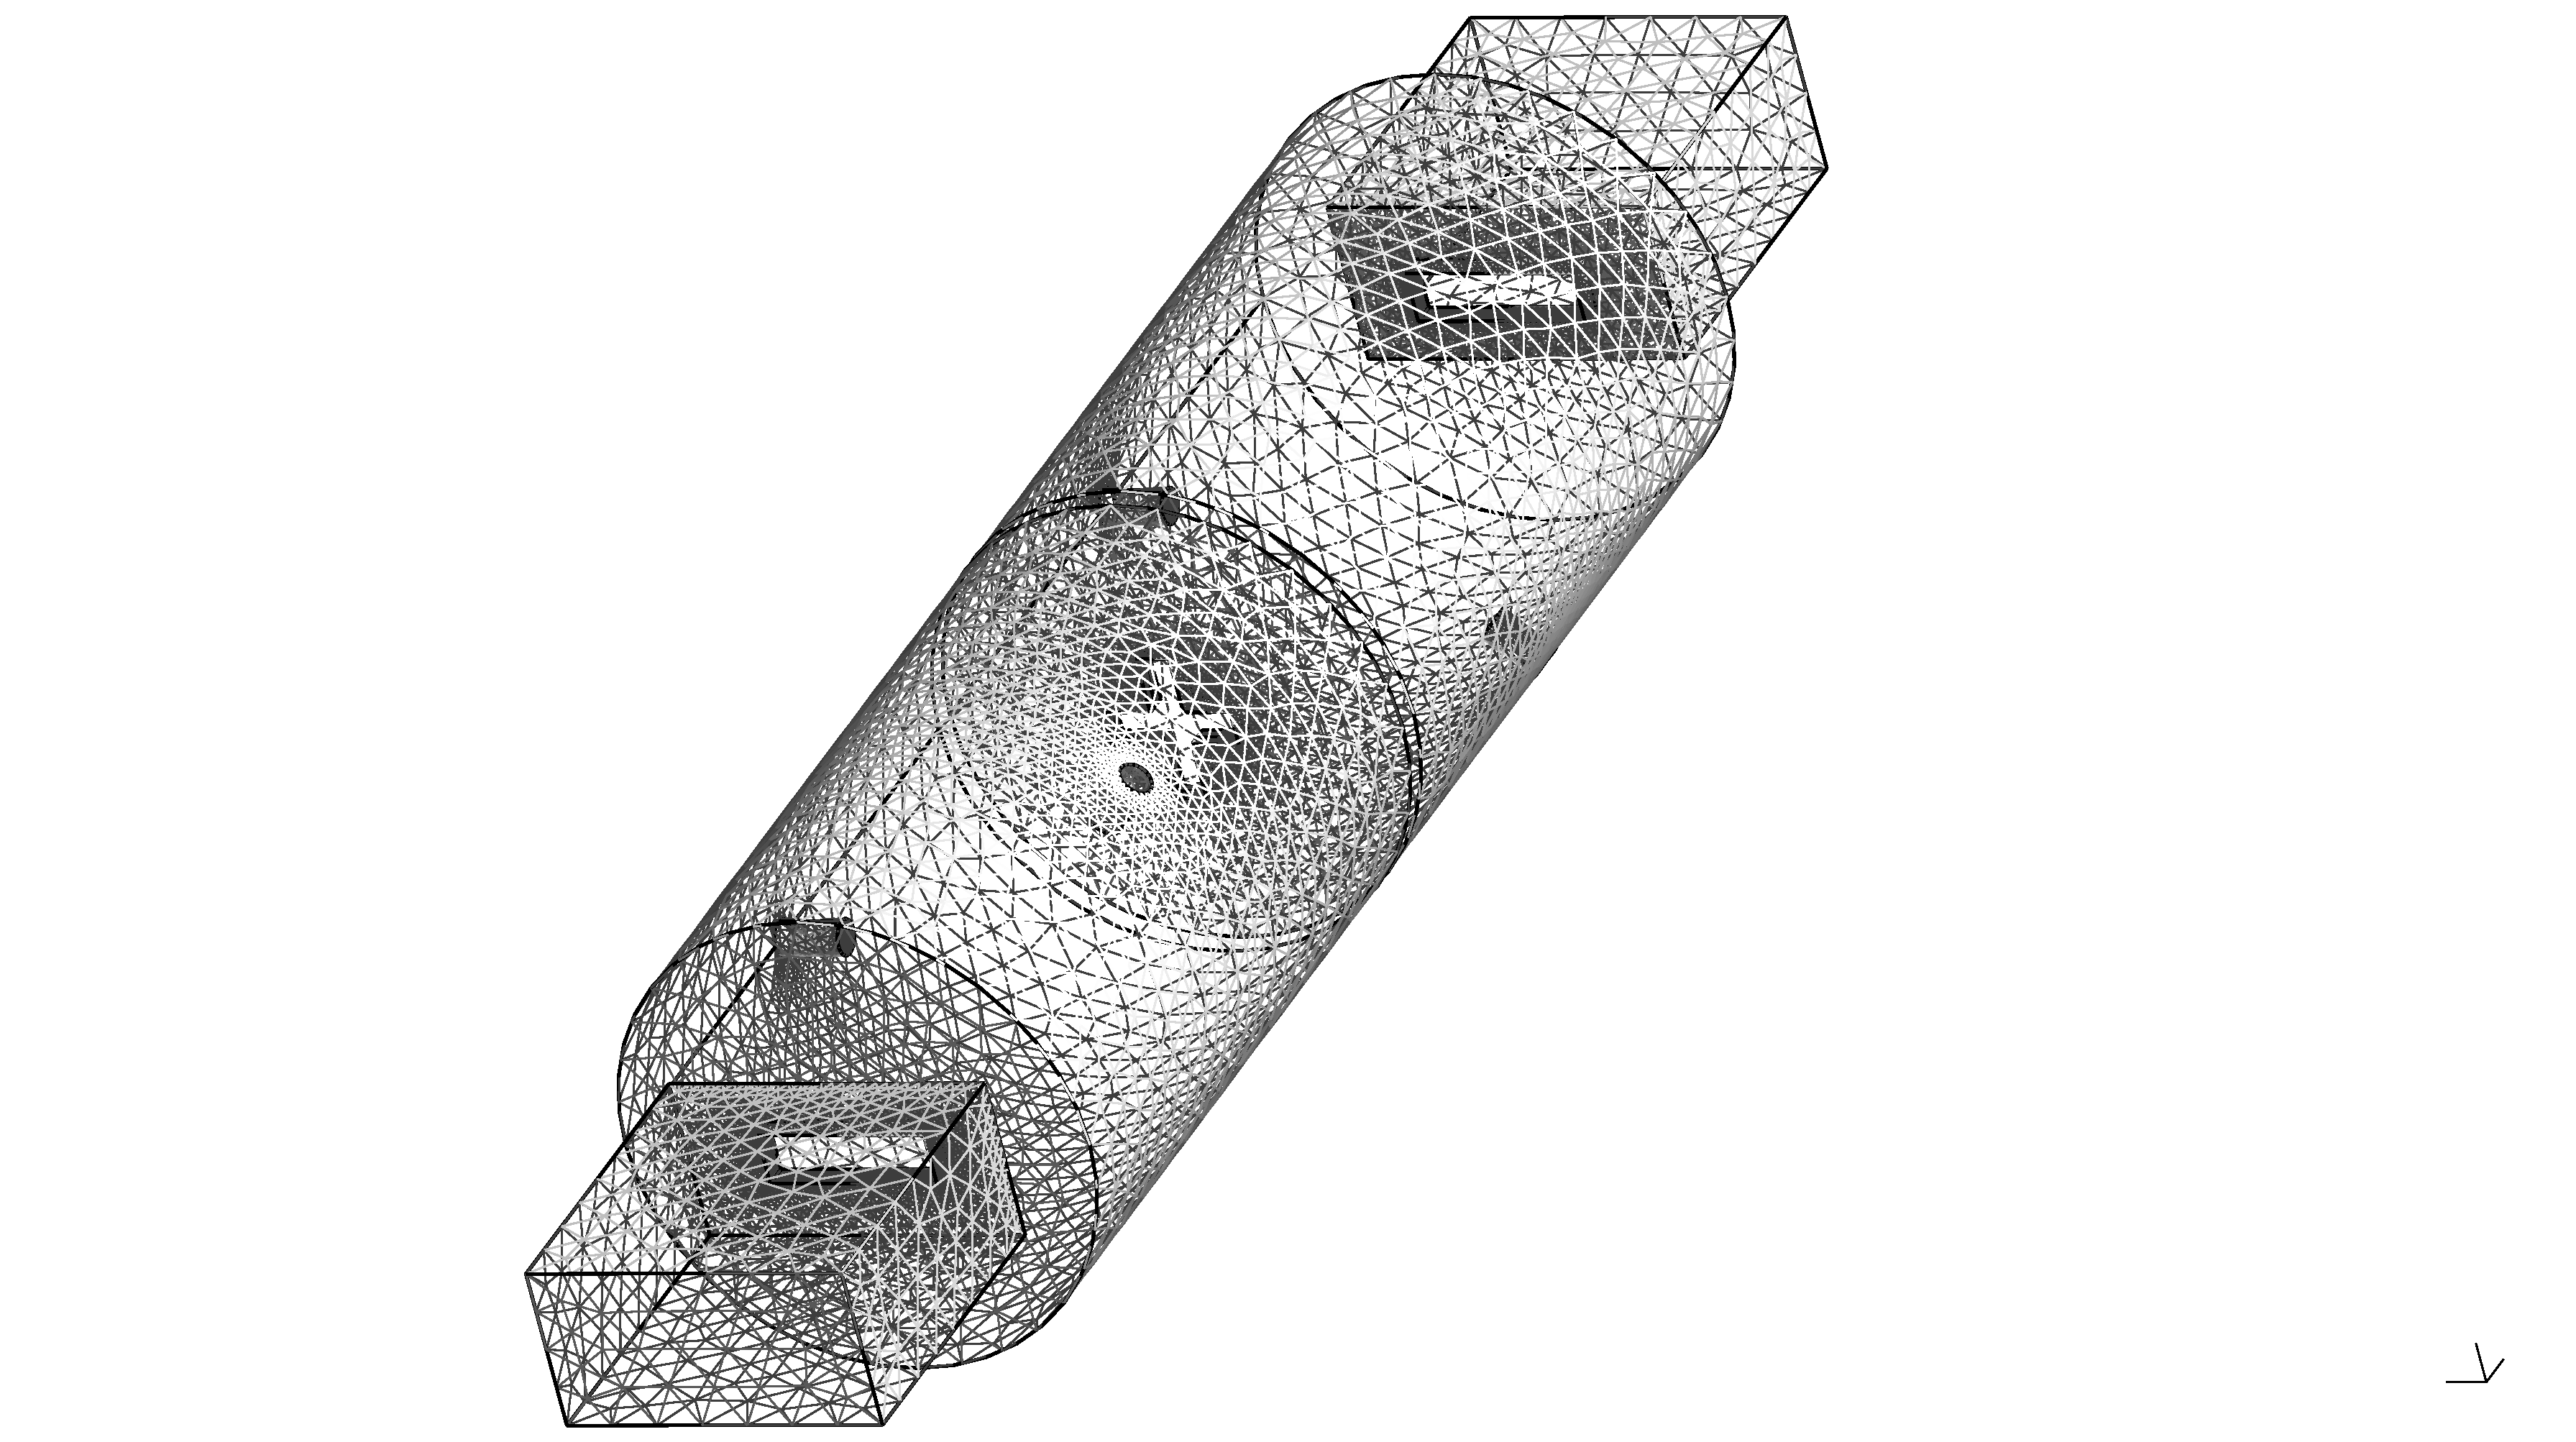
\includegraphics[scale=0.18, trim=12cm 0.2cm 15cm 0.2cm, clip]{../report/figures/DMCWF_surfacemesh.pdf}};
                \draw[thick, fill=black!5!white] (5.65, 1.9) rectangle (6.9, 3.1);
\draw[thick, fill=black!5!white] (7, 1.6) rectangle (9.75, 3.4);
\draw[thick, fill=black!5!white] (9.85, 1.6) rectangle (12.65, 3.4);
\draw[thick, fill=black!5!white] (12.75, 1.9) rectangle (14, 3.1);
\draw[thick] (6.9, 2.15) to (7, 2.15);
\draw[thick] (6.9, 2.85) to (7, 2.85);
\draw[thick] (12.65, 2.15) to (12.75, 2.15);
\draw[thick] (12.65, 2.85) to (12.75, 2.85);
\draw[thick] (9.75, 2.25) to (9.85, 2.25);
\draw[thick] (9.75, 2.75) to (9.85, 2.75);
\draw[thick] (8.37, 1.85) ellipse (0.07 and 0.04);
\draw[thick, opacity=0.2] (11.25, 1.85) ellipse (0.07 and 0.04);
\draw[thick] (8.29, 3.375) to (8.44, 3.375);
\draw[thick] (11.17, 3.375) to (11.33, 3.375);

\draw[<->] (7, 3.6) -- (9.75, 3.6) node [midway, above] {$L_C$};
\draw[<->] (5.65, 3.3) -- (6.9, 3.3) node [midway, above] {$L_B$};
\draw[<->] (5.45, 3.1) -- (5.45, 1.9) node [midway, left] {$W_B$};
\draw[<->] (7.8, 1.7) -- (7.8, 3.3) node [midway, left] {$D_C$};

\begin{scope}[shift={(0, -0.5)}]

    \draw[thick, fill=black!5!white] (6.5, 0) circle (1);
    \draw[thick, fill=black!10!white] (5.8, -0.35) rectangle (7.2, 0.35);
    \draw[thick, fill=white] (6.1, -0.083) rectangle (6.9, 0.083);

    \draw[dashed] (6.1, 0.083) to (6.1, 1.25);
    \draw[dashed] (6.9, 0.083) to (6.9, 1.25);
    \draw[<->] (6.1, 1.15) -- (6.9, 1.15) node [midway, above] {$W_S$};
    \draw[dashed] (6.1, 0.083) to (5.2, 0.083);
    \draw[dashed] (6.1, -0.083) to (5.2, -0.083);
    \draw[<->] (5.3, -0.083) -- (5.3, 0.083) node [midway, left] {$H_S$};
    \draw[dashed] (7.2, -0.35) to (7.7, -0.35);
    \draw[dashed] (7.2, 0.35) to (7.7, 0.35);
    \draw[<->] (7.6, -0.35) -- (7.6, 0.35) node [midway, right] {$H_B$};

\end{scope}

\begin{scope}[shift={(0.05, -0.5)}]

    \draw[thick, fill=black!5!white] (9.76, 0) circle (1);
    \draw[thick, fill=white] (9.68, -0.35) to (9.84, -0.35) to (9.84, -0.08) to (10.06, -0.08)
                    to (10.06, 0.08) to (9.84, 0.08) to (9.84, 0.35) to (9.68, 0.35)
                    to (9.68, 0.08) to (9.46, 0.08) to (9.46, -0.08) to (9.68, -0.08)
                    to cycle;


    \draw[dashed] (9.84, 0.35) to (9.84, 1.25);
    \draw[dashed] (9.68, 0.35) to (9.68, 1.25);
    \draw[<->] (9.68, 1.15) -- (9.84, 1.15) node [midway, above] {$W_A$};
    
    \draw[dashed] (9.68, -0.35) to (9.68, -1.25);
    \draw[dashed] (9.46, -0.083) to (9.46, -1.25);
    \draw[<->] (9.46, -1.15) -- (9.68, -1.15) node [midway, below] {$L_A$};

    %\draw[dashed] (9.46, -0.083) to (8.5, -0.083);
    %\draw[dashed] (9.46, 0.083) to (8.5, 0.083);
    %\draw[<->] (8.6, -0.083) -- (8.6, 0.083) node [midway, left] {$c$};
    
    \draw[dashed] (9.84, 0.35) to (11, 0.35);
    \draw[dashed] (10.06, 0.083) to (11, 0.083);
    \draw[<->] (10.9, 0.083) -- (10.9, 0.35) node [midway, right] {$H_A$};

\end{scope}
            \end{tikzpicture}
        }
    \end{figure}

\end{frame}

\begin{frame}{Example application 3 | Scattering coefficients}

    \begin{figure}
        \centering
        \scalebox{0.7}{%% Creator: Matplotlib, PGF backend
%%
%% To include the figure in your LaTeX document, write
%%   \input{<filename>.pgf}
%%
%% Make sure the required packages are loaded in your preamble
%%   \usepackage{pgf}
%%
%% Also ensure that all the required font packages are loaded; for instance,
%% the lmodern package is sometimes necessary when using math font.
%%   \usepackage{lmodern}
%%
%% Figures using additional raster images can only be included by \input if
%% they are in the same directory as the main LaTeX file. For loading figures
%% from other directories you can use the `import` package
%%   \usepackage{import}
%%
%% and then include the figures with
%%   \import{<path to file>}{<filename>.pgf}
%%
%% Matplotlib used the following preamble
%%   \usepackage{fontspec}
%%   \setmainfont{DejaVuSans.ttf}[Path=\detokenize{C:/Users/Fabio/Anaconda3/Lib/site-packages/matplotlib/mpl-data/fonts/ttf/}]
%%   \setsansfont{DejaVuSans.ttf}[Path=\detokenize{C:/Users/Fabio/Anaconda3/Lib/site-packages/matplotlib/mpl-data/fonts/ttf/}]
%%   \setmonofont{DejaVuSansMono.ttf}[Path=\detokenize{C:/Users/Fabio/Anaconda3/Lib/site-packages/matplotlib/mpl-data/fonts/ttf/}]
%%
\begingroup%
\makeatletter%
\begin{pgfpicture}%
\pgfpathrectangle{\pgfpointorigin}{\pgfqpoint{5.078495in}{3.668486in}}%
\pgfusepath{use as bounding box, clip}%
\begin{pgfscope}%
\pgfsetbuttcap%
\pgfsetmiterjoin%
\pgfsetlinewidth{0.000000pt}%
\definecolor{currentstroke}{rgb}{1.000000,1.000000,1.000000}%
\pgfsetstrokecolor{currentstroke}%
\pgfsetstrokeopacity{0.000000}%
\pgfsetdash{}{0pt}%
\pgfpathmoveto{\pgfqpoint{0.000000in}{0.000000in}}%
\pgfpathlineto{\pgfqpoint{5.078495in}{0.000000in}}%
\pgfpathlineto{\pgfqpoint{5.078495in}{3.668486in}}%
\pgfpathlineto{\pgfqpoint{0.000000in}{3.668486in}}%
\pgfpathlineto{\pgfqpoint{0.000000in}{0.000000in}}%
\pgfpathclose%
\pgfusepath{}%
\end{pgfscope}%
\begin{pgfscope}%
\pgfsetbuttcap%
\pgfsetmiterjoin%
\definecolor{currentfill}{rgb}{1.000000,1.000000,1.000000}%
\pgfsetfillcolor{currentfill}%
\pgfsetlinewidth{0.000000pt}%
\definecolor{currentstroke}{rgb}{0.000000,0.000000,0.000000}%
\pgfsetstrokecolor{currentstroke}%
\pgfsetstrokeopacity{0.000000}%
\pgfsetdash{}{0pt}%
\pgfpathmoveto{\pgfqpoint{0.677245in}{2.058486in}}%
\pgfpathlineto{\pgfqpoint{4.978495in}{2.058486in}}%
\pgfpathlineto{\pgfqpoint{4.978495in}{3.568486in}}%
\pgfpathlineto{\pgfqpoint{0.677245in}{3.568486in}}%
\pgfpathlineto{\pgfqpoint{0.677245in}{2.058486in}}%
\pgfpathclose%
\pgfusepath{fill}%
\end{pgfscope}%
\begin{pgfscope}%
\pgfsetbuttcap%
\pgfsetroundjoin%
\definecolor{currentfill}{rgb}{0.000000,0.000000,0.000000}%
\pgfsetfillcolor{currentfill}%
\pgfsetlinewidth{0.803000pt}%
\definecolor{currentstroke}{rgb}{0.000000,0.000000,0.000000}%
\pgfsetstrokecolor{currentstroke}%
\pgfsetdash{}{0pt}%
\pgfsys@defobject{currentmarker}{\pgfqpoint{0.000000in}{-0.048611in}}{\pgfqpoint{0.000000in}{0.000000in}}{%
\pgfpathmoveto{\pgfqpoint{0.000000in}{0.000000in}}%
\pgfpathlineto{\pgfqpoint{0.000000in}{-0.048611in}}%
\pgfusepath{stroke,fill}%
}%
\begin{pgfscope}%
\pgfsys@transformshift{1.411800in}{2.058486in}%
\pgfsys@useobject{currentmarker}{}%
\end{pgfscope}%
\end{pgfscope}%
\begin{pgfscope}%
\pgfsetbuttcap%
\pgfsetroundjoin%
\definecolor{currentfill}{rgb}{0.000000,0.000000,0.000000}%
\pgfsetfillcolor{currentfill}%
\pgfsetlinewidth{0.803000pt}%
\definecolor{currentstroke}{rgb}{0.000000,0.000000,0.000000}%
\pgfsetstrokecolor{currentstroke}%
\pgfsetdash{}{0pt}%
\pgfsys@defobject{currentmarker}{\pgfqpoint{0.000000in}{-0.048611in}}{\pgfqpoint{0.000000in}{0.000000in}}{%
\pgfpathmoveto{\pgfqpoint{0.000000in}{0.000000in}}%
\pgfpathlineto{\pgfqpoint{0.000000in}{-0.048611in}}%
\pgfusepath{stroke,fill}%
}%
\begin{pgfscope}%
\pgfsys@transformshift{2.267506in}{2.058486in}%
\pgfsys@useobject{currentmarker}{}%
\end{pgfscope}%
\end{pgfscope}%
\begin{pgfscope}%
\pgfsetbuttcap%
\pgfsetroundjoin%
\definecolor{currentfill}{rgb}{0.000000,0.000000,0.000000}%
\pgfsetfillcolor{currentfill}%
\pgfsetlinewidth{0.803000pt}%
\definecolor{currentstroke}{rgb}{0.000000,0.000000,0.000000}%
\pgfsetstrokecolor{currentstroke}%
\pgfsetdash{}{0pt}%
\pgfsys@defobject{currentmarker}{\pgfqpoint{0.000000in}{-0.048611in}}{\pgfqpoint{0.000000in}{0.000000in}}{%
\pgfpathmoveto{\pgfqpoint{0.000000in}{0.000000in}}%
\pgfpathlineto{\pgfqpoint{0.000000in}{-0.048611in}}%
\pgfusepath{stroke,fill}%
}%
\begin{pgfscope}%
\pgfsys@transformshift{3.123213in}{2.058486in}%
\pgfsys@useobject{currentmarker}{}%
\end{pgfscope}%
\end{pgfscope}%
\begin{pgfscope}%
\pgfsetbuttcap%
\pgfsetroundjoin%
\definecolor{currentfill}{rgb}{0.000000,0.000000,0.000000}%
\pgfsetfillcolor{currentfill}%
\pgfsetlinewidth{0.803000pt}%
\definecolor{currentstroke}{rgb}{0.000000,0.000000,0.000000}%
\pgfsetstrokecolor{currentstroke}%
\pgfsetdash{}{0pt}%
\pgfsys@defobject{currentmarker}{\pgfqpoint{0.000000in}{-0.048611in}}{\pgfqpoint{0.000000in}{0.000000in}}{%
\pgfpathmoveto{\pgfqpoint{0.000000in}{0.000000in}}%
\pgfpathlineto{\pgfqpoint{0.000000in}{-0.048611in}}%
\pgfusepath{stroke,fill}%
}%
\begin{pgfscope}%
\pgfsys@transformshift{3.978919in}{2.058486in}%
\pgfsys@useobject{currentmarker}{}%
\end{pgfscope}%
\end{pgfscope}%
\begin{pgfscope}%
\pgfsetbuttcap%
\pgfsetroundjoin%
\definecolor{currentfill}{rgb}{0.000000,0.000000,0.000000}%
\pgfsetfillcolor{currentfill}%
\pgfsetlinewidth{0.803000pt}%
\definecolor{currentstroke}{rgb}{0.000000,0.000000,0.000000}%
\pgfsetstrokecolor{currentstroke}%
\pgfsetdash{}{0pt}%
\pgfsys@defobject{currentmarker}{\pgfqpoint{0.000000in}{-0.048611in}}{\pgfqpoint{0.000000in}{0.000000in}}{%
\pgfpathmoveto{\pgfqpoint{0.000000in}{0.000000in}}%
\pgfpathlineto{\pgfqpoint{0.000000in}{-0.048611in}}%
\pgfusepath{stroke,fill}%
}%
\begin{pgfscope}%
\pgfsys@transformshift{4.834626in}{2.058486in}%
\pgfsys@useobject{currentmarker}{}%
\end{pgfscope}%
\end{pgfscope}%
\begin{pgfscope}%
\pgfpathrectangle{\pgfqpoint{0.677245in}{2.058486in}}{\pgfqpoint{4.301250in}{1.510000in}}%
\pgfusepath{clip}%
\pgfsetrectcap%
\pgfsetroundjoin%
\pgfsetlinewidth{0.803000pt}%
\definecolor{currentstroke}{rgb}{0.690196,0.690196,0.690196}%
\pgfsetstrokecolor{currentstroke}%
\pgfsetdash{}{0pt}%
\pgfpathmoveto{\pgfqpoint{0.677245in}{2.416736in}}%
\pgfpathlineto{\pgfqpoint{4.978495in}{2.416736in}}%
\pgfusepath{stroke}%
\end{pgfscope}%
\begin{pgfscope}%
\pgfsetbuttcap%
\pgfsetroundjoin%
\definecolor{currentfill}{rgb}{0.000000,0.000000,0.000000}%
\pgfsetfillcolor{currentfill}%
\pgfsetlinewidth{0.803000pt}%
\definecolor{currentstroke}{rgb}{0.000000,0.000000,0.000000}%
\pgfsetstrokecolor{currentstroke}%
\pgfsetdash{}{0pt}%
\pgfsys@defobject{currentmarker}{\pgfqpoint{-0.048611in}{0.000000in}}{\pgfqpoint{-0.000000in}{0.000000in}}{%
\pgfpathmoveto{\pgfqpoint{-0.000000in}{0.000000in}}%
\pgfpathlineto{\pgfqpoint{-0.048611in}{0.000000in}}%
\pgfusepath{stroke,fill}%
}%
\begin{pgfscope}%
\pgfsys@transformshift{0.677245in}{2.416736in}%
\pgfsys@useobject{currentmarker}{}%
\end{pgfscope}%
\end{pgfscope}%
\begin{pgfscope}%
\definecolor{textcolor}{rgb}{0.000000,0.000000,0.000000}%
\pgfsetstrokecolor{textcolor}%
\pgfsetfillcolor{textcolor}%
\pgftext[x=0.309652in, y=2.358699in, left, base]{\color{textcolor}\rmfamily\fontsize{11.000000}{13.200000}\selectfont \(\displaystyle {\ensuremath{-}40}\)}%
\end{pgfscope}%
\begin{pgfscope}%
\pgfpathrectangle{\pgfqpoint{0.677245in}{2.058486in}}{\pgfqpoint{4.301250in}{1.510000in}}%
\pgfusepath{clip}%
\pgfsetrectcap%
\pgfsetroundjoin%
\pgfsetlinewidth{0.803000pt}%
\definecolor{currentstroke}{rgb}{0.690196,0.690196,0.690196}%
\pgfsetstrokecolor{currentstroke}%
\pgfsetdash{}{0pt}%
\pgfpathmoveto{\pgfqpoint{0.677245in}{2.958293in}}%
\pgfpathlineto{\pgfqpoint{4.978495in}{2.958293in}}%
\pgfusepath{stroke}%
\end{pgfscope}%
\begin{pgfscope}%
\pgfsetbuttcap%
\pgfsetroundjoin%
\definecolor{currentfill}{rgb}{0.000000,0.000000,0.000000}%
\pgfsetfillcolor{currentfill}%
\pgfsetlinewidth{0.803000pt}%
\definecolor{currentstroke}{rgb}{0.000000,0.000000,0.000000}%
\pgfsetstrokecolor{currentstroke}%
\pgfsetdash{}{0pt}%
\pgfsys@defobject{currentmarker}{\pgfqpoint{-0.048611in}{0.000000in}}{\pgfqpoint{-0.000000in}{0.000000in}}{%
\pgfpathmoveto{\pgfqpoint{-0.000000in}{0.000000in}}%
\pgfpathlineto{\pgfqpoint{-0.048611in}{0.000000in}}%
\pgfusepath{stroke,fill}%
}%
\begin{pgfscope}%
\pgfsys@transformshift{0.677245in}{2.958293in}%
\pgfsys@useobject{currentmarker}{}%
\end{pgfscope}%
\end{pgfscope}%
\begin{pgfscope}%
\definecolor{textcolor}{rgb}{0.000000,0.000000,0.000000}%
\pgfsetstrokecolor{textcolor}%
\pgfsetfillcolor{textcolor}%
\pgftext[x=0.309652in, y=2.900255in, left, base]{\color{textcolor}\rmfamily\fontsize{11.000000}{13.200000}\selectfont \(\displaystyle {\ensuremath{-}20}\)}%
\end{pgfscope}%
\begin{pgfscope}%
\pgfpathrectangle{\pgfqpoint{0.677245in}{2.058486in}}{\pgfqpoint{4.301250in}{1.510000in}}%
\pgfusepath{clip}%
\pgfsetrectcap%
\pgfsetroundjoin%
\pgfsetlinewidth{0.803000pt}%
\definecolor{currentstroke}{rgb}{0.690196,0.690196,0.690196}%
\pgfsetstrokecolor{currentstroke}%
\pgfsetdash{}{0pt}%
\pgfpathmoveto{\pgfqpoint{0.677245in}{3.499849in}}%
\pgfpathlineto{\pgfqpoint{4.978495in}{3.499849in}}%
\pgfusepath{stroke}%
\end{pgfscope}%
\begin{pgfscope}%
\pgfsetbuttcap%
\pgfsetroundjoin%
\definecolor{currentfill}{rgb}{0.000000,0.000000,0.000000}%
\pgfsetfillcolor{currentfill}%
\pgfsetlinewidth{0.803000pt}%
\definecolor{currentstroke}{rgb}{0.000000,0.000000,0.000000}%
\pgfsetstrokecolor{currentstroke}%
\pgfsetdash{}{0pt}%
\pgfsys@defobject{currentmarker}{\pgfqpoint{-0.048611in}{0.000000in}}{\pgfqpoint{-0.000000in}{0.000000in}}{%
\pgfpathmoveto{\pgfqpoint{-0.000000in}{0.000000in}}%
\pgfpathlineto{\pgfqpoint{-0.048611in}{0.000000in}}%
\pgfusepath{stroke,fill}%
}%
\begin{pgfscope}%
\pgfsys@transformshift{0.677245in}{3.499849in}%
\pgfsys@useobject{currentmarker}{}%
\end{pgfscope}%
\end{pgfscope}%
\begin{pgfscope}%
\definecolor{textcolor}{rgb}{0.000000,0.000000,0.000000}%
\pgfsetstrokecolor{textcolor}%
\pgfsetfillcolor{textcolor}%
\pgftext[x=0.503981in, y=3.441812in, left, base]{\color{textcolor}\rmfamily\fontsize{11.000000}{13.200000}\selectfont \(\displaystyle {0}\)}%
\end{pgfscope}%
\begin{pgfscope}%
\definecolor{textcolor}{rgb}{0.000000,0.000000,0.000000}%
\pgfsetstrokecolor{textcolor}%
\pgfsetfillcolor{textcolor}%
\pgftext[x=0.254096in,y=2.813486in,,bottom,rotate=90.000000]{\color{textcolor}\rmfamily\fontsize{11.000000}{13.200000}\selectfont \(\displaystyle S_{11}(\omega)\) (dB)}%
\end{pgfscope}%
\begin{pgfscope}%
\pgfpathrectangle{\pgfqpoint{0.677245in}{2.058486in}}{\pgfqpoint{4.301250in}{1.510000in}}%
\pgfusepath{clip}%
\pgfsetrectcap%
\pgfsetroundjoin%
\pgfsetlinewidth{1.505625pt}%
\definecolor{currentstroke}{rgb}{0.001462,0.000466,0.013866}%
\pgfsetstrokecolor{currentstroke}%
\pgfsetdash{}{0pt}%
\pgfpathmoveto{\pgfqpoint{0.677245in}{3.498630in}}%
\pgfpathlineto{\pgfqpoint{1.803075in}{3.496865in}}%
\pgfpathlineto{\pgfqpoint{1.976280in}{3.499849in}}%
\pgfpathlineto{\pgfqpoint{2.034015in}{3.497600in}}%
\pgfpathlineto{\pgfqpoint{2.062882in}{3.493945in}}%
\pgfpathlineto{\pgfqpoint{2.091750in}{3.486979in}}%
\pgfpathlineto{\pgfqpoint{2.120617in}{3.474489in}}%
\pgfpathlineto{\pgfqpoint{2.149485in}{3.452864in}}%
\pgfpathlineto{\pgfqpoint{2.178352in}{3.416462in}}%
\pgfpathlineto{\pgfqpoint{2.207219in}{3.356865in}}%
\pgfpathlineto{\pgfqpoint{2.236087in}{3.262664in}}%
\pgfpathlineto{\pgfqpoint{2.264954in}{3.118970in}}%
\pgfpathlineto{\pgfqpoint{2.293822in}{2.904230in}}%
\pgfpathlineto{\pgfqpoint{2.322689in}{2.574688in}}%
\pgfpathlineto{\pgfqpoint{2.351557in}{2.127122in}}%
\pgfpathlineto{\pgfqpoint{2.380424in}{2.353954in}}%
\pgfpathlineto{\pgfqpoint{2.409292in}{2.635869in}}%
\pgfpathlineto{\pgfqpoint{2.438159in}{2.797759in}}%
\pgfpathlineto{\pgfqpoint{2.467026in}{2.900111in}}%
\pgfpathlineto{\pgfqpoint{2.495894in}{2.969325in}}%
\pgfpathlineto{\pgfqpoint{2.524761in}{3.018407in}}%
\pgfpathlineto{\pgfqpoint{2.553629in}{3.053946in}}%
\pgfpathlineto{\pgfqpoint{2.582496in}{3.080155in}}%
\pgfpathlineto{\pgfqpoint{2.611364in}{3.099255in}}%
\pgfpathlineto{\pgfqpoint{2.640231in}{3.113016in}}%
\pgfpathlineto{\pgfqpoint{2.669099in}{3.122227in}}%
\pgfpathlineto{\pgfqpoint{2.697966in}{3.127715in}}%
\pgfpathlineto{\pgfqpoint{2.726834in}{3.129637in}}%
\pgfpathlineto{\pgfqpoint{2.755701in}{3.128331in}}%
\pgfpathlineto{\pgfqpoint{2.784568in}{3.123556in}}%
\pgfpathlineto{\pgfqpoint{2.813436in}{3.115261in}}%
\pgfpathlineto{\pgfqpoint{2.842303in}{3.102796in}}%
\pgfpathlineto{\pgfqpoint{2.871171in}{3.085606in}}%
\pgfpathlineto{\pgfqpoint{2.900038in}{3.062380in}}%
\pgfpathlineto{\pgfqpoint{2.928906in}{3.031606in}}%
\pgfpathlineto{\pgfqpoint{2.957773in}{2.990527in}}%
\pgfpathlineto{\pgfqpoint{2.986641in}{2.935315in}}%
\pgfpathlineto{\pgfqpoint{3.015508in}{2.859337in}}%
\pgfpathlineto{\pgfqpoint{3.044375in}{2.752175in}}%
\pgfpathlineto{\pgfqpoint{3.073243in}{2.598180in}}%
\pgfpathlineto{\pgfqpoint{3.102110in}{2.406507in}}%
\pgfpathlineto{\pgfqpoint{3.130978in}{2.403647in}}%
\pgfpathlineto{\pgfqpoint{3.159845in}{2.665074in}}%
\pgfpathlineto{\pgfqpoint{3.188713in}{2.906353in}}%
\pgfpathlineto{\pgfqpoint{3.217580in}{3.085759in}}%
\pgfpathlineto{\pgfqpoint{3.246448in}{3.215996in}}%
\pgfpathlineto{\pgfqpoint{3.275315in}{3.308939in}}%
\pgfpathlineto{\pgfqpoint{3.304183in}{3.373705in}}%
\pgfpathlineto{\pgfqpoint{3.333050in}{3.417910in}}%
\pgfpathlineto{\pgfqpoint{3.361917in}{3.447524in}}%
\pgfpathlineto{\pgfqpoint{3.390785in}{3.467123in}}%
\pgfpathlineto{\pgfqpoint{3.419652in}{3.479931in}}%
\pgfpathlineto{\pgfqpoint{3.448520in}{3.488200in}}%
\pgfpathlineto{\pgfqpoint{3.477387in}{3.493434in}}%
\pgfpathlineto{\pgfqpoint{3.535122in}{3.498510in}}%
\pgfpathlineto{\pgfqpoint{3.592857in}{3.499844in}}%
\pgfpathlineto{\pgfqpoint{3.708327in}{3.498590in}}%
\pgfpathlineto{\pgfqpoint{4.083604in}{3.492401in}}%
\pgfpathlineto{\pgfqpoint{4.430013in}{3.490532in}}%
\pgfpathlineto{\pgfqpoint{4.978495in}{3.491037in}}%
\pgfpathlineto{\pgfqpoint{4.978495in}{3.491037in}}%
\pgfusepath{stroke}%
\end{pgfscope}%
\begin{pgfscope}%
\pgfpathrectangle{\pgfqpoint{0.677245in}{2.058486in}}{\pgfqpoint{4.301250in}{1.510000in}}%
\pgfusepath{clip}%
\pgfsetrectcap%
\pgfsetroundjoin%
\pgfsetlinewidth{1.505625pt}%
\definecolor{currentstroke}{rgb}{0.735683,0.215906,0.330245}%
\pgfsetstrokecolor{currentstroke}%
\pgfsetdash{}{0pt}%
\pgfpathmoveto{\pgfqpoint{0.677245in}{3.498630in}}%
\pgfpathlineto{\pgfqpoint{1.803075in}{3.496865in}}%
\pgfpathlineto{\pgfqpoint{1.976280in}{3.499849in}}%
\pgfpathlineto{\pgfqpoint{2.034015in}{3.497600in}}%
\pgfpathlineto{\pgfqpoint{2.062882in}{3.493945in}}%
\pgfpathlineto{\pgfqpoint{2.091750in}{3.486979in}}%
\pgfpathlineto{\pgfqpoint{2.120617in}{3.474489in}}%
\pgfpathlineto{\pgfqpoint{2.149485in}{3.452864in}}%
\pgfpathlineto{\pgfqpoint{2.178352in}{3.416462in}}%
\pgfpathlineto{\pgfqpoint{2.207219in}{3.356865in}}%
\pgfpathlineto{\pgfqpoint{2.236087in}{3.262663in}}%
\pgfpathlineto{\pgfqpoint{2.264954in}{3.118969in}}%
\pgfpathlineto{\pgfqpoint{2.293822in}{2.904229in}}%
\pgfpathlineto{\pgfqpoint{2.322689in}{2.574685in}}%
\pgfpathlineto{\pgfqpoint{2.351557in}{2.127122in}}%
\pgfpathlineto{\pgfqpoint{2.380424in}{2.353959in}}%
\pgfpathlineto{\pgfqpoint{2.409292in}{2.635872in}}%
\pgfpathlineto{\pgfqpoint{2.438159in}{2.797761in}}%
\pgfpathlineto{\pgfqpoint{2.467026in}{2.900113in}}%
\pgfpathlineto{\pgfqpoint{2.495894in}{2.969326in}}%
\pgfpathlineto{\pgfqpoint{2.524761in}{3.018408in}}%
\pgfpathlineto{\pgfqpoint{2.553629in}{3.053948in}}%
\pgfpathlineto{\pgfqpoint{2.582496in}{3.080156in}}%
\pgfpathlineto{\pgfqpoint{2.611364in}{3.099256in}}%
\pgfpathlineto{\pgfqpoint{2.640231in}{3.113017in}}%
\pgfpathlineto{\pgfqpoint{2.669099in}{3.122228in}}%
\pgfpathlineto{\pgfqpoint{2.697966in}{3.127716in}}%
\pgfpathlineto{\pgfqpoint{2.726834in}{3.129638in}}%
\pgfpathlineto{\pgfqpoint{2.755701in}{3.128332in}}%
\pgfpathlineto{\pgfqpoint{2.784568in}{3.123557in}}%
\pgfpathlineto{\pgfqpoint{2.813436in}{3.115262in}}%
\pgfpathlineto{\pgfqpoint{2.842303in}{3.102797in}}%
\pgfpathlineto{\pgfqpoint{2.871171in}{3.085607in}}%
\pgfpathlineto{\pgfqpoint{2.900038in}{3.062381in}}%
\pgfpathlineto{\pgfqpoint{2.928906in}{3.031607in}}%
\pgfpathlineto{\pgfqpoint{2.957773in}{2.990528in}}%
\pgfpathlineto{\pgfqpoint{2.986641in}{2.935316in}}%
\pgfpathlineto{\pgfqpoint{3.015508in}{2.859338in}}%
\pgfpathlineto{\pgfqpoint{3.044375in}{2.752175in}}%
\pgfpathlineto{\pgfqpoint{3.073243in}{2.598181in}}%
\pgfpathlineto{\pgfqpoint{3.102110in}{2.406507in}}%
\pgfpathlineto{\pgfqpoint{3.130978in}{2.403647in}}%
\pgfpathlineto{\pgfqpoint{3.159845in}{2.665074in}}%
\pgfpathlineto{\pgfqpoint{3.188713in}{2.906353in}}%
\pgfpathlineto{\pgfqpoint{3.217580in}{3.085759in}}%
\pgfpathlineto{\pgfqpoint{3.246448in}{3.215996in}}%
\pgfpathlineto{\pgfqpoint{3.275315in}{3.308939in}}%
\pgfpathlineto{\pgfqpoint{3.304183in}{3.373705in}}%
\pgfpathlineto{\pgfqpoint{3.333050in}{3.417910in}}%
\pgfpathlineto{\pgfqpoint{3.361917in}{3.447524in}}%
\pgfpathlineto{\pgfqpoint{3.390785in}{3.467123in}}%
\pgfpathlineto{\pgfqpoint{3.419652in}{3.479931in}}%
\pgfpathlineto{\pgfqpoint{3.448520in}{3.488200in}}%
\pgfpathlineto{\pgfqpoint{3.477387in}{3.493434in}}%
\pgfpathlineto{\pgfqpoint{3.535122in}{3.498510in}}%
\pgfpathlineto{\pgfqpoint{3.592857in}{3.499844in}}%
\pgfpathlineto{\pgfqpoint{3.708327in}{3.498590in}}%
\pgfpathlineto{\pgfqpoint{4.083604in}{3.492399in}}%
\pgfpathlineto{\pgfqpoint{4.430013in}{3.490529in}}%
\pgfpathlineto{\pgfqpoint{4.978495in}{3.491037in}}%
\pgfpathlineto{\pgfqpoint{4.978495in}{3.491037in}}%
\pgfusepath{stroke}%
\end{pgfscope}%
\begin{pgfscope}%
\pgfsetrectcap%
\pgfsetmiterjoin%
\pgfsetlinewidth{0.803000pt}%
\definecolor{currentstroke}{rgb}{0.000000,0.000000,0.000000}%
\pgfsetstrokecolor{currentstroke}%
\pgfsetdash{}{0pt}%
\pgfpathmoveto{\pgfqpoint{0.677245in}{2.058486in}}%
\pgfpathlineto{\pgfqpoint{0.677245in}{3.568486in}}%
\pgfusepath{stroke}%
\end{pgfscope}%
\begin{pgfscope}%
\pgfsetrectcap%
\pgfsetmiterjoin%
\pgfsetlinewidth{0.803000pt}%
\definecolor{currentstroke}{rgb}{0.000000,0.000000,0.000000}%
\pgfsetstrokecolor{currentstroke}%
\pgfsetdash{}{0pt}%
\pgfpathmoveto{\pgfqpoint{4.978495in}{2.058486in}}%
\pgfpathlineto{\pgfqpoint{4.978495in}{3.568486in}}%
\pgfusepath{stroke}%
\end{pgfscope}%
\begin{pgfscope}%
\pgfsetrectcap%
\pgfsetmiterjoin%
\pgfsetlinewidth{0.803000pt}%
\definecolor{currentstroke}{rgb}{0.000000,0.000000,0.000000}%
\pgfsetstrokecolor{currentstroke}%
\pgfsetdash{}{0pt}%
\pgfpathmoveto{\pgfqpoint{0.677245in}{2.058486in}}%
\pgfpathlineto{\pgfqpoint{4.978495in}{2.058486in}}%
\pgfusepath{stroke}%
\end{pgfscope}%
\begin{pgfscope}%
\pgfsetrectcap%
\pgfsetmiterjoin%
\pgfsetlinewidth{0.803000pt}%
\definecolor{currentstroke}{rgb}{0.000000,0.000000,0.000000}%
\pgfsetstrokecolor{currentstroke}%
\pgfsetdash{}{0pt}%
\pgfpathmoveto{\pgfqpoint{0.677245in}{3.568486in}}%
\pgfpathlineto{\pgfqpoint{4.978495in}{3.568486in}}%
\pgfusepath{stroke}%
\end{pgfscope}%
\begin{pgfscope}%
\pgfsetbuttcap%
\pgfsetmiterjoin%
\definecolor{currentfill}{rgb}{1.000000,1.000000,1.000000}%
\pgfsetfillcolor{currentfill}%
\pgfsetfillopacity{0.800000}%
\pgfsetlinewidth{1.003750pt}%
\definecolor{currentstroke}{rgb}{0.800000,0.800000,0.800000}%
\pgfsetstrokecolor{currentstroke}%
\pgfsetstrokeopacity{0.800000}%
\pgfsetdash{}{0pt}%
\pgfpathmoveto{\pgfqpoint{3.653162in}{2.134875in}}%
\pgfpathlineto{\pgfqpoint{4.871550in}{2.134875in}}%
\pgfpathquadraticcurveto{\pgfqpoint{4.902106in}{2.134875in}}{\pgfqpoint{4.902106in}{2.165430in}}%
\pgfpathlineto{\pgfqpoint{4.902106in}{2.598638in}}%
\pgfpathquadraticcurveto{\pgfqpoint{4.902106in}{2.629194in}}{\pgfqpoint{4.871550in}{2.629194in}}%
\pgfpathlineto{\pgfqpoint{3.653162in}{2.629194in}}%
\pgfpathquadraticcurveto{\pgfqpoint{3.622607in}{2.629194in}}{\pgfqpoint{3.622607in}{2.598638in}}%
\pgfpathlineto{\pgfqpoint{3.622607in}{2.165430in}}%
\pgfpathquadraticcurveto{\pgfqpoint{3.622607in}{2.134875in}}{\pgfqpoint{3.653162in}{2.134875in}}%
\pgfpathlineto{\pgfqpoint{3.653162in}{2.134875in}}%
\pgfpathclose%
\pgfusepath{stroke,fill}%
\end{pgfscope}%
\begin{pgfscope}%
\pgfsetrectcap%
\pgfsetroundjoin%
\pgfsetlinewidth{1.505625pt}%
\definecolor{currentstroke}{rgb}{0.001462,0.000466,0.013866}%
\pgfsetstrokecolor{currentstroke}%
\pgfsetdash{}{0pt}%
\pgfpathmoveto{\pgfqpoint{3.683718in}{2.505480in}}%
\pgfpathlineto{\pgfqpoint{3.836496in}{2.505480in}}%
\pgfpathlineto{\pgfqpoint{3.989273in}{2.505480in}}%
\pgfusepath{stroke}%
\end{pgfscope}%
\begin{pgfscope}%
\definecolor{textcolor}{rgb}{0.000000,0.000000,0.000000}%
\pgfsetstrokecolor{textcolor}%
\pgfsetfillcolor{textcolor}%
\pgftext[x=4.111496in,y=2.452007in,left,base]{\color{textcolor}\rmfamily\fontsize{11.000000}{13.200000}\selectfont reference}%
\end{pgfscope}%
\begin{pgfscope}%
\pgfsetrectcap%
\pgfsetroundjoin%
\pgfsetlinewidth{1.505625pt}%
\definecolor{currentstroke}{rgb}{0.735683,0.215906,0.330245}%
\pgfsetstrokecolor{currentstroke}%
\pgfsetdash{}{0pt}%
\pgfpathmoveto{\pgfqpoint{3.683718in}{2.281237in}}%
\pgfpathlineto{\pgfqpoint{3.836496in}{2.281237in}}%
\pgfpathlineto{\pgfqpoint{3.989273in}{2.281237in}}%
\pgfusepath{stroke}%
\end{pgfscope}%
\begin{pgfscope}%
\definecolor{textcolor}{rgb}{0.000000,0.000000,0.000000}%
\pgfsetstrokecolor{textcolor}%
\pgfsetfillcolor{textcolor}%
\pgftext[x=4.111496in,y=2.227765in,left,base]{\color{textcolor}\rmfamily\fontsize{11.000000}{13.200000}\selectfont gMRI}%
\end{pgfscope}%
\begin{pgfscope}%
\pgfsetbuttcap%
\pgfsetmiterjoin%
\definecolor{currentfill}{rgb}{1.000000,1.000000,1.000000}%
\pgfsetfillcolor{currentfill}%
\pgfsetlinewidth{0.000000pt}%
\definecolor{currentstroke}{rgb}{0.000000,0.000000,0.000000}%
\pgfsetstrokecolor{currentstroke}%
\pgfsetstrokeopacity{0.000000}%
\pgfsetdash{}{0pt}%
\pgfpathmoveto{\pgfqpoint{0.677245in}{0.548486in}}%
\pgfpathlineto{\pgfqpoint{4.978495in}{0.548486in}}%
\pgfpathlineto{\pgfqpoint{4.978495in}{2.058486in}}%
\pgfpathlineto{\pgfqpoint{0.677245in}{2.058486in}}%
\pgfpathlineto{\pgfqpoint{0.677245in}{0.548486in}}%
\pgfpathclose%
\pgfusepath{fill}%
\end{pgfscope}%
\begin{pgfscope}%
\pgfsetbuttcap%
\pgfsetroundjoin%
\definecolor{currentfill}{rgb}{0.000000,0.000000,0.000000}%
\pgfsetfillcolor{currentfill}%
\pgfsetlinewidth{0.803000pt}%
\definecolor{currentstroke}{rgb}{0.000000,0.000000,0.000000}%
\pgfsetstrokecolor{currentstroke}%
\pgfsetdash{}{0pt}%
\pgfsys@defobject{currentmarker}{\pgfqpoint{0.000000in}{-0.048611in}}{\pgfqpoint{0.000000in}{0.000000in}}{%
\pgfpathmoveto{\pgfqpoint{0.000000in}{0.000000in}}%
\pgfpathlineto{\pgfqpoint{0.000000in}{-0.048611in}}%
\pgfusepath{stroke,fill}%
}%
\begin{pgfscope}%
\pgfsys@transformshift{1.411800in}{0.548486in}%
\pgfsys@useobject{currentmarker}{}%
\end{pgfscope}%
\end{pgfscope}%
\begin{pgfscope}%
\definecolor{textcolor}{rgb}{0.000000,0.000000,0.000000}%
\pgfsetstrokecolor{textcolor}%
\pgfsetfillcolor{textcolor}%
\pgftext[x=1.411800in,y=0.451264in,,top]{\color{textcolor}\rmfamily\fontsize{11.000000}{13.200000}\selectfont \(\displaystyle {7.30}\)}%
\end{pgfscope}%
\begin{pgfscope}%
\pgfsetbuttcap%
\pgfsetroundjoin%
\definecolor{currentfill}{rgb}{0.000000,0.000000,0.000000}%
\pgfsetfillcolor{currentfill}%
\pgfsetlinewidth{0.803000pt}%
\definecolor{currentstroke}{rgb}{0.000000,0.000000,0.000000}%
\pgfsetstrokecolor{currentstroke}%
\pgfsetdash{}{0pt}%
\pgfsys@defobject{currentmarker}{\pgfqpoint{0.000000in}{-0.048611in}}{\pgfqpoint{0.000000in}{0.000000in}}{%
\pgfpathmoveto{\pgfqpoint{0.000000in}{0.000000in}}%
\pgfpathlineto{\pgfqpoint{0.000000in}{-0.048611in}}%
\pgfusepath{stroke,fill}%
}%
\begin{pgfscope}%
\pgfsys@transformshift{2.267506in}{0.548486in}%
\pgfsys@useobject{currentmarker}{}%
\end{pgfscope}%
\end{pgfscope}%
\begin{pgfscope}%
\definecolor{textcolor}{rgb}{0.000000,0.000000,0.000000}%
\pgfsetstrokecolor{textcolor}%
\pgfsetfillcolor{textcolor}%
\pgftext[x=2.267506in,y=0.451264in,,top]{\color{textcolor}\rmfamily\fontsize{11.000000}{13.200000}\selectfont \(\displaystyle {7.35}\)}%
\end{pgfscope}%
\begin{pgfscope}%
\pgfsetbuttcap%
\pgfsetroundjoin%
\definecolor{currentfill}{rgb}{0.000000,0.000000,0.000000}%
\pgfsetfillcolor{currentfill}%
\pgfsetlinewidth{0.803000pt}%
\definecolor{currentstroke}{rgb}{0.000000,0.000000,0.000000}%
\pgfsetstrokecolor{currentstroke}%
\pgfsetdash{}{0pt}%
\pgfsys@defobject{currentmarker}{\pgfqpoint{0.000000in}{-0.048611in}}{\pgfqpoint{0.000000in}{0.000000in}}{%
\pgfpathmoveto{\pgfqpoint{0.000000in}{0.000000in}}%
\pgfpathlineto{\pgfqpoint{0.000000in}{-0.048611in}}%
\pgfusepath{stroke,fill}%
}%
\begin{pgfscope}%
\pgfsys@transformshift{3.123213in}{0.548486in}%
\pgfsys@useobject{currentmarker}{}%
\end{pgfscope}%
\end{pgfscope}%
\begin{pgfscope}%
\definecolor{textcolor}{rgb}{0.000000,0.000000,0.000000}%
\pgfsetstrokecolor{textcolor}%
\pgfsetfillcolor{textcolor}%
\pgftext[x=3.123213in,y=0.451264in,,top]{\color{textcolor}\rmfamily\fontsize{11.000000}{13.200000}\selectfont \(\displaystyle {7.40}\)}%
\end{pgfscope}%
\begin{pgfscope}%
\pgfsetbuttcap%
\pgfsetroundjoin%
\definecolor{currentfill}{rgb}{0.000000,0.000000,0.000000}%
\pgfsetfillcolor{currentfill}%
\pgfsetlinewidth{0.803000pt}%
\definecolor{currentstroke}{rgb}{0.000000,0.000000,0.000000}%
\pgfsetstrokecolor{currentstroke}%
\pgfsetdash{}{0pt}%
\pgfsys@defobject{currentmarker}{\pgfqpoint{0.000000in}{-0.048611in}}{\pgfqpoint{0.000000in}{0.000000in}}{%
\pgfpathmoveto{\pgfqpoint{0.000000in}{0.000000in}}%
\pgfpathlineto{\pgfqpoint{0.000000in}{-0.048611in}}%
\pgfusepath{stroke,fill}%
}%
\begin{pgfscope}%
\pgfsys@transformshift{3.978919in}{0.548486in}%
\pgfsys@useobject{currentmarker}{}%
\end{pgfscope}%
\end{pgfscope}%
\begin{pgfscope}%
\definecolor{textcolor}{rgb}{0.000000,0.000000,0.000000}%
\pgfsetstrokecolor{textcolor}%
\pgfsetfillcolor{textcolor}%
\pgftext[x=3.978919in,y=0.451264in,,top]{\color{textcolor}\rmfamily\fontsize{11.000000}{13.200000}\selectfont \(\displaystyle {7.45}\)}%
\end{pgfscope}%
\begin{pgfscope}%
\pgfsetbuttcap%
\pgfsetroundjoin%
\definecolor{currentfill}{rgb}{0.000000,0.000000,0.000000}%
\pgfsetfillcolor{currentfill}%
\pgfsetlinewidth{0.803000pt}%
\definecolor{currentstroke}{rgb}{0.000000,0.000000,0.000000}%
\pgfsetstrokecolor{currentstroke}%
\pgfsetdash{}{0pt}%
\pgfsys@defobject{currentmarker}{\pgfqpoint{0.000000in}{-0.048611in}}{\pgfqpoint{0.000000in}{0.000000in}}{%
\pgfpathmoveto{\pgfqpoint{0.000000in}{0.000000in}}%
\pgfpathlineto{\pgfqpoint{0.000000in}{-0.048611in}}%
\pgfusepath{stroke,fill}%
}%
\begin{pgfscope}%
\pgfsys@transformshift{4.834626in}{0.548486in}%
\pgfsys@useobject{currentmarker}{}%
\end{pgfscope}%
\end{pgfscope}%
\begin{pgfscope}%
\definecolor{textcolor}{rgb}{0.000000,0.000000,0.000000}%
\pgfsetstrokecolor{textcolor}%
\pgfsetfillcolor{textcolor}%
\pgftext[x=4.834626in,y=0.451264in,,top]{\color{textcolor}\rmfamily\fontsize{11.000000}{13.200000}\selectfont \(\displaystyle {7.50}\)}%
\end{pgfscope}%
\begin{pgfscope}%
\definecolor{textcolor}{rgb}{0.000000,0.000000,0.000000}%
\pgfsetstrokecolor{textcolor}%
\pgfsetfillcolor{textcolor}%
\pgftext[x=2.827870in,y=0.247854in,,top]{\color{textcolor}\rmfamily\fontsize{11.000000}{13.200000}\selectfont Frequency \(\displaystyle \omega\)}%
\end{pgfscope}%
\begin{pgfscope}%
\definecolor{textcolor}{rgb}{0.000000,0.000000,0.000000}%
\pgfsetstrokecolor{textcolor}%
\pgfsetfillcolor{textcolor}%
\pgftext[x=4.978495in,y=0.261743in,right,top]{\color{textcolor}\rmfamily\fontsize{11.000000}{13.200000}\selectfont \(\displaystyle \times{10^{10}}{}\)}%
\end{pgfscope}%
\begin{pgfscope}%
\pgfpathrectangle{\pgfqpoint{0.677245in}{0.548486in}}{\pgfqpoint{4.301250in}{1.510000in}}%
\pgfusepath{clip}%
\pgfsetrectcap%
\pgfsetroundjoin%
\pgfsetlinewidth{0.803000pt}%
\definecolor{currentstroke}{rgb}{0.690196,0.690196,0.690196}%
\pgfsetstrokecolor{currentstroke}%
\pgfsetdash{}{0pt}%
\pgfpathmoveto{\pgfqpoint{0.677245in}{1.255148in}}%
\pgfpathlineto{\pgfqpoint{4.978495in}{1.255148in}}%
\pgfusepath{stroke}%
\end{pgfscope}%
\begin{pgfscope}%
\pgfsetbuttcap%
\pgfsetroundjoin%
\definecolor{currentfill}{rgb}{0.000000,0.000000,0.000000}%
\pgfsetfillcolor{currentfill}%
\pgfsetlinewidth{0.803000pt}%
\definecolor{currentstroke}{rgb}{0.000000,0.000000,0.000000}%
\pgfsetstrokecolor{currentstroke}%
\pgfsetdash{}{0pt}%
\pgfsys@defobject{currentmarker}{\pgfqpoint{-0.048611in}{0.000000in}}{\pgfqpoint{-0.000000in}{0.000000in}}{%
\pgfpathmoveto{\pgfqpoint{-0.000000in}{0.000000in}}%
\pgfpathlineto{\pgfqpoint{-0.048611in}{0.000000in}}%
\pgfusepath{stroke,fill}%
}%
\begin{pgfscope}%
\pgfsys@transformshift{0.677245in}{1.255148in}%
\pgfsys@useobject{currentmarker}{}%
\end{pgfscope}%
\end{pgfscope}%
\begin{pgfscope}%
\definecolor{textcolor}{rgb}{0.000000,0.000000,0.000000}%
\pgfsetstrokecolor{textcolor}%
\pgfsetfillcolor{textcolor}%
\pgftext[x=0.309652in, y=1.197110in, left, base]{\color{textcolor}\rmfamily\fontsize{11.000000}{13.200000}\selectfont \(\displaystyle {\ensuremath{-}50}\)}%
\end{pgfscope}%
\begin{pgfscope}%
\pgfpathrectangle{\pgfqpoint{0.677245in}{0.548486in}}{\pgfqpoint{4.301250in}{1.510000in}}%
\pgfusepath{clip}%
\pgfsetrectcap%
\pgfsetroundjoin%
\pgfsetlinewidth{0.803000pt}%
\definecolor{currentstroke}{rgb}{0.690196,0.690196,0.690196}%
\pgfsetstrokecolor{currentstroke}%
\pgfsetdash{}{0pt}%
\pgfpathmoveto{\pgfqpoint{0.677245in}{1.989849in}}%
\pgfpathlineto{\pgfqpoint{4.978495in}{1.989849in}}%
\pgfusepath{stroke}%
\end{pgfscope}%
\begin{pgfscope}%
\pgfsetbuttcap%
\pgfsetroundjoin%
\definecolor{currentfill}{rgb}{0.000000,0.000000,0.000000}%
\pgfsetfillcolor{currentfill}%
\pgfsetlinewidth{0.803000pt}%
\definecolor{currentstroke}{rgb}{0.000000,0.000000,0.000000}%
\pgfsetstrokecolor{currentstroke}%
\pgfsetdash{}{0pt}%
\pgfsys@defobject{currentmarker}{\pgfqpoint{-0.048611in}{0.000000in}}{\pgfqpoint{-0.000000in}{0.000000in}}{%
\pgfpathmoveto{\pgfqpoint{-0.000000in}{0.000000in}}%
\pgfpathlineto{\pgfqpoint{-0.048611in}{0.000000in}}%
\pgfusepath{stroke,fill}%
}%
\begin{pgfscope}%
\pgfsys@transformshift{0.677245in}{1.989849in}%
\pgfsys@useobject{currentmarker}{}%
\end{pgfscope}%
\end{pgfscope}%
\begin{pgfscope}%
\definecolor{textcolor}{rgb}{0.000000,0.000000,0.000000}%
\pgfsetstrokecolor{textcolor}%
\pgfsetfillcolor{textcolor}%
\pgftext[x=0.503981in, y=1.931812in, left, base]{\color{textcolor}\rmfamily\fontsize{11.000000}{13.200000}\selectfont \(\displaystyle {0}\)}%
\end{pgfscope}%
\begin{pgfscope}%
\definecolor{textcolor}{rgb}{0.000000,0.000000,0.000000}%
\pgfsetstrokecolor{textcolor}%
\pgfsetfillcolor{textcolor}%
\pgftext[x=0.254096in,y=1.303486in,,bottom,rotate=90.000000]{\color{textcolor}\rmfamily\fontsize{11.000000}{13.200000}\selectfont \(\displaystyle S_{12}(\omega)\) (dB)}%
\end{pgfscope}%
\begin{pgfscope}%
\pgfpathrectangle{\pgfqpoint{0.677245in}{0.548486in}}{\pgfqpoint{4.301250in}{1.510000in}}%
\pgfusepath{clip}%
\pgfsetrectcap%
\pgfsetroundjoin%
\pgfsetlinewidth{1.505625pt}%
\definecolor{currentstroke}{rgb}{0.001462,0.000466,0.013866}%
\pgfsetstrokecolor{currentstroke}%
\pgfsetdash{}{0pt}%
\pgfpathmoveto{\pgfqpoint{0.677245in}{1.199357in}}%
\pgfpathlineto{\pgfqpoint{0.937052in}{1.278225in}}%
\pgfpathlineto{\pgfqpoint{1.081389in}{1.319234in}}%
\pgfpathlineto{\pgfqpoint{1.196859in}{1.349199in}}%
\pgfpathlineto{\pgfqpoint{1.283461in}{1.369147in}}%
\pgfpathlineto{\pgfqpoint{1.370063in}{1.386025in}}%
\pgfpathlineto{\pgfqpoint{1.427798in}{1.394959in}}%
\pgfpathlineto{\pgfqpoint{1.485533in}{1.401445in}}%
\pgfpathlineto{\pgfqpoint{1.543268in}{1.404742in}}%
\pgfpathlineto{\pgfqpoint{1.601003in}{1.403766in}}%
\pgfpathlineto{\pgfqpoint{1.629870in}{1.401190in}}%
\pgfpathlineto{\pgfqpoint{1.658738in}{1.396843in}}%
\pgfpathlineto{\pgfqpoint{1.687605in}{1.390352in}}%
\pgfpathlineto{\pgfqpoint{1.716473in}{1.381181in}}%
\pgfpathlineto{\pgfqpoint{1.745340in}{1.368633in}}%
\pgfpathlineto{\pgfqpoint{1.774208in}{1.351650in}}%
\pgfpathlineto{\pgfqpoint{1.803075in}{1.328707in}}%
\pgfpathlineto{\pgfqpoint{1.831943in}{1.297284in}}%
\pgfpathlineto{\pgfqpoint{1.860810in}{1.253094in}}%
\pgfpathlineto{\pgfqpoint{1.889677in}{1.187568in}}%
\pgfpathlineto{\pgfqpoint{1.918545in}{1.079992in}}%
\pgfpathlineto{\pgfqpoint{1.976280in}{0.617123in}}%
\pgfpathlineto{\pgfqpoint{2.005147in}{1.086823in}}%
\pgfpathlineto{\pgfqpoint{2.034015in}{1.287767in}}%
\pgfpathlineto{\pgfqpoint{2.062882in}{1.427631in}}%
\pgfpathlineto{\pgfqpoint{2.091750in}{1.539928in}}%
\pgfpathlineto{\pgfqpoint{2.120617in}{1.636109in}}%
\pgfpathlineto{\pgfqpoint{2.149485in}{1.720920in}}%
\pgfpathlineto{\pgfqpoint{2.178352in}{1.795700in}}%
\pgfpathlineto{\pgfqpoint{2.207219in}{1.859871in}}%
\pgfpathlineto{\pgfqpoint{2.236087in}{1.911634in}}%
\pgfpathlineto{\pgfqpoint{2.264954in}{1.949490in}}%
\pgfpathlineto{\pgfqpoint{2.293822in}{1.973515in}}%
\pgfpathlineto{\pgfqpoint{2.322689in}{1.985873in}}%
\pgfpathlineto{\pgfqpoint{2.351557in}{1.989849in}}%
\pgfpathlineto{\pgfqpoint{2.380424in}{1.988626in}}%
\pgfpathlineto{\pgfqpoint{2.438159in}{1.979352in}}%
\pgfpathlineto{\pgfqpoint{2.524761in}{1.963580in}}%
\pgfpathlineto{\pgfqpoint{2.582496in}{1.955722in}}%
\pgfpathlineto{\pgfqpoint{2.640231in}{1.950523in}}%
\pgfpathlineto{\pgfqpoint{2.697966in}{1.947917in}}%
\pgfpathlineto{\pgfqpoint{2.755701in}{1.947803in}}%
\pgfpathlineto{\pgfqpoint{2.813436in}{1.950137in}}%
\pgfpathlineto{\pgfqpoint{2.871171in}{1.954914in}}%
\pgfpathlineto{\pgfqpoint{2.928906in}{1.962080in}}%
\pgfpathlineto{\pgfqpoint{3.102110in}{1.988161in}}%
\pgfpathlineto{\pgfqpoint{3.130978in}{1.988189in}}%
\pgfpathlineto{\pgfqpoint{3.159845in}{1.983883in}}%
\pgfpathlineto{\pgfqpoint{3.188713in}{1.973371in}}%
\pgfpathlineto{\pgfqpoint{3.217580in}{1.954892in}}%
\pgfpathlineto{\pgfqpoint{3.246448in}{1.927362in}}%
\pgfpathlineto{\pgfqpoint{3.275315in}{1.890664in}}%
\pgfpathlineto{\pgfqpoint{3.304183in}{1.845653in}}%
\pgfpathlineto{\pgfqpoint{3.333050in}{1.793499in}}%
\pgfpathlineto{\pgfqpoint{3.361917in}{1.735323in}}%
\pgfpathlineto{\pgfqpoint{3.390785in}{1.671584in}}%
\pgfpathlineto{\pgfqpoint{3.419652in}{1.602112in}}%
\pgfpathlineto{\pgfqpoint{3.448520in}{1.525638in}}%
\pgfpathlineto{\pgfqpoint{3.477387in}{1.439640in}}%
\pgfpathlineto{\pgfqpoint{3.506255in}{1.338973in}}%
\pgfpathlineto{\pgfqpoint{3.535122in}{1.212908in}}%
\pgfpathlineto{\pgfqpoint{3.563990in}{1.032407in}}%
\pgfpathlineto{\pgfqpoint{3.592857in}{0.648599in}}%
\pgfpathlineto{\pgfqpoint{3.621724in}{0.730891in}}%
\pgfpathlineto{\pgfqpoint{3.650592in}{1.002711in}}%
\pgfpathlineto{\pgfqpoint{3.679459in}{1.126719in}}%
\pgfpathlineto{\pgfqpoint{3.708327in}{1.203978in}}%
\pgfpathlineto{\pgfqpoint{3.737194in}{1.258174in}}%
\pgfpathlineto{\pgfqpoint{3.766062in}{1.298759in}}%
\pgfpathlineto{\pgfqpoint{3.794929in}{1.330395in}}%
\pgfpathlineto{\pgfqpoint{3.823797in}{1.355783in}}%
\pgfpathlineto{\pgfqpoint{3.852664in}{1.376560in}}%
\pgfpathlineto{\pgfqpoint{3.881531in}{1.393849in}}%
\pgfpathlineto{\pgfqpoint{3.910399in}{1.408396in}}%
\pgfpathlineto{\pgfqpoint{3.939266in}{1.420765in}}%
\pgfpathlineto{\pgfqpoint{3.997001in}{1.440480in}}%
\pgfpathlineto{\pgfqpoint{4.054736in}{1.455242in}}%
\pgfpathlineto{\pgfqpoint{4.112471in}{1.466439in}}%
\pgfpathlineto{\pgfqpoint{4.170206in}{1.474980in}}%
\pgfpathlineto{\pgfqpoint{4.256808in}{1.484115in}}%
\pgfpathlineto{\pgfqpoint{4.343411in}{1.489999in}}%
\pgfpathlineto{\pgfqpoint{4.458880in}{1.494265in}}%
\pgfpathlineto{\pgfqpoint{4.574350in}{1.495562in}}%
\pgfpathlineto{\pgfqpoint{4.718688in}{1.494161in}}%
\pgfpathlineto{\pgfqpoint{4.891892in}{1.489131in}}%
\pgfpathlineto{\pgfqpoint{4.978495in}{1.485495in}}%
\pgfpathlineto{\pgfqpoint{4.978495in}{1.485495in}}%
\pgfusepath{stroke}%
\end{pgfscope}%
\begin{pgfscope}%
\pgfpathrectangle{\pgfqpoint{0.677245in}{0.548486in}}{\pgfqpoint{4.301250in}{1.510000in}}%
\pgfusepath{clip}%
\pgfsetrectcap%
\pgfsetroundjoin%
\pgfsetlinewidth{1.505625pt}%
\definecolor{currentstroke}{rgb}{0.735683,0.215906,0.330245}%
\pgfsetstrokecolor{currentstroke}%
\pgfsetdash{}{0pt}%
\pgfpathmoveto{\pgfqpoint{0.677245in}{1.199357in}}%
\pgfpathlineto{\pgfqpoint{0.937052in}{1.278242in}}%
\pgfpathlineto{\pgfqpoint{1.081389in}{1.319252in}}%
\pgfpathlineto{\pgfqpoint{1.196859in}{1.349214in}}%
\pgfpathlineto{\pgfqpoint{1.283461in}{1.369160in}}%
\pgfpathlineto{\pgfqpoint{1.370063in}{1.386036in}}%
\pgfpathlineto{\pgfqpoint{1.427798in}{1.394968in}}%
\pgfpathlineto{\pgfqpoint{1.485533in}{1.401453in}}%
\pgfpathlineto{\pgfqpoint{1.543268in}{1.404748in}}%
\pgfpathlineto{\pgfqpoint{1.601003in}{1.403771in}}%
\pgfpathlineto{\pgfqpoint{1.629870in}{1.401194in}}%
\pgfpathlineto{\pgfqpoint{1.658738in}{1.396846in}}%
\pgfpathlineto{\pgfqpoint{1.687605in}{1.390355in}}%
\pgfpathlineto{\pgfqpoint{1.716473in}{1.381184in}}%
\pgfpathlineto{\pgfqpoint{1.745340in}{1.368636in}}%
\pgfpathlineto{\pgfqpoint{1.774208in}{1.351652in}}%
\pgfpathlineto{\pgfqpoint{1.803075in}{1.328709in}}%
\pgfpathlineto{\pgfqpoint{1.831943in}{1.297285in}}%
\pgfpathlineto{\pgfqpoint{1.860810in}{1.253095in}}%
\pgfpathlineto{\pgfqpoint{1.889677in}{1.187569in}}%
\pgfpathlineto{\pgfqpoint{1.918545in}{1.079993in}}%
\pgfpathlineto{\pgfqpoint{1.976280in}{0.617122in}}%
\pgfpathlineto{\pgfqpoint{2.005147in}{1.086822in}}%
\pgfpathlineto{\pgfqpoint{2.034015in}{1.287767in}}%
\pgfpathlineto{\pgfqpoint{2.062882in}{1.427631in}}%
\pgfpathlineto{\pgfqpoint{2.091750in}{1.539928in}}%
\pgfpathlineto{\pgfqpoint{2.120617in}{1.636109in}}%
\pgfpathlineto{\pgfqpoint{2.149485in}{1.720920in}}%
\pgfpathlineto{\pgfqpoint{2.178352in}{1.795699in}}%
\pgfpathlineto{\pgfqpoint{2.207219in}{1.859871in}}%
\pgfpathlineto{\pgfqpoint{2.236087in}{1.911635in}}%
\pgfpathlineto{\pgfqpoint{2.264954in}{1.949490in}}%
\pgfpathlineto{\pgfqpoint{2.293822in}{1.973515in}}%
\pgfpathlineto{\pgfqpoint{2.322689in}{1.985873in}}%
\pgfpathlineto{\pgfqpoint{2.351557in}{1.989849in}}%
\pgfpathlineto{\pgfqpoint{2.380424in}{1.988626in}}%
\pgfpathlineto{\pgfqpoint{2.438159in}{1.979352in}}%
\pgfpathlineto{\pgfqpoint{2.524761in}{1.963580in}}%
\pgfpathlineto{\pgfqpoint{2.582496in}{1.955722in}}%
\pgfpathlineto{\pgfqpoint{2.640231in}{1.950523in}}%
\pgfpathlineto{\pgfqpoint{2.697966in}{1.947917in}}%
\pgfpathlineto{\pgfqpoint{2.755701in}{1.947803in}}%
\pgfpathlineto{\pgfqpoint{2.813436in}{1.950137in}}%
\pgfpathlineto{\pgfqpoint{2.871171in}{1.954914in}}%
\pgfpathlineto{\pgfqpoint{2.928906in}{1.962080in}}%
\pgfpathlineto{\pgfqpoint{3.102110in}{1.988161in}}%
\pgfpathlineto{\pgfqpoint{3.130978in}{1.988189in}}%
\pgfpathlineto{\pgfqpoint{3.159845in}{1.983883in}}%
\pgfpathlineto{\pgfqpoint{3.188713in}{1.973371in}}%
\pgfpathlineto{\pgfqpoint{3.217580in}{1.954891in}}%
\pgfpathlineto{\pgfqpoint{3.246448in}{1.927361in}}%
\pgfpathlineto{\pgfqpoint{3.275315in}{1.890664in}}%
\pgfpathlineto{\pgfqpoint{3.304183in}{1.845653in}}%
\pgfpathlineto{\pgfqpoint{3.333050in}{1.793499in}}%
\pgfpathlineto{\pgfqpoint{3.361917in}{1.735323in}}%
\pgfpathlineto{\pgfqpoint{3.390785in}{1.671584in}}%
\pgfpathlineto{\pgfqpoint{3.419652in}{1.602128in}}%
\pgfpathlineto{\pgfqpoint{3.448520in}{1.525634in}}%
\pgfpathlineto{\pgfqpoint{3.477387in}{1.439635in}}%
\pgfpathlineto{\pgfqpoint{3.506255in}{1.338965in}}%
\pgfpathlineto{\pgfqpoint{3.535122in}{1.212893in}}%
\pgfpathlineto{\pgfqpoint{3.563990in}{1.032374in}}%
\pgfpathlineto{\pgfqpoint{3.592857in}{0.648455in}}%
\pgfpathlineto{\pgfqpoint{3.621724in}{0.731018in}}%
\pgfpathlineto{\pgfqpoint{3.650592in}{1.002769in}}%
\pgfpathlineto{\pgfqpoint{3.679459in}{1.126763in}}%
\pgfpathlineto{\pgfqpoint{3.708327in}{1.204016in}}%
\pgfpathlineto{\pgfqpoint{3.737194in}{1.258210in}}%
\pgfpathlineto{\pgfqpoint{3.766062in}{1.298793in}}%
\pgfpathlineto{\pgfqpoint{3.794929in}{1.330429in}}%
\pgfpathlineto{\pgfqpoint{3.823797in}{1.355817in}}%
\pgfpathlineto{\pgfqpoint{3.852664in}{1.376596in}}%
\pgfpathlineto{\pgfqpoint{3.881531in}{1.393886in}}%
\pgfpathlineto{\pgfqpoint{3.910399in}{1.408434in}}%
\pgfpathlineto{\pgfqpoint{3.939266in}{1.420804in}}%
\pgfpathlineto{\pgfqpoint{3.997001in}{1.440522in}}%
\pgfpathlineto{\pgfqpoint{4.054736in}{1.455288in}}%
\pgfpathlineto{\pgfqpoint{4.112471in}{1.466489in}}%
\pgfpathlineto{\pgfqpoint{4.170206in}{1.475033in}}%
\pgfpathlineto{\pgfqpoint{4.256808in}{1.484174in}}%
\pgfpathlineto{\pgfqpoint{4.343411in}{1.490062in}}%
\pgfpathlineto{\pgfqpoint{4.458880in}{1.494332in}}%
\pgfpathlineto{\pgfqpoint{4.574350in}{1.495629in}}%
\pgfpathlineto{\pgfqpoint{4.718688in}{1.494220in}}%
\pgfpathlineto{\pgfqpoint{4.891892in}{1.489158in}}%
\pgfpathlineto{\pgfqpoint{4.978495in}{1.485494in}}%
\pgfpathlineto{\pgfqpoint{4.978495in}{1.485494in}}%
\pgfusepath{stroke}%
\end{pgfscope}%
\begin{pgfscope}%
\pgfsetrectcap%
\pgfsetmiterjoin%
\pgfsetlinewidth{0.803000pt}%
\definecolor{currentstroke}{rgb}{0.000000,0.000000,0.000000}%
\pgfsetstrokecolor{currentstroke}%
\pgfsetdash{}{0pt}%
\pgfpathmoveto{\pgfqpoint{0.677245in}{0.548486in}}%
\pgfpathlineto{\pgfqpoint{0.677245in}{2.058486in}}%
\pgfusepath{stroke}%
\end{pgfscope}%
\begin{pgfscope}%
\pgfsetrectcap%
\pgfsetmiterjoin%
\pgfsetlinewidth{0.803000pt}%
\definecolor{currentstroke}{rgb}{0.000000,0.000000,0.000000}%
\pgfsetstrokecolor{currentstroke}%
\pgfsetdash{}{0pt}%
\pgfpathmoveto{\pgfqpoint{4.978495in}{0.548486in}}%
\pgfpathlineto{\pgfqpoint{4.978495in}{2.058486in}}%
\pgfusepath{stroke}%
\end{pgfscope}%
\begin{pgfscope}%
\pgfsetrectcap%
\pgfsetmiterjoin%
\pgfsetlinewidth{0.803000pt}%
\definecolor{currentstroke}{rgb}{0.000000,0.000000,0.000000}%
\pgfsetstrokecolor{currentstroke}%
\pgfsetdash{}{0pt}%
\pgfpathmoveto{\pgfqpoint{0.677245in}{0.548486in}}%
\pgfpathlineto{\pgfqpoint{4.978495in}{0.548486in}}%
\pgfusepath{stroke}%
\end{pgfscope}%
\begin{pgfscope}%
\pgfsetrectcap%
\pgfsetmiterjoin%
\pgfsetlinewidth{0.803000pt}%
\definecolor{currentstroke}{rgb}{0.000000,0.000000,0.000000}%
\pgfsetstrokecolor{currentstroke}%
\pgfsetdash{}{0pt}%
\pgfpathmoveto{\pgfqpoint{0.677245in}{2.058486in}}%
\pgfpathlineto{\pgfqpoint{4.978495in}{2.058486in}}%
\pgfusepath{stroke}%
\end{pgfscope}%
\end{pgfpicture}%
\makeatother%
\endgroup%
}
    \end{figure}

\end{frame}

\begin{frame}{Conclusion and outlook}

    \begin{itemize}
        \item<1-> Easy to implement
        \item<2-> Robust and fast for finding resonant frequencies
        \item<3-> Problem with highly symmetric meshes
        \item<4-> Exact dimensions and reference needed for DMCWF
    \end{itemize}

\end{frame}

\begin{frame}{References}
    \bibliography{../report/biblio.bib}
\end{frame}


\begin{frame}{Minimal rational interpolation | Resonances}

    Find $\omega$, such that
    \begin{equation*}
        0 = Q(\omega) = \sum_{j=1}^S \frac{q_j}{\omega - \omega_j}
    \end{equation*}
    Equivalent eigenvalue problem%\cite{klein}
    \begin{equation*}
        \mathbf{\underline{A}} \mathbf{w} = \omega \mathbf{\underline{B}} \mathbf{w}
    \end{equation*}
    with
    \begin{equation*}
        \mathbf{\underline{A}} = \begin{pmatrix}
            0 & q_1 & q_2 & \dots & q_S \\
            1 & \omega_1 & & & \\
            1 & & \omega_2 & & \\
            \vdots & & & \ddots & \\
            1 & & & & \omega_S
        \end{pmatrix} ~~\text{and}~~
        \mathbf{\underline{B}} = \begin{pmatrix}
            0 & & & & \\
            & 1 & & & \\
            & & 1 & & \\ 
            & & & \ddots & \\ 
            & & & & 1
        \end{pmatrix}
    \end{equation*}

\end{frame}

\begin{frame}{Rectangular cavity | High symmetry problem}
    \begin{figure}
        \centering
        \scalebox{0.8}{%% Creator: Matplotlib, PGF backend
%%
%% To include the figure in your LaTeX document, write
%%   \input{<filename>.pgf}
%%
%% Make sure the required packages are loaded in your preamble
%%   \usepackage{pgf}
%%
%% Also ensure that all the required font packages are loaded; for instance,
%% the lmodern package is sometimes necessary when using math font.
%%   \usepackage{lmodern}
%%
%% Figures using additional raster images can only be included by \input if
%% they are in the same directory as the main LaTeX file. For loading figures
%% from other directories you can use the `import` package
%%   \usepackage{import}
%%
%% and then include the figures with
%%   \import{<path to file>}{<filename>.pgf}
%%
%% Matplotlib used the following preamble
%%   \usepackage{fontspec}
%%   \setmainfont{DejaVuSans.ttf}[Path=\detokenize{C:/Users/Fabio/Anaconda3/Lib/site-packages/matplotlib/mpl-data/fonts/ttf/}]
%%   \setsansfont{DejaVuSans.ttf}[Path=\detokenize{C:/Users/Fabio/Anaconda3/Lib/site-packages/matplotlib/mpl-data/fonts/ttf/}]
%%   \setmonofont{DejaVuSansMono.ttf}[Path=\detokenize{C:/Users/Fabio/Anaconda3/Lib/site-packages/matplotlib/mpl-data/fonts/ttf/}]
%%
\begingroup%
\makeatletter%
\begin{pgfpicture}%
\pgfpathrectangle{\pgfpointorigin}{\pgfqpoint{5.314460in}{3.983739in}}%
\pgfusepath{use as bounding box, clip}%
\begin{pgfscope}%
\pgfsetbuttcap%
\pgfsetmiterjoin%
\pgfsetlinewidth{0.000000pt}%
\definecolor{currentstroke}{rgb}{1.000000,1.000000,1.000000}%
\pgfsetstrokecolor{currentstroke}%
\pgfsetstrokeopacity{0.000000}%
\pgfsetdash{}{0pt}%
\pgfpathmoveto{\pgfqpoint{0.000000in}{0.000000in}}%
\pgfpathlineto{\pgfqpoint{5.314460in}{0.000000in}}%
\pgfpathlineto{\pgfqpoint{5.314460in}{3.983739in}}%
\pgfpathlineto{\pgfqpoint{0.000000in}{3.983739in}}%
\pgfpathlineto{\pgfqpoint{0.000000in}{0.000000in}}%
\pgfpathclose%
\pgfusepath{}%
\end{pgfscope}%
\begin{pgfscope}%
\pgfsetbuttcap%
\pgfsetmiterjoin%
\definecolor{currentfill}{rgb}{1.000000,1.000000,1.000000}%
\pgfsetfillcolor{currentfill}%
\pgfsetlinewidth{0.000000pt}%
\definecolor{currentstroke}{rgb}{0.000000,0.000000,0.000000}%
\pgfsetstrokecolor{currentstroke}%
\pgfsetstrokeopacity{0.000000}%
\pgfsetdash{}{0pt}%
\pgfpathmoveto{\pgfqpoint{0.816045in}{0.823031in}}%
\pgfpathlineto{\pgfqpoint{5.117295in}{0.823031in}}%
\pgfpathlineto{\pgfqpoint{5.117295in}{3.568486in}}%
\pgfpathlineto{\pgfqpoint{0.816045in}{3.568486in}}%
\pgfpathlineto{\pgfqpoint{0.816045in}{0.823031in}}%
\pgfpathclose%
\pgfusepath{fill}%
\end{pgfscope}%
\begin{pgfscope}%
\pgfsetbuttcap%
\pgfsetroundjoin%
\definecolor{currentfill}{rgb}{0.000000,0.000000,0.000000}%
\pgfsetfillcolor{currentfill}%
\pgfsetlinewidth{0.803000pt}%
\definecolor{currentstroke}{rgb}{0.000000,0.000000,0.000000}%
\pgfsetstrokecolor{currentstroke}%
\pgfsetdash{}{0pt}%
\pgfsys@defobject{currentmarker}{\pgfqpoint{0.000000in}{-0.048611in}}{\pgfqpoint{0.000000in}{0.000000in}}{%
\pgfpathmoveto{\pgfqpoint{0.000000in}{0.000000in}}%
\pgfpathlineto{\pgfqpoint{0.000000in}{-0.048611in}}%
\pgfusepath{stroke,fill}%
}%
\begin{pgfscope}%
\pgfsys@transformshift{0.816045in}{0.823031in}%
\pgfsys@useobject{currentmarker}{}%
\end{pgfscope}%
\end{pgfscope}%
\begin{pgfscope}%
\pgfsetbuttcap%
\pgfsetroundjoin%
\definecolor{currentfill}{rgb}{0.000000,0.000000,0.000000}%
\pgfsetfillcolor{currentfill}%
\pgfsetlinewidth{0.803000pt}%
\definecolor{currentstroke}{rgb}{0.000000,0.000000,0.000000}%
\pgfsetstrokecolor{currentstroke}%
\pgfsetdash{}{0pt}%
\pgfsys@defobject{currentmarker}{\pgfqpoint{0.000000in}{-0.048611in}}{\pgfqpoint{0.000000in}{0.000000in}}{%
\pgfpathmoveto{\pgfqpoint{0.000000in}{0.000000in}}%
\pgfpathlineto{\pgfqpoint{0.000000in}{-0.048611in}}%
\pgfusepath{stroke,fill}%
}%
\begin{pgfscope}%
\pgfsys@transformshift{1.676295in}{0.823031in}%
\pgfsys@useobject{currentmarker}{}%
\end{pgfscope}%
\end{pgfscope}%
\begin{pgfscope}%
\pgfsetbuttcap%
\pgfsetroundjoin%
\definecolor{currentfill}{rgb}{0.000000,0.000000,0.000000}%
\pgfsetfillcolor{currentfill}%
\pgfsetlinewidth{0.803000pt}%
\definecolor{currentstroke}{rgb}{0.000000,0.000000,0.000000}%
\pgfsetstrokecolor{currentstroke}%
\pgfsetdash{}{0pt}%
\pgfsys@defobject{currentmarker}{\pgfqpoint{0.000000in}{-0.048611in}}{\pgfqpoint{0.000000in}{0.000000in}}{%
\pgfpathmoveto{\pgfqpoint{0.000000in}{0.000000in}}%
\pgfpathlineto{\pgfqpoint{0.000000in}{-0.048611in}}%
\pgfusepath{stroke,fill}%
}%
\begin{pgfscope}%
\pgfsys@transformshift{2.536545in}{0.823031in}%
\pgfsys@useobject{currentmarker}{}%
\end{pgfscope}%
\end{pgfscope}%
\begin{pgfscope}%
\pgfsetbuttcap%
\pgfsetroundjoin%
\definecolor{currentfill}{rgb}{0.000000,0.000000,0.000000}%
\pgfsetfillcolor{currentfill}%
\pgfsetlinewidth{0.803000pt}%
\definecolor{currentstroke}{rgb}{0.000000,0.000000,0.000000}%
\pgfsetstrokecolor{currentstroke}%
\pgfsetdash{}{0pt}%
\pgfsys@defobject{currentmarker}{\pgfqpoint{0.000000in}{-0.048611in}}{\pgfqpoint{0.000000in}{0.000000in}}{%
\pgfpathmoveto{\pgfqpoint{0.000000in}{0.000000in}}%
\pgfpathlineto{\pgfqpoint{0.000000in}{-0.048611in}}%
\pgfusepath{stroke,fill}%
}%
\begin{pgfscope}%
\pgfsys@transformshift{3.396795in}{0.823031in}%
\pgfsys@useobject{currentmarker}{}%
\end{pgfscope}%
\end{pgfscope}%
\begin{pgfscope}%
\pgfsetbuttcap%
\pgfsetroundjoin%
\definecolor{currentfill}{rgb}{0.000000,0.000000,0.000000}%
\pgfsetfillcolor{currentfill}%
\pgfsetlinewidth{0.803000pt}%
\definecolor{currentstroke}{rgb}{0.000000,0.000000,0.000000}%
\pgfsetstrokecolor{currentstroke}%
\pgfsetdash{}{0pt}%
\pgfsys@defobject{currentmarker}{\pgfqpoint{0.000000in}{-0.048611in}}{\pgfqpoint{0.000000in}{0.000000in}}{%
\pgfpathmoveto{\pgfqpoint{0.000000in}{0.000000in}}%
\pgfpathlineto{\pgfqpoint{0.000000in}{-0.048611in}}%
\pgfusepath{stroke,fill}%
}%
\begin{pgfscope}%
\pgfsys@transformshift{4.257045in}{0.823031in}%
\pgfsys@useobject{currentmarker}{}%
\end{pgfscope}%
\end{pgfscope}%
\begin{pgfscope}%
\pgfsetbuttcap%
\pgfsetroundjoin%
\definecolor{currentfill}{rgb}{0.000000,0.000000,0.000000}%
\pgfsetfillcolor{currentfill}%
\pgfsetlinewidth{0.803000pt}%
\definecolor{currentstroke}{rgb}{0.000000,0.000000,0.000000}%
\pgfsetstrokecolor{currentstroke}%
\pgfsetdash{}{0pt}%
\pgfsys@defobject{currentmarker}{\pgfqpoint{0.000000in}{-0.048611in}}{\pgfqpoint{0.000000in}{0.000000in}}{%
\pgfpathmoveto{\pgfqpoint{0.000000in}{0.000000in}}%
\pgfpathlineto{\pgfqpoint{0.000000in}{-0.048611in}}%
\pgfusepath{stroke,fill}%
}%
\begin{pgfscope}%
\pgfsys@transformshift{5.117295in}{0.823031in}%
\pgfsys@useobject{currentmarker}{}%
\end{pgfscope}%
\end{pgfscope}%
\begin{pgfscope}%
\pgfpathrectangle{\pgfqpoint{0.816045in}{0.823031in}}{\pgfqpoint{4.301250in}{2.745455in}}%
\pgfusepath{clip}%
\pgfsetrectcap%
\pgfsetroundjoin%
\pgfsetlinewidth{0.803000pt}%
\definecolor{currentstroke}{rgb}{0.690196,0.690196,0.690196}%
\pgfsetstrokecolor{currentstroke}%
\pgfsetdash{}{0pt}%
\pgfpathmoveto{\pgfqpoint{0.816045in}{1.242215in}}%
\pgfpathlineto{\pgfqpoint{5.117295in}{1.242215in}}%
\pgfusepath{stroke}%
\end{pgfscope}%
\begin{pgfscope}%
\pgfsetbuttcap%
\pgfsetroundjoin%
\definecolor{currentfill}{rgb}{0.000000,0.000000,0.000000}%
\pgfsetfillcolor{currentfill}%
\pgfsetlinewidth{0.803000pt}%
\definecolor{currentstroke}{rgb}{0.000000,0.000000,0.000000}%
\pgfsetstrokecolor{currentstroke}%
\pgfsetdash{}{0pt}%
\pgfsys@defobject{currentmarker}{\pgfqpoint{-0.048611in}{0.000000in}}{\pgfqpoint{-0.000000in}{0.000000in}}{%
\pgfpathmoveto{\pgfqpoint{-0.000000in}{0.000000in}}%
\pgfpathlineto{\pgfqpoint{-0.048611in}{0.000000in}}%
\pgfusepath{stroke,fill}%
}%
\begin{pgfscope}%
\pgfsys@transformshift{0.816045in}{1.242215in}%
\pgfsys@useobject{currentmarker}{}%
\end{pgfscope}%
\end{pgfscope}%
\begin{pgfscope}%
\definecolor{textcolor}{rgb}{0.000000,0.000000,0.000000}%
\pgfsetstrokecolor{textcolor}%
\pgfsetfillcolor{textcolor}%
\pgftext[x=0.408944in, y=1.184177in, left, base]{\color{textcolor}\rmfamily\fontsize{11.000000}{13.200000}\selectfont \(\displaystyle {10^{-4}}\)}%
\end{pgfscope}%
\begin{pgfscope}%
\pgfpathrectangle{\pgfqpoint{0.816045in}{0.823031in}}{\pgfqpoint{4.301250in}{2.745455in}}%
\pgfusepath{clip}%
\pgfsetrectcap%
\pgfsetroundjoin%
\pgfsetlinewidth{0.803000pt}%
\definecolor{currentstroke}{rgb}{0.690196,0.690196,0.690196}%
\pgfsetstrokecolor{currentstroke}%
\pgfsetdash{}{0pt}%
\pgfpathmoveto{\pgfqpoint{0.816045in}{1.912430in}}%
\pgfpathlineto{\pgfqpoint{5.117295in}{1.912430in}}%
\pgfusepath{stroke}%
\end{pgfscope}%
\begin{pgfscope}%
\pgfsetbuttcap%
\pgfsetroundjoin%
\definecolor{currentfill}{rgb}{0.000000,0.000000,0.000000}%
\pgfsetfillcolor{currentfill}%
\pgfsetlinewidth{0.803000pt}%
\definecolor{currentstroke}{rgb}{0.000000,0.000000,0.000000}%
\pgfsetstrokecolor{currentstroke}%
\pgfsetdash{}{0pt}%
\pgfsys@defobject{currentmarker}{\pgfqpoint{-0.048611in}{0.000000in}}{\pgfqpoint{-0.000000in}{0.000000in}}{%
\pgfpathmoveto{\pgfqpoint{-0.000000in}{0.000000in}}%
\pgfpathlineto{\pgfqpoint{-0.048611in}{0.000000in}}%
\pgfusepath{stroke,fill}%
}%
\begin{pgfscope}%
\pgfsys@transformshift{0.816045in}{1.912430in}%
\pgfsys@useobject{currentmarker}{}%
\end{pgfscope}%
\end{pgfscope}%
\begin{pgfscope}%
\definecolor{textcolor}{rgb}{0.000000,0.000000,0.000000}%
\pgfsetstrokecolor{textcolor}%
\pgfsetfillcolor{textcolor}%
\pgftext[x=0.408944in, y=1.854392in, left, base]{\color{textcolor}\rmfamily\fontsize{11.000000}{13.200000}\selectfont \(\displaystyle {10^{-2}}\)}%
\end{pgfscope}%
\begin{pgfscope}%
\pgfpathrectangle{\pgfqpoint{0.816045in}{0.823031in}}{\pgfqpoint{4.301250in}{2.745455in}}%
\pgfusepath{clip}%
\pgfsetrectcap%
\pgfsetroundjoin%
\pgfsetlinewidth{0.803000pt}%
\definecolor{currentstroke}{rgb}{0.690196,0.690196,0.690196}%
\pgfsetstrokecolor{currentstroke}%
\pgfsetdash{}{0pt}%
\pgfpathmoveto{\pgfqpoint{0.816045in}{2.582645in}}%
\pgfpathlineto{\pgfqpoint{5.117295in}{2.582645in}}%
\pgfusepath{stroke}%
\end{pgfscope}%
\begin{pgfscope}%
\pgfsetbuttcap%
\pgfsetroundjoin%
\definecolor{currentfill}{rgb}{0.000000,0.000000,0.000000}%
\pgfsetfillcolor{currentfill}%
\pgfsetlinewidth{0.803000pt}%
\definecolor{currentstroke}{rgb}{0.000000,0.000000,0.000000}%
\pgfsetstrokecolor{currentstroke}%
\pgfsetdash{}{0pt}%
\pgfsys@defobject{currentmarker}{\pgfqpoint{-0.048611in}{0.000000in}}{\pgfqpoint{-0.000000in}{0.000000in}}{%
\pgfpathmoveto{\pgfqpoint{-0.000000in}{0.000000in}}%
\pgfpathlineto{\pgfqpoint{-0.048611in}{0.000000in}}%
\pgfusepath{stroke,fill}%
}%
\begin{pgfscope}%
\pgfsys@transformshift{0.816045in}{2.582645in}%
\pgfsys@useobject{currentmarker}{}%
\end{pgfscope}%
\end{pgfscope}%
\begin{pgfscope}%
\definecolor{textcolor}{rgb}{0.000000,0.000000,0.000000}%
\pgfsetstrokecolor{textcolor}%
\pgfsetfillcolor{textcolor}%
\pgftext[x=0.500767in, y=2.524607in, left, base]{\color{textcolor}\rmfamily\fontsize{11.000000}{13.200000}\selectfont \(\displaystyle {10^{0}}\)}%
\end{pgfscope}%
\begin{pgfscope}%
\pgfpathrectangle{\pgfqpoint{0.816045in}{0.823031in}}{\pgfqpoint{4.301250in}{2.745455in}}%
\pgfusepath{clip}%
\pgfsetrectcap%
\pgfsetroundjoin%
\pgfsetlinewidth{0.803000pt}%
\definecolor{currentstroke}{rgb}{0.690196,0.690196,0.690196}%
\pgfsetstrokecolor{currentstroke}%
\pgfsetdash{}{0pt}%
\pgfpathmoveto{\pgfqpoint{0.816045in}{3.252859in}}%
\pgfpathlineto{\pgfqpoint{5.117295in}{3.252859in}}%
\pgfusepath{stroke}%
\end{pgfscope}%
\begin{pgfscope}%
\pgfsetbuttcap%
\pgfsetroundjoin%
\definecolor{currentfill}{rgb}{0.000000,0.000000,0.000000}%
\pgfsetfillcolor{currentfill}%
\pgfsetlinewidth{0.803000pt}%
\definecolor{currentstroke}{rgb}{0.000000,0.000000,0.000000}%
\pgfsetstrokecolor{currentstroke}%
\pgfsetdash{}{0pt}%
\pgfsys@defobject{currentmarker}{\pgfqpoint{-0.048611in}{0.000000in}}{\pgfqpoint{-0.000000in}{0.000000in}}{%
\pgfpathmoveto{\pgfqpoint{-0.000000in}{0.000000in}}%
\pgfpathlineto{\pgfqpoint{-0.048611in}{0.000000in}}%
\pgfusepath{stroke,fill}%
}%
\begin{pgfscope}%
\pgfsys@transformshift{0.816045in}{3.252859in}%
\pgfsys@useobject{currentmarker}{}%
\end{pgfscope}%
\end{pgfscope}%
\begin{pgfscope}%
\definecolor{textcolor}{rgb}{0.000000,0.000000,0.000000}%
\pgfsetstrokecolor{textcolor}%
\pgfsetfillcolor{textcolor}%
\pgftext[x=0.500767in, y=3.194822in, left, base]{\color{textcolor}\rmfamily\fontsize{11.000000}{13.200000}\selectfont \(\displaystyle {10^{2}}\)}%
\end{pgfscope}%
\begin{pgfscope}%
\definecolor{textcolor}{rgb}{0.000000,0.000000,0.000000}%
\pgfsetstrokecolor{textcolor}%
\pgfsetfillcolor{textcolor}%
\pgftext[x=0.353389in,y=2.195759in,,bottom,rotate=90.000000]{\color{textcolor}\rmfamily\fontsize{11.000000}{13.200000}\selectfont \(\displaystyle ||\mathbf{\tilde{u}}_z^{(S)}|_{\Gamma_N}(\omega) - \mathbf{u}_z|_{\Gamma_N}(\omega)||_{M(\Gamma_N)} / ||\mathbf{\tilde{u}}_z^{(S)}|_{\Gamma_N}(\omega)||_{M(\Gamma_N)}\)}%
\end{pgfscope}%
\begin{pgfscope}%
\pgfpathrectangle{\pgfqpoint{0.816045in}{0.823031in}}{\pgfqpoint{4.301250in}{2.745455in}}%
\pgfusepath{clip}%
\pgfsetrectcap%
\pgfsetroundjoin%
\pgfsetlinewidth{1.505625pt}%
\definecolor{currentstroke}{rgb}{0.001462,0.000466,0.013866}%
\pgfsetstrokecolor{currentstroke}%
\pgfsetdash{}{0pt}%
\pgfpathmoveto{\pgfqpoint{0.813895in}{1.924949in}}%
\pgfpathlineto{\pgfqpoint{0.818200in}{1.928048in}}%
\pgfpathlineto{\pgfqpoint{0.822506in}{2.090701in}}%
\pgfpathlineto{\pgfqpoint{0.831117in}{2.219886in}}%
\pgfpathlineto{\pgfqpoint{0.839728in}{2.291810in}}%
\pgfpathlineto{\pgfqpoint{0.852645in}{2.364906in}}%
\pgfpathlineto{\pgfqpoint{0.865561in}{2.419345in}}%
\pgfpathlineto{\pgfqpoint{0.882783in}{2.478001in}}%
\pgfpathlineto{\pgfqpoint{0.904311in}{2.540269in}}%
\pgfpathlineto{\pgfqpoint{0.977506in}{2.742400in}}%
\pgfpathlineto{\pgfqpoint{0.994728in}{2.805097in}}%
\pgfpathlineto{\pgfqpoint{1.007644in}{2.865624in}}%
\pgfpathlineto{\pgfqpoint{1.016256in}{2.918906in}}%
\pgfpathlineto{\pgfqpoint{1.024867in}{2.994359in}}%
\pgfpathlineto{\pgfqpoint{1.029172in}{3.049820in}}%
\pgfpathlineto{\pgfqpoint{1.033478in}{3.133342in}}%
\pgfpathlineto{\pgfqpoint{1.037783in}{3.276268in}}%
\pgfpathlineto{\pgfqpoint{1.050700in}{3.032941in}}%
\pgfpathlineto{\pgfqpoint{1.059311in}{2.960338in}}%
\pgfpathlineto{\pgfqpoint{1.067922in}{2.914762in}}%
\pgfpathlineto{\pgfqpoint{1.076533in}{2.882106in}}%
\pgfpathlineto{\pgfqpoint{1.089450in}{2.846400in}}%
\pgfpathlineto{\pgfqpoint{1.102367in}{2.820095in}}%
\pgfpathlineto{\pgfqpoint{1.115283in}{2.799605in}}%
\pgfpathlineto{\pgfqpoint{1.132505in}{2.778188in}}%
\pgfpathlineto{\pgfqpoint{1.149728in}{2.761329in}}%
\pgfpathlineto{\pgfqpoint{1.171255in}{2.744586in}}%
\pgfpathlineto{\pgfqpoint{1.197089in}{2.728829in}}%
\pgfpathlineto{\pgfqpoint{1.227228in}{2.714485in}}%
\pgfpathlineto{\pgfqpoint{1.261672in}{2.701687in}}%
\pgfpathlineto{\pgfqpoint{1.304727in}{2.689304in}}%
\pgfpathlineto{\pgfqpoint{1.356394in}{2.677958in}}%
\pgfpathlineto{\pgfqpoint{1.420977in}{2.667263in}}%
\pgfpathlineto{\pgfqpoint{1.498477in}{2.657679in}}%
\pgfpathlineto{\pgfqpoint{1.597505in}{2.648617in}}%
\pgfpathlineto{\pgfqpoint{1.730977in}{2.639726in}}%
\pgfpathlineto{\pgfqpoint{1.916116in}{2.630759in}}%
\pgfpathlineto{\pgfqpoint{2.316532in}{2.615499in}}%
\pgfpathlineto{\pgfqpoint{2.531810in}{2.605408in}}%
\pgfpathlineto{\pgfqpoint{2.665282in}{2.596212in}}%
\pgfpathlineto{\pgfqpoint{2.760004in}{2.586732in}}%
\pgfpathlineto{\pgfqpoint{2.828893in}{2.577036in}}%
\pgfpathlineto{\pgfqpoint{2.884865in}{2.566232in}}%
\pgfpathlineto{\pgfqpoint{2.927920in}{2.555071in}}%
\pgfpathlineto{\pgfqpoint{2.962365in}{2.543387in}}%
\pgfpathlineto{\pgfqpoint{2.992504in}{2.530143in}}%
\pgfpathlineto{\pgfqpoint{3.018337in}{2.515442in}}%
\pgfpathlineto{\pgfqpoint{3.039865in}{2.499675in}}%
\pgfpathlineto{\pgfqpoint{3.057087in}{2.483670in}}%
\pgfpathlineto{\pgfqpoint{3.074309in}{2.463183in}}%
\pgfpathlineto{\pgfqpoint{3.087226in}{2.443446in}}%
\pgfpathlineto{\pgfqpoint{3.100142in}{2.417943in}}%
\pgfpathlineto{\pgfqpoint{3.113059in}{2.383077in}}%
\pgfpathlineto{\pgfqpoint{3.121670in}{2.350972in}}%
\pgfpathlineto{\pgfqpoint{3.130281in}{2.305835in}}%
\pgfpathlineto{\pgfqpoint{3.138892in}{2.232937in}}%
\pgfpathlineto{\pgfqpoint{3.143198in}{2.171167in}}%
\pgfpathlineto{\pgfqpoint{3.147503in}{2.054409in}}%
\pgfpathlineto{\pgfqpoint{3.151809in}{1.871814in}}%
\pgfpathlineto{\pgfqpoint{3.156115in}{2.125383in}}%
\pgfpathlineto{\pgfqpoint{3.160420in}{2.215939in}}%
\pgfpathlineto{\pgfqpoint{3.169031in}{2.316367in}}%
\pgfpathlineto{\pgfqpoint{3.177642in}{2.380064in}}%
\pgfpathlineto{\pgfqpoint{3.190559in}{2.448882in}}%
\pgfpathlineto{\pgfqpoint{3.207781in}{2.518209in}}%
\pgfpathlineto{\pgfqpoint{3.229309in}{2.589068in}}%
\pgfpathlineto{\pgfqpoint{3.293892in}{2.788285in}}%
\pgfpathlineto{\pgfqpoint{3.306809in}{2.838665in}}%
\pgfpathlineto{\pgfqpoint{3.319725in}{2.901203in}}%
\pgfpathlineto{\pgfqpoint{3.328337in}{2.955963in}}%
\pgfpathlineto{\pgfqpoint{3.336948in}{3.033630in}}%
\pgfpathlineto{\pgfqpoint{3.341253in}{3.091486in}}%
\pgfpathlineto{\pgfqpoint{3.345559in}{3.182771in}}%
\pgfpathlineto{\pgfqpoint{3.349864in}{3.443692in}}%
\pgfpathlineto{\pgfqpoint{3.354170in}{3.249881in}}%
\pgfpathlineto{\pgfqpoint{3.358475in}{3.134487in}}%
\pgfpathlineto{\pgfqpoint{3.367087in}{3.031648in}}%
\pgfpathlineto{\pgfqpoint{3.375698in}{2.975941in}}%
\pgfpathlineto{\pgfqpoint{3.384309in}{2.938483in}}%
\pgfpathlineto{\pgfqpoint{3.397225in}{2.899273in}}%
\pgfpathlineto{\pgfqpoint{3.410142in}{2.871370in}}%
\pgfpathlineto{\pgfqpoint{3.423059in}{2.850164in}}%
\pgfpathlineto{\pgfqpoint{3.440281in}{2.828490in}}%
\pgfpathlineto{\pgfqpoint{3.457503in}{2.811802in}}%
\pgfpathlineto{\pgfqpoint{3.479031in}{2.795593in}}%
\pgfpathlineto{\pgfqpoint{3.504864in}{2.780736in}}%
\pgfpathlineto{\pgfqpoint{3.535003in}{2.767634in}}%
\pgfpathlineto{\pgfqpoint{3.569447in}{2.756402in}}%
\pgfpathlineto{\pgfqpoint{3.608197in}{2.747006in}}%
\pgfpathlineto{\pgfqpoint{3.655558in}{2.738704in}}%
\pgfpathlineto{\pgfqpoint{3.711531in}{2.731994in}}%
\pgfpathlineto{\pgfqpoint{3.780419in}{2.726934in}}%
\pgfpathlineto{\pgfqpoint{3.862225in}{2.724212in}}%
\pgfpathlineto{\pgfqpoint{3.952642in}{2.724429in}}%
\pgfpathlineto{\pgfqpoint{4.043058in}{2.727669in}}%
\pgfpathlineto{\pgfqpoint{4.129169in}{2.733706in}}%
\pgfpathlineto{\pgfqpoint{4.206669in}{2.742100in}}%
\pgfpathlineto{\pgfqpoint{4.275558in}{2.752664in}}%
\pgfpathlineto{\pgfqpoint{4.331530in}{2.764205in}}%
\pgfpathlineto{\pgfqpoint{4.378891in}{2.776866in}}%
\pgfpathlineto{\pgfqpoint{4.421947in}{2.791620in}}%
\pgfpathlineto{\pgfqpoint{4.456391in}{2.806557in}}%
\pgfpathlineto{\pgfqpoint{4.486530in}{2.822858in}}%
\pgfpathlineto{\pgfqpoint{4.512363in}{2.840204in}}%
\pgfpathlineto{\pgfqpoint{4.533891in}{2.858001in}}%
\pgfpathlineto{\pgfqpoint{4.555419in}{2.880139in}}%
\pgfpathlineto{\pgfqpoint{4.572641in}{2.902370in}}%
\pgfpathlineto{\pgfqpoint{4.589863in}{2.930663in}}%
\pgfpathlineto{\pgfqpoint{4.602780in}{2.957961in}}%
\pgfpathlineto{\pgfqpoint{4.615696in}{2.993659in}}%
\pgfpathlineto{\pgfqpoint{4.624308in}{3.024993in}}%
\pgfpathlineto{\pgfqpoint{4.632919in}{3.066621in}}%
\pgfpathlineto{\pgfqpoint{4.641530in}{3.127507in}}%
\pgfpathlineto{\pgfqpoint{4.645835in}{3.172122in}}%
\pgfpathlineto{\pgfqpoint{4.650141in}{3.236135in}}%
\pgfpathlineto{\pgfqpoint{4.654446in}{3.334882in}}%
\pgfpathlineto{\pgfqpoint{4.658752in}{3.345337in}}%
\pgfpathlineto{\pgfqpoint{4.667363in}{3.170856in}}%
\pgfpathlineto{\pgfqpoint{4.675974in}{3.084253in}}%
\pgfpathlineto{\pgfqpoint{4.684585in}{3.027974in}}%
\pgfpathlineto{\pgfqpoint{4.697502in}{2.968144in}}%
\pgfpathlineto{\pgfqpoint{4.710419in}{2.923415in}}%
\pgfpathlineto{\pgfqpoint{4.727641in}{2.876407in}}%
\pgfpathlineto{\pgfqpoint{4.744863in}{2.837953in}}%
\pgfpathlineto{\pgfqpoint{4.766391in}{2.797194in}}%
\pgfpathlineto{\pgfqpoint{4.792224in}{2.754944in}}%
\pgfpathlineto{\pgfqpoint{4.826668in}{2.705253in}}%
\pgfpathlineto{\pgfqpoint{4.874029in}{2.643038in}}%
\pgfpathlineto{\pgfqpoint{4.955835in}{2.536026in}}%
\pgfpathlineto{\pgfqpoint{4.985974in}{2.491695in}}%
\pgfpathlineto{\pgfqpoint{5.011807in}{2.448583in}}%
\pgfpathlineto{\pgfqpoint{5.033335in}{2.406606in}}%
\pgfpathlineto{\pgfqpoint{5.050557in}{2.366539in}}%
\pgfpathlineto{\pgfqpoint{5.063474in}{2.330427in}}%
\pgfpathlineto{\pgfqpoint{5.076390in}{2.285832in}}%
\pgfpathlineto{\pgfqpoint{5.085001in}{2.248404in}}%
\pgfpathlineto{\pgfqpoint{5.093613in}{2.200303in}}%
\pgfpathlineto{\pgfqpoint{5.102224in}{2.131621in}}%
\pgfpathlineto{\pgfqpoint{5.106529in}{2.081227in}}%
\pgfpathlineto{\pgfqpoint{5.110835in}{2.005483in}}%
\pgfpathlineto{\pgfqpoint{5.115140in}{1.844286in}}%
\pgfpathlineto{\pgfqpoint{5.119446in}{1.842601in}}%
\pgfpathlineto{\pgfqpoint{5.119446in}{1.842601in}}%
\pgfusepath{stroke}%
\end{pgfscope}%
\begin{pgfscope}%
\pgfpathrectangle{\pgfqpoint{0.816045in}{0.823031in}}{\pgfqpoint{4.301250in}{2.745455in}}%
\pgfusepath{clip}%
\pgfsetrectcap%
\pgfsetroundjoin%
\pgfsetlinewidth{1.505625pt}%
\definecolor{currentstroke}{rgb}{0.155850,0.044559,0.325338}%
\pgfsetstrokecolor{currentstroke}%
\pgfsetdash{}{0pt}%
\pgfpathmoveto{\pgfqpoint{0.813895in}{1.799384in}}%
\pgfpathlineto{\pgfqpoint{0.818200in}{1.802048in}}%
\pgfpathlineto{\pgfqpoint{0.822506in}{1.964266in}}%
\pgfpathlineto{\pgfqpoint{0.831117in}{2.092580in}}%
\pgfpathlineto{\pgfqpoint{0.839728in}{2.163631in}}%
\pgfpathlineto{\pgfqpoint{0.852645in}{2.235412in}}%
\pgfpathlineto{\pgfqpoint{0.865561in}{2.288531in}}%
\pgfpathlineto{\pgfqpoint{0.882783in}{2.345419in}}%
\pgfpathlineto{\pgfqpoint{0.904311in}{2.405466in}}%
\pgfpathlineto{\pgfqpoint{0.977506in}{2.599930in}}%
\pgfpathlineto{\pgfqpoint{0.994728in}{2.660796in}}%
\pgfpathlineto{\pgfqpoint{1.007644in}{2.719944in}}%
\pgfpathlineto{\pgfqpoint{1.016256in}{2.772304in}}%
\pgfpathlineto{\pgfqpoint{1.024867in}{2.846832in}}%
\pgfpathlineto{\pgfqpoint{1.029172in}{2.901829in}}%
\pgfpathlineto{\pgfqpoint{1.033478in}{2.984887in}}%
\pgfpathlineto{\pgfqpoint{1.037783in}{3.127347in}}%
\pgfpathlineto{\pgfqpoint{1.050700in}{2.882622in}}%
\pgfpathlineto{\pgfqpoint{1.059311in}{2.809082in}}%
\pgfpathlineto{\pgfqpoint{1.067922in}{2.762567in}}%
\pgfpathlineto{\pgfqpoint{1.080839in}{2.715201in}}%
\pgfpathlineto{\pgfqpoint{1.093755in}{2.681788in}}%
\pgfpathlineto{\pgfqpoint{1.106672in}{2.656280in}}%
\pgfpathlineto{\pgfqpoint{1.123894in}{2.629841in}}%
\pgfpathlineto{\pgfqpoint{1.141117in}{2.609004in}}%
\pgfpathlineto{\pgfqpoint{1.162644in}{2.588100in}}%
\pgfpathlineto{\pgfqpoint{1.188478in}{2.568018in}}%
\pgfpathlineto{\pgfqpoint{1.218616in}{2.549135in}}%
\pgfpathlineto{\pgfqpoint{1.253061in}{2.531511in}}%
\pgfpathlineto{\pgfqpoint{1.296116in}{2.513370in}}%
\pgfpathlineto{\pgfqpoint{1.347783in}{2.495288in}}%
\pgfpathlineto{\pgfqpoint{1.412366in}{2.476231in}}%
\pgfpathlineto{\pgfqpoint{1.494172in}{2.455492in}}%
\pgfpathlineto{\pgfqpoint{1.606116in}{2.430495in}}%
\pgfpathlineto{\pgfqpoint{1.791255in}{2.392764in}}%
\pgfpathlineto{\pgfqpoint{2.109866in}{2.327775in}}%
\pgfpathlineto{\pgfqpoint{2.273477in}{2.291058in}}%
\pgfpathlineto{\pgfqpoint{2.406949in}{2.258047in}}%
\pgfpathlineto{\pgfqpoint{2.523198in}{2.226256in}}%
\pgfpathlineto{\pgfqpoint{2.630837in}{2.193688in}}%
\pgfpathlineto{\pgfqpoint{2.755698in}{2.155072in}}%
\pgfpathlineto{\pgfqpoint{2.768615in}{2.153999in}}%
\pgfpathlineto{\pgfqpoint{2.777226in}{2.156883in}}%
\pgfpathlineto{\pgfqpoint{2.781532in}{2.161931in}}%
\pgfpathlineto{\pgfqpoint{2.785837in}{2.175437in}}%
\pgfpathlineto{\pgfqpoint{2.790143in}{2.241859in}}%
\pgfpathlineto{\pgfqpoint{2.794448in}{1.942087in}}%
\pgfpathlineto{\pgfqpoint{2.798754in}{2.083980in}}%
\pgfpathlineto{\pgfqpoint{2.803059in}{2.101899in}}%
\pgfpathlineto{\pgfqpoint{2.807365in}{2.108077in}}%
\pgfpathlineto{\pgfqpoint{2.815976in}{2.111491in}}%
\pgfpathlineto{\pgfqpoint{2.828893in}{2.110220in}}%
\pgfpathlineto{\pgfqpoint{2.850420in}{2.103604in}}%
\pgfpathlineto{\pgfqpoint{2.889170in}{2.087576in}}%
\pgfpathlineto{\pgfqpoint{2.940837in}{2.062520in}}%
\pgfpathlineto{\pgfqpoint{2.992504in}{2.033976in}}%
\pgfpathlineto{\pgfqpoint{3.039865in}{2.004315in}}%
\pgfpathlineto{\pgfqpoint{3.082920in}{1.973710in}}%
\pgfpathlineto{\pgfqpoint{3.121670in}{1.942319in}}%
\pgfpathlineto{\pgfqpoint{3.156115in}{1.910366in}}%
\pgfpathlineto{\pgfqpoint{3.186253in}{1.878204in}}%
\pgfpathlineto{\pgfqpoint{3.212087in}{1.846386in}}%
\pgfpathlineto{\pgfqpoint{3.233614in}{1.815764in}}%
\pgfpathlineto{\pgfqpoint{3.255142in}{1.779905in}}%
\pgfpathlineto{\pgfqpoint{3.272364in}{1.745820in}}%
\pgfpathlineto{\pgfqpoint{3.289587in}{1.704500in}}%
\pgfpathlineto{\pgfqpoint{3.302503in}{1.666176in}}%
\pgfpathlineto{\pgfqpoint{3.315420in}{1.617418in}}%
\pgfpathlineto{\pgfqpoint{3.324031in}{1.575095in}}%
\pgfpathlineto{\pgfqpoint{3.332642in}{1.518208in}}%
\pgfpathlineto{\pgfqpoint{3.341253in}{1.429202in}}%
\pgfpathlineto{\pgfqpoint{3.345559in}{1.353093in}}%
\pgfpathlineto{\pgfqpoint{3.349864in}{1.191429in}}%
\pgfpathlineto{\pgfqpoint{3.354170in}{1.189556in}}%
\pgfpathlineto{\pgfqpoint{3.358475in}{1.347613in}}%
\pgfpathlineto{\pgfqpoint{3.367087in}{1.467151in}}%
\pgfpathlineto{\pgfqpoint{3.375698in}{1.529037in}}%
\pgfpathlineto{\pgfqpoint{3.384309in}{1.570156in}}%
\pgfpathlineto{\pgfqpoint{3.397225in}{1.612844in}}%
\pgfpathlineto{\pgfqpoint{3.410142in}{1.642811in}}%
\pgfpathlineto{\pgfqpoint{3.423059in}{1.665046in}}%
\pgfpathlineto{\pgfqpoint{3.435975in}{1.681986in}}%
\pgfpathlineto{\pgfqpoint{3.453198in}{1.698602in}}%
\pgfpathlineto{\pgfqpoint{3.470420in}{1.710002in}}%
\pgfpathlineto{\pgfqpoint{3.487642in}{1.717178in}}%
\pgfpathlineto{\pgfqpoint{3.504864in}{1.720647in}}%
\pgfpathlineto{\pgfqpoint{3.522086in}{1.720609in}}%
\pgfpathlineto{\pgfqpoint{3.539309in}{1.717000in}}%
\pgfpathlineto{\pgfqpoint{3.556531in}{1.709474in}}%
\pgfpathlineto{\pgfqpoint{3.569447in}{1.700842in}}%
\pgfpathlineto{\pgfqpoint{3.582364in}{1.689097in}}%
\pgfpathlineto{\pgfqpoint{3.595281in}{1.673420in}}%
\pgfpathlineto{\pgfqpoint{3.608197in}{1.652452in}}%
\pgfpathlineto{\pgfqpoint{3.621114in}{1.623756in}}%
\pgfpathlineto{\pgfqpoint{3.629725in}{1.598075in}}%
\pgfpathlineto{\pgfqpoint{3.638336in}{1.563970in}}%
\pgfpathlineto{\pgfqpoint{3.646947in}{1.515266in}}%
\pgfpathlineto{\pgfqpoint{3.651253in}{1.481054in}}%
\pgfpathlineto{\pgfqpoint{3.655558in}{1.434420in}}%
\pgfpathlineto{\pgfqpoint{3.659864in}{1.362388in}}%
\pgfpathlineto{\pgfqpoint{3.664170in}{1.204810in}}%
\pgfpathlineto{\pgfqpoint{3.668475in}{1.206967in}}%
\pgfpathlineto{\pgfqpoint{3.672781in}{1.369112in}}%
\pgfpathlineto{\pgfqpoint{3.681392in}{1.496812in}}%
\pgfpathlineto{\pgfqpoint{3.690003in}{1.566881in}}%
\pgfpathlineto{\pgfqpoint{3.698614in}{1.616220in}}%
\pgfpathlineto{\pgfqpoint{3.711531in}{1.671334in}}%
\pgfpathlineto{\pgfqpoint{3.724447in}{1.713882in}}%
\pgfpathlineto{\pgfqpoint{3.741670in}{1.759369in}}%
\pgfpathlineto{\pgfqpoint{3.758892in}{1.796793in}}%
\pgfpathlineto{\pgfqpoint{3.780419in}{1.836236in}}%
\pgfpathlineto{\pgfqpoint{3.806253in}{1.876343in}}%
\pgfpathlineto{\pgfqpoint{3.832086in}{1.911014in}}%
\pgfpathlineto{\pgfqpoint{3.862225in}{1.946592in}}%
\pgfpathlineto{\pgfqpoint{3.896669in}{1.982583in}}%
\pgfpathlineto{\pgfqpoint{3.935419in}{2.018719in}}%
\pgfpathlineto{\pgfqpoint{3.982780in}{2.058334in}}%
\pgfpathlineto{\pgfqpoint{4.034447in}{2.097440in}}%
\pgfpathlineto{\pgfqpoint{4.099030in}{2.142166in}}%
\pgfpathlineto{\pgfqpoint{4.180836in}{2.194754in}}%
\pgfpathlineto{\pgfqpoint{4.374586in}{2.317607in}}%
\pgfpathlineto{\pgfqpoint{4.426252in}{2.354923in}}%
\pgfpathlineto{\pgfqpoint{4.465002in}{2.386431in}}%
\pgfpathlineto{\pgfqpoint{4.499447in}{2.418579in}}%
\pgfpathlineto{\pgfqpoint{4.525280in}{2.446638in}}%
\pgfpathlineto{\pgfqpoint{4.546808in}{2.473915in}}%
\pgfpathlineto{\pgfqpoint{4.568335in}{2.506525in}}%
\pgfpathlineto{\pgfqpoint{4.585558in}{2.538492in}}%
\pgfpathlineto{\pgfqpoint{4.598474in}{2.567768in}}%
\pgfpathlineto{\pgfqpoint{4.611391in}{2.604171in}}%
\pgfpathlineto{\pgfqpoint{4.624308in}{2.652554in}}%
\pgfpathlineto{\pgfqpoint{4.632919in}{2.696778in}}%
\pgfpathlineto{\pgfqpoint{4.641530in}{2.760242in}}%
\pgfpathlineto{\pgfqpoint{4.645835in}{2.806138in}}%
\pgfpathlineto{\pgfqpoint{4.650141in}{2.871428in}}%
\pgfpathlineto{\pgfqpoint{4.654446in}{2.971447in}}%
\pgfpathlineto{\pgfqpoint{4.658752in}{2.983170in}}%
\pgfpathlineto{\pgfqpoint{4.667363in}{2.811209in}}%
\pgfpathlineto{\pgfqpoint{4.675974in}{2.727110in}}%
\pgfpathlineto{\pgfqpoint{4.684585in}{2.673316in}}%
\pgfpathlineto{\pgfqpoint{4.697502in}{2.617181in}}%
\pgfpathlineto{\pgfqpoint{4.710419in}{2.576109in}}%
\pgfpathlineto{\pgfqpoint{4.727641in}{2.533918in}}%
\pgfpathlineto{\pgfqpoint{4.744863in}{2.500216in}}%
\pgfpathlineto{\pgfqpoint{4.766391in}{2.465310in}}%
\pgfpathlineto{\pgfqpoint{4.792224in}{2.429959in}}%
\pgfpathlineto{\pgfqpoint{4.822363in}{2.394080in}}%
\pgfpathlineto{\pgfqpoint{4.865418in}{2.347956in}}%
\pgfpathlineto{\pgfqpoint{4.951529in}{2.256893in}}%
\pgfpathlineto{\pgfqpoint{4.981668in}{2.220313in}}%
\pgfpathlineto{\pgfqpoint{5.007502in}{2.184154in}}%
\pgfpathlineto{\pgfqpoint{5.029029in}{2.148432in}}%
\pgfpathlineto{\pgfqpoint{5.046252in}{2.113988in}}%
\pgfpathlineto{\pgfqpoint{5.059168in}{2.082808in}}%
\pgfpathlineto{\pgfqpoint{5.072085in}{2.044390in}}%
\pgfpathlineto{\pgfqpoint{5.085001in}{1.993701in}}%
\pgfpathlineto{\pgfqpoint{5.093613in}{1.947482in}}%
\pgfpathlineto{\pgfqpoint{5.102224in}{1.880673in}}%
\pgfpathlineto{\pgfqpoint{5.106529in}{1.831212in}}%
\pgfpathlineto{\pgfqpoint{5.110835in}{1.756399in}}%
\pgfpathlineto{\pgfqpoint{5.115140in}{1.596130in}}%
\pgfpathlineto{\pgfqpoint{5.119446in}{1.595372in}}%
\pgfpathlineto{\pgfqpoint{5.119446in}{1.595372in}}%
\pgfusepath{stroke}%
\end{pgfscope}%
\begin{pgfscope}%
\pgfpathrectangle{\pgfqpoint{0.816045in}{0.823031in}}{\pgfqpoint{4.301250in}{2.745455in}}%
\pgfusepath{clip}%
\pgfsetrectcap%
\pgfsetroundjoin%
\pgfsetlinewidth{1.505625pt}%
\definecolor{currentstroke}{rgb}{0.397674,0.083257,0.433183}%
\pgfsetstrokecolor{currentstroke}%
\pgfsetdash{}{0pt}%
\pgfpathmoveto{\pgfqpoint{0.813895in}{1.598387in}}%
\pgfpathlineto{\pgfqpoint{0.818200in}{1.600074in}}%
\pgfpathlineto{\pgfqpoint{0.822506in}{1.761310in}}%
\pgfpathlineto{\pgfqpoint{0.831117in}{1.887645in}}%
\pgfpathlineto{\pgfqpoint{0.839728in}{1.956697in}}%
\pgfpathlineto{\pgfqpoint{0.852645in}{2.025445in}}%
\pgfpathlineto{\pgfqpoint{0.865561in}{2.075484in}}%
\pgfpathlineto{\pgfqpoint{0.882783in}{2.128192in}}%
\pgfpathlineto{\pgfqpoint{0.904311in}{2.182888in}}%
\pgfpathlineto{\pgfqpoint{0.977506in}{2.358004in}}%
\pgfpathlineto{\pgfqpoint{0.990422in}{2.398612in}}%
\pgfpathlineto{\pgfqpoint{1.003339in}{2.449070in}}%
\pgfpathlineto{\pgfqpoint{1.011950in}{2.492551in}}%
\pgfpathlineto{\pgfqpoint{1.020561in}{2.551286in}}%
\pgfpathlineto{\pgfqpoint{1.029172in}{2.644993in}}%
\pgfpathlineto{\pgfqpoint{1.033478in}{2.726755in}}%
\pgfpathlineto{\pgfqpoint{1.037783in}{2.867910in}}%
\pgfpathlineto{\pgfqpoint{1.050700in}{2.619215in}}%
\pgfpathlineto{\pgfqpoint{1.059311in}{2.542983in}}%
\pgfpathlineto{\pgfqpoint{1.067922in}{2.493735in}}%
\pgfpathlineto{\pgfqpoint{1.080839in}{2.442196in}}%
\pgfpathlineto{\pgfqpoint{1.093755in}{2.404514in}}%
\pgfpathlineto{\pgfqpoint{1.110978in}{2.365874in}}%
\pgfpathlineto{\pgfqpoint{1.128200in}{2.335038in}}%
\pgfpathlineto{\pgfqpoint{1.149728in}{2.303078in}}%
\pgfpathlineto{\pgfqpoint{1.175561in}{2.270638in}}%
\pgfpathlineto{\pgfqpoint{1.210005in}{2.233209in}}%
\pgfpathlineto{\pgfqpoint{1.257366in}{2.187246in}}%
\pgfpathlineto{\pgfqpoint{1.382227in}{2.068750in}}%
\pgfpathlineto{\pgfqpoint{1.420977in}{2.026293in}}%
\pgfpathlineto{\pgfqpoint{1.451116in}{1.988680in}}%
\pgfpathlineto{\pgfqpoint{1.476950in}{1.951380in}}%
\pgfpathlineto{\pgfqpoint{1.498477in}{1.914799in}}%
\pgfpathlineto{\pgfqpoint{1.515700in}{1.880020in}}%
\pgfpathlineto{\pgfqpoint{1.532922in}{1.837510in}}%
\pgfpathlineto{\pgfqpoint{1.545838in}{1.797423in}}%
\pgfpathlineto{\pgfqpoint{1.558755in}{1.744978in}}%
\pgfpathlineto{\pgfqpoint{1.567366in}{1.697539in}}%
\pgfpathlineto{\pgfqpoint{1.575977in}{1.629469in}}%
\pgfpathlineto{\pgfqpoint{1.580283in}{1.579357in}}%
\pgfpathlineto{\pgfqpoint{1.584588in}{1.503867in}}%
\pgfpathlineto{\pgfqpoint{1.588894in}{1.342786in}}%
\pgfpathlineto{\pgfqpoint{1.593199in}{1.341843in}}%
\pgfpathlineto{\pgfqpoint{1.597505in}{1.500541in}}%
\pgfpathlineto{\pgfqpoint{1.606116in}{1.621590in}}%
\pgfpathlineto{\pgfqpoint{1.614727in}{1.685130in}}%
\pgfpathlineto{\pgfqpoint{1.623338in}{1.728040in}}%
\pgfpathlineto{\pgfqpoint{1.636255in}{1.773683in}}%
\pgfpathlineto{\pgfqpoint{1.649172in}{1.806950in}}%
\pgfpathlineto{\pgfqpoint{1.662088in}{1.832862in}}%
\pgfpathlineto{\pgfqpoint{1.679310in}{1.860083in}}%
\pgfpathlineto{\pgfqpoint{1.696533in}{1.881674in}}%
\pgfpathlineto{\pgfqpoint{1.718060in}{1.903286in}}%
\pgfpathlineto{\pgfqpoint{1.739588in}{1.920674in}}%
\pgfpathlineto{\pgfqpoint{1.765421in}{1.937545in}}%
\pgfpathlineto{\pgfqpoint{1.795560in}{1.953213in}}%
\pgfpathlineto{\pgfqpoint{1.830005in}{1.967248in}}%
\pgfpathlineto{\pgfqpoint{1.868755in}{1.979391in}}%
\pgfpathlineto{\pgfqpoint{1.911810in}{1.989489in}}%
\pgfpathlineto{\pgfqpoint{1.959171in}{1.997445in}}%
\pgfpathlineto{\pgfqpoint{2.015143in}{2.003544in}}%
\pgfpathlineto{\pgfqpoint{2.075421in}{2.006942in}}%
\pgfpathlineto{\pgfqpoint{2.144310in}{2.007566in}}%
\pgfpathlineto{\pgfqpoint{2.217504in}{2.005033in}}%
\pgfpathlineto{\pgfqpoint{2.295004in}{1.999220in}}%
\pgfpathlineto{\pgfqpoint{2.376810in}{1.989892in}}%
\pgfpathlineto{\pgfqpoint{2.458615in}{1.977420in}}%
\pgfpathlineto{\pgfqpoint{2.540421in}{1.961794in}}%
\pgfpathlineto{\pgfqpoint{2.617921in}{1.943961in}}%
\pgfpathlineto{\pgfqpoint{2.695421in}{1.923047in}}%
\pgfpathlineto{\pgfqpoint{2.777226in}{1.900914in}}%
\pgfpathlineto{\pgfqpoint{2.781532in}{1.901520in}}%
\pgfpathlineto{\pgfqpoint{2.785837in}{1.905078in}}%
\pgfpathlineto{\pgfqpoint{2.790143in}{1.932100in}}%
\pgfpathlineto{\pgfqpoint{2.794448in}{1.857582in}}%
\pgfpathlineto{\pgfqpoint{2.798754in}{1.876500in}}%
\pgfpathlineto{\pgfqpoint{2.803059in}{1.879375in}}%
\pgfpathlineto{\pgfqpoint{2.811670in}{1.879195in}}%
\pgfpathlineto{\pgfqpoint{2.828893in}{1.874366in}}%
\pgfpathlineto{\pgfqpoint{2.867643in}{1.859511in}}%
\pgfpathlineto{\pgfqpoint{2.919309in}{1.836419in}}%
\pgfpathlineto{\pgfqpoint{2.970976in}{1.810027in}}%
\pgfpathlineto{\pgfqpoint{3.018337in}{1.782474in}}%
\pgfpathlineto{\pgfqpoint{3.061392in}{1.753992in}}%
\pgfpathlineto{\pgfqpoint{3.100142in}{1.724834in}}%
\pgfpathlineto{\pgfqpoint{3.134587in}{1.695332in}}%
\pgfpathlineto{\pgfqpoint{3.164726in}{1.665935in}}%
\pgfpathlineto{\pgfqpoint{3.194864in}{1.632108in}}%
\pgfpathlineto{\pgfqpoint{3.220698in}{1.598324in}}%
\pgfpathlineto{\pgfqpoint{3.242226in}{1.565473in}}%
\pgfpathlineto{\pgfqpoint{3.263753in}{1.526498in}}%
\pgfpathlineto{\pgfqpoint{3.280976in}{1.488810in}}%
\pgfpathlineto{\pgfqpoint{3.293892in}{1.454824in}}%
\pgfpathlineto{\pgfqpoint{3.306809in}{1.413278in}}%
\pgfpathlineto{\pgfqpoint{3.319725in}{1.359134in}}%
\pgfpathlineto{\pgfqpoint{3.328337in}{1.310426in}}%
\pgfpathlineto{\pgfqpoint{3.336948in}{1.240976in}}%
\pgfpathlineto{\pgfqpoint{3.341253in}{1.190134in}}%
\pgfpathlineto{\pgfqpoint{3.345559in}{1.113891in}}%
\pgfpathlineto{\pgfqpoint{3.349864in}{0.952091in}}%
\pgfpathlineto{\pgfqpoint{3.354170in}{0.950080in}}%
\pgfpathlineto{\pgfqpoint{3.358475in}{1.107995in}}%
\pgfpathlineto{\pgfqpoint{3.367087in}{1.227243in}}%
\pgfpathlineto{\pgfqpoint{3.375698in}{1.288827in}}%
\pgfpathlineto{\pgfqpoint{3.384309in}{1.329635in}}%
\pgfpathlineto{\pgfqpoint{3.397225in}{1.371837in}}%
\pgfpathlineto{\pgfqpoint{3.410142in}{1.401293in}}%
\pgfpathlineto{\pgfqpoint{3.423059in}{1.422993in}}%
\pgfpathlineto{\pgfqpoint{3.435975in}{1.439373in}}%
\pgfpathlineto{\pgfqpoint{3.448892in}{1.451792in}}%
\pgfpathlineto{\pgfqpoint{3.466114in}{1.463560in}}%
\pgfpathlineto{\pgfqpoint{3.483336in}{1.470864in}}%
\pgfpathlineto{\pgfqpoint{3.500559in}{1.474318in}}%
\pgfpathlineto{\pgfqpoint{3.517781in}{1.474194in}}%
\pgfpathlineto{\pgfqpoint{3.535003in}{1.470490in}}%
\pgfpathlineto{\pgfqpoint{3.552225in}{1.462936in}}%
\pgfpathlineto{\pgfqpoint{3.565142in}{1.454391in}}%
\pgfpathlineto{\pgfqpoint{3.578059in}{1.442901in}}%
\pgfpathlineto{\pgfqpoint{3.590975in}{1.427767in}}%
\pgfpathlineto{\pgfqpoint{3.603892in}{1.407849in}}%
\pgfpathlineto{\pgfqpoint{3.616809in}{1.381162in}}%
\pgfpathlineto{\pgfqpoint{3.625420in}{1.357850in}}%
\pgfpathlineto{\pgfqpoint{3.634031in}{1.327789in}}%
\pgfpathlineto{\pgfqpoint{3.642642in}{1.286848in}}%
\pgfpathlineto{\pgfqpoint{3.651253in}{1.225132in}}%
\pgfpathlineto{\pgfqpoint{3.655558in}{1.178147in}}%
\pgfpathlineto{\pgfqpoint{3.659864in}{1.105761in}}%
\pgfpathlineto{\pgfqpoint{3.664170in}{0.947825in}}%
\pgfpathlineto{\pgfqpoint{3.668475in}{0.949620in}}%
\pgfpathlineto{\pgfqpoint{3.672781in}{1.111399in}}%
\pgfpathlineto{\pgfqpoint{3.681392in}{1.238356in}}%
\pgfpathlineto{\pgfqpoint{3.690003in}{1.307666in}}%
\pgfpathlineto{\pgfqpoint{3.698614in}{1.356231in}}%
\pgfpathlineto{\pgfqpoint{3.711531in}{1.410154in}}%
\pgfpathlineto{\pgfqpoint{3.724447in}{1.451474in}}%
\pgfpathlineto{\pgfqpoint{3.741670in}{1.495266in}}%
\pgfpathlineto{\pgfqpoint{3.758892in}{1.530926in}}%
\pgfpathlineto{\pgfqpoint{3.780419in}{1.568063in}}%
\pgfpathlineto{\pgfqpoint{3.801947in}{1.599493in}}%
\pgfpathlineto{\pgfqpoint{3.827781in}{1.631875in}}%
\pgfpathlineto{\pgfqpoint{3.857919in}{1.664294in}}%
\pgfpathlineto{\pgfqpoint{3.888058in}{1.692408in}}%
\pgfpathlineto{\pgfqpoint{3.922503in}{1.720508in}}%
\pgfpathlineto{\pgfqpoint{3.961253in}{1.748096in}}%
\pgfpathlineto{\pgfqpoint{4.004308in}{1.774771in}}%
\pgfpathlineto{\pgfqpoint{4.051669in}{1.800188in}}%
\pgfpathlineto{\pgfqpoint{4.099030in}{1.822162in}}%
\pgfpathlineto{\pgfqpoint{4.150697in}{1.842728in}}%
\pgfpathlineto{\pgfqpoint{4.202363in}{1.860064in}}%
\pgfpathlineto{\pgfqpoint{4.254030in}{1.874290in}}%
\pgfpathlineto{\pgfqpoint{4.305697in}{1.885289in}}%
\pgfpathlineto{\pgfqpoint{4.353058in}{1.892144in}}%
\pgfpathlineto{\pgfqpoint{4.391808in}{1.894880in}}%
\pgfpathlineto{\pgfqpoint{4.426252in}{1.894366in}}%
\pgfpathlineto{\pgfqpoint{4.456391in}{1.890616in}}%
\pgfpathlineto{\pgfqpoint{4.477919in}{1.885113in}}%
\pgfpathlineto{\pgfqpoint{4.495141in}{1.878166in}}%
\pgfpathlineto{\pgfqpoint{4.512363in}{1.867809in}}%
\pgfpathlineto{\pgfqpoint{4.525280in}{1.856646in}}%
\pgfpathlineto{\pgfqpoint{4.538196in}{1.840889in}}%
\pgfpathlineto{\pgfqpoint{4.546808in}{1.826430in}}%
\pgfpathlineto{\pgfqpoint{4.555419in}{1.806958in}}%
\pgfpathlineto{\pgfqpoint{4.564030in}{1.779267in}}%
\pgfpathlineto{\pgfqpoint{4.572641in}{1.736080in}}%
\pgfpathlineto{\pgfqpoint{4.576946in}{1.703096in}}%
\pgfpathlineto{\pgfqpoint{4.581252in}{1.654254in}}%
\pgfpathlineto{\pgfqpoint{4.585558in}{1.567408in}}%
\pgfpathlineto{\pgfqpoint{4.589863in}{1.189462in}}%
\pgfpathlineto{\pgfqpoint{4.594169in}{1.564837in}}%
\pgfpathlineto{\pgfqpoint{4.598474in}{1.682133in}}%
\pgfpathlineto{\pgfqpoint{4.607085in}{1.809530in}}%
\pgfpathlineto{\pgfqpoint{4.620002in}{1.936418in}}%
\pgfpathlineto{\pgfqpoint{4.637224in}{2.094205in}}%
\pgfpathlineto{\pgfqpoint{4.645835in}{2.200120in}}%
\pgfpathlineto{\pgfqpoint{4.650141in}{2.276479in}}%
\pgfpathlineto{\pgfqpoint{4.654446in}{2.386815in}}%
\pgfpathlineto{\pgfqpoint{4.658752in}{2.408198in}}%
\pgfpathlineto{\pgfqpoint{4.663057in}{2.313884in}}%
\pgfpathlineto{\pgfqpoint{4.671669in}{2.214263in}}%
\pgfpathlineto{\pgfqpoint{4.680280in}{2.163708in}}%
\pgfpathlineto{\pgfqpoint{4.688891in}{2.131829in}}%
\pgfpathlineto{\pgfqpoint{4.697502in}{2.109400in}}%
\pgfpathlineto{\pgfqpoint{4.710419in}{2.085528in}}%
\pgfpathlineto{\pgfqpoint{4.723335in}{2.068421in}}%
\pgfpathlineto{\pgfqpoint{4.740557in}{2.051558in}}%
\pgfpathlineto{\pgfqpoint{4.762085in}{2.035870in}}%
\pgfpathlineto{\pgfqpoint{4.787918in}{2.021220in}}%
\pgfpathlineto{\pgfqpoint{4.830974in}{2.001049in}}%
\pgfpathlineto{\pgfqpoint{4.899863in}{1.969018in}}%
\pgfpathlineto{\pgfqpoint{4.934307in}{1.949642in}}%
\pgfpathlineto{\pgfqpoint{4.964446in}{1.928971in}}%
\pgfpathlineto{\pgfqpoint{4.990279in}{1.907020in}}%
\pgfpathlineto{\pgfqpoint{5.011807in}{1.884289in}}%
\pgfpathlineto{\pgfqpoint{5.029029in}{1.861854in}}%
\pgfpathlineto{\pgfqpoint{5.046252in}{1.833819in}}%
\pgfpathlineto{\pgfqpoint{5.059168in}{1.807307in}}%
\pgfpathlineto{\pgfqpoint{5.072085in}{1.773443in}}%
\pgfpathlineto{\pgfqpoint{5.080696in}{1.744507in}}%
\pgfpathlineto{\pgfqpoint{5.089307in}{1.707290in}}%
\pgfpathlineto{\pgfqpoint{5.097918in}{1.655604in}}%
\pgfpathlineto{\pgfqpoint{5.106529in}{1.571905in}}%
\pgfpathlineto{\pgfqpoint{5.110835in}{1.498499in}}%
\pgfpathlineto{\pgfqpoint{5.115140in}{1.339627in}}%
\pgfpathlineto{\pgfqpoint{5.119446in}{1.340255in}}%
\pgfpathlineto{\pgfqpoint{5.119446in}{1.340255in}}%
\pgfusepath{stroke}%
\end{pgfscope}%
\begin{pgfscope}%
\pgfpathrectangle{\pgfqpoint{0.816045in}{0.823031in}}{\pgfqpoint{4.301250in}{2.745455in}}%
\pgfusepath{clip}%
\pgfsetrectcap%
\pgfsetroundjoin%
\pgfsetlinewidth{1.505625pt}%
\definecolor{currentstroke}{rgb}{0.621685,0.164184,0.388781}%
\pgfsetstrokecolor{currentstroke}%
\pgfsetdash{}{0pt}%
\pgfpathmoveto{\pgfqpoint{0.813895in}{1.387008in}}%
\pgfpathlineto{\pgfqpoint{0.818200in}{1.386735in}}%
\pgfpathlineto{\pgfqpoint{0.822506in}{1.545979in}}%
\pgfpathlineto{\pgfqpoint{0.831117in}{1.668233in}}%
\pgfpathlineto{\pgfqpoint{0.839728in}{1.733066in}}%
\pgfpathlineto{\pgfqpoint{0.848339in}{1.777365in}}%
\pgfpathlineto{\pgfqpoint{0.861256in}{1.825303in}}%
\pgfpathlineto{\pgfqpoint{0.874172in}{1.861176in}}%
\pgfpathlineto{\pgfqpoint{0.891395in}{1.898658in}}%
\pgfpathlineto{\pgfqpoint{0.912922in}{1.936314in}}%
\pgfpathlineto{\pgfqpoint{0.947367in}{1.987889in}}%
\pgfpathlineto{\pgfqpoint{0.973200in}{2.028366in}}%
\pgfpathlineto{\pgfqpoint{0.986117in}{2.052795in}}%
\pgfpathlineto{\pgfqpoint{0.999033in}{2.083688in}}%
\pgfpathlineto{\pgfqpoint{1.007644in}{2.110922in}}%
\pgfpathlineto{\pgfqpoint{1.016256in}{2.148220in}}%
\pgfpathlineto{\pgfqpoint{1.024867in}{2.206391in}}%
\pgfpathlineto{\pgfqpoint{1.029172in}{2.252641in}}%
\pgfpathlineto{\pgfqpoint{1.033478in}{2.326518in}}%
\pgfpathlineto{\pgfqpoint{1.037783in}{2.459312in}}%
\pgfpathlineto{\pgfqpoint{1.050700in}{2.182023in}}%
\pgfpathlineto{\pgfqpoint{1.059311in}{2.082865in}}%
\pgfpathlineto{\pgfqpoint{1.076533in}{1.935863in}}%
\pgfpathlineto{\pgfqpoint{1.089450in}{1.820779in}}%
\pgfpathlineto{\pgfqpoint{1.098061in}{1.713505in}}%
\pgfpathlineto{\pgfqpoint{1.102367in}{1.629430in}}%
\pgfpathlineto{\pgfqpoint{1.106672in}{1.460366in}}%
\pgfpathlineto{\pgfqpoint{1.110978in}{1.452065in}}%
\pgfpathlineto{\pgfqpoint{1.115283in}{1.603790in}}%
\pgfpathlineto{\pgfqpoint{1.119589in}{1.670456in}}%
\pgfpathlineto{\pgfqpoint{1.128200in}{1.741741in}}%
\pgfpathlineto{\pgfqpoint{1.136811in}{1.782197in}}%
\pgfpathlineto{\pgfqpoint{1.145422in}{1.809146in}}%
\pgfpathlineto{\pgfqpoint{1.158339in}{1.836449in}}%
\pgfpathlineto{\pgfqpoint{1.171255in}{1.854861in}}%
\pgfpathlineto{\pgfqpoint{1.184172in}{1.867961in}}%
\pgfpathlineto{\pgfqpoint{1.201394in}{1.880142in}}%
\pgfpathlineto{\pgfqpoint{1.218616in}{1.888254in}}%
\pgfpathlineto{\pgfqpoint{1.240144in}{1.894444in}}%
\pgfpathlineto{\pgfqpoint{1.261672in}{1.897405in}}%
\pgfpathlineto{\pgfqpoint{1.287505in}{1.897658in}}%
\pgfpathlineto{\pgfqpoint{1.313339in}{1.894900in}}%
\pgfpathlineto{\pgfqpoint{1.343477in}{1.888245in}}%
\pgfpathlineto{\pgfqpoint{1.373616in}{1.877923in}}%
\pgfpathlineto{\pgfqpoint{1.399450in}{1.865921in}}%
\pgfpathlineto{\pgfqpoint{1.425283in}{1.850536in}}%
\pgfpathlineto{\pgfqpoint{1.446811in}{1.834568in}}%
\pgfpathlineto{\pgfqpoint{1.468338in}{1.814950in}}%
\pgfpathlineto{\pgfqpoint{1.489866in}{1.790450in}}%
\pgfpathlineto{\pgfqpoint{1.507088in}{1.765938in}}%
\pgfpathlineto{\pgfqpoint{1.524311in}{1.734993in}}%
\pgfpathlineto{\pgfqpoint{1.537227in}{1.705427in}}%
\pgfpathlineto{\pgfqpoint{1.550144in}{1.667140in}}%
\pgfpathlineto{\pgfqpoint{1.558755in}{1.633792in}}%
\pgfpathlineto{\pgfqpoint{1.567366in}{1.589672in}}%
\pgfpathlineto{\pgfqpoint{1.575977in}{1.524873in}}%
\pgfpathlineto{\pgfqpoint{1.580283in}{1.476379in}}%
\pgfpathlineto{\pgfqpoint{1.584588in}{1.402495in}}%
\pgfpathlineto{\pgfqpoint{1.588894in}{1.243010in}}%
\pgfpathlineto{\pgfqpoint{1.593199in}{1.243652in}}%
\pgfpathlineto{\pgfqpoint{1.597505in}{1.403924in}}%
\pgfpathlineto{\pgfqpoint{1.606116in}{1.528090in}}%
\pgfpathlineto{\pgfqpoint{1.614727in}{1.594707in}}%
\pgfpathlineto{\pgfqpoint{1.623338in}{1.640655in}}%
\pgfpathlineto{\pgfqpoint{1.636255in}{1.690787in}}%
\pgfpathlineto{\pgfqpoint{1.649172in}{1.728463in}}%
\pgfpathlineto{\pgfqpoint{1.666394in}{1.767606in}}%
\pgfpathlineto{\pgfqpoint{1.683616in}{1.798839in}}%
\pgfpathlineto{\pgfqpoint{1.705144in}{1.830726in}}%
\pgfpathlineto{\pgfqpoint{1.726672in}{1.857193in}}%
\pgfpathlineto{\pgfqpoint{1.752505in}{1.883962in}}%
\pgfpathlineto{\pgfqpoint{1.782644in}{1.910263in}}%
\pgfpathlineto{\pgfqpoint{1.817088in}{1.935624in}}%
\pgfpathlineto{\pgfqpoint{1.855838in}{1.959766in}}%
\pgfpathlineto{\pgfqpoint{1.898894in}{1.982526in}}%
\pgfpathlineto{\pgfqpoint{1.946255in}{2.003806in}}%
\pgfpathlineto{\pgfqpoint{1.997921in}{2.023544in}}%
\pgfpathlineto{\pgfqpoint{2.053893in}{2.041694in}}%
\pgfpathlineto{\pgfqpoint{2.118477in}{2.059289in}}%
\pgfpathlineto{\pgfqpoint{2.187366in}{2.074835in}}%
\pgfpathlineto{\pgfqpoint{2.264865in}{2.089039in}}%
\pgfpathlineto{\pgfqpoint{2.346671in}{2.100838in}}%
\pgfpathlineto{\pgfqpoint{2.432782in}{2.110187in}}%
\pgfpathlineto{\pgfqpoint{2.523198in}{2.116982in}}%
\pgfpathlineto{\pgfqpoint{2.617921in}{2.121072in}}%
\pgfpathlineto{\pgfqpoint{2.725559in}{2.122515in}}%
\pgfpathlineto{\pgfqpoint{2.772920in}{2.124318in}}%
\pgfpathlineto{\pgfqpoint{2.781532in}{2.127199in}}%
\pgfpathlineto{\pgfqpoint{2.785837in}{2.131891in}}%
\pgfpathlineto{\pgfqpoint{2.790143in}{2.158631in}}%
\pgfpathlineto{\pgfqpoint{2.794448in}{2.089307in}}%
\pgfpathlineto{\pgfqpoint{2.798754in}{2.108767in}}%
\pgfpathlineto{\pgfqpoint{2.803059in}{2.112867in}}%
\pgfpathlineto{\pgfqpoint{2.811670in}{2.115436in}}%
\pgfpathlineto{\pgfqpoint{2.833198in}{2.116409in}}%
\pgfpathlineto{\pgfqpoint{2.884865in}{2.114358in}}%
\pgfpathlineto{\pgfqpoint{2.962365in}{2.108200in}}%
\pgfpathlineto{\pgfqpoint{3.044170in}{2.098639in}}%
\pgfpathlineto{\pgfqpoint{3.121670in}{2.086423in}}%
\pgfpathlineto{\pgfqpoint{3.190559in}{2.072526in}}%
\pgfpathlineto{\pgfqpoint{3.255142in}{2.056412in}}%
\pgfpathlineto{\pgfqpoint{3.336948in}{2.034689in}}%
\pgfpathlineto{\pgfqpoint{3.341253in}{2.035592in}}%
\pgfpathlineto{\pgfqpoint{3.345559in}{2.040063in}}%
\pgfpathlineto{\pgfqpoint{3.349864in}{2.073758in}}%
\pgfpathlineto{\pgfqpoint{3.354170in}{1.984342in}}%
\pgfpathlineto{\pgfqpoint{3.358475in}{2.006372in}}%
\pgfpathlineto{\pgfqpoint{3.362781in}{2.009835in}}%
\pgfpathlineto{\pgfqpoint{3.371392in}{2.009754in}}%
\pgfpathlineto{\pgfqpoint{3.388614in}{2.004120in}}%
\pgfpathlineto{\pgfqpoint{3.418753in}{1.990104in}}%
\pgfpathlineto{\pgfqpoint{3.453198in}{1.970454in}}%
\pgfpathlineto{\pgfqpoint{3.483336in}{1.949843in}}%
\pgfpathlineto{\pgfqpoint{3.509170in}{1.928904in}}%
\pgfpathlineto{\pgfqpoint{3.535003in}{1.903873in}}%
\pgfpathlineto{\pgfqpoint{3.556531in}{1.878664in}}%
\pgfpathlineto{\pgfqpoint{3.573753in}{1.854468in}}%
\pgfpathlineto{\pgfqpoint{3.590975in}{1.825107in}}%
\pgfpathlineto{\pgfqpoint{3.603892in}{1.798164in}}%
\pgfpathlineto{\pgfqpoint{3.616809in}{1.764833in}}%
\pgfpathlineto{\pgfqpoint{3.629725in}{1.721226in}}%
\pgfpathlineto{\pgfqpoint{3.638336in}{1.682430in}}%
\pgfpathlineto{\pgfqpoint{3.646947in}{1.629151in}}%
\pgfpathlineto{\pgfqpoint{3.655558in}{1.543839in}}%
\pgfpathlineto{\pgfqpoint{3.659864in}{1.469613in}}%
\pgfpathlineto{\pgfqpoint{3.664170in}{1.309866in}}%
\pgfpathlineto{\pgfqpoint{3.668475in}{1.309878in}}%
\pgfpathlineto{\pgfqpoint{3.672781in}{1.469901in}}%
\pgfpathlineto{\pgfqpoint{3.681392in}{1.593424in}}%
\pgfpathlineto{\pgfqpoint{3.690003in}{1.659399in}}%
\pgfpathlineto{\pgfqpoint{3.698614in}{1.704724in}}%
\pgfpathlineto{\pgfqpoint{3.711531in}{1.753954in}}%
\pgfpathlineto{\pgfqpoint{3.724447in}{1.790772in}}%
\pgfpathlineto{\pgfqpoint{3.741670in}{1.828833in}}%
\pgfpathlineto{\pgfqpoint{3.758892in}{1.859051in}}%
\pgfpathlineto{\pgfqpoint{3.780419in}{1.889756in}}%
\pgfpathlineto{\pgfqpoint{3.801947in}{1.915133in}}%
\pgfpathlineto{\pgfqpoint{3.827781in}{1.940703in}}%
\pgfpathlineto{\pgfqpoint{3.857919in}{1.965741in}}%
\pgfpathlineto{\pgfqpoint{3.892364in}{1.989819in}}%
\pgfpathlineto{\pgfqpoint{3.931114in}{2.012699in}}%
\pgfpathlineto{\pgfqpoint{3.974169in}{2.034252in}}%
\pgfpathlineto{\pgfqpoint{4.021530in}{2.054411in}}%
\pgfpathlineto{\pgfqpoint{4.073197in}{2.073138in}}%
\pgfpathlineto{\pgfqpoint{4.133475in}{2.091629in}}%
\pgfpathlineto{\pgfqpoint{4.202363in}{2.109289in}}%
\pgfpathlineto{\pgfqpoint{4.279863in}{2.125723in}}%
\pgfpathlineto{\pgfqpoint{4.374586in}{2.142316in}}%
\pgfpathlineto{\pgfqpoint{4.508058in}{2.165300in}}%
\pgfpathlineto{\pgfqpoint{4.542502in}{2.174365in}}%
\pgfpathlineto{\pgfqpoint{4.568335in}{2.184407in}}%
\pgfpathlineto{\pgfqpoint{4.585558in}{2.194234in}}%
\pgfpathlineto{\pgfqpoint{4.598474in}{2.204607in}}%
\pgfpathlineto{\pgfqpoint{4.611391in}{2.219506in}}%
\pgfpathlineto{\pgfqpoint{4.620002in}{2.233741in}}%
\pgfpathlineto{\pgfqpoint{4.628613in}{2.254043in}}%
\pgfpathlineto{\pgfqpoint{4.637224in}{2.285628in}}%
\pgfpathlineto{\pgfqpoint{4.641530in}{2.309314in}}%
\pgfpathlineto{\pgfqpoint{4.645835in}{2.342859in}}%
\pgfpathlineto{\pgfqpoint{4.650141in}{2.394694in}}%
\pgfpathlineto{\pgfqpoint{4.654446in}{2.479934in}}%
\pgfpathlineto{\pgfqpoint{4.658752in}{2.475256in}}%
\pgfpathlineto{\pgfqpoint{4.667363in}{2.263831in}}%
\pgfpathlineto{\pgfqpoint{4.688891in}{1.890424in}}%
\pgfpathlineto{\pgfqpoint{4.693196in}{1.711888in}}%
\pgfpathlineto{\pgfqpoint{4.697502in}{1.694927in}}%
\pgfpathlineto{\pgfqpoint{4.701807in}{1.839765in}}%
\pgfpathlineto{\pgfqpoint{4.706113in}{1.900302in}}%
\pgfpathlineto{\pgfqpoint{4.714724in}{1.961302in}}%
\pgfpathlineto{\pgfqpoint{4.723335in}{1.993423in}}%
\pgfpathlineto{\pgfqpoint{4.731946in}{2.013434in}}%
\pgfpathlineto{\pgfqpoint{4.740557in}{2.026989in}}%
\pgfpathlineto{\pgfqpoint{4.753474in}{2.040405in}}%
\pgfpathlineto{\pgfqpoint{4.766391in}{2.048859in}}%
\pgfpathlineto{\pgfqpoint{4.783613in}{2.055523in}}%
\pgfpathlineto{\pgfqpoint{4.800835in}{2.058814in}}%
\pgfpathlineto{\pgfqpoint{4.822363in}{2.059753in}}%
\pgfpathlineto{\pgfqpoint{4.848196in}{2.057495in}}%
\pgfpathlineto{\pgfqpoint{4.874029in}{2.052262in}}%
\pgfpathlineto{\pgfqpoint{4.904168in}{2.042699in}}%
\pgfpathlineto{\pgfqpoint{4.930002in}{2.031393in}}%
\pgfpathlineto{\pgfqpoint{4.955835in}{2.016749in}}%
\pgfpathlineto{\pgfqpoint{4.977363in}{2.001394in}}%
\pgfpathlineto{\pgfqpoint{4.998890in}{1.982312in}}%
\pgfpathlineto{\pgfqpoint{5.016113in}{1.963471in}}%
\pgfpathlineto{\pgfqpoint{5.033335in}{1.940237in}}%
\pgfpathlineto{\pgfqpoint{5.050557in}{1.910643in}}%
\pgfpathlineto{\pgfqpoint{5.063474in}{1.882140in}}%
\pgfpathlineto{\pgfqpoint{5.076390in}{1.844954in}}%
\pgfpathlineto{\pgfqpoint{5.085001in}{1.812364in}}%
\pgfpathlineto{\pgfqpoint{5.093613in}{1.769020in}}%
\pgfpathlineto{\pgfqpoint{5.102224in}{1.705021in}}%
\pgfpathlineto{\pgfqpoint{5.106529in}{1.656941in}}%
\pgfpathlineto{\pgfqpoint{5.110835in}{1.583493in}}%
\pgfpathlineto{\pgfqpoint{5.115140in}{1.424574in}}%
\pgfpathlineto{\pgfqpoint{5.119446in}{1.425151in}}%
\pgfpathlineto{\pgfqpoint{5.119446in}{1.425151in}}%
\pgfusepath{stroke}%
\end{pgfscope}%
\begin{pgfscope}%
\pgfpathrectangle{\pgfqpoint{0.816045in}{0.823031in}}{\pgfqpoint{4.301250in}{2.745455in}}%
\pgfusepath{clip}%
\pgfsetrectcap%
\pgfsetroundjoin%
\pgfsetlinewidth{1.505625pt}%
\definecolor{currentstroke}{rgb}{0.832299,0.283913,0.257383}%
\pgfsetstrokecolor{currentstroke}%
\pgfsetdash{}{0pt}%
\pgfpathmoveto{\pgfqpoint{0.813895in}{1.385905in}}%
\pgfpathlineto{\pgfqpoint{0.818200in}{1.385626in}}%
\pgfpathlineto{\pgfqpoint{0.822506in}{1.544866in}}%
\pgfpathlineto{\pgfqpoint{0.831117in}{1.667110in}}%
\pgfpathlineto{\pgfqpoint{0.839728in}{1.731933in}}%
\pgfpathlineto{\pgfqpoint{0.848339in}{1.776222in}}%
\pgfpathlineto{\pgfqpoint{0.861256in}{1.824145in}}%
\pgfpathlineto{\pgfqpoint{0.874172in}{1.860003in}}%
\pgfpathlineto{\pgfqpoint{0.891395in}{1.897465in}}%
\pgfpathlineto{\pgfqpoint{0.912922in}{1.935095in}}%
\pgfpathlineto{\pgfqpoint{0.947367in}{1.986628in}}%
\pgfpathlineto{\pgfqpoint{0.973200in}{2.027073in}}%
\pgfpathlineto{\pgfqpoint{0.986117in}{2.051486in}}%
\pgfpathlineto{\pgfqpoint{0.999033in}{2.082363in}}%
\pgfpathlineto{\pgfqpoint{1.007644in}{2.109585in}}%
\pgfpathlineto{\pgfqpoint{1.016256in}{2.146873in}}%
\pgfpathlineto{\pgfqpoint{1.024867in}{2.205032in}}%
\pgfpathlineto{\pgfqpoint{1.029172in}{2.251277in}}%
\pgfpathlineto{\pgfqpoint{1.033478in}{2.325148in}}%
\pgfpathlineto{\pgfqpoint{1.037783in}{2.457937in}}%
\pgfpathlineto{\pgfqpoint{1.050700in}{2.180631in}}%
\pgfpathlineto{\pgfqpoint{1.059311in}{2.081461in}}%
\pgfpathlineto{\pgfqpoint{1.076533in}{1.934436in}}%
\pgfpathlineto{\pgfqpoint{1.089450in}{1.819334in}}%
\pgfpathlineto{\pgfqpoint{1.098061in}{1.712048in}}%
\pgfpathlineto{\pgfqpoint{1.102367in}{1.627967in}}%
\pgfpathlineto{\pgfqpoint{1.106672in}{1.458897in}}%
\pgfpathlineto{\pgfqpoint{1.110978in}{1.450590in}}%
\pgfpathlineto{\pgfqpoint{1.115283in}{1.602309in}}%
\pgfpathlineto{\pgfqpoint{1.119589in}{1.668969in}}%
\pgfpathlineto{\pgfqpoint{1.128200in}{1.740242in}}%
\pgfpathlineto{\pgfqpoint{1.136811in}{1.780686in}}%
\pgfpathlineto{\pgfqpoint{1.145422in}{1.807623in}}%
\pgfpathlineto{\pgfqpoint{1.158339in}{1.834907in}}%
\pgfpathlineto{\pgfqpoint{1.171255in}{1.853301in}}%
\pgfpathlineto{\pgfqpoint{1.184172in}{1.866382in}}%
\pgfpathlineto{\pgfqpoint{1.201394in}{1.878537in}}%
\pgfpathlineto{\pgfqpoint{1.218616in}{1.886623in}}%
\pgfpathlineto{\pgfqpoint{1.240144in}{1.892780in}}%
\pgfpathlineto{\pgfqpoint{1.261672in}{1.895707in}}%
\pgfpathlineto{\pgfqpoint{1.287505in}{1.895919in}}%
\pgfpathlineto{\pgfqpoint{1.313339in}{1.893119in}}%
\pgfpathlineto{\pgfqpoint{1.343477in}{1.886414in}}%
\pgfpathlineto{\pgfqpoint{1.373616in}{1.876040in}}%
\pgfpathlineto{\pgfqpoint{1.399450in}{1.863994in}}%
\pgfpathlineto{\pgfqpoint{1.425283in}{1.848562in}}%
\pgfpathlineto{\pgfqpoint{1.446811in}{1.832554in}}%
\pgfpathlineto{\pgfqpoint{1.468338in}{1.812895in}}%
\pgfpathlineto{\pgfqpoint{1.489866in}{1.788354in}}%
\pgfpathlineto{\pgfqpoint{1.507088in}{1.763809in}}%
\pgfpathlineto{\pgfqpoint{1.524311in}{1.732829in}}%
\pgfpathlineto{\pgfqpoint{1.537227in}{1.703238in}}%
\pgfpathlineto{\pgfqpoint{1.550144in}{1.664924in}}%
\pgfpathlineto{\pgfqpoint{1.558755in}{1.631558in}}%
\pgfpathlineto{\pgfqpoint{1.567366in}{1.587420in}}%
\pgfpathlineto{\pgfqpoint{1.575977in}{1.522603in}}%
\pgfpathlineto{\pgfqpoint{1.580283in}{1.474100in}}%
\pgfpathlineto{\pgfqpoint{1.584588in}{1.400207in}}%
\pgfpathlineto{\pgfqpoint{1.588894in}{1.240713in}}%
\pgfpathlineto{\pgfqpoint{1.593199in}{1.241345in}}%
\pgfpathlineto{\pgfqpoint{1.597505in}{1.401609in}}%
\pgfpathlineto{\pgfqpoint{1.606116in}{1.525756in}}%
\pgfpathlineto{\pgfqpoint{1.614727in}{1.592354in}}%
\pgfpathlineto{\pgfqpoint{1.623338in}{1.638283in}}%
\pgfpathlineto{\pgfqpoint{1.636255in}{1.688385in}}%
\pgfpathlineto{\pgfqpoint{1.649172in}{1.726032in}}%
\pgfpathlineto{\pgfqpoint{1.666394in}{1.765136in}}%
\pgfpathlineto{\pgfqpoint{1.683616in}{1.796328in}}%
\pgfpathlineto{\pgfqpoint{1.705144in}{1.828163in}}%
\pgfpathlineto{\pgfqpoint{1.726672in}{1.854577in}}%
\pgfpathlineto{\pgfqpoint{1.752505in}{1.881281in}}%
\pgfpathlineto{\pgfqpoint{1.782644in}{1.907503in}}%
\pgfpathlineto{\pgfqpoint{1.817088in}{1.932770in}}%
\pgfpathlineto{\pgfqpoint{1.855838in}{1.956801in}}%
\pgfpathlineto{\pgfqpoint{1.898894in}{1.979431in}}%
\pgfpathlineto{\pgfqpoint{1.946255in}{2.000558in}}%
\pgfpathlineto{\pgfqpoint{1.997921in}{2.020119in}}%
\pgfpathlineto{\pgfqpoint{2.053893in}{2.038060in}}%
\pgfpathlineto{\pgfqpoint{2.118477in}{2.055389in}}%
\pgfpathlineto{\pgfqpoint{2.187366in}{2.070617in}}%
\pgfpathlineto{\pgfqpoint{2.260560in}{2.083726in}}%
\pgfpathlineto{\pgfqpoint{2.342365in}{2.095175in}}%
\pgfpathlineto{\pgfqpoint{2.428476in}{2.104010in}}%
\pgfpathlineto{\pgfqpoint{2.514587in}{2.109817in}}%
\pgfpathlineto{\pgfqpoint{2.600698in}{2.112653in}}%
\pgfpathlineto{\pgfqpoint{2.678198in}{2.112311in}}%
\pgfpathlineto{\pgfqpoint{2.729865in}{2.109416in}}%
\pgfpathlineto{\pgfqpoint{2.755698in}{2.105120in}}%
\pgfpathlineto{\pgfqpoint{2.768615in}{2.099452in}}%
\pgfpathlineto{\pgfqpoint{2.772920in}{2.095649in}}%
\pgfpathlineto{\pgfqpoint{2.777226in}{2.089096in}}%
\pgfpathlineto{\pgfqpoint{2.781532in}{2.074848in}}%
\pgfpathlineto{\pgfqpoint{2.785837in}{2.018319in}}%
\pgfpathlineto{\pgfqpoint{2.790143in}{2.579356in}}%
\pgfpathlineto{\pgfqpoint{2.794448in}{2.145350in}}%
\pgfpathlineto{\pgfqpoint{2.803059in}{2.128411in}}%
\pgfpathlineto{\pgfqpoint{2.811670in}{2.121609in}}%
\pgfpathlineto{\pgfqpoint{2.824587in}{2.116890in}}%
\pgfpathlineto{\pgfqpoint{2.850420in}{2.112135in}}%
\pgfpathlineto{\pgfqpoint{3.065698in}{2.080790in}}%
\pgfpathlineto{\pgfqpoint{3.125976in}{2.066878in}}%
\pgfpathlineto{\pgfqpoint{3.173337in}{2.053009in}}%
\pgfpathlineto{\pgfqpoint{3.212087in}{2.038839in}}%
\pgfpathlineto{\pgfqpoint{3.246531in}{2.022992in}}%
\pgfpathlineto{\pgfqpoint{3.272364in}{2.007980in}}%
\pgfpathlineto{\pgfqpoint{3.293892in}{1.992337in}}%
\pgfpathlineto{\pgfqpoint{3.319725in}{1.969058in}}%
\pgfpathlineto{\pgfqpoint{3.328337in}{1.962504in}}%
\pgfpathlineto{\pgfqpoint{3.332642in}{1.961920in}}%
\pgfpathlineto{\pgfqpoint{3.336948in}{1.967416in}}%
\pgfpathlineto{\pgfqpoint{3.341253in}{1.993543in}}%
\pgfpathlineto{\pgfqpoint{3.345559in}{2.206617in}}%
\pgfpathlineto{\pgfqpoint{3.349864in}{1.750474in}}%
\pgfpathlineto{\pgfqpoint{3.354170in}{1.599121in}}%
\pgfpathlineto{\pgfqpoint{3.358475in}{1.632709in}}%
\pgfpathlineto{\pgfqpoint{3.362781in}{1.515248in}}%
\pgfpathlineto{\pgfqpoint{3.367087in}{1.543660in}}%
\pgfpathlineto{\pgfqpoint{3.371392in}{1.727575in}}%
\pgfpathlineto{\pgfqpoint{3.380003in}{1.897873in}}%
\pgfpathlineto{\pgfqpoint{3.397225in}{2.156506in}}%
\pgfpathlineto{\pgfqpoint{3.401531in}{2.256172in}}%
\pgfpathlineto{\pgfqpoint{3.405837in}{2.477957in}}%
\pgfpathlineto{\pgfqpoint{3.418753in}{2.204219in}}%
\pgfpathlineto{\pgfqpoint{3.427364in}{2.141329in}}%
\pgfpathlineto{\pgfqpoint{3.435975in}{2.104516in}}%
\pgfpathlineto{\pgfqpoint{3.444586in}{2.078806in}}%
\pgfpathlineto{\pgfqpoint{3.457503in}{2.050407in}}%
\pgfpathlineto{\pgfqpoint{3.474725in}{2.021704in}}%
\pgfpathlineto{\pgfqpoint{3.500559in}{1.986481in}}%
\pgfpathlineto{\pgfqpoint{3.552225in}{1.918394in}}%
\pgfpathlineto{\pgfqpoint{3.573753in}{1.884793in}}%
\pgfpathlineto{\pgfqpoint{3.590975in}{1.852870in}}%
\pgfpathlineto{\pgfqpoint{3.608197in}{1.813507in}}%
\pgfpathlineto{\pgfqpoint{3.621114in}{1.775923in}}%
\pgfpathlineto{\pgfqpoint{3.634031in}{1.726075in}}%
\pgfpathlineto{\pgfqpoint{3.642642in}{1.680411in}}%
\pgfpathlineto{\pgfqpoint{3.651253in}{1.614148in}}%
\pgfpathlineto{\pgfqpoint{3.655558in}{1.564954in}}%
\pgfpathlineto{\pgfqpoint{3.659864in}{1.490397in}}%
\pgfpathlineto{\pgfqpoint{3.664170in}{1.330331in}}%
\pgfpathlineto{\pgfqpoint{3.668475in}{1.330032in}}%
\pgfpathlineto{\pgfqpoint{3.672781in}{1.489754in}}%
\pgfpathlineto{\pgfqpoint{3.681392in}{1.612702in}}%
\pgfpathlineto{\pgfqpoint{3.690003in}{1.678135in}}%
\pgfpathlineto{\pgfqpoint{3.698614in}{1.722947in}}%
\pgfpathlineto{\pgfqpoint{3.711531in}{1.771461in}}%
\pgfpathlineto{\pgfqpoint{3.724447in}{1.807616in}}%
\pgfpathlineto{\pgfqpoint{3.741670in}{1.844869in}}%
\pgfpathlineto{\pgfqpoint{3.758892in}{1.874353in}}%
\pgfpathlineto{\pgfqpoint{3.780419in}{1.904232in}}%
\pgfpathlineto{\pgfqpoint{3.801947in}{1.928867in}}%
\pgfpathlineto{\pgfqpoint{3.827781in}{1.953642in}}%
\pgfpathlineto{\pgfqpoint{3.857919in}{1.977861in}}%
\pgfpathlineto{\pgfqpoint{3.892364in}{2.001122in}}%
\pgfpathlineto{\pgfqpoint{3.931114in}{2.023204in}}%
\pgfpathlineto{\pgfqpoint{3.974169in}{2.043992in}}%
\pgfpathlineto{\pgfqpoint{4.021530in}{2.063425in}}%
\pgfpathlineto{\pgfqpoint{4.077503in}{2.082849in}}%
\pgfpathlineto{\pgfqpoint{4.137780in}{2.100441in}}%
\pgfpathlineto{\pgfqpoint{4.206669in}{2.117245in}}%
\pgfpathlineto{\pgfqpoint{4.284169in}{2.132884in}}%
\pgfpathlineto{\pgfqpoint{4.378891in}{2.148711in}}%
\pgfpathlineto{\pgfqpoint{4.503752in}{2.169373in}}%
\pgfpathlineto{\pgfqpoint{4.542502in}{2.179189in}}%
\pgfpathlineto{\pgfqpoint{4.568335in}{2.189114in}}%
\pgfpathlineto{\pgfqpoint{4.585558in}{2.198864in}}%
\pgfpathlineto{\pgfqpoint{4.598474in}{2.209180in}}%
\pgfpathlineto{\pgfqpoint{4.611391in}{2.224024in}}%
\pgfpathlineto{\pgfqpoint{4.620002in}{2.238223in}}%
\pgfpathlineto{\pgfqpoint{4.628613in}{2.258490in}}%
\pgfpathlineto{\pgfqpoint{4.637224in}{2.290039in}}%
\pgfpathlineto{\pgfqpoint{4.641530in}{2.313708in}}%
\pgfpathlineto{\pgfqpoint{4.645835in}{2.347235in}}%
\pgfpathlineto{\pgfqpoint{4.650141in}{2.399053in}}%
\pgfpathlineto{\pgfqpoint{4.654446in}{2.484275in}}%
\pgfpathlineto{\pgfqpoint{4.658752in}{2.479580in}}%
\pgfpathlineto{\pgfqpoint{4.667363in}{2.268121in}}%
\pgfpathlineto{\pgfqpoint{4.688891in}{1.894632in}}%
\pgfpathlineto{\pgfqpoint{4.693196in}{1.716078in}}%
\pgfpathlineto{\pgfqpoint{4.697502in}{1.699102in}}%
\pgfpathlineto{\pgfqpoint{4.701807in}{1.843923in}}%
\pgfpathlineto{\pgfqpoint{4.706113in}{1.904444in}}%
\pgfpathlineto{\pgfqpoint{4.714724in}{1.965412in}}%
\pgfpathlineto{\pgfqpoint{4.723335in}{1.997501in}}%
\pgfpathlineto{\pgfqpoint{4.731946in}{2.017481in}}%
\pgfpathlineto{\pgfqpoint{4.740557in}{2.031005in}}%
\pgfpathlineto{\pgfqpoint{4.753474in}{2.044375in}}%
\pgfpathlineto{\pgfqpoint{4.766391in}{2.052784in}}%
\pgfpathlineto{\pgfqpoint{4.783613in}{2.059388in}}%
\pgfpathlineto{\pgfqpoint{4.800835in}{2.062622in}}%
\pgfpathlineto{\pgfqpoint{4.822363in}{2.063489in}}%
\pgfpathlineto{\pgfqpoint{4.848196in}{2.061148in}}%
\pgfpathlineto{\pgfqpoint{4.874029in}{2.055835in}}%
\pgfpathlineto{\pgfqpoint{4.904168in}{2.046180in}}%
\pgfpathlineto{\pgfqpoint{4.930002in}{2.034798in}}%
\pgfpathlineto{\pgfqpoint{4.955835in}{2.020079in}}%
\pgfpathlineto{\pgfqpoint{4.977363in}{2.004663in}}%
\pgfpathlineto{\pgfqpoint{4.998890in}{1.985521in}}%
\pgfpathlineto{\pgfqpoint{5.016113in}{1.966634in}}%
\pgfpathlineto{\pgfqpoint{5.033335in}{1.943353in}}%
\pgfpathlineto{\pgfqpoint{5.050557in}{1.913714in}}%
\pgfpathlineto{\pgfqpoint{5.063474in}{1.885177in}}%
\pgfpathlineto{\pgfqpoint{5.076390in}{1.847958in}}%
\pgfpathlineto{\pgfqpoint{5.085001in}{1.815346in}}%
\pgfpathlineto{\pgfqpoint{5.093613in}{1.771980in}}%
\pgfpathlineto{\pgfqpoint{5.102224in}{1.707959in}}%
\pgfpathlineto{\pgfqpoint{5.106529in}{1.659868in}}%
\pgfpathlineto{\pgfqpoint{5.110835in}{1.586409in}}%
\pgfpathlineto{\pgfqpoint{5.115140in}{1.427480in}}%
\pgfpathlineto{\pgfqpoint{5.119446in}{1.428046in}}%
\pgfpathlineto{\pgfqpoint{5.119446in}{1.428046in}}%
\pgfusepath{stroke}%
\end{pgfscope}%
\begin{pgfscope}%
\pgfpathrectangle{\pgfqpoint{0.816045in}{0.823031in}}{\pgfqpoint{4.301250in}{2.745455in}}%
\pgfusepath{clip}%
\pgfsetrectcap%
\pgfsetroundjoin%
\pgfsetlinewidth{1.505625pt}%
\definecolor{currentstroke}{rgb}{0.961293,0.488716,0.084289}%
\pgfsetstrokecolor{currentstroke}%
\pgfsetdash{}{0pt}%
\pgfpathmoveto{\pgfqpoint{0.813895in}{1.386614in}}%
\pgfpathlineto{\pgfqpoint{0.818200in}{1.386339in}}%
\pgfpathlineto{\pgfqpoint{0.822506in}{1.545582in}}%
\pgfpathlineto{\pgfqpoint{0.831117in}{1.667832in}}%
\pgfpathlineto{\pgfqpoint{0.839728in}{1.732662in}}%
\pgfpathlineto{\pgfqpoint{0.848339in}{1.776957in}}%
\pgfpathlineto{\pgfqpoint{0.861256in}{1.824890in}}%
\pgfpathlineto{\pgfqpoint{0.874172in}{1.860758in}}%
\pgfpathlineto{\pgfqpoint{0.891395in}{1.898234in}}%
\pgfpathlineto{\pgfqpoint{0.912922in}{1.935880in}}%
\pgfpathlineto{\pgfqpoint{0.947367in}{1.987440in}}%
\pgfpathlineto{\pgfqpoint{0.973200in}{2.027907in}}%
\pgfpathlineto{\pgfqpoint{0.986117in}{2.052331in}}%
\pgfpathlineto{\pgfqpoint{0.999033in}{2.083218in}}%
\pgfpathlineto{\pgfqpoint{1.007644in}{2.110448in}}%
\pgfpathlineto{\pgfqpoint{1.016256in}{2.147742in}}%
\pgfpathlineto{\pgfqpoint{1.024867in}{2.205910in}}%
\pgfpathlineto{\pgfqpoint{1.029172in}{2.252158in}}%
\pgfpathlineto{\pgfqpoint{1.033478in}{2.326032in}}%
\pgfpathlineto{\pgfqpoint{1.037783in}{2.458825in}}%
\pgfpathlineto{\pgfqpoint{1.050700in}{2.181530in}}%
\pgfpathlineto{\pgfqpoint{1.059311in}{2.082368in}}%
\pgfpathlineto{\pgfqpoint{1.076533in}{1.935358in}}%
\pgfpathlineto{\pgfqpoint{1.089450in}{1.820268in}}%
\pgfpathlineto{\pgfqpoint{1.098061in}{1.712990in}}%
\pgfpathlineto{\pgfqpoint{1.102367in}{1.628913in}}%
\pgfpathlineto{\pgfqpoint{1.106672in}{1.459847in}}%
\pgfpathlineto{\pgfqpoint{1.110978in}{1.451544in}}%
\pgfpathlineto{\pgfqpoint{1.115283in}{1.603267in}}%
\pgfpathlineto{\pgfqpoint{1.119589in}{1.669931in}}%
\pgfpathlineto{\pgfqpoint{1.128200in}{1.741212in}}%
\pgfpathlineto{\pgfqpoint{1.136811in}{1.781664in}}%
\pgfpathlineto{\pgfqpoint{1.145422in}{1.808609in}}%
\pgfpathlineto{\pgfqpoint{1.158339in}{1.835905in}}%
\pgfpathlineto{\pgfqpoint{1.171255in}{1.854311in}}%
\pgfpathlineto{\pgfqpoint{1.184172in}{1.867405in}}%
\pgfpathlineto{\pgfqpoint{1.201394in}{1.879577in}}%
\pgfpathlineto{\pgfqpoint{1.218616in}{1.887680in}}%
\pgfpathlineto{\pgfqpoint{1.240144in}{1.893859in}}%
\pgfpathlineto{\pgfqpoint{1.261672in}{1.896808in}}%
\pgfpathlineto{\pgfqpoint{1.287505in}{1.897048in}}%
\pgfpathlineto{\pgfqpoint{1.313339in}{1.894276in}}%
\pgfpathlineto{\pgfqpoint{1.343477in}{1.887604in}}%
\pgfpathlineto{\pgfqpoint{1.373616in}{1.877264in}}%
\pgfpathlineto{\pgfqpoint{1.399450in}{1.865247in}}%
\pgfpathlineto{\pgfqpoint{1.425283in}{1.849847in}}%
\pgfpathlineto{\pgfqpoint{1.446811in}{1.833865in}}%
\pgfpathlineto{\pgfqpoint{1.468338in}{1.814233in}}%
\pgfpathlineto{\pgfqpoint{1.489866in}{1.789719in}}%
\pgfpathlineto{\pgfqpoint{1.507088in}{1.765196in}}%
\pgfpathlineto{\pgfqpoint{1.524311in}{1.734240in}}%
\pgfpathlineto{\pgfqpoint{1.537227in}{1.704665in}}%
\pgfpathlineto{\pgfqpoint{1.550144in}{1.666369in}}%
\pgfpathlineto{\pgfqpoint{1.558755in}{1.633015in}}%
\pgfpathlineto{\pgfqpoint{1.567366in}{1.588889in}}%
\pgfpathlineto{\pgfqpoint{1.575977in}{1.524084in}}%
\pgfpathlineto{\pgfqpoint{1.580283in}{1.475587in}}%
\pgfpathlineto{\pgfqpoint{1.584588in}{1.401700in}}%
\pgfpathlineto{\pgfqpoint{1.588894in}{1.242212in}}%
\pgfpathlineto{\pgfqpoint{1.593199in}{1.242850in}}%
\pgfpathlineto{\pgfqpoint{1.597505in}{1.403120in}}%
\pgfpathlineto{\pgfqpoint{1.606116in}{1.527280in}}%
\pgfpathlineto{\pgfqpoint{1.614727in}{1.593890in}}%
\pgfpathlineto{\pgfqpoint{1.623338in}{1.639832in}}%
\pgfpathlineto{\pgfqpoint{1.636255in}{1.689954in}}%
\pgfpathlineto{\pgfqpoint{1.649172in}{1.727620in}}%
\pgfpathlineto{\pgfqpoint{1.666394in}{1.766750in}}%
\pgfpathlineto{\pgfqpoint{1.683616in}{1.797969in}}%
\pgfpathlineto{\pgfqpoint{1.705144in}{1.829838in}}%
\pgfpathlineto{\pgfqpoint{1.726672in}{1.856288in}}%
\pgfpathlineto{\pgfqpoint{1.752505in}{1.883035in}}%
\pgfpathlineto{\pgfqpoint{1.782644in}{1.909309in}}%
\pgfpathlineto{\pgfqpoint{1.817088in}{1.934639in}}%
\pgfpathlineto{\pgfqpoint{1.855838in}{1.958743in}}%
\pgfpathlineto{\pgfqpoint{1.898894in}{1.981459in}}%
\pgfpathlineto{\pgfqpoint{1.946255in}{2.002687in}}%
\pgfpathlineto{\pgfqpoint{1.997921in}{2.022364in}}%
\pgfpathlineto{\pgfqpoint{2.053893in}{2.040442in}}%
\pgfpathlineto{\pgfqpoint{2.118477in}{2.057944in}}%
\pgfpathlineto{\pgfqpoint{2.187366in}{2.073378in}}%
\pgfpathlineto{\pgfqpoint{2.264865in}{2.087432in}}%
\pgfpathlineto{\pgfqpoint{2.346671in}{2.099035in}}%
\pgfpathlineto{\pgfqpoint{2.432782in}{2.108114in}}%
\pgfpathlineto{\pgfqpoint{2.523198in}{2.114493in}}%
\pgfpathlineto{\pgfqpoint{2.613615in}{2.117722in}}%
\pgfpathlineto{\pgfqpoint{2.691115in}{2.117570in}}%
\pgfpathlineto{\pgfqpoint{2.738476in}{2.114816in}}%
\pgfpathlineto{\pgfqpoint{2.760004in}{2.110758in}}%
\pgfpathlineto{\pgfqpoint{2.768615in}{2.106894in}}%
\pgfpathlineto{\pgfqpoint{2.772920in}{2.103441in}}%
\pgfpathlineto{\pgfqpoint{2.777226in}{2.097437in}}%
\pgfpathlineto{\pgfqpoint{2.781532in}{2.084231in}}%
\pgfpathlineto{\pgfqpoint{2.785837in}{2.030704in}}%
\pgfpathlineto{\pgfqpoint{2.790143in}{2.668522in}}%
\pgfpathlineto{\pgfqpoint{2.794448in}{2.145838in}}%
\pgfpathlineto{\pgfqpoint{2.803059in}{2.133098in}}%
\pgfpathlineto{\pgfqpoint{2.811670in}{2.127219in}}%
\pgfpathlineto{\pgfqpoint{2.824587in}{2.123138in}}%
\pgfpathlineto{\pgfqpoint{2.850420in}{2.119106in}}%
\pgfpathlineto{\pgfqpoint{2.958059in}{2.108235in}}%
\pgfpathlineto{\pgfqpoint{3.048476in}{2.096866in}}%
\pgfpathlineto{\pgfqpoint{3.130281in}{2.083535in}}%
\pgfpathlineto{\pgfqpoint{3.268059in}{2.059510in}}%
\pgfpathlineto{\pgfqpoint{3.285281in}{2.060465in}}%
\pgfpathlineto{\pgfqpoint{3.298198in}{2.064954in}}%
\pgfpathlineto{\pgfqpoint{3.306809in}{2.071866in}}%
\pgfpathlineto{\pgfqpoint{3.315420in}{2.085507in}}%
\pgfpathlineto{\pgfqpoint{3.319725in}{2.097249in}}%
\pgfpathlineto{\pgfqpoint{3.324031in}{2.115355in}}%
\pgfpathlineto{\pgfqpoint{3.328337in}{2.145882in}}%
\pgfpathlineto{\pgfqpoint{3.332642in}{2.207802in}}%
\pgfpathlineto{\pgfqpoint{3.336948in}{2.472006in}}%
\pgfpathlineto{\pgfqpoint{3.341253in}{2.168925in}}%
\pgfpathlineto{\pgfqpoint{3.349864in}{1.781358in}}%
\pgfpathlineto{\pgfqpoint{3.354170in}{1.779773in}}%
\pgfpathlineto{\pgfqpoint{3.358475in}{2.278898in}}%
\pgfpathlineto{\pgfqpoint{3.362781in}{1.716968in}}%
\pgfpathlineto{\pgfqpoint{3.367087in}{1.629178in}}%
\pgfpathlineto{\pgfqpoint{3.371392in}{1.734708in}}%
\pgfpathlineto{\pgfqpoint{3.375698in}{1.765274in}}%
\pgfpathlineto{\pgfqpoint{3.380003in}{1.774074in}}%
\pgfpathlineto{\pgfqpoint{3.384309in}{1.770148in}}%
\pgfpathlineto{\pgfqpoint{3.388614in}{1.754649in}}%
\pgfpathlineto{\pgfqpoint{3.392920in}{1.723917in}}%
\pgfpathlineto{\pgfqpoint{3.397225in}{1.664717in}}%
\pgfpathlineto{\pgfqpoint{3.401531in}{1.512834in}}%
\pgfpathlineto{\pgfqpoint{3.405837in}{1.480010in}}%
\pgfpathlineto{\pgfqpoint{3.410142in}{2.219752in}}%
\pgfpathlineto{\pgfqpoint{3.414448in}{1.927949in}}%
\pgfpathlineto{\pgfqpoint{3.423059in}{2.075165in}}%
\pgfpathlineto{\pgfqpoint{3.427364in}{2.189093in}}%
\pgfpathlineto{\pgfqpoint{3.431670in}{2.488745in}}%
\pgfpathlineto{\pgfqpoint{3.435975in}{2.278906in}}%
\pgfpathlineto{\pgfqpoint{3.440281in}{2.179442in}}%
\pgfpathlineto{\pgfqpoint{3.444586in}{2.129910in}}%
\pgfpathlineto{\pgfqpoint{3.453198in}{2.075574in}}%
\pgfpathlineto{\pgfqpoint{3.461809in}{2.044040in}}%
\pgfpathlineto{\pgfqpoint{3.474725in}{2.013037in}}%
\pgfpathlineto{\pgfqpoint{3.487642in}{1.990526in}}%
\pgfpathlineto{\pgfqpoint{3.509170in}{1.960221in}}%
\pgfpathlineto{\pgfqpoint{3.560836in}{1.890903in}}%
\pgfpathlineto{\pgfqpoint{3.582364in}{1.855619in}}%
\pgfpathlineto{\pgfqpoint{3.599586in}{1.821060in}}%
\pgfpathlineto{\pgfqpoint{3.612503in}{1.789097in}}%
\pgfpathlineto{\pgfqpoint{3.625420in}{1.748630in}}%
\pgfpathlineto{\pgfqpoint{3.634031in}{1.713934in}}%
\pgfpathlineto{\pgfqpoint{3.642642in}{1.668541in}}%
\pgfpathlineto{\pgfqpoint{3.651253in}{1.602541in}}%
\pgfpathlineto{\pgfqpoint{3.655558in}{1.553475in}}%
\pgfpathlineto{\pgfqpoint{3.659864in}{1.479044in}}%
\pgfpathlineto{\pgfqpoint{3.664170in}{1.319101in}}%
\pgfpathlineto{\pgfqpoint{3.668475in}{1.318924in}}%
\pgfpathlineto{\pgfqpoint{3.672781in}{1.478765in}}%
\pgfpathlineto{\pgfqpoint{3.681392in}{1.601944in}}%
\pgfpathlineto{\pgfqpoint{3.690003in}{1.667601in}}%
\pgfpathlineto{\pgfqpoint{3.698614in}{1.712629in}}%
\pgfpathlineto{\pgfqpoint{3.711531in}{1.761451in}}%
\pgfpathlineto{\pgfqpoint{3.724447in}{1.797898in}}%
\pgfpathlineto{\pgfqpoint{3.741670in}{1.835518in}}%
\pgfpathlineto{\pgfqpoint{3.758892in}{1.865343in}}%
\pgfpathlineto{\pgfqpoint{3.780419in}{1.895617in}}%
\pgfpathlineto{\pgfqpoint{3.801947in}{1.920615in}}%
\pgfpathlineto{\pgfqpoint{3.827781in}{1.945789in}}%
\pgfpathlineto{\pgfqpoint{3.857919in}{1.970430in}}%
\pgfpathlineto{\pgfqpoint{3.892364in}{1.994121in}}%
\pgfpathlineto{\pgfqpoint{3.931114in}{2.016633in}}%
\pgfpathlineto{\pgfqpoint{3.974169in}{2.037842in}}%
\pgfpathlineto{\pgfqpoint{4.021530in}{2.057683in}}%
\pgfpathlineto{\pgfqpoint{4.077503in}{2.077527in}}%
\pgfpathlineto{\pgfqpoint{4.137780in}{2.095510in}}%
\pgfpathlineto{\pgfqpoint{4.206669in}{2.112701in}}%
\pgfpathlineto{\pgfqpoint{4.284169in}{2.128713in}}%
\pgfpathlineto{\pgfqpoint{4.378891in}{2.144928in}}%
\pgfpathlineto{\pgfqpoint{4.508058in}{2.166946in}}%
\pgfpathlineto{\pgfqpoint{4.542502in}{2.175949in}}%
\pgfpathlineto{\pgfqpoint{4.568335in}{2.185947in}}%
\pgfpathlineto{\pgfqpoint{4.585558in}{2.195746in}}%
\pgfpathlineto{\pgfqpoint{4.598474in}{2.206098in}}%
\pgfpathlineto{\pgfqpoint{4.611391in}{2.220976in}}%
\pgfpathlineto{\pgfqpoint{4.620002in}{2.235198in}}%
\pgfpathlineto{\pgfqpoint{4.628613in}{2.255487in}}%
\pgfpathlineto{\pgfqpoint{4.637224in}{2.287059in}}%
\pgfpathlineto{\pgfqpoint{4.641530in}{2.310739in}}%
\pgfpathlineto{\pgfqpoint{4.645835in}{2.344277in}}%
\pgfpathlineto{\pgfqpoint{4.650141in}{2.396106in}}%
\pgfpathlineto{\pgfqpoint{4.654446in}{2.481339in}}%
\pgfpathlineto{\pgfqpoint{4.658752in}{2.476655in}}%
\pgfpathlineto{\pgfqpoint{4.667363in}{2.265217in}}%
\pgfpathlineto{\pgfqpoint{4.688891in}{1.891781in}}%
\pgfpathlineto{\pgfqpoint{4.693196in}{1.713238in}}%
\pgfpathlineto{\pgfqpoint{4.697502in}{1.696272in}}%
\pgfpathlineto{\pgfqpoint{4.701807in}{1.841103in}}%
\pgfpathlineto{\pgfqpoint{4.706113in}{1.901635in}}%
\pgfpathlineto{\pgfqpoint{4.714724in}{1.962623in}}%
\pgfpathlineto{\pgfqpoint{4.723335in}{1.994732in}}%
\pgfpathlineto{\pgfqpoint{4.731946in}{2.014732in}}%
\pgfpathlineto{\pgfqpoint{4.740557in}{2.028276in}}%
\pgfpathlineto{\pgfqpoint{4.753474in}{2.041675in}}%
\pgfpathlineto{\pgfqpoint{4.766391in}{2.050113in}}%
\pgfpathlineto{\pgfqpoint{4.783613in}{2.056755in}}%
\pgfpathlineto{\pgfqpoint{4.800835in}{2.060026in}}%
\pgfpathlineto{\pgfqpoint{4.822363in}{2.060939in}}%
\pgfpathlineto{\pgfqpoint{4.848196in}{2.058652in}}%
\pgfpathlineto{\pgfqpoint{4.874029in}{2.053390in}}%
\pgfpathlineto{\pgfqpoint{4.904168in}{2.043794in}}%
\pgfpathlineto{\pgfqpoint{4.930002in}{2.032462in}}%
\pgfpathlineto{\pgfqpoint{4.955835in}{2.017791in}}%
\pgfpathlineto{\pgfqpoint{4.977363in}{2.002415in}}%
\pgfpathlineto{\pgfqpoint{4.998890in}{1.983312in}}%
\pgfpathlineto{\pgfqpoint{5.016113in}{1.964455in}}%
\pgfpathlineto{\pgfqpoint{5.033335in}{1.941204in}}%
\pgfpathlineto{\pgfqpoint{5.050557in}{1.911595in}}%
\pgfpathlineto{\pgfqpoint{5.063474in}{1.883080in}}%
\pgfpathlineto{\pgfqpoint{5.076390in}{1.845883in}}%
\pgfpathlineto{\pgfqpoint{5.085001in}{1.813285in}}%
\pgfpathlineto{\pgfqpoint{5.093613in}{1.769934in}}%
\pgfpathlineto{\pgfqpoint{5.102224in}{1.705927in}}%
\pgfpathlineto{\pgfqpoint{5.106529in}{1.657843in}}%
\pgfpathlineto{\pgfqpoint{5.110835in}{1.584391in}}%
\pgfpathlineto{\pgfqpoint{5.115140in}{1.425469in}}%
\pgfpathlineto{\pgfqpoint{5.119446in}{1.426042in}}%
\pgfpathlineto{\pgfqpoint{5.119446in}{1.426042in}}%
\pgfusepath{stroke}%
\end{pgfscope}%
\begin{pgfscope}%
\pgfpathrectangle{\pgfqpoint{0.816045in}{0.823031in}}{\pgfqpoint{4.301250in}{2.745455in}}%
\pgfusepath{clip}%
\pgfsetrectcap%
\pgfsetroundjoin%
\pgfsetlinewidth{1.505625pt}%
\definecolor{currentstroke}{rgb}{0.981173,0.759135,0.156863}%
\pgfsetstrokecolor{currentstroke}%
\pgfsetdash{}{0pt}%
\pgfpathmoveto{\pgfqpoint{0.813895in}{1.385205in}}%
\pgfpathlineto{\pgfqpoint{0.818200in}{1.384923in}}%
\pgfpathlineto{\pgfqpoint{0.822506in}{1.544160in}}%
\pgfpathlineto{\pgfqpoint{0.831117in}{1.666398in}}%
\pgfpathlineto{\pgfqpoint{0.839728in}{1.731215in}}%
\pgfpathlineto{\pgfqpoint{0.848339in}{1.775497in}}%
\pgfpathlineto{\pgfqpoint{0.861256in}{1.823410in}}%
\pgfpathlineto{\pgfqpoint{0.874172in}{1.859258in}}%
\pgfpathlineto{\pgfqpoint{0.891395in}{1.896707in}}%
\pgfpathlineto{\pgfqpoint{0.912922in}{1.934320in}}%
\pgfpathlineto{\pgfqpoint{0.947367in}{1.985826in}}%
\pgfpathlineto{\pgfqpoint{0.973200in}{2.026250in}}%
\pgfpathlineto{\pgfqpoint{0.986117in}{2.050653in}}%
\pgfpathlineto{\pgfqpoint{0.999033in}{2.081518in}}%
\pgfpathlineto{\pgfqpoint{1.007644in}{2.108734in}}%
\pgfpathlineto{\pgfqpoint{1.016256in}{2.146014in}}%
\pgfpathlineto{\pgfqpoint{1.024867in}{2.204167in}}%
\pgfpathlineto{\pgfqpoint{1.029172in}{2.250407in}}%
\pgfpathlineto{\pgfqpoint{1.033478in}{2.324274in}}%
\pgfpathlineto{\pgfqpoint{1.037783in}{2.457060in}}%
\pgfpathlineto{\pgfqpoint{1.050700in}{2.179743in}}%
\pgfpathlineto{\pgfqpoint{1.059311in}{2.080565in}}%
\pgfpathlineto{\pgfqpoint{1.076533in}{1.933525in}}%
\pgfpathlineto{\pgfqpoint{1.089450in}{1.818412in}}%
\pgfpathlineto{\pgfqpoint{1.098061in}{1.711119in}}%
\pgfpathlineto{\pgfqpoint{1.102367in}{1.627034in}}%
\pgfpathlineto{\pgfqpoint{1.106672in}{1.457960in}}%
\pgfpathlineto{\pgfqpoint{1.110978in}{1.449649in}}%
\pgfpathlineto{\pgfqpoint{1.115283in}{1.601364in}}%
\pgfpathlineto{\pgfqpoint{1.119589in}{1.668020in}}%
\pgfpathlineto{\pgfqpoint{1.128200in}{1.739286in}}%
\pgfpathlineto{\pgfqpoint{1.136811in}{1.779721in}}%
\pgfpathlineto{\pgfqpoint{1.145422in}{1.806650in}}%
\pgfpathlineto{\pgfqpoint{1.158339in}{1.833923in}}%
\pgfpathlineto{\pgfqpoint{1.171255in}{1.852304in}}%
\pgfpathlineto{\pgfqpoint{1.184172in}{1.865373in}}%
\pgfpathlineto{\pgfqpoint{1.201394in}{1.877512in}}%
\pgfpathlineto{\pgfqpoint{1.218616in}{1.885581in}}%
\pgfpathlineto{\pgfqpoint{1.240144in}{1.891717in}}%
\pgfpathlineto{\pgfqpoint{1.261672in}{1.894622in}}%
\pgfpathlineto{\pgfqpoint{1.287505in}{1.894808in}}%
\pgfpathlineto{\pgfqpoint{1.313339in}{1.891981in}}%
\pgfpathlineto{\pgfqpoint{1.343477in}{1.885244in}}%
\pgfpathlineto{\pgfqpoint{1.373616in}{1.874837in}}%
\pgfpathlineto{\pgfqpoint{1.399450in}{1.862762in}}%
\pgfpathlineto{\pgfqpoint{1.425283in}{1.847301in}}%
\pgfpathlineto{\pgfqpoint{1.446811in}{1.831268in}}%
\pgfpathlineto{\pgfqpoint{1.468338in}{1.811583in}}%
\pgfpathlineto{\pgfqpoint{1.489866in}{1.787016in}}%
\pgfpathlineto{\pgfqpoint{1.507088in}{1.762450in}}%
\pgfpathlineto{\pgfqpoint{1.524311in}{1.731449in}}%
\pgfpathlineto{\pgfqpoint{1.537227in}{1.701841in}}%
\pgfpathlineto{\pgfqpoint{1.550144in}{1.663511in}}%
\pgfpathlineto{\pgfqpoint{1.558755in}{1.630134in}}%
\pgfpathlineto{\pgfqpoint{1.567366in}{1.585984in}}%
\pgfpathlineto{\pgfqpoint{1.575977in}{1.521156in}}%
\pgfpathlineto{\pgfqpoint{1.580283in}{1.472648in}}%
\pgfpathlineto{\pgfqpoint{1.584588in}{1.398749in}}%
\pgfpathlineto{\pgfqpoint{1.588894in}{1.239249in}}%
\pgfpathlineto{\pgfqpoint{1.593199in}{1.239876in}}%
\pgfpathlineto{\pgfqpoint{1.597505in}{1.400133in}}%
\pgfpathlineto{\pgfqpoint{1.606116in}{1.524269in}}%
\pgfpathlineto{\pgfqpoint{1.614727in}{1.590855in}}%
\pgfpathlineto{\pgfqpoint{1.623338in}{1.636773in}}%
\pgfpathlineto{\pgfqpoint{1.636255in}{1.686857in}}%
\pgfpathlineto{\pgfqpoint{1.649172in}{1.724486in}}%
\pgfpathlineto{\pgfqpoint{1.666394in}{1.763565in}}%
\pgfpathlineto{\pgfqpoint{1.683616in}{1.794733in}}%
\pgfpathlineto{\pgfqpoint{1.705144in}{1.826536in}}%
\pgfpathlineto{\pgfqpoint{1.726672in}{1.852918in}}%
\pgfpathlineto{\pgfqpoint{1.752505in}{1.879582in}}%
\pgfpathlineto{\pgfqpoint{1.782644in}{1.905757in}}%
\pgfpathlineto{\pgfqpoint{1.817088in}{1.930968in}}%
\pgfpathlineto{\pgfqpoint{1.855838in}{1.954934in}}%
\pgfpathlineto{\pgfqpoint{1.898894in}{1.977487in}}%
\pgfpathlineto{\pgfqpoint{1.946255in}{1.998528in}}%
\pgfpathlineto{\pgfqpoint{1.997921in}{2.017987in}}%
\pgfpathlineto{\pgfqpoint{2.053893in}{2.035812in}}%
\pgfpathlineto{\pgfqpoint{2.118477in}{2.052997in}}%
\pgfpathlineto{\pgfqpoint{2.187366in}{2.068058in}}%
\pgfpathlineto{\pgfqpoint{2.260560in}{2.080972in}}%
\pgfpathlineto{\pgfqpoint{2.342365in}{2.092175in}}%
\pgfpathlineto{\pgfqpoint{2.428476in}{2.100713in}}%
\pgfpathlineto{\pgfqpoint{2.514587in}{2.106162in}}%
\pgfpathlineto{\pgfqpoint{2.600698in}{2.108533in}}%
\pgfpathlineto{\pgfqpoint{2.673893in}{2.107690in}}%
\pgfpathlineto{\pgfqpoint{2.721254in}{2.104671in}}%
\pgfpathlineto{\pgfqpoint{2.747087in}{2.100561in}}%
\pgfpathlineto{\pgfqpoint{2.760004in}{2.096201in}}%
\pgfpathlineto{\pgfqpoint{2.768615in}{2.090542in}}%
\pgfpathlineto{\pgfqpoint{2.772920in}{2.085581in}}%
\pgfpathlineto{\pgfqpoint{2.777226in}{2.077141in}}%
\pgfpathlineto{\pgfqpoint{2.781532in}{2.059234in}}%
\pgfpathlineto{\pgfqpoint{2.785837in}{1.992489in}}%
\pgfpathlineto{\pgfqpoint{2.790143in}{2.287349in}}%
\pgfpathlineto{\pgfqpoint{2.794448in}{2.168569in}}%
\pgfpathlineto{\pgfqpoint{2.798754in}{2.143738in}}%
\pgfpathlineto{\pgfqpoint{2.803059in}{2.132394in}}%
\pgfpathlineto{\pgfqpoint{2.811670in}{2.122137in}}%
\pgfpathlineto{\pgfqpoint{2.824587in}{2.115494in}}%
\pgfpathlineto{\pgfqpoint{2.846115in}{2.110100in}}%
\pgfpathlineto{\pgfqpoint{2.889170in}{2.103672in}}%
\pgfpathlineto{\pgfqpoint{3.014031in}{2.085868in}}%
\pgfpathlineto{\pgfqpoint{3.087226in}{2.072053in}}%
\pgfpathlineto{\pgfqpoint{3.151809in}{2.056866in}}%
\pgfpathlineto{\pgfqpoint{3.216392in}{2.038574in}}%
\pgfpathlineto{\pgfqpoint{3.285281in}{2.019156in}}%
\pgfpathlineto{\pgfqpoint{3.302503in}{2.017619in}}%
\pgfpathlineto{\pgfqpoint{3.315420in}{2.020092in}}%
\pgfpathlineto{\pgfqpoint{3.324031in}{2.024889in}}%
\pgfpathlineto{\pgfqpoint{3.332642in}{2.031908in}}%
\pgfpathlineto{\pgfqpoint{3.336948in}{2.032817in}}%
\pgfpathlineto{\pgfqpoint{3.341253in}{2.021352in}}%
\pgfpathlineto{\pgfqpoint{3.345559in}{1.965464in}}%
\pgfpathlineto{\pgfqpoint{3.349864in}{1.768522in}}%
\pgfpathlineto{\pgfqpoint{3.354170in}{1.665552in}}%
\pgfpathlineto{\pgfqpoint{3.358475in}{1.676709in}}%
\pgfpathlineto{\pgfqpoint{3.362781in}{1.517838in}}%
\pgfpathlineto{\pgfqpoint{3.367087in}{1.499797in}}%
\pgfpathlineto{\pgfqpoint{3.371392in}{1.635412in}}%
\pgfpathlineto{\pgfqpoint{3.375698in}{1.682586in}}%
\pgfpathlineto{\pgfqpoint{3.380003in}{1.702096in}}%
\pgfpathlineto{\pgfqpoint{3.384309in}{1.706163in}}%
\pgfpathlineto{\pgfqpoint{3.388614in}{1.697680in}}%
\pgfpathlineto{\pgfqpoint{3.392920in}{1.674254in}}%
\pgfpathlineto{\pgfqpoint{3.397225in}{1.623889in}}%
\pgfpathlineto{\pgfqpoint{3.401531in}{1.483572in}}%
\pgfpathlineto{\pgfqpoint{3.405837in}{1.461659in}}%
\pgfpathlineto{\pgfqpoint{3.410142in}{1.869900in}}%
\pgfpathlineto{\pgfqpoint{3.414448in}{2.056265in}}%
\pgfpathlineto{\pgfqpoint{3.418753in}{1.914436in}}%
\pgfpathlineto{\pgfqpoint{3.427364in}{1.744280in}}%
\pgfpathlineto{\pgfqpoint{3.431670in}{1.587753in}}%
\pgfpathlineto{\pgfqpoint{3.435975in}{1.601253in}}%
\pgfpathlineto{\pgfqpoint{3.440281in}{1.785506in}}%
\pgfpathlineto{\pgfqpoint{3.448892in}{2.021075in}}%
\pgfpathlineto{\pgfqpoint{3.453198in}{2.274861in}}%
\pgfpathlineto{\pgfqpoint{3.461809in}{2.023345in}}%
\pgfpathlineto{\pgfqpoint{3.470420in}{1.917321in}}%
\pgfpathlineto{\pgfqpoint{3.483336in}{1.797123in}}%
\pgfpathlineto{\pgfqpoint{3.487642in}{1.745011in}}%
\pgfpathlineto{\pgfqpoint{3.491948in}{1.669585in}}%
\pgfpathlineto{\pgfqpoint{3.496253in}{1.510349in}}%
\pgfpathlineto{\pgfqpoint{3.500559in}{1.512422in}}%
\pgfpathlineto{\pgfqpoint{3.504864in}{1.675904in}}%
\pgfpathlineto{\pgfqpoint{3.513475in}{1.810679in}}%
\pgfpathlineto{\pgfqpoint{3.526392in}{1.931016in}}%
\pgfpathlineto{\pgfqpoint{3.539309in}{2.043849in}}%
\pgfpathlineto{\pgfqpoint{3.547920in}{2.148839in}}%
\pgfpathlineto{\pgfqpoint{3.552225in}{2.235537in}}%
\pgfpathlineto{\pgfqpoint{3.556531in}{2.438821in}}%
\pgfpathlineto{\pgfqpoint{3.560836in}{2.347992in}}%
\pgfpathlineto{\pgfqpoint{3.565142in}{2.216207in}}%
\pgfpathlineto{\pgfqpoint{3.573753in}{2.104330in}}%
\pgfpathlineto{\pgfqpoint{3.582364in}{2.041212in}}%
\pgfpathlineto{\pgfqpoint{3.595281in}{1.974368in}}%
\pgfpathlineto{\pgfqpoint{3.638336in}{1.777521in}}%
\pgfpathlineto{\pgfqpoint{3.646947in}{1.717477in}}%
\pgfpathlineto{\pgfqpoint{3.655558in}{1.626336in}}%
\pgfpathlineto{\pgfqpoint{3.659864in}{1.549485in}}%
\pgfpathlineto{\pgfqpoint{3.664170in}{1.387282in}}%
\pgfpathlineto{\pgfqpoint{3.668475in}{1.384990in}}%
\pgfpathlineto{\pgfqpoint{3.672781in}{1.542846in}}%
\pgfpathlineto{\pgfqpoint{3.681392in}{1.662403in}}%
\pgfpathlineto{\pgfqpoint{3.690003in}{1.724834in}}%
\pgfpathlineto{\pgfqpoint{3.698614in}{1.766970in}}%
\pgfpathlineto{\pgfqpoint{3.711531in}{1.811975in}}%
\pgfpathlineto{\pgfqpoint{3.724447in}{1.845118in}}%
\pgfpathlineto{\pgfqpoint{3.741670in}{1.878961in}}%
\pgfpathlineto{\pgfqpoint{3.758892in}{1.905581in}}%
\pgfpathlineto{\pgfqpoint{3.780419in}{1.932469in}}%
\pgfpathlineto{\pgfqpoint{3.801947in}{1.954616in}}%
\pgfpathlineto{\pgfqpoint{3.827781in}{1.976912in}}%
\pgfpathlineto{\pgfqpoint{3.857919in}{1.998764in}}%
\pgfpathlineto{\pgfqpoint{3.892364in}{2.019834in}}%
\pgfpathlineto{\pgfqpoint{3.931114in}{2.039929in}}%
\pgfpathlineto{\pgfqpoint{3.974169in}{2.058942in}}%
\pgfpathlineto{\pgfqpoint{4.025836in}{2.078296in}}%
\pgfpathlineto{\pgfqpoint{4.081808in}{2.096003in}}%
\pgfpathlineto{\pgfqpoint{4.146391in}{2.113173in}}%
\pgfpathlineto{\pgfqpoint{4.219586in}{2.129324in}}%
\pgfpathlineto{\pgfqpoint{4.301391in}{2.144178in}}%
\pgfpathlineto{\pgfqpoint{4.413335in}{2.161071in}}%
\pgfpathlineto{\pgfqpoint{4.499447in}{2.174869in}}%
\pgfpathlineto{\pgfqpoint{4.538196in}{2.183986in}}%
\pgfpathlineto{\pgfqpoint{4.564030in}{2.193092in}}%
\pgfpathlineto{\pgfqpoint{4.581252in}{2.201914in}}%
\pgfpathlineto{\pgfqpoint{4.594169in}{2.211107in}}%
\pgfpathlineto{\pgfqpoint{4.607085in}{2.224071in}}%
\pgfpathlineto{\pgfqpoint{4.615696in}{2.236176in}}%
\pgfpathlineto{\pgfqpoint{4.624308in}{2.252946in}}%
\pgfpathlineto{\pgfqpoint{4.632919in}{2.277840in}}%
\pgfpathlineto{\pgfqpoint{4.641530in}{2.319183in}}%
\pgfpathlineto{\pgfqpoint{4.645835in}{2.352687in}}%
\pgfpathlineto{\pgfqpoint{4.650141in}{2.404481in}}%
\pgfpathlineto{\pgfqpoint{4.654446in}{2.489679in}}%
\pgfpathlineto{\pgfqpoint{4.658752in}{2.484960in}}%
\pgfpathlineto{\pgfqpoint{4.667363in}{2.273455in}}%
\pgfpathlineto{\pgfqpoint{4.688891in}{1.899852in}}%
\pgfpathlineto{\pgfqpoint{4.693196in}{1.721276in}}%
\pgfpathlineto{\pgfqpoint{4.697502in}{1.704278in}}%
\pgfpathlineto{\pgfqpoint{4.701807in}{1.849077in}}%
\pgfpathlineto{\pgfqpoint{4.706113in}{1.909577in}}%
\pgfpathlineto{\pgfqpoint{4.714724in}{1.970501in}}%
\pgfpathlineto{\pgfqpoint{4.723335in}{2.002548in}}%
\pgfpathlineto{\pgfqpoint{4.731946in}{2.022486in}}%
\pgfpathlineto{\pgfqpoint{4.740557in}{2.035968in}}%
\pgfpathlineto{\pgfqpoint{4.753474in}{2.049277in}}%
\pgfpathlineto{\pgfqpoint{4.766391in}{2.057626in}}%
\pgfpathlineto{\pgfqpoint{4.783613in}{2.064152in}}%
\pgfpathlineto{\pgfqpoint{4.800835in}{2.067309in}}%
\pgfpathlineto{\pgfqpoint{4.822363in}{2.068083in}}%
\pgfpathlineto{\pgfqpoint{4.848196in}{2.065634in}}%
\pgfpathlineto{\pgfqpoint{4.874029in}{2.060216in}}%
\pgfpathlineto{\pgfqpoint{4.904168in}{2.050443in}}%
\pgfpathlineto{\pgfqpoint{4.930002in}{2.038964in}}%
\pgfpathlineto{\pgfqpoint{4.955835in}{2.024150in}}%
\pgfpathlineto{\pgfqpoint{4.977363in}{2.008658in}}%
\pgfpathlineto{\pgfqpoint{4.998890in}{1.989441in}}%
\pgfpathlineto{\pgfqpoint{5.016113in}{1.970495in}}%
\pgfpathlineto{\pgfqpoint{5.033335in}{1.947156in}}%
\pgfpathlineto{\pgfqpoint{5.050557in}{1.917461in}}%
\pgfpathlineto{\pgfqpoint{5.063474in}{1.888881in}}%
\pgfpathlineto{\pgfqpoint{5.076390in}{1.851622in}}%
\pgfpathlineto{\pgfqpoint{5.085001in}{1.818982in}}%
\pgfpathlineto{\pgfqpoint{5.093613in}{1.775589in}}%
\pgfpathlineto{\pgfqpoint{5.102224in}{1.711541in}}%
\pgfpathlineto{\pgfqpoint{5.106529in}{1.663437in}}%
\pgfpathlineto{\pgfqpoint{5.110835in}{1.589965in}}%
\pgfpathlineto{\pgfqpoint{5.115140in}{1.431022in}}%
\pgfpathlineto{\pgfqpoint{5.119446in}{1.431575in}}%
\pgfpathlineto{\pgfqpoint{5.119446in}{1.431575in}}%
\pgfusepath{stroke}%
\end{pgfscope}%
\begin{pgfscope}%
\pgfsetrectcap%
\pgfsetmiterjoin%
\pgfsetlinewidth{0.803000pt}%
\definecolor{currentstroke}{rgb}{0.000000,0.000000,0.000000}%
\pgfsetstrokecolor{currentstroke}%
\pgfsetdash{}{0pt}%
\pgfpathmoveto{\pgfqpoint{0.816045in}{0.823031in}}%
\pgfpathlineto{\pgfqpoint{0.816045in}{3.568486in}}%
\pgfusepath{stroke}%
\end{pgfscope}%
\begin{pgfscope}%
\pgfsetrectcap%
\pgfsetmiterjoin%
\pgfsetlinewidth{0.803000pt}%
\definecolor{currentstroke}{rgb}{0.000000,0.000000,0.000000}%
\pgfsetstrokecolor{currentstroke}%
\pgfsetdash{}{0pt}%
\pgfpathmoveto{\pgfqpoint{5.117295in}{0.823031in}}%
\pgfpathlineto{\pgfqpoint{5.117295in}{3.568486in}}%
\pgfusepath{stroke}%
\end{pgfscope}%
\begin{pgfscope}%
\pgfsetrectcap%
\pgfsetmiterjoin%
\pgfsetlinewidth{0.803000pt}%
\definecolor{currentstroke}{rgb}{0.000000,0.000000,0.000000}%
\pgfsetstrokecolor{currentstroke}%
\pgfsetdash{}{0pt}%
\pgfpathmoveto{\pgfqpoint{0.816045in}{0.823031in}}%
\pgfpathlineto{\pgfqpoint{5.117295in}{0.823031in}}%
\pgfusepath{stroke}%
\end{pgfscope}%
\begin{pgfscope}%
\pgfsetrectcap%
\pgfsetmiterjoin%
\pgfsetlinewidth{0.803000pt}%
\definecolor{currentstroke}{rgb}{0.000000,0.000000,0.000000}%
\pgfsetstrokecolor{currentstroke}%
\pgfsetdash{}{0pt}%
\pgfpathmoveto{\pgfqpoint{0.816045in}{3.568486in}}%
\pgfpathlineto{\pgfqpoint{5.117295in}{3.568486in}}%
\pgfusepath{stroke}%
\end{pgfscope}%
\begin{pgfscope}%
\pgfsetbuttcap%
\pgfsetmiterjoin%
\definecolor{currentfill}{rgb}{1.000000,1.000000,1.000000}%
\pgfsetfillcolor{currentfill}%
\pgfsetfillopacity{0.800000}%
\pgfsetlinewidth{1.003750pt}%
\definecolor{currentstroke}{rgb}{0.800000,0.800000,0.800000}%
\pgfsetstrokecolor{currentstroke}%
\pgfsetstrokeopacity{0.800000}%
\pgfsetdash{}{0pt}%
\pgfpathmoveto{\pgfqpoint{4.004942in}{0.899420in}}%
\pgfpathlineto{\pgfqpoint{5.010351in}{0.899420in}}%
\pgfpathquadraticcurveto{\pgfqpoint{5.040906in}{0.899420in}}{\pgfqpoint{5.040906in}{0.929976in}}%
\pgfpathlineto{\pgfqpoint{5.040906in}{2.484398in}}%
\pgfpathquadraticcurveto{\pgfqpoint{5.040906in}{2.514954in}}{\pgfqpoint{5.010351in}{2.514954in}}%
\pgfpathlineto{\pgfqpoint{4.004942in}{2.514954in}}%
\pgfpathquadraticcurveto{\pgfqpoint{3.974386in}{2.514954in}}{\pgfqpoint{3.974386in}{2.484398in}}%
\pgfpathlineto{\pgfqpoint{3.974386in}{0.929976in}}%
\pgfpathquadraticcurveto{\pgfqpoint{3.974386in}{0.899420in}}{\pgfqpoint{4.004942in}{0.899420in}}%
\pgfpathlineto{\pgfqpoint{4.004942in}{0.899420in}}%
\pgfpathclose%
\pgfusepath{stroke,fill}%
\end{pgfscope}%
\begin{pgfscope}%
\pgfsetrectcap%
\pgfsetroundjoin%
\pgfsetlinewidth{1.505625pt}%
\definecolor{currentstroke}{rgb}{0.001462,0.000466,0.013866}%
\pgfsetstrokecolor{currentstroke}%
\pgfsetdash{}{0pt}%
\pgfpathmoveto{\pgfqpoint{4.035497in}{2.391240in}}%
\pgfpathlineto{\pgfqpoint{4.188275in}{2.391240in}}%
\pgfpathlineto{\pgfqpoint{4.341053in}{2.391240in}}%
\pgfusepath{stroke}%
\end{pgfscope}%
\begin{pgfscope}%
\definecolor{textcolor}{rgb}{0.000000,0.000000,0.000000}%
\pgfsetstrokecolor{textcolor}%
\pgfsetfillcolor{textcolor}%
\pgftext[x=4.463275in,y=2.337768in,left,base]{\color{textcolor}\rmfamily\fontsize{11.000000}{13.200000}\selectfont S = 2}%
\end{pgfscope}%
\begin{pgfscope}%
\pgfsetrectcap%
\pgfsetroundjoin%
\pgfsetlinewidth{1.505625pt}%
\definecolor{currentstroke}{rgb}{0.155850,0.044559,0.325338}%
\pgfsetstrokecolor{currentstroke}%
\pgfsetdash{}{0pt}%
\pgfpathmoveto{\pgfqpoint{4.035497in}{2.166997in}}%
\pgfpathlineto{\pgfqpoint{4.188275in}{2.166997in}}%
\pgfpathlineto{\pgfqpoint{4.341053in}{2.166997in}}%
\pgfusepath{stroke}%
\end{pgfscope}%
\begin{pgfscope}%
\definecolor{textcolor}{rgb}{0.000000,0.000000,0.000000}%
\pgfsetstrokecolor{textcolor}%
\pgfsetfillcolor{textcolor}%
\pgftext[x=4.463275in,y=2.113525in,left,base]{\color{textcolor}\rmfamily\fontsize{11.000000}{13.200000}\selectfont S = 4}%
\end{pgfscope}%
\begin{pgfscope}%
\pgfsetrectcap%
\pgfsetroundjoin%
\pgfsetlinewidth{1.505625pt}%
\definecolor{currentstroke}{rgb}{0.397674,0.083257,0.433183}%
\pgfsetstrokecolor{currentstroke}%
\pgfsetdash{}{0pt}%
\pgfpathmoveto{\pgfqpoint{4.035497in}{1.942754in}}%
\pgfpathlineto{\pgfqpoint{4.188275in}{1.942754in}}%
\pgfpathlineto{\pgfqpoint{4.341053in}{1.942754in}}%
\pgfusepath{stroke}%
\end{pgfscope}%
\begin{pgfscope}%
\definecolor{textcolor}{rgb}{0.000000,0.000000,0.000000}%
\pgfsetstrokecolor{textcolor}%
\pgfsetfillcolor{textcolor}%
\pgftext[x=4.463275in,y=1.889282in,left,base]{\color{textcolor}\rmfamily\fontsize{11.000000}{13.200000}\selectfont S = 6}%
\end{pgfscope}%
\begin{pgfscope}%
\pgfsetrectcap%
\pgfsetroundjoin%
\pgfsetlinewidth{1.505625pt}%
\definecolor{currentstroke}{rgb}{0.621685,0.164184,0.388781}%
\pgfsetstrokecolor{currentstroke}%
\pgfsetdash{}{0pt}%
\pgfpathmoveto{\pgfqpoint{4.035497in}{1.718511in}}%
\pgfpathlineto{\pgfqpoint{4.188275in}{1.718511in}}%
\pgfpathlineto{\pgfqpoint{4.341053in}{1.718511in}}%
\pgfusepath{stroke}%
\end{pgfscope}%
\begin{pgfscope}%
\definecolor{textcolor}{rgb}{0.000000,0.000000,0.000000}%
\pgfsetstrokecolor{textcolor}%
\pgfsetfillcolor{textcolor}%
\pgftext[x=4.463275in,y=1.665039in,left,base]{\color{textcolor}\rmfamily\fontsize{11.000000}{13.200000}\selectfont S = 8}%
\end{pgfscope}%
\begin{pgfscope}%
\pgfsetrectcap%
\pgfsetroundjoin%
\pgfsetlinewidth{1.505625pt}%
\definecolor{currentstroke}{rgb}{0.832299,0.283913,0.257383}%
\pgfsetstrokecolor{currentstroke}%
\pgfsetdash{}{0pt}%
\pgfpathmoveto{\pgfqpoint{4.035497in}{1.494268in}}%
\pgfpathlineto{\pgfqpoint{4.188275in}{1.494268in}}%
\pgfpathlineto{\pgfqpoint{4.341053in}{1.494268in}}%
\pgfusepath{stroke}%
\end{pgfscope}%
\begin{pgfscope}%
\definecolor{textcolor}{rgb}{0.000000,0.000000,0.000000}%
\pgfsetstrokecolor{textcolor}%
\pgfsetfillcolor{textcolor}%
\pgftext[x=4.463275in,y=1.440796in,left,base]{\color{textcolor}\rmfamily\fontsize{11.000000}{13.200000}\selectfont S = 10}%
\end{pgfscope}%
\begin{pgfscope}%
\pgfsetrectcap%
\pgfsetroundjoin%
\pgfsetlinewidth{1.505625pt}%
\definecolor{currentstroke}{rgb}{0.961293,0.488716,0.084289}%
\pgfsetstrokecolor{currentstroke}%
\pgfsetdash{}{0pt}%
\pgfpathmoveto{\pgfqpoint{4.035497in}{1.270025in}}%
\pgfpathlineto{\pgfqpoint{4.188275in}{1.270025in}}%
\pgfpathlineto{\pgfqpoint{4.341053in}{1.270025in}}%
\pgfusepath{stroke}%
\end{pgfscope}%
\begin{pgfscope}%
\definecolor{textcolor}{rgb}{0.000000,0.000000,0.000000}%
\pgfsetstrokecolor{textcolor}%
\pgfsetfillcolor{textcolor}%
\pgftext[x=4.463275in,y=1.216553in,left,base]{\color{textcolor}\rmfamily\fontsize{11.000000}{13.200000}\selectfont S = 12}%
\end{pgfscope}%
\begin{pgfscope}%
\pgfsetrectcap%
\pgfsetroundjoin%
\pgfsetlinewidth{1.505625pt}%
\definecolor{currentstroke}{rgb}{0.981173,0.759135,0.156863}%
\pgfsetstrokecolor{currentstroke}%
\pgfsetdash{}{0pt}%
\pgfpathmoveto{\pgfqpoint{4.035497in}{1.045782in}}%
\pgfpathlineto{\pgfqpoint{4.188275in}{1.045782in}}%
\pgfpathlineto{\pgfqpoint{4.341053in}{1.045782in}}%
\pgfusepath{stroke}%
\end{pgfscope}%
\begin{pgfscope}%
\definecolor{textcolor}{rgb}{0.000000,0.000000,0.000000}%
\pgfsetstrokecolor{textcolor}%
\pgfsetfillcolor{textcolor}%
\pgftext[x=4.463275in,y=0.992310in,left,base]{\color{textcolor}\rmfamily\fontsize{11.000000}{13.200000}\selectfont S = 14}%
\end{pgfscope}%
\begin{pgfscope}%
\pgfsetbuttcap%
\pgfsetmiterjoin%
\definecolor{currentfill}{rgb}{1.000000,1.000000,1.000000}%
\pgfsetfillcolor{currentfill}%
\pgfsetlinewidth{0.000000pt}%
\definecolor{currentstroke}{rgb}{0.000000,0.000000,0.000000}%
\pgfsetstrokecolor{currentstroke}%
\pgfsetstrokeopacity{0.000000}%
\pgfsetdash{}{0pt}%
\pgfpathmoveto{\pgfqpoint{0.816045in}{0.548486in}}%
\pgfpathlineto{\pgfqpoint{5.117295in}{0.548486in}}%
\pgfpathlineto{\pgfqpoint{5.117295in}{0.823031in}}%
\pgfpathlineto{\pgfqpoint{0.816045in}{0.823031in}}%
\pgfpathlineto{\pgfqpoint{0.816045in}{0.548486in}}%
\pgfpathclose%
\pgfusepath{fill}%
\end{pgfscope}%
\begin{pgfscope}%
\pgfpathrectangle{\pgfqpoint{0.816045in}{0.548486in}}{\pgfqpoint{4.301250in}{0.274545in}}%
\pgfusepath{clip}%
\pgfsetbuttcap%
\pgfsetroundjoin%
\definecolor{currentfill}{rgb}{0.001462,0.000466,0.013866}%
\pgfsetfillcolor{currentfill}%
\pgfsetlinewidth{1.003750pt}%
\definecolor{currentstroke}{rgb}{0.001462,0.000466,0.013866}%
\pgfsetstrokecolor{currentstroke}%
\pgfsetdash{}{0pt}%
\pgfpathmoveto{\pgfqpoint{0.816045in}{0.663798in}}%
\pgfpathcurveto{\pgfqpoint{0.821869in}{0.663798in}}{\pgfqpoint{0.827455in}{0.666112in}}{\pgfqpoint{0.831574in}{0.670230in}}%
\pgfpathcurveto{\pgfqpoint{0.835692in}{0.674348in}}{\pgfqpoint{0.838006in}{0.679935in}}{\pgfqpoint{0.838006in}{0.685759in}}%
\pgfpathcurveto{\pgfqpoint{0.838006in}{0.691582in}}{\pgfqpoint{0.835692in}{0.697169in}}{\pgfqpoint{0.831574in}{0.701287in}}%
\pgfpathcurveto{\pgfqpoint{0.827455in}{0.705405in}}{\pgfqpoint{0.821869in}{0.707719in}}{\pgfqpoint{0.816045in}{0.707719in}}%
\pgfpathcurveto{\pgfqpoint{0.810221in}{0.707719in}}{\pgfqpoint{0.804635in}{0.705405in}}{\pgfqpoint{0.800517in}{0.701287in}}%
\pgfpathcurveto{\pgfqpoint{0.796399in}{0.697169in}}{\pgfqpoint{0.794085in}{0.691582in}}{\pgfqpoint{0.794085in}{0.685759in}}%
\pgfpathcurveto{\pgfqpoint{0.794085in}{0.679935in}}{\pgfqpoint{0.796399in}{0.674348in}}{\pgfqpoint{0.800517in}{0.670230in}}%
\pgfpathcurveto{\pgfqpoint{0.804635in}{0.666112in}}{\pgfqpoint{0.810221in}{0.663798in}}{\pgfqpoint{0.816045in}{0.663798in}}%
\pgfpathlineto{\pgfqpoint{0.816045in}{0.663798in}}%
\pgfpathclose%
\pgfusepath{stroke,fill}%
\end{pgfscope}%
\begin{pgfscope}%
\pgfpathrectangle{\pgfqpoint{0.816045in}{0.548486in}}{\pgfqpoint{4.301250in}{0.274545in}}%
\pgfusepath{clip}%
\pgfsetbuttcap%
\pgfsetroundjoin%
\definecolor{currentfill}{rgb}{0.001462,0.000466,0.013866}%
\pgfsetfillcolor{currentfill}%
\pgfsetlinewidth{1.003750pt}%
\definecolor{currentstroke}{rgb}{0.001462,0.000466,0.013866}%
\pgfsetstrokecolor{currentstroke}%
\pgfsetdash{}{0pt}%
\pgfpathmoveto{\pgfqpoint{5.117295in}{0.663798in}}%
\pgfpathcurveto{\pgfqpoint{5.123119in}{0.663798in}}{\pgfqpoint{5.128705in}{0.666112in}}{\pgfqpoint{5.132824in}{0.670230in}}%
\pgfpathcurveto{\pgfqpoint{5.136942in}{0.674348in}}{\pgfqpoint{5.139256in}{0.679935in}}{\pgfqpoint{5.139256in}{0.685759in}}%
\pgfpathcurveto{\pgfqpoint{5.139256in}{0.691582in}}{\pgfqpoint{5.136942in}{0.697169in}}{\pgfqpoint{5.132824in}{0.701287in}}%
\pgfpathcurveto{\pgfqpoint{5.128705in}{0.705405in}}{\pgfqpoint{5.123119in}{0.707719in}}{\pgfqpoint{5.117295in}{0.707719in}}%
\pgfpathcurveto{\pgfqpoint{5.111471in}{0.707719in}}{\pgfqpoint{5.105885in}{0.705405in}}{\pgfqpoint{5.101767in}{0.701287in}}%
\pgfpathcurveto{\pgfqpoint{5.097649in}{0.697169in}}{\pgfqpoint{5.095335in}{0.691582in}}{\pgfqpoint{5.095335in}{0.685759in}}%
\pgfpathcurveto{\pgfqpoint{5.095335in}{0.679935in}}{\pgfqpoint{5.097649in}{0.674348in}}{\pgfqpoint{5.101767in}{0.670230in}}%
\pgfpathcurveto{\pgfqpoint{5.105885in}{0.666112in}}{\pgfqpoint{5.111471in}{0.663798in}}{\pgfqpoint{5.117295in}{0.663798in}}%
\pgfpathlineto{\pgfqpoint{5.117295in}{0.663798in}}%
\pgfpathclose%
\pgfusepath{stroke,fill}%
\end{pgfscope}%
\begin{pgfscope}%
\pgfpathrectangle{\pgfqpoint{0.816045in}{0.548486in}}{\pgfqpoint{4.301250in}{0.274545in}}%
\pgfusepath{clip}%
\pgfsetbuttcap%
\pgfsetroundjoin%
\definecolor{currentfill}{rgb}{0.155850,0.044559,0.325338}%
\pgfsetfillcolor{currentfill}%
\pgfsetlinewidth{1.003750pt}%
\definecolor{currentstroke}{rgb}{0.155850,0.044559,0.325338}%
\pgfsetstrokecolor{currentstroke}%
\pgfsetdash{}{0pt}%
\pgfpathmoveto{\pgfqpoint{3.352018in}{0.663798in}}%
\pgfpathcurveto{\pgfqpoint{3.357841in}{0.663798in}}{\pgfqpoint{3.363428in}{0.666112in}}{\pgfqpoint{3.367546in}{0.670230in}}%
\pgfpathcurveto{\pgfqpoint{3.371664in}{0.674348in}}{\pgfqpoint{3.373978in}{0.679935in}}{\pgfqpoint{3.373978in}{0.685759in}}%
\pgfpathcurveto{\pgfqpoint{3.373978in}{0.691582in}}{\pgfqpoint{3.371664in}{0.697169in}}{\pgfqpoint{3.367546in}{0.701287in}}%
\pgfpathcurveto{\pgfqpoint{3.363428in}{0.705405in}}{\pgfqpoint{3.357841in}{0.707719in}}{\pgfqpoint{3.352018in}{0.707719in}}%
\pgfpathcurveto{\pgfqpoint{3.346194in}{0.707719in}}{\pgfqpoint{3.340607in}{0.705405in}}{\pgfqpoint{3.336489in}{0.701287in}}%
\pgfpathcurveto{\pgfqpoint{3.332371in}{0.697169in}}{\pgfqpoint{3.330057in}{0.691582in}}{\pgfqpoint{3.330057in}{0.685759in}}%
\pgfpathcurveto{\pgfqpoint{3.330057in}{0.679935in}}{\pgfqpoint{3.332371in}{0.674348in}}{\pgfqpoint{3.336489in}{0.670230in}}%
\pgfpathcurveto{\pgfqpoint{3.340607in}{0.666112in}}{\pgfqpoint{3.346194in}{0.663798in}}{\pgfqpoint{3.352018in}{0.663798in}}%
\pgfpathlineto{\pgfqpoint{3.352018in}{0.663798in}}%
\pgfpathclose%
\pgfusepath{stroke,fill}%
\end{pgfscope}%
\begin{pgfscope}%
\pgfpathrectangle{\pgfqpoint{0.816045in}{0.548486in}}{\pgfqpoint{4.301250in}{0.274545in}}%
\pgfusepath{clip}%
\pgfsetbuttcap%
\pgfsetroundjoin%
\definecolor{currentfill}{rgb}{0.155850,0.044559,0.325338}%
\pgfsetfillcolor{currentfill}%
\pgfsetlinewidth{1.003750pt}%
\definecolor{currentstroke}{rgb}{0.155850,0.044559,0.325338}%
\pgfsetstrokecolor{currentstroke}%
\pgfsetdash{}{0pt}%
\pgfpathmoveto{\pgfqpoint{3.666323in}{0.663798in}}%
\pgfpathcurveto{\pgfqpoint{3.672147in}{0.663798in}}{\pgfqpoint{3.677733in}{0.666112in}}{\pgfqpoint{3.681851in}{0.670230in}}%
\pgfpathcurveto{\pgfqpoint{3.685969in}{0.674348in}}{\pgfqpoint{3.688283in}{0.679935in}}{\pgfqpoint{3.688283in}{0.685759in}}%
\pgfpathcurveto{\pgfqpoint{3.688283in}{0.691582in}}{\pgfqpoint{3.685969in}{0.697169in}}{\pgfqpoint{3.681851in}{0.701287in}}%
\pgfpathcurveto{\pgfqpoint{3.677733in}{0.705405in}}{\pgfqpoint{3.672147in}{0.707719in}}{\pgfqpoint{3.666323in}{0.707719in}}%
\pgfpathcurveto{\pgfqpoint{3.660499in}{0.707719in}}{\pgfqpoint{3.654913in}{0.705405in}}{\pgfqpoint{3.650795in}{0.701287in}}%
\pgfpathcurveto{\pgfqpoint{3.646677in}{0.697169in}}{\pgfqpoint{3.644363in}{0.691582in}}{\pgfqpoint{3.644363in}{0.685759in}}%
\pgfpathcurveto{\pgfqpoint{3.644363in}{0.679935in}}{\pgfqpoint{3.646677in}{0.674348in}}{\pgfqpoint{3.650795in}{0.670230in}}%
\pgfpathcurveto{\pgfqpoint{3.654913in}{0.666112in}}{\pgfqpoint{3.660499in}{0.663798in}}{\pgfqpoint{3.666323in}{0.663798in}}%
\pgfpathlineto{\pgfqpoint{3.666323in}{0.663798in}}%
\pgfpathclose%
\pgfusepath{stroke,fill}%
\end{pgfscope}%
\begin{pgfscope}%
\pgfpathrectangle{\pgfqpoint{0.816045in}{0.548486in}}{\pgfqpoint{4.301250in}{0.274545in}}%
\pgfusepath{clip}%
\pgfsetbuttcap%
\pgfsetroundjoin%
\definecolor{currentfill}{rgb}{0.397674,0.083257,0.433183}%
\pgfsetfillcolor{currentfill}%
\pgfsetlinewidth{1.003750pt}%
\definecolor{currentstroke}{rgb}{0.397674,0.083257,0.433183}%
\pgfsetstrokecolor{currentstroke}%
\pgfsetdash{}{0pt}%
\pgfpathmoveto{\pgfqpoint{2.792295in}{0.663798in}}%
\pgfpathcurveto{\pgfqpoint{2.798119in}{0.663798in}}{\pgfqpoint{2.803705in}{0.666112in}}{\pgfqpoint{2.807824in}{0.670230in}}%
\pgfpathcurveto{\pgfqpoint{2.811942in}{0.674348in}}{\pgfqpoint{2.814256in}{0.679935in}}{\pgfqpoint{2.814256in}{0.685759in}}%
\pgfpathcurveto{\pgfqpoint{2.814256in}{0.691582in}}{\pgfqpoint{2.811942in}{0.697169in}}{\pgfqpoint{2.807824in}{0.701287in}}%
\pgfpathcurveto{\pgfqpoint{2.803705in}{0.705405in}}{\pgfqpoint{2.798119in}{0.707719in}}{\pgfqpoint{2.792295in}{0.707719in}}%
\pgfpathcurveto{\pgfqpoint{2.786471in}{0.707719in}}{\pgfqpoint{2.780885in}{0.705405in}}{\pgfqpoint{2.776767in}{0.701287in}}%
\pgfpathcurveto{\pgfqpoint{2.772649in}{0.697169in}}{\pgfqpoint{2.770335in}{0.691582in}}{\pgfqpoint{2.770335in}{0.685759in}}%
\pgfpathcurveto{\pgfqpoint{2.770335in}{0.679935in}}{\pgfqpoint{2.772649in}{0.674348in}}{\pgfqpoint{2.776767in}{0.670230in}}%
\pgfpathcurveto{\pgfqpoint{2.780885in}{0.666112in}}{\pgfqpoint{2.786471in}{0.663798in}}{\pgfqpoint{2.792295in}{0.663798in}}%
\pgfpathlineto{\pgfqpoint{2.792295in}{0.663798in}}%
\pgfpathclose%
\pgfusepath{stroke,fill}%
\end{pgfscope}%
\begin{pgfscope}%
\pgfpathrectangle{\pgfqpoint{0.816045in}{0.548486in}}{\pgfqpoint{4.301250in}{0.274545in}}%
\pgfusepath{clip}%
\pgfsetbuttcap%
\pgfsetroundjoin%
\definecolor{currentfill}{rgb}{0.397674,0.083257,0.433183}%
\pgfsetfillcolor{currentfill}%
\pgfsetlinewidth{1.003750pt}%
\definecolor{currentstroke}{rgb}{0.397674,0.083257,0.433183}%
\pgfsetstrokecolor{currentstroke}%
\pgfsetdash{}{0pt}%
\pgfpathmoveto{\pgfqpoint{1.591045in}{0.663798in}}%
\pgfpathcurveto{\pgfqpoint{1.596869in}{0.663798in}}{\pgfqpoint{1.602455in}{0.666112in}}{\pgfqpoint{1.606574in}{0.670230in}}%
\pgfpathcurveto{\pgfqpoint{1.610692in}{0.674348in}}{\pgfqpoint{1.613006in}{0.679935in}}{\pgfqpoint{1.613006in}{0.685759in}}%
\pgfpathcurveto{\pgfqpoint{1.613006in}{0.691582in}}{\pgfqpoint{1.610692in}{0.697169in}}{\pgfqpoint{1.606574in}{0.701287in}}%
\pgfpathcurveto{\pgfqpoint{1.602455in}{0.705405in}}{\pgfqpoint{1.596869in}{0.707719in}}{\pgfqpoint{1.591045in}{0.707719in}}%
\pgfpathcurveto{\pgfqpoint{1.585221in}{0.707719in}}{\pgfqpoint{1.579635in}{0.705405in}}{\pgfqpoint{1.575517in}{0.701287in}}%
\pgfpathcurveto{\pgfqpoint{1.571399in}{0.697169in}}{\pgfqpoint{1.569085in}{0.691582in}}{\pgfqpoint{1.569085in}{0.685759in}}%
\pgfpathcurveto{\pgfqpoint{1.569085in}{0.679935in}}{\pgfqpoint{1.571399in}{0.674348in}}{\pgfqpoint{1.575517in}{0.670230in}}%
\pgfpathcurveto{\pgfqpoint{1.579635in}{0.666112in}}{\pgfqpoint{1.585221in}{0.663798in}}{\pgfqpoint{1.591045in}{0.663798in}}%
\pgfpathlineto{\pgfqpoint{1.591045in}{0.663798in}}%
\pgfpathclose%
\pgfusepath{stroke,fill}%
\end{pgfscope}%
\begin{pgfscope}%
\pgfpathrectangle{\pgfqpoint{0.816045in}{0.548486in}}{\pgfqpoint{4.301250in}{0.274545in}}%
\pgfusepath{clip}%
\pgfsetbuttcap%
\pgfsetroundjoin%
\definecolor{currentfill}{rgb}{0.621685,0.164184,0.388781}%
\pgfsetfillcolor{currentfill}%
\pgfsetlinewidth{1.003750pt}%
\definecolor{currentstroke}{rgb}{0.621685,0.164184,0.388781}%
\pgfsetstrokecolor{currentstroke}%
\pgfsetdash{}{0pt}%
\pgfpathmoveto{\pgfqpoint{4.695351in}{0.663798in}}%
\pgfpathcurveto{\pgfqpoint{4.701175in}{0.663798in}}{\pgfqpoint{4.706761in}{0.666112in}}{\pgfqpoint{4.710879in}{0.670230in}}%
\pgfpathcurveto{\pgfqpoint{4.714997in}{0.674348in}}{\pgfqpoint{4.717311in}{0.679935in}}{\pgfqpoint{4.717311in}{0.685759in}}%
\pgfpathcurveto{\pgfqpoint{4.717311in}{0.691582in}}{\pgfqpoint{4.714997in}{0.697169in}}{\pgfqpoint{4.710879in}{0.701287in}}%
\pgfpathcurveto{\pgfqpoint{4.706761in}{0.705405in}}{\pgfqpoint{4.701175in}{0.707719in}}{\pgfqpoint{4.695351in}{0.707719in}}%
\pgfpathcurveto{\pgfqpoint{4.689527in}{0.707719in}}{\pgfqpoint{4.683941in}{0.705405in}}{\pgfqpoint{4.679823in}{0.701287in}}%
\pgfpathcurveto{\pgfqpoint{4.675704in}{0.697169in}}{\pgfqpoint{4.673391in}{0.691582in}}{\pgfqpoint{4.673391in}{0.685759in}}%
\pgfpathcurveto{\pgfqpoint{4.673391in}{0.679935in}}{\pgfqpoint{4.675704in}{0.674348in}}{\pgfqpoint{4.679823in}{0.670230in}}%
\pgfpathcurveto{\pgfqpoint{4.683941in}{0.666112in}}{\pgfqpoint{4.689527in}{0.663798in}}{\pgfqpoint{4.695351in}{0.663798in}}%
\pgfpathlineto{\pgfqpoint{4.695351in}{0.663798in}}%
\pgfpathclose%
\pgfusepath{stroke,fill}%
\end{pgfscope}%
\begin{pgfscope}%
\pgfpathrectangle{\pgfqpoint{0.816045in}{0.548486in}}{\pgfqpoint{4.301250in}{0.274545in}}%
\pgfusepath{clip}%
\pgfsetbuttcap%
\pgfsetroundjoin%
\definecolor{currentfill}{rgb}{0.621685,0.164184,0.388781}%
\pgfsetfillcolor{currentfill}%
\pgfsetlinewidth{1.003750pt}%
\definecolor{currentstroke}{rgb}{0.621685,0.164184,0.388781}%
\pgfsetstrokecolor{currentstroke}%
\pgfsetdash{}{0pt}%
\pgfpathmoveto{\pgfqpoint{1.108823in}{0.663798in}}%
\pgfpathcurveto{\pgfqpoint{1.114647in}{0.663798in}}{\pgfqpoint{1.120233in}{0.666112in}}{\pgfqpoint{1.124351in}{0.670230in}}%
\pgfpathcurveto{\pgfqpoint{1.128469in}{0.674348in}}{\pgfqpoint{1.130783in}{0.679935in}}{\pgfqpoint{1.130783in}{0.685759in}}%
\pgfpathcurveto{\pgfqpoint{1.130783in}{0.691582in}}{\pgfqpoint{1.128469in}{0.697169in}}{\pgfqpoint{1.124351in}{0.701287in}}%
\pgfpathcurveto{\pgfqpoint{1.120233in}{0.705405in}}{\pgfqpoint{1.114647in}{0.707719in}}{\pgfqpoint{1.108823in}{0.707719in}}%
\pgfpathcurveto{\pgfqpoint{1.102999in}{0.707719in}}{\pgfqpoint{1.097413in}{0.705405in}}{\pgfqpoint{1.093295in}{0.701287in}}%
\pgfpathcurveto{\pgfqpoint{1.089177in}{0.697169in}}{\pgfqpoint{1.086863in}{0.691582in}}{\pgfqpoint{1.086863in}{0.685759in}}%
\pgfpathcurveto{\pgfqpoint{1.086863in}{0.679935in}}{\pgfqpoint{1.089177in}{0.674348in}}{\pgfqpoint{1.093295in}{0.670230in}}%
\pgfpathcurveto{\pgfqpoint{1.097413in}{0.666112in}}{\pgfqpoint{1.102999in}{0.663798in}}{\pgfqpoint{1.108823in}{0.663798in}}%
\pgfpathlineto{\pgfqpoint{1.108823in}{0.663798in}}%
\pgfpathclose%
\pgfusepath{stroke,fill}%
\end{pgfscope}%
\begin{pgfscope}%
\pgfpathrectangle{\pgfqpoint{0.816045in}{0.548486in}}{\pgfqpoint{4.301250in}{0.274545in}}%
\pgfusepath{clip}%
\pgfsetbuttcap%
\pgfsetroundjoin%
\definecolor{currentfill}{rgb}{0.832299,0.283913,0.257383}%
\pgfsetfillcolor{currentfill}%
\pgfsetlinewidth{1.003750pt}%
\definecolor{currentstroke}{rgb}{0.832299,0.283913,0.257383}%
\pgfsetstrokecolor{currentstroke}%
\pgfsetdash{}{0pt}%
\pgfpathmoveto{\pgfqpoint{2.787990in}{0.663798in}}%
\pgfpathcurveto{\pgfqpoint{2.793814in}{0.663798in}}{\pgfqpoint{2.799400in}{0.666112in}}{\pgfqpoint{2.803518in}{0.670230in}}%
\pgfpathcurveto{\pgfqpoint{2.807636in}{0.674348in}}{\pgfqpoint{2.809950in}{0.679935in}}{\pgfqpoint{2.809950in}{0.685759in}}%
\pgfpathcurveto{\pgfqpoint{2.809950in}{0.691582in}}{\pgfqpoint{2.807636in}{0.697169in}}{\pgfqpoint{2.803518in}{0.701287in}}%
\pgfpathcurveto{\pgfqpoint{2.799400in}{0.705405in}}{\pgfqpoint{2.793814in}{0.707719in}}{\pgfqpoint{2.787990in}{0.707719in}}%
\pgfpathcurveto{\pgfqpoint{2.782166in}{0.707719in}}{\pgfqpoint{2.776580in}{0.705405in}}{\pgfqpoint{2.772461in}{0.701287in}}%
\pgfpathcurveto{\pgfqpoint{2.768343in}{0.697169in}}{\pgfqpoint{2.766029in}{0.691582in}}{\pgfqpoint{2.766029in}{0.685759in}}%
\pgfpathcurveto{\pgfqpoint{2.766029in}{0.679935in}}{\pgfqpoint{2.768343in}{0.674348in}}{\pgfqpoint{2.772461in}{0.670230in}}%
\pgfpathcurveto{\pgfqpoint{2.776580in}{0.666112in}}{\pgfqpoint{2.782166in}{0.663798in}}{\pgfqpoint{2.787990in}{0.663798in}}%
\pgfpathlineto{\pgfqpoint{2.787990in}{0.663798in}}%
\pgfpathclose%
\pgfusepath{stroke,fill}%
\end{pgfscope}%
\begin{pgfscope}%
\pgfpathrectangle{\pgfqpoint{0.816045in}{0.548486in}}{\pgfqpoint{4.301250in}{0.274545in}}%
\pgfusepath{clip}%
\pgfsetbuttcap%
\pgfsetroundjoin%
\definecolor{currentfill}{rgb}{0.832299,0.283913,0.257383}%
\pgfsetfillcolor{currentfill}%
\pgfsetlinewidth{1.003750pt}%
\definecolor{currentstroke}{rgb}{0.832299,0.283913,0.257383}%
\pgfsetstrokecolor{currentstroke}%
\pgfsetdash{}{0pt}%
\pgfpathmoveto{\pgfqpoint{3.364934in}{0.663798in}}%
\pgfpathcurveto{\pgfqpoint{3.370758in}{0.663798in}}{\pgfqpoint{3.376344in}{0.666112in}}{\pgfqpoint{3.380462in}{0.670230in}}%
\pgfpathcurveto{\pgfqpoint{3.384581in}{0.674348in}}{\pgfqpoint{3.386894in}{0.679935in}}{\pgfqpoint{3.386894in}{0.685759in}}%
\pgfpathcurveto{\pgfqpoint{3.386894in}{0.691582in}}{\pgfqpoint{3.384581in}{0.697169in}}{\pgfqpoint{3.380462in}{0.701287in}}%
\pgfpathcurveto{\pgfqpoint{3.376344in}{0.705405in}}{\pgfqpoint{3.370758in}{0.707719in}}{\pgfqpoint{3.364934in}{0.707719in}}%
\pgfpathcurveto{\pgfqpoint{3.359110in}{0.707719in}}{\pgfqpoint{3.353524in}{0.705405in}}{\pgfqpoint{3.349406in}{0.701287in}}%
\pgfpathcurveto{\pgfqpoint{3.345288in}{0.697169in}}{\pgfqpoint{3.342974in}{0.691582in}}{\pgfqpoint{3.342974in}{0.685759in}}%
\pgfpathcurveto{\pgfqpoint{3.342974in}{0.679935in}}{\pgfqpoint{3.345288in}{0.674348in}}{\pgfqpoint{3.349406in}{0.670230in}}%
\pgfpathcurveto{\pgfqpoint{3.353524in}{0.666112in}}{\pgfqpoint{3.359110in}{0.663798in}}{\pgfqpoint{3.364934in}{0.663798in}}%
\pgfpathlineto{\pgfqpoint{3.364934in}{0.663798in}}%
\pgfpathclose%
\pgfusepath{stroke,fill}%
\end{pgfscope}%
\begin{pgfscope}%
\pgfpathrectangle{\pgfqpoint{0.816045in}{0.548486in}}{\pgfqpoint{4.301250in}{0.274545in}}%
\pgfusepath{clip}%
\pgfsetbuttcap%
\pgfsetroundjoin%
\definecolor{currentfill}{rgb}{0.961293,0.488716,0.084289}%
\pgfsetfillcolor{currentfill}%
\pgfsetlinewidth{1.003750pt}%
\definecolor{currentstroke}{rgb}{0.961293,0.488716,0.084289}%
\pgfsetstrokecolor{currentstroke}%
\pgfsetdash{}{0pt}%
\pgfpathmoveto{\pgfqpoint{3.407990in}{0.663798in}}%
\pgfpathcurveto{\pgfqpoint{3.413814in}{0.663798in}}{\pgfqpoint{3.419400in}{0.666112in}}{\pgfqpoint{3.423518in}{0.670230in}}%
\pgfpathcurveto{\pgfqpoint{3.427636in}{0.674348in}}{\pgfqpoint{3.429950in}{0.679935in}}{\pgfqpoint{3.429950in}{0.685759in}}%
\pgfpathcurveto{\pgfqpoint{3.429950in}{0.691582in}}{\pgfqpoint{3.427636in}{0.697169in}}{\pgfqpoint{3.423518in}{0.701287in}}%
\pgfpathcurveto{\pgfqpoint{3.419400in}{0.705405in}}{\pgfqpoint{3.413814in}{0.707719in}}{\pgfqpoint{3.407990in}{0.707719in}}%
\pgfpathcurveto{\pgfqpoint{3.402166in}{0.707719in}}{\pgfqpoint{3.396580in}{0.705405in}}{\pgfqpoint{3.392461in}{0.701287in}}%
\pgfpathcurveto{\pgfqpoint{3.388343in}{0.697169in}}{\pgfqpoint{3.386029in}{0.691582in}}{\pgfqpoint{3.386029in}{0.685759in}}%
\pgfpathcurveto{\pgfqpoint{3.386029in}{0.679935in}}{\pgfqpoint{3.388343in}{0.674348in}}{\pgfqpoint{3.392461in}{0.670230in}}%
\pgfpathcurveto{\pgfqpoint{3.396580in}{0.666112in}}{\pgfqpoint{3.402166in}{0.663798in}}{\pgfqpoint{3.407990in}{0.663798in}}%
\pgfpathlineto{\pgfqpoint{3.407990in}{0.663798in}}%
\pgfpathclose%
\pgfusepath{stroke,fill}%
\end{pgfscope}%
\begin{pgfscope}%
\pgfpathrectangle{\pgfqpoint{0.816045in}{0.548486in}}{\pgfqpoint{4.301250in}{0.274545in}}%
\pgfusepath{clip}%
\pgfsetbuttcap%
\pgfsetroundjoin%
\definecolor{currentfill}{rgb}{0.961293,0.488716,0.084289}%
\pgfsetfillcolor{currentfill}%
\pgfsetlinewidth{1.003750pt}%
\definecolor{currentstroke}{rgb}{0.961293,0.488716,0.084289}%
\pgfsetstrokecolor{currentstroke}%
\pgfsetdash{}{0pt}%
\pgfpathmoveto{\pgfqpoint{3.403684in}{0.663798in}}%
\pgfpathcurveto{\pgfqpoint{3.409508in}{0.663798in}}{\pgfqpoint{3.415094in}{0.666112in}}{\pgfqpoint{3.419212in}{0.670230in}}%
\pgfpathcurveto{\pgfqpoint{3.423331in}{0.674348in}}{\pgfqpoint{3.425644in}{0.679935in}}{\pgfqpoint{3.425644in}{0.685759in}}%
\pgfpathcurveto{\pgfqpoint{3.425644in}{0.691582in}}{\pgfqpoint{3.423331in}{0.697169in}}{\pgfqpoint{3.419212in}{0.701287in}}%
\pgfpathcurveto{\pgfqpoint{3.415094in}{0.705405in}}{\pgfqpoint{3.409508in}{0.707719in}}{\pgfqpoint{3.403684in}{0.707719in}}%
\pgfpathcurveto{\pgfqpoint{3.397860in}{0.707719in}}{\pgfqpoint{3.392274in}{0.705405in}}{\pgfqpoint{3.388156in}{0.701287in}}%
\pgfpathcurveto{\pgfqpoint{3.384038in}{0.697169in}}{\pgfqpoint{3.381724in}{0.691582in}}{\pgfqpoint{3.381724in}{0.685759in}}%
\pgfpathcurveto{\pgfqpoint{3.381724in}{0.679935in}}{\pgfqpoint{3.384038in}{0.674348in}}{\pgfqpoint{3.388156in}{0.670230in}}%
\pgfpathcurveto{\pgfqpoint{3.392274in}{0.666112in}}{\pgfqpoint{3.397860in}{0.663798in}}{\pgfqpoint{3.403684in}{0.663798in}}%
\pgfpathlineto{\pgfqpoint{3.403684in}{0.663798in}}%
\pgfpathclose%
\pgfusepath{stroke,fill}%
\end{pgfscope}%
\begin{pgfscope}%
\pgfpathrectangle{\pgfqpoint{0.816045in}{0.548486in}}{\pgfqpoint{4.301250in}{0.274545in}}%
\pgfusepath{clip}%
\pgfsetbuttcap%
\pgfsetroundjoin%
\definecolor{currentfill}{rgb}{0.981173,0.759135,0.156863}%
\pgfsetfillcolor{currentfill}%
\pgfsetlinewidth{1.003750pt}%
\definecolor{currentstroke}{rgb}{0.981173,0.759135,0.156863}%
\pgfsetstrokecolor{currentstroke}%
\pgfsetdash{}{0pt}%
\pgfpathmoveto{\pgfqpoint{3.433823in}{0.663798in}}%
\pgfpathcurveto{\pgfqpoint{3.439647in}{0.663798in}}{\pgfqpoint{3.445233in}{0.666112in}}{\pgfqpoint{3.449351in}{0.670230in}}%
\pgfpathcurveto{\pgfqpoint{3.453469in}{0.674348in}}{\pgfqpoint{3.455783in}{0.679935in}}{\pgfqpoint{3.455783in}{0.685759in}}%
\pgfpathcurveto{\pgfqpoint{3.455783in}{0.691582in}}{\pgfqpoint{3.453469in}{0.697169in}}{\pgfqpoint{3.449351in}{0.701287in}}%
\pgfpathcurveto{\pgfqpoint{3.445233in}{0.705405in}}{\pgfqpoint{3.439647in}{0.707719in}}{\pgfqpoint{3.433823in}{0.707719in}}%
\pgfpathcurveto{\pgfqpoint{3.427999in}{0.707719in}}{\pgfqpoint{3.422413in}{0.705405in}}{\pgfqpoint{3.418295in}{0.701287in}}%
\pgfpathcurveto{\pgfqpoint{3.414177in}{0.697169in}}{\pgfqpoint{3.411863in}{0.691582in}}{\pgfqpoint{3.411863in}{0.685759in}}%
\pgfpathcurveto{\pgfqpoint{3.411863in}{0.679935in}}{\pgfqpoint{3.414177in}{0.674348in}}{\pgfqpoint{3.418295in}{0.670230in}}%
\pgfpathcurveto{\pgfqpoint{3.422413in}{0.666112in}}{\pgfqpoint{3.427999in}{0.663798in}}{\pgfqpoint{3.433823in}{0.663798in}}%
\pgfpathlineto{\pgfqpoint{3.433823in}{0.663798in}}%
\pgfpathclose%
\pgfusepath{stroke,fill}%
\end{pgfscope}%
\begin{pgfscope}%
\pgfpathrectangle{\pgfqpoint{0.816045in}{0.548486in}}{\pgfqpoint{4.301250in}{0.274545in}}%
\pgfusepath{clip}%
\pgfsetbuttcap%
\pgfsetroundjoin%
\definecolor{currentfill}{rgb}{0.981173,0.759135,0.156863}%
\pgfsetfillcolor{currentfill}%
\pgfsetlinewidth{1.003750pt}%
\definecolor{currentstroke}{rgb}{0.981173,0.759135,0.156863}%
\pgfsetstrokecolor{currentstroke}%
\pgfsetdash{}{0pt}%
\pgfpathmoveto{\pgfqpoint{3.498406in}{0.663798in}}%
\pgfpathcurveto{\pgfqpoint{3.504230in}{0.663798in}}{\pgfqpoint{3.509816in}{0.666112in}}{\pgfqpoint{3.513935in}{0.670230in}}%
\pgfpathcurveto{\pgfqpoint{3.518053in}{0.674348in}}{\pgfqpoint{3.520367in}{0.679935in}}{\pgfqpoint{3.520367in}{0.685759in}}%
\pgfpathcurveto{\pgfqpoint{3.520367in}{0.691582in}}{\pgfqpoint{3.518053in}{0.697169in}}{\pgfqpoint{3.513935in}{0.701287in}}%
\pgfpathcurveto{\pgfqpoint{3.509816in}{0.705405in}}{\pgfqpoint{3.504230in}{0.707719in}}{\pgfqpoint{3.498406in}{0.707719in}}%
\pgfpathcurveto{\pgfqpoint{3.492582in}{0.707719in}}{\pgfqpoint{3.486996in}{0.705405in}}{\pgfqpoint{3.482878in}{0.701287in}}%
\pgfpathcurveto{\pgfqpoint{3.478760in}{0.697169in}}{\pgfqpoint{3.476446in}{0.691582in}}{\pgfqpoint{3.476446in}{0.685759in}}%
\pgfpathcurveto{\pgfqpoint{3.476446in}{0.679935in}}{\pgfqpoint{3.478760in}{0.674348in}}{\pgfqpoint{3.482878in}{0.670230in}}%
\pgfpathcurveto{\pgfqpoint{3.486996in}{0.666112in}}{\pgfqpoint{3.492582in}{0.663798in}}{\pgfqpoint{3.498406in}{0.663798in}}%
\pgfpathlineto{\pgfqpoint{3.498406in}{0.663798in}}%
\pgfpathclose%
\pgfusepath{stroke,fill}%
\end{pgfscope}%
\begin{pgfscope}%
\pgfsetbuttcap%
\pgfsetroundjoin%
\definecolor{currentfill}{rgb}{0.000000,0.000000,0.000000}%
\pgfsetfillcolor{currentfill}%
\pgfsetlinewidth{0.803000pt}%
\definecolor{currentstroke}{rgb}{0.000000,0.000000,0.000000}%
\pgfsetstrokecolor{currentstroke}%
\pgfsetdash{}{0pt}%
\pgfsys@defobject{currentmarker}{\pgfqpoint{0.000000in}{-0.048611in}}{\pgfqpoint{0.000000in}{0.000000in}}{%
\pgfpathmoveto{\pgfqpoint{0.000000in}{0.000000in}}%
\pgfpathlineto{\pgfqpoint{0.000000in}{-0.048611in}}%
\pgfusepath{stroke,fill}%
}%
\begin{pgfscope}%
\pgfsys@transformshift{0.816045in}{0.548486in}%
\pgfsys@useobject{currentmarker}{}%
\end{pgfscope}%
\end{pgfscope}%
\begin{pgfscope}%
\definecolor{textcolor}{rgb}{0.000000,0.000000,0.000000}%
\pgfsetstrokecolor{textcolor}%
\pgfsetfillcolor{textcolor}%
\pgftext[x=0.816045in,y=0.451264in,,top]{\color{textcolor}\rmfamily\fontsize{11.000000}{13.200000}\selectfont \(\displaystyle {4.0}\)}%
\end{pgfscope}%
\begin{pgfscope}%
\pgfsetbuttcap%
\pgfsetroundjoin%
\definecolor{currentfill}{rgb}{0.000000,0.000000,0.000000}%
\pgfsetfillcolor{currentfill}%
\pgfsetlinewidth{0.803000pt}%
\definecolor{currentstroke}{rgb}{0.000000,0.000000,0.000000}%
\pgfsetstrokecolor{currentstroke}%
\pgfsetdash{}{0pt}%
\pgfsys@defobject{currentmarker}{\pgfqpoint{0.000000in}{-0.048611in}}{\pgfqpoint{0.000000in}{0.000000in}}{%
\pgfpathmoveto{\pgfqpoint{0.000000in}{0.000000in}}%
\pgfpathlineto{\pgfqpoint{0.000000in}{-0.048611in}}%
\pgfusepath{stroke,fill}%
}%
\begin{pgfscope}%
\pgfsys@transformshift{1.676295in}{0.548486in}%
\pgfsys@useobject{currentmarker}{}%
\end{pgfscope}%
\end{pgfscope}%
\begin{pgfscope}%
\definecolor{textcolor}{rgb}{0.000000,0.000000,0.000000}%
\pgfsetstrokecolor{textcolor}%
\pgfsetfillcolor{textcolor}%
\pgftext[x=1.676295in,y=0.451264in,,top]{\color{textcolor}\rmfamily\fontsize{11.000000}{13.200000}\selectfont \(\displaystyle {4.1}\)}%
\end{pgfscope}%
\begin{pgfscope}%
\pgfsetbuttcap%
\pgfsetroundjoin%
\definecolor{currentfill}{rgb}{0.000000,0.000000,0.000000}%
\pgfsetfillcolor{currentfill}%
\pgfsetlinewidth{0.803000pt}%
\definecolor{currentstroke}{rgb}{0.000000,0.000000,0.000000}%
\pgfsetstrokecolor{currentstroke}%
\pgfsetdash{}{0pt}%
\pgfsys@defobject{currentmarker}{\pgfqpoint{0.000000in}{-0.048611in}}{\pgfqpoint{0.000000in}{0.000000in}}{%
\pgfpathmoveto{\pgfqpoint{0.000000in}{0.000000in}}%
\pgfpathlineto{\pgfqpoint{0.000000in}{-0.048611in}}%
\pgfusepath{stroke,fill}%
}%
\begin{pgfscope}%
\pgfsys@transformshift{2.536545in}{0.548486in}%
\pgfsys@useobject{currentmarker}{}%
\end{pgfscope}%
\end{pgfscope}%
\begin{pgfscope}%
\definecolor{textcolor}{rgb}{0.000000,0.000000,0.000000}%
\pgfsetstrokecolor{textcolor}%
\pgfsetfillcolor{textcolor}%
\pgftext[x=2.536545in,y=0.451264in,,top]{\color{textcolor}\rmfamily\fontsize{11.000000}{13.200000}\selectfont \(\displaystyle {4.2}\)}%
\end{pgfscope}%
\begin{pgfscope}%
\pgfsetbuttcap%
\pgfsetroundjoin%
\definecolor{currentfill}{rgb}{0.000000,0.000000,0.000000}%
\pgfsetfillcolor{currentfill}%
\pgfsetlinewidth{0.803000pt}%
\definecolor{currentstroke}{rgb}{0.000000,0.000000,0.000000}%
\pgfsetstrokecolor{currentstroke}%
\pgfsetdash{}{0pt}%
\pgfsys@defobject{currentmarker}{\pgfqpoint{0.000000in}{-0.048611in}}{\pgfqpoint{0.000000in}{0.000000in}}{%
\pgfpathmoveto{\pgfqpoint{0.000000in}{0.000000in}}%
\pgfpathlineto{\pgfqpoint{0.000000in}{-0.048611in}}%
\pgfusepath{stroke,fill}%
}%
\begin{pgfscope}%
\pgfsys@transformshift{3.396795in}{0.548486in}%
\pgfsys@useobject{currentmarker}{}%
\end{pgfscope}%
\end{pgfscope}%
\begin{pgfscope}%
\definecolor{textcolor}{rgb}{0.000000,0.000000,0.000000}%
\pgfsetstrokecolor{textcolor}%
\pgfsetfillcolor{textcolor}%
\pgftext[x=3.396795in,y=0.451264in,,top]{\color{textcolor}\rmfamily\fontsize{11.000000}{13.200000}\selectfont \(\displaystyle {4.3}\)}%
\end{pgfscope}%
\begin{pgfscope}%
\pgfsetbuttcap%
\pgfsetroundjoin%
\definecolor{currentfill}{rgb}{0.000000,0.000000,0.000000}%
\pgfsetfillcolor{currentfill}%
\pgfsetlinewidth{0.803000pt}%
\definecolor{currentstroke}{rgb}{0.000000,0.000000,0.000000}%
\pgfsetstrokecolor{currentstroke}%
\pgfsetdash{}{0pt}%
\pgfsys@defobject{currentmarker}{\pgfqpoint{0.000000in}{-0.048611in}}{\pgfqpoint{0.000000in}{0.000000in}}{%
\pgfpathmoveto{\pgfqpoint{0.000000in}{0.000000in}}%
\pgfpathlineto{\pgfqpoint{0.000000in}{-0.048611in}}%
\pgfusepath{stroke,fill}%
}%
\begin{pgfscope}%
\pgfsys@transformshift{4.257045in}{0.548486in}%
\pgfsys@useobject{currentmarker}{}%
\end{pgfscope}%
\end{pgfscope}%
\begin{pgfscope}%
\definecolor{textcolor}{rgb}{0.000000,0.000000,0.000000}%
\pgfsetstrokecolor{textcolor}%
\pgfsetfillcolor{textcolor}%
\pgftext[x=4.257045in,y=0.451264in,,top]{\color{textcolor}\rmfamily\fontsize{11.000000}{13.200000}\selectfont \(\displaystyle {4.4}\)}%
\end{pgfscope}%
\begin{pgfscope}%
\pgfsetbuttcap%
\pgfsetroundjoin%
\definecolor{currentfill}{rgb}{0.000000,0.000000,0.000000}%
\pgfsetfillcolor{currentfill}%
\pgfsetlinewidth{0.803000pt}%
\definecolor{currentstroke}{rgb}{0.000000,0.000000,0.000000}%
\pgfsetstrokecolor{currentstroke}%
\pgfsetdash{}{0pt}%
\pgfsys@defobject{currentmarker}{\pgfqpoint{0.000000in}{-0.048611in}}{\pgfqpoint{0.000000in}{0.000000in}}{%
\pgfpathmoveto{\pgfqpoint{0.000000in}{0.000000in}}%
\pgfpathlineto{\pgfqpoint{0.000000in}{-0.048611in}}%
\pgfusepath{stroke,fill}%
}%
\begin{pgfscope}%
\pgfsys@transformshift{5.117295in}{0.548486in}%
\pgfsys@useobject{currentmarker}{}%
\end{pgfscope}%
\end{pgfscope}%
\begin{pgfscope}%
\definecolor{textcolor}{rgb}{0.000000,0.000000,0.000000}%
\pgfsetstrokecolor{textcolor}%
\pgfsetfillcolor{textcolor}%
\pgftext[x=5.117295in,y=0.451264in,,top]{\color{textcolor}\rmfamily\fontsize{11.000000}{13.200000}\selectfont \(\displaystyle {4.5}\)}%
\end{pgfscope}%
\begin{pgfscope}%
\definecolor{textcolor}{rgb}{0.000000,0.000000,0.000000}%
\pgfsetstrokecolor{textcolor}%
\pgfsetfillcolor{textcolor}%
\pgftext[x=2.966670in,y=0.247854in,,top]{\color{textcolor}\rmfamily\fontsize{11.000000}{13.200000}\selectfont Frequency \(\displaystyle \omega\)}%
\end{pgfscope}%
\begin{pgfscope}%
\pgfsetrectcap%
\pgfsetmiterjoin%
\pgfsetlinewidth{0.803000pt}%
\definecolor{currentstroke}{rgb}{0.000000,0.000000,0.000000}%
\pgfsetstrokecolor{currentstroke}%
\pgfsetdash{}{0pt}%
\pgfpathmoveto{\pgfqpoint{0.816045in}{0.548486in}}%
\pgfpathlineto{\pgfqpoint{0.816045in}{0.823031in}}%
\pgfusepath{stroke}%
\end{pgfscope}%
\begin{pgfscope}%
\pgfsetrectcap%
\pgfsetmiterjoin%
\pgfsetlinewidth{0.803000pt}%
\definecolor{currentstroke}{rgb}{0.000000,0.000000,0.000000}%
\pgfsetstrokecolor{currentstroke}%
\pgfsetdash{}{0pt}%
\pgfpathmoveto{\pgfqpoint{5.117295in}{0.548486in}}%
\pgfpathlineto{\pgfqpoint{5.117295in}{0.823031in}}%
\pgfusepath{stroke}%
\end{pgfscope}%
\begin{pgfscope}%
\pgfsetrectcap%
\pgfsetmiterjoin%
\pgfsetlinewidth{0.803000pt}%
\definecolor{currentstroke}{rgb}{0.000000,0.000000,0.000000}%
\pgfsetstrokecolor{currentstroke}%
\pgfsetdash{}{0pt}%
\pgfpathmoveto{\pgfqpoint{0.816045in}{0.548486in}}%
\pgfpathlineto{\pgfqpoint{5.117295in}{0.548486in}}%
\pgfusepath{stroke}%
\end{pgfscope}%
\begin{pgfscope}%
\pgfsetrectcap%
\pgfsetmiterjoin%
\pgfsetlinewidth{0.803000pt}%
\definecolor{currentstroke}{rgb}{0.000000,0.000000,0.000000}%
\pgfsetstrokecolor{currentstroke}%
\pgfsetdash{}{0pt}%
\pgfpathmoveto{\pgfqpoint{0.816045in}{0.823031in}}%
\pgfpathlineto{\pgfqpoint{5.117295in}{0.823031in}}%
\pgfusepath{stroke}%
\end{pgfscope}%
\end{pgfpicture}%
\makeatother%
\endgroup%
}
    \end{figure}
\end{frame}

\begin{frame}{Example applications | Overview}
    \begin{figure}
        \centering
        \scalebox{0.8}{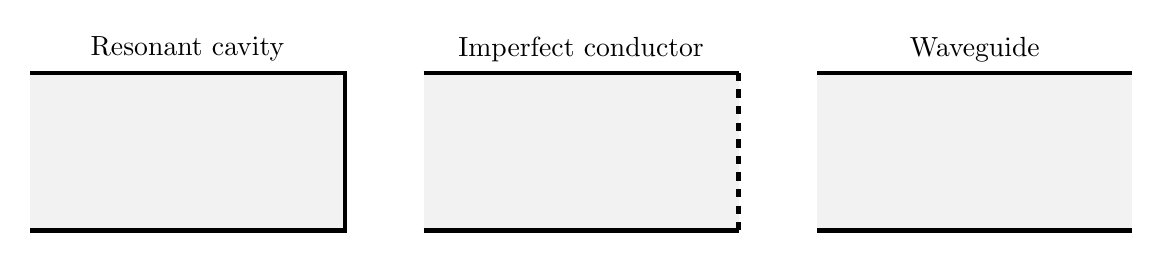
\begin{tikzpicture}
    \node at (2, 2.3) {Resonant cavity};
    \fill[black!5!white] (0, 0) rectangle (4, 2);
    \draw[ultra thick] (0, 0) to (4, 0) to (4, 2) to (0, 2);

    \node at (7, 2.3) {Imperfect conductor};
    \fill[black!5!white] (5, 0) rectangle (9, 2);
    \draw[ultra thick] (5, 0) to (9, 0);
    \draw[ultra thick, dashed] (9, 2) to (9, 0);
    \draw[ultra thick] (5, 2) to (9, 2);

    \node at (12, 2.3) {Waveguide};
    \fill[black!5!white] (10, 0) rectangle (14, 2);
    \draw[ultra thick] (10, 0) to (14, 0);
    \draw[ultra thick] (10, 2) to (14, 2);
\end{tikzpicture}}
    \end{figure}
\end{frame}

\begin{frame}{Rectangular cavity | Symmetry breaking cubby}
    \begin{figure}
        \centering
        \scalebox{0.8}{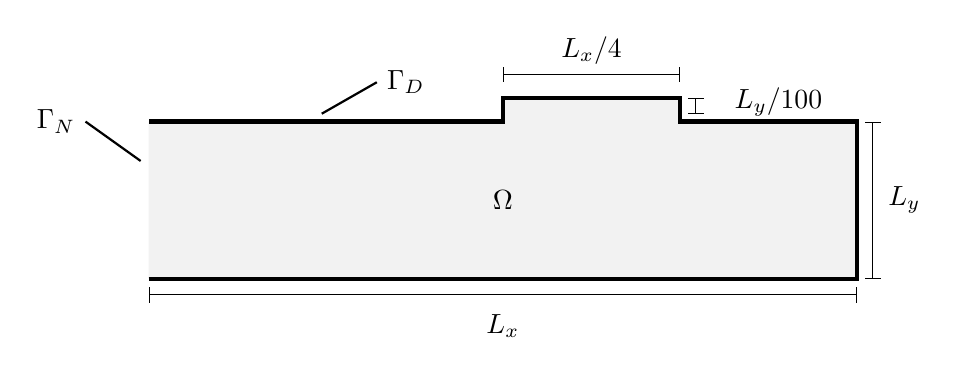
\begin{tikzpicture}
    \fill[black!5!white] (0, 0) to (9, 0) to (9, 2) to (6.75, 2) to (6.75, 2.3) to (4.5, 2.3) to (4.5, 2) to (0, 2);
    \draw[ultra thick] (0, 0) to (9, 0) to (9, 2) to (6.75, 2) to (6.75, 2.3) to (4.5, 2.3) to (4.5, 2) to (0, 2);
    \draw[thick] (-0.8, 2) node[left] {$\Gamma_N$} to (-0.1, 1.5);
    \draw[thick] (2.9, 2.5) node[right] {$\Gamma_D$} to (2.2, 2.1);
    \draw[|-|] (0, -0.2) to (9, -0.2);
    \draw[|-|] (9.2, 0) to (9.2, 2);
    \draw[|-|] (6.75, 2.6) to (4.5, 2.6);
    \draw[|-|] (6.95, 2.1) to (6.95, 2.3);
    \node at (4.5, -0.6) {$L_x$};
    \node at (9.6, 1) {$L_y$};
    \node at (5.626, 2.9) {$L_x / 4$};
    \node at (8, 2.25) {$L_y / 100$};
    \node at (4.5, 1) {$\Omega$};
\end{tikzpicture}
}
    \end{figure}
\end{frame}

\begin{frame}{Rectangular cavity | Symmetry breaking cubby}
    \begin{figure}
        \centering
        \scalebox{0.8}{%% Creator: Matplotlib, PGF backend
%%
%% To include the figure in your LaTeX document, write
%%   \input{<filename>.pgf}
%%
%% Make sure the required packages are loaded in your preamble
%%   \usepackage{pgf}
%%
%% Also ensure that all the required font packages are loaded; for instance,
%% the lmodern package is sometimes necessary when using math font.
%%   \usepackage{lmodern}
%%
%% Figures using additional raster images can only be included by \input if
%% they are in the same directory as the main LaTeX file. For loading figures
%% from other directories you can use the `import` package
%%   \usepackage{import}
%%
%% and then include the figures with
%%   \import{<path to file>}{<filename>.pgf}
%%
%% Matplotlib used the following preamble
%%   \usepackage{fontspec}
%%   \setmainfont{DejaVuSans.ttf}[Path=\detokenize{C:/Users/Fabio/Anaconda3/Lib/site-packages/matplotlib/mpl-data/fonts/ttf/}]
%%   \setsansfont{DejaVuSans.ttf}[Path=\detokenize{C:/Users/Fabio/Anaconda3/Lib/site-packages/matplotlib/mpl-data/fonts/ttf/}]
%%   \setmonofont{DejaVuSansMono.ttf}[Path=\detokenize{C:/Users/Fabio/Anaconda3/Lib/site-packages/matplotlib/mpl-data/fonts/ttf/}]
%%
\begingroup%
\makeatletter%
\begin{pgfpicture}%
\pgfpathrectangle{\pgfpointorigin}{\pgfqpoint{5.314460in}{3.950463in}}%
\pgfusepath{use as bounding box, clip}%
\begin{pgfscope}%
\pgfsetbuttcap%
\pgfsetmiterjoin%
\pgfsetlinewidth{0.000000pt}%
\definecolor{currentstroke}{rgb}{1.000000,1.000000,1.000000}%
\pgfsetstrokecolor{currentstroke}%
\pgfsetstrokeopacity{0.000000}%
\pgfsetdash{}{0pt}%
\pgfpathmoveto{\pgfqpoint{0.000000in}{0.000000in}}%
\pgfpathlineto{\pgfqpoint{5.314460in}{0.000000in}}%
\pgfpathlineto{\pgfqpoint{5.314460in}{3.950463in}}%
\pgfpathlineto{\pgfqpoint{0.000000in}{3.950463in}}%
\pgfpathlineto{\pgfqpoint{0.000000in}{0.000000in}}%
\pgfpathclose%
\pgfusepath{}%
\end{pgfscope}%
\begin{pgfscope}%
\pgfsetbuttcap%
\pgfsetmiterjoin%
\definecolor{currentfill}{rgb}{1.000000,1.000000,1.000000}%
\pgfsetfillcolor{currentfill}%
\pgfsetlinewidth{0.000000pt}%
\definecolor{currentstroke}{rgb}{0.000000,0.000000,0.000000}%
\pgfsetstrokecolor{currentstroke}%
\pgfsetstrokeopacity{0.000000}%
\pgfsetdash{}{0pt}%
\pgfpathmoveto{\pgfqpoint{0.816045in}{0.823031in}}%
\pgfpathlineto{\pgfqpoint{5.117295in}{0.823031in}}%
\pgfpathlineto{\pgfqpoint{5.117295in}{3.568486in}}%
\pgfpathlineto{\pgfqpoint{0.816045in}{3.568486in}}%
\pgfpathlineto{\pgfqpoint{0.816045in}{0.823031in}}%
\pgfpathclose%
\pgfusepath{fill}%
\end{pgfscope}%
\begin{pgfscope}%
\pgfsetbuttcap%
\pgfsetroundjoin%
\definecolor{currentfill}{rgb}{0.000000,0.000000,0.000000}%
\pgfsetfillcolor{currentfill}%
\pgfsetlinewidth{0.803000pt}%
\definecolor{currentstroke}{rgb}{0.000000,0.000000,0.000000}%
\pgfsetstrokecolor{currentstroke}%
\pgfsetdash{}{0pt}%
\pgfsys@defobject{currentmarker}{\pgfqpoint{0.000000in}{-0.048611in}}{\pgfqpoint{0.000000in}{0.000000in}}{%
\pgfpathmoveto{\pgfqpoint{0.000000in}{0.000000in}}%
\pgfpathlineto{\pgfqpoint{0.000000in}{-0.048611in}}%
\pgfusepath{stroke,fill}%
}%
\begin{pgfscope}%
\pgfsys@transformshift{0.816045in}{0.823031in}%
\pgfsys@useobject{currentmarker}{}%
\end{pgfscope}%
\end{pgfscope}%
\begin{pgfscope}%
\pgfsetbuttcap%
\pgfsetroundjoin%
\definecolor{currentfill}{rgb}{0.000000,0.000000,0.000000}%
\pgfsetfillcolor{currentfill}%
\pgfsetlinewidth{0.803000pt}%
\definecolor{currentstroke}{rgb}{0.000000,0.000000,0.000000}%
\pgfsetstrokecolor{currentstroke}%
\pgfsetdash{}{0pt}%
\pgfsys@defobject{currentmarker}{\pgfqpoint{0.000000in}{-0.048611in}}{\pgfqpoint{0.000000in}{0.000000in}}{%
\pgfpathmoveto{\pgfqpoint{0.000000in}{0.000000in}}%
\pgfpathlineto{\pgfqpoint{0.000000in}{-0.048611in}}%
\pgfusepath{stroke,fill}%
}%
\begin{pgfscope}%
\pgfsys@transformshift{1.676295in}{0.823031in}%
\pgfsys@useobject{currentmarker}{}%
\end{pgfscope}%
\end{pgfscope}%
\begin{pgfscope}%
\pgfsetbuttcap%
\pgfsetroundjoin%
\definecolor{currentfill}{rgb}{0.000000,0.000000,0.000000}%
\pgfsetfillcolor{currentfill}%
\pgfsetlinewidth{0.803000pt}%
\definecolor{currentstroke}{rgb}{0.000000,0.000000,0.000000}%
\pgfsetstrokecolor{currentstroke}%
\pgfsetdash{}{0pt}%
\pgfsys@defobject{currentmarker}{\pgfqpoint{0.000000in}{-0.048611in}}{\pgfqpoint{0.000000in}{0.000000in}}{%
\pgfpathmoveto{\pgfqpoint{0.000000in}{0.000000in}}%
\pgfpathlineto{\pgfqpoint{0.000000in}{-0.048611in}}%
\pgfusepath{stroke,fill}%
}%
\begin{pgfscope}%
\pgfsys@transformshift{2.536545in}{0.823031in}%
\pgfsys@useobject{currentmarker}{}%
\end{pgfscope}%
\end{pgfscope}%
\begin{pgfscope}%
\pgfsetbuttcap%
\pgfsetroundjoin%
\definecolor{currentfill}{rgb}{0.000000,0.000000,0.000000}%
\pgfsetfillcolor{currentfill}%
\pgfsetlinewidth{0.803000pt}%
\definecolor{currentstroke}{rgb}{0.000000,0.000000,0.000000}%
\pgfsetstrokecolor{currentstroke}%
\pgfsetdash{}{0pt}%
\pgfsys@defobject{currentmarker}{\pgfqpoint{0.000000in}{-0.048611in}}{\pgfqpoint{0.000000in}{0.000000in}}{%
\pgfpathmoveto{\pgfqpoint{0.000000in}{0.000000in}}%
\pgfpathlineto{\pgfqpoint{0.000000in}{-0.048611in}}%
\pgfusepath{stroke,fill}%
}%
\begin{pgfscope}%
\pgfsys@transformshift{3.396795in}{0.823031in}%
\pgfsys@useobject{currentmarker}{}%
\end{pgfscope}%
\end{pgfscope}%
\begin{pgfscope}%
\pgfsetbuttcap%
\pgfsetroundjoin%
\definecolor{currentfill}{rgb}{0.000000,0.000000,0.000000}%
\pgfsetfillcolor{currentfill}%
\pgfsetlinewidth{0.803000pt}%
\definecolor{currentstroke}{rgb}{0.000000,0.000000,0.000000}%
\pgfsetstrokecolor{currentstroke}%
\pgfsetdash{}{0pt}%
\pgfsys@defobject{currentmarker}{\pgfqpoint{0.000000in}{-0.048611in}}{\pgfqpoint{0.000000in}{0.000000in}}{%
\pgfpathmoveto{\pgfqpoint{0.000000in}{0.000000in}}%
\pgfpathlineto{\pgfqpoint{0.000000in}{-0.048611in}}%
\pgfusepath{stroke,fill}%
}%
\begin{pgfscope}%
\pgfsys@transformshift{4.257045in}{0.823031in}%
\pgfsys@useobject{currentmarker}{}%
\end{pgfscope}%
\end{pgfscope}%
\begin{pgfscope}%
\pgfsetbuttcap%
\pgfsetroundjoin%
\definecolor{currentfill}{rgb}{0.000000,0.000000,0.000000}%
\pgfsetfillcolor{currentfill}%
\pgfsetlinewidth{0.803000pt}%
\definecolor{currentstroke}{rgb}{0.000000,0.000000,0.000000}%
\pgfsetstrokecolor{currentstroke}%
\pgfsetdash{}{0pt}%
\pgfsys@defobject{currentmarker}{\pgfqpoint{0.000000in}{-0.048611in}}{\pgfqpoint{0.000000in}{0.000000in}}{%
\pgfpathmoveto{\pgfqpoint{0.000000in}{0.000000in}}%
\pgfpathlineto{\pgfqpoint{0.000000in}{-0.048611in}}%
\pgfusepath{stroke,fill}%
}%
\begin{pgfscope}%
\pgfsys@transformshift{5.117295in}{0.823031in}%
\pgfsys@useobject{currentmarker}{}%
\end{pgfscope}%
\end{pgfscope}%
\begin{pgfscope}%
\pgfpathrectangle{\pgfqpoint{0.816045in}{0.823031in}}{\pgfqpoint{4.301250in}{2.745455in}}%
\pgfusepath{clip}%
\pgfsetrectcap%
\pgfsetroundjoin%
\pgfsetlinewidth{0.803000pt}%
\definecolor{currentstroke}{rgb}{0.690196,0.690196,0.690196}%
\pgfsetstrokecolor{currentstroke}%
\pgfsetdash{}{0pt}%
\pgfpathmoveto{\pgfqpoint{0.816045in}{1.124514in}}%
\pgfpathlineto{\pgfqpoint{5.117295in}{1.124514in}}%
\pgfusepath{stroke}%
\end{pgfscope}%
\begin{pgfscope}%
\pgfsetbuttcap%
\pgfsetroundjoin%
\definecolor{currentfill}{rgb}{0.000000,0.000000,0.000000}%
\pgfsetfillcolor{currentfill}%
\pgfsetlinewidth{0.803000pt}%
\definecolor{currentstroke}{rgb}{0.000000,0.000000,0.000000}%
\pgfsetstrokecolor{currentstroke}%
\pgfsetdash{}{0pt}%
\pgfsys@defobject{currentmarker}{\pgfqpoint{-0.048611in}{0.000000in}}{\pgfqpoint{-0.000000in}{0.000000in}}{%
\pgfpathmoveto{\pgfqpoint{-0.000000in}{0.000000in}}%
\pgfpathlineto{\pgfqpoint{-0.048611in}{0.000000in}}%
\pgfusepath{stroke,fill}%
}%
\begin{pgfscope}%
\pgfsys@transformshift{0.816045in}{1.124514in}%
\pgfsys@useobject{currentmarker}{}%
\end{pgfscope}%
\end{pgfscope}%
\begin{pgfscope}%
\definecolor{textcolor}{rgb}{0.000000,0.000000,0.000000}%
\pgfsetstrokecolor{textcolor}%
\pgfsetfillcolor{textcolor}%
\pgftext[x=0.408944in, y=1.066477in, left, base]{\color{textcolor}\rmfamily\fontsize{11.000000}{13.200000}\selectfont \(\displaystyle {10^{-8}}\)}%
\end{pgfscope}%
\begin{pgfscope}%
\pgfpathrectangle{\pgfqpoint{0.816045in}{0.823031in}}{\pgfqpoint{4.301250in}{2.745455in}}%
\pgfusepath{clip}%
\pgfsetrectcap%
\pgfsetroundjoin%
\pgfsetlinewidth{0.803000pt}%
\definecolor{currentstroke}{rgb}{0.690196,0.690196,0.690196}%
\pgfsetstrokecolor{currentstroke}%
\pgfsetdash{}{0pt}%
\pgfpathmoveto{\pgfqpoint{0.816045in}{1.546434in}}%
\pgfpathlineto{\pgfqpoint{5.117295in}{1.546434in}}%
\pgfusepath{stroke}%
\end{pgfscope}%
\begin{pgfscope}%
\pgfsetbuttcap%
\pgfsetroundjoin%
\definecolor{currentfill}{rgb}{0.000000,0.000000,0.000000}%
\pgfsetfillcolor{currentfill}%
\pgfsetlinewidth{0.803000pt}%
\definecolor{currentstroke}{rgb}{0.000000,0.000000,0.000000}%
\pgfsetstrokecolor{currentstroke}%
\pgfsetdash{}{0pt}%
\pgfsys@defobject{currentmarker}{\pgfqpoint{-0.048611in}{0.000000in}}{\pgfqpoint{-0.000000in}{0.000000in}}{%
\pgfpathmoveto{\pgfqpoint{-0.000000in}{0.000000in}}%
\pgfpathlineto{\pgfqpoint{-0.048611in}{0.000000in}}%
\pgfusepath{stroke,fill}%
}%
\begin{pgfscope}%
\pgfsys@transformshift{0.816045in}{1.546434in}%
\pgfsys@useobject{currentmarker}{}%
\end{pgfscope}%
\end{pgfscope}%
\begin{pgfscope}%
\definecolor{textcolor}{rgb}{0.000000,0.000000,0.000000}%
\pgfsetstrokecolor{textcolor}%
\pgfsetfillcolor{textcolor}%
\pgftext[x=0.408944in, y=1.488396in, left, base]{\color{textcolor}\rmfamily\fontsize{11.000000}{13.200000}\selectfont \(\displaystyle {10^{-6}}\)}%
\end{pgfscope}%
\begin{pgfscope}%
\pgfpathrectangle{\pgfqpoint{0.816045in}{0.823031in}}{\pgfqpoint{4.301250in}{2.745455in}}%
\pgfusepath{clip}%
\pgfsetrectcap%
\pgfsetroundjoin%
\pgfsetlinewidth{0.803000pt}%
\definecolor{currentstroke}{rgb}{0.690196,0.690196,0.690196}%
\pgfsetstrokecolor{currentstroke}%
\pgfsetdash{}{0pt}%
\pgfpathmoveto{\pgfqpoint{0.816045in}{1.968353in}}%
\pgfpathlineto{\pgfqpoint{5.117295in}{1.968353in}}%
\pgfusepath{stroke}%
\end{pgfscope}%
\begin{pgfscope}%
\pgfsetbuttcap%
\pgfsetroundjoin%
\definecolor{currentfill}{rgb}{0.000000,0.000000,0.000000}%
\pgfsetfillcolor{currentfill}%
\pgfsetlinewidth{0.803000pt}%
\definecolor{currentstroke}{rgb}{0.000000,0.000000,0.000000}%
\pgfsetstrokecolor{currentstroke}%
\pgfsetdash{}{0pt}%
\pgfsys@defobject{currentmarker}{\pgfqpoint{-0.048611in}{0.000000in}}{\pgfqpoint{-0.000000in}{0.000000in}}{%
\pgfpathmoveto{\pgfqpoint{-0.000000in}{0.000000in}}%
\pgfpathlineto{\pgfqpoint{-0.048611in}{0.000000in}}%
\pgfusepath{stroke,fill}%
}%
\begin{pgfscope}%
\pgfsys@transformshift{0.816045in}{1.968353in}%
\pgfsys@useobject{currentmarker}{}%
\end{pgfscope}%
\end{pgfscope}%
\begin{pgfscope}%
\definecolor{textcolor}{rgb}{0.000000,0.000000,0.000000}%
\pgfsetstrokecolor{textcolor}%
\pgfsetfillcolor{textcolor}%
\pgftext[x=0.408944in, y=1.910316in, left, base]{\color{textcolor}\rmfamily\fontsize{11.000000}{13.200000}\selectfont \(\displaystyle {10^{-4}}\)}%
\end{pgfscope}%
\begin{pgfscope}%
\pgfpathrectangle{\pgfqpoint{0.816045in}{0.823031in}}{\pgfqpoint{4.301250in}{2.745455in}}%
\pgfusepath{clip}%
\pgfsetrectcap%
\pgfsetroundjoin%
\pgfsetlinewidth{0.803000pt}%
\definecolor{currentstroke}{rgb}{0.690196,0.690196,0.690196}%
\pgfsetstrokecolor{currentstroke}%
\pgfsetdash{}{0pt}%
\pgfpathmoveto{\pgfqpoint{0.816045in}{2.390273in}}%
\pgfpathlineto{\pgfqpoint{5.117295in}{2.390273in}}%
\pgfusepath{stroke}%
\end{pgfscope}%
\begin{pgfscope}%
\pgfsetbuttcap%
\pgfsetroundjoin%
\definecolor{currentfill}{rgb}{0.000000,0.000000,0.000000}%
\pgfsetfillcolor{currentfill}%
\pgfsetlinewidth{0.803000pt}%
\definecolor{currentstroke}{rgb}{0.000000,0.000000,0.000000}%
\pgfsetstrokecolor{currentstroke}%
\pgfsetdash{}{0pt}%
\pgfsys@defobject{currentmarker}{\pgfqpoint{-0.048611in}{0.000000in}}{\pgfqpoint{-0.000000in}{0.000000in}}{%
\pgfpathmoveto{\pgfqpoint{-0.000000in}{0.000000in}}%
\pgfpathlineto{\pgfqpoint{-0.048611in}{0.000000in}}%
\pgfusepath{stroke,fill}%
}%
\begin{pgfscope}%
\pgfsys@transformshift{0.816045in}{2.390273in}%
\pgfsys@useobject{currentmarker}{}%
\end{pgfscope}%
\end{pgfscope}%
\begin{pgfscope}%
\definecolor{textcolor}{rgb}{0.000000,0.000000,0.000000}%
\pgfsetstrokecolor{textcolor}%
\pgfsetfillcolor{textcolor}%
\pgftext[x=0.408944in, y=2.332235in, left, base]{\color{textcolor}\rmfamily\fontsize{11.000000}{13.200000}\selectfont \(\displaystyle {10^{-2}}\)}%
\end{pgfscope}%
\begin{pgfscope}%
\pgfpathrectangle{\pgfqpoint{0.816045in}{0.823031in}}{\pgfqpoint{4.301250in}{2.745455in}}%
\pgfusepath{clip}%
\pgfsetrectcap%
\pgfsetroundjoin%
\pgfsetlinewidth{0.803000pt}%
\definecolor{currentstroke}{rgb}{0.690196,0.690196,0.690196}%
\pgfsetstrokecolor{currentstroke}%
\pgfsetdash{}{0pt}%
\pgfpathmoveto{\pgfqpoint{0.816045in}{2.812192in}}%
\pgfpathlineto{\pgfqpoint{5.117295in}{2.812192in}}%
\pgfusepath{stroke}%
\end{pgfscope}%
\begin{pgfscope}%
\pgfsetbuttcap%
\pgfsetroundjoin%
\definecolor{currentfill}{rgb}{0.000000,0.000000,0.000000}%
\pgfsetfillcolor{currentfill}%
\pgfsetlinewidth{0.803000pt}%
\definecolor{currentstroke}{rgb}{0.000000,0.000000,0.000000}%
\pgfsetstrokecolor{currentstroke}%
\pgfsetdash{}{0pt}%
\pgfsys@defobject{currentmarker}{\pgfqpoint{-0.048611in}{0.000000in}}{\pgfqpoint{-0.000000in}{0.000000in}}{%
\pgfpathmoveto{\pgfqpoint{-0.000000in}{0.000000in}}%
\pgfpathlineto{\pgfqpoint{-0.048611in}{0.000000in}}%
\pgfusepath{stroke,fill}%
}%
\begin{pgfscope}%
\pgfsys@transformshift{0.816045in}{2.812192in}%
\pgfsys@useobject{currentmarker}{}%
\end{pgfscope}%
\end{pgfscope}%
\begin{pgfscope}%
\definecolor{textcolor}{rgb}{0.000000,0.000000,0.000000}%
\pgfsetstrokecolor{textcolor}%
\pgfsetfillcolor{textcolor}%
\pgftext[x=0.500767in, y=2.754155in, left, base]{\color{textcolor}\rmfamily\fontsize{11.000000}{13.200000}\selectfont \(\displaystyle {10^{0}}\)}%
\end{pgfscope}%
\begin{pgfscope}%
\pgfpathrectangle{\pgfqpoint{0.816045in}{0.823031in}}{\pgfqpoint{4.301250in}{2.745455in}}%
\pgfusepath{clip}%
\pgfsetrectcap%
\pgfsetroundjoin%
\pgfsetlinewidth{0.803000pt}%
\definecolor{currentstroke}{rgb}{0.690196,0.690196,0.690196}%
\pgfsetstrokecolor{currentstroke}%
\pgfsetdash{}{0pt}%
\pgfpathmoveto{\pgfqpoint{0.816045in}{3.234112in}}%
\pgfpathlineto{\pgfqpoint{5.117295in}{3.234112in}}%
\pgfusepath{stroke}%
\end{pgfscope}%
\begin{pgfscope}%
\pgfsetbuttcap%
\pgfsetroundjoin%
\definecolor{currentfill}{rgb}{0.000000,0.000000,0.000000}%
\pgfsetfillcolor{currentfill}%
\pgfsetlinewidth{0.803000pt}%
\definecolor{currentstroke}{rgb}{0.000000,0.000000,0.000000}%
\pgfsetstrokecolor{currentstroke}%
\pgfsetdash{}{0pt}%
\pgfsys@defobject{currentmarker}{\pgfqpoint{-0.048611in}{0.000000in}}{\pgfqpoint{-0.000000in}{0.000000in}}{%
\pgfpathmoveto{\pgfqpoint{-0.000000in}{0.000000in}}%
\pgfpathlineto{\pgfqpoint{-0.048611in}{0.000000in}}%
\pgfusepath{stroke,fill}%
}%
\begin{pgfscope}%
\pgfsys@transformshift{0.816045in}{3.234112in}%
\pgfsys@useobject{currentmarker}{}%
\end{pgfscope}%
\end{pgfscope}%
\begin{pgfscope}%
\definecolor{textcolor}{rgb}{0.000000,0.000000,0.000000}%
\pgfsetstrokecolor{textcolor}%
\pgfsetfillcolor{textcolor}%
\pgftext[x=0.500767in, y=3.176074in, left, base]{\color{textcolor}\rmfamily\fontsize{11.000000}{13.200000}\selectfont \(\displaystyle {10^{2}}\)}%
\end{pgfscope}%
\begin{pgfscope}%
\definecolor{textcolor}{rgb}{0.000000,0.000000,0.000000}%
\pgfsetstrokecolor{textcolor}%
\pgfsetfillcolor{textcolor}%
\pgftext[x=0.353389in,y=2.195759in,,bottom,rotate=90.000000]{\color{textcolor}\rmfamily\fontsize{11.000000}{13.200000}\selectfont \(\displaystyle ||\mathbf{\tilde{u}}_z^{(S)}|_{\Gamma_N}(\omega) - \mathbf{u}|_{\Gamma_N}(\omega)||_{M(\Gamma_N)} / ||\mathbf{\tilde{u}}_z^{(S)}|_{\Gamma_N}(\omega)||_{M(\Gamma_N)}\)}%
\end{pgfscope}%
\begin{pgfscope}%
\pgfpathrectangle{\pgfqpoint{0.816045in}{0.823031in}}{\pgfqpoint{4.301250in}{2.745455in}}%
\pgfusepath{clip}%
\pgfsetrectcap%
\pgfsetroundjoin%
\pgfsetlinewidth{1.505625pt}%
\definecolor{currentstroke}{rgb}{0.001462,0.000466,0.013866}%
\pgfsetstrokecolor{currentstroke}%
\pgfsetdash{}{0pt}%
\pgfpathmoveto{\pgfqpoint{0.813895in}{2.418879in}}%
\pgfpathlineto{\pgfqpoint{0.818200in}{2.421382in}}%
\pgfpathlineto{\pgfqpoint{0.822506in}{2.524354in}}%
\pgfpathlineto{\pgfqpoint{0.831117in}{2.606920in}}%
\pgfpathlineto{\pgfqpoint{0.839728in}{2.653565in}}%
\pgfpathlineto{\pgfqpoint{0.852645in}{2.701917in}}%
\pgfpathlineto{\pgfqpoint{0.869867in}{2.749927in}}%
\pgfpathlineto{\pgfqpoint{0.891395in}{2.799565in}}%
\pgfpathlineto{\pgfqpoint{0.934450in}{2.896812in}}%
\pgfpathlineto{\pgfqpoint{0.947367in}{2.932906in}}%
\pgfpathlineto{\pgfqpoint{0.960283in}{2.979168in}}%
\pgfpathlineto{\pgfqpoint{0.968894in}{3.022411in}}%
\pgfpathlineto{\pgfqpoint{0.973200in}{3.052088in}}%
\pgfpathlineto{\pgfqpoint{0.977506in}{3.093215in}}%
\pgfpathlineto{\pgfqpoint{0.981811in}{3.163152in}}%
\pgfpathlineto{\pgfqpoint{0.986117in}{3.299494in}}%
\pgfpathlineto{\pgfqpoint{0.990422in}{3.148337in}}%
\pgfpathlineto{\pgfqpoint{0.994728in}{3.092540in}}%
\pgfpathlineto{\pgfqpoint{1.003339in}{3.035979in}}%
\pgfpathlineto{\pgfqpoint{1.011950in}{3.003797in}}%
\pgfpathlineto{\pgfqpoint{1.020561in}{2.981793in}}%
\pgfpathlineto{\pgfqpoint{1.033478in}{2.958551in}}%
\pgfpathlineto{\pgfqpoint{1.046394in}{2.941917in}}%
\pgfpathlineto{\pgfqpoint{1.063617in}{2.925627in}}%
\pgfpathlineto{\pgfqpoint{1.080839in}{2.913472in}}%
\pgfpathlineto{\pgfqpoint{1.102367in}{2.901913in}}%
\pgfpathlineto{\pgfqpoint{1.128200in}{2.891459in}}%
\pgfpathlineto{\pgfqpoint{1.162644in}{2.881150in}}%
\pgfpathlineto{\pgfqpoint{1.205700in}{2.871837in}}%
\pgfpathlineto{\pgfqpoint{1.261672in}{2.863244in}}%
\pgfpathlineto{\pgfqpoint{1.334866in}{2.855447in}}%
\pgfpathlineto{\pgfqpoint{1.433894in}{2.848307in}}%
\pgfpathlineto{\pgfqpoint{1.571672in}{2.841751in}}%
\pgfpathlineto{\pgfqpoint{1.774033in}{2.835477in}}%
\pgfpathlineto{\pgfqpoint{2.140004in}{2.827747in}}%
\pgfpathlineto{\pgfqpoint{2.592087in}{2.817538in}}%
\pgfpathlineto{\pgfqpoint{2.794448in}{2.809933in}}%
\pgfpathlineto{\pgfqpoint{2.932226in}{2.801780in}}%
\pgfpathlineto{\pgfqpoint{3.031254in}{2.792955in}}%
\pgfpathlineto{\pgfqpoint{3.104448in}{2.783550in}}%
\pgfpathlineto{\pgfqpoint{3.160420in}{2.773560in}}%
\pgfpathlineto{\pgfqpoint{3.207781in}{2.762001in}}%
\pgfpathlineto{\pgfqpoint{3.242226in}{2.750757in}}%
\pgfpathlineto{\pgfqpoint{3.272364in}{2.737845in}}%
\pgfpathlineto{\pgfqpoint{3.298198in}{2.723222in}}%
\pgfpathlineto{\pgfqpoint{3.319725in}{2.707066in}}%
\pgfpathlineto{\pgfqpoint{3.336948in}{2.689985in}}%
\pgfpathlineto{\pgfqpoint{3.349864in}{2.673321in}}%
\pgfpathlineto{\pgfqpoint{3.362781in}{2.651271in}}%
\pgfpathlineto{\pgfqpoint{3.371392in}{2.631679in}}%
\pgfpathlineto{\pgfqpoint{3.380003in}{2.605275in}}%
\pgfpathlineto{\pgfqpoint{3.388614in}{2.565653in}}%
\pgfpathlineto{\pgfqpoint{3.392920in}{2.535427in}}%
\pgfpathlineto{\pgfqpoint{3.397225in}{2.488467in}}%
\pgfpathlineto{\pgfqpoint{3.401531in}{2.381986in}}%
\pgfpathlineto{\pgfqpoint{3.405837in}{2.402844in}}%
\pgfpathlineto{\pgfqpoint{3.410142in}{2.498632in}}%
\pgfpathlineto{\pgfqpoint{3.418753in}{2.576942in}}%
\pgfpathlineto{\pgfqpoint{3.427364in}{2.620412in}}%
\pgfpathlineto{\pgfqpoint{3.440281in}{2.663952in}}%
\pgfpathlineto{\pgfqpoint{3.453198in}{2.695626in}}%
\pgfpathlineto{\pgfqpoint{3.470420in}{2.728642in}}%
\pgfpathlineto{\pgfqpoint{3.491948in}{2.761896in}}%
\pgfpathlineto{\pgfqpoint{3.517781in}{2.795468in}}%
\pgfpathlineto{\pgfqpoint{3.552225in}{2.834857in}}%
\pgfpathlineto{\pgfqpoint{3.646947in}{2.940360in}}%
\pgfpathlineto{\pgfqpoint{3.672781in}{2.975413in}}%
\pgfpathlineto{\pgfqpoint{3.690003in}{3.003141in}}%
\pgfpathlineto{\pgfqpoint{3.707225in}{3.037173in}}%
\pgfpathlineto{\pgfqpoint{3.720142in}{3.070157in}}%
\pgfpathlineto{\pgfqpoint{3.728753in}{3.098712in}}%
\pgfpathlineto{\pgfqpoint{3.737364in}{3.137429in}}%
\pgfpathlineto{\pgfqpoint{3.741670in}{3.163989in}}%
\pgfpathlineto{\pgfqpoint{3.745975in}{3.200232in}}%
\pgfpathlineto{\pgfqpoint{3.750281in}{3.258665in}}%
\pgfpathlineto{\pgfqpoint{3.754586in}{3.443692in}}%
\pgfpathlineto{\pgfqpoint{3.758892in}{3.289989in}}%
\pgfpathlineto{\pgfqpoint{3.763197in}{3.219687in}}%
\pgfpathlineto{\pgfqpoint{3.771808in}{3.154914in}}%
\pgfpathlineto{\pgfqpoint{3.780419in}{3.119011in}}%
\pgfpathlineto{\pgfqpoint{3.789031in}{3.094477in}}%
\pgfpathlineto{\pgfqpoint{3.801947in}{3.068380in}}%
\pgfpathlineto{\pgfqpoint{3.814864in}{3.049496in}}%
\pgfpathlineto{\pgfqpoint{3.832086in}{3.030784in}}%
\pgfpathlineto{\pgfqpoint{3.849308in}{3.016678in}}%
\pgfpathlineto{\pgfqpoint{3.870836in}{3.003176in}}%
\pgfpathlineto{\pgfqpoint{3.896669in}{2.990967in}}%
\pgfpathlineto{\pgfqpoint{3.926808in}{2.980372in}}%
\pgfpathlineto{\pgfqpoint{3.961253in}{2.971512in}}%
\pgfpathlineto{\pgfqpoint{4.004308in}{2.963776in}}%
\pgfpathlineto{\pgfqpoint{4.055975in}{2.957925in}}%
\pgfpathlineto{\pgfqpoint{4.111947in}{2.954695in}}%
\pgfpathlineto{\pgfqpoint{4.176530in}{2.954211in}}%
\pgfpathlineto{\pgfqpoint{4.241113in}{2.956950in}}%
\pgfpathlineto{\pgfqpoint{4.301391in}{2.962684in}}%
\pgfpathlineto{\pgfqpoint{4.353058in}{2.970661in}}%
\pgfpathlineto{\pgfqpoint{4.396113in}{2.980261in}}%
\pgfpathlineto{\pgfqpoint{4.430558in}{2.990681in}}%
\pgfpathlineto{\pgfqpoint{4.460697in}{3.002682in}}%
\pgfpathlineto{\pgfqpoint{4.486530in}{3.016104in}}%
\pgfpathlineto{\pgfqpoint{4.508058in}{3.030579in}}%
\pgfpathlineto{\pgfqpoint{4.525280in}{3.045383in}}%
\pgfpathlineto{\pgfqpoint{4.542502in}{3.064603in}}%
\pgfpathlineto{\pgfqpoint{4.555419in}{3.083583in}}%
\pgfpathlineto{\pgfqpoint{4.568335in}{3.109182in}}%
\pgfpathlineto{\pgfqpoint{4.576946in}{3.132583in}}%
\pgfpathlineto{\pgfqpoint{4.585558in}{3.165563in}}%
\pgfpathlineto{\pgfqpoint{4.589863in}{3.188656in}}%
\pgfpathlineto{\pgfqpoint{4.594169in}{3.220259in}}%
\pgfpathlineto{\pgfqpoint{4.598474in}{3.269755in}}%
\pgfpathlineto{\pgfqpoint{4.602780in}{3.377288in}}%
\pgfpathlineto{\pgfqpoint{4.607085in}{3.325373in}}%
\pgfpathlineto{\pgfqpoint{4.611391in}{3.246223in}}%
\pgfpathlineto{\pgfqpoint{4.620002in}{3.173214in}}%
\pgfpathlineto{\pgfqpoint{4.628613in}{3.131667in}}%
\pgfpathlineto{\pgfqpoint{4.641530in}{3.090000in}}%
\pgfpathlineto{\pgfqpoint{4.654446in}{3.059911in}}%
\pgfpathlineto{\pgfqpoint{4.671669in}{3.028970in}}%
\pgfpathlineto{\pgfqpoint{4.688891in}{3.004072in}}%
\pgfpathlineto{\pgfqpoint{4.710419in}{2.978042in}}%
\pgfpathlineto{\pgfqpoint{4.736252in}{2.951445in}}%
\pgfpathlineto{\pgfqpoint{4.770696in}{2.920718in}}%
\pgfpathlineto{\pgfqpoint{4.818057in}{2.883282in}}%
\pgfpathlineto{\pgfqpoint{4.964446in}{2.771219in}}%
\pgfpathlineto{\pgfqpoint{4.994585in}{2.743249in}}%
\pgfpathlineto{\pgfqpoint{5.020418in}{2.715321in}}%
\pgfpathlineto{\pgfqpoint{5.041946in}{2.687355in}}%
\pgfpathlineto{\pgfqpoint{5.059168in}{2.659795in}}%
\pgfpathlineto{\pgfqpoint{5.072085in}{2.634023in}}%
\pgfpathlineto{\pgfqpoint{5.085001in}{2.600523in}}%
\pgfpathlineto{\pgfqpoint{5.093613in}{2.570365in}}%
\pgfpathlineto{\pgfqpoint{5.102224in}{2.527245in}}%
\pgfpathlineto{\pgfqpoint{5.106529in}{2.495577in}}%
\pgfpathlineto{\pgfqpoint{5.110835in}{2.447949in}}%
\pgfpathlineto{\pgfqpoint{5.115140in}{2.346524in}}%
\pgfpathlineto{\pgfqpoint{5.119446in}{2.345516in}}%
\pgfpathlineto{\pgfqpoint{5.119446in}{2.345516in}}%
\pgfusepath{stroke}%
\end{pgfscope}%
\begin{pgfscope}%
\pgfpathrectangle{\pgfqpoint{0.816045in}{0.823031in}}{\pgfqpoint{4.301250in}{2.745455in}}%
\pgfusepath{clip}%
\pgfsetrectcap%
\pgfsetroundjoin%
\pgfsetlinewidth{1.505625pt}%
\definecolor{currentstroke}{rgb}{0.155850,0.044559,0.325338}%
\pgfsetstrokecolor{currentstroke}%
\pgfsetdash{}{0pt}%
\pgfpathmoveto{\pgfqpoint{0.813895in}{2.420633in}}%
\pgfpathlineto{\pgfqpoint{0.818200in}{2.423139in}}%
\pgfpathlineto{\pgfqpoint{0.822506in}{2.526114in}}%
\pgfpathlineto{\pgfqpoint{0.831117in}{2.608685in}}%
\pgfpathlineto{\pgfqpoint{0.839728in}{2.655336in}}%
\pgfpathlineto{\pgfqpoint{0.852645in}{2.703696in}}%
\pgfpathlineto{\pgfqpoint{0.869867in}{2.751716in}}%
\pgfpathlineto{\pgfqpoint{0.891395in}{2.801366in}}%
\pgfpathlineto{\pgfqpoint{0.934450in}{2.898636in}}%
\pgfpathlineto{\pgfqpoint{0.947367in}{2.934737in}}%
\pgfpathlineto{\pgfqpoint{0.960283in}{2.981005in}}%
\pgfpathlineto{\pgfqpoint{0.968894in}{3.024253in}}%
\pgfpathlineto{\pgfqpoint{0.973200in}{3.053932in}}%
\pgfpathlineto{\pgfqpoint{0.977506in}{3.095061in}}%
\pgfpathlineto{\pgfqpoint{0.981811in}{3.165000in}}%
\pgfpathlineto{\pgfqpoint{0.986117in}{3.301344in}}%
\pgfpathlineto{\pgfqpoint{0.990422in}{3.150189in}}%
\pgfpathlineto{\pgfqpoint{0.994728in}{3.094395in}}%
\pgfpathlineto{\pgfqpoint{1.003339in}{3.037837in}}%
\pgfpathlineto{\pgfqpoint{1.011950in}{3.005659in}}%
\pgfpathlineto{\pgfqpoint{1.020561in}{2.983658in}}%
\pgfpathlineto{\pgfqpoint{1.033478in}{2.960422in}}%
\pgfpathlineto{\pgfqpoint{1.046394in}{2.943794in}}%
\pgfpathlineto{\pgfqpoint{1.063617in}{2.927510in}}%
\pgfpathlineto{\pgfqpoint{1.080839in}{2.915362in}}%
\pgfpathlineto{\pgfqpoint{1.102367in}{2.903810in}}%
\pgfpathlineto{\pgfqpoint{1.128200in}{2.893364in}}%
\pgfpathlineto{\pgfqpoint{1.162644in}{2.883065in}}%
\pgfpathlineto{\pgfqpoint{1.205700in}{2.873761in}}%
\pgfpathlineto{\pgfqpoint{1.261672in}{2.865177in}}%
\pgfpathlineto{\pgfqpoint{1.334866in}{2.857385in}}%
\pgfpathlineto{\pgfqpoint{1.433894in}{2.850238in}}%
\pgfpathlineto{\pgfqpoint{1.571672in}{2.843641in}}%
\pgfpathlineto{\pgfqpoint{1.778338in}{2.837121in}}%
\pgfpathlineto{\pgfqpoint{2.191671in}{2.827879in}}%
\pgfpathlineto{\pgfqpoint{2.587782in}{2.817831in}}%
\pgfpathlineto{\pgfqpoint{2.811670in}{2.809211in}}%
\pgfpathlineto{\pgfqpoint{2.979587in}{2.799797in}}%
\pgfpathlineto{\pgfqpoint{3.113059in}{2.789269in}}%
\pgfpathlineto{\pgfqpoint{3.220698in}{2.777699in}}%
\pgfpathlineto{\pgfqpoint{3.306809in}{2.765485in}}%
\pgfpathlineto{\pgfqpoint{3.380003in}{2.752105in}}%
\pgfpathlineto{\pgfqpoint{3.440281in}{2.738147in}}%
\pgfpathlineto{\pgfqpoint{3.491948in}{2.723203in}}%
\pgfpathlineto{\pgfqpoint{3.535003in}{2.707800in}}%
\pgfpathlineto{\pgfqpoint{3.573753in}{2.690693in}}%
\pgfpathlineto{\pgfqpoint{3.603892in}{2.674374in}}%
\pgfpathlineto{\pgfqpoint{3.629725in}{2.657389in}}%
\pgfpathlineto{\pgfqpoint{3.651253in}{2.640226in}}%
\pgfpathlineto{\pgfqpoint{3.672781in}{2.619036in}}%
\pgfpathlineto{\pgfqpoint{3.690003in}{2.597681in}}%
\pgfpathlineto{\pgfqpoint{3.702920in}{2.577668in}}%
\pgfpathlineto{\pgfqpoint{3.715836in}{2.552164in}}%
\pgfpathlineto{\pgfqpoint{3.724447in}{2.530234in}}%
\pgfpathlineto{\pgfqpoint{3.733058in}{2.501518in}}%
\pgfpathlineto{\pgfqpoint{3.741670in}{2.459781in}}%
\pgfpathlineto{\pgfqpoint{3.745975in}{2.428781in}}%
\pgfpathlineto{\pgfqpoint{3.750281in}{2.381801in}}%
\pgfpathlineto{\pgfqpoint{3.754586in}{2.280980in}}%
\pgfpathlineto{\pgfqpoint{3.758892in}{2.280715in}}%
\pgfpathlineto{\pgfqpoint{3.763197in}{2.381185in}}%
\pgfpathlineto{\pgfqpoint{3.771808in}{2.458385in}}%
\pgfpathlineto{\pgfqpoint{3.780419in}{2.499330in}}%
\pgfpathlineto{\pgfqpoint{3.789031in}{2.527245in}}%
\pgfpathlineto{\pgfqpoint{3.801947in}{2.557255in}}%
\pgfpathlineto{\pgfqpoint{3.814864in}{2.579381in}}%
\pgfpathlineto{\pgfqpoint{3.832086in}{2.601821in}}%
\pgfpathlineto{\pgfqpoint{3.849308in}{2.619180in}}%
\pgfpathlineto{\pgfqpoint{3.870836in}{2.636210in}}%
\pgfpathlineto{\pgfqpoint{3.896669in}{2.651954in}}%
\pgfpathlineto{\pgfqpoint{3.922503in}{2.664032in}}%
\pgfpathlineto{\pgfqpoint{3.952642in}{2.674619in}}%
\pgfpathlineto{\pgfqpoint{3.982780in}{2.682139in}}%
\pgfpathlineto{\pgfqpoint{4.017225in}{2.687472in}}%
\pgfpathlineto{\pgfqpoint{4.051669in}{2.689518in}}%
\pgfpathlineto{\pgfqpoint{4.086114in}{2.688152in}}%
\pgfpathlineto{\pgfqpoint{4.116252in}{2.683767in}}%
\pgfpathlineto{\pgfqpoint{4.142086in}{2.677085in}}%
\pgfpathlineto{\pgfqpoint{4.163614in}{2.668849in}}%
\pgfpathlineto{\pgfqpoint{4.185141in}{2.657314in}}%
\pgfpathlineto{\pgfqpoint{4.202363in}{2.644736in}}%
\pgfpathlineto{\pgfqpoint{4.219586in}{2.627686in}}%
\pgfpathlineto{\pgfqpoint{4.232502in}{2.610362in}}%
\pgfpathlineto{\pgfqpoint{4.245419in}{2.586559in}}%
\pgfpathlineto{\pgfqpoint{4.254030in}{2.564570in}}%
\pgfpathlineto{\pgfqpoint{4.262641in}{2.533468in}}%
\pgfpathlineto{\pgfqpoint{4.271252in}{2.482210in}}%
\pgfpathlineto{\pgfqpoint{4.275558in}{2.436714in}}%
\pgfpathlineto{\pgfqpoint{4.279863in}{2.337397in}}%
\pgfpathlineto{\pgfqpoint{4.284169in}{2.338587in}}%
\pgfpathlineto{\pgfqpoint{4.288475in}{2.440583in}}%
\pgfpathlineto{\pgfqpoint{4.297086in}{2.520846in}}%
\pgfpathlineto{\pgfqpoint{4.305697in}{2.564902in}}%
\pgfpathlineto{\pgfqpoint{4.318613in}{2.608802in}}%
\pgfpathlineto{\pgfqpoint{4.331530in}{2.640588in}}%
\pgfpathlineto{\pgfqpoint{4.348752in}{2.673543in}}%
\pgfpathlineto{\pgfqpoint{4.370280in}{2.706495in}}%
\pgfpathlineto{\pgfqpoint{4.396113in}{2.739483in}}%
\pgfpathlineto{\pgfqpoint{4.430558in}{2.777941in}}%
\pgfpathlineto{\pgfqpoint{4.503752in}{2.857682in}}%
\pgfpathlineto{\pgfqpoint{4.525280in}{2.885615in}}%
\pgfpathlineto{\pgfqpoint{4.542502in}{2.912130in}}%
\pgfpathlineto{\pgfqpoint{4.555419in}{2.936248in}}%
\pgfpathlineto{\pgfqpoint{4.568335in}{2.966724in}}%
\pgfpathlineto{\pgfqpoint{4.576946in}{2.993243in}}%
\pgfpathlineto{\pgfqpoint{4.585558in}{3.029239in}}%
\pgfpathlineto{\pgfqpoint{4.594169in}{3.086856in}}%
\pgfpathlineto{\pgfqpoint{4.598474in}{3.137777in}}%
\pgfpathlineto{\pgfqpoint{4.602780in}{3.246713in}}%
\pgfpathlineto{\pgfqpoint{4.607085in}{3.196179in}}%
\pgfpathlineto{\pgfqpoint{4.611391in}{3.118390in}}%
\pgfpathlineto{\pgfqpoint{4.620002in}{3.048039in}}%
\pgfpathlineto{\pgfqpoint{4.628613in}{3.009071in}}%
\pgfpathlineto{\pgfqpoint{4.637224in}{2.982070in}}%
\pgfpathlineto{\pgfqpoint{4.650141in}{2.952609in}}%
\pgfpathlineto{\pgfqpoint{4.663057in}{2.930459in}}%
\pgfpathlineto{\pgfqpoint{4.680280in}{2.907340in}}%
\pgfpathlineto{\pgfqpoint{4.701807in}{2.884489in}}%
\pgfpathlineto{\pgfqpoint{4.727641in}{2.862207in}}%
\pgfpathlineto{\pgfqpoint{4.762085in}{2.837377in}}%
\pgfpathlineto{\pgfqpoint{4.809446in}{2.807758in}}%
\pgfpathlineto{\pgfqpoint{4.938613in}{2.729248in}}%
\pgfpathlineto{\pgfqpoint{4.973057in}{2.704074in}}%
\pgfpathlineto{\pgfqpoint{5.003196in}{2.678167in}}%
\pgfpathlineto{\pgfqpoint{5.024724in}{2.656049in}}%
\pgfpathlineto{\pgfqpoint{5.041946in}{2.634927in}}%
\pgfpathlineto{\pgfqpoint{5.059168in}{2.608973in}}%
\pgfpathlineto{\pgfqpoint{5.072085in}{2.584367in}}%
\pgfpathlineto{\pgfqpoint{5.085001in}{2.552000in}}%
\pgfpathlineto{\pgfqpoint{5.093613in}{2.522580in}}%
\pgfpathlineto{\pgfqpoint{5.102224in}{2.480185in}}%
\pgfpathlineto{\pgfqpoint{5.106529in}{2.448874in}}%
\pgfpathlineto{\pgfqpoint{5.110835in}{2.401600in}}%
\pgfpathlineto{\pgfqpoint{5.115140in}{2.300526in}}%
\pgfpathlineto{\pgfqpoint{5.119446in}{2.299865in}}%
\pgfpathlineto{\pgfqpoint{5.119446in}{2.299865in}}%
\pgfusepath{stroke}%
\end{pgfscope}%
\begin{pgfscope}%
\pgfpathrectangle{\pgfqpoint{0.816045in}{0.823031in}}{\pgfqpoint{4.301250in}{2.745455in}}%
\pgfusepath{clip}%
\pgfsetrectcap%
\pgfsetroundjoin%
\pgfsetlinewidth{1.505625pt}%
\definecolor{currentstroke}{rgb}{0.397674,0.083257,0.433183}%
\pgfsetstrokecolor{currentstroke}%
\pgfsetdash{}{0pt}%
\pgfpathmoveto{\pgfqpoint{0.813895in}{2.262946in}}%
\pgfpathlineto{\pgfqpoint{0.818200in}{2.264931in}}%
\pgfpathlineto{\pgfqpoint{0.822506in}{2.367384in}}%
\pgfpathlineto{\pgfqpoint{0.831117in}{2.448910in}}%
\pgfpathlineto{\pgfqpoint{0.839728in}{2.494512in}}%
\pgfpathlineto{\pgfqpoint{0.852645in}{2.541293in}}%
\pgfpathlineto{\pgfqpoint{0.869867in}{2.587198in}}%
\pgfpathlineto{\pgfqpoint{0.891395in}{2.634186in}}%
\pgfpathlineto{\pgfqpoint{0.930145in}{2.715825in}}%
\pgfpathlineto{\pgfqpoint{0.947367in}{2.760534in}}%
\pgfpathlineto{\pgfqpoint{0.960283in}{2.805161in}}%
\pgfpathlineto{\pgfqpoint{0.968894in}{2.847310in}}%
\pgfpathlineto{\pgfqpoint{0.973200in}{2.876437in}}%
\pgfpathlineto{\pgfqpoint{0.977506in}{2.917014in}}%
\pgfpathlineto{\pgfqpoint{0.981811in}{2.986400in}}%
\pgfpathlineto{\pgfqpoint{0.986117in}{3.122190in}}%
\pgfpathlineto{\pgfqpoint{0.990422in}{2.970481in}}%
\pgfpathlineto{\pgfqpoint{0.994728in}{2.914130in}}%
\pgfpathlineto{\pgfqpoint{1.003339in}{2.856458in}}%
\pgfpathlineto{\pgfqpoint{1.011950in}{2.823161in}}%
\pgfpathlineto{\pgfqpoint{1.020561in}{2.800038in}}%
\pgfpathlineto{\pgfqpoint{1.033478in}{2.775111in}}%
\pgfpathlineto{\pgfqpoint{1.046394in}{2.756781in}}%
\pgfpathlineto{\pgfqpoint{1.063617in}{2.738213in}}%
\pgfpathlineto{\pgfqpoint{1.085144in}{2.720605in}}%
\pgfpathlineto{\pgfqpoint{1.110978in}{2.704322in}}%
\pgfpathlineto{\pgfqpoint{1.141117in}{2.689313in}}%
\pgfpathlineto{\pgfqpoint{1.179867in}{2.673771in}}%
\pgfpathlineto{\pgfqpoint{1.231533in}{2.656852in}}%
\pgfpathlineto{\pgfqpoint{1.300422in}{2.637960in}}%
\pgfpathlineto{\pgfqpoint{1.399450in}{2.614300in}}%
\pgfpathlineto{\pgfqpoint{1.804171in}{2.520720in}}%
\pgfpathlineto{\pgfqpoint{1.903199in}{2.493149in}}%
\pgfpathlineto{\pgfqpoint{1.980699in}{2.468543in}}%
\pgfpathlineto{\pgfqpoint{2.045282in}{2.445023in}}%
\pgfpathlineto{\pgfqpoint{2.101254in}{2.421403in}}%
\pgfpathlineto{\pgfqpoint{2.148616in}{2.397973in}}%
\pgfpathlineto{\pgfqpoint{2.187366in}{2.375332in}}%
\pgfpathlineto{\pgfqpoint{2.217504in}{2.354541in}}%
\pgfpathlineto{\pgfqpoint{2.243338in}{2.333460in}}%
\pgfpathlineto{\pgfqpoint{2.264865in}{2.312511in}}%
\pgfpathlineto{\pgfqpoint{2.286393in}{2.286856in}}%
\pgfpathlineto{\pgfqpoint{2.303615in}{2.260921in}}%
\pgfpathlineto{\pgfqpoint{2.316532in}{2.236242in}}%
\pgfpathlineto{\pgfqpoint{2.329449in}{2.203728in}}%
\pgfpathlineto{\pgfqpoint{2.338060in}{2.174167in}}%
\pgfpathlineto{\pgfqpoint{2.346671in}{2.131594in}}%
\pgfpathlineto{\pgfqpoint{2.350976in}{2.100178in}}%
\pgfpathlineto{\pgfqpoint{2.355282in}{2.052781in}}%
\pgfpathlineto{\pgfqpoint{2.359588in}{1.951514in}}%
\pgfpathlineto{\pgfqpoint{2.363893in}{1.950963in}}%
\pgfpathlineto{\pgfqpoint{2.368199in}{2.050993in}}%
\pgfpathlineto{\pgfqpoint{2.376810in}{2.127386in}}%
\pgfpathlineto{\pgfqpoint{2.385421in}{2.167542in}}%
\pgfpathlineto{\pgfqpoint{2.394032in}{2.194681in}}%
\pgfpathlineto{\pgfqpoint{2.406949in}{2.223542in}}%
\pgfpathlineto{\pgfqpoint{2.419865in}{2.244536in}}%
\pgfpathlineto{\pgfqpoint{2.437087in}{2.265486in}}%
\pgfpathlineto{\pgfqpoint{2.454310in}{2.281365in}}%
\pgfpathlineto{\pgfqpoint{2.475837in}{2.296527in}}%
\pgfpathlineto{\pgfqpoint{2.497365in}{2.307994in}}%
\pgfpathlineto{\pgfqpoint{2.523198in}{2.318061in}}%
\pgfpathlineto{\pgfqpoint{2.549032in}{2.324717in}}%
\pgfpathlineto{\pgfqpoint{2.574865in}{2.328008in}}%
\pgfpathlineto{\pgfqpoint{2.596393in}{2.327706in}}%
\pgfpathlineto{\pgfqpoint{2.613615in}{2.324721in}}%
\pgfpathlineto{\pgfqpoint{2.626532in}{2.320126in}}%
\pgfpathlineto{\pgfqpoint{2.639448in}{2.312397in}}%
\pgfpathlineto{\pgfqpoint{2.648059in}{2.304534in}}%
\pgfpathlineto{\pgfqpoint{2.656671in}{2.293163in}}%
\pgfpathlineto{\pgfqpoint{2.665282in}{2.275835in}}%
\pgfpathlineto{\pgfqpoint{2.673893in}{2.246524in}}%
\pgfpathlineto{\pgfqpoint{2.678198in}{2.222211in}}%
\pgfpathlineto{\pgfqpoint{2.682504in}{2.182292in}}%
\pgfpathlineto{\pgfqpoint{2.686809in}{2.088941in}}%
\pgfpathlineto{\pgfqpoint{2.691115in}{2.096770in}}%
\pgfpathlineto{\pgfqpoint{2.695421in}{2.205802in}}%
\pgfpathlineto{\pgfqpoint{2.704032in}{2.302425in}}%
\pgfpathlineto{\pgfqpoint{2.716948in}{2.396255in}}%
\pgfpathlineto{\pgfqpoint{2.729865in}{2.490858in}}%
\pgfpathlineto{\pgfqpoint{2.734171in}{2.532647in}}%
\pgfpathlineto{\pgfqpoint{2.738476in}{2.591308in}}%
\pgfpathlineto{\pgfqpoint{2.742782in}{2.716820in}}%
\pgfpathlineto{\pgfqpoint{2.747087in}{2.681281in}}%
\pgfpathlineto{\pgfqpoint{2.751393in}{2.599893in}}%
\pgfpathlineto{\pgfqpoint{2.755698in}{2.562325in}}%
\pgfpathlineto{\pgfqpoint{2.764309in}{2.522301in}}%
\pgfpathlineto{\pgfqpoint{2.772920in}{2.500078in}}%
\pgfpathlineto{\pgfqpoint{2.781532in}{2.485619in}}%
\pgfpathlineto{\pgfqpoint{2.794448in}{2.471321in}}%
\pgfpathlineto{\pgfqpoint{2.807365in}{2.461864in}}%
\pgfpathlineto{\pgfqpoint{2.824587in}{2.453339in}}%
\pgfpathlineto{\pgfqpoint{2.846115in}{2.446309in}}%
\pgfpathlineto{\pgfqpoint{2.876254in}{2.439978in}}%
\pgfpathlineto{\pgfqpoint{2.923615in}{2.433808in}}%
\pgfpathlineto{\pgfqpoint{3.014031in}{2.426029in}}%
\pgfpathlineto{\pgfqpoint{3.160420in}{2.412966in}}%
\pgfpathlineto{\pgfqpoint{3.255142in}{2.401246in}}%
\pgfpathlineto{\pgfqpoint{3.332642in}{2.388657in}}%
\pgfpathlineto{\pgfqpoint{3.401531in}{2.374369in}}%
\pgfpathlineto{\pgfqpoint{3.457503in}{2.359842in}}%
\pgfpathlineto{\pgfqpoint{3.509170in}{2.343219in}}%
\pgfpathlineto{\pgfqpoint{3.552225in}{2.326054in}}%
\pgfpathlineto{\pgfqpoint{3.586670in}{2.309231in}}%
\pgfpathlineto{\pgfqpoint{3.616809in}{2.291269in}}%
\pgfpathlineto{\pgfqpoint{3.642642in}{2.272369in}}%
\pgfpathlineto{\pgfqpoint{3.664170in}{2.252950in}}%
\pgfpathlineto{\pgfqpoint{3.681392in}{2.233816in}}%
\pgfpathlineto{\pgfqpoint{3.698614in}{2.209706in}}%
\pgfpathlineto{\pgfqpoint{3.711531in}{2.186388in}}%
\pgfpathlineto{\pgfqpoint{3.724447in}{2.155230in}}%
\pgfpathlineto{\pgfqpoint{3.733058in}{2.126573in}}%
\pgfpathlineto{\pgfqpoint{3.741670in}{2.084904in}}%
\pgfpathlineto{\pgfqpoint{3.745975in}{2.053942in}}%
\pgfpathlineto{\pgfqpoint{3.750281in}{2.007004in}}%
\pgfpathlineto{\pgfqpoint{3.754586in}{1.906226in}}%
\pgfpathlineto{\pgfqpoint{3.758892in}{1.906008in}}%
\pgfpathlineto{\pgfqpoint{3.763197in}{2.006528in}}%
\pgfpathlineto{\pgfqpoint{3.771808in}{2.083835in}}%
\pgfpathlineto{\pgfqpoint{3.780419in}{2.124899in}}%
\pgfpathlineto{\pgfqpoint{3.789031in}{2.152946in}}%
\pgfpathlineto{\pgfqpoint{3.801947in}{2.183177in}}%
\pgfpathlineto{\pgfqpoint{3.814864in}{2.205554in}}%
\pgfpathlineto{\pgfqpoint{3.832086in}{2.228379in}}%
\pgfpathlineto{\pgfqpoint{3.849308in}{2.246180in}}%
\pgfpathlineto{\pgfqpoint{3.870836in}{2.263851in}}%
\pgfpathlineto{\pgfqpoint{3.896669in}{2.280498in}}%
\pgfpathlineto{\pgfqpoint{3.922503in}{2.293637in}}%
\pgfpathlineto{\pgfqpoint{3.952642in}{2.305671in}}%
\pgfpathlineto{\pgfqpoint{3.987086in}{2.315988in}}%
\pgfpathlineto{\pgfqpoint{4.021530in}{2.323182in}}%
\pgfpathlineto{\pgfqpoint{4.055975in}{2.327434in}}%
\pgfpathlineto{\pgfqpoint{4.090419in}{2.328589in}}%
\pgfpathlineto{\pgfqpoint{4.120558in}{2.326624in}}%
\pgfpathlineto{\pgfqpoint{4.146391in}{2.322125in}}%
\pgfpathlineto{\pgfqpoint{4.167919in}{2.315722in}}%
\pgfpathlineto{\pgfqpoint{4.189447in}{2.305930in}}%
\pgfpathlineto{\pgfqpoint{4.206669in}{2.294545in}}%
\pgfpathlineto{\pgfqpoint{4.219586in}{2.282927in}}%
\pgfpathlineto{\pgfqpoint{4.232502in}{2.267318in}}%
\pgfpathlineto{\pgfqpoint{4.245419in}{2.245280in}}%
\pgfpathlineto{\pgfqpoint{4.254030in}{2.224493in}}%
\pgfpathlineto{\pgfqpoint{4.262641in}{2.194616in}}%
\pgfpathlineto{\pgfqpoint{4.266947in}{2.173507in}}%
\pgfpathlineto{\pgfqpoint{4.271252in}{2.144604in}}%
\pgfpathlineto{\pgfqpoint{4.275558in}{2.099738in}}%
\pgfpathlineto{\pgfqpoint{4.279863in}{2.001057in}}%
\pgfpathlineto{\pgfqpoint{4.284169in}{2.002888in}}%
\pgfpathlineto{\pgfqpoint{4.288475in}{2.105531in}}%
\pgfpathlineto{\pgfqpoint{4.297086in}{2.187101in}}%
\pgfpathlineto{\pgfqpoint{4.305697in}{2.232486in}}%
\pgfpathlineto{\pgfqpoint{4.318613in}{2.278416in}}%
\pgfpathlineto{\pgfqpoint{4.331530in}{2.312275in}}%
\pgfpathlineto{\pgfqpoint{4.348752in}{2.348063in}}%
\pgfpathlineto{\pgfqpoint{4.370280in}{2.384662in}}%
\pgfpathlineto{\pgfqpoint{4.396113in}{2.422175in}}%
\pgfpathlineto{\pgfqpoint{4.434863in}{2.472292in}}%
\pgfpathlineto{\pgfqpoint{4.499447in}{2.554805in}}%
\pgfpathlineto{\pgfqpoint{4.525280in}{2.593101in}}%
\pgfpathlineto{\pgfqpoint{4.542502in}{2.623165in}}%
\pgfpathlineto{\pgfqpoint{4.559724in}{2.660144in}}%
\pgfpathlineto{\pgfqpoint{4.572641in}{2.696502in}}%
\pgfpathlineto{\pgfqpoint{4.581252in}{2.728819in}}%
\pgfpathlineto{\pgfqpoint{4.589863in}{2.774846in}}%
\pgfpathlineto{\pgfqpoint{4.594169in}{2.808825in}}%
\pgfpathlineto{\pgfqpoint{4.598474in}{2.860676in}}%
\pgfpathlineto{\pgfqpoint{4.602780in}{2.970544in}}%
\pgfpathlineto{\pgfqpoint{4.607085in}{2.920946in}}%
\pgfpathlineto{\pgfqpoint{4.611391in}{2.844095in}}%
\pgfpathlineto{\pgfqpoint{4.620002in}{2.775629in}}%
\pgfpathlineto{\pgfqpoint{4.628613in}{2.738556in}}%
\pgfpathlineto{\pgfqpoint{4.637224in}{2.713460in}}%
\pgfpathlineto{\pgfqpoint{4.650141in}{2.686875in}}%
\pgfpathlineto{\pgfqpoint{4.663057in}{2.667623in}}%
\pgfpathlineto{\pgfqpoint{4.680280in}{2.648403in}}%
\pgfpathlineto{\pgfqpoint{4.697502in}{2.633671in}}%
\pgfpathlineto{\pgfqpoint{4.719030in}{2.619148in}}%
\pgfpathlineto{\pgfqpoint{4.744863in}{2.605288in}}%
\pgfpathlineto{\pgfqpoint{4.779307in}{2.590373in}}%
\pgfpathlineto{\pgfqpoint{4.830974in}{2.571738in}}%
\pgfpathlineto{\pgfqpoint{4.925696in}{2.538216in}}%
\pgfpathlineto{\pgfqpoint{4.964446in}{2.521022in}}%
\pgfpathlineto{\pgfqpoint{4.994585in}{2.504243in}}%
\pgfpathlineto{\pgfqpoint{5.016113in}{2.489244in}}%
\pgfpathlineto{\pgfqpoint{5.037640in}{2.470217in}}%
\pgfpathlineto{\pgfqpoint{5.054863in}{2.450356in}}%
\pgfpathlineto{\pgfqpoint{5.067779in}{2.431045in}}%
\pgfpathlineto{\pgfqpoint{5.080696in}{2.405345in}}%
\pgfpathlineto{\pgfqpoint{5.089307in}{2.382133in}}%
\pgfpathlineto{\pgfqpoint{5.097918in}{2.349840in}}%
\pgfpathlineto{\pgfqpoint{5.106529in}{2.297419in}}%
\pgfpathlineto{\pgfqpoint{5.110835in}{2.251352in}}%
\pgfpathlineto{\pgfqpoint{5.115140in}{2.151488in}}%
\pgfpathlineto{\pgfqpoint{5.119446in}{2.152041in}}%
\pgfpathlineto{\pgfqpoint{5.119446in}{2.152041in}}%
\pgfusepath{stroke}%
\end{pgfscope}%
\begin{pgfscope}%
\pgfpathrectangle{\pgfqpoint{0.816045in}{0.823031in}}{\pgfqpoint{4.301250in}{2.745455in}}%
\pgfusepath{clip}%
\pgfsetrectcap%
\pgfsetroundjoin%
\pgfsetlinewidth{1.505625pt}%
\definecolor{currentstroke}{rgb}{0.621685,0.164184,0.388781}%
\pgfsetstrokecolor{currentstroke}%
\pgfsetdash{}{0pt}%
\pgfpathmoveto{\pgfqpoint{0.813895in}{1.887700in}}%
\pgfpathlineto{\pgfqpoint{0.818200in}{1.888232in}}%
\pgfpathlineto{\pgfqpoint{0.822506in}{1.989222in}}%
\pgfpathlineto{\pgfqpoint{0.831117in}{2.067784in}}%
\pgfpathlineto{\pgfqpoint{0.839728in}{2.110372in}}%
\pgfpathlineto{\pgfqpoint{0.852645in}{2.152535in}}%
\pgfpathlineto{\pgfqpoint{0.865561in}{2.183244in}}%
\pgfpathlineto{\pgfqpoint{0.882783in}{2.216089in}}%
\pgfpathlineto{\pgfqpoint{0.943061in}{2.322967in}}%
\pgfpathlineto{\pgfqpoint{0.955978in}{2.357278in}}%
\pgfpathlineto{\pgfqpoint{0.964589in}{2.388876in}}%
\pgfpathlineto{\pgfqpoint{0.973200in}{2.436719in}}%
\pgfpathlineto{\pgfqpoint{0.977506in}{2.475113in}}%
\pgfpathlineto{\pgfqpoint{0.981811in}{2.542281in}}%
\pgfpathlineto{\pgfqpoint{0.986117in}{2.675817in}}%
\pgfpathlineto{\pgfqpoint{0.990422in}{2.521816in}}%
\pgfpathlineto{\pgfqpoint{0.994728in}{2.463135in}}%
\pgfpathlineto{\pgfqpoint{1.003339in}{2.400678in}}%
\pgfpathlineto{\pgfqpoint{1.011950in}{2.362419in}}%
\pgfpathlineto{\pgfqpoint{1.024867in}{2.322173in}}%
\pgfpathlineto{\pgfqpoint{1.037783in}{2.291566in}}%
\pgfpathlineto{\pgfqpoint{1.055006in}{2.257947in}}%
\pgfpathlineto{\pgfqpoint{1.085144in}{2.207262in}}%
\pgfpathlineto{\pgfqpoint{1.123894in}{2.142292in}}%
\pgfpathlineto{\pgfqpoint{1.141117in}{2.108643in}}%
\pgfpathlineto{\pgfqpoint{1.154033in}{2.078781in}}%
\pgfpathlineto{\pgfqpoint{1.166950in}{2.041509in}}%
\pgfpathlineto{\pgfqpoint{1.175561in}{2.008980in}}%
\pgfpathlineto{\pgfqpoint{1.184172in}{1.963584in}}%
\pgfpathlineto{\pgfqpoint{1.188478in}{1.930806in}}%
\pgfpathlineto{\pgfqpoint{1.192783in}{1.882075in}}%
\pgfpathlineto{\pgfqpoint{1.197089in}{1.779478in}}%
\pgfpathlineto{\pgfqpoint{1.201394in}{1.777760in}}%
\pgfpathlineto{\pgfqpoint{1.205700in}{1.876517in}}%
\pgfpathlineto{\pgfqpoint{1.214311in}{1.950505in}}%
\pgfpathlineto{\pgfqpoint{1.222922in}{1.988364in}}%
\pgfpathlineto{\pgfqpoint{1.231533in}{2.013304in}}%
\pgfpathlineto{\pgfqpoint{1.244450in}{2.039038in}}%
\pgfpathlineto{\pgfqpoint{1.257366in}{2.057099in}}%
\pgfpathlineto{\pgfqpoint{1.270283in}{2.070630in}}%
\pgfpathlineto{\pgfqpoint{1.287505in}{2.084192in}}%
\pgfpathlineto{\pgfqpoint{1.309033in}{2.096479in}}%
\pgfpathlineto{\pgfqpoint{1.334866in}{2.106816in}}%
\pgfpathlineto{\pgfqpoint{1.365005in}{2.114909in}}%
\pgfpathlineto{\pgfqpoint{1.399450in}{2.120657in}}%
\pgfpathlineto{\pgfqpoint{1.438200in}{2.124038in}}%
\pgfpathlineto{\pgfqpoint{1.485561in}{2.125016in}}%
\pgfpathlineto{\pgfqpoint{1.541533in}{2.122889in}}%
\pgfpathlineto{\pgfqpoint{1.601811in}{2.117546in}}%
\pgfpathlineto{\pgfqpoint{1.670699in}{2.108264in}}%
\pgfpathlineto{\pgfqpoint{1.743894in}{2.095113in}}%
\pgfpathlineto{\pgfqpoint{1.817088in}{2.078685in}}%
\pgfpathlineto{\pgfqpoint{1.885977in}{2.060076in}}%
\pgfpathlineto{\pgfqpoint{1.950560in}{2.039501in}}%
\pgfpathlineto{\pgfqpoint{2.010838in}{2.017038in}}%
\pgfpathlineto{\pgfqpoint{2.062505in}{1.994668in}}%
\pgfpathlineto{\pgfqpoint{2.109866in}{1.970908in}}%
\pgfpathlineto{\pgfqpoint{2.152921in}{1.945722in}}%
\pgfpathlineto{\pgfqpoint{2.187366in}{1.922223in}}%
\pgfpathlineto{\pgfqpoint{2.217504in}{1.898267in}}%
\pgfpathlineto{\pgfqpoint{2.243338in}{1.874179in}}%
\pgfpathlineto{\pgfqpoint{2.264865in}{1.850500in}}%
\pgfpathlineto{\pgfqpoint{2.286393in}{1.821897in}}%
\pgfpathlineto{\pgfqpoint{2.303615in}{1.793437in}}%
\pgfpathlineto{\pgfqpoint{2.316532in}{1.766759in}}%
\pgfpathlineto{\pgfqpoint{2.329449in}{1.732152in}}%
\pgfpathlineto{\pgfqpoint{2.338060in}{1.701141in}}%
\pgfpathlineto{\pgfqpoint{2.346671in}{1.657073in}}%
\pgfpathlineto{\pgfqpoint{2.350976in}{1.624891in}}%
\pgfpathlineto{\pgfqpoint{2.355282in}{1.576717in}}%
\pgfpathlineto{\pgfqpoint{2.359588in}{1.474660in}}%
\pgfpathlineto{\pgfqpoint{2.363893in}{1.473307in}}%
\pgfpathlineto{\pgfqpoint{2.368199in}{1.572522in}}%
\pgfpathlineto{\pgfqpoint{2.376810in}{1.647245in}}%
\pgfpathlineto{\pgfqpoint{2.385421in}{1.685678in}}%
\pgfpathlineto{\pgfqpoint{2.394032in}{1.711035in}}%
\pgfpathlineto{\pgfqpoint{2.406949in}{1.737113in}}%
\pgfpathlineto{\pgfqpoint{2.419865in}{1.755181in}}%
\pgfpathlineto{\pgfqpoint{2.432782in}{1.768381in}}%
\pgfpathlineto{\pgfqpoint{2.450004in}{1.780963in}}%
\pgfpathlineto{\pgfqpoint{2.467226in}{1.789482in}}%
\pgfpathlineto{\pgfqpoint{2.484449in}{1.794944in}}%
\pgfpathlineto{\pgfqpoint{2.505976in}{1.798291in}}%
\pgfpathlineto{\pgfqpoint{2.527504in}{1.798254in}}%
\pgfpathlineto{\pgfqpoint{2.549032in}{1.794975in}}%
\pgfpathlineto{\pgfqpoint{2.570560in}{1.788244in}}%
\pgfpathlineto{\pgfqpoint{2.587782in}{1.779965in}}%
\pgfpathlineto{\pgfqpoint{2.605004in}{1.768440in}}%
\pgfpathlineto{\pgfqpoint{2.622226in}{1.752506in}}%
\pgfpathlineto{\pgfqpoint{2.635143in}{1.736354in}}%
\pgfpathlineto{\pgfqpoint{2.648059in}{1.714568in}}%
\pgfpathlineto{\pgfqpoint{2.656671in}{1.695053in}}%
\pgfpathlineto{\pgfqpoint{2.665282in}{1.668716in}}%
\pgfpathlineto{\pgfqpoint{2.673893in}{1.629331in}}%
\pgfpathlineto{\pgfqpoint{2.678198in}{1.599501in}}%
\pgfpathlineto{\pgfqpoint{2.682504in}{1.553691in}}%
\pgfpathlineto{\pgfqpoint{2.686809in}{1.454018in}}%
\pgfpathlineto{\pgfqpoint{2.691115in}{1.455032in}}%
\pgfpathlineto{\pgfqpoint{2.695421in}{1.556675in}}%
\pgfpathlineto{\pgfqpoint{2.704032in}{1.636348in}}%
\pgfpathlineto{\pgfqpoint{2.712643in}{1.679975in}}%
\pgfpathlineto{\pgfqpoint{2.725559in}{1.724220in}}%
\pgfpathlineto{\pgfqpoint{2.738476in}{1.765649in}}%
\pgfpathlineto{\pgfqpoint{2.742782in}{1.821951in}}%
\pgfpathlineto{\pgfqpoint{2.747087in}{1.727001in}}%
\pgfpathlineto{\pgfqpoint{2.751393in}{1.757480in}}%
\pgfpathlineto{\pgfqpoint{2.760004in}{1.778449in}}%
\pgfpathlineto{\pgfqpoint{2.772920in}{1.798388in}}%
\pgfpathlineto{\pgfqpoint{2.790143in}{1.818931in}}%
\pgfpathlineto{\pgfqpoint{2.811670in}{1.839698in}}%
\pgfpathlineto{\pgfqpoint{2.837504in}{1.860122in}}%
\pgfpathlineto{\pgfqpoint{2.867643in}{1.879766in}}%
\pgfpathlineto{\pgfqpoint{2.902087in}{1.898327in}}%
\pgfpathlineto{\pgfqpoint{2.940837in}{1.915584in}}%
\pgfpathlineto{\pgfqpoint{2.983892in}{1.931362in}}%
\pgfpathlineto{\pgfqpoint{3.031254in}{1.945491in}}%
\pgfpathlineto{\pgfqpoint{3.082920in}{1.957787in}}%
\pgfpathlineto{\pgfqpoint{3.138892in}{1.968016in}}%
\pgfpathlineto{\pgfqpoint{3.199170in}{1.975864in}}%
\pgfpathlineto{\pgfqpoint{3.259448in}{1.980655in}}%
\pgfpathlineto{\pgfqpoint{3.319725in}{1.982411in}}%
\pgfpathlineto{\pgfqpoint{3.375698in}{1.981163in}}%
\pgfpathlineto{\pgfqpoint{3.431670in}{1.976778in}}%
\pgfpathlineto{\pgfqpoint{3.479031in}{1.970131in}}%
\pgfpathlineto{\pgfqpoint{3.522086in}{1.961145in}}%
\pgfpathlineto{\pgfqpoint{3.560836in}{1.949918in}}%
\pgfpathlineto{\pgfqpoint{3.595281in}{1.936531in}}%
\pgfpathlineto{\pgfqpoint{3.621114in}{1.923563in}}%
\pgfpathlineto{\pgfqpoint{3.646947in}{1.907001in}}%
\pgfpathlineto{\pgfqpoint{3.668475in}{1.889174in}}%
\pgfpathlineto{\pgfqpoint{3.685697in}{1.870915in}}%
\pgfpathlineto{\pgfqpoint{3.698614in}{1.853687in}}%
\pgfpathlineto{\pgfqpoint{3.711531in}{1.831762in}}%
\pgfpathlineto{\pgfqpoint{3.724447in}{1.801979in}}%
\pgfpathlineto{\pgfqpoint{3.733058in}{1.774227in}}%
\pgfpathlineto{\pgfqpoint{3.741670in}{1.733455in}}%
\pgfpathlineto{\pgfqpoint{3.745975in}{1.702938in}}%
\pgfpathlineto{\pgfqpoint{3.750281in}{1.656443in}}%
\pgfpathlineto{\pgfqpoint{3.754586in}{1.556107in}}%
\pgfpathlineto{\pgfqpoint{3.758892in}{1.556328in}}%
\pgfpathlineto{\pgfqpoint{3.763197in}{1.657285in}}%
\pgfpathlineto{\pgfqpoint{3.771808in}{1.735461in}}%
\pgfpathlineto{\pgfqpoint{3.780419in}{1.777385in}}%
\pgfpathlineto{\pgfqpoint{3.789031in}{1.806285in}}%
\pgfpathlineto{\pgfqpoint{3.801947in}{1.837782in}}%
\pgfpathlineto{\pgfqpoint{3.814864in}{1.861406in}}%
\pgfpathlineto{\pgfqpoint{3.832086in}{1.885869in}}%
\pgfpathlineto{\pgfqpoint{3.849308in}{1.905280in}}%
\pgfpathlineto{\pgfqpoint{3.870836in}{1.924922in}}%
\pgfpathlineto{\pgfqpoint{3.896669in}{1.943880in}}%
\pgfpathlineto{\pgfqpoint{3.926808in}{1.961555in}}%
\pgfpathlineto{\pgfqpoint{3.956947in}{1.975691in}}%
\pgfpathlineto{\pgfqpoint{3.991391in}{1.988408in}}%
\pgfpathlineto{\pgfqpoint{4.025836in}{1.997949in}}%
\pgfpathlineto{\pgfqpoint{4.060280in}{2.004456in}}%
\pgfpathlineto{\pgfqpoint{4.094725in}{2.007730in}}%
\pgfpathlineto{\pgfqpoint{4.124864in}{2.007461in}}%
\pgfpathlineto{\pgfqpoint{4.150697in}{2.004239in}}%
\pgfpathlineto{\pgfqpoint{4.172225in}{1.998706in}}%
\pgfpathlineto{\pgfqpoint{4.189447in}{1.991702in}}%
\pgfpathlineto{\pgfqpoint{4.206669in}{1.981438in}}%
\pgfpathlineto{\pgfqpoint{4.219586in}{1.970648in}}%
\pgfpathlineto{\pgfqpoint{4.232502in}{1.955855in}}%
\pgfpathlineto{\pgfqpoint{4.245419in}{1.934622in}}%
\pgfpathlineto{\pgfqpoint{4.254030in}{1.914366in}}%
\pgfpathlineto{\pgfqpoint{4.262641in}{1.885014in}}%
\pgfpathlineto{\pgfqpoint{4.266947in}{1.864166in}}%
\pgfpathlineto{\pgfqpoint{4.271252in}{1.835522in}}%
\pgfpathlineto{\pgfqpoint{4.275558in}{1.790915in}}%
\pgfpathlineto{\pgfqpoint{4.279863in}{1.692491in}}%
\pgfpathlineto{\pgfqpoint{4.284169in}{1.694578in}}%
\pgfpathlineto{\pgfqpoint{4.288475in}{1.797476in}}%
\pgfpathlineto{\pgfqpoint{4.297086in}{1.879552in}}%
\pgfpathlineto{\pgfqpoint{4.305697in}{1.925437in}}%
\pgfpathlineto{\pgfqpoint{4.318613in}{1.972109in}}%
\pgfpathlineto{\pgfqpoint{4.331530in}{2.006700in}}%
\pgfpathlineto{\pgfqpoint{4.348752in}{2.043446in}}%
\pgfpathlineto{\pgfqpoint{4.370280in}{2.081215in}}%
\pgfpathlineto{\pgfqpoint{4.396113in}{2.120093in}}%
\pgfpathlineto{\pgfqpoint{4.434863in}{2.172175in}}%
\pgfpathlineto{\pgfqpoint{4.503752in}{2.263940in}}%
\pgfpathlineto{\pgfqpoint{4.529585in}{2.304439in}}%
\pgfpathlineto{\pgfqpoint{4.546808in}{2.336589in}}%
\pgfpathlineto{\pgfqpoint{4.559724in}{2.365683in}}%
\pgfpathlineto{\pgfqpoint{4.572641in}{2.402566in}}%
\pgfpathlineto{\pgfqpoint{4.581252in}{2.435226in}}%
\pgfpathlineto{\pgfqpoint{4.589863in}{2.481592in}}%
\pgfpathlineto{\pgfqpoint{4.594169in}{2.515738in}}%
\pgfpathlineto{\pgfqpoint{4.598474in}{2.567756in}}%
\pgfpathlineto{\pgfqpoint{4.602780in}{2.677788in}}%
\pgfpathlineto{\pgfqpoint{4.607085in}{2.628354in}}%
\pgfpathlineto{\pgfqpoint{4.611391in}{2.551665in}}%
\pgfpathlineto{\pgfqpoint{4.620002in}{2.483518in}}%
\pgfpathlineto{\pgfqpoint{4.628613in}{2.446760in}}%
\pgfpathlineto{\pgfqpoint{4.637224in}{2.421973in}}%
\pgfpathlineto{\pgfqpoint{4.650141in}{2.395843in}}%
\pgfpathlineto{\pgfqpoint{4.663057in}{2.377033in}}%
\pgfpathlineto{\pgfqpoint{4.680280in}{2.358383in}}%
\pgfpathlineto{\pgfqpoint{4.697502in}{2.344197in}}%
\pgfpathlineto{\pgfqpoint{4.719030in}{2.330326in}}%
\pgfpathlineto{\pgfqpoint{4.744863in}{2.317200in}}%
\pgfpathlineto{\pgfqpoint{4.779307in}{2.303178in}}%
\pgfpathlineto{\pgfqpoint{4.835280in}{2.284314in}}%
\pgfpathlineto{\pgfqpoint{4.921391in}{2.255275in}}%
\pgfpathlineto{\pgfqpoint{4.960141in}{2.238815in}}%
\pgfpathlineto{\pgfqpoint{4.990279in}{2.222716in}}%
\pgfpathlineto{\pgfqpoint{5.016113in}{2.205090in}}%
\pgfpathlineto{\pgfqpoint{5.037640in}{2.186015in}}%
\pgfpathlineto{\pgfqpoint{5.054863in}{2.166068in}}%
\pgfpathlineto{\pgfqpoint{5.067779in}{2.146663in}}%
\pgfpathlineto{\pgfqpoint{5.080696in}{2.120843in}}%
\pgfpathlineto{\pgfqpoint{5.089307in}{2.097537in}}%
\pgfpathlineto{\pgfqpoint{5.097918in}{2.065136in}}%
\pgfpathlineto{\pgfqpoint{5.106529in}{2.012595in}}%
\pgfpathlineto{\pgfqpoint{5.110835in}{1.966463in}}%
\pgfpathlineto{\pgfqpoint{5.115140in}{1.866532in}}%
\pgfpathlineto{\pgfqpoint{5.119446in}{1.867014in}}%
\pgfpathlineto{\pgfqpoint{5.119446in}{1.867014in}}%
\pgfusepath{stroke}%
\end{pgfscope}%
\begin{pgfscope}%
\pgfpathrectangle{\pgfqpoint{0.816045in}{0.823031in}}{\pgfqpoint{4.301250in}{2.745455in}}%
\pgfusepath{clip}%
\pgfsetrectcap%
\pgfsetroundjoin%
\pgfsetlinewidth{1.505625pt}%
\definecolor{currentstroke}{rgb}{0.832299,0.283913,0.257383}%
\pgfsetstrokecolor{currentstroke}%
\pgfsetdash{}{0pt}%
\pgfpathmoveto{\pgfqpoint{0.813895in}{1.571393in}}%
\pgfpathlineto{\pgfqpoint{0.818200in}{1.571221in}}%
\pgfpathlineto{\pgfqpoint{0.822506in}{1.671503in}}%
\pgfpathlineto{\pgfqpoint{0.831117in}{1.748644in}}%
\pgfpathlineto{\pgfqpoint{0.839728in}{1.789799in}}%
\pgfpathlineto{\pgfqpoint{0.848339in}{1.818216in}}%
\pgfpathlineto{\pgfqpoint{0.861256in}{1.849607in}}%
\pgfpathlineto{\pgfqpoint{0.878478in}{1.881254in}}%
\pgfpathlineto{\pgfqpoint{0.904311in}{1.920255in}}%
\pgfpathlineto{\pgfqpoint{0.930145in}{1.959930in}}%
\pgfpathlineto{\pgfqpoint{0.943061in}{1.984223in}}%
\pgfpathlineto{\pgfqpoint{0.955978in}{2.016119in}}%
\pgfpathlineto{\pgfqpoint{0.964589in}{2.046086in}}%
\pgfpathlineto{\pgfqpoint{0.973200in}{2.092280in}}%
\pgfpathlineto{\pgfqpoint{0.977506in}{2.129844in}}%
\pgfpathlineto{\pgfqpoint{0.981811in}{2.196177in}}%
\pgfpathlineto{\pgfqpoint{0.986117in}{2.328874in}}%
\pgfpathlineto{\pgfqpoint{0.990422in}{2.174029in}}%
\pgfpathlineto{\pgfqpoint{0.994728in}{2.114499in}}%
\pgfpathlineto{\pgfqpoint{1.003339in}{2.050331in}}%
\pgfpathlineto{\pgfqpoint{1.011950in}{2.010341in}}%
\pgfpathlineto{\pgfqpoint{1.024867in}{1.967462in}}%
\pgfpathlineto{\pgfqpoint{1.042089in}{1.924291in}}%
\pgfpathlineto{\pgfqpoint{1.063617in}{1.879922in}}%
\pgfpathlineto{\pgfqpoint{1.136811in}{1.737774in}}%
\pgfpathlineto{\pgfqpoint{1.154033in}{1.694689in}}%
\pgfpathlineto{\pgfqpoint{1.166950in}{1.654100in}}%
\pgfpathlineto{\pgfqpoint{1.175561in}{1.619314in}}%
\pgfpathlineto{\pgfqpoint{1.184172in}{1.571620in}}%
\pgfpathlineto{\pgfqpoint{1.188478in}{1.537678in}}%
\pgfpathlineto{\pgfqpoint{1.192783in}{1.487772in}}%
\pgfpathlineto{\pgfqpoint{1.197089in}{1.383989in}}%
\pgfpathlineto{\pgfqpoint{1.201394in}{1.381073in}}%
\pgfpathlineto{\pgfqpoint{1.205700in}{1.478622in}}%
\pgfpathlineto{\pgfqpoint{1.210005in}{1.522370in}}%
\pgfpathlineto{\pgfqpoint{1.218616in}{1.570154in}}%
\pgfpathlineto{\pgfqpoint{1.227228in}{1.597806in}}%
\pgfpathlineto{\pgfqpoint{1.235839in}{1.616364in}}%
\pgfpathlineto{\pgfqpoint{1.248755in}{1.635040in}}%
\pgfpathlineto{\pgfqpoint{1.261672in}{1.647247in}}%
\pgfpathlineto{\pgfqpoint{1.274589in}{1.655408in}}%
\pgfpathlineto{\pgfqpoint{1.291811in}{1.662071in}}%
\pgfpathlineto{\pgfqpoint{1.309033in}{1.665331in}}%
\pgfpathlineto{\pgfqpoint{1.330561in}{1.665923in}}%
\pgfpathlineto{\pgfqpoint{1.352089in}{1.663509in}}%
\pgfpathlineto{\pgfqpoint{1.377922in}{1.657333in}}%
\pgfpathlineto{\pgfqpoint{1.403755in}{1.647920in}}%
\pgfpathlineto{\pgfqpoint{1.429588in}{1.635262in}}%
\pgfpathlineto{\pgfqpoint{1.455422in}{1.618978in}}%
\pgfpathlineto{\pgfqpoint{1.476950in}{1.602005in}}%
\pgfpathlineto{\pgfqpoint{1.498477in}{1.580884in}}%
\pgfpathlineto{\pgfqpoint{1.515700in}{1.559741in}}%
\pgfpathlineto{\pgfqpoint{1.532922in}{1.532761in}}%
\pgfpathlineto{\pgfqpoint{1.545838in}{1.506283in}}%
\pgfpathlineto{\pgfqpoint{1.554449in}{1.483656in}}%
\pgfpathlineto{\pgfqpoint{1.563061in}{1.454209in}}%
\pgfpathlineto{\pgfqpoint{1.571672in}{1.411707in}}%
\pgfpathlineto{\pgfqpoint{1.575977in}{1.380311in}}%
\pgfpathlineto{\pgfqpoint{1.580283in}{1.332921in}}%
\pgfpathlineto{\pgfqpoint{1.584588in}{1.231635in}}%
\pgfpathlineto{\pgfqpoint{1.588894in}{1.231144in}}%
\pgfpathlineto{\pgfqpoint{1.593199in}{1.331136in}}%
\pgfpathlineto{\pgfqpoint{1.601811in}{1.407470in}}%
\pgfpathlineto{\pgfqpoint{1.610422in}{1.447540in}}%
\pgfpathlineto{\pgfqpoint{1.619033in}{1.474566in}}%
\pgfpathlineto{\pgfqpoint{1.631949in}{1.503215in}}%
\pgfpathlineto{\pgfqpoint{1.644866in}{1.523951in}}%
\pgfpathlineto{\pgfqpoint{1.662088in}{1.544506in}}%
\pgfpathlineto{\pgfqpoint{1.679310in}{1.559956in}}%
\pgfpathlineto{\pgfqpoint{1.700838in}{1.574591in}}%
\pgfpathlineto{\pgfqpoint{1.722366in}{1.585621in}}%
\pgfpathlineto{\pgfqpoint{1.748199in}{1.595454in}}%
\pgfpathlineto{\pgfqpoint{1.778338in}{1.603456in}}%
\pgfpathlineto{\pgfqpoint{1.812783in}{1.609138in}}%
\pgfpathlineto{\pgfqpoint{1.851533in}{1.612076in}}%
\pgfpathlineto{\pgfqpoint{1.890282in}{1.612011in}}%
\pgfpathlineto{\pgfqpoint{1.933338in}{1.608888in}}%
\pgfpathlineto{\pgfqpoint{1.976393in}{1.602812in}}%
\pgfpathlineto{\pgfqpoint{2.019449in}{1.593845in}}%
\pgfpathlineto{\pgfqpoint{2.062505in}{1.581866in}}%
\pgfpathlineto{\pgfqpoint{2.105560in}{1.566538in}}%
\pgfpathlineto{\pgfqpoint{2.144310in}{1.549358in}}%
\pgfpathlineto{\pgfqpoint{2.178754in}{1.530727in}}%
\pgfpathlineto{\pgfqpoint{2.208893in}{1.511050in}}%
\pgfpathlineto{\pgfqpoint{2.234727in}{1.490814in}}%
\pgfpathlineto{\pgfqpoint{2.256254in}{1.470675in}}%
\pgfpathlineto{\pgfqpoint{2.277782in}{1.446265in}}%
\pgfpathlineto{\pgfqpoint{2.295004in}{1.422153in}}%
\pgfpathlineto{\pgfqpoint{2.307921in}{1.399964in}}%
\pgfpathlineto{\pgfqpoint{2.320838in}{1.372186in}}%
\pgfpathlineto{\pgfqpoint{2.333754in}{1.334624in}}%
\pgfpathlineto{\pgfqpoint{2.342365in}{1.298978in}}%
\pgfpathlineto{\pgfqpoint{2.350976in}{1.243093in}}%
\pgfpathlineto{\pgfqpoint{2.355282in}{1.195243in}}%
\pgfpathlineto{\pgfqpoint{2.359588in}{1.093507in}}%
\pgfpathlineto{\pgfqpoint{2.363893in}{1.092474in}}%
\pgfpathlineto{\pgfqpoint{2.368199in}{1.192003in}}%
\pgfpathlineto{\pgfqpoint{2.376810in}{1.267349in}}%
\pgfpathlineto{\pgfqpoint{2.385421in}{1.306392in}}%
\pgfpathlineto{\pgfqpoint{2.394032in}{1.332349in}}%
\pgfpathlineto{\pgfqpoint{2.406949in}{1.359305in}}%
\pgfpathlineto{\pgfqpoint{2.419865in}{1.378226in}}%
\pgfpathlineto{\pgfqpoint{2.432782in}{1.392256in}}%
\pgfpathlineto{\pgfqpoint{2.450004in}{1.405909in}}%
\pgfpathlineto{\pgfqpoint{2.467226in}{1.415460in}}%
\pgfpathlineto{\pgfqpoint{2.484449in}{1.421915in}}%
\pgfpathlineto{\pgfqpoint{2.505976in}{1.426452in}}%
\pgfpathlineto{\pgfqpoint{2.527504in}{1.427549in}}%
\pgfpathlineto{\pgfqpoint{2.549032in}{1.425351in}}%
\pgfpathlineto{\pgfqpoint{2.570560in}{1.419651in}}%
\pgfpathlineto{\pgfqpoint{2.587782in}{1.412159in}}%
\pgfpathlineto{\pgfqpoint{2.605004in}{1.401392in}}%
\pgfpathlineto{\pgfqpoint{2.622226in}{1.386185in}}%
\pgfpathlineto{\pgfqpoint{2.635143in}{1.370559in}}%
\pgfpathlineto{\pgfqpoint{2.648059in}{1.349283in}}%
\pgfpathlineto{\pgfqpoint{2.656671in}{1.330100in}}%
\pgfpathlineto{\pgfqpoint{2.665282in}{1.304087in}}%
\pgfpathlineto{\pgfqpoint{2.673893in}{1.265020in}}%
\pgfpathlineto{\pgfqpoint{2.678198in}{1.235347in}}%
\pgfpathlineto{\pgfqpoint{2.682504in}{1.189692in}}%
\pgfpathlineto{\pgfqpoint{2.686809in}{1.090168in}}%
\pgfpathlineto{\pgfqpoint{2.691115in}{1.091337in}}%
\pgfpathlineto{\pgfqpoint{2.695421in}{1.193128in}}%
\pgfpathlineto{\pgfqpoint{2.704032in}{1.273095in}}%
\pgfpathlineto{\pgfqpoint{2.712643in}{1.317010in}}%
\pgfpathlineto{\pgfqpoint{2.725559in}{1.361674in}}%
\pgfpathlineto{\pgfqpoint{2.738476in}{1.403507in}}%
\pgfpathlineto{\pgfqpoint{2.742782in}{1.459941in}}%
\pgfpathlineto{\pgfqpoint{2.747087in}{1.365126in}}%
\pgfpathlineto{\pgfqpoint{2.751393in}{1.395732in}}%
\pgfpathlineto{\pgfqpoint{2.760004in}{1.416953in}}%
\pgfpathlineto{\pgfqpoint{2.772920in}{1.437260in}}%
\pgfpathlineto{\pgfqpoint{2.790143in}{1.458273in}}%
\pgfpathlineto{\pgfqpoint{2.811670in}{1.479594in}}%
\pgfpathlineto{\pgfqpoint{2.837504in}{1.500635in}}%
\pgfpathlineto{\pgfqpoint{2.867643in}{1.520936in}}%
\pgfpathlineto{\pgfqpoint{2.902087in}{1.540165in}}%
\pgfpathlineto{\pgfqpoint{2.940837in}{1.558072in}}%
\pgfpathlineto{\pgfqpoint{2.983892in}{1.574450in}}%
\pgfpathlineto{\pgfqpoint{3.031254in}{1.589094in}}%
\pgfpathlineto{\pgfqpoint{3.082920in}{1.601782in}}%
\pgfpathlineto{\pgfqpoint{3.138892in}{1.612240in}}%
\pgfpathlineto{\pgfqpoint{3.194864in}{1.619661in}}%
\pgfpathlineto{\pgfqpoint{3.255142in}{1.624478in}}%
\pgfpathlineto{\pgfqpoint{3.315420in}{1.626035in}}%
\pgfpathlineto{\pgfqpoint{3.371392in}{1.624415in}}%
\pgfpathlineto{\pgfqpoint{3.423059in}{1.620000in}}%
\pgfpathlineto{\pgfqpoint{3.470420in}{1.613066in}}%
\pgfpathlineto{\pgfqpoint{3.513475in}{1.603822in}}%
\pgfpathlineto{\pgfqpoint{3.552225in}{1.592436in}}%
\pgfpathlineto{\pgfqpoint{3.586670in}{1.579069in}}%
\pgfpathlineto{\pgfqpoint{3.616809in}{1.563915in}}%
\pgfpathlineto{\pgfqpoint{3.642642in}{1.547266in}}%
\pgfpathlineto{\pgfqpoint{3.664170in}{1.529616in}}%
\pgfpathlineto{\pgfqpoint{3.681392in}{1.511829in}}%
\pgfpathlineto{\pgfqpoint{3.698614in}{1.489004in}}%
\pgfpathlineto{\pgfqpoint{3.711531in}{1.466612in}}%
\pgfpathlineto{\pgfqpoint{3.724447in}{1.436347in}}%
\pgfpathlineto{\pgfqpoint{3.733058in}{1.408266in}}%
\pgfpathlineto{\pgfqpoint{3.741670in}{1.367159in}}%
\pgfpathlineto{\pgfqpoint{3.745975in}{1.336472in}}%
\pgfpathlineto{\pgfqpoint{3.750281in}{1.289805in}}%
\pgfpathlineto{\pgfqpoint{3.754586in}{1.189296in}}%
\pgfpathlineto{\pgfqpoint{3.758892in}{1.189342in}}%
\pgfpathlineto{\pgfqpoint{3.763197in}{1.290122in}}%
\pgfpathlineto{\pgfqpoint{3.771808in}{1.367940in}}%
\pgfpathlineto{\pgfqpoint{3.780419in}{1.409500in}}%
\pgfpathlineto{\pgfqpoint{3.789031in}{1.438029in}}%
\pgfpathlineto{\pgfqpoint{3.801947in}{1.468957in}}%
\pgfpathlineto{\pgfqpoint{3.814864in}{1.491997in}}%
\pgfpathlineto{\pgfqpoint{3.832086in}{1.515656in}}%
\pgfpathlineto{\pgfqpoint{3.849308in}{1.534234in}}%
\pgfpathlineto{\pgfqpoint{3.870836in}{1.552795in}}%
\pgfpathlineto{\pgfqpoint{3.896669in}{1.570392in}}%
\pgfpathlineto{\pgfqpoint{3.922503in}{1.584349in}}%
\pgfpathlineto{\pgfqpoint{3.952642in}{1.597172in}}%
\pgfpathlineto{\pgfqpoint{3.987086in}{1.608167in}}%
\pgfpathlineto{\pgfqpoint{4.021530in}{1.615796in}}%
\pgfpathlineto{\pgfqpoint{4.055975in}{1.620233in}}%
\pgfpathlineto{\pgfqpoint{4.090419in}{1.621314in}}%
\pgfpathlineto{\pgfqpoint{4.120558in}{1.619063in}}%
\pgfpathlineto{\pgfqpoint{4.146391in}{1.614148in}}%
\pgfpathlineto{\pgfqpoint{4.167919in}{1.607273in}}%
\pgfpathlineto{\pgfqpoint{4.189447in}{1.596891in}}%
\pgfpathlineto{\pgfqpoint{4.206669in}{1.584945in}}%
\pgfpathlineto{\pgfqpoint{4.219586in}{1.572855in}}%
\pgfpathlineto{\pgfqpoint{4.232502in}{1.556726in}}%
\pgfpathlineto{\pgfqpoint{4.245419in}{1.534119in}}%
\pgfpathlineto{\pgfqpoint{4.254030in}{1.512927in}}%
\pgfpathlineto{\pgfqpoint{4.262641in}{1.482621in}}%
\pgfpathlineto{\pgfqpoint{4.271252in}{1.432158in}}%
\pgfpathlineto{\pgfqpoint{4.275558in}{1.387058in}}%
\pgfpathlineto{\pgfqpoint{4.279863in}{1.288138in}}%
\pgfpathlineto{\pgfqpoint{4.284169in}{1.289723in}}%
\pgfpathlineto{\pgfqpoint{4.288475in}{1.392113in}}%
\pgfpathlineto{\pgfqpoint{4.297086in}{1.473161in}}%
\pgfpathlineto{\pgfqpoint{4.305697in}{1.517999in}}%
\pgfpathlineto{\pgfqpoint{4.318613in}{1.563061in}}%
\pgfpathlineto{\pgfqpoint{4.331530in}{1.595993in}}%
\pgfpathlineto{\pgfqpoint{4.348752in}{1.630450in}}%
\pgfpathlineto{\pgfqpoint{4.370280in}{1.665224in}}%
\pgfpathlineto{\pgfqpoint{4.396113in}{1.700295in}}%
\pgfpathlineto{\pgfqpoint{4.430558in}{1.741302in}}%
\pgfpathlineto{\pgfqpoint{4.512363in}{1.836207in}}%
\pgfpathlineto{\pgfqpoint{4.533891in}{1.866778in}}%
\pgfpathlineto{\pgfqpoint{4.551113in}{1.896525in}}%
\pgfpathlineto{\pgfqpoint{4.564030in}{1.924578in}}%
\pgfpathlineto{\pgfqpoint{4.576946in}{1.962204in}}%
\pgfpathlineto{\pgfqpoint{4.585558in}{1.998116in}}%
\pgfpathlineto{\pgfqpoint{4.594169in}{2.055582in}}%
\pgfpathlineto{\pgfqpoint{4.598474in}{2.106402in}}%
\pgfpathlineto{\pgfqpoint{4.602780in}{2.215218in}}%
\pgfpathlineto{\pgfqpoint{4.607085in}{2.164545in}}%
\pgfpathlineto{\pgfqpoint{4.611391in}{2.086598in}}%
\pgfpathlineto{\pgfqpoint{4.620002in}{2.015869in}}%
\pgfpathlineto{\pgfqpoint{4.628613in}{1.976438in}}%
\pgfpathlineto{\pgfqpoint{4.637224in}{1.948880in}}%
\pgfpathlineto{\pgfqpoint{4.650141in}{1.918395in}}%
\pgfpathlineto{\pgfqpoint{4.667363in}{1.888151in}}%
\pgfpathlineto{\pgfqpoint{4.688891in}{1.858660in}}%
\pgfpathlineto{\pgfqpoint{4.714724in}{1.829029in}}%
\pgfpathlineto{\pgfqpoint{4.796530in}{1.739510in}}%
\pgfpathlineto{\pgfqpoint{4.818057in}{1.709905in}}%
\pgfpathlineto{\pgfqpoint{4.835280in}{1.681069in}}%
\pgfpathlineto{\pgfqpoint{4.848196in}{1.654291in}}%
\pgfpathlineto{\pgfqpoint{4.861113in}{1.619696in}}%
\pgfpathlineto{\pgfqpoint{4.869724in}{1.588739in}}%
\pgfpathlineto{\pgfqpoint{4.878335in}{1.544749in}}%
\pgfpathlineto{\pgfqpoint{4.882641in}{1.512616in}}%
\pgfpathlineto{\pgfqpoint{4.886946in}{1.464500in}}%
\pgfpathlineto{\pgfqpoint{4.891252in}{1.362558in}}%
\pgfpathlineto{\pgfqpoint{4.895557in}{1.361033in}}%
\pgfpathlineto{\pgfqpoint{4.899863in}{1.460359in}}%
\pgfpathlineto{\pgfqpoint{4.908474in}{1.535171in}}%
\pgfpathlineto{\pgfqpoint{4.917085in}{1.573648in}}%
\pgfpathlineto{\pgfqpoint{4.925696in}{1.599007in}}%
\pgfpathlineto{\pgfqpoint{4.938613in}{1.624977in}}%
\pgfpathlineto{\pgfqpoint{4.951529in}{1.642754in}}%
\pgfpathlineto{\pgfqpoint{4.964446in}{1.655416in}}%
\pgfpathlineto{\pgfqpoint{4.977363in}{1.664416in}}%
\pgfpathlineto{\pgfqpoint{4.990279in}{1.670506in}}%
\pgfpathlineto{\pgfqpoint{5.007502in}{1.674715in}}%
\pgfpathlineto{\pgfqpoint{5.020418in}{1.675066in}}%
\pgfpathlineto{\pgfqpoint{5.033335in}{1.672873in}}%
\pgfpathlineto{\pgfqpoint{5.046252in}{1.667749in}}%
\pgfpathlineto{\pgfqpoint{5.059168in}{1.658934in}}%
\pgfpathlineto{\pgfqpoint{5.072085in}{1.644963in}}%
\pgfpathlineto{\pgfqpoint{5.080696in}{1.631390in}}%
\pgfpathlineto{\pgfqpoint{5.089307in}{1.612423in}}%
\pgfpathlineto{\pgfqpoint{5.097918in}{1.584183in}}%
\pgfpathlineto{\pgfqpoint{5.102224in}{1.563828in}}%
\pgfpathlineto{\pgfqpoint{5.106529in}{1.535638in}}%
\pgfpathlineto{\pgfqpoint{5.110835in}{1.491447in}}%
\pgfpathlineto{\pgfqpoint{5.115140in}{1.393421in}}%
\pgfpathlineto{\pgfqpoint{5.119446in}{1.395773in}}%
\pgfpathlineto{\pgfqpoint{5.119446in}{1.395773in}}%
\pgfusepath{stroke}%
\end{pgfscope}%
\begin{pgfscope}%
\pgfpathrectangle{\pgfqpoint{0.816045in}{0.823031in}}{\pgfqpoint{4.301250in}{2.745455in}}%
\pgfusepath{clip}%
\pgfsetrectcap%
\pgfsetroundjoin%
\pgfsetlinewidth{1.505625pt}%
\definecolor{currentstroke}{rgb}{0.961293,0.488716,0.084289}%
\pgfsetstrokecolor{currentstroke}%
\pgfsetdash{}{0pt}%
\pgfpathmoveto{\pgfqpoint{0.813895in}{1.018394in}}%
\pgfpathlineto{\pgfqpoint{0.818200in}{1.015762in}}%
\pgfpathlineto{\pgfqpoint{0.822506in}{1.113465in}}%
\pgfpathlineto{\pgfqpoint{0.826811in}{1.157277in}}%
\pgfpathlineto{\pgfqpoint{0.835422in}{1.204879in}}%
\pgfpathlineto{\pgfqpoint{0.844034in}{1.231879in}}%
\pgfpathlineto{\pgfqpoint{0.852645in}{1.249228in}}%
\pgfpathlineto{\pgfqpoint{0.861256in}{1.260691in}}%
\pgfpathlineto{\pgfqpoint{0.869867in}{1.267915in}}%
\pgfpathlineto{\pgfqpoint{0.878478in}{1.271643in}}%
\pgfpathlineto{\pgfqpoint{0.887089in}{1.272075in}}%
\pgfpathlineto{\pgfqpoint{0.895700in}{1.268942in}}%
\pgfpathlineto{\pgfqpoint{0.904311in}{1.261317in}}%
\pgfpathlineto{\pgfqpoint{0.912922in}{1.246984in}}%
\pgfpathlineto{\pgfqpoint{0.917228in}{1.235782in}}%
\pgfpathlineto{\pgfqpoint{0.921533in}{1.220108in}}%
\pgfpathlineto{\pgfqpoint{0.925839in}{1.196861in}}%
\pgfpathlineto{\pgfqpoint{0.930145in}{1.157942in}}%
\pgfpathlineto{\pgfqpoint{0.934450in}{1.065508in}}%
\pgfpathlineto{\pgfqpoint{0.938756in}{1.074462in}}%
\pgfpathlineto{\pgfqpoint{0.943061in}{1.184463in}}%
\pgfpathlineto{\pgfqpoint{0.951672in}{1.283528in}}%
\pgfpathlineto{\pgfqpoint{0.977506in}{1.504868in}}%
\pgfpathlineto{\pgfqpoint{0.981811in}{1.581071in}}%
\pgfpathlineto{\pgfqpoint{0.986117in}{1.722802in}}%
\pgfpathlineto{\pgfqpoint{0.990422in}{1.576292in}}%
\pgfpathlineto{\pgfqpoint{0.994728in}{1.524509in}}%
\pgfpathlineto{\pgfqpoint{1.003339in}{1.474381in}}%
\pgfpathlineto{\pgfqpoint{1.011950in}{1.446885in}}%
\pgfpathlineto{\pgfqpoint{1.020561in}{1.428136in}}%
\pgfpathlineto{\pgfqpoint{1.033478in}{1.407549in}}%
\pgfpathlineto{\pgfqpoint{1.050700in}{1.386379in}}%
\pgfpathlineto{\pgfqpoint{1.119589in}{1.308815in}}%
\pgfpathlineto{\pgfqpoint{1.136811in}{1.283018in}}%
\pgfpathlineto{\pgfqpoint{1.149728in}{1.259230in}}%
\pgfpathlineto{\pgfqpoint{1.162644in}{1.228973in}}%
\pgfpathlineto{\pgfqpoint{1.171255in}{1.202664in}}%
\pgfpathlineto{\pgfqpoint{1.179867in}{1.167209in}}%
\pgfpathlineto{\pgfqpoint{1.188478in}{1.111552in}}%
\pgfpathlineto{\pgfqpoint{1.192783in}{1.063826in}}%
\pgfpathlineto{\pgfqpoint{1.197089in}{0.962197in}}%
\pgfpathlineto{\pgfqpoint{1.201394in}{0.961403in}}%
\pgfpathlineto{\pgfqpoint{1.205700in}{1.061055in}}%
\pgfpathlineto{\pgfqpoint{1.214311in}{1.136721in}}%
\pgfpathlineto{\pgfqpoint{1.222922in}{1.176119in}}%
\pgfpathlineto{\pgfqpoint{1.231533in}{1.202459in}}%
\pgfpathlineto{\pgfqpoint{1.244450in}{1.230043in}}%
\pgfpathlineto{\pgfqpoint{1.257366in}{1.249654in}}%
\pgfpathlineto{\pgfqpoint{1.270283in}{1.264441in}}%
\pgfpathlineto{\pgfqpoint{1.287505in}{1.279219in}}%
\pgfpathlineto{\pgfqpoint{1.304727in}{1.290049in}}%
\pgfpathlineto{\pgfqpoint{1.326255in}{1.299574in}}%
\pgfpathlineto{\pgfqpoint{1.347783in}{1.305655in}}%
\pgfpathlineto{\pgfqpoint{1.369311in}{1.308899in}}%
\pgfpathlineto{\pgfqpoint{1.395144in}{1.309465in}}%
\pgfpathlineto{\pgfqpoint{1.420977in}{1.306531in}}%
\pgfpathlineto{\pgfqpoint{1.442505in}{1.301269in}}%
\pgfpathlineto{\pgfqpoint{1.464033in}{1.293076in}}%
\pgfpathlineto{\pgfqpoint{1.485561in}{1.281265in}}%
\pgfpathlineto{\pgfqpoint{1.502783in}{1.268378in}}%
\pgfpathlineto{\pgfqpoint{1.520005in}{1.251164in}}%
\pgfpathlineto{\pgfqpoint{1.532922in}{1.234084in}}%
\pgfpathlineto{\pgfqpoint{1.545838in}{1.211378in}}%
\pgfpathlineto{\pgfqpoint{1.554449in}{1.191244in}}%
\pgfpathlineto{\pgfqpoint{1.563061in}{1.164274in}}%
\pgfpathlineto{\pgfqpoint{1.571672in}{1.124234in}}%
\pgfpathlineto{\pgfqpoint{1.575977in}{1.094062in}}%
\pgfpathlineto{\pgfqpoint{1.580283in}{1.047895in}}%
\pgfpathlineto{\pgfqpoint{1.584588in}{0.947825in}}%
\pgfpathlineto{\pgfqpoint{1.588894in}{0.948549in}}%
\pgfpathlineto{\pgfqpoint{1.593199in}{1.049753in}}%
\pgfpathlineto{\pgfqpoint{1.601811in}{1.128497in}}%
\pgfpathlineto{\pgfqpoint{1.610422in}{1.170966in}}%
\pgfpathlineto{\pgfqpoint{1.619033in}{1.200378in}}%
\pgfpathlineto{\pgfqpoint{1.631949in}{1.232583in}}%
\pgfpathlineto{\pgfqpoint{1.644866in}{1.256849in}}%
\pgfpathlineto{\pgfqpoint{1.662088in}{1.282075in}}%
\pgfpathlineto{\pgfqpoint{1.679310in}{1.302158in}}%
\pgfpathlineto{\pgfqpoint{1.700838in}{1.322533in}}%
\pgfpathlineto{\pgfqpoint{1.726672in}{1.342256in}}%
\pgfpathlineto{\pgfqpoint{1.756810in}{1.360733in}}%
\pgfpathlineto{\pgfqpoint{1.786949in}{1.375668in}}%
\pgfpathlineto{\pgfqpoint{1.821394in}{1.389445in}}%
\pgfpathlineto{\pgfqpoint{1.860144in}{1.401621in}}%
\pgfpathlineto{\pgfqpoint{1.903199in}{1.411754in}}%
\pgfpathlineto{\pgfqpoint{1.946255in}{1.418795in}}%
\pgfpathlineto{\pgfqpoint{1.993616in}{1.423266in}}%
\pgfpathlineto{\pgfqpoint{2.040977in}{1.424369in}}%
\pgfpathlineto{\pgfqpoint{2.084032in}{1.422282in}}%
\pgfpathlineto{\pgfqpoint{2.122782in}{1.417556in}}%
\pgfpathlineto{\pgfqpoint{2.157227in}{1.410643in}}%
\pgfpathlineto{\pgfqpoint{2.191671in}{1.400497in}}%
\pgfpathlineto{\pgfqpoint{2.221810in}{1.388076in}}%
\pgfpathlineto{\pgfqpoint{2.247643in}{1.373728in}}%
\pgfpathlineto{\pgfqpoint{2.269171in}{1.357980in}}%
\pgfpathlineto{\pgfqpoint{2.286393in}{1.341708in}}%
\pgfpathlineto{\pgfqpoint{2.303615in}{1.320400in}}%
\pgfpathlineto{\pgfqpoint{2.316532in}{1.299148in}}%
\pgfpathlineto{\pgfqpoint{2.329449in}{1.270027in}}%
\pgfpathlineto{\pgfqpoint{2.338060in}{1.242712in}}%
\pgfpathlineto{\pgfqpoint{2.346671in}{1.202373in}}%
\pgfpathlineto{\pgfqpoint{2.350976in}{1.172070in}}%
\pgfpathlineto{\pgfqpoint{2.355282in}{1.125784in}}%
\pgfpathlineto{\pgfqpoint{2.359588in}{1.025625in}}%
\pgfpathlineto{\pgfqpoint{2.363893in}{1.026176in}}%
\pgfpathlineto{\pgfqpoint{2.368199in}{1.127311in}}%
\pgfpathlineto{\pgfqpoint{2.376810in}{1.205905in}}%
\pgfpathlineto{\pgfqpoint{2.385421in}{1.248256in}}%
\pgfpathlineto{\pgfqpoint{2.394032in}{1.277584in}}%
\pgfpathlineto{\pgfqpoint{2.406949in}{1.309723in}}%
\pgfpathlineto{\pgfqpoint{2.419865in}{1.333993in}}%
\pgfpathlineto{\pgfqpoint{2.437087in}{1.359322in}}%
\pgfpathlineto{\pgfqpoint{2.454310in}{1.379608in}}%
\pgfpathlineto{\pgfqpoint{2.475837in}{1.400358in}}%
\pgfpathlineto{\pgfqpoint{2.501671in}{1.420669in}}%
\pgfpathlineto{\pgfqpoint{2.531810in}{1.439938in}}%
\pgfpathlineto{\pgfqpoint{2.561948in}{1.455629in}}%
\pgfpathlineto{\pgfqpoint{2.596393in}{1.469850in}}%
\pgfpathlineto{\pgfqpoint{2.626532in}{1.478853in}}%
\pgfpathlineto{\pgfqpoint{2.648059in}{1.482495in}}%
\pgfpathlineto{\pgfqpoint{2.665282in}{1.482394in}}%
\pgfpathlineto{\pgfqpoint{2.678198in}{1.478705in}}%
\pgfpathlineto{\pgfqpoint{2.682504in}{1.476079in}}%
\pgfpathlineto{\pgfqpoint{2.686809in}{1.471397in}}%
\pgfpathlineto{\pgfqpoint{2.691115in}{1.470899in}}%
\pgfpathlineto{\pgfqpoint{2.699726in}{1.452348in}}%
\pgfpathlineto{\pgfqpoint{2.704032in}{1.435958in}}%
\pgfpathlineto{\pgfqpoint{2.708337in}{1.405843in}}%
\pgfpathlineto{\pgfqpoint{2.712643in}{1.324977in}}%
\pgfpathlineto{\pgfqpoint{2.716948in}{1.349439in}}%
\pgfpathlineto{\pgfqpoint{2.729865in}{1.705072in}}%
\pgfpathlineto{\pgfqpoint{2.734171in}{1.751417in}}%
\pgfpathlineto{\pgfqpoint{2.738476in}{1.670611in}}%
\pgfpathlineto{\pgfqpoint{2.742782in}{1.686941in}}%
\pgfpathlineto{\pgfqpoint{2.747087in}{1.567145in}}%
\pgfpathlineto{\pgfqpoint{2.751393in}{1.579687in}}%
\pgfpathlineto{\pgfqpoint{2.785837in}{1.566389in}}%
\pgfpathlineto{\pgfqpoint{2.807365in}{1.565258in}}%
\pgfpathlineto{\pgfqpoint{2.841809in}{1.567107in}}%
\pgfpathlineto{\pgfqpoint{2.953754in}{1.578281in}}%
\pgfpathlineto{\pgfqpoint{3.044170in}{1.585254in}}%
\pgfpathlineto{\pgfqpoint{3.125976in}{1.588571in}}%
\pgfpathlineto{\pgfqpoint{3.203476in}{1.588715in}}%
\pgfpathlineto{\pgfqpoint{3.276670in}{1.585817in}}%
\pgfpathlineto{\pgfqpoint{3.345559in}{1.579937in}}%
\pgfpathlineto{\pgfqpoint{3.405837in}{1.571738in}}%
\pgfpathlineto{\pgfqpoint{3.457503in}{1.561856in}}%
\pgfpathlineto{\pgfqpoint{3.504864in}{1.549800in}}%
\pgfpathlineto{\pgfqpoint{3.547920in}{1.535512in}}%
\pgfpathlineto{\pgfqpoint{3.582364in}{1.520947in}}%
\pgfpathlineto{\pgfqpoint{3.612503in}{1.504996in}}%
\pgfpathlineto{\pgfqpoint{3.638336in}{1.487932in}}%
\pgfpathlineto{\pgfqpoint{3.659864in}{1.470240in}}%
\pgfpathlineto{\pgfqpoint{3.677086in}{1.452756in}}%
\pgfpathlineto{\pgfqpoint{3.694308in}{1.430789in}}%
\pgfpathlineto{\pgfqpoint{3.707225in}{1.409750in}}%
\pgfpathlineto{\pgfqpoint{3.720142in}{1.382197in}}%
\pgfpathlineto{\pgfqpoint{3.728753in}{1.357680in}}%
\pgfpathlineto{\pgfqpoint{3.737364in}{1.324024in}}%
\pgfpathlineto{\pgfqpoint{3.745975in}{1.270181in}}%
\pgfpathlineto{\pgfqpoint{3.750281in}{1.223377in}}%
\pgfpathlineto{\pgfqpoint{3.754586in}{1.122731in}}%
\pgfpathlineto{\pgfqpoint{3.758892in}{1.122642in}}%
\pgfpathlineto{\pgfqpoint{3.763197in}{1.223288in}}%
\pgfpathlineto{\pgfqpoint{3.771808in}{1.300842in}}%
\pgfpathlineto{\pgfqpoint{3.780419in}{1.342143in}}%
\pgfpathlineto{\pgfqpoint{3.789031in}{1.370417in}}%
\pgfpathlineto{\pgfqpoint{3.801947in}{1.400971in}}%
\pgfpathlineto{\pgfqpoint{3.814864in}{1.423647in}}%
\pgfpathlineto{\pgfqpoint{3.832086in}{1.446837in}}%
\pgfpathlineto{\pgfqpoint{3.849308in}{1.464963in}}%
\pgfpathlineto{\pgfqpoint{3.870836in}{1.482980in}}%
\pgfpathlineto{\pgfqpoint{3.896669in}{1.499958in}}%
\pgfpathlineto{\pgfqpoint{3.922503in}{1.513329in}}%
\pgfpathlineto{\pgfqpoint{3.952642in}{1.525508in}}%
\pgfpathlineto{\pgfqpoint{3.987086in}{1.535817in}}%
\pgfpathlineto{\pgfqpoint{4.021530in}{1.542809in}}%
\pgfpathlineto{\pgfqpoint{4.055975in}{1.546655in}}%
\pgfpathlineto{\pgfqpoint{4.090419in}{1.547189in}}%
\pgfpathlineto{\pgfqpoint{4.120558in}{1.544494in}}%
\pgfpathlineto{\pgfqpoint{4.146391in}{1.539223in}}%
\pgfpathlineto{\pgfqpoint{4.167919in}{1.532066in}}%
\pgfpathlineto{\pgfqpoint{4.189447in}{1.521417in}}%
\pgfpathlineto{\pgfqpoint{4.206669in}{1.509268in}}%
\pgfpathlineto{\pgfqpoint{4.219586in}{1.497031in}}%
\pgfpathlineto{\pgfqpoint{4.232502in}{1.480759in}}%
\pgfpathlineto{\pgfqpoint{4.245419in}{1.458015in}}%
\pgfpathlineto{\pgfqpoint{4.254030in}{1.436733in}}%
\pgfpathlineto{\pgfqpoint{4.262641in}{1.406340in}}%
\pgfpathlineto{\pgfqpoint{4.271252in}{1.355792in}}%
\pgfpathlineto{\pgfqpoint{4.275558in}{1.310650in}}%
\pgfpathlineto{\pgfqpoint{4.279863in}{1.211687in}}%
\pgfpathlineto{\pgfqpoint{4.284169in}{1.213231in}}%
\pgfpathlineto{\pgfqpoint{4.288475in}{1.315581in}}%
\pgfpathlineto{\pgfqpoint{4.297086in}{1.396549in}}%
\pgfpathlineto{\pgfqpoint{4.305697in}{1.441309in}}%
\pgfpathlineto{\pgfqpoint{4.318613in}{1.486257in}}%
\pgfpathlineto{\pgfqpoint{4.331530in}{1.519080in}}%
\pgfpathlineto{\pgfqpoint{4.348752in}{1.553397in}}%
\pgfpathlineto{\pgfqpoint{4.370280in}{1.588005in}}%
\pgfpathlineto{\pgfqpoint{4.396113in}{1.622891in}}%
\pgfpathlineto{\pgfqpoint{4.430558in}{1.663674in}}%
\pgfpathlineto{\pgfqpoint{4.512363in}{1.758142in}}%
\pgfpathlineto{\pgfqpoint{4.533891in}{1.788619in}}%
\pgfpathlineto{\pgfqpoint{4.551113in}{1.818296in}}%
\pgfpathlineto{\pgfqpoint{4.564030in}{1.846301in}}%
\pgfpathlineto{\pgfqpoint{4.576946in}{1.883881in}}%
\pgfpathlineto{\pgfqpoint{4.585558in}{1.919764in}}%
\pgfpathlineto{\pgfqpoint{4.594169in}{1.977202in}}%
\pgfpathlineto{\pgfqpoint{4.598474in}{2.028008in}}%
\pgfpathlineto{\pgfqpoint{4.602780in}{2.136811in}}%
\pgfpathlineto{\pgfqpoint{4.607085in}{2.086126in}}%
\pgfpathlineto{\pgfqpoint{4.611391in}{2.008166in}}%
\pgfpathlineto{\pgfqpoint{4.620002in}{1.937413in}}%
\pgfpathlineto{\pgfqpoint{4.628613in}{1.897959in}}%
\pgfpathlineto{\pgfqpoint{4.637224in}{1.870379in}}%
\pgfpathlineto{\pgfqpoint{4.650141in}{1.839864in}}%
\pgfpathlineto{\pgfqpoint{4.667363in}{1.809583in}}%
\pgfpathlineto{\pgfqpoint{4.688891in}{1.780052in}}%
\pgfpathlineto{\pgfqpoint{4.714724in}{1.750382in}}%
\pgfpathlineto{\pgfqpoint{4.796530in}{1.660801in}}%
\pgfpathlineto{\pgfqpoint{4.818057in}{1.631193in}}%
\pgfpathlineto{\pgfqpoint{4.835280in}{1.602361in}}%
\pgfpathlineto{\pgfqpoint{4.848196in}{1.575587in}}%
\pgfpathlineto{\pgfqpoint{4.861113in}{1.540999in}}%
\pgfpathlineto{\pgfqpoint{4.869724in}{1.510047in}}%
\pgfpathlineto{\pgfqpoint{4.878335in}{1.466063in}}%
\pgfpathlineto{\pgfqpoint{4.882641in}{1.433933in}}%
\pgfpathlineto{\pgfqpoint{4.886946in}{1.385821in}}%
\pgfpathlineto{\pgfqpoint{4.891252in}{1.283883in}}%
\pgfpathlineto{\pgfqpoint{4.895557in}{1.282362in}}%
\pgfpathlineto{\pgfqpoint{4.899863in}{1.381693in}}%
\pgfpathlineto{\pgfqpoint{4.908474in}{1.456514in}}%
\pgfpathlineto{\pgfqpoint{4.917085in}{1.495002in}}%
\pgfpathlineto{\pgfqpoint{4.925696in}{1.520371in}}%
\pgfpathlineto{\pgfqpoint{4.938613in}{1.546359in}}%
\pgfpathlineto{\pgfqpoint{4.951529in}{1.564156in}}%
\pgfpathlineto{\pgfqpoint{4.964446in}{1.576839in}}%
\pgfpathlineto{\pgfqpoint{4.977363in}{1.585863in}}%
\pgfpathlineto{\pgfqpoint{4.990279in}{1.591979in}}%
\pgfpathlineto{\pgfqpoint{5.007502in}{1.596224in}}%
\pgfpathlineto{\pgfqpoint{5.020418in}{1.596604in}}%
\pgfpathlineto{\pgfqpoint{5.033335in}{1.594442in}}%
\pgfpathlineto{\pgfqpoint{5.046252in}{1.589351in}}%
\pgfpathlineto{\pgfqpoint{5.059168in}{1.580570in}}%
\pgfpathlineto{\pgfqpoint{5.072085in}{1.566635in}}%
\pgfpathlineto{\pgfqpoint{5.080696in}{1.553087in}}%
\pgfpathlineto{\pgfqpoint{5.089307in}{1.534145in}}%
\pgfpathlineto{\pgfqpoint{5.097918in}{1.505931in}}%
\pgfpathlineto{\pgfqpoint{5.102224in}{1.485590in}}%
\pgfpathlineto{\pgfqpoint{5.106529in}{1.457414in}}%
\pgfpathlineto{\pgfqpoint{5.110835in}{1.413237in}}%
\pgfpathlineto{\pgfqpoint{5.115140in}{1.315224in}}%
\pgfpathlineto{\pgfqpoint{5.119446in}{1.317590in}}%
\pgfpathlineto{\pgfqpoint{5.119446in}{1.317590in}}%
\pgfusepath{stroke}%
\end{pgfscope}%
\begin{pgfscope}%
\pgfpathrectangle{\pgfqpoint{0.816045in}{0.823031in}}{\pgfqpoint{4.301250in}{2.745455in}}%
\pgfusepath{clip}%
\pgfsetrectcap%
\pgfsetroundjoin%
\pgfsetlinewidth{1.505625pt}%
\definecolor{currentstroke}{rgb}{0.981173,0.759135,0.156863}%
\pgfsetstrokecolor{currentstroke}%
\pgfsetdash{}{0pt}%
\pgfpathmoveto{\pgfqpoint{0.813895in}{1.027976in}}%
\pgfpathlineto{\pgfqpoint{0.818200in}{1.025287in}}%
\pgfpathlineto{\pgfqpoint{0.822506in}{1.122933in}}%
\pgfpathlineto{\pgfqpoint{0.826811in}{1.166689in}}%
\pgfpathlineto{\pgfqpoint{0.835422in}{1.214182in}}%
\pgfpathlineto{\pgfqpoint{0.844034in}{1.241075in}}%
\pgfpathlineto{\pgfqpoint{0.852645in}{1.258320in}}%
\pgfpathlineto{\pgfqpoint{0.861256in}{1.269682in}}%
\pgfpathlineto{\pgfqpoint{0.869867in}{1.276808in}}%
\pgfpathlineto{\pgfqpoint{0.878478in}{1.280439in}}%
\pgfpathlineto{\pgfqpoint{0.887089in}{1.280777in}}%
\pgfpathlineto{\pgfqpoint{0.895700in}{1.277552in}}%
\pgfpathlineto{\pgfqpoint{0.904311in}{1.269839in}}%
\pgfpathlineto{\pgfqpoint{0.912922in}{1.255418in}}%
\pgfpathlineto{\pgfqpoint{0.917228in}{1.244174in}}%
\pgfpathlineto{\pgfqpoint{0.921533in}{1.228457in}}%
\pgfpathlineto{\pgfqpoint{0.925839in}{1.205168in}}%
\pgfpathlineto{\pgfqpoint{0.930145in}{1.166208in}}%
\pgfpathlineto{\pgfqpoint{0.934450in}{1.073733in}}%
\pgfpathlineto{\pgfqpoint{0.938756in}{1.082646in}}%
\pgfpathlineto{\pgfqpoint{0.943061in}{1.192608in}}%
\pgfpathlineto{\pgfqpoint{0.951672in}{1.291594in}}%
\pgfpathlineto{\pgfqpoint{0.977506in}{1.512708in}}%
\pgfpathlineto{\pgfqpoint{0.981811in}{1.588875in}}%
\pgfpathlineto{\pgfqpoint{0.986117in}{1.730570in}}%
\pgfpathlineto{\pgfqpoint{0.990422in}{1.584025in}}%
\pgfpathlineto{\pgfqpoint{0.994728in}{1.532207in}}%
\pgfpathlineto{\pgfqpoint{1.003339in}{1.482010in}}%
\pgfpathlineto{\pgfqpoint{1.011950in}{1.454446in}}%
\pgfpathlineto{\pgfqpoint{1.020561in}{1.435632in}}%
\pgfpathlineto{\pgfqpoint{1.033478in}{1.414948in}}%
\pgfpathlineto{\pgfqpoint{1.050700in}{1.393654in}}%
\pgfpathlineto{\pgfqpoint{1.119589in}{1.315641in}}%
\pgfpathlineto{\pgfqpoint{1.136811in}{1.289742in}}%
\pgfpathlineto{\pgfqpoint{1.149728in}{1.265880in}}%
\pgfpathlineto{\pgfqpoint{1.162644in}{1.235552in}}%
\pgfpathlineto{\pgfqpoint{1.171255in}{1.209195in}}%
\pgfpathlineto{\pgfqpoint{1.179867in}{1.173695in}}%
\pgfpathlineto{\pgfqpoint{1.188478in}{1.117993in}}%
\pgfpathlineto{\pgfqpoint{1.192783in}{1.070244in}}%
\pgfpathlineto{\pgfqpoint{1.197089in}{0.968593in}}%
\pgfpathlineto{\pgfqpoint{1.201394in}{0.967778in}}%
\pgfpathlineto{\pgfqpoint{1.205700in}{1.067408in}}%
\pgfpathlineto{\pgfqpoint{1.214311in}{1.143031in}}%
\pgfpathlineto{\pgfqpoint{1.222922in}{1.182387in}}%
\pgfpathlineto{\pgfqpoint{1.231533in}{1.208686in}}%
\pgfpathlineto{\pgfqpoint{1.244450in}{1.236209in}}%
\pgfpathlineto{\pgfqpoint{1.257366in}{1.255762in}}%
\pgfpathlineto{\pgfqpoint{1.270283in}{1.270492in}}%
\pgfpathlineto{\pgfqpoint{1.287505in}{1.285195in}}%
\pgfpathlineto{\pgfqpoint{1.304727in}{1.295953in}}%
\pgfpathlineto{\pgfqpoint{1.326255in}{1.305391in}}%
\pgfpathlineto{\pgfqpoint{1.347783in}{1.311391in}}%
\pgfpathlineto{\pgfqpoint{1.369311in}{1.314555in}}%
\pgfpathlineto{\pgfqpoint{1.395144in}{1.315030in}}%
\pgfpathlineto{\pgfqpoint{1.420977in}{1.312010in}}%
\pgfpathlineto{\pgfqpoint{1.442505in}{1.306679in}}%
\pgfpathlineto{\pgfqpoint{1.464033in}{1.298420in}}%
\pgfpathlineto{\pgfqpoint{1.485561in}{1.286546in}}%
\pgfpathlineto{\pgfqpoint{1.502783in}{1.273611in}}%
\pgfpathlineto{\pgfqpoint{1.520005in}{1.256350in}}%
\pgfpathlineto{\pgfqpoint{1.532922in}{1.239235in}}%
\pgfpathlineto{\pgfqpoint{1.545838in}{1.216496in}}%
\pgfpathlineto{\pgfqpoint{1.554449in}{1.196341in}}%
\pgfpathlineto{\pgfqpoint{1.563061in}{1.169349in}}%
\pgfpathlineto{\pgfqpoint{1.571672in}{1.129288in}}%
\pgfpathlineto{\pgfqpoint{1.575977in}{1.099106in}}%
\pgfpathlineto{\pgfqpoint{1.580283in}{1.052928in}}%
\pgfpathlineto{\pgfqpoint{1.584588in}{0.952848in}}%
\pgfpathlineto{\pgfqpoint{1.588894in}{0.953563in}}%
\pgfpathlineto{\pgfqpoint{1.593199in}{1.054756in}}%
\pgfpathlineto{\pgfqpoint{1.601811in}{1.133481in}}%
\pgfpathlineto{\pgfqpoint{1.610422in}{1.175930in}}%
\pgfpathlineto{\pgfqpoint{1.619033in}{1.205323in}}%
\pgfpathlineto{\pgfqpoint{1.631949in}{1.237500in}}%
\pgfpathlineto{\pgfqpoint{1.644866in}{1.261740in}}%
\pgfpathlineto{\pgfqpoint{1.662088in}{1.286931in}}%
\pgfpathlineto{\pgfqpoint{1.679310in}{1.306980in}}%
\pgfpathlineto{\pgfqpoint{1.700838in}{1.327315in}}%
\pgfpathlineto{\pgfqpoint{1.726672in}{1.346992in}}%
\pgfpathlineto{\pgfqpoint{1.756810in}{1.365421in}}%
\pgfpathlineto{\pgfqpoint{1.786949in}{1.380311in}}%
\pgfpathlineto{\pgfqpoint{1.821394in}{1.394042in}}%
\pgfpathlineto{\pgfqpoint{1.860144in}{1.406171in}}%
\pgfpathlineto{\pgfqpoint{1.903199in}{1.416261in}}%
\pgfpathlineto{\pgfqpoint{1.946255in}{1.423269in}}%
\pgfpathlineto{\pgfqpoint{1.993616in}{1.427714in}}%
\pgfpathlineto{\pgfqpoint{2.040977in}{1.428804in}}%
\pgfpathlineto{\pgfqpoint{2.084032in}{1.426718in}}%
\pgfpathlineto{\pgfqpoint{2.122782in}{1.422004in}}%
\pgfpathlineto{\pgfqpoint{2.161532in}{1.414043in}}%
\pgfpathlineto{\pgfqpoint{2.191671in}{1.405001in}}%
\pgfpathlineto{\pgfqpoint{2.221810in}{1.392622in}}%
\pgfpathlineto{\pgfqpoint{2.247643in}{1.378320in}}%
\pgfpathlineto{\pgfqpoint{2.269171in}{1.362618in}}%
\pgfpathlineto{\pgfqpoint{2.286393in}{1.346389in}}%
\pgfpathlineto{\pgfqpoint{2.303615in}{1.325131in}}%
\pgfpathlineto{\pgfqpoint{2.316532in}{1.303920in}}%
\pgfpathlineto{\pgfqpoint{2.329449in}{1.274846in}}%
\pgfpathlineto{\pgfqpoint{2.338060in}{1.247564in}}%
\pgfpathlineto{\pgfqpoint{2.346671in}{1.207261in}}%
\pgfpathlineto{\pgfqpoint{2.350976in}{1.176976in}}%
\pgfpathlineto{\pgfqpoint{2.355282in}{1.130709in}}%
\pgfpathlineto{\pgfqpoint{2.359588in}{1.030570in}}%
\pgfpathlineto{\pgfqpoint{2.363893in}{1.031143in}}%
\pgfpathlineto{\pgfqpoint{2.368199in}{1.132299in}}%
\pgfpathlineto{\pgfqpoint{2.376810in}{1.210938in}}%
\pgfpathlineto{\pgfqpoint{2.385421in}{1.253337in}}%
\pgfpathlineto{\pgfqpoint{2.394032in}{1.282716in}}%
\pgfpathlineto{\pgfqpoint{2.406949in}{1.314940in}}%
\pgfpathlineto{\pgfqpoint{2.419865in}{1.339305in}}%
\pgfpathlineto{\pgfqpoint{2.437087in}{1.364777in}}%
\pgfpathlineto{\pgfqpoint{2.458615in}{1.389776in}}%
\pgfpathlineto{\pgfqpoint{2.480143in}{1.409973in}}%
\pgfpathlineto{\pgfqpoint{2.505976in}{1.430008in}}%
\pgfpathlineto{\pgfqpoint{2.536115in}{1.449354in}}%
\pgfpathlineto{\pgfqpoint{2.570560in}{1.467663in}}%
\pgfpathlineto{\pgfqpoint{2.609310in}{1.484706in}}%
\pgfpathlineto{\pgfqpoint{2.660976in}{1.506461in}}%
\pgfpathlineto{\pgfqpoint{2.669587in}{1.514359in}}%
\pgfpathlineto{\pgfqpoint{2.673893in}{1.522014in}}%
\pgfpathlineto{\pgfqpoint{2.678198in}{1.537969in}}%
\pgfpathlineto{\pgfqpoint{2.682504in}{1.595224in}}%
\pgfpathlineto{\pgfqpoint{2.691115in}{1.378656in}}%
\pgfpathlineto{\pgfqpoint{2.695421in}{1.428373in}}%
\pgfpathlineto{\pgfqpoint{2.699726in}{1.436936in}}%
\pgfpathlineto{\pgfqpoint{2.704032in}{1.431960in}}%
\pgfpathlineto{\pgfqpoint{2.708337in}{1.411639in}}%
\pgfpathlineto{\pgfqpoint{2.712643in}{1.342186in}}%
\pgfpathlineto{\pgfqpoint{2.716948in}{1.384672in}}%
\pgfpathlineto{\pgfqpoint{2.725559in}{1.763945in}}%
\pgfpathlineto{\pgfqpoint{2.729865in}{1.764894in}}%
\pgfpathlineto{\pgfqpoint{2.734171in}{1.415654in}}%
\pgfpathlineto{\pgfqpoint{2.738476in}{1.506117in}}%
\pgfpathlineto{\pgfqpoint{2.742782in}{2.219302in}}%
\pgfpathlineto{\pgfqpoint{2.747087in}{1.599018in}}%
\pgfpathlineto{\pgfqpoint{2.755698in}{1.579384in}}%
\pgfpathlineto{\pgfqpoint{2.764309in}{1.569659in}}%
\pgfpathlineto{\pgfqpoint{2.772920in}{1.565202in}}%
\pgfpathlineto{\pgfqpoint{2.785837in}{1.562487in}}%
\pgfpathlineto{\pgfqpoint{2.807365in}{1.562140in}}%
\pgfpathlineto{\pgfqpoint{2.846115in}{1.565583in}}%
\pgfpathlineto{\pgfqpoint{3.018337in}{1.583794in}}%
\pgfpathlineto{\pgfqpoint{3.100142in}{1.588412in}}%
\pgfpathlineto{\pgfqpoint{3.177642in}{1.589773in}}%
\pgfpathlineto{\pgfqpoint{3.250837in}{1.588095in}}%
\pgfpathlineto{\pgfqpoint{3.319725in}{1.583513in}}%
\pgfpathlineto{\pgfqpoint{3.384309in}{1.576069in}}%
\pgfpathlineto{\pgfqpoint{3.440281in}{1.566556in}}%
\pgfpathlineto{\pgfqpoint{3.487642in}{1.555663in}}%
\pgfpathlineto{\pgfqpoint{3.530697in}{1.542787in}}%
\pgfpathlineto{\pgfqpoint{3.569447in}{1.527924in}}%
\pgfpathlineto{\pgfqpoint{3.599586in}{1.513401in}}%
\pgfpathlineto{\pgfqpoint{3.625420in}{1.498070in}}%
\pgfpathlineto{\pgfqpoint{3.651253in}{1.478923in}}%
\pgfpathlineto{\pgfqpoint{3.672781in}{1.458619in}}%
\pgfpathlineto{\pgfqpoint{3.690003in}{1.437966in}}%
\pgfpathlineto{\pgfqpoint{3.702920in}{1.418477in}}%
\pgfpathlineto{\pgfqpoint{3.715836in}{1.393495in}}%
\pgfpathlineto{\pgfqpoint{3.724447in}{1.371913in}}%
\pgfpathlineto{\pgfqpoint{3.733058in}{1.343545in}}%
\pgfpathlineto{\pgfqpoint{3.741670in}{1.302157in}}%
\pgfpathlineto{\pgfqpoint{3.745975in}{1.271332in}}%
\pgfpathlineto{\pgfqpoint{3.750281in}{1.224527in}}%
\pgfpathlineto{\pgfqpoint{3.754586in}{1.123882in}}%
\pgfpathlineto{\pgfqpoint{3.758892in}{1.123794in}}%
\pgfpathlineto{\pgfqpoint{3.763197in}{1.224440in}}%
\pgfpathlineto{\pgfqpoint{3.771808in}{1.301994in}}%
\pgfpathlineto{\pgfqpoint{3.780419in}{1.343294in}}%
\pgfpathlineto{\pgfqpoint{3.789031in}{1.371569in}}%
\pgfpathlineto{\pgfqpoint{3.801947in}{1.402123in}}%
\pgfpathlineto{\pgfqpoint{3.814864in}{1.424800in}}%
\pgfpathlineto{\pgfqpoint{3.832086in}{1.447989in}}%
\pgfpathlineto{\pgfqpoint{3.849308in}{1.466115in}}%
\pgfpathlineto{\pgfqpoint{3.870836in}{1.484132in}}%
\pgfpathlineto{\pgfqpoint{3.896669in}{1.501108in}}%
\pgfpathlineto{\pgfqpoint{3.922503in}{1.514478in}}%
\pgfpathlineto{\pgfqpoint{3.952642in}{1.526654in}}%
\pgfpathlineto{\pgfqpoint{3.987086in}{1.536960in}}%
\pgfpathlineto{\pgfqpoint{4.021530in}{1.543949in}}%
\pgfpathlineto{\pgfqpoint{4.055975in}{1.547792in}}%
\pgfpathlineto{\pgfqpoint{4.090419in}{1.548321in}}%
\pgfpathlineto{\pgfqpoint{4.120558in}{1.545622in}}%
\pgfpathlineto{\pgfqpoint{4.146391in}{1.540346in}}%
\pgfpathlineto{\pgfqpoint{4.167919in}{1.533187in}}%
\pgfpathlineto{\pgfqpoint{4.189447in}{1.522535in}}%
\pgfpathlineto{\pgfqpoint{4.206669in}{1.510383in}}%
\pgfpathlineto{\pgfqpoint{4.219586in}{1.498143in}}%
\pgfpathlineto{\pgfqpoint{4.232502in}{1.481870in}}%
\pgfpathlineto{\pgfqpoint{4.245419in}{1.459123in}}%
\pgfpathlineto{\pgfqpoint{4.254030in}{1.437840in}}%
\pgfpathlineto{\pgfqpoint{4.262641in}{1.407445in}}%
\pgfpathlineto{\pgfqpoint{4.271252in}{1.356895in}}%
\pgfpathlineto{\pgfqpoint{4.275558in}{1.311752in}}%
\pgfpathlineto{\pgfqpoint{4.279863in}{1.212789in}}%
\pgfpathlineto{\pgfqpoint{4.284169in}{1.214332in}}%
\pgfpathlineto{\pgfqpoint{4.288475in}{1.316682in}}%
\pgfpathlineto{\pgfqpoint{4.297086in}{1.397648in}}%
\pgfpathlineto{\pgfqpoint{4.305697in}{1.442407in}}%
\pgfpathlineto{\pgfqpoint{4.318613in}{1.487352in}}%
\pgfpathlineto{\pgfqpoint{4.331530in}{1.520173in}}%
\pgfpathlineto{\pgfqpoint{4.348752in}{1.554486in}}%
\pgfpathlineto{\pgfqpoint{4.370280in}{1.589090in}}%
\pgfpathlineto{\pgfqpoint{4.396113in}{1.623972in}}%
\pgfpathlineto{\pgfqpoint{4.430558in}{1.664748in}}%
\pgfpathlineto{\pgfqpoint{4.512363in}{1.759199in}}%
\pgfpathlineto{\pgfqpoint{4.533891in}{1.789672in}}%
\pgfpathlineto{\pgfqpoint{4.551113in}{1.819345in}}%
\pgfpathlineto{\pgfqpoint{4.564030in}{1.847347in}}%
\pgfpathlineto{\pgfqpoint{4.576946in}{1.884924in}}%
\pgfpathlineto{\pgfqpoint{4.585558in}{1.920806in}}%
\pgfpathlineto{\pgfqpoint{4.594169in}{1.978242in}}%
\pgfpathlineto{\pgfqpoint{4.598474in}{2.029047in}}%
\pgfpathlineto{\pgfqpoint{4.602780in}{2.137849in}}%
\pgfpathlineto{\pgfqpoint{4.607085in}{2.087163in}}%
\pgfpathlineto{\pgfqpoint{4.611391in}{2.009202in}}%
\pgfpathlineto{\pgfqpoint{4.620002in}{1.938448in}}%
\pgfpathlineto{\pgfqpoint{4.628613in}{1.898991in}}%
\pgfpathlineto{\pgfqpoint{4.637224in}{1.871409in}}%
\pgfpathlineto{\pgfqpoint{4.650141in}{1.840891in}}%
\pgfpathlineto{\pgfqpoint{4.667363in}{1.810607in}}%
\pgfpathlineto{\pgfqpoint{4.688891in}{1.781071in}}%
\pgfpathlineto{\pgfqpoint{4.714724in}{1.751395in}}%
\pgfpathlineto{\pgfqpoint{4.796530in}{1.661796in}}%
\pgfpathlineto{\pgfqpoint{4.818057in}{1.632184in}}%
\pgfpathlineto{\pgfqpoint{4.835280in}{1.603348in}}%
\pgfpathlineto{\pgfqpoint{4.848196in}{1.576571in}}%
\pgfpathlineto{\pgfqpoint{4.861113in}{1.541980in}}%
\pgfpathlineto{\pgfqpoint{4.869724in}{1.511026in}}%
\pgfpathlineto{\pgfqpoint{4.878335in}{1.467041in}}%
\pgfpathlineto{\pgfqpoint{4.882641in}{1.434910in}}%
\pgfpathlineto{\pgfqpoint{4.886946in}{1.386796in}}%
\pgfpathlineto{\pgfqpoint{4.891252in}{1.284858in}}%
\pgfpathlineto{\pgfqpoint{4.895557in}{1.283336in}}%
\pgfpathlineto{\pgfqpoint{4.899863in}{1.382665in}}%
\pgfpathlineto{\pgfqpoint{4.908474in}{1.457485in}}%
\pgfpathlineto{\pgfqpoint{4.917085in}{1.495970in}}%
\pgfpathlineto{\pgfqpoint{4.925696in}{1.521338in}}%
\pgfpathlineto{\pgfqpoint{4.938613in}{1.547322in}}%
\pgfpathlineto{\pgfqpoint{4.951529in}{1.565117in}}%
\pgfpathlineto{\pgfqpoint{4.964446in}{1.577797in}}%
\pgfpathlineto{\pgfqpoint{4.977363in}{1.586818in}}%
\pgfpathlineto{\pgfqpoint{4.990279in}{1.592931in}}%
\pgfpathlineto{\pgfqpoint{5.007502in}{1.597172in}}%
\pgfpathlineto{\pgfqpoint{5.020418in}{1.597549in}}%
\pgfpathlineto{\pgfqpoint{5.033335in}{1.595384in}}%
\pgfpathlineto{\pgfqpoint{5.046252in}{1.590290in}}%
\pgfpathlineto{\pgfqpoint{5.059168in}{1.581507in}}%
\pgfpathlineto{\pgfqpoint{5.072085in}{1.567568in}}%
\pgfpathlineto{\pgfqpoint{5.080696in}{1.554018in}}%
\pgfpathlineto{\pgfqpoint{5.089307in}{1.535074in}}%
\pgfpathlineto{\pgfqpoint{5.097918in}{1.506859in}}%
\pgfpathlineto{\pgfqpoint{5.102224in}{1.486516in}}%
\pgfpathlineto{\pgfqpoint{5.106529in}{1.458339in}}%
\pgfpathlineto{\pgfqpoint{5.110835in}{1.414161in}}%
\pgfpathlineto{\pgfqpoint{5.115140in}{1.316148in}}%
\pgfpathlineto{\pgfqpoint{5.119446in}{1.318512in}}%
\pgfpathlineto{\pgfqpoint{5.119446in}{1.318512in}}%
\pgfusepath{stroke}%
\end{pgfscope}%
\begin{pgfscope}%
\pgfsetrectcap%
\pgfsetmiterjoin%
\pgfsetlinewidth{0.803000pt}%
\definecolor{currentstroke}{rgb}{0.000000,0.000000,0.000000}%
\pgfsetstrokecolor{currentstroke}%
\pgfsetdash{}{0pt}%
\pgfpathmoveto{\pgfqpoint{0.816045in}{0.823031in}}%
\pgfpathlineto{\pgfqpoint{0.816045in}{3.568486in}}%
\pgfusepath{stroke}%
\end{pgfscope}%
\begin{pgfscope}%
\pgfsetrectcap%
\pgfsetmiterjoin%
\pgfsetlinewidth{0.803000pt}%
\definecolor{currentstroke}{rgb}{0.000000,0.000000,0.000000}%
\pgfsetstrokecolor{currentstroke}%
\pgfsetdash{}{0pt}%
\pgfpathmoveto{\pgfqpoint{5.117295in}{0.823031in}}%
\pgfpathlineto{\pgfqpoint{5.117295in}{3.568486in}}%
\pgfusepath{stroke}%
\end{pgfscope}%
\begin{pgfscope}%
\pgfsetrectcap%
\pgfsetmiterjoin%
\pgfsetlinewidth{0.803000pt}%
\definecolor{currentstroke}{rgb}{0.000000,0.000000,0.000000}%
\pgfsetstrokecolor{currentstroke}%
\pgfsetdash{}{0pt}%
\pgfpathmoveto{\pgfqpoint{0.816045in}{0.823031in}}%
\pgfpathlineto{\pgfqpoint{5.117295in}{0.823031in}}%
\pgfusepath{stroke}%
\end{pgfscope}%
\begin{pgfscope}%
\pgfsetrectcap%
\pgfsetmiterjoin%
\pgfsetlinewidth{0.803000pt}%
\definecolor{currentstroke}{rgb}{0.000000,0.000000,0.000000}%
\pgfsetstrokecolor{currentstroke}%
\pgfsetdash{}{0pt}%
\pgfpathmoveto{\pgfqpoint{0.816045in}{3.568486in}}%
\pgfpathlineto{\pgfqpoint{5.117295in}{3.568486in}}%
\pgfusepath{stroke}%
\end{pgfscope}%
\begin{pgfscope}%
\pgfsetbuttcap%
\pgfsetmiterjoin%
\definecolor{currentfill}{rgb}{1.000000,1.000000,1.000000}%
\pgfsetfillcolor{currentfill}%
\pgfsetfillopacity{0.800000}%
\pgfsetlinewidth{1.003750pt}%
\definecolor{currentstroke}{rgb}{0.800000,0.800000,0.800000}%
\pgfsetstrokecolor{currentstroke}%
\pgfsetstrokeopacity{0.800000}%
\pgfsetdash{}{0pt}%
\pgfpathmoveto{\pgfqpoint{4.004942in}{0.899420in}}%
\pgfpathlineto{\pgfqpoint{5.010351in}{0.899420in}}%
\pgfpathquadraticcurveto{\pgfqpoint{5.040906in}{0.899420in}}{\pgfqpoint{5.040906in}{0.929976in}}%
\pgfpathlineto{\pgfqpoint{5.040906in}{2.484398in}}%
\pgfpathquadraticcurveto{\pgfqpoint{5.040906in}{2.514954in}}{\pgfqpoint{5.010351in}{2.514954in}}%
\pgfpathlineto{\pgfqpoint{4.004942in}{2.514954in}}%
\pgfpathquadraticcurveto{\pgfqpoint{3.974386in}{2.514954in}}{\pgfqpoint{3.974386in}{2.484398in}}%
\pgfpathlineto{\pgfqpoint{3.974386in}{0.929976in}}%
\pgfpathquadraticcurveto{\pgfqpoint{3.974386in}{0.899420in}}{\pgfqpoint{4.004942in}{0.899420in}}%
\pgfpathlineto{\pgfqpoint{4.004942in}{0.899420in}}%
\pgfpathclose%
\pgfusepath{stroke,fill}%
\end{pgfscope}%
\begin{pgfscope}%
\pgfsetrectcap%
\pgfsetroundjoin%
\pgfsetlinewidth{1.505625pt}%
\definecolor{currentstroke}{rgb}{0.001462,0.000466,0.013866}%
\pgfsetstrokecolor{currentstroke}%
\pgfsetdash{}{0pt}%
\pgfpathmoveto{\pgfqpoint{4.035497in}{2.391240in}}%
\pgfpathlineto{\pgfqpoint{4.188275in}{2.391240in}}%
\pgfpathlineto{\pgfqpoint{4.341053in}{2.391240in}}%
\pgfusepath{stroke}%
\end{pgfscope}%
\begin{pgfscope}%
\definecolor{textcolor}{rgb}{0.000000,0.000000,0.000000}%
\pgfsetstrokecolor{textcolor}%
\pgfsetfillcolor{textcolor}%
\pgftext[x=4.463275in,y=2.337768in,left,base]{\color{textcolor}\rmfamily\fontsize{11.000000}{13.200000}\selectfont S = 2}%
\end{pgfscope}%
\begin{pgfscope}%
\pgfsetrectcap%
\pgfsetroundjoin%
\pgfsetlinewidth{1.505625pt}%
\definecolor{currentstroke}{rgb}{0.155850,0.044559,0.325338}%
\pgfsetstrokecolor{currentstroke}%
\pgfsetdash{}{0pt}%
\pgfpathmoveto{\pgfqpoint{4.035497in}{2.166997in}}%
\pgfpathlineto{\pgfqpoint{4.188275in}{2.166997in}}%
\pgfpathlineto{\pgfqpoint{4.341053in}{2.166997in}}%
\pgfusepath{stroke}%
\end{pgfscope}%
\begin{pgfscope}%
\definecolor{textcolor}{rgb}{0.000000,0.000000,0.000000}%
\pgfsetstrokecolor{textcolor}%
\pgfsetfillcolor{textcolor}%
\pgftext[x=4.463275in,y=2.113525in,left,base]{\color{textcolor}\rmfamily\fontsize{11.000000}{13.200000}\selectfont S = 4}%
\end{pgfscope}%
\begin{pgfscope}%
\pgfsetrectcap%
\pgfsetroundjoin%
\pgfsetlinewidth{1.505625pt}%
\definecolor{currentstroke}{rgb}{0.397674,0.083257,0.433183}%
\pgfsetstrokecolor{currentstroke}%
\pgfsetdash{}{0pt}%
\pgfpathmoveto{\pgfqpoint{4.035497in}{1.942754in}}%
\pgfpathlineto{\pgfqpoint{4.188275in}{1.942754in}}%
\pgfpathlineto{\pgfqpoint{4.341053in}{1.942754in}}%
\pgfusepath{stroke}%
\end{pgfscope}%
\begin{pgfscope}%
\definecolor{textcolor}{rgb}{0.000000,0.000000,0.000000}%
\pgfsetstrokecolor{textcolor}%
\pgfsetfillcolor{textcolor}%
\pgftext[x=4.463275in,y=1.889282in,left,base]{\color{textcolor}\rmfamily\fontsize{11.000000}{13.200000}\selectfont S = 6}%
\end{pgfscope}%
\begin{pgfscope}%
\pgfsetrectcap%
\pgfsetroundjoin%
\pgfsetlinewidth{1.505625pt}%
\definecolor{currentstroke}{rgb}{0.621685,0.164184,0.388781}%
\pgfsetstrokecolor{currentstroke}%
\pgfsetdash{}{0pt}%
\pgfpathmoveto{\pgfqpoint{4.035497in}{1.718511in}}%
\pgfpathlineto{\pgfqpoint{4.188275in}{1.718511in}}%
\pgfpathlineto{\pgfqpoint{4.341053in}{1.718511in}}%
\pgfusepath{stroke}%
\end{pgfscope}%
\begin{pgfscope}%
\definecolor{textcolor}{rgb}{0.000000,0.000000,0.000000}%
\pgfsetstrokecolor{textcolor}%
\pgfsetfillcolor{textcolor}%
\pgftext[x=4.463275in,y=1.665039in,left,base]{\color{textcolor}\rmfamily\fontsize{11.000000}{13.200000}\selectfont S = 8}%
\end{pgfscope}%
\begin{pgfscope}%
\pgfsetrectcap%
\pgfsetroundjoin%
\pgfsetlinewidth{1.505625pt}%
\definecolor{currentstroke}{rgb}{0.832299,0.283913,0.257383}%
\pgfsetstrokecolor{currentstroke}%
\pgfsetdash{}{0pt}%
\pgfpathmoveto{\pgfqpoint{4.035497in}{1.494268in}}%
\pgfpathlineto{\pgfqpoint{4.188275in}{1.494268in}}%
\pgfpathlineto{\pgfqpoint{4.341053in}{1.494268in}}%
\pgfusepath{stroke}%
\end{pgfscope}%
\begin{pgfscope}%
\definecolor{textcolor}{rgb}{0.000000,0.000000,0.000000}%
\pgfsetstrokecolor{textcolor}%
\pgfsetfillcolor{textcolor}%
\pgftext[x=4.463275in,y=1.440796in,left,base]{\color{textcolor}\rmfamily\fontsize{11.000000}{13.200000}\selectfont S = 10}%
\end{pgfscope}%
\begin{pgfscope}%
\pgfsetrectcap%
\pgfsetroundjoin%
\pgfsetlinewidth{1.505625pt}%
\definecolor{currentstroke}{rgb}{0.961293,0.488716,0.084289}%
\pgfsetstrokecolor{currentstroke}%
\pgfsetdash{}{0pt}%
\pgfpathmoveto{\pgfqpoint{4.035497in}{1.270025in}}%
\pgfpathlineto{\pgfqpoint{4.188275in}{1.270025in}}%
\pgfpathlineto{\pgfqpoint{4.341053in}{1.270025in}}%
\pgfusepath{stroke}%
\end{pgfscope}%
\begin{pgfscope}%
\definecolor{textcolor}{rgb}{0.000000,0.000000,0.000000}%
\pgfsetstrokecolor{textcolor}%
\pgfsetfillcolor{textcolor}%
\pgftext[x=4.463275in,y=1.216553in,left,base]{\color{textcolor}\rmfamily\fontsize{11.000000}{13.200000}\selectfont S = 12}%
\end{pgfscope}%
\begin{pgfscope}%
\pgfsetrectcap%
\pgfsetroundjoin%
\pgfsetlinewidth{1.505625pt}%
\definecolor{currentstroke}{rgb}{0.981173,0.759135,0.156863}%
\pgfsetstrokecolor{currentstroke}%
\pgfsetdash{}{0pt}%
\pgfpathmoveto{\pgfqpoint{4.035497in}{1.045782in}}%
\pgfpathlineto{\pgfqpoint{4.188275in}{1.045782in}}%
\pgfpathlineto{\pgfqpoint{4.341053in}{1.045782in}}%
\pgfusepath{stroke}%
\end{pgfscope}%
\begin{pgfscope}%
\definecolor{textcolor}{rgb}{0.000000,0.000000,0.000000}%
\pgfsetstrokecolor{textcolor}%
\pgfsetfillcolor{textcolor}%
\pgftext[x=4.463275in,y=0.992310in,left,base]{\color{textcolor}\rmfamily\fontsize{11.000000}{13.200000}\selectfont S = 14}%
\end{pgfscope}%
\begin{pgfscope}%
\pgfsetbuttcap%
\pgfsetmiterjoin%
\definecolor{currentfill}{rgb}{1.000000,1.000000,1.000000}%
\pgfsetfillcolor{currentfill}%
\pgfsetlinewidth{0.000000pt}%
\definecolor{currentstroke}{rgb}{0.000000,0.000000,0.000000}%
\pgfsetstrokecolor{currentstroke}%
\pgfsetstrokeopacity{0.000000}%
\pgfsetdash{}{0pt}%
\pgfpathmoveto{\pgfqpoint{0.816045in}{0.548486in}}%
\pgfpathlineto{\pgfqpoint{5.117295in}{0.548486in}}%
\pgfpathlineto{\pgfqpoint{5.117295in}{0.823031in}}%
\pgfpathlineto{\pgfqpoint{0.816045in}{0.823031in}}%
\pgfpathlineto{\pgfqpoint{0.816045in}{0.548486in}}%
\pgfpathclose%
\pgfusepath{fill}%
\end{pgfscope}%
\begin{pgfscope}%
\pgfpathrectangle{\pgfqpoint{0.816045in}{0.548486in}}{\pgfqpoint{4.301250in}{0.274545in}}%
\pgfusepath{clip}%
\pgfsetbuttcap%
\pgfsetroundjoin%
\definecolor{currentfill}{rgb}{0.001462,0.000466,0.013866}%
\pgfsetfillcolor{currentfill}%
\pgfsetlinewidth{1.003750pt}%
\definecolor{currentstroke}{rgb}{0.001462,0.000466,0.013866}%
\pgfsetstrokecolor{currentstroke}%
\pgfsetdash{}{0pt}%
\pgfpathmoveto{\pgfqpoint{0.816045in}{0.663798in}}%
\pgfpathcurveto{\pgfqpoint{0.821869in}{0.663798in}}{\pgfqpoint{0.827455in}{0.666112in}}{\pgfqpoint{0.831574in}{0.670230in}}%
\pgfpathcurveto{\pgfqpoint{0.835692in}{0.674348in}}{\pgfqpoint{0.838006in}{0.679935in}}{\pgfqpoint{0.838006in}{0.685759in}}%
\pgfpathcurveto{\pgfqpoint{0.838006in}{0.691582in}}{\pgfqpoint{0.835692in}{0.697169in}}{\pgfqpoint{0.831574in}{0.701287in}}%
\pgfpathcurveto{\pgfqpoint{0.827455in}{0.705405in}}{\pgfqpoint{0.821869in}{0.707719in}}{\pgfqpoint{0.816045in}{0.707719in}}%
\pgfpathcurveto{\pgfqpoint{0.810221in}{0.707719in}}{\pgfqpoint{0.804635in}{0.705405in}}{\pgfqpoint{0.800517in}{0.701287in}}%
\pgfpathcurveto{\pgfqpoint{0.796399in}{0.697169in}}{\pgfqpoint{0.794085in}{0.691582in}}{\pgfqpoint{0.794085in}{0.685759in}}%
\pgfpathcurveto{\pgfqpoint{0.794085in}{0.679935in}}{\pgfqpoint{0.796399in}{0.674348in}}{\pgfqpoint{0.800517in}{0.670230in}}%
\pgfpathcurveto{\pgfqpoint{0.804635in}{0.666112in}}{\pgfqpoint{0.810221in}{0.663798in}}{\pgfqpoint{0.816045in}{0.663798in}}%
\pgfpathlineto{\pgfqpoint{0.816045in}{0.663798in}}%
\pgfpathclose%
\pgfusepath{stroke,fill}%
\end{pgfscope}%
\begin{pgfscope}%
\pgfpathrectangle{\pgfqpoint{0.816045in}{0.548486in}}{\pgfqpoint{4.301250in}{0.274545in}}%
\pgfusepath{clip}%
\pgfsetbuttcap%
\pgfsetroundjoin%
\definecolor{currentfill}{rgb}{0.001462,0.000466,0.013866}%
\pgfsetfillcolor{currentfill}%
\pgfsetlinewidth{1.003750pt}%
\definecolor{currentstroke}{rgb}{0.001462,0.000466,0.013866}%
\pgfsetstrokecolor{currentstroke}%
\pgfsetdash{}{0pt}%
\pgfpathmoveto{\pgfqpoint{5.117295in}{0.663798in}}%
\pgfpathcurveto{\pgfqpoint{5.123119in}{0.663798in}}{\pgfqpoint{5.128705in}{0.666112in}}{\pgfqpoint{5.132824in}{0.670230in}}%
\pgfpathcurveto{\pgfqpoint{5.136942in}{0.674348in}}{\pgfqpoint{5.139256in}{0.679935in}}{\pgfqpoint{5.139256in}{0.685759in}}%
\pgfpathcurveto{\pgfqpoint{5.139256in}{0.691582in}}{\pgfqpoint{5.136942in}{0.697169in}}{\pgfqpoint{5.132824in}{0.701287in}}%
\pgfpathcurveto{\pgfqpoint{5.128705in}{0.705405in}}{\pgfqpoint{5.123119in}{0.707719in}}{\pgfqpoint{5.117295in}{0.707719in}}%
\pgfpathcurveto{\pgfqpoint{5.111471in}{0.707719in}}{\pgfqpoint{5.105885in}{0.705405in}}{\pgfqpoint{5.101767in}{0.701287in}}%
\pgfpathcurveto{\pgfqpoint{5.097649in}{0.697169in}}{\pgfqpoint{5.095335in}{0.691582in}}{\pgfqpoint{5.095335in}{0.685759in}}%
\pgfpathcurveto{\pgfqpoint{5.095335in}{0.679935in}}{\pgfqpoint{5.097649in}{0.674348in}}{\pgfqpoint{5.101767in}{0.670230in}}%
\pgfpathcurveto{\pgfqpoint{5.105885in}{0.666112in}}{\pgfqpoint{5.111471in}{0.663798in}}{\pgfqpoint{5.117295in}{0.663798in}}%
\pgfpathlineto{\pgfqpoint{5.117295in}{0.663798in}}%
\pgfpathclose%
\pgfusepath{stroke,fill}%
\end{pgfscope}%
\begin{pgfscope}%
\pgfpathrectangle{\pgfqpoint{0.816045in}{0.548486in}}{\pgfqpoint{4.301250in}{0.274545in}}%
\pgfusepath{clip}%
\pgfsetbuttcap%
\pgfsetroundjoin%
\definecolor{currentfill}{rgb}{0.155850,0.044559,0.325338}%
\pgfsetfillcolor{currentfill}%
\pgfsetlinewidth{1.003750pt}%
\definecolor{currentstroke}{rgb}{0.155850,0.044559,0.325338}%
\pgfsetstrokecolor{currentstroke}%
\pgfsetdash{}{0pt}%
\pgfpathmoveto{\pgfqpoint{3.756740in}{0.663798in}}%
\pgfpathcurveto{\pgfqpoint{3.762564in}{0.663798in}}{\pgfqpoint{3.768150in}{0.666112in}}{\pgfqpoint{3.772268in}{0.670230in}}%
\pgfpathcurveto{\pgfqpoint{3.776386in}{0.674348in}}{\pgfqpoint{3.778700in}{0.679935in}}{\pgfqpoint{3.778700in}{0.685759in}}%
\pgfpathcurveto{\pgfqpoint{3.778700in}{0.691582in}}{\pgfqpoint{3.776386in}{0.697169in}}{\pgfqpoint{3.772268in}{0.701287in}}%
\pgfpathcurveto{\pgfqpoint{3.768150in}{0.705405in}}{\pgfqpoint{3.762564in}{0.707719in}}{\pgfqpoint{3.756740in}{0.707719in}}%
\pgfpathcurveto{\pgfqpoint{3.750916in}{0.707719in}}{\pgfqpoint{3.745330in}{0.705405in}}{\pgfqpoint{3.741211in}{0.701287in}}%
\pgfpathcurveto{\pgfqpoint{3.737093in}{0.697169in}}{\pgfqpoint{3.734779in}{0.691582in}}{\pgfqpoint{3.734779in}{0.685759in}}%
\pgfpathcurveto{\pgfqpoint{3.734779in}{0.679935in}}{\pgfqpoint{3.737093in}{0.674348in}}{\pgfqpoint{3.741211in}{0.670230in}}%
\pgfpathcurveto{\pgfqpoint{3.745330in}{0.666112in}}{\pgfqpoint{3.750916in}{0.663798in}}{\pgfqpoint{3.756740in}{0.663798in}}%
\pgfpathlineto{\pgfqpoint{3.756740in}{0.663798in}}%
\pgfpathclose%
\pgfusepath{stroke,fill}%
\end{pgfscope}%
\begin{pgfscope}%
\pgfpathrectangle{\pgfqpoint{0.816045in}{0.548486in}}{\pgfqpoint{4.301250in}{0.274545in}}%
\pgfusepath{clip}%
\pgfsetbuttcap%
\pgfsetroundjoin%
\definecolor{currentfill}{rgb}{0.155850,0.044559,0.325338}%
\pgfsetfillcolor{currentfill}%
\pgfsetlinewidth{1.003750pt}%
\definecolor{currentstroke}{rgb}{0.155850,0.044559,0.325338}%
\pgfsetstrokecolor{currentstroke}%
\pgfsetdash{}{0pt}%
\pgfpathmoveto{\pgfqpoint{4.282017in}{0.663798in}}%
\pgfpathcurveto{\pgfqpoint{4.287841in}{0.663798in}}{\pgfqpoint{4.293428in}{0.666112in}}{\pgfqpoint{4.297546in}{0.670230in}}%
\pgfpathcurveto{\pgfqpoint{4.301664in}{0.674348in}}{\pgfqpoint{4.303978in}{0.679935in}}{\pgfqpoint{4.303978in}{0.685759in}}%
\pgfpathcurveto{\pgfqpoint{4.303978in}{0.691582in}}{\pgfqpoint{4.301664in}{0.697169in}}{\pgfqpoint{4.297546in}{0.701287in}}%
\pgfpathcurveto{\pgfqpoint{4.293428in}{0.705405in}}{\pgfqpoint{4.287841in}{0.707719in}}{\pgfqpoint{4.282017in}{0.707719in}}%
\pgfpathcurveto{\pgfqpoint{4.276194in}{0.707719in}}{\pgfqpoint{4.270607in}{0.705405in}}{\pgfqpoint{4.266489in}{0.701287in}}%
\pgfpathcurveto{\pgfqpoint{4.262371in}{0.697169in}}{\pgfqpoint{4.260057in}{0.691582in}}{\pgfqpoint{4.260057in}{0.685759in}}%
\pgfpathcurveto{\pgfqpoint{4.260057in}{0.679935in}}{\pgfqpoint{4.262371in}{0.674348in}}{\pgfqpoint{4.266489in}{0.670230in}}%
\pgfpathcurveto{\pgfqpoint{4.270607in}{0.666112in}}{\pgfqpoint{4.276194in}{0.663798in}}{\pgfqpoint{4.282017in}{0.663798in}}%
\pgfpathlineto{\pgfqpoint{4.282017in}{0.663798in}}%
\pgfpathclose%
\pgfusepath{stroke,fill}%
\end{pgfscope}%
\begin{pgfscope}%
\pgfpathrectangle{\pgfqpoint{0.816045in}{0.548486in}}{\pgfqpoint{4.301250in}{0.274545in}}%
\pgfusepath{clip}%
\pgfsetbuttcap%
\pgfsetroundjoin%
\definecolor{currentfill}{rgb}{0.397674,0.083257,0.433183}%
\pgfsetfillcolor{currentfill}%
\pgfsetlinewidth{1.003750pt}%
\definecolor{currentstroke}{rgb}{0.397674,0.083257,0.433183}%
\pgfsetstrokecolor{currentstroke}%
\pgfsetdash{}{0pt}%
\pgfpathmoveto{\pgfqpoint{2.361740in}{0.663798in}}%
\pgfpathcurveto{\pgfqpoint{2.367564in}{0.663798in}}{\pgfqpoint{2.373150in}{0.666112in}}{\pgfqpoint{2.377268in}{0.670230in}}%
\pgfpathcurveto{\pgfqpoint{2.381386in}{0.674348in}}{\pgfqpoint{2.383700in}{0.679935in}}{\pgfqpoint{2.383700in}{0.685759in}}%
\pgfpathcurveto{\pgfqpoint{2.383700in}{0.691582in}}{\pgfqpoint{2.381386in}{0.697169in}}{\pgfqpoint{2.377268in}{0.701287in}}%
\pgfpathcurveto{\pgfqpoint{2.373150in}{0.705405in}}{\pgfqpoint{2.367564in}{0.707719in}}{\pgfqpoint{2.361740in}{0.707719in}}%
\pgfpathcurveto{\pgfqpoint{2.355916in}{0.707719in}}{\pgfqpoint{2.350330in}{0.705405in}}{\pgfqpoint{2.346211in}{0.701287in}}%
\pgfpathcurveto{\pgfqpoint{2.342093in}{0.697169in}}{\pgfqpoint{2.339779in}{0.691582in}}{\pgfqpoint{2.339779in}{0.685759in}}%
\pgfpathcurveto{\pgfqpoint{2.339779in}{0.679935in}}{\pgfqpoint{2.342093in}{0.674348in}}{\pgfqpoint{2.346211in}{0.670230in}}%
\pgfpathcurveto{\pgfqpoint{2.350330in}{0.666112in}}{\pgfqpoint{2.355916in}{0.663798in}}{\pgfqpoint{2.361740in}{0.663798in}}%
\pgfpathlineto{\pgfqpoint{2.361740in}{0.663798in}}%
\pgfpathclose%
\pgfusepath{stroke,fill}%
\end{pgfscope}%
\begin{pgfscope}%
\pgfpathrectangle{\pgfqpoint{0.816045in}{0.548486in}}{\pgfqpoint{4.301250in}{0.274545in}}%
\pgfusepath{clip}%
\pgfsetbuttcap%
\pgfsetroundjoin%
\definecolor{currentfill}{rgb}{0.397674,0.083257,0.433183}%
\pgfsetfillcolor{currentfill}%
\pgfsetlinewidth{1.003750pt}%
\definecolor{currentstroke}{rgb}{0.397674,0.083257,0.433183}%
\pgfsetstrokecolor{currentstroke}%
\pgfsetdash{}{0pt}%
\pgfpathmoveto{\pgfqpoint{2.688962in}{0.663798in}}%
\pgfpathcurveto{\pgfqpoint{2.694786in}{0.663798in}}{\pgfqpoint{2.700372in}{0.666112in}}{\pgfqpoint{2.704490in}{0.670230in}}%
\pgfpathcurveto{\pgfqpoint{2.708608in}{0.674348in}}{\pgfqpoint{2.710922in}{0.679935in}}{\pgfqpoint{2.710922in}{0.685759in}}%
\pgfpathcurveto{\pgfqpoint{2.710922in}{0.691582in}}{\pgfqpoint{2.708608in}{0.697169in}}{\pgfqpoint{2.704490in}{0.701287in}}%
\pgfpathcurveto{\pgfqpoint{2.700372in}{0.705405in}}{\pgfqpoint{2.694786in}{0.707719in}}{\pgfqpoint{2.688962in}{0.707719in}}%
\pgfpathcurveto{\pgfqpoint{2.683138in}{0.707719in}}{\pgfqpoint{2.677552in}{0.705405in}}{\pgfqpoint{2.673434in}{0.701287in}}%
\pgfpathcurveto{\pgfqpoint{2.669316in}{0.697169in}}{\pgfqpoint{2.667002in}{0.691582in}}{\pgfqpoint{2.667002in}{0.685759in}}%
\pgfpathcurveto{\pgfqpoint{2.667002in}{0.679935in}}{\pgfqpoint{2.669316in}{0.674348in}}{\pgfqpoint{2.673434in}{0.670230in}}%
\pgfpathcurveto{\pgfqpoint{2.677552in}{0.666112in}}{\pgfqpoint{2.683138in}{0.663798in}}{\pgfqpoint{2.688962in}{0.663798in}}%
\pgfpathlineto{\pgfqpoint{2.688962in}{0.663798in}}%
\pgfpathclose%
\pgfusepath{stroke,fill}%
\end{pgfscope}%
\begin{pgfscope}%
\pgfpathrectangle{\pgfqpoint{0.816045in}{0.548486in}}{\pgfqpoint{4.301250in}{0.274545in}}%
\pgfusepath{clip}%
\pgfsetbuttcap%
\pgfsetroundjoin%
\definecolor{currentfill}{rgb}{0.621685,0.164184,0.388781}%
\pgfsetfillcolor{currentfill}%
\pgfsetlinewidth{1.003750pt}%
\definecolor{currentstroke}{rgb}{0.621685,0.164184,0.388781}%
\pgfsetstrokecolor{currentstroke}%
\pgfsetdash{}{0pt}%
\pgfpathmoveto{\pgfqpoint{2.744934in}{0.663798in}}%
\pgfpathcurveto{\pgfqpoint{2.750758in}{0.663798in}}{\pgfqpoint{2.756344in}{0.666112in}}{\pgfqpoint{2.760462in}{0.670230in}}%
\pgfpathcurveto{\pgfqpoint{2.764581in}{0.674348in}}{\pgfqpoint{2.766894in}{0.679935in}}{\pgfqpoint{2.766894in}{0.685759in}}%
\pgfpathcurveto{\pgfqpoint{2.766894in}{0.691582in}}{\pgfqpoint{2.764581in}{0.697169in}}{\pgfqpoint{2.760462in}{0.701287in}}%
\pgfpathcurveto{\pgfqpoint{2.756344in}{0.705405in}}{\pgfqpoint{2.750758in}{0.707719in}}{\pgfqpoint{2.744934in}{0.707719in}}%
\pgfpathcurveto{\pgfqpoint{2.739110in}{0.707719in}}{\pgfqpoint{2.733524in}{0.705405in}}{\pgfqpoint{2.729406in}{0.701287in}}%
\pgfpathcurveto{\pgfqpoint{2.725288in}{0.697169in}}{\pgfqpoint{2.722974in}{0.691582in}}{\pgfqpoint{2.722974in}{0.685759in}}%
\pgfpathcurveto{\pgfqpoint{2.722974in}{0.679935in}}{\pgfqpoint{2.725288in}{0.674348in}}{\pgfqpoint{2.729406in}{0.670230in}}%
\pgfpathcurveto{\pgfqpoint{2.733524in}{0.666112in}}{\pgfqpoint{2.739110in}{0.663798in}}{\pgfqpoint{2.744934in}{0.663798in}}%
\pgfpathlineto{\pgfqpoint{2.744934in}{0.663798in}}%
\pgfpathclose%
\pgfusepath{stroke,fill}%
\end{pgfscope}%
\begin{pgfscope}%
\pgfpathrectangle{\pgfqpoint{0.816045in}{0.548486in}}{\pgfqpoint{4.301250in}{0.274545in}}%
\pgfusepath{clip}%
\pgfsetbuttcap%
\pgfsetroundjoin%
\definecolor{currentfill}{rgb}{0.621685,0.164184,0.388781}%
\pgfsetfillcolor{currentfill}%
\pgfsetlinewidth{1.003750pt}%
\definecolor{currentstroke}{rgb}{0.621685,0.164184,0.388781}%
\pgfsetstrokecolor{currentstroke}%
\pgfsetdash{}{0pt}%
\pgfpathmoveto{\pgfqpoint{1.199240in}{0.663798in}}%
\pgfpathcurveto{\pgfqpoint{1.205064in}{0.663798in}}{\pgfqpoint{1.210650in}{0.666112in}}{\pgfqpoint{1.214768in}{0.670230in}}%
\pgfpathcurveto{\pgfqpoint{1.218886in}{0.674348in}}{\pgfqpoint{1.221200in}{0.679935in}}{\pgfqpoint{1.221200in}{0.685759in}}%
\pgfpathcurveto{\pgfqpoint{1.221200in}{0.691582in}}{\pgfqpoint{1.218886in}{0.697169in}}{\pgfqpoint{1.214768in}{0.701287in}}%
\pgfpathcurveto{\pgfqpoint{1.210650in}{0.705405in}}{\pgfqpoint{1.205064in}{0.707719in}}{\pgfqpoint{1.199240in}{0.707719in}}%
\pgfpathcurveto{\pgfqpoint{1.193416in}{0.707719in}}{\pgfqpoint{1.187830in}{0.705405in}}{\pgfqpoint{1.183711in}{0.701287in}}%
\pgfpathcurveto{\pgfqpoint{1.179593in}{0.697169in}}{\pgfqpoint{1.177279in}{0.691582in}}{\pgfqpoint{1.177279in}{0.685759in}}%
\pgfpathcurveto{\pgfqpoint{1.177279in}{0.679935in}}{\pgfqpoint{1.179593in}{0.674348in}}{\pgfqpoint{1.183711in}{0.670230in}}%
\pgfpathcurveto{\pgfqpoint{1.187830in}{0.666112in}}{\pgfqpoint{1.193416in}{0.663798in}}{\pgfqpoint{1.199240in}{0.663798in}}%
\pgfpathlineto{\pgfqpoint{1.199240in}{0.663798in}}%
\pgfpathclose%
\pgfusepath{stroke,fill}%
\end{pgfscope}%
\begin{pgfscope}%
\pgfpathrectangle{\pgfqpoint{0.816045in}{0.548486in}}{\pgfqpoint{4.301250in}{0.274545in}}%
\pgfusepath{clip}%
\pgfsetbuttcap%
\pgfsetroundjoin%
\definecolor{currentfill}{rgb}{0.832299,0.283913,0.257383}%
\pgfsetfillcolor{currentfill}%
\pgfsetlinewidth{1.003750pt}%
\definecolor{currentstroke}{rgb}{0.832299,0.283913,0.257383}%
\pgfsetstrokecolor{currentstroke}%
\pgfsetdash{}{0pt}%
\pgfpathmoveto{\pgfqpoint{4.893406in}{0.663798in}}%
\pgfpathcurveto{\pgfqpoint{4.899230in}{0.663798in}}{\pgfqpoint{4.904816in}{0.666112in}}{\pgfqpoint{4.908935in}{0.670230in}}%
\pgfpathcurveto{\pgfqpoint{4.913053in}{0.674348in}}{\pgfqpoint{4.915367in}{0.679935in}}{\pgfqpoint{4.915367in}{0.685759in}}%
\pgfpathcurveto{\pgfqpoint{4.915367in}{0.691582in}}{\pgfqpoint{4.913053in}{0.697169in}}{\pgfqpoint{4.908935in}{0.701287in}}%
\pgfpathcurveto{\pgfqpoint{4.904816in}{0.705405in}}{\pgfqpoint{4.899230in}{0.707719in}}{\pgfqpoint{4.893406in}{0.707719in}}%
\pgfpathcurveto{\pgfqpoint{4.887582in}{0.707719in}}{\pgfqpoint{4.881996in}{0.705405in}}{\pgfqpoint{4.877878in}{0.701287in}}%
\pgfpathcurveto{\pgfqpoint{4.873760in}{0.697169in}}{\pgfqpoint{4.871446in}{0.691582in}}{\pgfqpoint{4.871446in}{0.685759in}}%
\pgfpathcurveto{\pgfqpoint{4.871446in}{0.679935in}}{\pgfqpoint{4.873760in}{0.674348in}}{\pgfqpoint{4.877878in}{0.670230in}}%
\pgfpathcurveto{\pgfqpoint{4.881996in}{0.666112in}}{\pgfqpoint{4.887582in}{0.663798in}}{\pgfqpoint{4.893406in}{0.663798in}}%
\pgfpathlineto{\pgfqpoint{4.893406in}{0.663798in}}%
\pgfpathclose%
\pgfusepath{stroke,fill}%
\end{pgfscope}%
\begin{pgfscope}%
\pgfpathrectangle{\pgfqpoint{0.816045in}{0.548486in}}{\pgfqpoint{4.301250in}{0.274545in}}%
\pgfusepath{clip}%
\pgfsetbuttcap%
\pgfsetroundjoin%
\definecolor{currentfill}{rgb}{0.832299,0.283913,0.257383}%
\pgfsetfillcolor{currentfill}%
\pgfsetlinewidth{1.003750pt}%
\definecolor{currentstroke}{rgb}{0.832299,0.283913,0.257383}%
\pgfsetstrokecolor{currentstroke}%
\pgfsetdash{}{0pt}%
\pgfpathmoveto{\pgfqpoint{1.586740in}{0.663798in}}%
\pgfpathcurveto{\pgfqpoint{1.592564in}{0.663798in}}{\pgfqpoint{1.598150in}{0.666112in}}{\pgfqpoint{1.602268in}{0.670230in}}%
\pgfpathcurveto{\pgfqpoint{1.606386in}{0.674348in}}{\pgfqpoint{1.608700in}{0.679935in}}{\pgfqpoint{1.608700in}{0.685759in}}%
\pgfpathcurveto{\pgfqpoint{1.608700in}{0.691582in}}{\pgfqpoint{1.606386in}{0.697169in}}{\pgfqpoint{1.602268in}{0.701287in}}%
\pgfpathcurveto{\pgfqpoint{1.598150in}{0.705405in}}{\pgfqpoint{1.592564in}{0.707719in}}{\pgfqpoint{1.586740in}{0.707719in}}%
\pgfpathcurveto{\pgfqpoint{1.580916in}{0.707719in}}{\pgfqpoint{1.575330in}{0.705405in}}{\pgfqpoint{1.571211in}{0.701287in}}%
\pgfpathcurveto{\pgfqpoint{1.567093in}{0.697169in}}{\pgfqpoint{1.564779in}{0.691582in}}{\pgfqpoint{1.564779in}{0.685759in}}%
\pgfpathcurveto{\pgfqpoint{1.564779in}{0.679935in}}{\pgfqpoint{1.567093in}{0.674348in}}{\pgfqpoint{1.571211in}{0.670230in}}%
\pgfpathcurveto{\pgfqpoint{1.575330in}{0.666112in}}{\pgfqpoint{1.580916in}{0.663798in}}{\pgfqpoint{1.586740in}{0.663798in}}%
\pgfpathlineto{\pgfqpoint{1.586740in}{0.663798in}}%
\pgfpathclose%
\pgfusepath{stroke,fill}%
\end{pgfscope}%
\begin{pgfscope}%
\pgfpathrectangle{\pgfqpoint{0.816045in}{0.548486in}}{\pgfqpoint{4.301250in}{0.274545in}}%
\pgfusepath{clip}%
\pgfsetbuttcap%
\pgfsetroundjoin%
\definecolor{currentfill}{rgb}{0.961293,0.488716,0.084289}%
\pgfsetfillcolor{currentfill}%
\pgfsetlinewidth{1.003750pt}%
\definecolor{currentstroke}{rgb}{0.961293,0.488716,0.084289}%
\pgfsetstrokecolor{currentstroke}%
\pgfsetdash{}{0pt}%
\pgfpathmoveto{\pgfqpoint{0.936601in}{0.663798in}}%
\pgfpathcurveto{\pgfqpoint{0.942425in}{0.663798in}}{\pgfqpoint{0.948011in}{0.666112in}}{\pgfqpoint{0.952129in}{0.670230in}}%
\pgfpathcurveto{\pgfqpoint{0.956247in}{0.674348in}}{\pgfqpoint{0.958561in}{0.679935in}}{\pgfqpoint{0.958561in}{0.685759in}}%
\pgfpathcurveto{\pgfqpoint{0.958561in}{0.691582in}}{\pgfqpoint{0.956247in}{0.697169in}}{\pgfqpoint{0.952129in}{0.701287in}}%
\pgfpathcurveto{\pgfqpoint{0.948011in}{0.705405in}}{\pgfqpoint{0.942425in}{0.707719in}}{\pgfqpoint{0.936601in}{0.707719in}}%
\pgfpathcurveto{\pgfqpoint{0.930777in}{0.707719in}}{\pgfqpoint{0.925191in}{0.705405in}}{\pgfqpoint{0.921073in}{0.701287in}}%
\pgfpathcurveto{\pgfqpoint{0.916954in}{0.697169in}}{\pgfqpoint{0.914641in}{0.691582in}}{\pgfqpoint{0.914641in}{0.685759in}}%
\pgfpathcurveto{\pgfqpoint{0.914641in}{0.679935in}}{\pgfqpoint{0.916954in}{0.674348in}}{\pgfqpoint{0.921073in}{0.670230in}}%
\pgfpathcurveto{\pgfqpoint{0.925191in}{0.666112in}}{\pgfqpoint{0.930777in}{0.663798in}}{\pgfqpoint{0.936601in}{0.663798in}}%
\pgfpathlineto{\pgfqpoint{0.936601in}{0.663798in}}%
\pgfpathclose%
\pgfusepath{stroke,fill}%
\end{pgfscope}%
\begin{pgfscope}%
\pgfpathrectangle{\pgfqpoint{0.816045in}{0.548486in}}{\pgfqpoint{4.301250in}{0.274545in}}%
\pgfusepath{clip}%
\pgfsetbuttcap%
\pgfsetroundjoin%
\definecolor{currentfill}{rgb}{0.961293,0.488716,0.084289}%
\pgfsetfillcolor{currentfill}%
\pgfsetlinewidth{1.003750pt}%
\definecolor{currentstroke}{rgb}{0.961293,0.488716,0.084289}%
\pgfsetstrokecolor{currentstroke}%
\pgfsetdash{}{0pt}%
\pgfpathmoveto{\pgfqpoint{2.714795in}{0.663798in}}%
\pgfpathcurveto{\pgfqpoint{2.720619in}{0.663798in}}{\pgfqpoint{2.726205in}{0.666112in}}{\pgfqpoint{2.730324in}{0.670230in}}%
\pgfpathcurveto{\pgfqpoint{2.734442in}{0.674348in}}{\pgfqpoint{2.736756in}{0.679935in}}{\pgfqpoint{2.736756in}{0.685759in}}%
\pgfpathcurveto{\pgfqpoint{2.736756in}{0.691582in}}{\pgfqpoint{2.734442in}{0.697169in}}{\pgfqpoint{2.730324in}{0.701287in}}%
\pgfpathcurveto{\pgfqpoint{2.726205in}{0.705405in}}{\pgfqpoint{2.720619in}{0.707719in}}{\pgfqpoint{2.714795in}{0.707719in}}%
\pgfpathcurveto{\pgfqpoint{2.708971in}{0.707719in}}{\pgfqpoint{2.703385in}{0.705405in}}{\pgfqpoint{2.699267in}{0.701287in}}%
\pgfpathcurveto{\pgfqpoint{2.695149in}{0.697169in}}{\pgfqpoint{2.692835in}{0.691582in}}{\pgfqpoint{2.692835in}{0.685759in}}%
\pgfpathcurveto{\pgfqpoint{2.692835in}{0.679935in}}{\pgfqpoint{2.695149in}{0.674348in}}{\pgfqpoint{2.699267in}{0.670230in}}%
\pgfpathcurveto{\pgfqpoint{2.703385in}{0.666112in}}{\pgfqpoint{2.708971in}{0.663798in}}{\pgfqpoint{2.714795in}{0.663798in}}%
\pgfpathlineto{\pgfqpoint{2.714795in}{0.663798in}}%
\pgfpathclose%
\pgfusepath{stroke,fill}%
\end{pgfscope}%
\begin{pgfscope}%
\pgfpathrectangle{\pgfqpoint{0.816045in}{0.548486in}}{\pgfqpoint{4.301250in}{0.274545in}}%
\pgfusepath{clip}%
\pgfsetbuttcap%
\pgfsetroundjoin%
\definecolor{currentfill}{rgb}{0.981173,0.759135,0.156863}%
\pgfsetfillcolor{currentfill}%
\pgfsetlinewidth{1.003750pt}%
\definecolor{currentstroke}{rgb}{0.981173,0.759135,0.156863}%
\pgfsetstrokecolor{currentstroke}%
\pgfsetdash{}{0pt}%
\pgfpathmoveto{\pgfqpoint{2.732017in}{0.663798in}}%
\pgfpathcurveto{\pgfqpoint{2.737841in}{0.663798in}}{\pgfqpoint{2.743428in}{0.666112in}}{\pgfqpoint{2.747546in}{0.670230in}}%
\pgfpathcurveto{\pgfqpoint{2.751664in}{0.674348in}}{\pgfqpoint{2.753978in}{0.679935in}}{\pgfqpoint{2.753978in}{0.685759in}}%
\pgfpathcurveto{\pgfqpoint{2.753978in}{0.691582in}}{\pgfqpoint{2.751664in}{0.697169in}}{\pgfqpoint{2.747546in}{0.701287in}}%
\pgfpathcurveto{\pgfqpoint{2.743428in}{0.705405in}}{\pgfqpoint{2.737841in}{0.707719in}}{\pgfqpoint{2.732017in}{0.707719in}}%
\pgfpathcurveto{\pgfqpoint{2.726194in}{0.707719in}}{\pgfqpoint{2.720607in}{0.705405in}}{\pgfqpoint{2.716489in}{0.701287in}}%
\pgfpathcurveto{\pgfqpoint{2.712371in}{0.697169in}}{\pgfqpoint{2.710057in}{0.691582in}}{\pgfqpoint{2.710057in}{0.685759in}}%
\pgfpathcurveto{\pgfqpoint{2.710057in}{0.679935in}}{\pgfqpoint{2.712371in}{0.674348in}}{\pgfqpoint{2.716489in}{0.670230in}}%
\pgfpathcurveto{\pgfqpoint{2.720607in}{0.666112in}}{\pgfqpoint{2.726194in}{0.663798in}}{\pgfqpoint{2.732017in}{0.663798in}}%
\pgfpathlineto{\pgfqpoint{2.732017in}{0.663798in}}%
\pgfpathclose%
\pgfusepath{stroke,fill}%
\end{pgfscope}%
\begin{pgfscope}%
\pgfpathrectangle{\pgfqpoint{0.816045in}{0.548486in}}{\pgfqpoint{4.301250in}{0.274545in}}%
\pgfusepath{clip}%
\pgfsetbuttcap%
\pgfsetroundjoin%
\definecolor{currentfill}{rgb}{0.981173,0.759135,0.156863}%
\pgfsetfillcolor{currentfill}%
\pgfsetlinewidth{1.003750pt}%
\definecolor{currentstroke}{rgb}{0.981173,0.759135,0.156863}%
\pgfsetstrokecolor{currentstroke}%
\pgfsetdash{}{0pt}%
\pgfpathmoveto{\pgfqpoint{2.736323in}{0.663798in}}%
\pgfpathcurveto{\pgfqpoint{2.742147in}{0.663798in}}{\pgfqpoint{2.747733in}{0.666112in}}{\pgfqpoint{2.751851in}{0.670230in}}%
\pgfpathcurveto{\pgfqpoint{2.755969in}{0.674348in}}{\pgfqpoint{2.758283in}{0.679935in}}{\pgfqpoint{2.758283in}{0.685759in}}%
\pgfpathcurveto{\pgfqpoint{2.758283in}{0.691582in}}{\pgfqpoint{2.755969in}{0.697169in}}{\pgfqpoint{2.751851in}{0.701287in}}%
\pgfpathcurveto{\pgfqpoint{2.747733in}{0.705405in}}{\pgfqpoint{2.742147in}{0.707719in}}{\pgfqpoint{2.736323in}{0.707719in}}%
\pgfpathcurveto{\pgfqpoint{2.730499in}{0.707719in}}{\pgfqpoint{2.724913in}{0.705405in}}{\pgfqpoint{2.720795in}{0.701287in}}%
\pgfpathcurveto{\pgfqpoint{2.716677in}{0.697169in}}{\pgfqpoint{2.714363in}{0.691582in}}{\pgfqpoint{2.714363in}{0.685759in}}%
\pgfpathcurveto{\pgfqpoint{2.714363in}{0.679935in}}{\pgfqpoint{2.716677in}{0.674348in}}{\pgfqpoint{2.720795in}{0.670230in}}%
\pgfpathcurveto{\pgfqpoint{2.724913in}{0.666112in}}{\pgfqpoint{2.730499in}{0.663798in}}{\pgfqpoint{2.736323in}{0.663798in}}%
\pgfpathlineto{\pgfqpoint{2.736323in}{0.663798in}}%
\pgfpathclose%
\pgfusepath{stroke,fill}%
\end{pgfscope}%
\begin{pgfscope}%
\pgfsetbuttcap%
\pgfsetroundjoin%
\definecolor{currentfill}{rgb}{0.000000,0.000000,0.000000}%
\pgfsetfillcolor{currentfill}%
\pgfsetlinewidth{0.803000pt}%
\definecolor{currentstroke}{rgb}{0.000000,0.000000,0.000000}%
\pgfsetstrokecolor{currentstroke}%
\pgfsetdash{}{0pt}%
\pgfsys@defobject{currentmarker}{\pgfqpoint{0.000000in}{-0.048611in}}{\pgfqpoint{0.000000in}{0.000000in}}{%
\pgfpathmoveto{\pgfqpoint{0.000000in}{0.000000in}}%
\pgfpathlineto{\pgfqpoint{0.000000in}{-0.048611in}}%
\pgfusepath{stroke,fill}%
}%
\begin{pgfscope}%
\pgfsys@transformshift{0.816045in}{0.548486in}%
\pgfsys@useobject{currentmarker}{}%
\end{pgfscope}%
\end{pgfscope}%
\begin{pgfscope}%
\definecolor{textcolor}{rgb}{0.000000,0.000000,0.000000}%
\pgfsetstrokecolor{textcolor}%
\pgfsetfillcolor{textcolor}%
\pgftext[x=0.816045in,y=0.451264in,,top]{\color{textcolor}\rmfamily\fontsize{11.000000}{13.200000}\selectfont \(\displaystyle {4.0}\)}%
\end{pgfscope}%
\begin{pgfscope}%
\pgfsetbuttcap%
\pgfsetroundjoin%
\definecolor{currentfill}{rgb}{0.000000,0.000000,0.000000}%
\pgfsetfillcolor{currentfill}%
\pgfsetlinewidth{0.803000pt}%
\definecolor{currentstroke}{rgb}{0.000000,0.000000,0.000000}%
\pgfsetstrokecolor{currentstroke}%
\pgfsetdash{}{0pt}%
\pgfsys@defobject{currentmarker}{\pgfqpoint{0.000000in}{-0.048611in}}{\pgfqpoint{0.000000in}{0.000000in}}{%
\pgfpathmoveto{\pgfqpoint{0.000000in}{0.000000in}}%
\pgfpathlineto{\pgfqpoint{0.000000in}{-0.048611in}}%
\pgfusepath{stroke,fill}%
}%
\begin{pgfscope}%
\pgfsys@transformshift{1.676295in}{0.548486in}%
\pgfsys@useobject{currentmarker}{}%
\end{pgfscope}%
\end{pgfscope}%
\begin{pgfscope}%
\definecolor{textcolor}{rgb}{0.000000,0.000000,0.000000}%
\pgfsetstrokecolor{textcolor}%
\pgfsetfillcolor{textcolor}%
\pgftext[x=1.676295in,y=0.451264in,,top]{\color{textcolor}\rmfamily\fontsize{11.000000}{13.200000}\selectfont \(\displaystyle {4.1}\)}%
\end{pgfscope}%
\begin{pgfscope}%
\pgfsetbuttcap%
\pgfsetroundjoin%
\definecolor{currentfill}{rgb}{0.000000,0.000000,0.000000}%
\pgfsetfillcolor{currentfill}%
\pgfsetlinewidth{0.803000pt}%
\definecolor{currentstroke}{rgb}{0.000000,0.000000,0.000000}%
\pgfsetstrokecolor{currentstroke}%
\pgfsetdash{}{0pt}%
\pgfsys@defobject{currentmarker}{\pgfqpoint{0.000000in}{-0.048611in}}{\pgfqpoint{0.000000in}{0.000000in}}{%
\pgfpathmoveto{\pgfqpoint{0.000000in}{0.000000in}}%
\pgfpathlineto{\pgfqpoint{0.000000in}{-0.048611in}}%
\pgfusepath{stroke,fill}%
}%
\begin{pgfscope}%
\pgfsys@transformshift{2.536545in}{0.548486in}%
\pgfsys@useobject{currentmarker}{}%
\end{pgfscope}%
\end{pgfscope}%
\begin{pgfscope}%
\definecolor{textcolor}{rgb}{0.000000,0.000000,0.000000}%
\pgfsetstrokecolor{textcolor}%
\pgfsetfillcolor{textcolor}%
\pgftext[x=2.536545in,y=0.451264in,,top]{\color{textcolor}\rmfamily\fontsize{11.000000}{13.200000}\selectfont \(\displaystyle {4.2}\)}%
\end{pgfscope}%
\begin{pgfscope}%
\pgfsetbuttcap%
\pgfsetroundjoin%
\definecolor{currentfill}{rgb}{0.000000,0.000000,0.000000}%
\pgfsetfillcolor{currentfill}%
\pgfsetlinewidth{0.803000pt}%
\definecolor{currentstroke}{rgb}{0.000000,0.000000,0.000000}%
\pgfsetstrokecolor{currentstroke}%
\pgfsetdash{}{0pt}%
\pgfsys@defobject{currentmarker}{\pgfqpoint{0.000000in}{-0.048611in}}{\pgfqpoint{0.000000in}{0.000000in}}{%
\pgfpathmoveto{\pgfqpoint{0.000000in}{0.000000in}}%
\pgfpathlineto{\pgfqpoint{0.000000in}{-0.048611in}}%
\pgfusepath{stroke,fill}%
}%
\begin{pgfscope}%
\pgfsys@transformshift{3.396795in}{0.548486in}%
\pgfsys@useobject{currentmarker}{}%
\end{pgfscope}%
\end{pgfscope}%
\begin{pgfscope}%
\definecolor{textcolor}{rgb}{0.000000,0.000000,0.000000}%
\pgfsetstrokecolor{textcolor}%
\pgfsetfillcolor{textcolor}%
\pgftext[x=3.396795in,y=0.451264in,,top]{\color{textcolor}\rmfamily\fontsize{11.000000}{13.200000}\selectfont \(\displaystyle {4.3}\)}%
\end{pgfscope}%
\begin{pgfscope}%
\pgfsetbuttcap%
\pgfsetroundjoin%
\definecolor{currentfill}{rgb}{0.000000,0.000000,0.000000}%
\pgfsetfillcolor{currentfill}%
\pgfsetlinewidth{0.803000pt}%
\definecolor{currentstroke}{rgb}{0.000000,0.000000,0.000000}%
\pgfsetstrokecolor{currentstroke}%
\pgfsetdash{}{0pt}%
\pgfsys@defobject{currentmarker}{\pgfqpoint{0.000000in}{-0.048611in}}{\pgfqpoint{0.000000in}{0.000000in}}{%
\pgfpathmoveto{\pgfqpoint{0.000000in}{0.000000in}}%
\pgfpathlineto{\pgfqpoint{0.000000in}{-0.048611in}}%
\pgfusepath{stroke,fill}%
}%
\begin{pgfscope}%
\pgfsys@transformshift{4.257045in}{0.548486in}%
\pgfsys@useobject{currentmarker}{}%
\end{pgfscope}%
\end{pgfscope}%
\begin{pgfscope}%
\definecolor{textcolor}{rgb}{0.000000,0.000000,0.000000}%
\pgfsetstrokecolor{textcolor}%
\pgfsetfillcolor{textcolor}%
\pgftext[x=4.257045in,y=0.451264in,,top]{\color{textcolor}\rmfamily\fontsize{11.000000}{13.200000}\selectfont \(\displaystyle {4.4}\)}%
\end{pgfscope}%
\begin{pgfscope}%
\pgfsetbuttcap%
\pgfsetroundjoin%
\definecolor{currentfill}{rgb}{0.000000,0.000000,0.000000}%
\pgfsetfillcolor{currentfill}%
\pgfsetlinewidth{0.803000pt}%
\definecolor{currentstroke}{rgb}{0.000000,0.000000,0.000000}%
\pgfsetstrokecolor{currentstroke}%
\pgfsetdash{}{0pt}%
\pgfsys@defobject{currentmarker}{\pgfqpoint{0.000000in}{-0.048611in}}{\pgfqpoint{0.000000in}{0.000000in}}{%
\pgfpathmoveto{\pgfqpoint{0.000000in}{0.000000in}}%
\pgfpathlineto{\pgfqpoint{0.000000in}{-0.048611in}}%
\pgfusepath{stroke,fill}%
}%
\begin{pgfscope}%
\pgfsys@transformshift{5.117295in}{0.548486in}%
\pgfsys@useobject{currentmarker}{}%
\end{pgfscope}%
\end{pgfscope}%
\begin{pgfscope}%
\definecolor{textcolor}{rgb}{0.000000,0.000000,0.000000}%
\pgfsetstrokecolor{textcolor}%
\pgfsetfillcolor{textcolor}%
\pgftext[x=5.117295in,y=0.451264in,,top]{\color{textcolor}\rmfamily\fontsize{11.000000}{13.200000}\selectfont \(\displaystyle {4.5}\)}%
\end{pgfscope}%
\begin{pgfscope}%
\definecolor{textcolor}{rgb}{0.000000,0.000000,0.000000}%
\pgfsetstrokecolor{textcolor}%
\pgfsetfillcolor{textcolor}%
\pgftext[x=2.966670in,y=0.247854in,,top]{\color{textcolor}\rmfamily\fontsize{11.000000}{13.200000}\selectfont Frequency \(\displaystyle \omega\)}%
\end{pgfscope}%
\begin{pgfscope}%
\pgfsetrectcap%
\pgfsetmiterjoin%
\pgfsetlinewidth{0.803000pt}%
\definecolor{currentstroke}{rgb}{0.000000,0.000000,0.000000}%
\pgfsetstrokecolor{currentstroke}%
\pgfsetdash{}{0pt}%
\pgfpathmoveto{\pgfqpoint{0.816045in}{0.548486in}}%
\pgfpathlineto{\pgfqpoint{0.816045in}{0.823031in}}%
\pgfusepath{stroke}%
\end{pgfscope}%
\begin{pgfscope}%
\pgfsetrectcap%
\pgfsetmiterjoin%
\pgfsetlinewidth{0.803000pt}%
\definecolor{currentstroke}{rgb}{0.000000,0.000000,0.000000}%
\pgfsetstrokecolor{currentstroke}%
\pgfsetdash{}{0pt}%
\pgfpathmoveto{\pgfqpoint{5.117295in}{0.548486in}}%
\pgfpathlineto{\pgfqpoint{5.117295in}{0.823031in}}%
\pgfusepath{stroke}%
\end{pgfscope}%
\begin{pgfscope}%
\pgfsetrectcap%
\pgfsetmiterjoin%
\pgfsetlinewidth{0.803000pt}%
\definecolor{currentstroke}{rgb}{0.000000,0.000000,0.000000}%
\pgfsetstrokecolor{currentstroke}%
\pgfsetdash{}{0pt}%
\pgfpathmoveto{\pgfqpoint{0.816045in}{0.548486in}}%
\pgfpathlineto{\pgfqpoint{5.117295in}{0.548486in}}%
\pgfusepath{stroke}%
\end{pgfscope}%
\begin{pgfscope}%
\pgfsetrectcap%
\pgfsetmiterjoin%
\pgfsetlinewidth{0.803000pt}%
\definecolor{currentstroke}{rgb}{0.000000,0.000000,0.000000}%
\pgfsetstrokecolor{currentstroke}%
\pgfsetdash{}{0pt}%
\pgfpathmoveto{\pgfqpoint{0.816045in}{0.823031in}}%
\pgfpathlineto{\pgfqpoint{5.117295in}{0.823031in}}%
\pgfusepath{stroke}%
\end{pgfscope}%
\end{pgfpicture}%
\makeatother%
\endgroup%
}
    \end{figure}
\end{frame}

\begin{frame}{Rectangular cavity | Timing}
    \begin{table}
        \centering
        \scalebox{0.8}{\centering
\renewcommand{\arraystretch}{1.1}
\begin{tabular}{@{}c|cc|cc@{}}
    \toprule
     & \multicolumn{2}{c|}{\texttt{eigsh}} & \multicolumn{2}{c}{\acrshort{gMRI}} \\
    \midrule
    DOF & $\Delta$ & $t$ & $\Delta$ & $t$ \\
    \midrule
    713 & 1.950 $\times 10^{-2}$ & 25.9 $\pm$ 1.1 ms & 1.950 $\times 10^{-2}$ & 61.9 $\pm$ 3.6 ms \\
    7412 & 1.826 $\times 10^{-3}$ & 199.0 $\pm$ 9.9 ms & 1.827 $\times 10^{-3}$ & 410.0 $\pm$ 16.8 ms \\
    74722 & 1.817 $\times 10^{-4}$ & 3.5 $\pm$ 0.1 s & 1.820 $\times 10^{-4}$ & 5.2 $\pm$ 0.2 s \\
    745513 & 1.811 $\times 10^{-5}$ & 75.0 $\pm$ 1.6 s & 1.846 $\times 10^{-5}$ & 104.0 $\pm$ 1.1 s \\
    \bottomrule
\end{tabular}}
    \end{table}
\end{frame}

\begin{frame}{Imperfect conductor | Solution}
    \begin{figure}
        \centering
        \includegraphics[scale=0.8]{../report/plots/imperfect_conductor_solution.pdf}
    \end{figure}
\end{frame}

\begin{frame}{Imperfect conductor | Timing}
    \begin{table}
        \centering
        \scalebox{0.8}{\centering
\renewcommand{\arraystretch}{1.1}
\begin{tabular}{@{}c|c|c@{}}
    \toprule
     & eigsh & gMRI \\
    \midrule
    DOF & $t$ &  $t$ \\
    \midrule
    713 & 65.1 $\pm$ 2.48 ms & 78.5 $\pm$ 7.4 ms \\
    7412 & 906.0 $\pm$ 115.0 ms & 496.0 $\pm$ 53.8 ms \\
    74722 & 20.4 $\pm$ 0.3 s & 6.2 $\pm$ 0.3 s \\
    \bottomrule
\end{tabular}}
    \end{table}
\end{frame}

\begin{frame}{DMCWF | Error progression}
    \begin{figure}
        \centering
        \scalebox{0.6}{%% Creator: Matplotlib, PGF backend
%%
%% To include the figure in your LaTeX document, write
%%   \input{<filename>.pgf}
%%
%% Make sure the required packages are loaded in your preamble
%%   \usepackage{pgf}
%%
%% Also ensure that all the required font packages are loaded; for instance,
%% the lmodern package is sometimes necessary when using math font.
%%   \usepackage{lmodern}
%%
%% Figures using additional raster images can only be included by \input if
%% they are in the same directory as the main LaTeX file. For loading figures
%% from other directories you can use the `import` package
%%   \usepackage{import}
%%
%% and then include the figures with
%%   \import{<path to file>}{<filename>.pgf}
%%
%% Matplotlib used the following preamble
%%   \usepackage{fontspec}
%%   \setmainfont{DejaVuSans.ttf}[Path=\detokenize{C:/Users/Fabio/Anaconda3/Lib/site-packages/matplotlib/mpl-data/fonts/ttf/}]
%%   \setsansfont{DejaVuSans.ttf}[Path=\detokenize{C:/Users/Fabio/Anaconda3/Lib/site-packages/matplotlib/mpl-data/fonts/ttf/}]
%%   \setmonofont{DejaVuSansMono.ttf}[Path=\detokenize{C:/Users/Fabio/Anaconda3/Lib/site-packages/matplotlib/mpl-data/fonts/ttf/}]
%%
\begingroup%
\makeatletter%
\begin{pgfpicture}%
\pgfpathrectangle{\pgfpointorigin}{\pgfqpoint{5.187359in}{4.149370in}}%
\pgfusepath{use as bounding box, clip}%
\begin{pgfscope}%
\pgfsetbuttcap%
\pgfsetmiterjoin%
\pgfsetlinewidth{0.000000pt}%
\definecolor{currentstroke}{rgb}{1.000000,1.000000,1.000000}%
\pgfsetstrokecolor{currentstroke}%
\pgfsetstrokeopacity{0.000000}%
\pgfsetdash{}{0pt}%
\pgfpathmoveto{\pgfqpoint{0.000000in}{0.000000in}}%
\pgfpathlineto{\pgfqpoint{5.187359in}{0.000000in}}%
\pgfpathlineto{\pgfqpoint{5.187359in}{4.149370in}}%
\pgfpathlineto{\pgfqpoint{0.000000in}{4.149370in}}%
\pgfpathlineto{\pgfqpoint{0.000000in}{0.000000in}}%
\pgfpathclose%
\pgfusepath{}%
\end{pgfscope}%
\begin{pgfscope}%
\pgfsetbuttcap%
\pgfsetmiterjoin%
\definecolor{currentfill}{rgb}{1.000000,1.000000,1.000000}%
\pgfsetfillcolor{currentfill}%
\pgfsetlinewidth{0.000000pt}%
\definecolor{currentstroke}{rgb}{0.000000,0.000000,0.000000}%
\pgfsetstrokecolor{currentstroke}%
\pgfsetstrokeopacity{0.000000}%
\pgfsetdash{}{0pt}%
\pgfpathmoveto{\pgfqpoint{0.767489in}{2.247236in}}%
\pgfpathlineto{\pgfqpoint{5.068739in}{2.247236in}}%
\pgfpathlineto{\pgfqpoint{5.068739in}{3.945986in}}%
\pgfpathlineto{\pgfqpoint{0.767489in}{3.945986in}}%
\pgfpathlineto{\pgfqpoint{0.767489in}{2.247236in}}%
\pgfpathclose%
\pgfusepath{fill}%
\end{pgfscope}%
\begin{pgfscope}%
\pgfsetbuttcap%
\pgfsetroundjoin%
\definecolor{currentfill}{rgb}{0.000000,0.000000,0.000000}%
\pgfsetfillcolor{currentfill}%
\pgfsetlinewidth{0.803000pt}%
\definecolor{currentstroke}{rgb}{0.000000,0.000000,0.000000}%
\pgfsetstrokecolor{currentstroke}%
\pgfsetdash{}{0pt}%
\pgfsys@defobject{currentmarker}{\pgfqpoint{0.000000in}{-0.048611in}}{\pgfqpoint{0.000000in}{0.000000in}}{%
\pgfpathmoveto{\pgfqpoint{0.000000in}{0.000000in}}%
\pgfpathlineto{\pgfqpoint{0.000000in}{-0.048611in}}%
\pgfusepath{stroke,fill}%
}%
\begin{pgfscope}%
\pgfsys@transformshift{1.482778in}{2.247236in}%
\pgfsys@useobject{currentmarker}{}%
\end{pgfscope}%
\end{pgfscope}%
\begin{pgfscope}%
\pgfsetbuttcap%
\pgfsetroundjoin%
\definecolor{currentfill}{rgb}{0.000000,0.000000,0.000000}%
\pgfsetfillcolor{currentfill}%
\pgfsetlinewidth{0.803000pt}%
\definecolor{currentstroke}{rgb}{0.000000,0.000000,0.000000}%
\pgfsetstrokecolor{currentstroke}%
\pgfsetdash{}{0pt}%
\pgfsys@defobject{currentmarker}{\pgfqpoint{0.000000in}{-0.048611in}}{\pgfqpoint{0.000000in}{0.000000in}}{%
\pgfpathmoveto{\pgfqpoint{0.000000in}{0.000000in}}%
\pgfpathlineto{\pgfqpoint{0.000000in}{-0.048611in}}%
\pgfusepath{stroke,fill}%
}%
\begin{pgfscope}%
\pgfsys@transformshift{2.350127in}{2.247236in}%
\pgfsys@useobject{currentmarker}{}%
\end{pgfscope}%
\end{pgfscope}%
\begin{pgfscope}%
\pgfsetbuttcap%
\pgfsetroundjoin%
\definecolor{currentfill}{rgb}{0.000000,0.000000,0.000000}%
\pgfsetfillcolor{currentfill}%
\pgfsetlinewidth{0.803000pt}%
\definecolor{currentstroke}{rgb}{0.000000,0.000000,0.000000}%
\pgfsetstrokecolor{currentstroke}%
\pgfsetdash{}{0pt}%
\pgfsys@defobject{currentmarker}{\pgfqpoint{0.000000in}{-0.048611in}}{\pgfqpoint{0.000000in}{0.000000in}}{%
\pgfpathmoveto{\pgfqpoint{0.000000in}{0.000000in}}%
\pgfpathlineto{\pgfqpoint{0.000000in}{-0.048611in}}%
\pgfusepath{stroke,fill}%
}%
\begin{pgfscope}%
\pgfsys@transformshift{3.217476in}{2.247236in}%
\pgfsys@useobject{currentmarker}{}%
\end{pgfscope}%
\end{pgfscope}%
\begin{pgfscope}%
\pgfsetbuttcap%
\pgfsetroundjoin%
\definecolor{currentfill}{rgb}{0.000000,0.000000,0.000000}%
\pgfsetfillcolor{currentfill}%
\pgfsetlinewidth{0.803000pt}%
\definecolor{currentstroke}{rgb}{0.000000,0.000000,0.000000}%
\pgfsetstrokecolor{currentstroke}%
\pgfsetdash{}{0pt}%
\pgfsys@defobject{currentmarker}{\pgfqpoint{0.000000in}{-0.048611in}}{\pgfqpoint{0.000000in}{0.000000in}}{%
\pgfpathmoveto{\pgfqpoint{0.000000in}{0.000000in}}%
\pgfpathlineto{\pgfqpoint{0.000000in}{-0.048611in}}%
\pgfusepath{stroke,fill}%
}%
\begin{pgfscope}%
\pgfsys@transformshift{4.084825in}{2.247236in}%
\pgfsys@useobject{currentmarker}{}%
\end{pgfscope}%
\end{pgfscope}%
\begin{pgfscope}%
\pgfsetbuttcap%
\pgfsetroundjoin%
\definecolor{currentfill}{rgb}{0.000000,0.000000,0.000000}%
\pgfsetfillcolor{currentfill}%
\pgfsetlinewidth{0.803000pt}%
\definecolor{currentstroke}{rgb}{0.000000,0.000000,0.000000}%
\pgfsetstrokecolor{currentstroke}%
\pgfsetdash{}{0pt}%
\pgfsys@defobject{currentmarker}{\pgfqpoint{0.000000in}{-0.048611in}}{\pgfqpoint{0.000000in}{0.000000in}}{%
\pgfpathmoveto{\pgfqpoint{0.000000in}{0.000000in}}%
\pgfpathlineto{\pgfqpoint{0.000000in}{-0.048611in}}%
\pgfusepath{stroke,fill}%
}%
\begin{pgfscope}%
\pgfsys@transformshift{4.952173in}{2.247236in}%
\pgfsys@useobject{currentmarker}{}%
\end{pgfscope}%
\end{pgfscope}%
\begin{pgfscope}%
\pgfpathrectangle{\pgfqpoint{0.767489in}{2.247236in}}{\pgfqpoint{4.301250in}{1.698750in}}%
\pgfusepath{clip}%
\pgfsetrectcap%
\pgfsetroundjoin%
\pgfsetlinewidth{0.803000pt}%
\definecolor{currentstroke}{rgb}{0.690196,0.690196,0.690196}%
\pgfsetstrokecolor{currentstroke}%
\pgfsetdash{}{0pt}%
\pgfpathmoveto{\pgfqpoint{0.767489in}{2.476018in}}%
\pgfpathlineto{\pgfqpoint{5.068739in}{2.476018in}}%
\pgfusepath{stroke}%
\end{pgfscope}%
\begin{pgfscope}%
\pgfsetbuttcap%
\pgfsetroundjoin%
\definecolor{currentfill}{rgb}{0.000000,0.000000,0.000000}%
\pgfsetfillcolor{currentfill}%
\pgfsetlinewidth{0.803000pt}%
\definecolor{currentstroke}{rgb}{0.000000,0.000000,0.000000}%
\pgfsetstrokecolor{currentstroke}%
\pgfsetdash{}{0pt}%
\pgfsys@defobject{currentmarker}{\pgfqpoint{-0.048611in}{0.000000in}}{\pgfqpoint{-0.000000in}{0.000000in}}{%
\pgfpathmoveto{\pgfqpoint{-0.000000in}{0.000000in}}%
\pgfpathlineto{\pgfqpoint{-0.048611in}{0.000000in}}%
\pgfusepath{stroke,fill}%
}%
\begin{pgfscope}%
\pgfsys@transformshift{0.767489in}{2.476018in}%
\pgfsys@useobject{currentmarker}{}%
\end{pgfscope}%
\end{pgfscope}%
\begin{pgfscope}%
\definecolor{textcolor}{rgb}{0.000000,0.000000,0.000000}%
\pgfsetstrokecolor{textcolor}%
\pgfsetfillcolor{textcolor}%
\pgftext[x=0.360388in, y=2.417980in, left, base]{\color{textcolor}\rmfamily\fontsize{11.000000}{13.200000}\selectfont \(\displaystyle {10^{-7}}\)}%
\end{pgfscope}%
\begin{pgfscope}%
\pgfpathrectangle{\pgfqpoint{0.767489in}{2.247236in}}{\pgfqpoint{4.301250in}{1.698750in}}%
\pgfusepath{clip}%
\pgfsetrectcap%
\pgfsetroundjoin%
\pgfsetlinewidth{0.803000pt}%
\definecolor{currentstroke}{rgb}{0.690196,0.690196,0.690196}%
\pgfsetstrokecolor{currentstroke}%
\pgfsetdash{}{0pt}%
\pgfpathmoveto{\pgfqpoint{0.767489in}{2.876007in}}%
\pgfpathlineto{\pgfqpoint{5.068739in}{2.876007in}}%
\pgfusepath{stroke}%
\end{pgfscope}%
\begin{pgfscope}%
\pgfsetbuttcap%
\pgfsetroundjoin%
\definecolor{currentfill}{rgb}{0.000000,0.000000,0.000000}%
\pgfsetfillcolor{currentfill}%
\pgfsetlinewidth{0.803000pt}%
\definecolor{currentstroke}{rgb}{0.000000,0.000000,0.000000}%
\pgfsetstrokecolor{currentstroke}%
\pgfsetdash{}{0pt}%
\pgfsys@defobject{currentmarker}{\pgfqpoint{-0.048611in}{0.000000in}}{\pgfqpoint{-0.000000in}{0.000000in}}{%
\pgfpathmoveto{\pgfqpoint{-0.000000in}{0.000000in}}%
\pgfpathlineto{\pgfqpoint{-0.048611in}{0.000000in}}%
\pgfusepath{stroke,fill}%
}%
\begin{pgfscope}%
\pgfsys@transformshift{0.767489in}{2.876007in}%
\pgfsys@useobject{currentmarker}{}%
\end{pgfscope}%
\end{pgfscope}%
\begin{pgfscope}%
\definecolor{textcolor}{rgb}{0.000000,0.000000,0.000000}%
\pgfsetstrokecolor{textcolor}%
\pgfsetfillcolor{textcolor}%
\pgftext[x=0.360388in, y=2.817969in, left, base]{\color{textcolor}\rmfamily\fontsize{11.000000}{13.200000}\selectfont \(\displaystyle {10^{-5}}\)}%
\end{pgfscope}%
\begin{pgfscope}%
\pgfpathrectangle{\pgfqpoint{0.767489in}{2.247236in}}{\pgfqpoint{4.301250in}{1.698750in}}%
\pgfusepath{clip}%
\pgfsetrectcap%
\pgfsetroundjoin%
\pgfsetlinewidth{0.803000pt}%
\definecolor{currentstroke}{rgb}{0.690196,0.690196,0.690196}%
\pgfsetstrokecolor{currentstroke}%
\pgfsetdash{}{0pt}%
\pgfpathmoveto{\pgfqpoint{0.767489in}{3.275996in}}%
\pgfpathlineto{\pgfqpoint{5.068739in}{3.275996in}}%
\pgfusepath{stroke}%
\end{pgfscope}%
\begin{pgfscope}%
\pgfsetbuttcap%
\pgfsetroundjoin%
\definecolor{currentfill}{rgb}{0.000000,0.000000,0.000000}%
\pgfsetfillcolor{currentfill}%
\pgfsetlinewidth{0.803000pt}%
\definecolor{currentstroke}{rgb}{0.000000,0.000000,0.000000}%
\pgfsetstrokecolor{currentstroke}%
\pgfsetdash{}{0pt}%
\pgfsys@defobject{currentmarker}{\pgfqpoint{-0.048611in}{0.000000in}}{\pgfqpoint{-0.000000in}{0.000000in}}{%
\pgfpathmoveto{\pgfqpoint{-0.000000in}{0.000000in}}%
\pgfpathlineto{\pgfqpoint{-0.048611in}{0.000000in}}%
\pgfusepath{stroke,fill}%
}%
\begin{pgfscope}%
\pgfsys@transformshift{0.767489in}{3.275996in}%
\pgfsys@useobject{currentmarker}{}%
\end{pgfscope}%
\end{pgfscope}%
\begin{pgfscope}%
\definecolor{textcolor}{rgb}{0.000000,0.000000,0.000000}%
\pgfsetstrokecolor{textcolor}%
\pgfsetfillcolor{textcolor}%
\pgftext[x=0.360388in, y=3.217959in, left, base]{\color{textcolor}\rmfamily\fontsize{11.000000}{13.200000}\selectfont \(\displaystyle {10^{-3}}\)}%
\end{pgfscope}%
\begin{pgfscope}%
\pgfpathrectangle{\pgfqpoint{0.767489in}{2.247236in}}{\pgfqpoint{4.301250in}{1.698750in}}%
\pgfusepath{clip}%
\pgfsetrectcap%
\pgfsetroundjoin%
\pgfsetlinewidth{0.803000pt}%
\definecolor{currentstroke}{rgb}{0.690196,0.690196,0.690196}%
\pgfsetstrokecolor{currentstroke}%
\pgfsetdash{}{0pt}%
\pgfpathmoveto{\pgfqpoint{0.767489in}{3.675986in}}%
\pgfpathlineto{\pgfqpoint{5.068739in}{3.675986in}}%
\pgfusepath{stroke}%
\end{pgfscope}%
\begin{pgfscope}%
\pgfsetbuttcap%
\pgfsetroundjoin%
\definecolor{currentfill}{rgb}{0.000000,0.000000,0.000000}%
\pgfsetfillcolor{currentfill}%
\pgfsetlinewidth{0.803000pt}%
\definecolor{currentstroke}{rgb}{0.000000,0.000000,0.000000}%
\pgfsetstrokecolor{currentstroke}%
\pgfsetdash{}{0pt}%
\pgfsys@defobject{currentmarker}{\pgfqpoint{-0.048611in}{0.000000in}}{\pgfqpoint{-0.000000in}{0.000000in}}{%
\pgfpathmoveto{\pgfqpoint{-0.000000in}{0.000000in}}%
\pgfpathlineto{\pgfqpoint{-0.048611in}{0.000000in}}%
\pgfusepath{stroke,fill}%
}%
\begin{pgfscope}%
\pgfsys@transformshift{0.767489in}{3.675986in}%
\pgfsys@useobject{currentmarker}{}%
\end{pgfscope}%
\end{pgfscope}%
\begin{pgfscope}%
\definecolor{textcolor}{rgb}{0.000000,0.000000,0.000000}%
\pgfsetstrokecolor{textcolor}%
\pgfsetfillcolor{textcolor}%
\pgftext[x=0.360388in, y=3.617948in, left, base]{\color{textcolor}\rmfamily\fontsize{11.000000}{13.200000}\selectfont \(\displaystyle {10^{-1}}\)}%
\end{pgfscope}%
\begin{pgfscope}%
\definecolor{textcolor}{rgb}{0.000000,0.000000,0.000000}%
\pgfsetstrokecolor{textcolor}%
\pgfsetfillcolor{textcolor}%
\pgftext[x=0.304833in,y=3.096611in,,bottom,rotate=90.000000]{\color{textcolor}\rmfamily\fontsize{11.000000}{13.200000}\selectfont \(\displaystyle |S_{11, \textrm{gMRI}}(\omega) - S_{11, \textrm{FEM}}(\omega)|\)}%
\end{pgfscope}%
\begin{pgfscope}%
\pgfpathrectangle{\pgfqpoint{0.767489in}{2.247236in}}{\pgfqpoint{4.301250in}{1.698750in}}%
\pgfusepath{clip}%
\pgfsetrectcap%
\pgfsetroundjoin%
\pgfsetlinewidth{1.505625pt}%
\definecolor{currentstroke}{rgb}{0.001462,0.000466,0.013866}%
\pgfsetstrokecolor{currentstroke}%
\pgfsetdash{}{0pt}%
\pgfpathmoveto{\pgfqpoint{0.767489in}{3.129665in}}%
\pgfpathlineto{\pgfqpoint{0.796750in}{3.191996in}}%
\pgfpathlineto{\pgfqpoint{0.826010in}{3.229329in}}%
\pgfpathlineto{\pgfqpoint{0.855270in}{3.256450in}}%
\pgfpathlineto{\pgfqpoint{0.884530in}{3.277948in}}%
\pgfpathlineto{\pgfqpoint{0.913790in}{3.295912in}}%
\pgfpathlineto{\pgfqpoint{0.943051in}{3.311405in}}%
\pgfpathlineto{\pgfqpoint{1.001571in}{3.337412in}}%
\pgfpathlineto{\pgfqpoint{1.060091in}{3.358923in}}%
\pgfpathlineto{\pgfqpoint{1.118612in}{3.377365in}}%
\pgfpathlineto{\pgfqpoint{1.206393in}{3.400880in}}%
\pgfpathlineto{\pgfqpoint{1.294173in}{3.420508in}}%
\pgfpathlineto{\pgfqpoint{1.381954in}{3.436782in}}%
\pgfpathlineto{\pgfqpoint{1.469734in}{3.449674in}}%
\pgfpathlineto{\pgfqpoint{1.557515in}{3.458691in}}%
\pgfpathlineto{\pgfqpoint{1.616035in}{3.462010in}}%
\pgfpathlineto{\pgfqpoint{1.674556in}{3.462512in}}%
\pgfpathlineto{\pgfqpoint{1.733076in}{3.459228in}}%
\pgfpathlineto{\pgfqpoint{1.762336in}{3.455695in}}%
\pgfpathlineto{\pgfqpoint{1.791597in}{3.450502in}}%
\pgfpathlineto{\pgfqpoint{1.820857in}{3.443231in}}%
\pgfpathlineto{\pgfqpoint{1.850117in}{3.433232in}}%
\pgfpathlineto{\pgfqpoint{1.879377in}{3.419569in}}%
\pgfpathlineto{\pgfqpoint{1.908637in}{3.400669in}}%
\pgfpathlineto{\pgfqpoint{1.937898in}{3.373810in}}%
\pgfpathlineto{\pgfqpoint{1.967158in}{3.333352in}}%
\pgfpathlineto{\pgfqpoint{1.996418in}{3.264527in}}%
\pgfpathlineto{\pgfqpoint{2.025678in}{3.083304in}}%
\pgfpathlineto{\pgfqpoint{2.054938in}{2.966824in}}%
\pgfpathlineto{\pgfqpoint{2.084199in}{3.277813in}}%
\pgfpathlineto{\pgfqpoint{2.113459in}{3.399960in}}%
\pgfpathlineto{\pgfqpoint{2.142719in}{3.483336in}}%
\pgfpathlineto{\pgfqpoint{2.171979in}{3.550326in}}%
\pgfpathlineto{\pgfqpoint{2.201239in}{3.608158in}}%
\pgfpathlineto{\pgfqpoint{2.230500in}{3.659953in}}%
\pgfpathlineto{\pgfqpoint{2.259760in}{3.706889in}}%
\pgfpathlineto{\pgfqpoint{2.289020in}{3.749096in}}%
\pgfpathlineto{\pgfqpoint{2.318280in}{3.785931in}}%
\pgfpathlineto{\pgfqpoint{2.347540in}{3.816630in}}%
\pgfpathlineto{\pgfqpoint{2.376801in}{3.840792in}}%
\pgfpathlineto{\pgfqpoint{2.406061in}{3.858591in}}%
\pgfpathlineto{\pgfqpoint{2.435321in}{3.868770in}}%
\pgfpathlineto{\pgfqpoint{2.464581in}{3.864776in}}%
\pgfpathlineto{\pgfqpoint{2.523102in}{3.848131in}}%
\pgfpathlineto{\pgfqpoint{2.581622in}{3.834926in}}%
\pgfpathlineto{\pgfqpoint{2.640143in}{3.825514in}}%
\pgfpathlineto{\pgfqpoint{2.698663in}{3.819248in}}%
\pgfpathlineto{\pgfqpoint{2.757183in}{3.815604in}}%
\pgfpathlineto{\pgfqpoint{2.815704in}{3.814275in}}%
\pgfpathlineto{\pgfqpoint{2.874224in}{3.815159in}}%
\pgfpathlineto{\pgfqpoint{2.932745in}{3.818329in}}%
\pgfpathlineto{\pgfqpoint{2.991265in}{3.824003in}}%
\pgfpathlineto{\pgfqpoint{3.049785in}{3.832476in}}%
\pgfpathlineto{\pgfqpoint{3.108306in}{3.843948in}}%
\pgfpathlineto{\pgfqpoint{3.196086in}{3.863633in}}%
\pgfpathlineto{\pgfqpoint{3.225347in}{3.863726in}}%
\pgfpathlineto{\pgfqpoint{3.254607in}{3.855090in}}%
\pgfpathlineto{\pgfqpoint{3.283867in}{3.840587in}}%
\pgfpathlineto{\pgfqpoint{3.313127in}{3.821289in}}%
\pgfpathlineto{\pgfqpoint{3.342387in}{3.797356in}}%
\pgfpathlineto{\pgfqpoint{3.371648in}{3.768906in}}%
\pgfpathlineto{\pgfqpoint{3.400908in}{3.736119in}}%
\pgfpathlineto{\pgfqpoint{3.430168in}{3.698786in}}%
\pgfpathlineto{\pgfqpoint{3.459428in}{3.655834in}}%
\pgfpathlineto{\pgfqpoint{3.488688in}{3.603806in}}%
\pgfpathlineto{\pgfqpoint{3.517949in}{3.531535in}}%
\pgfpathlineto{\pgfqpoint{3.547209in}{3.347991in}}%
\pgfpathlineto{\pgfqpoint{3.576469in}{3.464783in}}%
\pgfpathlineto{\pgfqpoint{3.605729in}{3.516740in}}%
\pgfpathlineto{\pgfqpoint{3.634989in}{3.538276in}}%
\pgfpathlineto{\pgfqpoint{3.664250in}{3.548760in}}%
\pgfpathlineto{\pgfqpoint{3.693510in}{3.553620in}}%
\pgfpathlineto{\pgfqpoint{3.722770in}{3.555150in}}%
\pgfpathlineto{\pgfqpoint{3.781290in}{3.552382in}}%
\pgfpathlineto{\pgfqpoint{3.839811in}{3.545138in}}%
\pgfpathlineto{\pgfqpoint{3.927591in}{3.529731in}}%
\pgfpathlineto{\pgfqpoint{4.015372in}{3.511117in}}%
\pgfpathlineto{\pgfqpoint{4.132413in}{3.482952in}}%
\pgfpathlineto{\pgfqpoint{4.249454in}{3.451513in}}%
\pgfpathlineto{\pgfqpoint{4.366495in}{3.416460in}}%
\pgfpathlineto{\pgfqpoint{4.454275in}{3.387121in}}%
\pgfpathlineto{\pgfqpoint{4.542056in}{3.354350in}}%
\pgfpathlineto{\pgfqpoint{4.600576in}{3.329904in}}%
\pgfpathlineto{\pgfqpoint{4.659097in}{3.302711in}}%
\pgfpathlineto{\pgfqpoint{4.717617in}{3.271863in}}%
\pgfpathlineto{\pgfqpoint{4.776137in}{3.235929in}}%
\pgfpathlineto{\pgfqpoint{4.805398in}{3.215290in}}%
\pgfpathlineto{\pgfqpoint{4.834658in}{3.192446in}}%
\pgfpathlineto{\pgfqpoint{4.863918in}{3.166451in}}%
\pgfpathlineto{\pgfqpoint{4.893178in}{3.136558in}}%
\pgfpathlineto{\pgfqpoint{4.922438in}{3.100700in}}%
\pgfpathlineto{\pgfqpoint{4.951699in}{3.056095in}}%
\pgfpathlineto{\pgfqpoint{4.980959in}{2.994953in}}%
\pgfpathlineto{\pgfqpoint{5.010219in}{2.892511in}}%
\pgfpathlineto{\pgfqpoint{5.039479in}{2.777415in}}%
\pgfpathlineto{\pgfqpoint{5.068739in}{2.845021in}}%
\pgfpathlineto{\pgfqpoint{5.068739in}{2.845021in}}%
\pgfusepath{stroke}%
\end{pgfscope}%
\begin{pgfscope}%
\pgfpathrectangle{\pgfqpoint{0.767489in}{2.247236in}}{\pgfqpoint{4.301250in}{1.698750in}}%
\pgfusepath{clip}%
\pgfsetrectcap%
\pgfsetroundjoin%
\pgfsetlinewidth{1.505625pt}%
\definecolor{currentstroke}{rgb}{0.197297,0.038400,0.367535}%
\pgfsetstrokecolor{currentstroke}%
\pgfsetdash{}{0pt}%
\pgfpathmoveto{\pgfqpoint{0.767489in}{3.248689in}}%
\pgfpathlineto{\pgfqpoint{0.796750in}{3.304900in}}%
\pgfpathlineto{\pgfqpoint{0.826010in}{3.335808in}}%
\pgfpathlineto{\pgfqpoint{0.855270in}{3.356166in}}%
\pgfpathlineto{\pgfqpoint{0.884530in}{3.370510in}}%
\pgfpathlineto{\pgfqpoint{0.913790in}{3.380877in}}%
\pgfpathlineto{\pgfqpoint{0.943051in}{3.388251in}}%
\pgfpathlineto{\pgfqpoint{0.972311in}{3.393225in}}%
\pgfpathlineto{\pgfqpoint{1.001571in}{3.396060in}}%
\pgfpathlineto{\pgfqpoint{1.030831in}{3.396907in}}%
\pgfpathlineto{\pgfqpoint{1.060091in}{3.395704in}}%
\pgfpathlineto{\pgfqpoint{1.089352in}{3.392298in}}%
\pgfpathlineto{\pgfqpoint{1.118612in}{3.386273in}}%
\pgfpathlineto{\pgfqpoint{1.147872in}{3.376939in}}%
\pgfpathlineto{\pgfqpoint{1.177132in}{3.362937in}}%
\pgfpathlineto{\pgfqpoint{1.206393in}{3.341526in}}%
\pgfpathlineto{\pgfqpoint{1.235653in}{3.305642in}}%
\pgfpathlineto{\pgfqpoint{1.264913in}{3.224854in}}%
\pgfpathlineto{\pgfqpoint{1.294173in}{3.203895in}}%
\pgfpathlineto{\pgfqpoint{1.323433in}{3.315476in}}%
\pgfpathlineto{\pgfqpoint{1.352694in}{3.367590in}}%
\pgfpathlineto{\pgfqpoint{1.381954in}{3.403367in}}%
\pgfpathlineto{\pgfqpoint{1.411214in}{3.431223in}}%
\pgfpathlineto{\pgfqpoint{1.440474in}{3.454437in}}%
\pgfpathlineto{\pgfqpoint{1.469734in}{3.474514in}}%
\pgfpathlineto{\pgfqpoint{1.528255in}{3.508591in}}%
\pgfpathlineto{\pgfqpoint{1.586775in}{3.537358in}}%
\pgfpathlineto{\pgfqpoint{1.645296in}{3.562664in}}%
\pgfpathlineto{\pgfqpoint{1.733076in}{3.596258in}}%
\pgfpathlineto{\pgfqpoint{1.820857in}{3.626148in}}%
\pgfpathlineto{\pgfqpoint{1.908637in}{3.653194in}}%
\pgfpathlineto{\pgfqpoint{1.996418in}{3.677226in}}%
\pgfpathlineto{\pgfqpoint{2.054938in}{3.690738in}}%
\pgfpathlineto{\pgfqpoint{2.113459in}{3.700279in}}%
\pgfpathlineto{\pgfqpoint{2.142719in}{3.702219in}}%
\pgfpathlineto{\pgfqpoint{2.171979in}{3.700619in}}%
\pgfpathlineto{\pgfqpoint{2.201239in}{3.692722in}}%
\pgfpathlineto{\pgfqpoint{2.230500in}{3.671662in}}%
\pgfpathlineto{\pgfqpoint{2.259760in}{3.611105in}}%
\pgfpathlineto{\pgfqpoint{2.289020in}{3.570116in}}%
\pgfpathlineto{\pgfqpoint{2.318280in}{3.704666in}}%
\pgfpathlineto{\pgfqpoint{2.347540in}{3.764129in}}%
\pgfpathlineto{\pgfqpoint{2.376801in}{3.801371in}}%
\pgfpathlineto{\pgfqpoint{2.406061in}{3.825680in}}%
\pgfpathlineto{\pgfqpoint{2.435321in}{3.838110in}}%
\pgfpathlineto{\pgfqpoint{2.464581in}{3.830010in}}%
\pgfpathlineto{\pgfqpoint{2.523102in}{3.796647in}}%
\pgfpathlineto{\pgfqpoint{2.581622in}{3.759416in}}%
\pgfpathlineto{\pgfqpoint{2.610882in}{3.738571in}}%
\pgfpathlineto{\pgfqpoint{2.640143in}{3.715041in}}%
\pgfpathlineto{\pgfqpoint{2.669403in}{3.686813in}}%
\pgfpathlineto{\pgfqpoint{2.698663in}{3.650090in}}%
\pgfpathlineto{\pgfqpoint{2.727923in}{3.593233in}}%
\pgfpathlineto{\pgfqpoint{2.757183in}{3.431725in}}%
\pgfpathlineto{\pgfqpoint{2.786444in}{3.552351in}}%
\pgfpathlineto{\pgfqpoint{2.815704in}{3.618699in}}%
\pgfpathlineto{\pgfqpoint{2.844964in}{3.653499in}}%
\pgfpathlineto{\pgfqpoint{2.874224in}{3.676235in}}%
\pgfpathlineto{\pgfqpoint{2.903484in}{3.692610in}}%
\pgfpathlineto{\pgfqpoint{2.932745in}{3.704674in}}%
\pgfpathlineto{\pgfqpoint{2.962005in}{3.713619in}}%
\pgfpathlineto{\pgfqpoint{2.991265in}{3.719790in}}%
\pgfpathlineto{\pgfqpoint{3.020525in}{3.723354in}}%
\pgfpathlineto{\pgfqpoint{3.049785in}{3.723791in}}%
\pgfpathlineto{\pgfqpoint{3.079046in}{3.719658in}}%
\pgfpathlineto{\pgfqpoint{3.108306in}{3.705181in}}%
\pgfpathlineto{\pgfqpoint{3.137566in}{3.646720in}}%
\pgfpathlineto{\pgfqpoint{3.166826in}{3.688737in}}%
\pgfpathlineto{\pgfqpoint{3.196086in}{3.848384in}}%
\pgfpathlineto{\pgfqpoint{3.225347in}{3.806262in}}%
\pgfpathlineto{\pgfqpoint{3.254607in}{3.658910in}}%
\pgfpathlineto{\pgfqpoint{3.283867in}{3.707262in}}%
\pgfpathlineto{\pgfqpoint{3.313127in}{3.779145in}}%
\pgfpathlineto{\pgfqpoint{3.342387in}{3.812096in}}%
\pgfpathlineto{\pgfqpoint{3.371648in}{3.830503in}}%
\pgfpathlineto{\pgfqpoint{3.400908in}{3.840958in}}%
\pgfpathlineto{\pgfqpoint{3.430168in}{3.846661in}}%
\pgfpathlineto{\pgfqpoint{3.459428in}{3.849339in}}%
\pgfpathlineto{\pgfqpoint{3.517949in}{3.849365in}}%
\pgfpathlineto{\pgfqpoint{3.576469in}{3.845527in}}%
\pgfpathlineto{\pgfqpoint{3.664250in}{3.836440in}}%
\pgfpathlineto{\pgfqpoint{3.810551in}{3.817458in}}%
\pgfpathlineto{\pgfqpoint{3.986112in}{3.791506in}}%
\pgfpathlineto{\pgfqpoint{4.161673in}{3.762646in}}%
\pgfpathlineto{\pgfqpoint{4.307974in}{3.735899in}}%
\pgfpathlineto{\pgfqpoint{4.454275in}{3.705701in}}%
\pgfpathlineto{\pgfqpoint{4.571316in}{3.677954in}}%
\pgfpathlineto{\pgfqpoint{4.659097in}{3.654079in}}%
\pgfpathlineto{\pgfqpoint{4.746877in}{3.626293in}}%
\pgfpathlineto{\pgfqpoint{4.805398in}{3.604621in}}%
\pgfpathlineto{\pgfqpoint{4.863918in}{3.579172in}}%
\pgfpathlineto{\pgfqpoint{4.893178in}{3.564451in}}%
\pgfpathlineto{\pgfqpoint{4.922438in}{3.547844in}}%
\pgfpathlineto{\pgfqpoint{4.951699in}{3.528729in}}%
\pgfpathlineto{\pgfqpoint{4.980959in}{3.505959in}}%
\pgfpathlineto{\pgfqpoint{5.010219in}{3.477507in}}%
\pgfpathlineto{\pgfqpoint{5.039479in}{3.438698in}}%
\pgfpathlineto{\pgfqpoint{5.068739in}{3.374805in}}%
\pgfpathlineto{\pgfqpoint{5.068739in}{3.374805in}}%
\pgfusepath{stroke}%
\end{pgfscope}%
\begin{pgfscope}%
\pgfpathrectangle{\pgfqpoint{0.767489in}{2.247236in}}{\pgfqpoint{4.301250in}{1.698750in}}%
\pgfusepath{clip}%
\pgfsetrectcap%
\pgfsetroundjoin%
\pgfsetlinewidth{1.505625pt}%
\definecolor{currentstroke}{rgb}{0.472328,0.110547,0.428334}%
\pgfsetstrokecolor{currentstroke}%
\pgfsetdash{}{0pt}%
\pgfpathmoveto{\pgfqpoint{0.767489in}{3.257187in}}%
\pgfpathlineto{\pgfqpoint{0.796750in}{3.312049in}}%
\pgfpathlineto{\pgfqpoint{0.826010in}{3.341443in}}%
\pgfpathlineto{\pgfqpoint{0.855270in}{3.360083in}}%
\pgfpathlineto{\pgfqpoint{0.884530in}{3.372460in}}%
\pgfpathlineto{\pgfqpoint{0.913790in}{3.380540in}}%
\pgfpathlineto{\pgfqpoint{0.943051in}{3.385214in}}%
\pgfpathlineto{\pgfqpoint{0.972311in}{3.386937in}}%
\pgfpathlineto{\pgfqpoint{1.001571in}{3.385762in}}%
\pgfpathlineto{\pgfqpoint{1.030831in}{3.381504in}}%
\pgfpathlineto{\pgfqpoint{1.060091in}{3.373530in}}%
\pgfpathlineto{\pgfqpoint{1.089352in}{3.360609in}}%
\pgfpathlineto{\pgfqpoint{1.118612in}{3.340000in}}%
\pgfpathlineto{\pgfqpoint{1.147872in}{3.304672in}}%
\pgfpathlineto{\pgfqpoint{1.177132in}{3.223897in}}%
\pgfpathlineto{\pgfqpoint{1.206393in}{3.205263in}}%
\pgfpathlineto{\pgfqpoint{1.235653in}{3.316242in}}%
\pgfpathlineto{\pgfqpoint{1.264913in}{3.368413in}}%
\pgfpathlineto{\pgfqpoint{1.294173in}{3.404158in}}%
\pgfpathlineto{\pgfqpoint{1.323433in}{3.431993in}}%
\pgfpathlineto{\pgfqpoint{1.352694in}{3.455066in}}%
\pgfpathlineto{\pgfqpoint{1.381954in}{3.474998in}}%
\pgfpathlineto{\pgfqpoint{1.440474in}{3.508566in}}%
\pgfpathlineto{\pgfqpoint{1.498995in}{3.536637in}}%
\pgfpathlineto{\pgfqpoint{1.557515in}{3.561090in}}%
\pgfpathlineto{\pgfqpoint{1.645296in}{3.593171in}}%
\pgfpathlineto{\pgfqpoint{1.733076in}{3.621471in}}%
\pgfpathlineto{\pgfqpoint{1.850117in}{3.655064in}}%
\pgfpathlineto{\pgfqpoint{1.967158in}{3.684611in}}%
\pgfpathlineto{\pgfqpoint{2.054938in}{3.702902in}}%
\pgfpathlineto{\pgfqpoint{2.113459in}{3.710992in}}%
\pgfpathlineto{\pgfqpoint{2.142719in}{3.712437in}}%
\pgfpathlineto{\pgfqpoint{2.171979in}{3.710623in}}%
\pgfpathlineto{\pgfqpoint{2.201239in}{3.703051in}}%
\pgfpathlineto{\pgfqpoint{2.230500in}{3.683716in}}%
\pgfpathlineto{\pgfqpoint{2.259760in}{3.631780in}}%
\pgfpathlineto{\pgfqpoint{2.289020in}{3.529734in}}%
\pgfpathlineto{\pgfqpoint{2.318280in}{3.698934in}}%
\pgfpathlineto{\pgfqpoint{2.347540in}{3.762095in}}%
\pgfpathlineto{\pgfqpoint{2.376801in}{3.800666in}}%
\pgfpathlineto{\pgfqpoint{2.406061in}{3.825687in}}%
\pgfpathlineto{\pgfqpoint{2.435321in}{3.838660in}}%
\pgfpathlineto{\pgfqpoint{2.464581in}{3.831303in}}%
\pgfpathlineto{\pgfqpoint{2.640143in}{3.742863in}}%
\pgfpathlineto{\pgfqpoint{2.669403in}{3.730297in}}%
\pgfpathlineto{\pgfqpoint{2.698663in}{3.719596in}}%
\pgfpathlineto{\pgfqpoint{2.727923in}{3.711764in}}%
\pgfpathlineto{\pgfqpoint{2.757183in}{3.708448in}}%
\pgfpathlineto{\pgfqpoint{2.786444in}{3.711297in}}%
\pgfpathlineto{\pgfqpoint{2.815704in}{3.721960in}}%
\pgfpathlineto{\pgfqpoint{2.844964in}{3.741184in}}%
\pgfpathlineto{\pgfqpoint{2.874224in}{3.768964in}}%
\pgfpathlineto{\pgfqpoint{2.903484in}{3.802690in}}%
\pgfpathlineto{\pgfqpoint{2.932745in}{3.820901in}}%
\pgfpathlineto{\pgfqpoint{2.962005in}{3.729649in}}%
\pgfpathlineto{\pgfqpoint{2.991265in}{3.718118in}}%
\pgfpathlineto{\pgfqpoint{3.020525in}{3.775738in}}%
\pgfpathlineto{\pgfqpoint{3.049785in}{3.787696in}}%
\pgfpathlineto{\pgfqpoint{3.079046in}{3.773229in}}%
\pgfpathlineto{\pgfqpoint{3.108306in}{3.749359in}}%
\pgfpathlineto{\pgfqpoint{3.137566in}{3.716055in}}%
\pgfpathlineto{\pgfqpoint{3.166826in}{3.659421in}}%
\pgfpathlineto{\pgfqpoint{3.196086in}{3.511078in}}%
\pgfpathlineto{\pgfqpoint{3.225347in}{3.427196in}}%
\pgfpathlineto{\pgfqpoint{3.254607in}{3.645736in}}%
\pgfpathlineto{\pgfqpoint{3.283867in}{3.668432in}}%
\pgfpathlineto{\pgfqpoint{3.313127in}{3.822010in}}%
\pgfpathlineto{\pgfqpoint{3.342387in}{3.706061in}}%
\pgfpathlineto{\pgfqpoint{3.371648in}{3.783549in}}%
\pgfpathlineto{\pgfqpoint{3.400908in}{3.807405in}}%
\pgfpathlineto{\pgfqpoint{3.430168in}{3.819369in}}%
\pgfpathlineto{\pgfqpoint{3.459428in}{3.825748in}}%
\pgfpathlineto{\pgfqpoint{3.488688in}{3.828890in}}%
\pgfpathlineto{\pgfqpoint{3.547209in}{3.829692in}}%
\pgfpathlineto{\pgfqpoint{3.605729in}{3.826585in}}%
\pgfpathlineto{\pgfqpoint{3.693510in}{3.818446in}}%
\pgfpathlineto{\pgfqpoint{3.810551in}{3.804391in}}%
\pgfpathlineto{\pgfqpoint{3.956852in}{3.783854in}}%
\pgfpathlineto{\pgfqpoint{4.132413in}{3.755678in}}%
\pgfpathlineto{\pgfqpoint{4.278714in}{3.729018in}}%
\pgfpathlineto{\pgfqpoint{4.395755in}{3.705120in}}%
\pgfpathlineto{\pgfqpoint{4.512796in}{3.678219in}}%
\pgfpathlineto{\pgfqpoint{4.600576in}{3.655414in}}%
\pgfpathlineto{\pgfqpoint{4.688357in}{3.629457in}}%
\pgfpathlineto{\pgfqpoint{4.746877in}{3.609773in}}%
\pgfpathlineto{\pgfqpoint{4.805398in}{3.587427in}}%
\pgfpathlineto{\pgfqpoint{4.863918in}{3.561297in}}%
\pgfpathlineto{\pgfqpoint{4.893178in}{3.546237in}}%
\pgfpathlineto{\pgfqpoint{4.922438in}{3.529294in}}%
\pgfpathlineto{\pgfqpoint{4.951699in}{3.509849in}}%
\pgfpathlineto{\pgfqpoint{4.980959in}{3.486757in}}%
\pgfpathlineto{\pgfqpoint{5.010219in}{3.457994in}}%
\pgfpathlineto{\pgfqpoint{5.039479in}{3.418888in}}%
\pgfpathlineto{\pgfqpoint{5.068739in}{3.354717in}}%
\pgfpathlineto{\pgfqpoint{5.068739in}{3.354717in}}%
\pgfusepath{stroke}%
\end{pgfscope}%
\begin{pgfscope}%
\pgfpathrectangle{\pgfqpoint{0.767489in}{2.247236in}}{\pgfqpoint{4.301250in}{1.698750in}}%
\pgfusepath{clip}%
\pgfsetrectcap%
\pgfsetroundjoin%
\pgfsetlinewidth{1.505625pt}%
\definecolor{currentstroke}{rgb}{0.735683,0.215906,0.330245}%
\pgfsetstrokecolor{currentstroke}%
\pgfsetdash{}{0pt}%
\pgfpathmoveto{\pgfqpoint{0.767489in}{3.139182in}}%
\pgfpathlineto{\pgfqpoint{0.796750in}{3.204828in}}%
\pgfpathlineto{\pgfqpoint{0.826010in}{3.245373in}}%
\pgfpathlineto{\pgfqpoint{0.855270in}{3.275615in}}%
\pgfpathlineto{\pgfqpoint{0.884530in}{3.300143in}}%
\pgfpathlineto{\pgfqpoint{0.913790in}{3.321056in}}%
\pgfpathlineto{\pgfqpoint{0.943051in}{3.339417in}}%
\pgfpathlineto{\pgfqpoint{1.001571in}{3.370950in}}%
\pgfpathlineto{\pgfqpoint{1.060091in}{3.397742in}}%
\pgfpathlineto{\pgfqpoint{1.118612in}{3.421267in}}%
\pgfpathlineto{\pgfqpoint{1.206393in}{3.452162in}}%
\pgfpathlineto{\pgfqpoint{1.294173in}{3.479084in}}%
\pgfpathlineto{\pgfqpoint{1.381954in}{3.502904in}}%
\pgfpathlineto{\pgfqpoint{1.469734in}{3.524072in}}%
\pgfpathlineto{\pgfqpoint{1.586775in}{3.548613in}}%
\pgfpathlineto{\pgfqpoint{1.703816in}{3.569073in}}%
\pgfpathlineto{\pgfqpoint{1.791597in}{3.581501in}}%
\pgfpathlineto{\pgfqpoint{1.879377in}{3.590660in}}%
\pgfpathlineto{\pgfqpoint{1.937898in}{3.593940in}}%
\pgfpathlineto{\pgfqpoint{1.996418in}{3.593059in}}%
\pgfpathlineto{\pgfqpoint{2.025678in}{3.589802in}}%
\pgfpathlineto{\pgfqpoint{2.054938in}{3.583180in}}%
\pgfpathlineto{\pgfqpoint{2.084199in}{3.570523in}}%
\pgfpathlineto{\pgfqpoint{2.113459in}{3.545109in}}%
\pgfpathlineto{\pgfqpoint{2.142719in}{3.478381in}}%
\pgfpathlineto{\pgfqpoint{2.171979in}{3.458664in}}%
\pgfpathlineto{\pgfqpoint{2.201239in}{3.588673in}}%
\pgfpathlineto{\pgfqpoint{2.230500in}{3.656170in}}%
\pgfpathlineto{\pgfqpoint{2.259760in}{3.706851in}}%
\pgfpathlineto{\pgfqpoint{2.289020in}{3.748241in}}%
\pgfpathlineto{\pgfqpoint{2.318280in}{3.781633in}}%
\pgfpathlineto{\pgfqpoint{2.347540in}{3.806166in}}%
\pgfpathlineto{\pgfqpoint{2.376801in}{3.820001in}}%
\pgfpathlineto{\pgfqpoint{2.406061in}{3.820885in}}%
\pgfpathlineto{\pgfqpoint{2.435321in}{3.802827in}}%
\pgfpathlineto{\pgfqpoint{2.464581in}{3.723182in}}%
\pgfpathlineto{\pgfqpoint{2.493841in}{3.672842in}}%
\pgfpathlineto{\pgfqpoint{2.523102in}{3.732080in}}%
\pgfpathlineto{\pgfqpoint{2.552362in}{3.707124in}}%
\pgfpathlineto{\pgfqpoint{2.610882in}{3.654066in}}%
\pgfpathlineto{\pgfqpoint{2.669403in}{3.607114in}}%
\pgfpathlineto{\pgfqpoint{2.727923in}{3.566087in}}%
\pgfpathlineto{\pgfqpoint{2.786444in}{3.529166in}}%
\pgfpathlineto{\pgfqpoint{2.903484in}{3.457884in}}%
\pgfpathlineto{\pgfqpoint{2.962005in}{3.417107in}}%
\pgfpathlineto{\pgfqpoint{2.991265in}{3.393407in}}%
\pgfpathlineto{\pgfqpoint{3.020525in}{3.366349in}}%
\pgfpathlineto{\pgfqpoint{3.049785in}{3.334932in}}%
\pgfpathlineto{\pgfqpoint{3.079046in}{3.298592in}}%
\pgfpathlineto{\pgfqpoint{3.108306in}{3.259515in}}%
\pgfpathlineto{\pgfqpoint{3.137566in}{3.228725in}}%
\pgfpathlineto{\pgfqpoint{3.225347in}{3.210344in}}%
\pgfpathlineto{\pgfqpoint{3.254607in}{3.307316in}}%
\pgfpathlineto{\pgfqpoint{3.283867in}{3.329279in}}%
\pgfpathlineto{\pgfqpoint{3.313127in}{3.321023in}}%
\pgfpathlineto{\pgfqpoint{3.342387in}{3.274149in}}%
\pgfpathlineto{\pgfqpoint{3.371648in}{2.939705in}}%
\pgfpathlineto{\pgfqpoint{3.400908in}{3.256680in}}%
\pgfpathlineto{\pgfqpoint{3.430168in}{3.288079in}}%
\pgfpathlineto{\pgfqpoint{3.459428in}{3.249189in}}%
\pgfpathlineto{\pgfqpoint{3.488688in}{3.297644in}}%
\pgfpathlineto{\pgfqpoint{3.517949in}{3.540934in}}%
\pgfpathlineto{\pgfqpoint{3.547209in}{3.468275in}}%
\pgfpathlineto{\pgfqpoint{3.576469in}{3.413323in}}%
\pgfpathlineto{\pgfqpoint{3.634989in}{3.340433in}}%
\pgfpathlineto{\pgfqpoint{3.664250in}{3.293686in}}%
\pgfpathlineto{\pgfqpoint{3.693510in}{3.212567in}}%
\pgfpathlineto{\pgfqpoint{3.722770in}{3.122679in}}%
\pgfpathlineto{\pgfqpoint{3.752030in}{3.251193in}}%
\pgfpathlineto{\pgfqpoint{3.781290in}{3.296781in}}%
\pgfpathlineto{\pgfqpoint{3.810551in}{3.323860in}}%
\pgfpathlineto{\pgfqpoint{3.839811in}{3.342520in}}%
\pgfpathlineto{\pgfqpoint{3.869071in}{3.356367in}}%
\pgfpathlineto{\pgfqpoint{3.898331in}{3.367071in}}%
\pgfpathlineto{\pgfqpoint{3.927591in}{3.375576in}}%
\pgfpathlineto{\pgfqpoint{3.986112in}{3.388023in}}%
\pgfpathlineto{\pgfqpoint{4.044632in}{3.396313in}}%
\pgfpathlineto{\pgfqpoint{4.103153in}{3.401737in}}%
\pgfpathlineto{\pgfqpoint{4.190933in}{3.405985in}}%
\pgfpathlineto{\pgfqpoint{4.278714in}{3.406657in}}%
\pgfpathlineto{\pgfqpoint{4.366495in}{3.404381in}}%
\pgfpathlineto{\pgfqpoint{4.454275in}{3.399378in}}%
\pgfpathlineto{\pgfqpoint{4.542056in}{3.391605in}}%
\pgfpathlineto{\pgfqpoint{4.629836in}{3.380694in}}%
\pgfpathlineto{\pgfqpoint{4.717617in}{3.365898in}}%
\pgfpathlineto{\pgfqpoint{4.776137in}{3.353160in}}%
\pgfpathlineto{\pgfqpoint{4.834658in}{3.337223in}}%
\pgfpathlineto{\pgfqpoint{4.893178in}{3.316629in}}%
\pgfpathlineto{\pgfqpoint{4.922438in}{3.303756in}}%
\pgfpathlineto{\pgfqpoint{4.951699in}{3.288396in}}%
\pgfpathlineto{\pgfqpoint{4.980959in}{3.269415in}}%
\pgfpathlineto{\pgfqpoint{5.010219in}{3.244791in}}%
\pgfpathlineto{\pgfqpoint{5.039479in}{3.209864in}}%
\pgfpathlineto{\pgfqpoint{5.068739in}{3.149916in}}%
\pgfpathlineto{\pgfqpoint{5.068739in}{3.149916in}}%
\pgfusepath{stroke}%
\end{pgfscope}%
\begin{pgfscope}%
\pgfpathrectangle{\pgfqpoint{0.767489in}{2.247236in}}{\pgfqpoint{4.301250in}{1.698750in}}%
\pgfusepath{clip}%
\pgfsetrectcap%
\pgfsetroundjoin%
\pgfsetlinewidth{1.505625pt}%
\definecolor{currentstroke}{rgb}{0.929644,0.411479,0.145367}%
\pgfsetstrokecolor{currentstroke}%
\pgfsetdash{}{0pt}%
\pgfpathmoveto{\pgfqpoint{0.767489in}{2.876174in}}%
\pgfpathlineto{\pgfqpoint{0.796750in}{2.943029in}}%
\pgfpathlineto{\pgfqpoint{0.826010in}{2.984861in}}%
\pgfpathlineto{\pgfqpoint{0.855270in}{3.016466in}}%
\pgfpathlineto{\pgfqpoint{0.884530in}{3.042432in}}%
\pgfpathlineto{\pgfqpoint{0.913790in}{3.064858in}}%
\pgfpathlineto{\pgfqpoint{0.972311in}{3.102966in}}%
\pgfpathlineto{\pgfqpoint{1.030831in}{3.135414in}}%
\pgfpathlineto{\pgfqpoint{1.089352in}{3.164259in}}%
\pgfpathlineto{\pgfqpoint{1.177132in}{3.203010in}}%
\pgfpathlineto{\pgfqpoint{1.264913in}{3.238004in}}%
\pgfpathlineto{\pgfqpoint{1.381954in}{3.280408in}}%
\pgfpathlineto{\pgfqpoint{1.498995in}{3.318796in}}%
\pgfpathlineto{\pgfqpoint{1.586775in}{3.344942in}}%
\pgfpathlineto{\pgfqpoint{1.674556in}{3.368313in}}%
\pgfpathlineto{\pgfqpoint{1.733076in}{3.381771in}}%
\pgfpathlineto{\pgfqpoint{1.791597in}{3.392684in}}%
\pgfpathlineto{\pgfqpoint{1.850117in}{3.399499in}}%
\pgfpathlineto{\pgfqpoint{1.879377in}{3.400413in}}%
\pgfpathlineto{\pgfqpoint{1.908637in}{3.398628in}}%
\pgfpathlineto{\pgfqpoint{1.937898in}{3.392618in}}%
\pgfpathlineto{\pgfqpoint{1.967158in}{3.379113in}}%
\pgfpathlineto{\pgfqpoint{1.996418in}{3.349459in}}%
\pgfpathlineto{\pgfqpoint{2.025678in}{3.260020in}}%
\pgfpathlineto{\pgfqpoint{2.054938in}{3.296649in}}%
\pgfpathlineto{\pgfqpoint{2.084199in}{3.320689in}}%
\pgfpathlineto{\pgfqpoint{2.113459in}{3.811786in}}%
\pgfpathlineto{\pgfqpoint{2.142719in}{3.499605in}}%
\pgfpathlineto{\pgfqpoint{2.171979in}{3.464246in}}%
\pgfpathlineto{\pgfqpoint{2.201239in}{3.534213in}}%
\pgfpathlineto{\pgfqpoint{2.230500in}{3.553948in}}%
\pgfpathlineto{\pgfqpoint{2.259760in}{3.488874in}}%
\pgfpathlineto{\pgfqpoint{2.289020in}{3.648345in}}%
\pgfpathlineto{\pgfqpoint{2.318280in}{3.666067in}}%
\pgfpathlineto{\pgfqpoint{2.347540in}{3.786711in}}%
\pgfpathlineto{\pgfqpoint{2.376801in}{3.745043in}}%
\pgfpathlineto{\pgfqpoint{2.406061in}{3.688414in}}%
\pgfpathlineto{\pgfqpoint{2.435321in}{3.585776in}}%
\pgfpathlineto{\pgfqpoint{2.464581in}{3.642374in}}%
\pgfpathlineto{\pgfqpoint{2.493841in}{3.619357in}}%
\pgfpathlineto{\pgfqpoint{2.552362in}{3.559460in}}%
\pgfpathlineto{\pgfqpoint{2.698663in}{3.402312in}}%
\pgfpathlineto{\pgfqpoint{2.815704in}{3.276005in}}%
\pgfpathlineto{\pgfqpoint{2.844964in}{3.247606in}}%
\pgfpathlineto{\pgfqpoint{2.874224in}{3.222564in}}%
\pgfpathlineto{\pgfqpoint{2.903484in}{3.201754in}}%
\pgfpathlineto{\pgfqpoint{2.932745in}{3.185210in}}%
\pgfpathlineto{\pgfqpoint{3.020525in}{3.146217in}}%
\pgfpathlineto{\pgfqpoint{3.049785in}{3.129685in}}%
\pgfpathlineto{\pgfqpoint{3.108306in}{3.089751in}}%
\pgfpathlineto{\pgfqpoint{3.137566in}{3.088031in}}%
\pgfpathlineto{\pgfqpoint{3.166826in}{3.116795in}}%
\pgfpathlineto{\pgfqpoint{3.196086in}{3.136868in}}%
\pgfpathlineto{\pgfqpoint{3.225347in}{3.160193in}}%
\pgfpathlineto{\pgfqpoint{3.254607in}{3.281606in}}%
\pgfpathlineto{\pgfqpoint{3.283867in}{3.333987in}}%
\pgfpathlineto{\pgfqpoint{3.313127in}{3.366644in}}%
\pgfpathlineto{\pgfqpoint{3.342387in}{3.385864in}}%
\pgfpathlineto{\pgfqpoint{3.371648in}{3.393756in}}%
\pgfpathlineto{\pgfqpoint{3.400908in}{3.392029in}}%
\pgfpathlineto{\pgfqpoint{3.430168in}{3.382041in}}%
\pgfpathlineto{\pgfqpoint{3.459428in}{3.363659in}}%
\pgfpathlineto{\pgfqpoint{3.488688in}{3.326300in}}%
\pgfpathlineto{\pgfqpoint{3.517949in}{3.480743in}}%
\pgfpathlineto{\pgfqpoint{3.547209in}{3.328265in}}%
\pgfpathlineto{\pgfqpoint{3.576469in}{3.298256in}}%
\pgfpathlineto{\pgfqpoint{3.605729in}{3.263423in}}%
\pgfpathlineto{\pgfqpoint{3.634989in}{3.221762in}}%
\pgfpathlineto{\pgfqpoint{3.664250in}{3.164602in}}%
\pgfpathlineto{\pgfqpoint{3.693510in}{3.050819in}}%
\pgfpathlineto{\pgfqpoint{3.722770in}{3.060092in}}%
\pgfpathlineto{\pgfqpoint{3.752030in}{3.138551in}}%
\pgfpathlineto{\pgfqpoint{3.781290in}{3.170975in}}%
\pgfpathlineto{\pgfqpoint{3.810551in}{3.189074in}}%
\pgfpathlineto{\pgfqpoint{3.839811in}{3.200051in}}%
\pgfpathlineto{\pgfqpoint{3.869071in}{3.206755in}}%
\pgfpathlineto{\pgfqpoint{3.898331in}{3.210560in}}%
\pgfpathlineto{\pgfqpoint{3.927591in}{3.212260in}}%
\pgfpathlineto{\pgfqpoint{3.986112in}{3.211047in}}%
\pgfpathlineto{\pgfqpoint{4.044632in}{3.205217in}}%
\pgfpathlineto{\pgfqpoint{4.103153in}{3.195649in}}%
\pgfpathlineto{\pgfqpoint{4.161673in}{3.182595in}}%
\pgfpathlineto{\pgfqpoint{4.220194in}{3.165857in}}%
\pgfpathlineto{\pgfqpoint{4.278714in}{3.144729in}}%
\pgfpathlineto{\pgfqpoint{4.307974in}{3.132096in}}%
\pgfpathlineto{\pgfqpoint{4.337234in}{3.117680in}}%
\pgfpathlineto{\pgfqpoint{4.366495in}{3.101015in}}%
\pgfpathlineto{\pgfqpoint{4.395755in}{3.081305in}}%
\pgfpathlineto{\pgfqpoint{4.425015in}{3.057226in}}%
\pgfpathlineto{\pgfqpoint{4.454275in}{3.026087in}}%
\pgfpathlineto{\pgfqpoint{4.483535in}{2.981367in}}%
\pgfpathlineto{\pgfqpoint{4.512796in}{2.896740in}}%
\pgfpathlineto{\pgfqpoint{4.542056in}{2.837659in}}%
\pgfpathlineto{\pgfqpoint{4.571316in}{2.950856in}}%
\pgfpathlineto{\pgfqpoint{4.600576in}{2.994157in}}%
\pgfpathlineto{\pgfqpoint{4.629836in}{3.019668in}}%
\pgfpathlineto{\pgfqpoint{4.659097in}{3.036655in}}%
\pgfpathlineto{\pgfqpoint{4.688357in}{3.048442in}}%
\pgfpathlineto{\pgfqpoint{4.717617in}{3.056637in}}%
\pgfpathlineto{\pgfqpoint{4.746877in}{3.062047in}}%
\pgfpathlineto{\pgfqpoint{4.776137in}{3.065177in}}%
\pgfpathlineto{\pgfqpoint{4.805398in}{3.066247in}}%
\pgfpathlineto{\pgfqpoint{4.834658in}{3.065398in}}%
\pgfpathlineto{\pgfqpoint{4.863918in}{3.062574in}}%
\pgfpathlineto{\pgfqpoint{4.893178in}{3.057662in}}%
\pgfpathlineto{\pgfqpoint{4.922438in}{3.050308in}}%
\pgfpathlineto{\pgfqpoint{4.951699in}{3.039980in}}%
\pgfpathlineto{\pgfqpoint{4.980959in}{3.025604in}}%
\pgfpathlineto{\pgfqpoint{5.010219in}{3.005217in}}%
\pgfpathlineto{\pgfqpoint{5.039479in}{2.974197in}}%
\pgfpathlineto{\pgfqpoint{5.068739in}{2.917866in}}%
\pgfpathlineto{\pgfqpoint{5.068739in}{2.917866in}}%
\pgfusepath{stroke}%
\end{pgfscope}%
\begin{pgfscope}%
\pgfpathrectangle{\pgfqpoint{0.767489in}{2.247236in}}{\pgfqpoint{4.301250in}{1.698750in}}%
\pgfusepath{clip}%
\pgfsetrectcap%
\pgfsetroundjoin%
\pgfsetlinewidth{1.505625pt}%
\definecolor{currentstroke}{rgb}{0.986175,0.713153,0.103863}%
\pgfsetstrokecolor{currentstroke}%
\pgfsetdash{}{0pt}%
\pgfpathmoveto{\pgfqpoint{0.767489in}{2.629329in}}%
\pgfpathlineto{\pgfqpoint{0.796750in}{2.690431in}}%
\pgfpathlineto{\pgfqpoint{0.826010in}{2.726454in}}%
\pgfpathlineto{\pgfqpoint{0.855270in}{2.752189in}}%
\pgfpathlineto{\pgfqpoint{0.884530in}{2.772217in}}%
\pgfpathlineto{\pgfqpoint{0.913790in}{2.788629in}}%
\pgfpathlineto{\pgfqpoint{0.943051in}{2.802481in}}%
\pgfpathlineto{\pgfqpoint{1.001571in}{2.824940in}}%
\pgfpathlineto{\pgfqpoint{1.060091in}{2.842531in}}%
\pgfpathlineto{\pgfqpoint{1.118612in}{2.856660in}}%
\pgfpathlineto{\pgfqpoint{1.177132in}{2.868077in}}%
\pgfpathlineto{\pgfqpoint{1.235653in}{2.877203in}}%
\pgfpathlineto{\pgfqpoint{1.323433in}{2.887047in}}%
\pgfpathlineto{\pgfqpoint{1.411214in}{2.892404in}}%
\pgfpathlineto{\pgfqpoint{1.469734in}{2.893364in}}%
\pgfpathlineto{\pgfqpoint{1.528255in}{2.891990in}}%
\pgfpathlineto{\pgfqpoint{1.586775in}{2.887934in}}%
\pgfpathlineto{\pgfqpoint{1.645296in}{2.880661in}}%
\pgfpathlineto{\pgfqpoint{1.703816in}{2.869356in}}%
\pgfpathlineto{\pgfqpoint{1.762336in}{2.852732in}}%
\pgfpathlineto{\pgfqpoint{1.791597in}{2.841803in}}%
\pgfpathlineto{\pgfqpoint{1.820857in}{2.828636in}}%
\pgfpathlineto{\pgfqpoint{1.850117in}{2.812662in}}%
\pgfpathlineto{\pgfqpoint{1.879377in}{2.793099in}}%
\pgfpathlineto{\pgfqpoint{1.908637in}{2.768719in}}%
\pgfpathlineto{\pgfqpoint{1.937898in}{2.737575in}}%
\pgfpathlineto{\pgfqpoint{1.967158in}{2.696081in}}%
\pgfpathlineto{\pgfqpoint{1.996418in}{2.636444in}}%
\pgfpathlineto{\pgfqpoint{2.025678in}{2.532063in}}%
\pgfpathlineto{\pgfqpoint{2.054938in}{2.412033in}}%
\pgfpathlineto{\pgfqpoint{2.084199in}{2.469981in}}%
\pgfpathlineto{\pgfqpoint{2.113459in}{2.324452in}}%
\pgfpathlineto{\pgfqpoint{2.142719in}{2.552812in}}%
\pgfpathlineto{\pgfqpoint{2.171979in}{2.688102in}}%
\pgfpathlineto{\pgfqpoint{2.201239in}{2.766019in}}%
\pgfpathlineto{\pgfqpoint{2.230500in}{2.825584in}}%
\pgfpathlineto{\pgfqpoint{2.259760in}{2.797072in}}%
\pgfpathlineto{\pgfqpoint{2.289020in}{3.015478in}}%
\pgfpathlineto{\pgfqpoint{2.318280in}{3.246245in}}%
\pgfpathlineto{\pgfqpoint{2.347540in}{3.162491in}}%
\pgfpathlineto{\pgfqpoint{2.376801in}{3.150825in}}%
\pgfpathlineto{\pgfqpoint{2.406061in}{3.137017in}}%
\pgfpathlineto{\pgfqpoint{2.435321in}{3.043755in}}%
\pgfpathlineto{\pgfqpoint{2.464581in}{3.084438in}}%
\pgfpathlineto{\pgfqpoint{2.493841in}{3.083686in}}%
\pgfpathlineto{\pgfqpoint{2.523102in}{3.066975in}}%
\pgfpathlineto{\pgfqpoint{2.581622in}{3.025018in}}%
\pgfpathlineto{\pgfqpoint{2.640143in}{2.977548in}}%
\pgfpathlineto{\pgfqpoint{2.669403in}{2.951478in}}%
\pgfpathlineto{\pgfqpoint{2.698663in}{2.923166in}}%
\pgfpathlineto{\pgfqpoint{2.727923in}{2.891641in}}%
\pgfpathlineto{\pgfqpoint{2.757183in}{2.855227in}}%
\pgfpathlineto{\pgfqpoint{2.786444in}{2.810483in}}%
\pgfpathlineto{\pgfqpoint{2.815704in}{2.748300in}}%
\pgfpathlineto{\pgfqpoint{2.844964in}{2.619568in}}%
\pgfpathlineto{\pgfqpoint{2.874224in}{2.649727in}}%
\pgfpathlineto{\pgfqpoint{2.903484in}{2.715706in}}%
\pgfpathlineto{\pgfqpoint{2.932745in}{2.739642in}}%
\pgfpathlineto{\pgfqpoint{2.962005in}{2.748807in}}%
\pgfpathlineto{\pgfqpoint{2.991265in}{2.749669in}}%
\pgfpathlineto{\pgfqpoint{3.020525in}{2.744564in}}%
\pgfpathlineto{\pgfqpoint{3.049785in}{2.734265in}}%
\pgfpathlineto{\pgfqpoint{3.079046in}{2.718344in}}%
\pgfpathlineto{\pgfqpoint{3.108306in}{2.694243in}}%
\pgfpathlineto{\pgfqpoint{3.137566in}{2.652674in}}%
\pgfpathlineto{\pgfqpoint{3.166826in}{2.538265in}}%
\pgfpathlineto{\pgfqpoint{3.196086in}{2.555315in}}%
\pgfpathlineto{\pgfqpoint{3.225347in}{2.660126in}}%
\pgfpathlineto{\pgfqpoint{3.254607in}{2.778120in}}%
\pgfpathlineto{\pgfqpoint{3.283867in}{2.833235in}}%
\pgfpathlineto{\pgfqpoint{3.313127in}{2.870288in}}%
\pgfpathlineto{\pgfqpoint{3.342387in}{2.896020in}}%
\pgfpathlineto{\pgfqpoint{3.371648in}{2.913181in}}%
\pgfpathlineto{\pgfqpoint{3.430168in}{2.935072in}}%
\pgfpathlineto{\pgfqpoint{3.459428in}{2.950756in}}%
\pgfpathlineto{\pgfqpoint{3.488688in}{2.987684in}}%
\pgfpathlineto{\pgfqpoint{3.517949in}{3.220821in}}%
\pgfpathlineto{\pgfqpoint{3.547209in}{2.956676in}}%
\pgfpathlineto{\pgfqpoint{3.576469in}{2.875647in}}%
\pgfpathlineto{\pgfqpoint{3.605729in}{2.821352in}}%
\pgfpathlineto{\pgfqpoint{3.634989in}{2.773724in}}%
\pgfpathlineto{\pgfqpoint{3.664250in}{2.718058in}}%
\pgfpathlineto{\pgfqpoint{3.693510in}{2.606983in}}%
\pgfpathlineto{\pgfqpoint{3.722770in}{2.636894in}}%
\pgfpathlineto{\pgfqpoint{3.752030in}{2.723974in}}%
\pgfpathlineto{\pgfqpoint{3.781290in}{2.768211in}}%
\pgfpathlineto{\pgfqpoint{3.810551in}{2.798970in}}%
\pgfpathlineto{\pgfqpoint{3.839811in}{2.822951in}}%
\pgfpathlineto{\pgfqpoint{3.869071in}{2.842788in}}%
\pgfpathlineto{\pgfqpoint{3.898331in}{2.859747in}}%
\pgfpathlineto{\pgfqpoint{3.956852in}{2.887730in}}%
\pgfpathlineto{\pgfqpoint{4.015372in}{2.910167in}}%
\pgfpathlineto{\pgfqpoint{4.073893in}{2.928645in}}%
\pgfpathlineto{\pgfqpoint{4.132413in}{2.944071in}}%
\pgfpathlineto{\pgfqpoint{4.190933in}{2.957011in}}%
\pgfpathlineto{\pgfqpoint{4.278714in}{2.972536in}}%
\pgfpathlineto{\pgfqpoint{4.366495in}{2.984043in}}%
\pgfpathlineto{\pgfqpoint{4.454275in}{2.991893in}}%
\pgfpathlineto{\pgfqpoint{4.542056in}{2.996157in}}%
\pgfpathlineto{\pgfqpoint{4.629836in}{2.996568in}}%
\pgfpathlineto{\pgfqpoint{4.688357in}{2.994396in}}%
\pgfpathlineto{\pgfqpoint{4.746877in}{2.989856in}}%
\pgfpathlineto{\pgfqpoint{4.805398in}{2.982336in}}%
\pgfpathlineto{\pgfqpoint{4.863918in}{2.970775in}}%
\pgfpathlineto{\pgfqpoint{4.893178in}{2.962921in}}%
\pgfpathlineto{\pgfqpoint{4.922438in}{2.953147in}}%
\pgfpathlineto{\pgfqpoint{4.951699in}{2.940834in}}%
\pgfpathlineto{\pgfqpoint{4.980959in}{2.924853in}}%
\pgfpathlineto{\pgfqpoint{5.010219in}{2.903181in}}%
\pgfpathlineto{\pgfqpoint{5.039479in}{2.871161in}}%
\pgfpathlineto{\pgfqpoint{5.068739in}{2.814075in}}%
\pgfpathlineto{\pgfqpoint{5.068739in}{2.814075in}}%
\pgfusepath{stroke}%
\end{pgfscope}%
\begin{pgfscope}%
\pgfsetrectcap%
\pgfsetmiterjoin%
\pgfsetlinewidth{0.803000pt}%
\definecolor{currentstroke}{rgb}{0.000000,0.000000,0.000000}%
\pgfsetstrokecolor{currentstroke}%
\pgfsetdash{}{0pt}%
\pgfpathmoveto{\pgfqpoint{0.767489in}{2.247236in}}%
\pgfpathlineto{\pgfqpoint{0.767489in}{3.945986in}}%
\pgfusepath{stroke}%
\end{pgfscope}%
\begin{pgfscope}%
\pgfsetrectcap%
\pgfsetmiterjoin%
\pgfsetlinewidth{0.803000pt}%
\definecolor{currentstroke}{rgb}{0.000000,0.000000,0.000000}%
\pgfsetstrokecolor{currentstroke}%
\pgfsetdash{}{0pt}%
\pgfpathmoveto{\pgfqpoint{5.068739in}{2.247236in}}%
\pgfpathlineto{\pgfqpoint{5.068739in}{3.945986in}}%
\pgfusepath{stroke}%
\end{pgfscope}%
\begin{pgfscope}%
\pgfsetrectcap%
\pgfsetmiterjoin%
\pgfsetlinewidth{0.803000pt}%
\definecolor{currentstroke}{rgb}{0.000000,0.000000,0.000000}%
\pgfsetstrokecolor{currentstroke}%
\pgfsetdash{}{0pt}%
\pgfpathmoveto{\pgfqpoint{0.767489in}{2.247236in}}%
\pgfpathlineto{\pgfqpoint{5.068739in}{2.247236in}}%
\pgfusepath{stroke}%
\end{pgfscope}%
\begin{pgfscope}%
\pgfsetrectcap%
\pgfsetmiterjoin%
\pgfsetlinewidth{0.803000pt}%
\definecolor{currentstroke}{rgb}{0.000000,0.000000,0.000000}%
\pgfsetstrokecolor{currentstroke}%
\pgfsetdash{}{0pt}%
\pgfpathmoveto{\pgfqpoint{0.767489in}{3.945986in}}%
\pgfpathlineto{\pgfqpoint{5.068739in}{3.945986in}}%
\pgfusepath{stroke}%
\end{pgfscope}%
\begin{pgfscope}%
\pgfsetbuttcap%
\pgfsetmiterjoin%
\definecolor{currentfill}{rgb}{1.000000,1.000000,1.000000}%
\pgfsetfillcolor{currentfill}%
\pgfsetfillopacity{0.800000}%
\pgfsetlinewidth{1.003750pt}%
\definecolor{currentstroke}{rgb}{0.800000,0.800000,0.800000}%
\pgfsetstrokecolor{currentstroke}%
\pgfsetstrokeopacity{0.800000}%
\pgfsetdash{}{0pt}%
\pgfpathmoveto{\pgfqpoint{1.748284in}{2.323625in}}%
\pgfpathlineto{\pgfqpoint{4.961795in}{2.323625in}}%
\pgfpathquadraticcurveto{\pgfqpoint{4.992351in}{2.323625in}}{\pgfqpoint{4.992351in}{2.354180in}}%
\pgfpathlineto{\pgfqpoint{4.992351in}{2.787388in}}%
\pgfpathquadraticcurveto{\pgfqpoint{4.992351in}{2.817944in}}{\pgfqpoint{4.961795in}{2.817944in}}%
\pgfpathlineto{\pgfqpoint{1.748284in}{2.817944in}}%
\pgfpathquadraticcurveto{\pgfqpoint{1.717729in}{2.817944in}}{\pgfqpoint{1.717729in}{2.787388in}}%
\pgfpathlineto{\pgfqpoint{1.717729in}{2.354180in}}%
\pgfpathquadraticcurveto{\pgfqpoint{1.717729in}{2.323625in}}{\pgfqpoint{1.748284in}{2.323625in}}%
\pgfpathlineto{\pgfqpoint{1.748284in}{2.323625in}}%
\pgfpathclose%
\pgfusepath{stroke,fill}%
\end{pgfscope}%
\begin{pgfscope}%
\pgfsetrectcap%
\pgfsetroundjoin%
\pgfsetlinewidth{1.505625pt}%
\definecolor{currentstroke}{rgb}{0.001462,0.000466,0.013866}%
\pgfsetstrokecolor{currentstroke}%
\pgfsetdash{}{0pt}%
\pgfpathmoveto{\pgfqpoint{1.778840in}{2.694230in}}%
\pgfpathlineto{\pgfqpoint{1.931618in}{2.694230in}}%
\pgfpathlineto{\pgfqpoint{2.084396in}{2.694230in}}%
\pgfusepath{stroke}%
\end{pgfscope}%
\begin{pgfscope}%
\definecolor{textcolor}{rgb}{0.000000,0.000000,0.000000}%
\pgfsetstrokecolor{textcolor}%
\pgfsetfillcolor{textcolor}%
\pgftext[x=2.206618in,y=2.640757in,left,base]{\color{textcolor}\rmfamily\fontsize{11.000000}{13.200000}\selectfont S = 2}%
\end{pgfscope}%
\begin{pgfscope}%
\pgfsetrectcap%
\pgfsetroundjoin%
\pgfsetlinewidth{1.505625pt}%
\definecolor{currentstroke}{rgb}{0.197297,0.038400,0.367535}%
\pgfsetstrokecolor{currentstroke}%
\pgfsetdash{}{0pt}%
\pgfpathmoveto{\pgfqpoint{1.778840in}{2.469987in}}%
\pgfpathlineto{\pgfqpoint{1.931618in}{2.469987in}}%
\pgfpathlineto{\pgfqpoint{2.084396in}{2.469987in}}%
\pgfusepath{stroke}%
\end{pgfscope}%
\begin{pgfscope}%
\definecolor{textcolor}{rgb}{0.000000,0.000000,0.000000}%
\pgfsetstrokecolor{textcolor}%
\pgfsetfillcolor{textcolor}%
\pgftext[x=2.206618in,y=2.416515in,left,base]{\color{textcolor}\rmfamily\fontsize{11.000000}{13.200000}\selectfont S = 3}%
\end{pgfscope}%
\begin{pgfscope}%
\pgfsetrectcap%
\pgfsetroundjoin%
\pgfsetlinewidth{1.505625pt}%
\definecolor{currentstroke}{rgb}{0.472328,0.110547,0.428334}%
\pgfsetstrokecolor{currentstroke}%
\pgfsetdash{}{0pt}%
\pgfpathmoveto{\pgfqpoint{2.931492in}{2.694230in}}%
\pgfpathlineto{\pgfqpoint{3.084269in}{2.694230in}}%
\pgfpathlineto{\pgfqpoint{3.237047in}{2.694230in}}%
\pgfusepath{stroke}%
\end{pgfscope}%
\begin{pgfscope}%
\definecolor{textcolor}{rgb}{0.000000,0.000000,0.000000}%
\pgfsetstrokecolor{textcolor}%
\pgfsetfillcolor{textcolor}%
\pgftext[x=3.359269in,y=2.640757in,left,base]{\color{textcolor}\rmfamily\fontsize{11.000000}{13.200000}\selectfont S = 4}%
\end{pgfscope}%
\begin{pgfscope}%
\pgfsetrectcap%
\pgfsetroundjoin%
\pgfsetlinewidth{1.505625pt}%
\definecolor{currentstroke}{rgb}{0.735683,0.215906,0.330245}%
\pgfsetstrokecolor{currentstroke}%
\pgfsetdash{}{0pt}%
\pgfpathmoveto{\pgfqpoint{2.931492in}{2.469987in}}%
\pgfpathlineto{\pgfqpoint{3.084269in}{2.469987in}}%
\pgfpathlineto{\pgfqpoint{3.237047in}{2.469987in}}%
\pgfusepath{stroke}%
\end{pgfscope}%
\begin{pgfscope}%
\definecolor{textcolor}{rgb}{0.000000,0.000000,0.000000}%
\pgfsetstrokecolor{textcolor}%
\pgfsetfillcolor{textcolor}%
\pgftext[x=3.359269in,y=2.416515in,left,base]{\color{textcolor}\rmfamily\fontsize{11.000000}{13.200000}\selectfont S = 5}%
\end{pgfscope}%
\begin{pgfscope}%
\pgfsetrectcap%
\pgfsetroundjoin%
\pgfsetlinewidth{1.505625pt}%
\definecolor{currentstroke}{rgb}{0.929644,0.411479,0.145367}%
\pgfsetstrokecolor{currentstroke}%
\pgfsetdash{}{0pt}%
\pgfpathmoveto{\pgfqpoint{4.084143in}{2.694230in}}%
\pgfpathlineto{\pgfqpoint{4.236921in}{2.694230in}}%
\pgfpathlineto{\pgfqpoint{4.389699in}{2.694230in}}%
\pgfusepath{stroke}%
\end{pgfscope}%
\begin{pgfscope}%
\definecolor{textcolor}{rgb}{0.000000,0.000000,0.000000}%
\pgfsetstrokecolor{textcolor}%
\pgfsetfillcolor{textcolor}%
\pgftext[x=4.511921in,y=2.640757in,left,base]{\color{textcolor}\rmfamily\fontsize{11.000000}{13.200000}\selectfont S = 6}%
\end{pgfscope}%
\begin{pgfscope}%
\pgfsetrectcap%
\pgfsetroundjoin%
\pgfsetlinewidth{1.505625pt}%
\definecolor{currentstroke}{rgb}{0.986175,0.713153,0.103863}%
\pgfsetstrokecolor{currentstroke}%
\pgfsetdash{}{0pt}%
\pgfpathmoveto{\pgfqpoint{4.084143in}{2.469987in}}%
\pgfpathlineto{\pgfqpoint{4.236921in}{2.469987in}}%
\pgfpathlineto{\pgfqpoint{4.389699in}{2.469987in}}%
\pgfusepath{stroke}%
\end{pgfscope}%
\begin{pgfscope}%
\definecolor{textcolor}{rgb}{0.000000,0.000000,0.000000}%
\pgfsetstrokecolor{textcolor}%
\pgfsetfillcolor{textcolor}%
\pgftext[x=4.511921in,y=2.416515in,left,base]{\color{textcolor}\rmfamily\fontsize{11.000000}{13.200000}\selectfont S = 7}%
\end{pgfscope}%
\begin{pgfscope}%
\pgfsetbuttcap%
\pgfsetmiterjoin%
\definecolor{currentfill}{rgb}{1.000000,1.000000,1.000000}%
\pgfsetfillcolor{currentfill}%
\pgfsetlinewidth{0.000000pt}%
\definecolor{currentstroke}{rgb}{0.000000,0.000000,0.000000}%
\pgfsetstrokecolor{currentstroke}%
\pgfsetstrokeopacity{0.000000}%
\pgfsetdash{}{0pt}%
\pgfpathmoveto{\pgfqpoint{0.767489in}{0.548486in}}%
\pgfpathlineto{\pgfqpoint{5.068739in}{0.548486in}}%
\pgfpathlineto{\pgfqpoint{5.068739in}{2.247236in}}%
\pgfpathlineto{\pgfqpoint{0.767489in}{2.247236in}}%
\pgfpathlineto{\pgfqpoint{0.767489in}{0.548486in}}%
\pgfpathclose%
\pgfusepath{fill}%
\end{pgfscope}%
\begin{pgfscope}%
\pgfsetbuttcap%
\pgfsetroundjoin%
\definecolor{currentfill}{rgb}{0.000000,0.000000,0.000000}%
\pgfsetfillcolor{currentfill}%
\pgfsetlinewidth{0.803000pt}%
\definecolor{currentstroke}{rgb}{0.000000,0.000000,0.000000}%
\pgfsetstrokecolor{currentstroke}%
\pgfsetdash{}{0pt}%
\pgfsys@defobject{currentmarker}{\pgfqpoint{0.000000in}{-0.048611in}}{\pgfqpoint{0.000000in}{0.000000in}}{%
\pgfpathmoveto{\pgfqpoint{0.000000in}{0.000000in}}%
\pgfpathlineto{\pgfqpoint{0.000000in}{-0.048611in}}%
\pgfusepath{stroke,fill}%
}%
\begin{pgfscope}%
\pgfsys@transformshift{1.482778in}{0.548486in}%
\pgfsys@useobject{currentmarker}{}%
\end{pgfscope}%
\end{pgfscope}%
\begin{pgfscope}%
\definecolor{textcolor}{rgb}{0.000000,0.000000,0.000000}%
\pgfsetstrokecolor{textcolor}%
\pgfsetfillcolor{textcolor}%
\pgftext[x=1.482778in,y=0.451264in,,top]{\color{textcolor}\rmfamily\fontsize{11.000000}{13.200000}\selectfont \(\displaystyle {7.30}\)}%
\end{pgfscope}%
\begin{pgfscope}%
\pgfsetbuttcap%
\pgfsetroundjoin%
\definecolor{currentfill}{rgb}{0.000000,0.000000,0.000000}%
\pgfsetfillcolor{currentfill}%
\pgfsetlinewidth{0.803000pt}%
\definecolor{currentstroke}{rgb}{0.000000,0.000000,0.000000}%
\pgfsetstrokecolor{currentstroke}%
\pgfsetdash{}{0pt}%
\pgfsys@defobject{currentmarker}{\pgfqpoint{0.000000in}{-0.048611in}}{\pgfqpoint{0.000000in}{0.000000in}}{%
\pgfpathmoveto{\pgfqpoint{0.000000in}{0.000000in}}%
\pgfpathlineto{\pgfqpoint{0.000000in}{-0.048611in}}%
\pgfusepath{stroke,fill}%
}%
\begin{pgfscope}%
\pgfsys@transformshift{2.350127in}{0.548486in}%
\pgfsys@useobject{currentmarker}{}%
\end{pgfscope}%
\end{pgfscope}%
\begin{pgfscope}%
\definecolor{textcolor}{rgb}{0.000000,0.000000,0.000000}%
\pgfsetstrokecolor{textcolor}%
\pgfsetfillcolor{textcolor}%
\pgftext[x=2.350127in,y=0.451264in,,top]{\color{textcolor}\rmfamily\fontsize{11.000000}{13.200000}\selectfont \(\displaystyle {7.35}\)}%
\end{pgfscope}%
\begin{pgfscope}%
\pgfsetbuttcap%
\pgfsetroundjoin%
\definecolor{currentfill}{rgb}{0.000000,0.000000,0.000000}%
\pgfsetfillcolor{currentfill}%
\pgfsetlinewidth{0.803000pt}%
\definecolor{currentstroke}{rgb}{0.000000,0.000000,0.000000}%
\pgfsetstrokecolor{currentstroke}%
\pgfsetdash{}{0pt}%
\pgfsys@defobject{currentmarker}{\pgfqpoint{0.000000in}{-0.048611in}}{\pgfqpoint{0.000000in}{0.000000in}}{%
\pgfpathmoveto{\pgfqpoint{0.000000in}{0.000000in}}%
\pgfpathlineto{\pgfqpoint{0.000000in}{-0.048611in}}%
\pgfusepath{stroke,fill}%
}%
\begin{pgfscope}%
\pgfsys@transformshift{3.217476in}{0.548486in}%
\pgfsys@useobject{currentmarker}{}%
\end{pgfscope}%
\end{pgfscope}%
\begin{pgfscope}%
\definecolor{textcolor}{rgb}{0.000000,0.000000,0.000000}%
\pgfsetstrokecolor{textcolor}%
\pgfsetfillcolor{textcolor}%
\pgftext[x=3.217476in,y=0.451264in,,top]{\color{textcolor}\rmfamily\fontsize{11.000000}{13.200000}\selectfont \(\displaystyle {7.40}\)}%
\end{pgfscope}%
\begin{pgfscope}%
\pgfsetbuttcap%
\pgfsetroundjoin%
\definecolor{currentfill}{rgb}{0.000000,0.000000,0.000000}%
\pgfsetfillcolor{currentfill}%
\pgfsetlinewidth{0.803000pt}%
\definecolor{currentstroke}{rgb}{0.000000,0.000000,0.000000}%
\pgfsetstrokecolor{currentstroke}%
\pgfsetdash{}{0pt}%
\pgfsys@defobject{currentmarker}{\pgfqpoint{0.000000in}{-0.048611in}}{\pgfqpoint{0.000000in}{0.000000in}}{%
\pgfpathmoveto{\pgfqpoint{0.000000in}{0.000000in}}%
\pgfpathlineto{\pgfqpoint{0.000000in}{-0.048611in}}%
\pgfusepath{stroke,fill}%
}%
\begin{pgfscope}%
\pgfsys@transformshift{4.084825in}{0.548486in}%
\pgfsys@useobject{currentmarker}{}%
\end{pgfscope}%
\end{pgfscope}%
\begin{pgfscope}%
\definecolor{textcolor}{rgb}{0.000000,0.000000,0.000000}%
\pgfsetstrokecolor{textcolor}%
\pgfsetfillcolor{textcolor}%
\pgftext[x=4.084825in,y=0.451264in,,top]{\color{textcolor}\rmfamily\fontsize{11.000000}{13.200000}\selectfont \(\displaystyle {7.45}\)}%
\end{pgfscope}%
\begin{pgfscope}%
\pgfsetbuttcap%
\pgfsetroundjoin%
\definecolor{currentfill}{rgb}{0.000000,0.000000,0.000000}%
\pgfsetfillcolor{currentfill}%
\pgfsetlinewidth{0.803000pt}%
\definecolor{currentstroke}{rgb}{0.000000,0.000000,0.000000}%
\pgfsetstrokecolor{currentstroke}%
\pgfsetdash{}{0pt}%
\pgfsys@defobject{currentmarker}{\pgfqpoint{0.000000in}{-0.048611in}}{\pgfqpoint{0.000000in}{0.000000in}}{%
\pgfpathmoveto{\pgfqpoint{0.000000in}{0.000000in}}%
\pgfpathlineto{\pgfqpoint{0.000000in}{-0.048611in}}%
\pgfusepath{stroke,fill}%
}%
\begin{pgfscope}%
\pgfsys@transformshift{4.952173in}{0.548486in}%
\pgfsys@useobject{currentmarker}{}%
\end{pgfscope}%
\end{pgfscope}%
\begin{pgfscope}%
\definecolor{textcolor}{rgb}{0.000000,0.000000,0.000000}%
\pgfsetstrokecolor{textcolor}%
\pgfsetfillcolor{textcolor}%
\pgftext[x=4.952173in,y=0.451264in,,top]{\color{textcolor}\rmfamily\fontsize{11.000000}{13.200000}\selectfont \(\displaystyle {7.50}\)}%
\end{pgfscope}%
\begin{pgfscope}%
\definecolor{textcolor}{rgb}{0.000000,0.000000,0.000000}%
\pgfsetstrokecolor{textcolor}%
\pgfsetfillcolor{textcolor}%
\pgftext[x=2.918114in,y=0.247854in,,top]{\color{textcolor}\rmfamily\fontsize{11.000000}{13.200000}\selectfont Frequency \(\displaystyle \omega\)}%
\end{pgfscope}%
\begin{pgfscope}%
\definecolor{textcolor}{rgb}{0.000000,0.000000,0.000000}%
\pgfsetstrokecolor{textcolor}%
\pgfsetfillcolor{textcolor}%
\pgftext[x=5.068739in,y=0.261743in,right,top]{\color{textcolor}\rmfamily\fontsize{11.000000}{13.200000}\selectfont \(\displaystyle \times{10^{10}}{}\)}%
\end{pgfscope}%
\begin{pgfscope}%
\pgfpathrectangle{\pgfqpoint{0.767489in}{0.548486in}}{\pgfqpoint{4.301250in}{1.698750in}}%
\pgfusepath{clip}%
\pgfsetrectcap%
\pgfsetroundjoin%
\pgfsetlinewidth{0.803000pt}%
\definecolor{currentstroke}{rgb}{0.690196,0.690196,0.690196}%
\pgfsetstrokecolor{currentstroke}%
\pgfsetdash{}{0pt}%
\pgfpathmoveto{\pgfqpoint{0.767489in}{0.862028in}}%
\pgfpathlineto{\pgfqpoint{5.068739in}{0.862028in}}%
\pgfusepath{stroke}%
\end{pgfscope}%
\begin{pgfscope}%
\pgfsetbuttcap%
\pgfsetroundjoin%
\definecolor{currentfill}{rgb}{0.000000,0.000000,0.000000}%
\pgfsetfillcolor{currentfill}%
\pgfsetlinewidth{0.803000pt}%
\definecolor{currentstroke}{rgb}{0.000000,0.000000,0.000000}%
\pgfsetstrokecolor{currentstroke}%
\pgfsetdash{}{0pt}%
\pgfsys@defobject{currentmarker}{\pgfqpoint{-0.048611in}{0.000000in}}{\pgfqpoint{-0.000000in}{0.000000in}}{%
\pgfpathmoveto{\pgfqpoint{-0.000000in}{0.000000in}}%
\pgfpathlineto{\pgfqpoint{-0.048611in}{0.000000in}}%
\pgfusepath{stroke,fill}%
}%
\begin{pgfscope}%
\pgfsys@transformshift{0.767489in}{0.862028in}%
\pgfsys@useobject{currentmarker}{}%
\end{pgfscope}%
\end{pgfscope}%
\begin{pgfscope}%
\definecolor{textcolor}{rgb}{0.000000,0.000000,0.000000}%
\pgfsetstrokecolor{textcolor}%
\pgfsetfillcolor{textcolor}%
\pgftext[x=0.360388in, y=0.803990in, left, base]{\color{textcolor}\rmfamily\fontsize{11.000000}{13.200000}\selectfont \(\displaystyle {10^{-6}}\)}%
\end{pgfscope}%
\begin{pgfscope}%
\pgfpathrectangle{\pgfqpoint{0.767489in}{0.548486in}}{\pgfqpoint{4.301250in}{1.698750in}}%
\pgfusepath{clip}%
\pgfsetrectcap%
\pgfsetroundjoin%
\pgfsetlinewidth{0.803000pt}%
\definecolor{currentstroke}{rgb}{0.690196,0.690196,0.690196}%
\pgfsetstrokecolor{currentstroke}%
\pgfsetdash{}{0pt}%
\pgfpathmoveto{\pgfqpoint{0.767489in}{1.278895in}}%
\pgfpathlineto{\pgfqpoint{5.068739in}{1.278895in}}%
\pgfusepath{stroke}%
\end{pgfscope}%
\begin{pgfscope}%
\pgfsetbuttcap%
\pgfsetroundjoin%
\definecolor{currentfill}{rgb}{0.000000,0.000000,0.000000}%
\pgfsetfillcolor{currentfill}%
\pgfsetlinewidth{0.803000pt}%
\definecolor{currentstroke}{rgb}{0.000000,0.000000,0.000000}%
\pgfsetstrokecolor{currentstroke}%
\pgfsetdash{}{0pt}%
\pgfsys@defobject{currentmarker}{\pgfqpoint{-0.048611in}{0.000000in}}{\pgfqpoint{-0.000000in}{0.000000in}}{%
\pgfpathmoveto{\pgfqpoint{-0.000000in}{0.000000in}}%
\pgfpathlineto{\pgfqpoint{-0.048611in}{0.000000in}}%
\pgfusepath{stroke,fill}%
}%
\begin{pgfscope}%
\pgfsys@transformshift{0.767489in}{1.278895in}%
\pgfsys@useobject{currentmarker}{}%
\end{pgfscope}%
\end{pgfscope}%
\begin{pgfscope}%
\definecolor{textcolor}{rgb}{0.000000,0.000000,0.000000}%
\pgfsetstrokecolor{textcolor}%
\pgfsetfillcolor{textcolor}%
\pgftext[x=0.360388in, y=1.220858in, left, base]{\color{textcolor}\rmfamily\fontsize{11.000000}{13.200000}\selectfont \(\displaystyle {10^{-4}}\)}%
\end{pgfscope}%
\begin{pgfscope}%
\pgfpathrectangle{\pgfqpoint{0.767489in}{0.548486in}}{\pgfqpoint{4.301250in}{1.698750in}}%
\pgfusepath{clip}%
\pgfsetrectcap%
\pgfsetroundjoin%
\pgfsetlinewidth{0.803000pt}%
\definecolor{currentstroke}{rgb}{0.690196,0.690196,0.690196}%
\pgfsetstrokecolor{currentstroke}%
\pgfsetdash{}{0pt}%
\pgfpathmoveto{\pgfqpoint{0.767489in}{1.695762in}}%
\pgfpathlineto{\pgfqpoint{5.068739in}{1.695762in}}%
\pgfusepath{stroke}%
\end{pgfscope}%
\begin{pgfscope}%
\pgfsetbuttcap%
\pgfsetroundjoin%
\definecolor{currentfill}{rgb}{0.000000,0.000000,0.000000}%
\pgfsetfillcolor{currentfill}%
\pgfsetlinewidth{0.803000pt}%
\definecolor{currentstroke}{rgb}{0.000000,0.000000,0.000000}%
\pgfsetstrokecolor{currentstroke}%
\pgfsetdash{}{0pt}%
\pgfsys@defobject{currentmarker}{\pgfqpoint{-0.048611in}{0.000000in}}{\pgfqpoint{-0.000000in}{0.000000in}}{%
\pgfpathmoveto{\pgfqpoint{-0.000000in}{0.000000in}}%
\pgfpathlineto{\pgfqpoint{-0.048611in}{0.000000in}}%
\pgfusepath{stroke,fill}%
}%
\begin{pgfscope}%
\pgfsys@transformshift{0.767489in}{1.695762in}%
\pgfsys@useobject{currentmarker}{}%
\end{pgfscope}%
\end{pgfscope}%
\begin{pgfscope}%
\definecolor{textcolor}{rgb}{0.000000,0.000000,0.000000}%
\pgfsetstrokecolor{textcolor}%
\pgfsetfillcolor{textcolor}%
\pgftext[x=0.360388in, y=1.637725in, left, base]{\color{textcolor}\rmfamily\fontsize{11.000000}{13.200000}\selectfont \(\displaystyle {10^{-2}}\)}%
\end{pgfscope}%
\begin{pgfscope}%
\pgfpathrectangle{\pgfqpoint{0.767489in}{0.548486in}}{\pgfqpoint{4.301250in}{1.698750in}}%
\pgfusepath{clip}%
\pgfsetrectcap%
\pgfsetroundjoin%
\pgfsetlinewidth{0.803000pt}%
\definecolor{currentstroke}{rgb}{0.690196,0.690196,0.690196}%
\pgfsetstrokecolor{currentstroke}%
\pgfsetdash{}{0pt}%
\pgfpathmoveto{\pgfqpoint{0.767489in}{2.112629in}}%
\pgfpathlineto{\pgfqpoint{5.068739in}{2.112629in}}%
\pgfusepath{stroke}%
\end{pgfscope}%
\begin{pgfscope}%
\pgfsetbuttcap%
\pgfsetroundjoin%
\definecolor{currentfill}{rgb}{0.000000,0.000000,0.000000}%
\pgfsetfillcolor{currentfill}%
\pgfsetlinewidth{0.803000pt}%
\definecolor{currentstroke}{rgb}{0.000000,0.000000,0.000000}%
\pgfsetstrokecolor{currentstroke}%
\pgfsetdash{}{0pt}%
\pgfsys@defobject{currentmarker}{\pgfqpoint{-0.048611in}{0.000000in}}{\pgfqpoint{-0.000000in}{0.000000in}}{%
\pgfpathmoveto{\pgfqpoint{-0.000000in}{0.000000in}}%
\pgfpathlineto{\pgfqpoint{-0.048611in}{0.000000in}}%
\pgfusepath{stroke,fill}%
}%
\begin{pgfscope}%
\pgfsys@transformshift{0.767489in}{2.112629in}%
\pgfsys@useobject{currentmarker}{}%
\end{pgfscope}%
\end{pgfscope}%
\begin{pgfscope}%
\definecolor{textcolor}{rgb}{0.000000,0.000000,0.000000}%
\pgfsetstrokecolor{textcolor}%
\pgfsetfillcolor{textcolor}%
\pgftext[x=0.452211in, y=2.054592in, left, base]{\color{textcolor}\rmfamily\fontsize{11.000000}{13.200000}\selectfont \(\displaystyle {10^{0}}\)}%
\end{pgfscope}%
\begin{pgfscope}%
\definecolor{textcolor}{rgb}{0.000000,0.000000,0.000000}%
\pgfsetstrokecolor{textcolor}%
\pgfsetfillcolor{textcolor}%
\pgftext[x=0.304833in,y=1.397861in,,bottom,rotate=90.000000]{\color{textcolor}\rmfamily\fontsize{11.000000}{13.200000}\selectfont \(\displaystyle |S_{12, \textrm{gMRI}}(\omega) - S_{12, \textrm{FEM}}(\omega)|\)}%
\end{pgfscope}%
\begin{pgfscope}%
\pgfpathrectangle{\pgfqpoint{0.767489in}{0.548486in}}{\pgfqpoint{4.301250in}{1.698750in}}%
\pgfusepath{clip}%
\pgfsetrectcap%
\pgfsetroundjoin%
\pgfsetlinewidth{1.505625pt}%
\definecolor{currentstroke}{rgb}{0.001462,0.000466,0.013866}%
\pgfsetstrokecolor{currentstroke}%
\pgfsetdash{}{0pt}%
\pgfpathmoveto{\pgfqpoint{0.767489in}{1.576616in}}%
\pgfpathlineto{\pgfqpoint{0.796750in}{1.640566in}}%
\pgfpathlineto{\pgfqpoint{0.826010in}{1.678455in}}%
\pgfpathlineto{\pgfqpoint{0.855270in}{1.705676in}}%
\pgfpathlineto{\pgfqpoint{0.884530in}{1.727033in}}%
\pgfpathlineto{\pgfqpoint{0.913790in}{1.744683in}}%
\pgfpathlineto{\pgfqpoint{0.943051in}{1.759756in}}%
\pgfpathlineto{\pgfqpoint{1.001571in}{1.784678in}}%
\pgfpathlineto{\pgfqpoint{1.060091in}{1.804898in}}%
\pgfpathlineto{\pgfqpoint{1.118612in}{1.821929in}}%
\pgfpathlineto{\pgfqpoint{1.206393in}{1.843236in}}%
\pgfpathlineto{\pgfqpoint{1.294173in}{1.860733in}}%
\pgfpathlineto{\pgfqpoint{1.381954in}{1.875161in}}%
\pgfpathlineto{\pgfqpoint{1.469734in}{1.886789in}}%
\pgfpathlineto{\pgfqpoint{1.557515in}{1.895519in}}%
\pgfpathlineto{\pgfqpoint{1.645296in}{1.900820in}}%
\pgfpathlineto{\pgfqpoint{1.703816in}{1.901865in}}%
\pgfpathlineto{\pgfqpoint{1.762336in}{1.900120in}}%
\pgfpathlineto{\pgfqpoint{1.820857in}{1.894239in}}%
\pgfpathlineto{\pgfqpoint{1.850117in}{1.888971in}}%
\pgfpathlineto{\pgfqpoint{1.879377in}{1.881407in}}%
\pgfpathlineto{\pgfqpoint{1.908637in}{1.870483in}}%
\pgfpathlineto{\pgfqpoint{1.937898in}{1.854275in}}%
\pgfpathlineto{\pgfqpoint{1.967158in}{1.828481in}}%
\pgfpathlineto{\pgfqpoint{1.996418in}{1.780239in}}%
\pgfpathlineto{\pgfqpoint{2.025678in}{1.589462in}}%
\pgfpathlineto{\pgfqpoint{2.054938in}{1.650033in}}%
\pgfpathlineto{\pgfqpoint{2.084199in}{1.803973in}}%
\pgfpathlineto{\pgfqpoint{2.113459in}{1.884776in}}%
\pgfpathlineto{\pgfqpoint{2.142719in}{1.933919in}}%
\pgfpathlineto{\pgfqpoint{2.171979in}{1.971313in}}%
\pgfpathlineto{\pgfqpoint{2.201239in}{2.002439in}}%
\pgfpathlineto{\pgfqpoint{2.230500in}{2.029426in}}%
\pgfpathlineto{\pgfqpoint{2.259760in}{2.052103in}}%
\pgfpathlineto{\pgfqpoint{2.289020in}{2.071534in}}%
\pgfpathlineto{\pgfqpoint{2.318280in}{2.087236in}}%
\pgfpathlineto{\pgfqpoint{2.347540in}{2.098683in}}%
\pgfpathlineto{\pgfqpoint{2.376801in}{2.105859in}}%
\pgfpathlineto{\pgfqpoint{2.406061in}{2.109404in}}%
\pgfpathlineto{\pgfqpoint{2.435321in}{2.110324in}}%
\pgfpathlineto{\pgfqpoint{2.493841in}{2.107965in}}%
\pgfpathlineto{\pgfqpoint{2.698663in}{2.094757in}}%
\pgfpathlineto{\pgfqpoint{2.815704in}{2.091372in}}%
\pgfpathlineto{\pgfqpoint{2.903484in}{2.091589in}}%
\pgfpathlineto{\pgfqpoint{2.991265in}{2.094813in}}%
\pgfpathlineto{\pgfqpoint{3.079046in}{2.101418in}}%
\pgfpathlineto{\pgfqpoint{3.166826in}{2.110171in}}%
\pgfpathlineto{\pgfqpoint{3.196086in}{2.110869in}}%
\pgfpathlineto{\pgfqpoint{3.225347in}{2.108937in}}%
\pgfpathlineto{\pgfqpoint{3.254607in}{2.105446in}}%
\pgfpathlineto{\pgfqpoint{3.283867in}{2.099719in}}%
\pgfpathlineto{\pgfqpoint{3.313127in}{2.091020in}}%
\pgfpathlineto{\pgfqpoint{3.342387in}{2.078698in}}%
\pgfpathlineto{\pgfqpoint{3.371648in}{2.062249in}}%
\pgfpathlineto{\pgfqpoint{3.400908in}{2.041221in}}%
\pgfpathlineto{\pgfqpoint{3.430168in}{2.014811in}}%
\pgfpathlineto{\pgfqpoint{3.459428in}{1.981147in}}%
\pgfpathlineto{\pgfqpoint{3.488688in}{1.935113in}}%
\pgfpathlineto{\pgfqpoint{3.517949in}{1.858077in}}%
\pgfpathlineto{\pgfqpoint{3.547209in}{1.683609in}}%
\pgfpathlineto{\pgfqpoint{3.576469in}{1.868000in}}%
\pgfpathlineto{\pgfqpoint{3.605729in}{1.917861in}}%
\pgfpathlineto{\pgfqpoint{3.634989in}{1.945521in}}%
\pgfpathlineto{\pgfqpoint{3.664250in}{1.963701in}}%
\pgfpathlineto{\pgfqpoint{3.693510in}{1.976658in}}%
\pgfpathlineto{\pgfqpoint{3.722770in}{1.975710in}}%
\pgfpathlineto{\pgfqpoint{3.869071in}{1.933036in}}%
\pgfpathlineto{\pgfqpoint{4.278714in}{1.816538in}}%
\pgfpathlineto{\pgfqpoint{4.395755in}{1.779279in}}%
\pgfpathlineto{\pgfqpoint{4.483535in}{1.748617in}}%
\pgfpathlineto{\pgfqpoint{4.571316in}{1.714459in}}%
\pgfpathlineto{\pgfqpoint{4.629836in}{1.689068in}}%
\pgfpathlineto{\pgfqpoint{4.688357in}{1.660814in}}%
\pgfpathlineto{\pgfqpoint{4.746877in}{1.628711in}}%
\pgfpathlineto{\pgfqpoint{4.805398in}{1.591213in}}%
\pgfpathlineto{\pgfqpoint{4.834658in}{1.569739in}}%
\pgfpathlineto{\pgfqpoint{4.863918in}{1.545674in}}%
\pgfpathlineto{\pgfqpoint{4.893178in}{1.518531in}}%
\pgfpathlineto{\pgfqpoint{4.922438in}{1.486955in}}%
\pgfpathlineto{\pgfqpoint{4.951699in}{1.449494in}}%
\pgfpathlineto{\pgfqpoint{4.980959in}{1.402662in}}%
\pgfpathlineto{\pgfqpoint{5.010219in}{1.340444in}}%
\pgfpathlineto{\pgfqpoint{5.039479in}{1.244370in}}%
\pgfpathlineto{\pgfqpoint{5.068739in}{0.978609in}}%
\pgfpathlineto{\pgfqpoint{5.068739in}{0.978609in}}%
\pgfusepath{stroke}%
\end{pgfscope}%
\begin{pgfscope}%
\pgfpathrectangle{\pgfqpoint{0.767489in}{0.548486in}}{\pgfqpoint{4.301250in}{1.698750in}}%
\pgfusepath{clip}%
\pgfsetrectcap%
\pgfsetroundjoin%
\pgfsetlinewidth{1.505625pt}%
\definecolor{currentstroke}{rgb}{0.197297,0.038400,0.367535}%
\pgfsetstrokecolor{currentstroke}%
\pgfsetdash{}{0pt}%
\pgfpathmoveto{\pgfqpoint{0.767489in}{1.683818in}}%
\pgfpathlineto{\pgfqpoint{0.796750in}{1.747505in}}%
\pgfpathlineto{\pgfqpoint{0.826010in}{1.785139in}}%
\pgfpathlineto{\pgfqpoint{0.855270in}{1.812120in}}%
\pgfpathlineto{\pgfqpoint{0.884530in}{1.833247in}}%
\pgfpathlineto{\pgfqpoint{0.913790in}{1.850685in}}%
\pgfpathlineto{\pgfqpoint{0.943051in}{1.865560in}}%
\pgfpathlineto{\pgfqpoint{1.001571in}{1.890146in}}%
\pgfpathlineto{\pgfqpoint{1.030831in}{1.890628in}}%
\pgfpathlineto{\pgfqpoint{1.089352in}{1.878276in}}%
\pgfpathlineto{\pgfqpoint{1.147872in}{1.863254in}}%
\pgfpathlineto{\pgfqpoint{1.206393in}{1.844200in}}%
\pgfpathlineto{\pgfqpoint{1.235653in}{1.832414in}}%
\pgfpathlineto{\pgfqpoint{1.264913in}{1.818418in}}%
\pgfpathlineto{\pgfqpoint{1.294173in}{1.801272in}}%
\pgfpathlineto{\pgfqpoint{1.323433in}{1.779276in}}%
\pgfpathlineto{\pgfqpoint{1.352694in}{1.748921in}}%
\pgfpathlineto{\pgfqpoint{1.381954in}{1.700543in}}%
\pgfpathlineto{\pgfqpoint{1.411214in}{1.580386in}}%
\pgfpathlineto{\pgfqpoint{1.440474in}{1.638206in}}%
\pgfpathlineto{\pgfqpoint{1.469734in}{1.724583in}}%
\pgfpathlineto{\pgfqpoint{1.498995in}{1.769676in}}%
\pgfpathlineto{\pgfqpoint{1.528255in}{1.800911in}}%
\pgfpathlineto{\pgfqpoint{1.557515in}{1.825232in}}%
\pgfpathlineto{\pgfqpoint{1.586775in}{1.845349in}}%
\pgfpathlineto{\pgfqpoint{1.616035in}{1.862738in}}%
\pgfpathlineto{\pgfqpoint{1.674556in}{1.892186in}}%
\pgfpathlineto{\pgfqpoint{1.733076in}{1.917258in}}%
\pgfpathlineto{\pgfqpoint{1.820857in}{1.950397in}}%
\pgfpathlineto{\pgfqpoint{2.025678in}{2.021583in}}%
\pgfpathlineto{\pgfqpoint{2.054938in}{2.027908in}}%
\pgfpathlineto{\pgfqpoint{2.084199in}{2.022833in}}%
\pgfpathlineto{\pgfqpoint{2.113459in}{2.015288in}}%
\pgfpathlineto{\pgfqpoint{2.142719in}{2.004049in}}%
\pgfpathlineto{\pgfqpoint{2.171979in}{1.986756in}}%
\pgfpathlineto{\pgfqpoint{2.201239in}{1.958292in}}%
\pgfpathlineto{\pgfqpoint{2.230500in}{1.902555in}}%
\pgfpathlineto{\pgfqpoint{2.259760in}{1.460119in}}%
\pgfpathlineto{\pgfqpoint{2.289020in}{1.912416in}}%
\pgfpathlineto{\pgfqpoint{2.318280in}{1.973817in}}%
\pgfpathlineto{\pgfqpoint{2.347540in}{2.004722in}}%
\pgfpathlineto{\pgfqpoint{2.376801in}{2.020206in}}%
\pgfpathlineto{\pgfqpoint{2.406061in}{2.025815in}}%
\pgfpathlineto{\pgfqpoint{2.435321in}{2.024817in}}%
\pgfpathlineto{\pgfqpoint{2.464581in}{2.019459in}}%
\pgfpathlineto{\pgfqpoint{2.493841in}{2.011182in}}%
\pgfpathlineto{\pgfqpoint{2.552362in}{1.989017in}}%
\pgfpathlineto{\pgfqpoint{2.610882in}{1.961217in}}%
\pgfpathlineto{\pgfqpoint{2.640143in}{1.945140in}}%
\pgfpathlineto{\pgfqpoint{2.669403in}{1.927185in}}%
\pgfpathlineto{\pgfqpoint{2.698663in}{1.906903in}}%
\pgfpathlineto{\pgfqpoint{2.727923in}{1.883305in}}%
\pgfpathlineto{\pgfqpoint{2.757183in}{1.855012in}}%
\pgfpathlineto{\pgfqpoint{2.786444in}{1.818829in}}%
\pgfpathlineto{\pgfqpoint{2.815704in}{1.767622in}}%
\pgfpathlineto{\pgfqpoint{2.844964in}{1.669766in}}%
\pgfpathlineto{\pgfqpoint{2.874224in}{1.627679in}}%
\pgfpathlineto{\pgfqpoint{2.903484in}{1.729827in}}%
\pgfpathlineto{\pgfqpoint{2.932745in}{1.766443in}}%
\pgfpathlineto{\pgfqpoint{2.962005in}{1.783894in}}%
\pgfpathlineto{\pgfqpoint{2.991265in}{1.789720in}}%
\pgfpathlineto{\pgfqpoint{3.020525in}{1.785719in}}%
\pgfpathlineto{\pgfqpoint{3.049785in}{1.769116in}}%
\pgfpathlineto{\pgfqpoint{3.079046in}{1.728038in}}%
\pgfpathlineto{\pgfqpoint{3.108306in}{1.501957in}}%
\pgfpathlineto{\pgfqpoint{3.137566in}{1.764735in}}%
\pgfpathlineto{\pgfqpoint{3.166826in}{1.885802in}}%
\pgfpathlineto{\pgfqpoint{3.196086in}{2.064330in}}%
\pgfpathlineto{\pgfqpoint{3.254607in}{1.746739in}}%
\pgfpathlineto{\pgfqpoint{3.283867in}{1.871539in}}%
\pgfpathlineto{\pgfqpoint{3.313127in}{1.930588in}}%
\pgfpathlineto{\pgfqpoint{3.342387in}{1.974078in}}%
\pgfpathlineto{\pgfqpoint{3.371648in}{2.007409in}}%
\pgfpathlineto{\pgfqpoint{3.400908in}{2.032858in}}%
\pgfpathlineto{\pgfqpoint{3.430168in}{2.052205in}}%
\pgfpathlineto{\pgfqpoint{3.459428in}{2.066882in}}%
\pgfpathlineto{\pgfqpoint{3.488688in}{2.078069in}}%
\pgfpathlineto{\pgfqpoint{3.517949in}{2.086638in}}%
\pgfpathlineto{\pgfqpoint{3.576469in}{2.098396in}}%
\pgfpathlineto{\pgfqpoint{3.634989in}{2.105542in}}%
\pgfpathlineto{\pgfqpoint{3.693510in}{2.109874in}}%
\pgfpathlineto{\pgfqpoint{3.722770in}{2.108753in}}%
\pgfpathlineto{\pgfqpoint{3.898331in}{2.092696in}}%
\pgfpathlineto{\pgfqpoint{4.220194in}{2.063933in}}%
\pgfpathlineto{\pgfqpoint{4.395755in}{2.044848in}}%
\pgfpathlineto{\pgfqpoint{4.512796in}{2.029417in}}%
\pgfpathlineto{\pgfqpoint{4.629836in}{2.010528in}}%
\pgfpathlineto{\pgfqpoint{4.717617in}{1.992871in}}%
\pgfpathlineto{\pgfqpoint{4.776137in}{1.978578in}}%
\pgfpathlineto{\pgfqpoint{4.834658in}{1.961300in}}%
\pgfpathlineto{\pgfqpoint{4.893178in}{1.939497in}}%
\pgfpathlineto{\pgfqpoint{4.922438in}{1.926034in}}%
\pgfpathlineto{\pgfqpoint{4.951699in}{1.910046in}}%
\pgfpathlineto{\pgfqpoint{4.980959in}{1.890368in}}%
\pgfpathlineto{\pgfqpoint{5.010219in}{1.864874in}}%
\pgfpathlineto{\pgfqpoint{5.039479in}{1.828723in}}%
\pgfpathlineto{\pgfqpoint{5.068739in}{1.766557in}}%
\pgfpathlineto{\pgfqpoint{5.068739in}{1.766557in}}%
\pgfusepath{stroke}%
\end{pgfscope}%
\begin{pgfscope}%
\pgfpathrectangle{\pgfqpoint{0.767489in}{0.548486in}}{\pgfqpoint{4.301250in}{1.698750in}}%
\pgfusepath{clip}%
\pgfsetrectcap%
\pgfsetroundjoin%
\pgfsetlinewidth{1.505625pt}%
\definecolor{currentstroke}{rgb}{0.472328,0.110547,0.428334}%
\pgfsetstrokecolor{currentstroke}%
\pgfsetdash{}{0pt}%
\pgfpathmoveto{\pgfqpoint{0.767489in}{1.704833in}}%
\pgfpathlineto{\pgfqpoint{0.796750in}{1.768282in}}%
\pgfpathlineto{\pgfqpoint{0.826010in}{1.805677in}}%
\pgfpathlineto{\pgfqpoint{0.855270in}{1.832416in}}%
\pgfpathlineto{\pgfqpoint{0.884530in}{1.853299in}}%
\pgfpathlineto{\pgfqpoint{0.913790in}{1.870491in}}%
\pgfpathlineto{\pgfqpoint{0.943051in}{1.885118in}}%
\pgfpathlineto{\pgfqpoint{0.972311in}{1.882523in}}%
\pgfpathlineto{\pgfqpoint{1.030831in}{1.863644in}}%
\pgfpathlineto{\pgfqpoint{1.060091in}{1.852297in}}%
\pgfpathlineto{\pgfqpoint{1.089352in}{1.839172in}}%
\pgfpathlineto{\pgfqpoint{1.118612in}{1.823608in}}%
\pgfpathlineto{\pgfqpoint{1.147872in}{1.804538in}}%
\pgfpathlineto{\pgfqpoint{1.177132in}{1.779965in}}%
\pgfpathlineto{\pgfqpoint{1.206393in}{1.745522in}}%
\pgfpathlineto{\pgfqpoint{1.235653in}{1.688004in}}%
\pgfpathlineto{\pgfqpoint{1.264913in}{1.476494in}}%
\pgfpathlineto{\pgfqpoint{1.294173in}{1.670377in}}%
\pgfpathlineto{\pgfqpoint{1.323433in}{1.739278in}}%
\pgfpathlineto{\pgfqpoint{1.352694in}{1.778608in}}%
\pgfpathlineto{\pgfqpoint{1.381954in}{1.806520in}}%
\pgfpathlineto{\pgfqpoint{1.411214in}{1.828295in}}%
\pgfpathlineto{\pgfqpoint{1.440474in}{1.846306in}}%
\pgfpathlineto{\pgfqpoint{1.469734in}{1.861728in}}%
\pgfpathlineto{\pgfqpoint{1.528255in}{1.887540in}}%
\pgfpathlineto{\pgfqpoint{1.586775in}{1.909048in}}%
\pgfpathlineto{\pgfqpoint{1.674556in}{1.936687in}}%
\pgfpathlineto{\pgfqpoint{1.791597in}{1.969193in}}%
\pgfpathlineto{\pgfqpoint{1.996418in}{2.024909in}}%
\pgfpathlineto{\pgfqpoint{2.025678in}{2.033565in}}%
\pgfpathlineto{\pgfqpoint{2.054938in}{2.038816in}}%
\pgfpathlineto{\pgfqpoint{2.084199in}{2.033951in}}%
\pgfpathlineto{\pgfqpoint{2.113459in}{2.026845in}}%
\pgfpathlineto{\pgfqpoint{2.142719in}{2.016440in}}%
\pgfpathlineto{\pgfqpoint{2.171979in}{2.000772in}}%
\pgfpathlineto{\pgfqpoint{2.201239in}{1.975844in}}%
\pgfpathlineto{\pgfqpoint{2.230500in}{1.930701in}}%
\pgfpathlineto{\pgfqpoint{2.259760in}{1.800160in}}%
\pgfpathlineto{\pgfqpoint{2.289020in}{1.884878in}}%
\pgfpathlineto{\pgfqpoint{2.318280in}{1.962825in}}%
\pgfpathlineto{\pgfqpoint{2.347540in}{1.998465in}}%
\pgfpathlineto{\pgfqpoint{2.376801in}{2.016228in}}%
\pgfpathlineto{\pgfqpoint{2.406061in}{2.023350in}}%
\pgfpathlineto{\pgfqpoint{2.435321in}{2.023700in}}%
\pgfpathlineto{\pgfqpoint{2.464581in}{2.019832in}}%
\pgfpathlineto{\pgfqpoint{2.523102in}{2.005562in}}%
\pgfpathlineto{\pgfqpoint{2.640143in}{1.971474in}}%
\pgfpathlineto{\pgfqpoint{2.669403in}{1.964483in}}%
\pgfpathlineto{\pgfqpoint{2.698663in}{1.959175in}}%
\pgfpathlineto{\pgfqpoint{2.727923in}{1.956252in}}%
\pgfpathlineto{\pgfqpoint{2.757183in}{1.956734in}}%
\pgfpathlineto{\pgfqpoint{2.786444in}{1.961753in}}%
\pgfpathlineto{\pgfqpoint{2.815704in}{1.972836in}}%
\pgfpathlineto{\pgfqpoint{2.844964in}{1.991902in}}%
\pgfpathlineto{\pgfqpoint{2.874224in}{2.022016in}}%
\pgfpathlineto{\pgfqpoint{2.903484in}{2.067963in}}%
\pgfpathlineto{\pgfqpoint{2.932745in}{2.059858in}}%
\pgfpathlineto{\pgfqpoint{2.962005in}{1.796235in}}%
\pgfpathlineto{\pgfqpoint{2.991265in}{1.936965in}}%
\pgfpathlineto{\pgfqpoint{3.020525in}{1.927987in}}%
\pgfpathlineto{\pgfqpoint{3.049785in}{1.906430in}}%
\pgfpathlineto{\pgfqpoint{3.079046in}{1.879182in}}%
\pgfpathlineto{\pgfqpoint{3.108306in}{1.844369in}}%
\pgfpathlineto{\pgfqpoint{3.137566in}{1.796008in}}%
\pgfpathlineto{\pgfqpoint{3.166826in}{1.719067in}}%
\pgfpathlineto{\pgfqpoint{3.196086in}{1.563358in}}%
\pgfpathlineto{\pgfqpoint{3.225347in}{1.582230in}}%
\pgfpathlineto{\pgfqpoint{3.254607in}{1.761479in}}%
\pgfpathlineto{\pgfqpoint{3.283867in}{1.850322in}}%
\pgfpathlineto{\pgfqpoint{3.313127in}{2.099025in}}%
\pgfpathlineto{\pgfqpoint{3.342387in}{1.825838in}}%
\pgfpathlineto{\pgfqpoint{3.371648in}{1.963552in}}%
\pgfpathlineto{\pgfqpoint{3.400908in}{2.005686in}}%
\pgfpathlineto{\pgfqpoint{3.430168in}{2.031761in}}%
\pgfpathlineto{\pgfqpoint{3.459428in}{2.049922in}}%
\pgfpathlineto{\pgfqpoint{3.488688in}{2.063150in}}%
\pgfpathlineto{\pgfqpoint{3.517949in}{2.073002in}}%
\pgfpathlineto{\pgfqpoint{3.547209in}{2.080465in}}%
\pgfpathlineto{\pgfqpoint{3.605729in}{2.090578in}}%
\pgfpathlineto{\pgfqpoint{3.664250in}{2.096607in}}%
\pgfpathlineto{\pgfqpoint{3.693510in}{2.098615in}}%
\pgfpathlineto{\pgfqpoint{3.722770in}{2.097225in}}%
\pgfpathlineto{\pgfqpoint{3.898331in}{2.078196in}}%
\pgfpathlineto{\pgfqpoint{4.220194in}{2.043848in}}%
\pgfpathlineto{\pgfqpoint{4.366495in}{2.025331in}}%
\pgfpathlineto{\pgfqpoint{4.483535in}{2.008010in}}%
\pgfpathlineto{\pgfqpoint{4.600576in}{1.987360in}}%
\pgfpathlineto{\pgfqpoint{4.688357in}{1.968637in}}%
\pgfpathlineto{\pgfqpoint{4.746877in}{1.953919in}}%
\pgfpathlineto{\pgfqpoint{4.805398in}{1.936649in}}%
\pgfpathlineto{\pgfqpoint{4.863918in}{1.915682in}}%
\pgfpathlineto{\pgfqpoint{4.893178in}{1.903215in}}%
\pgfpathlineto{\pgfqpoint{4.922438in}{1.888870in}}%
\pgfpathlineto{\pgfqpoint{4.951699in}{1.871986in}}%
\pgfpathlineto{\pgfqpoint{4.980959in}{1.851395in}}%
\pgfpathlineto{\pgfqpoint{5.010219in}{1.824974in}}%
\pgfpathlineto{\pgfqpoint{5.039479in}{1.787879in}}%
\pgfpathlineto{\pgfqpoint{5.068739in}{1.724753in}}%
\pgfpathlineto{\pgfqpoint{5.068739in}{1.724753in}}%
\pgfusepath{stroke}%
\end{pgfscope}%
\begin{pgfscope}%
\pgfpathrectangle{\pgfqpoint{0.767489in}{0.548486in}}{\pgfqpoint{4.301250in}{1.698750in}}%
\pgfusepath{clip}%
\pgfsetrectcap%
\pgfsetroundjoin%
\pgfsetlinewidth{1.505625pt}%
\definecolor{currentstroke}{rgb}{0.735683,0.215906,0.330245}%
\pgfsetstrokecolor{currentstroke}%
\pgfsetdash{}{0pt}%
\pgfpathmoveto{\pgfqpoint{0.767489in}{1.561493in}}%
\pgfpathlineto{\pgfqpoint{0.796750in}{1.625583in}}%
\pgfpathlineto{\pgfqpoint{0.826010in}{1.663620in}}%
\pgfpathlineto{\pgfqpoint{0.855270in}{1.691000in}}%
\pgfpathlineto{\pgfqpoint{0.884530in}{1.712525in}}%
\pgfpathlineto{\pgfqpoint{0.913790in}{1.730359in}}%
\pgfpathlineto{\pgfqpoint{0.943051in}{1.745629in}}%
\pgfpathlineto{\pgfqpoint{1.001571in}{1.771002in}}%
\pgfpathlineto{\pgfqpoint{1.060091in}{1.791763in}}%
\pgfpathlineto{\pgfqpoint{1.118612in}{1.809450in}}%
\pgfpathlineto{\pgfqpoint{1.206393in}{1.832040in}}%
\pgfpathlineto{\pgfqpoint{1.294173in}{1.851322in}}%
\pgfpathlineto{\pgfqpoint{1.411214in}{1.873559in}}%
\pgfpathlineto{\pgfqpoint{1.557515in}{1.897795in}}%
\pgfpathlineto{\pgfqpoint{1.879377in}{1.948799in}}%
\pgfpathlineto{\pgfqpoint{1.967158in}{1.965930in}}%
\pgfpathlineto{\pgfqpoint{2.025678in}{1.979359in}}%
\pgfpathlineto{\pgfqpoint{2.054938in}{1.979830in}}%
\pgfpathlineto{\pgfqpoint{2.084199in}{1.957596in}}%
\pgfpathlineto{\pgfqpoint{2.113459in}{1.918900in}}%
\pgfpathlineto{\pgfqpoint{2.142719in}{1.819582in}}%
\pgfpathlineto{\pgfqpoint{2.171979in}{1.855631in}}%
\pgfpathlineto{\pgfqpoint{2.201239in}{1.957377in}}%
\pgfpathlineto{\pgfqpoint{2.230500in}{2.012145in}}%
\pgfpathlineto{\pgfqpoint{2.259760in}{2.051727in}}%
\pgfpathlineto{\pgfqpoint{2.289020in}{2.060016in}}%
\pgfpathlineto{\pgfqpoint{2.318280in}{2.061644in}}%
\pgfpathlineto{\pgfqpoint{2.347540in}{2.054924in}}%
\pgfpathlineto{\pgfqpoint{2.376801in}{2.035622in}}%
\pgfpathlineto{\pgfqpoint{2.406061in}{1.998576in}}%
\pgfpathlineto{\pgfqpoint{2.435321in}{1.937363in}}%
\pgfpathlineto{\pgfqpoint{2.464581in}{1.836895in}}%
\pgfpathlineto{\pgfqpoint{2.493841in}{1.550630in}}%
\pgfpathlineto{\pgfqpoint{2.523102in}{1.761549in}}%
\pgfpathlineto{\pgfqpoint{2.552362in}{1.776051in}}%
\pgfpathlineto{\pgfqpoint{2.581622in}{1.766709in}}%
\pgfpathlineto{\pgfqpoint{2.610882in}{1.747956in}}%
\pgfpathlineto{\pgfqpoint{2.640143in}{1.724084in}}%
\pgfpathlineto{\pgfqpoint{2.669403in}{1.696764in}}%
\pgfpathlineto{\pgfqpoint{2.698663in}{1.666285in}}%
\pgfpathlineto{\pgfqpoint{2.727923in}{1.632256in}}%
\pgfpathlineto{\pgfqpoint{2.757183in}{1.593084in}}%
\pgfpathlineto{\pgfqpoint{2.786444in}{1.545313in}}%
\pgfpathlineto{\pgfqpoint{2.815704in}{1.478553in}}%
\pgfpathlineto{\pgfqpoint{2.844964in}{1.331130in}}%
\pgfpathlineto{\pgfqpoint{2.874224in}{1.392236in}}%
\pgfpathlineto{\pgfqpoint{2.903484in}{1.456975in}}%
\pgfpathlineto{\pgfqpoint{2.932745in}{1.482736in}}%
\pgfpathlineto{\pgfqpoint{2.962005in}{1.493939in}}%
\pgfpathlineto{\pgfqpoint{2.991265in}{1.496544in}}%
\pgfpathlineto{\pgfqpoint{3.020525in}{1.492106in}}%
\pgfpathlineto{\pgfqpoint{3.049785in}{1.480439in}}%
\pgfpathlineto{\pgfqpoint{3.079046in}{1.459473in}}%
\pgfpathlineto{\pgfqpoint{3.108306in}{1.424229in}}%
\pgfpathlineto{\pgfqpoint{3.137566in}{1.361039in}}%
\pgfpathlineto{\pgfqpoint{3.166826in}{1.194553in}}%
\pgfpathlineto{\pgfqpoint{3.196086in}{1.215966in}}%
\pgfpathlineto{\pgfqpoint{3.225347in}{1.269034in}}%
\pgfpathlineto{\pgfqpoint{3.254607in}{1.423247in}}%
\pgfpathlineto{\pgfqpoint{3.283867in}{1.495379in}}%
\pgfpathlineto{\pgfqpoint{3.313127in}{1.530840in}}%
\pgfpathlineto{\pgfqpoint{3.342387in}{1.533410in}}%
\pgfpathlineto{\pgfqpoint{3.371648in}{1.479492in}}%
\pgfpathlineto{\pgfqpoint{3.400908in}{1.455692in}}%
\pgfpathlineto{\pgfqpoint{3.430168in}{1.591251in}}%
\pgfpathlineto{\pgfqpoint{3.459428in}{1.658231in}}%
\pgfpathlineto{\pgfqpoint{3.488688in}{1.717682in}}%
\pgfpathlineto{\pgfqpoint{3.517949in}{1.842424in}}%
\pgfpathlineto{\pgfqpoint{3.547209in}{1.712195in}}%
\pgfpathlineto{\pgfqpoint{3.576469in}{1.419042in}}%
\pgfpathlineto{\pgfqpoint{3.605729in}{1.596205in}}%
\pgfpathlineto{\pgfqpoint{3.634989in}{1.641875in}}%
\pgfpathlineto{\pgfqpoint{3.664250in}{1.663939in}}%
\pgfpathlineto{\pgfqpoint{3.693510in}{1.677756in}}%
\pgfpathlineto{\pgfqpoint{3.722770in}{1.687453in}}%
\pgfpathlineto{\pgfqpoint{3.752030in}{1.694723in}}%
\pgfpathlineto{\pgfqpoint{3.810551in}{1.704904in}}%
\pgfpathlineto{\pgfqpoint{3.869071in}{1.711580in}}%
\pgfpathlineto{\pgfqpoint{3.956852in}{1.717698in}}%
\pgfpathlineto{\pgfqpoint{4.044632in}{1.720718in}}%
\pgfpathlineto{\pgfqpoint{4.161673in}{1.721223in}}%
\pgfpathlineto{\pgfqpoint{4.278714in}{1.718299in}}%
\pgfpathlineto{\pgfqpoint{4.395755in}{1.712011in}}%
\pgfpathlineto{\pgfqpoint{4.512796in}{1.701968in}}%
\pgfpathlineto{\pgfqpoint{4.600576in}{1.691431in}}%
\pgfpathlineto{\pgfqpoint{4.688357in}{1.677512in}}%
\pgfpathlineto{\pgfqpoint{4.746877in}{1.665736in}}%
\pgfpathlineto{\pgfqpoint{4.805398in}{1.651214in}}%
\pgfpathlineto{\pgfqpoint{4.863918in}{1.632812in}}%
\pgfpathlineto{\pgfqpoint{4.893178in}{1.621561in}}%
\pgfpathlineto{\pgfqpoint{4.922438in}{1.608392in}}%
\pgfpathlineto{\pgfqpoint{4.951699in}{1.592639in}}%
\pgfpathlineto{\pgfqpoint{4.980959in}{1.573142in}}%
\pgfpathlineto{\pgfqpoint{5.010219in}{1.547770in}}%
\pgfpathlineto{\pgfqpoint{5.039479in}{1.511689in}}%
\pgfpathlineto{\pgfqpoint{5.068739in}{1.449537in}}%
\pgfpathlineto{\pgfqpoint{5.068739in}{1.449537in}}%
\pgfusepath{stroke}%
\end{pgfscope}%
\begin{pgfscope}%
\pgfpathrectangle{\pgfqpoint{0.767489in}{0.548486in}}{\pgfqpoint{4.301250in}{1.698750in}}%
\pgfusepath{clip}%
\pgfsetrectcap%
\pgfsetroundjoin%
\pgfsetlinewidth{1.505625pt}%
\definecolor{currentstroke}{rgb}{0.929644,0.411479,0.145367}%
\pgfsetstrokecolor{currentstroke}%
\pgfsetdash{}{0pt}%
\pgfpathmoveto{\pgfqpoint{0.767489in}{1.412859in}}%
\pgfpathlineto{\pgfqpoint{0.796750in}{1.478016in}}%
\pgfpathlineto{\pgfqpoint{0.826010in}{1.517150in}}%
\pgfpathlineto{\pgfqpoint{0.855270in}{1.545661in}}%
\pgfpathlineto{\pgfqpoint{0.884530in}{1.568350in}}%
\pgfpathlineto{\pgfqpoint{0.913790in}{1.587385in}}%
\pgfpathlineto{\pgfqpoint{0.943051in}{1.603892in}}%
\pgfpathlineto{\pgfqpoint{1.001571in}{1.631858in}}%
\pgfpathlineto{\pgfqpoint{1.060091in}{1.655386in}}%
\pgfpathlineto{\pgfqpoint{1.118612in}{1.676028in}}%
\pgfpathlineto{\pgfqpoint{1.206393in}{1.703440in}}%
\pgfpathlineto{\pgfqpoint{1.323433in}{1.735850in}}%
\pgfpathlineto{\pgfqpoint{1.498995in}{1.779998in}}%
\pgfpathlineto{\pgfqpoint{1.733076in}{1.838170in}}%
\pgfpathlineto{\pgfqpoint{1.820857in}{1.862323in}}%
\pgfpathlineto{\pgfqpoint{1.879377in}{1.880282in}}%
\pgfpathlineto{\pgfqpoint{1.908637in}{1.890168in}}%
\pgfpathlineto{\pgfqpoint{1.937898in}{1.866626in}}%
\pgfpathlineto{\pgfqpoint{1.967158in}{1.757632in}}%
\pgfpathlineto{\pgfqpoint{1.996418in}{1.817838in}}%
\pgfpathlineto{\pgfqpoint{2.025678in}{1.916546in}}%
\pgfpathlineto{\pgfqpoint{2.054938in}{1.968562in}}%
\pgfpathlineto{\pgfqpoint{2.084199in}{2.011433in}}%
\pgfpathlineto{\pgfqpoint{2.113459in}{2.170020in}}%
\pgfpathlineto{\pgfqpoint{2.142719in}{1.929406in}}%
\pgfpathlineto{\pgfqpoint{2.171979in}{1.756299in}}%
\pgfpathlineto{\pgfqpoint{2.201239in}{1.780353in}}%
\pgfpathlineto{\pgfqpoint{2.230500in}{1.813287in}}%
\pgfpathlineto{\pgfqpoint{2.259760in}{1.725382in}}%
\pgfpathlineto{\pgfqpoint{2.289020in}{1.899932in}}%
\pgfpathlineto{\pgfqpoint{2.318280in}{1.899691in}}%
\pgfpathlineto{\pgfqpoint{2.347540in}{1.925503in}}%
\pgfpathlineto{\pgfqpoint{2.376801in}{1.856266in}}%
\pgfpathlineto{\pgfqpoint{2.406061in}{1.773331in}}%
\pgfpathlineto{\pgfqpoint{2.435321in}{1.647517in}}%
\pgfpathlineto{\pgfqpoint{2.464581in}{1.534414in}}%
\pgfpathlineto{\pgfqpoint{2.493841in}{1.611704in}}%
\pgfpathlineto{\pgfqpoint{2.523102in}{1.608366in}}%
\pgfpathlineto{\pgfqpoint{2.552362in}{1.580068in}}%
\pgfpathlineto{\pgfqpoint{2.581622in}{1.529808in}}%
\pgfpathlineto{\pgfqpoint{2.610882in}{1.433881in}}%
\pgfpathlineto{\pgfqpoint{2.640143in}{1.364106in}}%
\pgfpathlineto{\pgfqpoint{2.669403in}{1.469835in}}%
\pgfpathlineto{\pgfqpoint{2.698663in}{1.502530in}}%
\pgfpathlineto{\pgfqpoint{2.727923in}{1.515943in}}%
\pgfpathlineto{\pgfqpoint{2.757183in}{1.519879in}}%
\pgfpathlineto{\pgfqpoint{2.786444in}{1.517817in}}%
\pgfpathlineto{\pgfqpoint{2.815704in}{1.511438in}}%
\pgfpathlineto{\pgfqpoint{2.844964in}{1.501550in}}%
\pgfpathlineto{\pgfqpoint{2.874224in}{1.488610in}}%
\pgfpathlineto{\pgfqpoint{2.903484in}{1.472785in}}%
\pgfpathlineto{\pgfqpoint{2.932745in}{1.454114in}}%
\pgfpathlineto{\pgfqpoint{2.962005in}{1.432441in}}%
\pgfpathlineto{\pgfqpoint{2.991265in}{1.407453in}}%
\pgfpathlineto{\pgfqpoint{3.020525in}{1.378411in}}%
\pgfpathlineto{\pgfqpoint{3.049785in}{1.343677in}}%
\pgfpathlineto{\pgfqpoint{3.079046in}{1.298795in}}%
\pgfpathlineto{\pgfqpoint{3.108306in}{1.228540in}}%
\pgfpathlineto{\pgfqpoint{3.137566in}{0.888639in}}%
\pgfpathlineto{\pgfqpoint{3.166826in}{1.190074in}}%
\pgfpathlineto{\pgfqpoint{3.196086in}{1.188942in}}%
\pgfpathlineto{\pgfqpoint{3.225347in}{1.248214in}}%
\pgfpathlineto{\pgfqpoint{3.254607in}{1.400377in}}%
\pgfpathlineto{\pgfqpoint{3.283867in}{1.491329in}}%
\pgfpathlineto{\pgfqpoint{3.313127in}{1.557642in}}%
\pgfpathlineto{\pgfqpoint{3.342387in}{1.607518in}}%
\pgfpathlineto{\pgfqpoint{3.371648in}{1.645173in}}%
\pgfpathlineto{\pgfqpoint{3.400908in}{1.674353in}}%
\pgfpathlineto{\pgfqpoint{3.459428in}{1.726190in}}%
\pgfpathlineto{\pgfqpoint{3.488688in}{1.768217in}}%
\pgfpathlineto{\pgfqpoint{3.517949in}{1.922740in}}%
\pgfpathlineto{\pgfqpoint{3.547209in}{1.753128in}}%
\pgfpathlineto{\pgfqpoint{3.576469in}{1.646214in}}%
\pgfpathlineto{\pgfqpoint{3.605729in}{1.555630in}}%
\pgfpathlineto{\pgfqpoint{3.634989in}{1.431311in}}%
\pgfpathlineto{\pgfqpoint{3.664250in}{1.363185in}}%
\pgfpathlineto{\pgfqpoint{3.693510in}{1.449315in}}%
\pgfpathlineto{\pgfqpoint{3.722770in}{1.471890in}}%
\pgfpathlineto{\pgfqpoint{3.752030in}{1.477573in}}%
\pgfpathlineto{\pgfqpoint{3.781290in}{1.474569in}}%
\pgfpathlineto{\pgfqpoint{3.810551in}{1.465296in}}%
\pgfpathlineto{\pgfqpoint{3.839811in}{1.450041in}}%
\pgfpathlineto{\pgfqpoint{3.869071in}{1.427424in}}%
\pgfpathlineto{\pgfqpoint{3.898331in}{1.393119in}}%
\pgfpathlineto{\pgfqpoint{3.927591in}{1.332151in}}%
\pgfpathlineto{\pgfqpoint{3.956852in}{0.886099in}}%
\pgfpathlineto{\pgfqpoint{3.986112in}{1.332076in}}%
\pgfpathlineto{\pgfqpoint{4.015372in}{1.395052in}}%
\pgfpathlineto{\pgfqpoint{4.044632in}{1.431449in}}%
\pgfpathlineto{\pgfqpoint{4.073893in}{1.456806in}}%
\pgfpathlineto{\pgfqpoint{4.103153in}{1.476039in}}%
\pgfpathlineto{\pgfqpoint{4.132413in}{1.491310in}}%
\pgfpathlineto{\pgfqpoint{4.161673in}{1.503801in}}%
\pgfpathlineto{\pgfqpoint{4.220194in}{1.522967in}}%
\pgfpathlineto{\pgfqpoint{4.278714in}{1.536729in}}%
\pgfpathlineto{\pgfqpoint{4.337234in}{1.546644in}}%
\pgfpathlineto{\pgfqpoint{4.395755in}{1.553564in}}%
\pgfpathlineto{\pgfqpoint{4.454275in}{1.557976in}}%
\pgfpathlineto{\pgfqpoint{4.512796in}{1.560149in}}%
\pgfpathlineto{\pgfqpoint{4.571316in}{1.560197in}}%
\pgfpathlineto{\pgfqpoint{4.629836in}{1.558104in}}%
\pgfpathlineto{\pgfqpoint{4.688357in}{1.553717in}}%
\pgfpathlineto{\pgfqpoint{4.746877in}{1.546711in}}%
\pgfpathlineto{\pgfqpoint{4.805398in}{1.536492in}}%
\pgfpathlineto{\pgfqpoint{4.863918in}{1.521987in}}%
\pgfpathlineto{\pgfqpoint{4.893178in}{1.512549in}}%
\pgfpathlineto{\pgfqpoint{4.922438in}{1.501108in}}%
\pgfpathlineto{\pgfqpoint{4.951699in}{1.487006in}}%
\pgfpathlineto{\pgfqpoint{4.980959in}{1.469083in}}%
\pgfpathlineto{\pgfqpoint{5.010219in}{1.445218in}}%
\pgfpathlineto{\pgfqpoint{5.039479in}{1.410574in}}%
\pgfpathlineto{\pgfqpoint{5.068739in}{1.349797in}}%
\pgfpathlineto{\pgfqpoint{5.068739in}{1.349797in}}%
\pgfusepath{stroke}%
\end{pgfscope}%
\begin{pgfscope}%
\pgfpathrectangle{\pgfqpoint{0.767489in}{0.548486in}}{\pgfqpoint{4.301250in}{1.698750in}}%
\pgfusepath{clip}%
\pgfsetrectcap%
\pgfsetroundjoin%
\pgfsetlinewidth{1.505625pt}%
\definecolor{currentstroke}{rgb}{0.986175,0.713153,0.103863}%
\pgfsetstrokecolor{currentstroke}%
\pgfsetdash{}{0pt}%
\pgfpathmoveto{\pgfqpoint{0.767489in}{1.063996in}}%
\pgfpathlineto{\pgfqpoint{0.796750in}{1.124959in}}%
\pgfpathlineto{\pgfqpoint{0.826010in}{1.159803in}}%
\pgfpathlineto{\pgfqpoint{0.855270in}{1.183926in}}%
\pgfpathlineto{\pgfqpoint{0.884530in}{1.202123in}}%
\pgfpathlineto{\pgfqpoint{0.913790in}{1.216557in}}%
\pgfpathlineto{\pgfqpoint{0.943051in}{1.228349in}}%
\pgfpathlineto{\pgfqpoint{1.001571in}{1.246520in}}%
\pgfpathlineto{\pgfqpoint{1.060091in}{1.259720in}}%
\pgfpathlineto{\pgfqpoint{1.118612in}{1.269441in}}%
\pgfpathlineto{\pgfqpoint{1.177132in}{1.276503in}}%
\pgfpathlineto{\pgfqpoint{1.264913in}{1.283101in}}%
\pgfpathlineto{\pgfqpoint{1.352694in}{1.285597in}}%
\pgfpathlineto{\pgfqpoint{1.440474in}{1.284296in}}%
\pgfpathlineto{\pgfqpoint{1.528255in}{1.279073in}}%
\pgfpathlineto{\pgfqpoint{1.586775in}{1.273175in}}%
\pgfpathlineto{\pgfqpoint{1.645296in}{1.265023in}}%
\pgfpathlineto{\pgfqpoint{1.703816in}{1.254161in}}%
\pgfpathlineto{\pgfqpoint{1.762336in}{1.239875in}}%
\pgfpathlineto{\pgfqpoint{1.820857in}{1.220989in}}%
\pgfpathlineto{\pgfqpoint{1.850117in}{1.209228in}}%
\pgfpathlineto{\pgfqpoint{1.879377in}{1.195431in}}%
\pgfpathlineto{\pgfqpoint{1.908637in}{1.179012in}}%
\pgfpathlineto{\pgfqpoint{1.937898in}{1.159114in}}%
\pgfpathlineto{\pgfqpoint{1.967158in}{1.134332in}}%
\pgfpathlineto{\pgfqpoint{1.996418in}{1.102239in}}%
\pgfpathlineto{\pgfqpoint{2.025678in}{1.057870in}}%
\pgfpathlineto{\pgfqpoint{2.054938in}{0.988167in}}%
\pgfpathlineto{\pgfqpoint{2.084199in}{0.815602in}}%
\pgfpathlineto{\pgfqpoint{2.113459in}{0.850681in}}%
\pgfpathlineto{\pgfqpoint{2.142719in}{0.982541in}}%
\pgfpathlineto{\pgfqpoint{2.171979in}{0.957539in}}%
\pgfpathlineto{\pgfqpoint{2.201239in}{0.975537in}}%
\pgfpathlineto{\pgfqpoint{2.230500in}{1.057534in}}%
\pgfpathlineto{\pgfqpoint{2.259760in}{0.999595in}}%
\pgfpathlineto{\pgfqpoint{2.289020in}{1.226713in}}%
\pgfpathlineto{\pgfqpoint{2.318280in}{1.435817in}}%
\pgfpathlineto{\pgfqpoint{2.347540in}{1.314262in}}%
\pgfpathlineto{\pgfqpoint{2.376801in}{1.260609in}}%
\pgfpathlineto{\pgfqpoint{2.406061in}{1.191952in}}%
\pgfpathlineto{\pgfqpoint{2.435321in}{1.058978in}}%
\pgfpathlineto{\pgfqpoint{2.464581in}{1.054192in}}%
\pgfpathlineto{\pgfqpoint{2.493841in}{1.114778in}}%
\pgfpathlineto{\pgfqpoint{2.523102in}{1.125454in}}%
\pgfpathlineto{\pgfqpoint{2.552362in}{1.118835in}}%
\pgfpathlineto{\pgfqpoint{2.581622in}{1.101619in}}%
\pgfpathlineto{\pgfqpoint{2.610882in}{1.075183in}}%
\pgfpathlineto{\pgfqpoint{2.640143in}{1.037137in}}%
\pgfpathlineto{\pgfqpoint{2.669403in}{0.977785in}}%
\pgfpathlineto{\pgfqpoint{2.698663in}{0.830270in}}%
\pgfpathlineto{\pgfqpoint{2.727923in}{0.908542in}}%
\pgfpathlineto{\pgfqpoint{2.757183in}{0.976105in}}%
\pgfpathlineto{\pgfqpoint{2.786444in}{1.005412in}}%
\pgfpathlineto{\pgfqpoint{2.815704in}{1.020434in}}%
\pgfpathlineto{\pgfqpoint{2.844964in}{1.027340in}}%
\pgfpathlineto{\pgfqpoint{2.874224in}{1.028577in}}%
\pgfpathlineto{\pgfqpoint{2.903484in}{1.025198in}}%
\pgfpathlineto{\pgfqpoint{2.932745in}{1.017584in}}%
\pgfpathlineto{\pgfqpoint{2.962005in}{1.005627in}}%
\pgfpathlineto{\pgfqpoint{2.991265in}{0.988735in}}%
\pgfpathlineto{\pgfqpoint{3.020525in}{0.965614in}}%
\pgfpathlineto{\pgfqpoint{3.049785in}{0.933597in}}%
\pgfpathlineto{\pgfqpoint{3.079046in}{0.886505in}}%
\pgfpathlineto{\pgfqpoint{3.108306in}{0.803650in}}%
\pgfpathlineto{\pgfqpoint{3.137566in}{0.625702in}}%
\pgfpathlineto{\pgfqpoint{3.166826in}{0.774601in}}%
\pgfpathlineto{\pgfqpoint{3.196086in}{0.736773in}}%
\pgfpathlineto{\pgfqpoint{3.225347in}{0.817846in}}%
\pgfpathlineto{\pgfqpoint{3.254607in}{0.946849in}}%
\pgfpathlineto{\pgfqpoint{3.283867in}{1.026014in}}%
\pgfpathlineto{\pgfqpoint{3.313127in}{1.085807in}}%
\pgfpathlineto{\pgfqpoint{3.342387in}{1.133442in}}%
\pgfpathlineto{\pgfqpoint{3.371648in}{1.172419in}}%
\pgfpathlineto{\pgfqpoint{3.430168in}{1.238229in}}%
\pgfpathlineto{\pgfqpoint{3.459428in}{1.275748in}}%
\pgfpathlineto{\pgfqpoint{3.488688in}{1.334460in}}%
\pgfpathlineto{\pgfqpoint{3.517949in}{1.596041in}}%
\pgfpathlineto{\pgfqpoint{3.547209in}{1.338237in}}%
\pgfpathlineto{\pgfqpoint{3.576469in}{1.270752in}}%
\pgfpathlineto{\pgfqpoint{3.605729in}{1.233591in}}%
\pgfpathlineto{\pgfqpoint{3.634989in}{1.210899in}}%
\pgfpathlineto{\pgfqpoint{3.664250in}{1.197892in}}%
\pgfpathlineto{\pgfqpoint{3.693510in}{1.192066in}}%
\pgfpathlineto{\pgfqpoint{3.722770in}{1.191515in}}%
\pgfpathlineto{\pgfqpoint{3.752030in}{1.194680in}}%
\pgfpathlineto{\pgfqpoint{3.810551in}{1.207404in}}%
\pgfpathlineto{\pgfqpoint{4.073893in}{1.277598in}}%
\pgfpathlineto{\pgfqpoint{4.161673in}{1.295608in}}%
\pgfpathlineto{\pgfqpoint{4.249454in}{1.310412in}}%
\pgfpathlineto{\pgfqpoint{4.337234in}{1.322147in}}%
\pgfpathlineto{\pgfqpoint{4.425015in}{1.330860in}}%
\pgfpathlineto{\pgfqpoint{4.512796in}{1.336449in}}%
\pgfpathlineto{\pgfqpoint{4.600576in}{1.338609in}}%
\pgfpathlineto{\pgfqpoint{4.688357in}{1.336689in}}%
\pgfpathlineto{\pgfqpoint{4.746877in}{1.332566in}}%
\pgfpathlineto{\pgfqpoint{4.805398in}{1.325444in}}%
\pgfpathlineto{\pgfqpoint{4.863918in}{1.314208in}}%
\pgfpathlineto{\pgfqpoint{4.893178in}{1.306457in}}%
\pgfpathlineto{\pgfqpoint{4.922438in}{1.296736in}}%
\pgfpathlineto{\pgfqpoint{4.951699in}{1.284379in}}%
\pgfpathlineto{\pgfqpoint{4.980959in}{1.268229in}}%
\pgfpathlineto{\pgfqpoint{5.010219in}{1.246157in}}%
\pgfpathlineto{\pgfqpoint{5.039479in}{1.213329in}}%
\pgfpathlineto{\pgfqpoint{5.068739in}{1.154385in}}%
\pgfpathlineto{\pgfqpoint{5.068739in}{1.154385in}}%
\pgfusepath{stroke}%
\end{pgfscope}%
\begin{pgfscope}%
\pgfsetrectcap%
\pgfsetmiterjoin%
\pgfsetlinewidth{0.803000pt}%
\definecolor{currentstroke}{rgb}{0.000000,0.000000,0.000000}%
\pgfsetstrokecolor{currentstroke}%
\pgfsetdash{}{0pt}%
\pgfpathmoveto{\pgfqpoint{0.767489in}{0.548486in}}%
\pgfpathlineto{\pgfqpoint{0.767489in}{2.247236in}}%
\pgfusepath{stroke}%
\end{pgfscope}%
\begin{pgfscope}%
\pgfsetrectcap%
\pgfsetmiterjoin%
\pgfsetlinewidth{0.803000pt}%
\definecolor{currentstroke}{rgb}{0.000000,0.000000,0.000000}%
\pgfsetstrokecolor{currentstroke}%
\pgfsetdash{}{0pt}%
\pgfpathmoveto{\pgfqpoint{5.068739in}{0.548486in}}%
\pgfpathlineto{\pgfqpoint{5.068739in}{2.247236in}}%
\pgfusepath{stroke}%
\end{pgfscope}%
\begin{pgfscope}%
\pgfsetrectcap%
\pgfsetmiterjoin%
\pgfsetlinewidth{0.803000pt}%
\definecolor{currentstroke}{rgb}{0.000000,0.000000,0.000000}%
\pgfsetstrokecolor{currentstroke}%
\pgfsetdash{}{0pt}%
\pgfpathmoveto{\pgfqpoint{0.767489in}{0.548486in}}%
\pgfpathlineto{\pgfqpoint{5.068739in}{0.548486in}}%
\pgfusepath{stroke}%
\end{pgfscope}%
\begin{pgfscope}%
\pgfsetrectcap%
\pgfsetmiterjoin%
\pgfsetlinewidth{0.803000pt}%
\definecolor{currentstroke}{rgb}{0.000000,0.000000,0.000000}%
\pgfsetstrokecolor{currentstroke}%
\pgfsetdash{}{0pt}%
\pgfpathmoveto{\pgfqpoint{0.767489in}{2.247236in}}%
\pgfpathlineto{\pgfqpoint{5.068739in}{2.247236in}}%
\pgfusepath{stroke}%
\end{pgfscope}%
\end{pgfpicture}%
\makeatother%
\endgroup%
}
    \end{figure}
\end{frame}

\end{document}
